\documentclass[a4paper]{book}

\usepackage[T1]{fontenc}
\usepackage{url}
\usepackage{html}
\usepackage{epic}
\usepackage{eepic}
\usepackage{makeidx}
\usepackage{array}
\usepackage{times}
\usepackage{amsmath}
\usepackage{amsxtra}
\usepackage{bm}
\usepackage[thin,thinp,thinc]{esdiff}
\usepackage{etoolbox}
\usepackage{graphicx}
\usepackage{dingbat}
\usepackage{color}
\usepackage{subfig}
\usepackage{boxedminipage}
\usepackage{alltt}
\usepackage{nicefrac}
\usepackage{calc}
%\usepackage{pdfdraftcopy}             % Draft
\usepackage{tikz}
\usetikzlibrary{
  er,3d,calc,fadings,trees,positioning,arrows,chains,decorations.pathreplacing,
  decorations.pathmorphing,shapes,shapes.symbols,shapes.arrows,matrix,through,decorations.text
}

\tikzset{
  >=stealth',
  punktchain/.style={rectangle,rounded corners, draw=black, very thick,text width=10em,
                     minimum height=3em, text centered, on chain},
  line/.style={draw, thick, <-},
  element/.style={tape,top color=white,bottom color=blue!50!black!60!,minimum width=8em,
                  draw=blue!40!black!90, very thick,text width=10em, minimum height=3.5em,
                  text centered, on chain},
  every join/.style={->, thick,shorten >=1pt},
  tuborg/.style={decorate},
  tubnode/.style={midway, right=2pt}
}

\tikzstyle{material}=[draw, fill=blue!20, text width=16.0em, text centered, minimum height=1.5em]
\tikzstyle{diagramstep} = [material, text width=20em, minimum width=10em, minimum height=3em, rounded corners]
\tikzstyle{line} = [draw, thick, color=black!50, -latex']

\usepackage{booktabs}
\usepackage{xspace}
\usepackage{xstring}

\usepackage{fancyvrb}
\usepackage{rotating}
\usepackage{float}

\usepackage{tabularx}
\usepackage{longtable}
\setcounter{LTchunksize}{3}

\usepackage[section]{placeins}
\usepackage{MnSymbol}
\usepackage{microtype}
\usepackage{setspace}
\usepackage{dcolumn}

\usepackage[vmargin={3.0cm,3.0cm},
            hmargin={2.0cm,3.0cm}]{geometry}

\usepackage{upgreek}
\usepackage[binary-units=true]{siunitx}
\sisetup{exponent-product = \cdot,math-ohm=\Upomega,text-ohm=\ensuremath{\Upomega}}
\DeclareSIUnit{\clight}{c}
\DeclareSIUnit\gauss{Ga}

\usepackage{engord}
\usepackage{wasysym}
\DeclareSIUnit[number-unit-product = \,]{\permill}{\permil}

\usepackage{hyperref}
\hypersetup{
    pdftitle          = The OPAL Framework,
    pdfauthor         = {Andreas Adelmann, Achim Gsell, Valeria Rizzoglio, Christof Metzger-Kraus,
                         Yves Ineichen, Xiaoying Pang, Steve Russell, Chuan Wang, Jianjun Yang,
                         Suzanne Sheehy, Chris Rogers, Daniel Winklehner},
    pdfsubject        = User's Reference Manual,
    pdffitwindow      = true,               % page fit to window when opened
    pdfnewwindow      = true,               % links in new window
    colorlinks        = true,               % false: boxed links; true: colored links
    linkcolor         = black!80!green,     % color of internal links
    citecolor         = black!20!red,       % color of links to bibliography
    urlcolor          = blue,               % color of external links
    breaklinks        = true,
    bookmarksnumbered = true,
    plainpages        = false
}

\usepackage{ifthen}

\newif \iflinuxwindows
\linuxwindowstrue   % set this to true when building the manual on Linux or Windows
\iflinuxwindows
\usepackage{epstopdf}
\fi

\usepackage[backend=biber,
            style=phys,
            biblabel=brackets,
            maxnames=3,
            doi=true,
            isbn=true,
            url=true]{biblatex}
\newboolean{ShowMap}
\setboolean{ShowMap}{false}

\newboolean{ShowEnv}
\setboolean{ShowEnv}{false}

\newboolean{ShowDebug}
\setboolean{ShowDebug}{false}
%---- macros ----

\renewcommand{\topfraction}{1.0}
\renewcommand{\bottomfraction}{1.0}
\renewcommand{\textfraction}{0.0}
\renewcommand{\arraystretch}{2.0}
\newenvironment{tex2html_nowrap}{}{}


\newcommand{\Newline}{\hfil \\}


\newsavebox{\ExampleBox}
\newenvironment{example}
 {\VerbatimEnvironment
  \begin{flushleft}
  \begin{lrbox}{\ExampleBox}
    \begin{minipage}{\linewidth}
  \begin{Verbatim}[frame=lines,xleftmargin=0cm,fontsize=\footnotesize,samepage=true]}
 {\end{Verbatim}
  \end{minipage}
  \end{lrbox}
  \mbox{\usebox{\ExampleBox}}
  \end{flushleft}
 }

\newenvironment{longexample}
{\Verbatim[frame=lines,xleftmargin=0mm,fontsize=\footnotesize]}
{\endVerbatim}

%\examplefromfile{filename} reads in a text file and displays it in the document.
\newcommand{\examplefromfile}[1]{
\VerbatimInput[frame=lines,xleftmargin=0mm,fontsize=\footnotesize,label=\texttt{#1}]{#1}}

%for upright d of differentials
\makeatletter
\newcount\my@repeat@count

\newcommand{\myrepeat}[2]{%
  \begingroup
  \my@repeat@count=\z@
  \@whilenum\my@repeat@count<#1\do{#2\advance\my@repeat@count\@ne}%
  \endgroup
}

\newcommand{\differential}[1]{\ifstrempty{#1}{\ES@dop\ES@difint}{\ES@dop^{#1}\ES@difint}}
\newcommand{\pdifferential}[1]{\ifstrempty{#1}{{\partial\,}}{{\partial^{#1}\,}}}

\makeatother

\newcommand{\der}[3][]{\frac{\differential{#1}#2}{\differential{}\ifstrempty{#1}{#3}{#3^#1}}}
\newcommand{\parder}[3][]{\frac{\pdifferential{#1}#2}{\pdifferential{}\ifstrempty{#1}{#3}{#3^#1}}}
\newcommand{\niceder}[3][]{\nicefrac{\differential{#1}#2}{\differential{}\ifstrempty{#1}{#3}{#3^#1}}}
\newcommand{\uglyder}[3][]{{\differential{#1}#2}/{\differential{}\ifstrempty{#1}{#3}{#3^#1}}}
\newcommand{\uglyparder}[3][]{{\pdifferential{#1}#2}/{\pdifferential{}\ifstrempty{#1}{#3}{#3^#1}}}
\newcommand{\dd}[1][]{\; \differential{#1}}
\newcommand{\primed}{^{\prime}}
\newcommand{\dprimed}{^{\prime\prime}}
\newcommand{\nprimed}[1]{^{\myrepeat{#1}{\prime}}}

%Editing Macros
\newcommand{\TODO}[1]{{\color{red}\ifthenelse{\boolean{ShowDebug}}{[TODO: #1]}{}}}



%text in gray box
\newsavebox{\fmbox}
\definecolor{lightgray}{gray}{0.95}
\newenvironment{fmpage}
   {\vspace{-1.0cm}\begin{lrbox}{\fmbox}\begin{minipage}[t]{13.5cm}\vspace{0.1cm}}
   {\vspace{-0.4cm}\end{minipage}\end{lrbox}\begin{center}\fcolorbox{black}{lightgray}{\usebox{\fmbox}}\end{center}}


% Definition new signes
\newcommand{\R}{{\mathbb R}} % real numbers
\newcommand{\Q}{{\mathbb Q}} % rational numbers
\newcommand{\Z}{{\mathbb Z}} % integer numbers
\newcommand{\N}{{\mathbb N}} % natural numbers

\newcommand{\mad}{\textsc{mad}\xspace}
\newcommand{\madnine}{\textsc{mad9}\xspace}
\newcommand{\madninep}{\textsc{mad9p}\xspace}
\newcommand{\madeight}{\textsc{mad8}\xspace}
\newcommand{\classic}{\textsc{classic}\xspace}

\makeatletter
\newcommand{\opal@impl}{\textsc{Opal}}
\newcommand{\opalt@impl}{\textsc{Opal-t}}
\newcommand{\opalcycl@impl}{\textsc{Opal-cycl}}
\newcommand{\opalmap@impl}{\textsc{Opal-map}}
\newcommand{\opalenv@impl}{\textsc{Opal-e}}

\newcommand{\opal}{\opal@impl\xspace}
\newcommand{\opalt}{\opalt@impl\xspace}
\newcommand{\opalcycl}{\opalcycl@impl\xspace}
\newcommand{\opalmap}{\opalmap@impl\xspace}
\newcommand{\opalenv}{\opalenv@impl\xspace}

\newcommand{\noopalt}{\leftthumbsdown \opalt@impl\xspace}
\newcommand{\noopalcycl}{\leftthumbsdown \opalcycl@impl\xspace}
\newcommand{\noopalmap}{\leftthumbsdown \opalmap@impl\xspace}
\newcommand{\noopalenv}{\leftthumbsdown \opalenv@impl\xspace}
\makeatother

\newcommand{\impactt}{\textsc{Impact-t}\xspace}
\newcommand{\partroot}{\textsc{H5root}}


\newcommand{\latermore}{More details will be given in Version 1.6.0}


\newcommand{\lieop}[1]{{:}{#1}{:}}

\newcommand{\rms}[1]{\overset{\sim}{#1}}

\newcommand{\sprod}{\cdot}
\newcommand{\vprod}{\times}
\newcommand{\matr}[1]{\mathcal{#1}}
\renewcommand{\vec}[1]{{\bm{#1}}}
\newcommand{\transpose}[1]{#1^\intercal}
\renewcommand{\epsilon}{\varepsilon}

\newcommand{\keyword}[2][]{\ifstrempty{#1}{\texttt{\expandafter\MakeUppercase\expandafter{#2}}}{\hyperref[#1]{\texttt{\expandafter\MakeUppercase\expandafter{#2}}}}}
\newcommand{\tabline}[3][]{\keyword[#1]{#2}& #3 \\}
\newcommand{\tabheadcell}[1]{{\bfseries #1}}

\newcommand*\kdescriptionlabel[1]{\hspace\labelsep
                                \normalfont\keyword{#1}\index{#1}}
\makeatletter
\newenvironment{kdescription}
               {\list{}{\labelwidth\z@ \itemindent-\leftmargin
                        \let\makelabel\kdescriptionlabel}}
               {\endlist}
\makeatother

\ExplSyntaxOn
\NewDocumentCommand{\tabhead}{ m }
 {
  \seq_set_split:Nnn \l_tmpa_seq { & } { #1 }
  \bfseries \seq_use:Nn \l_tmpa_seq { & \bfseries } \\
 }

\NewDocumentCommand \multrefImpl { O{ } m m m } {
  \ifnumgreater{\clist_count:n {#4}}{1}{
    \seq_set_from_clist:Nn \l_tmpa_seq { #4 }

    \seq_set_map:NNn \l_tmpb_seq \l_tmpa_seq { \exp_not:n { \ref{#3:##1} } }
    \ifstrempty{#1}{#2s}{#1}~\seq_use:Nnnn \l_tmpb_seq {\ and\ } {,\ } {,\ and\ }
  }{
    #2~\ref{#3:#4}
  }
}

\NewDocumentCommand \multeqnrefImpl { m } {
  \ifnumgreater{\clist_count:n {#1}}{1}{
    \seq_set_from_clist:Nn \l_tmpa_seq { #1 }

    \seq_set_map:NNn \l_tmpb_seq \l_tmpa_seq { \exp_not:n { \eqref{eq:##1} } }
    Equations~\seq_use:Nnnn \l_tmpb_seq {\ and\ } {,\ } {,\ and\ }
  }{
    Equation~\eqref{eq:#1}
  }
}
\ExplSyntaxOff


%Abbreviations for Equations, Figures, and Tables
%\newcommand{\Equation}[1]{Equation~\eqref{#1}}

\newcommand{\bibref}[2]{#1 \cite{bib:#2}}
\newcommand{\figref}[1]{\multrefImpl{Figure}{fig}{#1}}
\newcommand{\chpref}[1]{\multrefImpl{Chapter}{chp}{#1}}
\newcommand{\appref}[1]{\multrefImpl[Appendices]{Appendix}{chp}{#1}}
\newcommand{\secref}[1]{\multrefImpl{Section}{sec}{#1}}
\newcommand{\ssecref}[1]{\multrefImpl{Section}{ssec}{#1}}
\newcommand{\tabref}[1]{\multrefImpl{Table}{tab}{#1}}
\newcommand{\eqnref}[1]{\multeqnrefImpl{#1}}

\newcommand{\seefig}[1]{(see~\figref{#1})}
\newcommand{\seechp}[1]{(see~\chpref{#1})}
\newcommand{\seesec}[1]{(see~\secref{#1})}
\newcommand{\seessec}[1]{(see~\ssecref{#1})}
\newcommand{\seetab}[1]{(see~\tabref{#1})}
\newcommand{\seeeqn}[1]{(see~\eqnref{#1})}

\newcommand{\filename}[1]{\emph{#1}}


% Define distances for bordering
\newcommand{\blockdist}{1.3}
\newcommand{\edgedist}{1.5}
\newcommand{\diagramstep}[2]{node (p#1) [diagramstep] {#2}}


% place chapter title page on odd pages
\let\stdchapter\chapter
\makeatletter
\renewcommand*{\chapter}{\if@openright\cleardoublepage\else\clearpage\fi\stdchapter}

\makeatother

\IfFileExists{./version.tex}{%
  \newcommand{\opalversion}[1]{Version \ifstrempty{#1}{1.9.0}{#1}\xspace}
%
}%
{%
  \newcommand{\opalversion}[1]{\ifstrempty{#1}{current Version}{Version #1}\xspace}%
}

%----Control Structures
\newboolean{FullOPALManual}
\setboolean{FullOPALManual}{true}

%Trick to allow for individual document creation with header.tex
%Define dummy command:
\newcommand{\buildingFullOPALManual}[1]{\def\@buildingFullOPALManual{#1}}
\buildingFullOPALManual{}


\makeindex

\bibliography{bibliography}

\begin{document}

\begin{titlepage}

\begin{htmlonly}
\begin{rawhtml}
<center>
PAUL SCHERRER INSTITUT
<br>
<h1>The OPAL Framework , \opalversion{} \footnote{Release Date: Not yet released!}</h1>
<h2>(Object Oriented Parallel Accelerator Library)</h2>
<h2>User's Reference Manual</h2>
<br>
Andreas Adelmann, Achim Gsell, Valeria Rizzoglio (PSI)\\ Christof Metzger-Kraus (HZB), \\ Yves Ineichen (IBM),\\ Xiaoying Pang, Steve Russell (LANL),\\ Chuan Wang, Jianjun Yang (CIAE), \\  Suzanne Sheehy, Chris Rogers (RAL) and \\ Daniel Winklehner (MIT)
</center>
\end{rawhtml}
\end{htmlonly}

\begin{latexonly}
\begin{center}\normalsize
\includegraphics[width=1.\linewidth,angle=0]{figures/psi_logo_wide}
\end{center}
\vskip 0.7cm
PSI-PR-08-02

%% \begin{flushright}
%% \documentlabel \\                    % document label
%% \end{flushright}
%% \vskip 2.3cm
\begin{center}\LARGE                 % document title
{\bf The OPAL Framework } \\
(Object Oriented Parallel Accelerator Library) \\
\opalversion{} \\
(compiled \today)\\
{\bf User's Reference Manual}
\end{center}
\vskip 1.5em
\begin{center}                       % author
Andreas Adelmann, Achim Gsell, Valeria Rizzoglio (PSI),\\ Christof Metzger-Kraus (HZB), \\ Yves Ineichen (IBM),\\ Xiaoying Pang, Steve Russell (LANL),\\ Chuan Wang, Jianjun Yang (CIAE), \\ Suzanne Sheehy, Chris Rogers (RAL) and \\ Daniel Winklehner (MIT)
\vskip 2em
{\large Abstract}
\end{center}
\end{latexonly}

\begin{quotation}
\opal is a tool for charged-particle optics in
accelerator structures and beam lines.
Using the \mad language with extensions, \opal is derived from \madninep and is based
on the \classic class library,
which was started in 1995 by an international collaboration. IPPL (Independent Parallel Particle Layer) is
the framework which provides parallel particles and fields using data parallel ansatz.
\opal is built from the ground up as a parallel application exemplifying the fact that HPC (High Performance Computing)
is the third leg of science, complementing theory and the experiment.
HPC is made possible now through the increasingly sophisticated mathematical models and evolving computer power available on the desktop
and in super computer centres. \opal runs on your laptop as well as on the largest HPC clusters available today.

The \opal framework makes it easy to add new features in the form of new
\texttt{C++}~classes. It comes in the following flavours:
\begin{description}
\item[\opalcycl] tracks particles with 3D space charge including neighbouring turns in cyclotrons and FFAG's
with time as the independent variable.
\item[\opalt] can be used to model beam lines, linacs, rf-photo injectors and complete XFEL's excluding the undulator.

\end{description}
It should be noted that not all features of \opal are available in all flavours. The icon \noopalt means that a feature is not yet
available in \opalt. Similar icons are used for the other flavours.

%\begin{itemize}
%\item \opalmap (\latermore)
%\item \opalcycl
%\item \opalt
%\item \opaline
%\end{itemize}

%\opalmap tracks particles with 3D space charge using split operator techniques, and is a proper subset of \madninep. In the future
%a linear space charge mode will become available available
%allowing the user to track moments of the distribution.

\end{quotation}
\vfill
%\begin{center}
%Villigen, Switzerland
%\today
%\end{center}
\end{titlepage}
\thispagestyle{empty}

\frontmatter
\tableofcontents
\listoftables
\listoffigures
\mainmatter
\ifdefined \buildingFullOPALManual \else


%\ifx \@buildingFullOPALManual \@empty
%\else

%\documentclass[12pt,a4paper]{report}
\documentclass[a4paper]{book}

%% does not work in Latex2Html mode
%\usepackage{hyperref}

\usepackage[T1]{fontenc}
\usepackage{url}
\usepackage{html}
\usepackage{epic}
\usepackage{eepic}
\usepackage{makeidx}
\usepackage{array}
\usepackage{times}
\usepackage{amsmath}
\usepackage{amsxtra}
\usepackage{bm}
\usepackage[thin,thinp,thinc]{esdiff}
\usepackage{etoolbox}
\usepackage{graphicx}
\usepackage{dingbat}
\usepackage{color}
\usepackage{subfig}
\usepackage{boxedminipage}
\usepackage{alltt}
\usepackage{nicefrac}
\usepackage{calc}
%\usepackage{pdfdraftcopy}             % Draft
\usepackage{tikz}
\usetikzlibrary{
  er,3d,calc,fadings,trees,positioning,arrows,chains,decorations.pathreplacing,
  decorations.pathmorphing,shapes,shapes.symbols,shapes.arrows,matrix,through,decorations.text
}

\tikzset{
  >=stealth',
  punktchain/.style={rectangle,rounded corners, draw=black, very thick,text width=10em,
                     minimum height=3em, text centered, on chain},
  line/.style={draw, thick, <-},
  element/.style={tape,top color=white,bottom color=blue!50!black!60!,minimum width=8em,
                  draw=blue!40!black!90, very thick,text width=10em, minimum height=3.5em,
                  text centered, on chain},
  every join/.style={->, thick,shorten >=1pt},
  tuborg/.style={decorate},
  tubnode/.style={midway, right=2pt}
}

\tikzstyle{material}=[draw, fill=blue!20, text width=16.0em, text centered, minimum height=1.5em]
\tikzstyle{diagramstep} = [material, text width=20em, minimum width=10em, minimum height=3em, rounded corners]
\tikzstyle{line} = [draw, thick, color=black!50, -latex']

\usepackage{booktabs}
\usepackage{xspace}
\usepackage{xstring}

\usepackage{fancyvrb}
\usepackage{rotating}
\usepackage{float}

\usepackage{tabularx}
\usepackage{longtable}
\setcounter{LTchunksize}{3}

\usepackage[section]{placeins}
\usepackage{MnSymbol}
\usepackage{microtype}
\usepackage{setspace}
\usepackage{dcolumn}

\usepackage[vmargin={3.0cm,3.0cm},
            hmargin={2.0cm,3.0cm}]{geometry}

\usepackage{upgreek}
\usepackage[binary-units=true]{siunitx}
\sisetup{exponent-product = \cdot,math-ohm=\Upomega,text-ohm=\ensuremath{\Upomega}}
\DeclareSIUnit{\clight}{c}
\DeclareSIUnit\gauss{Ga}

\usepackage{engord}
\usepackage{wasysym}
\DeclareSIUnit[number-unit-product = \,]{\permill}{\permil}

\usepackage{hyperref}
\hypersetup{
    pdftitle          = The OPAL Framework,
    pdfauthor         = {Andreas Adelmann, Achim Gsell, Valeria Rizzoglio, Christof Metzger-Kraus,
                         Yves Ineichen, Xiaoying Pang, Steve Russell, Chuan Wang, Jianjun Yang,
                         Suzanne Sheehy, Chris Rogers, Daniel Winklehner},
    pdfsubject        = User's Reference Manual,
    pdffitwindow      = true,               % page fit to window when opened
    pdfnewwindow      = true,               % links in new window
    colorlinks        = true,               % false: boxed links; true: colored links
    linkcolor         = black!80!green,     % color of internal links
    citecolor         = black!20!red,       % color of links to bibliography
    urlcolor          = blue,               % color of external links
    breaklinks        = true,
    bookmarksnumbered = true,
    plainpages        = false
}

\usepackage{ifthen}

\newif \iflinuxwindows
\linuxwindowstrue   % set this to true when building the manual on Linux or Windows
\iflinuxwindows
\usepackage{epstopdf}
\fi

\usepackage[backend=biber,
            style=phys,
            biblabel=brackets,
            maxnames=3,
            doi=true,
            isbn=true,
            url=true]{biblatex}
%---- macros ----

\renewcommand{\topfraction}{1.0}
\renewcommand{\bottomfraction}{1.0}
\renewcommand{\textfraction}{0.0}
\renewcommand{\arraystretch}{2.0}
\newenvironment{tex2html_nowrap}{}{}


\newcommand{\Newline}{\hfil \\}


\newsavebox{\ExampleBox}
\newenvironment{example}
 {\VerbatimEnvironment
  \begin{flushleft}
  \begin{lrbox}{\ExampleBox}
    \begin{minipage}{\linewidth}
  \begin{Verbatim}[frame=lines,xleftmargin=0cm,fontsize=\footnotesize,samepage=true]}
 {\end{Verbatim}
  \end{minipage}
  \end{lrbox}
  \mbox{\usebox{\ExampleBox}}
  \end{flushleft}
 }

\newenvironment{longexample}
{\Verbatim[frame=lines,xleftmargin=0mm,fontsize=\footnotesize]}
{\endVerbatim}

%\examplefromfile{filename} reads in a text file and displays it in the document.
\newcommand{\examplefromfile}[1]{
\VerbatimInput[frame=lines,xleftmargin=0mm,fontsize=\footnotesize,label=\texttt{#1}]{#1}}

%for upright d of differentials
\makeatletter
\newcount\my@repeat@count

\newcommand{\myrepeat}[2]{%
  \begingroup
  \my@repeat@count=\z@
  \@whilenum\my@repeat@count<#1\do{#2\advance\my@repeat@count\@ne}%
  \endgroup
}

\newcommand{\differential}[1]{\ifstrempty{#1}{\ES@dop\ES@difint}{\ES@dop^{#1}\ES@difint}}
\newcommand{\pdifferential}[1]{\ifstrempty{#1}{{\partial\,}}{{\partial^{#1}\,}}}

\makeatother

\newcommand{\der}[3][]{\frac{\differential{#1}#2}{\differential{}\ifstrempty{#1}{#3}{#3^#1}}}
\newcommand{\parder}[3][]{\frac{\pdifferential{#1}#2}{\pdifferential{}\ifstrempty{#1}{#3}{#3^#1}}}
\newcommand{\niceder}[3][]{\nicefrac{\differential{#1}#2}{\differential{}\ifstrempty{#1}{#3}{#3^#1}}}
\newcommand{\uglyder}[3][]{{\differential{#1}#2}/{\differential{}\ifstrempty{#1}{#3}{#3^#1}}}
\newcommand{\uglyparder}[3][]{{\pdifferential{#1}#2}/{\pdifferential{}\ifstrempty{#1}{#3}{#3^#1}}}
\newcommand{\dd}[1][]{\; \differential{#1}}
\newcommand{\primed}{^{\prime}}
\newcommand{\dprimed}{^{\prime\prime}}
\newcommand{\nprimed}[1]{^{\myrepeat{#1}{\prime}}}

%Editing Macros
\newcommand{\TODO}[1]{{\color{red}\ifthenelse{\boolean{ShowDebug}}{[TODO: #1]}{}}}



%text in gray box
\newsavebox{\fmbox}
\definecolor{lightgray}{gray}{0.95}
\newenvironment{fmpage}
   {\vspace{-1.0cm}\begin{lrbox}{\fmbox}\begin{minipage}[t]{13.5cm}\vspace{0.1cm}}
   {\vspace{-0.4cm}\end{minipage}\end{lrbox}\begin{center}\fcolorbox{black}{lightgray}{\usebox{\fmbox}}\end{center}}


% Definition new signes
\newcommand{\R}{{\mathbb R}} % real numbers
\newcommand{\Q}{{\mathbb Q}} % rational numbers
\newcommand{\Z}{{\mathbb Z}} % integer numbers
\newcommand{\N}{{\mathbb N}} % natural numbers

\newcommand{\mad}{\textsc{mad}\xspace}
\newcommand{\madnine}{\textsc{mad9}\xspace}
\newcommand{\madninep}{\textsc{mad9p}\xspace}
\newcommand{\madeight}{\textsc{mad8}\xspace}
\newcommand{\classic}{\textsc{classic}\xspace}

\makeatletter
\newcommand{\opal@impl}{\textsc{Opal}}
\newcommand{\opalt@impl}{\textsc{Opal-t}}
\newcommand{\opalcycl@impl}{\textsc{Opal-cycl}}
\newcommand{\opalmap@impl}{\textsc{Opal-map}}
\newcommand{\opalenv@impl}{\textsc{Opal-e}}

\newcommand{\opal}{\opal@impl\xspace}
\newcommand{\opalt}{\opalt@impl\xspace}
\newcommand{\opalcycl}{\opalcycl@impl\xspace}
\newcommand{\opalmap}{\opalmap@impl\xspace}
\newcommand{\opalenv}{\opalenv@impl\xspace}

\newcommand{\noopalt}{\leftthumbsdown \opalt@impl\xspace}
\newcommand{\noopalcycl}{\leftthumbsdown \opalcycl@impl\xspace}
\newcommand{\noopalmap}{\leftthumbsdown \opalmap@impl\xspace}
\newcommand{\noopalenv}{\leftthumbsdown \opalenv@impl\xspace}
\makeatother

\newcommand{\impactt}{\textsc{Impact-t}\xspace}
\newcommand{\partroot}{\textsc{H5root}}


\newcommand{\latermore}{More details will be given in Version 1.6.0}


\newcommand{\lieop}[1]{{:}{#1}{:}}

\newcommand{\rms}[1]{\overset{\sim}{#1}}

\newcommand{\sprod}{\cdot}
\newcommand{\vprod}{\times}
\newcommand{\matr}[1]{\mathcal{#1}}
\renewcommand{\vec}[1]{{\bm{#1}}}
\newcommand{\transpose}[1]{#1^\intercal}
\renewcommand{\epsilon}{\varepsilon}

\newcommand{\keyword}[2][]{\ifstrempty{#1}{\texttt{\expandafter\MakeUppercase\expandafter{#2}}}{\hyperref[#1]{\texttt{\expandafter\MakeUppercase\expandafter{#2}}}}}
\newcommand{\tabline}[3][]{\keyword[#1]{#2}& #3 \\}
\newcommand{\tabheadcell}[1]{{\bfseries #1}}

\newcommand*\kdescriptionlabel[1]{\hspace\labelsep
                                \normalfont\keyword{#1}\index{#1}}
\makeatletter
\newenvironment{kdescription}
               {\list{}{\labelwidth\z@ \itemindent-\leftmargin
                        \let\makelabel\kdescriptionlabel}}
               {\endlist}
\makeatother

\ExplSyntaxOn
\NewDocumentCommand{\tabhead}{ m }
 {
  \seq_set_split:Nnn \l_tmpa_seq { & } { #1 }
  \bfseries \seq_use:Nn \l_tmpa_seq { & \bfseries } \\
 }

\NewDocumentCommand \multrefImpl { O{ } m m m } {
  \ifnumgreater{\clist_count:n {#4}}{1}{
    \seq_set_from_clist:Nn \l_tmpa_seq { #4 }

    \seq_set_map:NNn \l_tmpb_seq \l_tmpa_seq { \exp_not:n { \ref{#3:##1} } }
    \ifstrempty{#1}{#2s}{#1}~\seq_use:Nnnn \l_tmpb_seq {\ and\ } {,\ } {,\ and\ }
  }{
    #2~\ref{#3:#4}
  }
}

\NewDocumentCommand \multeqnrefImpl { m } {
  \ifnumgreater{\clist_count:n {#1}}{1}{
    \seq_set_from_clist:Nn \l_tmpa_seq { #1 }

    \seq_set_map:NNn \l_tmpb_seq \l_tmpa_seq { \exp_not:n { \eqref{eq:##1} } }
    Equations~\seq_use:Nnnn \l_tmpb_seq {\ and\ } {,\ } {,\ and\ }
  }{
    Equation~\eqref{eq:#1}
  }
}
\ExplSyntaxOff


%Abbreviations for Equations, Figures, and Tables
%\newcommand{\Equation}[1]{Equation~\eqref{#1}}

\newcommand{\bibref}[2]{#1 \cite{bib:#2}}
\newcommand{\figref}[1]{\multrefImpl{Figure}{fig}{#1}}
\newcommand{\chpref}[1]{\multrefImpl{Chapter}{chp}{#1}}
\newcommand{\appref}[1]{\multrefImpl[Appendices]{Appendix}{chp}{#1}}
\newcommand{\secref}[1]{\multrefImpl{Section}{sec}{#1}}
\newcommand{\ssecref}[1]{\multrefImpl{Section}{ssec}{#1}}
\newcommand{\tabref}[1]{\multrefImpl{Table}{tab}{#1}}
\newcommand{\eqnref}[1]{\multeqnrefImpl{#1}}

\newcommand{\seefig}[1]{(see~\figref{#1})}
\newcommand{\seechp}[1]{(see~\chpref{#1})}
\newcommand{\seesec}[1]{(see~\secref{#1})}
\newcommand{\seessec}[1]{(see~\ssecref{#1})}
\newcommand{\seetab}[1]{(see~\tabref{#1})}
\newcommand{\seeeqn}[1]{(see~\eqnref{#1})}

\newcommand{\filename}[1]{\emph{#1}}


% Define distances for bordering
\newcommand{\blockdist}{1.3}
\newcommand{\edgedist}{1.5}
\newcommand{\diagramstep}[2]{node (p#1) [diagramstep] {#2}}


% place chapter title page on odd pages
\let\stdchapter\chapter
\makeatletter
\renewcommand*{\chapter}{\if@openright\cleardoublepage\else\clearpage\fi\stdchapter}

\makeatother

\IfFileExists{./version.tex}{%
  \input{version}%
}%
{%
  \input{noversion}%
}
\newboolean{ShowMap}
\setboolean{ShowMap}{false}

\newboolean{ShowEnv}
\setboolean{ShowEnv}{false}

\newboolean{ShowDebug}
\setboolean{ShowDebug}{false}

%----Control Structures
\newboolean{FullOPALManual}
\setboolean{FullOPALManual}{false}


\makeindex


\bibliography{bibliography}
\begin{document}

\fi

\pagenumbering{arabic}

\chapter{Introduction}\label{chp:Introduction}

\section{Aim of \opal and History}
\opal is a tool for charged-particle optics in
accelerator structures and beam lines.
Using the \mad language with extensions, \opal is derived from \madninep and is based
on the \classic \cite{bib:classic} class library, which was started in 1995 by an international
collaboration.  IPPL (Independent Parallel Particle Layer) is
the framework which provides parallel particles and fields using data parallel approach.
\opal is built from the ground up as a parallel application exemplifying the fact that HPC (High Performance Computing)
is the third leg of science, complementing theory and the experiment.
HPC is made possible now through the increasingly sophisticated mathematical models and evolving computer power available on the desktop
and in super computer centers. \opal runs on your laptop as well as on the largest HPC clusters available today.

The \opal framework makes it easy to add new features in the form of new
\texttt{C++}~classes.

\opal comes in the following flavors:
\begin{itemize}
\ifthenelse{\boolean{ShowMap}}{
\item \opalmap
}{}
\item \opalcycl
\item \opalt
\ifthenelse{\boolean{ShowEnv}}{
\item \opalenv
}{}
\end{itemize}

\ifthenelse{\boolean{ShowMap}}{
\opalmap tracks particles with 3D space charge using split operator techniques, and is a proper subset of \madninep. In the future
a linear space charge mode will become available
allowing the user to track moments of the distribution.
}{}

\opalcycl tracks particles with 3D space charge including neighboring turns in cyclotrons
with time as the independent variable.

\opalt is a super-set of \impactt \cite{qiang2005} and can be used to model guns, injectors, ERL's and complete XFEL's excluding the undulator.

\ifthenelse{\boolean{ShowMap}}{
It should be noted that not all features of \opal are available in all flavors.\\ The following icon \noopalt means that a feature is not yet
available in \opalt. Similar icons are used for the other flavors.
}{
It should be noted that not all features of \opal are available in both flavors.\\ The following icon \noopalt means that a feature is not yet
available in \opalt. A similar icon is used for \opalcycl.
}
\section{Parallel Processing Capabilities}
\opal is built to harness the power of parallel processing for an improved quantitative understanding
of particle accelerators.
This goal can only be achieved with
detailed 3D modelling capabilities and a sufficient number of simulation particles to obtain meaningful statistics on various
quantities of the particle ensemble such as emittance, slice emittance, halo extension etc.

The following example is exemplifying this fact:



%======================TABLE=============================
\begin{table}[!htb]
\caption[]{Parameters Parallel Performance Example}
\begin{tabular*}{\columnwidth}{@{\extracolsep{\fill}}lrrrr}
%\toprule
\hline
      \tabhead{Distribution & Particles  & Mesh & Greens Function & Time steps}
%      \midrule
\hline
      Gauss 3D & $10^8$ & $1024^3$ & Integrated  & 10 \\
\hline
%\bottomrule
\end{tabular*}
\label{tab:pex1}
\end{table}
%=====================TABLE===============================

\figref{walldrift} shows the parallel efficiency time as a function of used cores for a test example with parameters given in \tabref{pex1}.  The data where obtained on a Cray XT5 at the Swiss Center for Scientific Computing.

%======================FIGURE===============================
\begin{figure}[!htb]
\centering
\includegraphics[width=0.75\textwidth]{figures/drift2c1}
\caption{Parallel efficiency and particles pushed per \si{\micro\second} as a function of cores}
\label{fig:walldrift}
\end{figure}
%===========================================================

\section{Quality Management}
Documentation and quality assurance are given our highest attention since we are convinced that adequate documentation
is a key factor in the usefulness of a code like \opal to study present and future particle accelerators.
 Using tools such as a source code version
control system (\href{https://git-scm.com}{git}), source code documentation using Doxygen (found \href{http://amas.web.psi.ch/docs/opal/html/}{here}) and the extensive user manual you are now enjoying, we are committed to providing users as well as co-developers with
state-of-the-art documentation to \opal.

One example of an non trivial test-example is the PSI DC GUN. In \figref{guncomp1} the comparison between \impactt and \opalt is shown. This example is part of the regression test suite
that is run every night. The input file is found in \secref{examplesbeamlines}.

Misprints and obscurity are almost inevitable in a document of this size.
Comments and {\em active contributions}  from readers are therefore most welcome.
They may be sent to \htmladdnormallink{\texttt{andreas.adelmann@psi.ch}}{mailto:andreas.adelmann@psi.ch}.


%======================FIGURE===============================
\begin{figure}[!htb]
\centering
   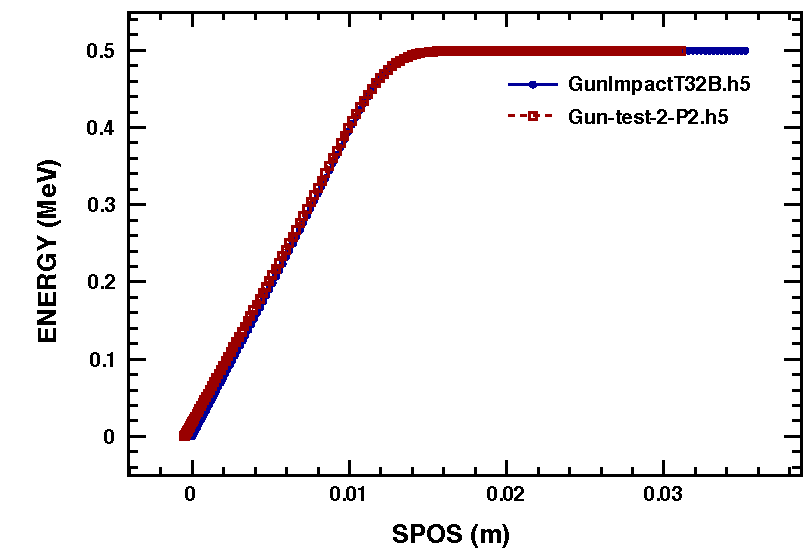
\includegraphics[width=0.45\textwidth]{figures/Gun/GunCompEn}
   \hspace{0.05\textwidth}
   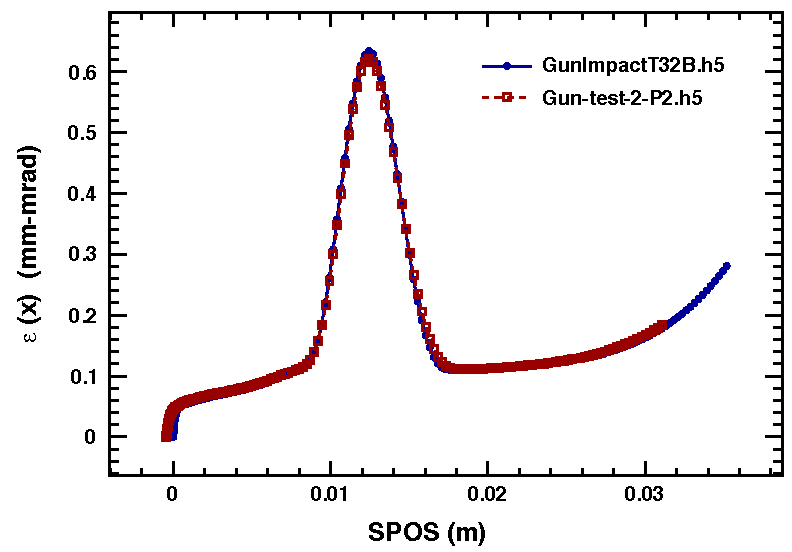
\includegraphics[width=0.45\textwidth]{figures/Gun/GunCompEx}
   \caption{Comparison of energy and emittance in $x$ between \impactt and \opalt}
   \label{fig:guncomp1}
\end{figure}
%===========================================================

\section{Field Maps from the FEMAXX 3D Eigenmode Solver}
\ifthenelse{\boolean{ShowDebug}}{
\TODO{AA will rewrite}

}{}
Electromagnetic field maps for beam dynamics calculations originate from a number of different
electromagnetic solvers, e.g. Superfish and similar codes.

Here, we describe the current status of work in progress which will, eventually,
allow the usage of field maps that have been computed with the FEMAXX $3$-dimensional
electromagnetic eigenmodal solver \cite{bib:arbenzetal2001,bib:arbenzetal2006}.

The FEMAXX code computes electromagnetic eigenmodes of resonant cavities of
arbitrary $3$-dimensional shape and boundary conditions.

Unlike Superfish and similar $2$-dimensional codes, FEMAXX is not restricted in the
kind of geometry it can model. It is therefore possible to consider arbitrary
shapes and their inclusion in beam dynamics and particle tracking calculations.

Given a mesh of a $3$-dimensional geometry FEMAXX computes eigenomdal field
decompositions.

The user then specifies sampling locations for the electromagnetic eigenfields.

At present, sampling locations are specified in terms of a cylinder shape,
i.e. the user indicates the cylinder axis, the radial cylinder vector and
the number of sampling locations in axial, radial and azimuthal directions.

Once the eigenmodal solution has been computed the fields are sampled at
these locations and stored in the T7 file format, for subsequent use in \opal.

Considerable effort has been spent for the validation and benchmarking of
beam dynamics calculations based on T7 field maps computed with FEMAXX.

A pillbox cavity, i.e. a cylinder shape with a radius $r = \SI{4.7}{\centi\meter}$ and
height $h = \SI{3}{\centi\meter}$, has been chosen for benchmarking purposes,
due to the availability of an analytical solution.

The analytical resonance frequency of the dominant mode is \SI{2.441}{\giga\hertz}.


%======================FIGURE===============================
\begin{figure}[!htb]
\centering
\includegraphics[width=0.6\textwidth]{./figures/adaptivePillboxMesh.pdf}
\caption[Tetrahedral mesh of a pillbox shaped cavity]{We show the discretization of a pillbox shaped cavity geometry into a tetrahedral mesh. The mesh has been adaptively refined so that the region around the cylinder axis is decomposed into smaller tetrahedra than those which are further away from the axis.}
\label{fig:pillbox_adaptively_refined_mesh}
\end{figure}
%===========================================================

We have compared two cases with \opal: (1) The analytical solution has been
sampled within a cylinder volume, stored into a T7 file and used in an \opal
run; (2) the same pillbox shaped geometry has been discretization into tetrahedra
and the eigenmodal fields were calculated with FEMAXX.
%%
These two cases were then compared, resulting in the following conclusions:
%%
(1) Using a relatively coarse mesh with some $110'000$ tetrahedra, the difference
between the analytical and the numerical solution was usually smaller than
$1$ percent.
%%
(2) Using an adaptively refined mesh, the difference between analytical and
numerical solutions decreased below $1$ per mill. The mesh is shown
in \figref{pillbox_adaptively_refined_mesh}.
%%
(3) It is therefore imperative to use a tetrahedral mesh which has been
refined around the beam axis. It is definitely more efficient to use local
refinement, based on physical argument, than simply refine the complete
mesh in a uniform manner.
%%


We are now working towards benchmarking more complicated shapes in order to
assess requirements w.r.t to meshes and modeling geometry so that we
achieve the same or better accuracy as has been obtained from field
maps that were computed with Superfish like solvers based on azimuthal symmetry.


\section{Output}
The phase space is stored in the H5hut file-format \cite{bib:howison2010} and can be analyzed
using e.g. H5root \cite{bib:schietinger}. The frequency
of the data output (phase space and some statistical quantities) can be controlled using the \keyword[sec:option]{OPTION} statement \seesec{option},
 with the flag \keyword{PSDUMPFREQ}. The file is named like in input file but with the extension {\tt .h5}.

A SDDS compatible ASCII file with statistical beam parameters is written to a file with extension {\tt .stat}. The frequency with which this data is written can be controlled with the \keyword[sec:option]{OPTION} statement \seesec{option} with the flag \keyword{STATDUMPFREQ}.
%======================FIGURE===============================
\begin{figure}[!htb]
\centering
 \includegraphics[width=0.32\textwidth]{figures/H5rootPicture1}
 \includegraphics[width=0.32\textwidth]{figures/H5rootPicture2}
 \includegraphics[width=0.31\textwidth]{figures/H5rootPicture3}
\caption[]{H5root enables a variety of data analysis and post processing task on \opal data}
%  \caption{Example of a longitudinal phase space shown with H5root}
 \label{fig:h5root1}
\end{figure}
%===========================================================

\section{Change History}
See \appref{changelog} for a detailed list of changes in \opal.
\section{Known Issues and Limitations}
\subsection{\opalcycl}
\begin{itemize}
    \item Restart with the option \keyword{PSDUMPLOCALFRAME} does not work yet,
    \item In complicated geometries such as spiral inflectors, proper particle deletion at the boundary sometimes fails.
\end{itemize}
\section{Acknowledgments}
The contributions of various individuals and groups are acknowledged in the relevant chapters, however a few individuals have or had considerable influence on the
development of \opal, namely Chris Iselin, John Jowett, Julian Cummings, Ji Qiang, Robert Ryne and Stefan Adam. For the \partroot~ visualization tool credits go to Thomas Schietinger.
The effort to couple FEMAXX to \opal was led by Benedikt Oswald.

The following
individuals are acknowledged for past contributions: Tulin Kaman, Yuanjie Bi, Colwyn Gulliford, Hao Zha and Christopher Mayes.

%- - - - - - - - - - - - - - - SECTION- - - - - - - - - - - - - - - - - - -
\section{Citation}
Please cite \opal in the following way:
\begin{example}
@techreport{opal:1,
title = {The OPAL (Object Oriented Parallel Accelerator Library) Framework},
author = {Andreas Adelmann and Achim Gsell and Valeria Rizzoglio (PSI) and Christof
Metzger-Kraus (HZB) and Yves Ineichen (IBM) and Xiaoying Pang and Steve Russell (LANL)
and Chuan Wang and Jianjun Yang (CIAE) and Suzanne Sheehy and Chris Rogers (RAL) and
Daniel Winklehner (MIT)},
institution = {Paul Scherrer Institut},
number = {PSI-PR-08-02},
year = {(2008-2016)}
}
\end{example}



%----------- Footer control ------------------
\ifthenelse{\boolean{FullOPALManual}}
{
  %do nothing
}
% else (for individual document creation)
{
\appendix
\printbibliography
\end{document}
}
%---------------------------------------------          % ch 1
\chapter{Conventions}

\label{chp:definitions}
\index{conventions|(}
\index{global!reference}
\index{reference!global}
The accelerator and/or beam line to be studied with \opalmap is described as
a sequence of beam elements placed sequentially along a reference or
design orbit.
The global reference orbit, also known as the \figref{design orbit}{global} 
is the path of a charged particle having the central design momentum 
of the accelerator through idealised magnets with no fringe fields.

In case of \opalt and \opalcycl with time as the independent variable no such 
explicit design orbit exists. The rest of this chapter is only relevant to 
\opalmap except Section \ref{sec:units} on the physical units. 


\section{Design or Reference Orbit}
\index{design!orbit}
\index{orbit!design}
\index{reference!orbit}
\index{orbit!reference}
The reference orbit consists of a series of
straight line segments and circular arcs.
It is defined under the assumption that all elements are
perfectly aligned along the design orbit.
The accompanying tripod of the reference orbit spans
a local curvilinear right handed coordinate system $(x,y,s)$.
The local $s$-axis is the tangent to the reference orbit.
The other two axes are perpendicular to the reference orbit and
are labelled~$x$ (in the bend plane)
and~$y$ (perpendicular to the bend plane).

\section{Closed Orbit}
\index{closed!orbit}
\index{orbit!closed}
\index{misalignment}
\index{field!error}
\index{error!field}
\index{error!misalignment}
\index{fringe field}
\index{field!fringe}
Due to various errors like misalignment errors, field errors,
fringe fields etc.,
the closed orbit does not coincide with the design orbit.
It also changes with the momentum error.
The closed orbit is described with respect to the reference orbit, 
using the \figref{local reference system}{local}.
It is evaluated including any nonlinear effects.

\begin{figure}[ht]
  \begin{center}
    \setlength{\unitlength}{1pt}
    \begin{picture}(400,250)
                                % axes
      \thicklines
      \put(180,100){\vector(0,1){90}}
      \put(180,0){\line(0,1){33.3}}
      \put(187,185){\makebox(0,0){$y$}}
      \put(280,0){\vector(-1,1){160}}
      \put(120,150){\makebox(0,0){$x$}}
      \thinlines
      \put(180,100){\circle*{4}}
                                % coordinates
      \put(150,130){\line(0,1){60}}
      \put(155,125){\line(0,1){60}}
      \put(160,120){\line(0,1){60}}
      \put(165,115){\line(0,1){60}}
      \put(170,110){\line(0,1){60}}
      \put(175,105){\line(0,1){60}}
      \put(180,160){\line(-1,1){30}}
      \put(180,150){\line(-1,1){30}}
      \put(180,140){\line(-1,1){30}}
      \put(180,130){\line(-1,1){30}}
      \put(180,120){\line(-1,1){30}}
      \put(180,110){\line(-1,1){30}}
                                % radius of curvature and centre
      \put(280,0){\vector(-3,1){172}}
      \put(160,30){\makebox(0,0){$\rho$}}
      \put(280,0){\vector(0,1){142}}
      \put(290,60){\makebox(0,0){$\rho$}}
      \put(280,0){\circle*{4}}
      \put(295,15){\vector(-1,-1){12}}
      \put(295,15){\makebox(0,0)[bl]{\shortstack{centre of \\curvature}}}
      \path(270,3.3)(280,9)
      \path(260,6.7)(280,18)
      \path(250,10)(280,27)
      \path(240,13.3)(280,36)
      \path(230,16.7)(280,45)
      \path(220,20)(280,54)
      \path(210,23.3)(280,63)
      \path(200,26.7)(280,72)
      \path(190,30)(280,81)
      \path(180,33.3)(280,90)
      \path(170,36.7)(280,99)
      \path(160,40)(280,108)
      \path(150,43.3)(280,117)
      \path(140,46.7)(280,126)
      \path(130,50)(280,135)
      \path(120,53.3)(278,142)
      \path(110,56.7)(218,117.9)
                                % actual orbit
      \thicklines
      \bezier{150}(0,100)(75,165)(150,190)
      \bezier{150}(150,190)(240,220)(320,220)
      \put(320,220){\vector(1,0){4}}
      \put(80,180){\vector(1,-1){12}}
      \put(80,180){\makebox(0,0)[br]{\shortstack{actual \\orbit}}}
                                % reference orbit
      \bezier{150}(40,0)(100,60)(180,100)
      \bezier{150}(180,100)(260,140)(340,160)
      \put(340,160){\vector(4,1){4}}
      \put(330,165){\makebox{$s$}}
      \put(320,135){\vector(-1,1){12}}
      \put(320,135){\makebox(0,0)[tl]{\shortstack{reference \\orbit}}}
    \end{picture}
    \caption{Local Reference System}
    \label{fig:local}
  \end{center}
\end{figure}

\index{betatron motion}
\index{synchrotron motion}
\opalmap computes the betatron and synchrotron oscillations
with respect to the closed orbit.
Results are given in the local $(x, y, s)$-system
defined by the reference orbit.

\section{Global Reference System}
\index{global!reference}
\index{reference!global}

The \figref{global reference orbit}{global} 
of the accelerator is uniquely defined by the sequence of physical elements.
The local reference system $(x, y, s)$
may thus be related to a global Cartesian coordinate system $(X, Y, Z)$.
The positions between beam elements are numbered $0, \ldots , i, \ldots n$.
The local reference system $(x_i, y_i, s_i)$ at position $i$,
i.e.\ the displacement and direction of the reference orbit
with respect to the system $(X, Y, Z)$ are defined by three displacements 
$(X_i, Y_i, Z_i)$ and three angles $(\Theta_i, \Phi_i, \Psi_i)$.

\begin{figure}[ht]%                                         1.2
  \begin{center}
    \setlength{\unitlength}{1pt}
    \begin{picture}(400,270)
                                % global axes
      \thicklines
      \put(20,150){\line(2,-1){40}}
      \dashline{3}(60,130)(100,110)
      \put(100,110){\line(2,-1){60}}
      \put(193,63){\vector(2,-1){90}}
      \put(300,20){\makebox(0,0){$Z$}}
      \put(20,100){\line(3,1){30}}
      \dashline{3}(50,110)(248,176)
      \put(248,176){\vector(3,1){132}}
      \put(373,210){\makebox(0,0){$X$}}
      \put(80,0){\vector(0,1){270}}
      \put(70,265){\makebox(0,0){$Y$}}
                                %local axes
      \put(133.3,0){\vector(1,3){90}}
      \put(215,270){\makebox(0,0){$x$}}
      \put(300,150){\vector(-2,1){160}}
      \put(140,220){\makebox(0,0){$y$}}
      \put(0,100){\vector(2,1){270}}
      \put(260,240){\makebox(0,0){$s$}}
                                % projection of s onto ZX
      \thinlines
      \put(100,110){\circle*{4}}
      \put(200,200){\circle*{4}}
      \path(0,110)(170,110)
      \dashline{3}(170,110)(240,110)
      \path(240,110)(290,110)
      \put(280,90){\makebox(0,0)[t]{\shortstack{projection of $s$ \\
            onto $(Z,X)$-plane}}}
      \put(280,95){\vector(0,1){13}}
      \put(20,110){\circle*{4}}
      \put(50,110){\circle*{4}}
                                % hashing of xy plane
      \path(210,195)(160,45)
      \path(220,190)(169.7,39.7)
      \path(230,185)(187.5,57.5)
      \path(240,180)(205,75)
      \path(250,175)(222.5,92.5)
      \path(260,170)(240,110)
      \path(270,165)(257.5,127.5)
      \path(280,160)(275,145)

      \path(196.7,190)(278.9,148.9)
      \path(193.3,180)(271.1,141.1)
      \path(190,170)(263.3,133.3)
      \path(186.7,160)(255.5,125.5)
      \path(183.3,150)(247.7,117.7)
      \path(180,140)(239.9,109.9)
      \path(176.7,130)(232.1,101.1)
      \path(173.3,120)(224.3,94.3)
      \path(170,110)(216.5,86.5)
      \path(166.7,100)(208.7,78.7)
      \path(163.3,90)(200.9,70.9)
      \path(160,80)(193.1,63.1)
      \path(156.7,70)(185.3,55.3)
      \path(153.3,60)(177.5,47.5)
      \path(150,50)(169.7,39.7)
                                % hashing of projection plane
      \put(70,110){\line(0,1){25}}
      \put(80,110){\line(0,1){30}}
      \put(90,110){\line(0,1){35}}
      \put(100,110){\line(0,1){40}}
      \put(110,110){\line(0,1){45}}
      \put(120,110){\line(0,1){50}}
      \put(130,110){\line(0,1){55}}
      \put(140,110){\line(0,1){60}}
      \put(150,110){\line(0,1){65}}
      \put(160,110){\line(0,1){70}}
      \put(170,110){\line(0,1){75}}
      \put(180,140){\line(0,1){50}}
      \put(190,170){\line(0,1){25}}
                                % intersection of xy and ZX
      \put(130,0){\line(1,1){230}}
      \put(135,5){\circle*{4}}
      \put(193.3,63.3){\circle*{4}}
      \put(240,110){\circle*{4}}
      \put(286.7,156.7){\circle*{4}}
      \put(335,205){\circle*{4}}
      \thicklines
      \put(200,25){\vector(-1,1){20}}
      \put(200,20){\makebox(0,0)[t]{\shortstack{intersection of \\
            $(x,y)$ and $(Z,X)$ planes}}}
                                % reference orbit
      \bezier{80}(140,150)(170,185)(200,200)
      \bezier{80}(200,200)(230,215)(260,220)
      \put(260,220){\makebox(0,0)[l]{\shortstack{reference \\orbit}}}
                                % roll angle
      \bezier{30}(160,30)(160,40)(150,50)
      \put(152,48){\vector(-1,1){2}}
      \put(150,30){\makebox(0,0){$\psi$}}
      \put(140,30){\makebox(0,0)[br]{roll angle}}
                                % pitch angle
      \bezier{20}(60,110)(60,120)(55,125)
      \put(57,123){\vector(-1,2){2}}
      \put(50,118){\makebox(0,0){$\phi$}}
      \put(40,125){\makebox(0,0)[br]{pitch angle}}
                                % azimuth
      \bezier{20}(130,95)(140,100)(140,110)
      \put(140,105){\vector(0,1){5}}
      \put(130,105){\makebox(0,0){$\theta$}}
      \put(115,95){\makebox(0,0)[t]{azimuth}}
    \end{picture}
    \caption{Global Reference System}
    \label{fig:global}
  \end{center}
\end{figure}

\index{displacement}
The above quantities are defined more precisely as follows:
\begin{description}
\item[X]
  \index{horizontal displacement}
  Displacement of the local origin in $X$-direction.
\item[Y]
  \index{vertical displacement}
  Displacement of the local origin in $Y$-direction.
\item[Z]
  \index{longitudinal displacement}
  Displacement of the local origin in $Z$-direction.
  \index{angle}
\item[THETA]
  \index{azimuth angle}
  Angle of rotation (azimuth) about the global $Y$-axis,
  between the global $Z$-axis and the projection
  of the reference orbit onto the $(Z, X)$-plane.
  A positive angle \texttt{THETA} forms a right-hand screw with the $Y$-axis.
\item[PHI]
  \index{pitch angle}
  Pitch angle, i.e. the angle between the reference orbit and its projection
  onto the $(Z, X)$-plane.
  A positive angle \texttt{PHI} correspond to $Y$ increasing with $s$.
  If only horizontal bends are present,
  the reference orbit remains in the ($Z$, $X$)-plane.
  In this case \texttt{PHI} is always zero.
\item[PSI]
  \index{roll angle}
  Roll angle about the local $s$-axis,
  i.e. the angle between the intersection $(x, y)$- and
  $(Z, X)$-planes and the local $x$-axis.
  A positive angle \texttt{PSI} forms a right-hand screw with the $s$-axis.
\end{description}
The angles \texttt{(THETA, PHI, PSI)} are \textbf{not} the Euler angles.
The reference orbit starts at the origin and points by default
in the direction of the positive $Z$-axis.
The initial local axes $(x, y, s)$ 
coincide with the global axes $(X, Y, Z)$ in this order.
The six quantities $(X_0, Y_0, Z_0, \Theta_0, \Phi_0, \Psi_0)$
thus all have zero initial values by default.
The program user may however specify different initial conditions.

Internally the displacement is described by a vector $V$
and the orientation by a unitary matrix $W$.
The column vectors of $W$ are the unit vectors spanning 
the local coordinate axes in the order $(x, y, s)$.
$V$ and $W$ have the values:
\[
V=\left(\begin{array}{c}
    X \\
    Y \\
    Z
  \end{array}\right),
\qquad
W=\Theta\Phi\Psi
\]
where
\[
\Theta=\left(\begin{array}{ccc}
    \cos\theta &  0 &  \sin\theta \\
    0         &  1 &   0 \\
    -\sin\theta &  0 &  \cos\theta
  \end{array}\right),
\quad
\Phi=\left(\begin{array}{ccc}
    1 &  0        &  0 \\
    0 &  \cos\phi &  \sin\phi \\
    0 & -\sin\phi &  \cos\phi
  \end{array}\right),
\quad
\]
\[
\Psi=\left(\begin{array}{ccc}
    \cos\psi & -\sin\psi &  0 \\
    \sin\psi &  \cos\psi &  0 \\
    0        &  0        &  1
  \end{array}\right).
\]

The reference orbit should be closed and it should not be twisted.
This means that the displacement of the local reference system
must be periodic with the revolution frequency of the accelerator,
while the position angles must be periodic $\pmod{2\pi}$
with the revolution frequency.
If \texttt{PSI} is not periodic $\pmod{2\pi}$, 
coupling effects are introduced.
When advancing through a beam element,
\opalmap computes $V_i$ and $W_i$
by the recurrence relations
\[
V_i = W_{i-1}R_i + V_{i-1}, \qquad
W_i = w_{i-1}S_i.
\]

The vector $R_i$ is the displacement and the matrix
$S_i$ is the rotation of the local reference system 
at the exit of the element $i$ with respect to the entrance 
of the same element.
The values of $R_i$ and $S_i$
are listed below for each physical element type.

\section{Local Reference Systems}
\index{local!reference}
\index{reference!local}
\subsection{Reference System for Straight Beam Elements}
\label{sec:straight}
In straight elements the \figref{local reference system}{straight} 
is simply translated by the length of the element along the local $s$-axis.
This is true for
\begin{itemize}
\item \secref{Drift spaces}{drift}
\item \secref{Quadrupoles}{quadrupole}
\item \secref{Sextupoles}{sextupole}
\item \secref{Octupoles}{octupole}
\item \secref{Multipoles}{octupole}
\item \secref{Solenoids}{solenoid}
\item \secref{RF cavities}{cavity}
\item \secref{Electrostatic separators}{separator}
\item \secref{Closed orbit correctors}{corrector}
\item \secref{Beam position monitors}{monitors}
\end{itemize}
The corresponding $R$, $S$ are
\[
R=\left(\begin{array}{c}
    0 \\
    0 \\
    L
  \end{array}\right),
\qquad
S=\left(\begin{array}{ccc}
    1 & 0 & 0 \\
    0 & 1 & 0 \\
    0 & 0 & 1 \\
  \end{array}\right).
\]
A rotation of the element about the $S$-axis has no effect
on $R$ and $S$, since the rotations of the reference system 
before and after the element cancel.

\begin{figure}[ht]
  \begin{center}
    \setlength{\unitlength}{1pt}
    \begin{picture}(400,100)
      \thinlines
                                % axes
      \put(150,50){\circle{8}}\put(150,50){\circle*{2}}
      \put(140,40){\makebox(0,0){$y_1$}}
      \put(250,50){\circle{8}}\put(250,50){\circle*{2}}
      \put(260,40){\makebox(0,0){$y_2$}}
      \put(100,50){\line(1,0){46}}
      \put(154,50){\line(1,0){92}}
      \put(254,50){\vector(1,0){46}}
      \put(290,40){\makebox(0,0){$s$}}
      \put(150,0){\line(0,1){46}}
      \put(150,54){\vector(0,1){46}}
      \put(140,90){\makebox(0,0){$x_1$}}
      \put(250,0){\line(0,1){46}}
      \put(250,54){\vector(0,1){46}}
      \put(260,90){\makebox(0,0){$x_2$}}
                                % magnet outline
      \thicklines
      \put(150,54){\line(0,1){26}}
      \put(150,46){\line(0,-1){26}}
      \put(250,54){\line(0,1){26}}
      \put(250,46){\line(0,-1){26}}
      \put(150,20){\line(1,0){100}}
      \put(150,80){\line(1,0){100}}
      \put(200,2){\vector(1,0){50}}
      \put(200,2){\vector(-1,0){50}}
      \put(200,10){\makebox(0,0){L}}
    \end{picture}
    \caption{Reference System for Straight Beam Elements}
    \label{fig:straight}
  \end{center}
\end{figure}

\subsection{Reference System for Bending Magnets}
\label{rbend}
Both \figref{rectangular}{rbend} and \figref{sector}{sbend}
bending magnets have a curved reference orbit.
For both types of magnets
\[
R=\left(\begin{array}{c}
    \rho(\cos\alpha-1) \\
    0 \\
    \rho\sin\alpha
  \end{array}\right),
\qquad
S=\left(\begin{array}{ccc}
    \cos\alpha & 0 & -\sin\alpha \\
    0          & 1 &  0 \\
    \sin\alpha & 0 &  \cos\alpha
  \end{array}\right),
\]
where $\alpha$ is the bend angle.
A positive bend angle represents a bend to the right,
i.e. towards negative $x$ values.
For sector bending magnets,
the bend radius is given by $\rho$,
and for rectangular bending magnets it has the value
\[
\rho = L / 2 \sin(\alpha/2).
\]
If the magnet is rotated about the $s$-axis by an angle psi,
$R$ and $S$ are transformed by
\[
R^{*} = T R, \qquad S^{*} = T S T^{-1}.
\]
where $T$ is the orthogonal rotation matrix
\[
T=
\begin{pmatrix}
    \cos\psi & -\sin\psi &  0 \\
    \sin\psi &  \cos\psi &  0 \\
    0        &  0        &  1 
\end{pmatrix}.
\]
The special value $\psi = \pi/2$ represents a bend down.

\begin{figure}[ht]
  \begin{center}
    \setlength{\unitlength}{1pt}
    \begin{picture}(400,215)
                                % axes
      \thinlines
      \put(150,150){\circle{8}}\put(150,150){\circle*{2}}
      \put(160,140){\makebox(0,0){$y_1$}}
      \put(250,150){\circle{8}}\put(250,150){\circle*{2}}
      \put(240,140){\makebox(0,0){$y_2$}}
      \put(74,124.7){\vector(3,1){72}}
      \put(84,135){\makebox(0,0){$s_1$}}
      \put(254,148.7){\vector(3,-1){72}}
      \put(316,135){\makebox(0,0){$s_2$}}
      \put(200,0){\vector(-1,3){48.7}}
      \put(165,75){\makebox(0,0){$\rho$}}
      \put(148.7,154){\vector(-1,3){18}}
      \put(118,206){\makebox(0,0){$x_1$}}
      \put(200,0){\vector(1,3){48.7}}
      \put(235,75){\makebox(0,0){$\rho$}}
      \put(251.3,154){\vector(1,3){18}}
      \put(282,206){\makebox(0,0){$x_2$}}
      \bezier{20}(190.5,28.5)(200,31.7)(209.5,28.5)
      \put(200,20){\makebox(0,0){$\alpha$}}
      \put(154,150){\line(1,0){92}}
      \put(200,150){\circle*{4}}
      \put(200,150){\vector(0,1){60}}
      \put(210,200){\makebox(0,0){$x$}}
      \put(150,154){\line(0,1){44}}
      \put(150,146){\line(0,-1){46}}
      \put(151,154){\line(1,4){11}}
      \put(250,154){\line(0,1){44}}
      \put(250,146){\line(0,-1){46}}
      \put(249,154){\line(-1,4){11}}
                                % magnet outline
      \thicklines
      \put(200,102){\vector(-1,0){50}}
      \put(200,102){\vector(1,0){50}}
      \put(200,110){\makebox(0,0){L}}
      \put(151,154){\line(1,4){6}}
      \put(149,146){\line(-1,-4){6}}
      \put(249,154){\line(-1,4){6}}
      \put(251,146){\line(1,-4){6}}
      \put(157,178){\line(1,0){86}}
      \put(143,122){\line(1,0){114}}
      \bezier{10}(150,195)(155.5,195)(160.9,193.7)
      \put(155.5,195){\vector(3,-1){5.4}}
      \put(150,205){\makebox(0,0)[l]{$e_1$}}
      \bezier{10}(250,195)(244.5,195)(239.1,193.7)
      \put(244.5,195){\vector(-3,-1){5.4}}
      \put(250,205){\makebox(0,0)[r]{$e_2$}}
    \end{picture}
    \caption[Reference System for a Rectangular Bending Magnet]%
    {Reference System for a Rectangular Bending Magnet;
      the signs of pole-face rotations are positive as shown.}
    \label{fig:rbend}
  \end{center}
\end{figure}

\begin{figure}[ht]
  \begin{center}
    \setlength{\unitlength}{1pt}
    \begin{picture}(400,215)
                                % axes
      \thinlines
      \put(150,150){\circle{8}}\put(150,150){\circle*{2}}
      \put(160,140){\makebox(0,0){$y_1$}}
      \put(250,150){\circle{8}}\put(250,150){\circle*{2}}
      \put(240,140){\makebox(0,0){$y_2$}}
      \put(74,124.7){\vector(3,1){72}}
      \put(84,135){\makebox(0,0){$s_1$}}
      \put(254,148.7){\vector(3,-1){72}}
      \put(316,135){\makebox(0,0){$s_2$}}
      \put(200,0){\vector(-1,3){48.7}}
      \put(165,75){\makebox(0,0){$\rho$}}
      \put(148.7,154){\vector(-1,3){18}}
      \put(118,206){\makebox(0,0){$x_1$}}
      \put(200,0){\vector(1,3){48.7}}
      \put(235,75){\makebox(0,0){$\rho$}}
      \put(251.3,154){\vector(1,3){18}}
      \put(282,206){\makebox(0,0){$x_2$}}
      \bezier{20}(190.5,28.5)(200,31.7)(209.5,28.5)
      \put(200,20){\makebox(0,0){$\alpha$}}
      \put(200,158.8){\circle*{4}}
      \put(200,158.8){\vector(0,1){50}}
      \put(210,200){\makebox(0,0){$r$}}
      \put(151,154){\line(1,4){10}}
      \put(249,154){\line(-1,4){10}}
                                % magnet outline
      \thicklines
      \bezier{100}(154,151.3)(200,166.7)(246,151.3)
      \put(162,154){\vector(-3,-1){8}}
      \put(238,154){\vector(3,-1){8}}
      \put(210,168){\makebox(0,0){L}}
      \put(151,154){\line(1,4){6}}
      \put(149,146){\line(-1,-4){6}}
      \put(249,154){\line(-1,4){6}}
      \put(251,146){\line(1,-4){6}}
      \bezier{90}(157,178)(200,188.4)(243,178)
      \bezier{110}(143,122)(200,148.6)(257,122)
      \bezier{20}(137.4,187.9)(149.1,191.5)(159.7,188.8)
      \put(153.7,190.8){\vector(3,-1){6}}
      \put(150,180){\makebox(0,0){$e_1$}}
      \bezier{20}(262.6,187.9)(250.9,191.5)(240.3,188.8)
      \put(246.3,190.8){\vector(-3,-1){6}}
      \put(250,180){\makebox(0,0){$e_2$}}
    \end{picture}
    \caption[Reference System for a Sector Bending Magnet]%
    {Reference System for a Sector Bending Magnet;
      the signs of pole-face rotations are positive as shown.}
    \label{fig:sbend}
  \end{center}
\end{figure}

\subsection{Rotation of the Reference System}
\label{sec:refrot}
For a 
\figref{rotation of the reference system by an angle $\psi$ about the
  beam ($s$) axis}{srot}: 
\[
S=\left(\begin{array}{ccc}
    \cos\psi & -\sin\psi &  0 \\
    \sin\psi &  \cos\psi &  0 \\
    0        &  0        &  1 \\
  \end{array}\right),
\]
while for a 
\figref{rotation of the reference system by an angle $\theta$ about
  the vertical ($y$) axis}{yrot}:
\[
S=\left(\begin{array}{ccc}
    \cos\theta &  0 & -\sin\theta \\
    0          &  1 &  0 \\
    \sin\theta &  0 &  \cos\theta
  \end{array}\right).
\]
In both cases the displacement $R$ is zero.

\begin{figure}[ht]%
  \begin{center}
    \setlength{\unitlength}{1pt}
    \begin{picture}(400,200)
      \thinlines
      \put(200,100){\circle{8}}\put(200,100){\circle*{2}}
      \put(190,90){\makebox(0,0){$s$}}
      \put(100,100){\line(1,0){96}}
      \put(204,100){\vector(1,0){96}}
      \put(290,90){\makebox(0,0){$x_1$}}
      \put(200,0){\line(0,1){96}}
      \put(200,104){\vector(0,1){96}}
      \put(190,210){\makebox(0,0){$y_1$}}
      \put(103,75.75){\line(4,1){93}}
      \put(204,101){\vector(4,1){93}}
      \put(287,134){\makebox(0,0){$x_2$}}
      \put(224.25,3){\line(-1,4){23.25}}
      \put(199,104){\vector(-1,4){23.25}}
      \put(166,187){\makebox(0,0){$y_2$}}
      \bezier{20}(260,100)(260,107.5)(258,114.5)
      \put(260,106.5){\vector(-1,4){2}}
      \put(250,106.25){\makebox(0,0){$\psi$}}
      \put(220,150){\circle{8}}\put(220,150){\circle*{2}}
      \put(220,140){\makebox(0,0){beam}}
    \end{picture}
    \caption{Reference System for a Rotation Around the s-Axis}
    \label{fig:srot}
  \end{center}
\end{figure}

\begin{figure}[ht]%
  \begin{center}
    \setlength{\unitlength}{1pt}
    \begin{picture}(400,200)
      \thinlines
      \put(200,100){\circle{8}}\put(200,100){\circle*{2}}
      \put(190,90){\makebox(0,0){$y$}}
      \put(100,100){\line(1,0){96}}
      \put(204,100){\vector(1,0){96}}
      \put(290,110){\makebox(0,0){$s_1$}}
      \put(200,0){\line(0,1){96}}
      \put(200,104){\vector(0,1){96}}
      \put(190,190){\makebox(0,0){$x_1$}}
      \put(103,124.25){\line(4,-1){93}}
      \put(204,99){\vector(4,-1){93}}
      \put(287,66){\makebox(0,0){$s_2$}}
      \put(175.75,3){\line(1,4){23.25}}
      \put(201,104){\vector(1,4){23.25}}
      \put(234,187){\makebox(0,0){$x_2$}}
      \bezier{20}(260,100)(260,92.5)(258,85.5)
      \put(260,93.5){\vector(-1,-4){2}}
      \put(250,93.75){\makebox(0,0){$\theta$}}
      \thicklines
      \put(100,130){\vector(1,0){200}}
      \put(290,140){\makebox(0,0){beam}}
    \end{picture}
    \caption{Reference System for a Rotation Around the y-Axis}
    \label{fig:yrot}
  \end{center}
\end{figure}

\subsection{Elements which do not Change the Local Reference}
The following elements do not affect the
reference orbit and are ignored for geometry calculations:
\begin{itemize}
\item Beam-beam interactions %\secref{Beam-beam interactions}{sec:beambeam}
\item \secref{Marker}{marker}
\end{itemize}

\section{Sign Conventions for Magnetic Fields}
\label{sec:sign}
\index{sign conventions for fields}
\index{field!signs}
The \opalmap program uses the following Taylor expansion for the normal and
skewed field components respectively in the mid-plane $y$=0, 
described in \bibref{SLAC-75}{matrix}:
\[
B_x(x,0)=\sum_{k=0}^{\infty}\frac{B_{kn}x^k}{k!}, \qquad
B_x(x,0)=\sum_{k=0}^{\infty}\frac{B_{ks}x^k}{k!}.
\]
Note the factorial in the denominator.
The field coefficients have the following meaning:
\begin{description}
\item[$B_{0n}$] Normal dipole field component.
  The component is positive if the field points in the positive $y$
  direction. 
  A positive field bends a positively charged particle travelling in
  positive $s$-direction to the right.
\item[$B_{0s}$] Skew dipole field component.
  The component is positive if the field points in the negative $y$
  direction. 
  A positive field bends a positively charged particle travelling in
  positive $s$-direction down.
\item[$B_{1n}$] Normal quadrupole field component
  $B_{1n}=\partial B_y/\partial x$.
  The component is positive if $B_y$ is positive on the positive $x$-axis.
  A positive value corresponds to horizontal focussing of a positively
  charged particle.
\item[$B_{1s}$] Skew quadrupole field component
  $B_{1s}=\partial B_x/\partial x$.
  The component is positive if $B_x$ is negative on the positive $x$-axis.
\item[$B_{2n}$] Normal sextupole field component
  $B_{2n}=\partial^2 B_y/\partial x^2$.
  The component is positive if $B_y$ is positive on the $x$-axis.
\item[$B_{2s}$] Skew sextupole field component
  $B_{2s}=\partial^2 B_x/\partial x^2$.
  The component is negative if $B_x$ is positive on the $x$-axis.
\item[$B_{3n}$] Normal octupole field component
  $B_{3n}=\partial^3 B_y/\partial x^3$.
  The component is positive if $B_y$ is positive on the positive $x$-axis.
\item[$B_{3s}$] Skew octupole field component
  $B_{3s}=\partial^3 B_x/\partial x^3$.
  The component is negative if $B_x$ is positive on the $x$-axis.
\end{description}
All derivatives are taken on the $x$-axis.
Using this expansion and the curvature $h$ of the reference orbit,
the longitudinal component of the vector potential for a magnet with
mid-plane symmetry is to order~4:
\index{field!vector potential}
\index{vector potential}

\begin{align*} 
  A_s \quad = \quad 
  & B_{0n}\left(x-\frac{hx^2}{2(1+hx)}\right) \\
  &+B_{1n}\left(\frac{1}{2}(x^2-y^2)-\frac{h}{6}x^{3}
  +\frac{h^2}{24}(4x^{4}-y^{4})+\ldots\right) \\
  &+B_{2n}\left(\frac{1}{6}(x^{3}-3xy^2)-\frac{h}{24}(x^{4}-y^{4})
   +\ldots\right) \\
  &+B_{3n}\left(\frac{1}{24}(x^{4}-6x^2y^2+y^{4})+\ldots\right)
   + \ldots
\end{align*}
Taking $\mathrm{curl} A$ in curvilinear coordinates,
the field components can be computed as
\index{field!components}
\begin{align*} 
  B_x(x,y) \quad = \quad
  & B_{1n}\left(y+\frac{h^2}{6}y^{3}+\ldots\right) 
   +B_{2n}\left(xy-\frac{h^{3}}{6}y^{3}+\ldots\right) \\
  &+B_{3n}\left(\frac{1}{6}(3x^2y-y^{3})+\ldots\right) + \ldots \\
  B_y(x,y) \quad = \quad 
  & B_{0n}
   +B_{1n}\left(x-\frac{h}{2}y^2+\frac{h^2}{2}xy^2+\ldots\right) \\
  &+B_{2n}\left(\frac{1}{2}(x^2-y^2)-\frac{h}{2}xy^2+\ldots\right) \\
  &+B_{3n}\left(\frac{1}{6}(x^{3}-3xy^2)+\ldots\right) + \ldots
\end{align*}
One can easily verify that both $\mathrm{curl} B$ and $\mathrm{div} B$
are zero to the order of the $B_3$ term.
Introducing the magnetic rigidity $B \rho$,
the multipole coefficients are computed as
\[
K_{kn}=eB_{kn}/p_0=B_{kn}/B\rho,\qquad
K_{ks}=eB_{ks}/p_0=B_{ks}/B\rho.
\]
Note that the $K_k$ have the \textbf{same sign} as the corresponding
field components $B_k$.
The signs will be changed due to the sign of particle charges and
the direction of travel of the beam.

\section{Variables in \opalt}
\label{sec:variablesopalt}
\index{variablesopalt}
For each variable the physical units are listed in square brackets.

\subsection{Variables Describing Orbits}
\label{sec:opalt:canon}
\index{canonical variables}
\index{variables!canonical}
\opalt uses the following canonical variables
to describe the motion of particles:

\begin{description}
\item[X]
  Horizontal position $x$ of a particle relative to the axis of the element [m].

\item[PX]
  Horizontal canonical momentum:
  $\mathtt{PX} = \beta_x \gamma$.

\item[Y]
  Horizontal position $y$ of a particle relative to the axis of the element [m].

\item[PY]
  Horizontal canonical momentum:
  $\mathtt{PY} = \beta_y \gamma$.

\item[Z]
  Longitudinal position $z$ of a particle in floor co-ordinates [m].

\item[PZ]
 Longitudinal canonical momentum: 
 $\mathtt{PZ} = \beta_z \gamma$.

 \end{description}

The independent variable is:
\begin{description}
\item[t]
  Time [s].
\end{description}

\section{Variables in \opalcycl}
\label{sec:variablesopalcycl}
\index{variablesopalcycl}

\subsection{Variables Describing Orbits}
\label{sec:opalcycl:canon}
\index{canonical variables}
\index{variables!canonical}

\opalcycl uses the following canonical variables to describe the motion of particles:

\begin{description}
\item[X]
  Horizontal position $x$ of a particle in given global Cartesian coordinates [m].

\item[PX]
  Horizontal momentum:
  $\mathtt{PX}$ rad.

\item[Y]
  Horizontal position $x$ of a particle in global Cartesian coordinates [m].

\item[PY]
  Horizontal canonical momentum:
  $\mathtt{PY} $ rad.

\item[Z]
  Vertical position $z$ of a particle in global Cartesian coordinates [m].

\item[PZ]
  Vertical canonical momentum:
  $\mathtt{PZ}  $ rad.

\end{description}

The independent variable is: \textbf{t} [s].


\subsubsection{Unit Conversion}
Convert the unit of momentum from $\beta \gamma$ to
$mrad$.

\begin{equation}
\label{eq:betagamma1}
(\beta\gamma)_z=\frac{P}{m_0c}=\frac{Pc}{m_0c^2}.
\end{equation}
\begin{equation}
\label{eq:betagamma2} P_x[
mrad]=1000\frac{P_x[\beta\gamma]}{(\beta\gamma)_z}
\end{equation}

Convert the unit from eV to $\beta\gamma$.
\begin{equation}
\label{eq:eVtobetagamma}
\sqrt{(\frac{T}{m_0c^2}+1)^2-1}=\beta\gamma.
\end{equation}




\subsection{Local frame initial distribution}
\label{sec:opalcycl:localframe}
To ensure compatibility with \opalt and \opalmap 
the initial distribution of the bunch,
either read from file or generated by specifying rms beam quantities,
is specified in the local Cartesian coordinates.
During run time,the 6 phase space variables \((x, y, z, p_x, p_y, p_z)\) 
are transformed to the global Cartesian coordinates
using initial reference $r_0$,$\theta_0$ and $p_{r0}$, $p_{\theta 0}$.
These 4 parameters are defined at the \secref{\texttt{CYCLOTRON} command }{cyclotron}
before particle tracking starts. 

\begin{align*}  
X &= x\cos(\theta_0) - y\sin(\theta_0) + r_0\cos(\theta_0)  \\
Y &= x\sin(\theta_0) + y\cos(\theta_0) + r_0\sin(\theta_0)  \\
Z &= z 
\end{align*}
\begin{align*}  
PX &= (p_x+p_{r0})\cos(\theta_0) - (p_y+p_{\theta 0})\sin(\theta_0) \\
PY &= (p_x+p_{r0})\sin(\theta_0) + (p_y+p_{\theta 0})\cos(\theta_0) \\
PZ &= p_z 
\end{align*}    

\section{Variables in \opalmap}
\label{sec:variables}
\index{variables}
For each variable the physical units are listed in square brackets.

\subsection{Canonical Variables Describing Orbits}
\label{sec:canon}
\index{canonical variables}
\index{variables!canonical}
\opalmap uses the following canonical variables
to describe the motion of particles:

\begin{description}
\item[X]
  Horizontal position $x$ of the (closed) orbit,
  referred to the ideal orbit [m].

\item[PX]
  Horizontal canonical momentum of the (closed) orbit referred 
  to the ideal orbit, divided by the reference momentum:
  $\mathtt{PX} = p_x / p_0$.

\item[Y]
  Vertical position $y$ of the (closed) orbit,
  referred to the ideal orbit [m].

\item[PY]
  Vertical canonical momentum of the (closed) orbit referred 
  to the ideal orbit, divided by the reference momentum:
  $\mathtt{PY} = p_y / p_0$.

\item[T]
  The negative time difference, 
  multiplied by the instantaneous velocity of the particle [m]:
  $\mathtt{T} = - v \delta(t)$.
  A positive \texttt{T} means that the particle arrives ahead of the 
  \textbf{reference particle}.
  \texttt{T} describes the deviation of the particle from the orbit of 
  a fictitious reference particle having the constant 
  \textbf{reference momentum} $p_s$ and the 
  \textbf{reference velocity} $v_s$.
  $v_s$ defines the revolution frequency.
  The velocities have the values 
  \[
  v = c p / \sqrt{p^2 + m^2 c^2}, \qquad
  v_s = c p_s / \sqrt{p_s^2 + m^2 c^2},
  \]
  where $c$ is the velocity of light, $m$ is the particle rest mass, 
  and $p$ is the instantaneous momentum of the particle.

\item[PT]
  Momentum error, divided by the reference momentum:
  $\mathtt{PT} = \delta p / p_s$.
  This value is only non-zero when synchrotron motion is present.
  It describes the deviation of the particle from the orbit of a
  particle with the reference momentum $p_s$.
\end{description}

The independent variable is:
\begin{description}
\item[S]
  Arc length $s$ along the reference orbit [m].
\end{description}

The longitudinal variables is in the limit of fully relativistic particles
($\gamma \gg 1, v = c, p c = E$),
the variables \texttt{T, PT} used here agree with the longitudinal variables
used in \bibref{TRANSPORT}{transport}.
This means that \texttt{T} becomes the negative path length difference,
while \texttt{PT} is the fractional momentum error.
The reference momentum must be constant in order to keep the system 
canonical.

\subsection{Normalised Variables and other Derived Quantities}
\label{sec:normal}
\index{normalised variables}
\index{variables!normalised}
\begin{description}
\item[XN]
  The normalised horizontal displacement [$\mathrm{m}^{1/2}$]:
  $\mathtt{XN} = x_n = \Re(E_1^T S Z)$.

\item[PXN]
  The normalised horizontal transverse momentum [$\mathrm{m}^{1/2}$]:
  $\mathtt{PXN} = p_{xn} = \Im(E_1^T S Z$).

\item[WX]
  The horizontal Courant-Snyder invariant [m]:
  $\mathtt{WX} = \sqrt{x_n^2 + p_{xn}^2}$.

\item[PHIX]
  The horizontal phase:
  $\mathtt{PHIX} = - \arctan(p_{xn} / x_n) / 2 \pi$.

\item[YN]
  The normalised vertical displacement [$\mathrm{m}^{1/2}$]:
  $\mathtt{YN} = y_n = \Re(E_2^T S Z)$.

\item[PYN]
  The normalised vertical transverse momentum [$\mathrm{m}^{1/2}$]:
  $\mathtt{PYN} = p_{yn} = \Im(E_2^T S Z)$.

\item[WY]
  The vertical Courant-Snyder invariant [m]:
  $\mathtt{WY} = \sqrt{y_n^2 + p_{yn}^2}$.

\item[PHIY]
  The vertical phase:
  $\mathtt{PHIY} = - \arctan(p_{yn} / y_n) / 2 \pi$.

\item[TN]
  The normalised longitudinal displacement [$\mathrm{m}^{1/2}$]:
  $\mathtt{TN} = t_n = \Re(E_3^T S Z)$.

\item[PTN]
  The normalised longitudinal transverse momentum [$\mathrm{m}^{1/2}$]:
  $\mathtt{PTN} = p_{tn} = Im(E_3^T S Z)$.

\item[WT]
  The longitudinal invariant [m]:
  $\mathtt{WT} = \sqrt{t_n^2 + p_{tn}^2}$.

\item[PHIT]
  The longitudinal phase:
  $\mathtt{PHIT} = + \arctan(p_{tn} / t_n) / 2 \pi$.

\end{description}
in the above formulas $Z$ is the phase space vector
$Z = (x, p_x, y, p_y, t, p_t)^T$.
The matrix $S$ is the ``symplectic unit matrix''
\[
S = 
\begin{pmatrix} 
    0 & 1 & 0 & 0 & 0 & 0 \\
   -1 & 0 & 0 & 0 & 0 & 0 \\
    0 & 0 & 0 & 1 & 0 & 0 \\
    0 & 0 &-1 & 0 & 0 & 0 \\
    0 & 0 & 0 & 0 & 0 & 1 \\
    0 & 0 & 0 & 0 &-1 & 0
  \end{pmatrix},
\]
and the vectors $E_i$ are the three complex eigenvectors.
The superscript $T$ denotes the transpose of a vector or matrix.

\section{Physical Units}
\label{sec:units}
\index{units}
\index{physical units}
Throughout the computations \opal uses \tabref{international units}{units},
as defined by SI (Syst\`eme International).

\begin{table}[ht] \footnotesize
  \begin{center}
    \caption{Physical Units}
    \label{tab:units}
    \begin{tabular}{|l|l|} 
      \hline
      quantity                         & dimension \\
      \hline
      Length                           & m (metres) \\
      Angle                            & rad (radians) \\
      Quadrupole coefficient           & $\mathrm{m}^{-2}$ \\
      Multipole coefficient, 2n poles  & $\mathrm{m}^{-n}$ \\
      Electric voltage                 & MV (Megavolts) \\
      Electric field strength          & MV/m \\
      Frequency                        & MHz (Megahertz) \\
      Phase angles                     & $2\pi$ \\
      Particle energy                  & GeV \\
      Particle mass                    & GeV/$c^2$ \\
      Particle momentum                & GeV/c \\
      Beam current                     & A (Amperes) \\
      Particle charge                  & e (elementary charges) \\
      Impedances                       & M$\Omega$ (Megohms) \\
      Emittances                       & $\pi$ m mrad \\
      Emittances \opalt             & m rad \footnote{(normalized and un-normalized)}\\
      RF power                         & MW (Megawatts) \\
      Higher mode loss factor          & V/pc \\
      \hline
    \end{tabular}
  \end{center}
\end{table}

\index{conventions|)}
           % ch 2
\ifdefined \buildingFullOPALManual \else


%\ifx \@buildingFullOPALManual \@empty
%\else

%\documentclass[12pt,a4paper]{report}
\documentclass[a4paper]{book}

%% does not work in Latex2Html mode
%\usepackage{hyperref}

\usepackage[T1]{fontenc}
\usepackage{url}
\usepackage{html}
\usepackage{epic}
\usepackage{eepic}
\usepackage{makeidx}
\usepackage{array}
\usepackage{times}
\usepackage{amsmath}
\usepackage{amsxtra}
\usepackage{bm}
\usepackage[thin,thinp,thinc]{esdiff}
\usepackage{etoolbox}
\usepackage{graphicx}
\usepackage{dingbat}
\usepackage{color}
\usepackage{subfig}
\usepackage{boxedminipage}
\usepackage{alltt}
\usepackage{nicefrac}
\usepackage{calc}
%\usepackage{pdfdraftcopy}             % Draft
\usepackage{tikz}
\usetikzlibrary{
  er,3d,calc,fadings,trees,positioning,arrows,chains,decorations.pathreplacing,
  decorations.pathmorphing,shapes,shapes.symbols,shapes.arrows,matrix,through,decorations.text
}

\tikzset{
  >=stealth',
  punktchain/.style={rectangle,rounded corners, draw=black, very thick,text width=10em,
                     minimum height=3em, text centered, on chain},
  line/.style={draw, thick, <-},
  element/.style={tape,top color=white,bottom color=blue!50!black!60!,minimum width=8em,
                  draw=blue!40!black!90, very thick,text width=10em, minimum height=3.5em,
                  text centered, on chain},
  every join/.style={->, thick,shorten >=1pt},
  tuborg/.style={decorate},
  tubnode/.style={midway, right=2pt}
}

\tikzstyle{material}=[draw, fill=blue!20, text width=16.0em, text centered, minimum height=1.5em]
\tikzstyle{diagramstep} = [material, text width=20em, minimum width=10em, minimum height=3em, rounded corners]
\tikzstyle{line} = [draw, thick, color=black!50, -latex']

\usepackage{booktabs}
\usepackage{xspace}
\usepackage{xstring}

\usepackage{fancyvrb}
\usepackage{rotating}
\usepackage{float}

\usepackage{tabularx}
\usepackage{longtable}
\setcounter{LTchunksize}{3}

\usepackage[section]{placeins}
\usepackage{MnSymbol}
\usepackage{microtype}
\usepackage{setspace}
\usepackage{dcolumn}

\usepackage[vmargin={3.0cm,3.0cm},
            hmargin={2.0cm,3.0cm}]{geometry}

\usepackage{upgreek}
\usepackage[binary-units=true]{siunitx}
\sisetup{exponent-product = \cdot,math-ohm=\Upomega,text-ohm=\ensuremath{\Upomega}}
\DeclareSIUnit{\clight}{c}
\DeclareSIUnit\gauss{Ga}

\usepackage{engord}
\usepackage{wasysym}
\DeclareSIUnit[number-unit-product = \,]{\permill}{\permil}

\usepackage{hyperref}
\hypersetup{
    pdftitle          = The OPAL Framework,
    pdfauthor         = {Andreas Adelmann, Achim Gsell, Valeria Rizzoglio, Christof Metzger-Kraus,
                         Yves Ineichen, Xiaoying Pang, Steve Russell, Chuan Wang, Jianjun Yang,
                         Suzanne Sheehy, Chris Rogers, Daniel Winklehner},
    pdfsubject        = User's Reference Manual,
    pdffitwindow      = true,               % page fit to window when opened
    pdfnewwindow      = true,               % links in new window
    colorlinks        = true,               % false: boxed links; true: colored links
    linkcolor         = black!80!green,     % color of internal links
    citecolor         = black!20!red,       % color of links to bibliography
    urlcolor          = blue,               % color of external links
    breaklinks        = true,
    bookmarksnumbered = true,
    plainpages        = false
}

\usepackage{ifthen}

\newif \iflinuxwindows
\linuxwindowstrue   % set this to true when building the manual on Linux or Windows
\iflinuxwindows
\usepackage{epstopdf}
\fi

\usepackage[backend=biber,
            style=phys,
            biblabel=brackets,
            maxnames=3,
            doi=true,
            isbn=true,
            url=true]{biblatex}
%---- macros ----

\renewcommand{\topfraction}{1.0}
\renewcommand{\bottomfraction}{1.0}
\renewcommand{\textfraction}{0.0}
\renewcommand{\arraystretch}{2.0}
\newenvironment{tex2html_nowrap}{}{}


\newcommand{\Newline}{\hfil \\}


\newsavebox{\ExampleBox}
\newenvironment{example}
 {\VerbatimEnvironment
  \begin{flushleft}
  \begin{lrbox}{\ExampleBox}
    \begin{minipage}{\linewidth}
  \begin{Verbatim}[frame=lines,xleftmargin=0cm,fontsize=\footnotesize,samepage=true]}
 {\end{Verbatim}
  \end{minipage}
  \end{lrbox}
  \mbox{\usebox{\ExampleBox}}
  \end{flushleft}
 }

\newenvironment{longexample}
{\Verbatim[frame=lines,xleftmargin=0mm,fontsize=\footnotesize]}
{\endVerbatim}

%\examplefromfile{filename} reads in a text file and displays it in the document.
\newcommand{\examplefromfile}[1]{
\VerbatimInput[frame=lines,xleftmargin=0mm,fontsize=\footnotesize,label=\texttt{#1}]{#1}}

%for upright d of differentials
\makeatletter
\newcount\my@repeat@count

\newcommand{\myrepeat}[2]{%
  \begingroup
  \my@repeat@count=\z@
  \@whilenum\my@repeat@count<#1\do{#2\advance\my@repeat@count\@ne}%
  \endgroup
}

\newcommand{\differential}[1]{\ifstrempty{#1}{\ES@dop\ES@difint}{\ES@dop^{#1}\ES@difint}}
\newcommand{\pdifferential}[1]{\ifstrempty{#1}{{\partial\,}}{{\partial^{#1}\,}}}

\makeatother

\newcommand{\der}[3][]{\frac{\differential{#1}#2}{\differential{}\ifstrempty{#1}{#3}{#3^#1}}}
\newcommand{\parder}[3][]{\frac{\pdifferential{#1}#2}{\pdifferential{}\ifstrempty{#1}{#3}{#3^#1}}}
\newcommand{\niceder}[3][]{\nicefrac{\differential{#1}#2}{\differential{}\ifstrempty{#1}{#3}{#3^#1}}}
\newcommand{\uglyder}[3][]{{\differential{#1}#2}/{\differential{}\ifstrempty{#1}{#3}{#3^#1}}}
\newcommand{\uglyparder}[3][]{{\pdifferential{#1}#2}/{\pdifferential{}\ifstrempty{#1}{#3}{#3^#1}}}
\newcommand{\dd}[1][]{\; \differential{#1}}
\newcommand{\primed}{^{\prime}}
\newcommand{\dprimed}{^{\prime\prime}}
\newcommand{\nprimed}[1]{^{\myrepeat{#1}{\prime}}}

%Editing Macros
\newcommand{\TODO}[1]{{\color{red}\ifthenelse{\boolean{ShowDebug}}{[TODO: #1]}{}}}



%text in gray box
\newsavebox{\fmbox}
\definecolor{lightgray}{gray}{0.95}
\newenvironment{fmpage}
   {\vspace{-1.0cm}\begin{lrbox}{\fmbox}\begin{minipage}[t]{13.5cm}\vspace{0.1cm}}
   {\vspace{-0.4cm}\end{minipage}\end{lrbox}\begin{center}\fcolorbox{black}{lightgray}{\usebox{\fmbox}}\end{center}}


% Definition new signes
\newcommand{\R}{{\mathbb R}} % real numbers
\newcommand{\Q}{{\mathbb Q}} % rational numbers
\newcommand{\Z}{{\mathbb Z}} % integer numbers
\newcommand{\N}{{\mathbb N}} % natural numbers

\newcommand{\mad}{\textsc{mad}\xspace}
\newcommand{\madnine}{\textsc{mad9}\xspace}
\newcommand{\madninep}{\textsc{mad9p}\xspace}
\newcommand{\madeight}{\textsc{mad8}\xspace}
\newcommand{\classic}{\textsc{classic}\xspace}

\makeatletter
\newcommand{\opal@impl}{\textsc{Opal}}
\newcommand{\opalt@impl}{\textsc{Opal-t}}
\newcommand{\opalcycl@impl}{\textsc{Opal-cycl}}
\newcommand{\opalmap@impl}{\textsc{Opal-map}}
\newcommand{\opalenv@impl}{\textsc{Opal-e}}

\newcommand{\opal}{\opal@impl\xspace}
\newcommand{\opalt}{\opalt@impl\xspace}
\newcommand{\opalcycl}{\opalcycl@impl\xspace}
\newcommand{\opalmap}{\opalmap@impl\xspace}
\newcommand{\opalenv}{\opalenv@impl\xspace}

\newcommand{\noopalt}{\leftthumbsdown \opalt@impl\xspace}
\newcommand{\noopalcycl}{\leftthumbsdown \opalcycl@impl\xspace}
\newcommand{\noopalmap}{\leftthumbsdown \opalmap@impl\xspace}
\newcommand{\noopalenv}{\leftthumbsdown \opalenv@impl\xspace}
\makeatother

\newcommand{\impactt}{\textsc{Impact-t}\xspace}
\newcommand{\partroot}{\textsc{H5root}}


\newcommand{\latermore}{More details will be given in Version 1.6.0}


\newcommand{\lieop}[1]{{:}{#1}{:}}

\newcommand{\rms}[1]{\overset{\sim}{#1}}

\newcommand{\sprod}{\cdot}
\newcommand{\vprod}{\times}
\newcommand{\matr}[1]{\mathcal{#1}}
\renewcommand{\vec}[1]{{\bm{#1}}}
\newcommand{\transpose}[1]{#1^\intercal}
\renewcommand{\epsilon}{\varepsilon}

\newcommand{\keyword}[2][]{\ifstrempty{#1}{\texttt{\expandafter\MakeUppercase\expandafter{#2}}}{\hyperref[#1]{\texttt{\expandafter\MakeUppercase\expandafter{#2}}}}}
\newcommand{\tabline}[3][]{\keyword[#1]{#2}& #3 \\}
\newcommand{\tabheadcell}[1]{{\bfseries #1}}

\newcommand*\kdescriptionlabel[1]{\hspace\labelsep
                                \normalfont\keyword{#1}\index{#1}}
\makeatletter
\newenvironment{kdescription}
               {\list{}{\labelwidth\z@ \itemindent-\leftmargin
                        \let\makelabel\kdescriptionlabel}}
               {\endlist}
\makeatother

\ExplSyntaxOn
\NewDocumentCommand{\tabhead}{ m }
 {
  \seq_set_split:Nnn \l_tmpa_seq { & } { #1 }
  \bfseries \seq_use:Nn \l_tmpa_seq { & \bfseries } \\
 }

\NewDocumentCommand \multrefImpl { O{ } m m m } {
  \ifnumgreater{\clist_count:n {#4}}{1}{
    \seq_set_from_clist:Nn \l_tmpa_seq { #4 }

    \seq_set_map:NNn \l_tmpb_seq \l_tmpa_seq { \exp_not:n { \ref{#3:##1} } }
    \ifstrempty{#1}{#2s}{#1}~\seq_use:Nnnn \l_tmpb_seq {\ and\ } {,\ } {,\ and\ }
  }{
    #2~\ref{#3:#4}
  }
}

\NewDocumentCommand \multeqnrefImpl { m } {
  \ifnumgreater{\clist_count:n {#1}}{1}{
    \seq_set_from_clist:Nn \l_tmpa_seq { #1 }

    \seq_set_map:NNn \l_tmpb_seq \l_tmpa_seq { \exp_not:n { \eqref{eq:##1} } }
    Equations~\seq_use:Nnnn \l_tmpb_seq {\ and\ } {,\ } {,\ and\ }
  }{
    Equation~\eqref{eq:#1}
  }
}
\ExplSyntaxOff


%Abbreviations for Equations, Figures, and Tables
%\newcommand{\Equation}[1]{Equation~\eqref{#1}}

\newcommand{\bibref}[2]{#1 \cite{bib:#2}}
\newcommand{\figref}[1]{\multrefImpl{Figure}{fig}{#1}}
\newcommand{\chpref}[1]{\multrefImpl{Chapter}{chp}{#1}}
\newcommand{\appref}[1]{\multrefImpl[Appendices]{Appendix}{chp}{#1}}
\newcommand{\secref}[1]{\multrefImpl{Section}{sec}{#1}}
\newcommand{\ssecref}[1]{\multrefImpl{Section}{ssec}{#1}}
\newcommand{\tabref}[1]{\multrefImpl{Table}{tab}{#1}}
\newcommand{\eqnref}[1]{\multeqnrefImpl{#1}}

\newcommand{\seefig}[1]{(see~\figref{#1})}
\newcommand{\seechp}[1]{(see~\chpref{#1})}
\newcommand{\seesec}[1]{(see~\secref{#1})}
\newcommand{\seessec}[1]{(see~\ssecref{#1})}
\newcommand{\seetab}[1]{(see~\tabref{#1})}
\newcommand{\seeeqn}[1]{(see~\eqnref{#1})}

\newcommand{\filename}[1]{\emph{#1}}


% Define distances for bordering
\newcommand{\blockdist}{1.3}
\newcommand{\edgedist}{1.5}
\newcommand{\diagramstep}[2]{node (p#1) [diagramstep] {#2}}


% place chapter title page on odd pages
\let\stdchapter\chapter
\makeatletter
\renewcommand*{\chapter}{\if@openright\cleardoublepage\else\clearpage\fi\stdchapter}

\makeatother

\IfFileExists{./version.tex}{%
  \input{version}%
}%
{%
  \input{noversion}%
}
\newboolean{ShowMap}
\setboolean{ShowMap}{false}

\newboolean{ShowEnv}
\setboolean{ShowEnv}{false}

\newboolean{ShowDebug}
\setboolean{ShowDebug}{false}

%----Control Structures
\newboolean{FullOPALManual}
\setboolean{FullOPALManual}{false}


\makeindex


\bibliography{bibliography}
\begin{document}

\fi

\chapter{Tutorial}
\label{chp:tutorial}
This chapter will provide a jump start describing some of the most common used features of \opal. The complete set of examples can be found
and downloaded at \url{https://amas.psi.ch/OPAL/wiki/OPAL}. All examples run on a single core, but can be used
efficiently on up to 8 cores. \opal scales in the weak sense, hence for a higher concurrency one has to increase the problem size i.e. number of
macro particles and the grid size, which is beyond this tutorial.

\section{Starting OPAL}
The name of the application is \texttt{opal}. When called without any argument an interactive session is started.
\begin{example}
\$ opal
Ippl> CommMPI: Parent process waiting for children ...
Ippl> CommMPI: Initialization complete.
>                ____  _____       ___
>               / __ \|  __ \ /\   | |
>              | |  | | |__) /  \  | |
>              | |  | |  ___/ /\ \ | |
>              | |__| | |  / ____ \| |____
>               \____/|_| /_/    \_\______|
OPAL >
OPAL > This is OPAL (Object Oriented Parallel Accelerator Library) Version 1.3.0rc1 ...
OPAL >
OPAL > Please send cookies, goodies or other motivations (wine and beer ... ) to ...
OPAL > Time: 16.43.23 date: 26/04/2013
OPAL > Reading startup file ``/Users/adelmann/init.opal''.
OPAL > Finished reading startup file.
==>
\end{example}
One can exit from this session with the command \keyword{QUIT;} (including the semicolon).

For batch runs \opal accepts the following command line arguments:\\
\begin{tabular}{|l|l|p{10cm}|}
\hline
\tabhead{Argument & Values & Function}
\hline
-{}-info & \num{0} -- \num{5} & \parbox[t]{10cm}{controls the amount of output to the command line. \num{0} means no or scarce output, \num{5} means a lot of output. Default: \num{1}.\\ Full support currently only in \opalt.} \\
-restart & \num{-1} -- \textless Integer\textgreater & restarts from given step in file with saved phase space. Per default \opal tries to restart from a file \textless file\textgreater.h5 where \textless file\textgreater is the input file without extension. \num{-1} stands for the last step in the file. If no other file is specified to restart from and if the last step of the file is chosen, then the new data is appended to the file. Otherwise the data from this particular step is copied to a new file and all new data appended to the new file.\\
-restartfn & \textless file\textgreater & a file in H5hut format from which \opal should restart.\\
\hline
\end{tabular}

\vspace{3pt}
Example:
\begin{example}
opal input.in -restartfn input.h5 -restart -1 --info 3
\end{example}


\section{Auto-phase Example}
\label{sec:trackautoph}
This is a partial complete example. First we have to set \opal in \keyword{AUTOPHASE} mode, as described in \secref{option} and for example set the nominal phase to
\SI{-3.5}{\degree}). The way how \opal is computing the phases is explained in \appref{autophasing}.
\begin{example}
Option, AUTOPHASE=4;

FINSS_RGUN_phi= (-3.5/180*Pi);
\end{example}

The cavity would be defined like
\begin{example}
FINSS_RGUN: RFCavity, L = 0.17493, VOLT = 100.0,
	FMAPFN = "FINSS-RGUN.dat",
	ELEMEDGE =0.0, TYPE = "STANDING", FREQ = 2998.0,
	LAG = FINSS_RGUN_phi;
\end{example}
with \texttt{FINSS\_RGUN\_phi} defining the off crest phase. Now a normal \keyword{TRACK} command can be executed. A file containing the values of maximum phases is created, and has the format like:
\begin{example}
1
FINSS_RGUN
2.22793
\end{example}
with the first entry defining the number of cavities in the simulation.


\section{Examples of Particle Accelerators and Beamlines}
\label{sec:examplesbeamlines}

\examplefromfile{examples/OBLA-Gun/OBLA-Gun.in}


%\figref{guncomp2} shows the excellent agreement between \impactt and \opalt.
%
%\begin{figure}[ht]
% \begin{center}
%   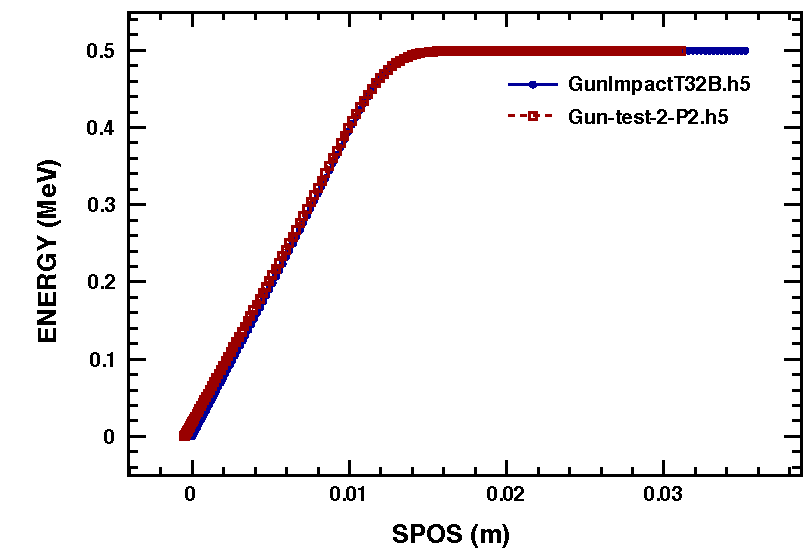
\includegraphics[width=0.6\linewidth,angle=90]{figures/Gun/GunCompEn}
%   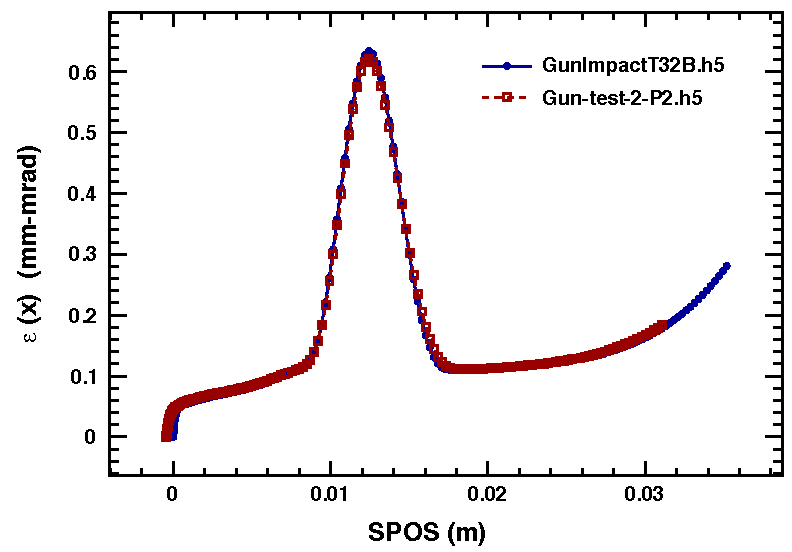
\includegraphics[width=0.6\linewidth,angle=90]{figures/Gun/GunCompEx}
%   \caption{Comparison of energy and emittance in $x$ between \impactt and \opalt}
%   \label{fig:guncomp2}
% \end{center}
%\end{figure}

\subsection{PSI XFEL 250 MeV Injector}
\label{sec:felinj}
\index{XFEL}
\index{INJECTOR}
\examplefromfile{examples/diagnostic.in}



\subsection{PSI  Injector II Cyclotron}
\label{sec:inj2}
\index{INJECTOR II}
\index{CYCLOTRON}
%%%%%%%%%%
Injector II is a separated sector cyclotron specially designed for pre-acceleration (inject: \SI{870}{\kilo\electronvolt}, extract: \SI{72}{\mega\electronvolt} )
of high intensity proton beam for Ring cyclotron. It has 4 sector magnets, two double-gap acceleration cavities
(represented by 2 single-gap cavities here) and two single-gap flat-top cavities.

Following is an input file of {\bfseries Single Particle Tracking mode} for PSI Injector II cyclotron.

\examplefromfile{examples/opal-cycl.in}

To run opal on a single node, just use this command:
\begin{example}
 opal testinj2-1.in
\end{example}

Here shows some pictures using the resulting data from single particle tracking using \opalcycl.

Left plot of \figref{Inj2 reference orbit and tune} shows the accelerating orbit of reference particle. After 106 turns, the energy increases from \SI{870}{\kilo\electronvolt} at the injection point to \SI{72.16}{\mega\electronvolt} at the deflection point.

%======================FIGURE===============================
\begin{figure}[tb]
\centering
   \includegraphics[width=0.45\textwidth]{figures/cyclotron/AEO_Injector2.png}
   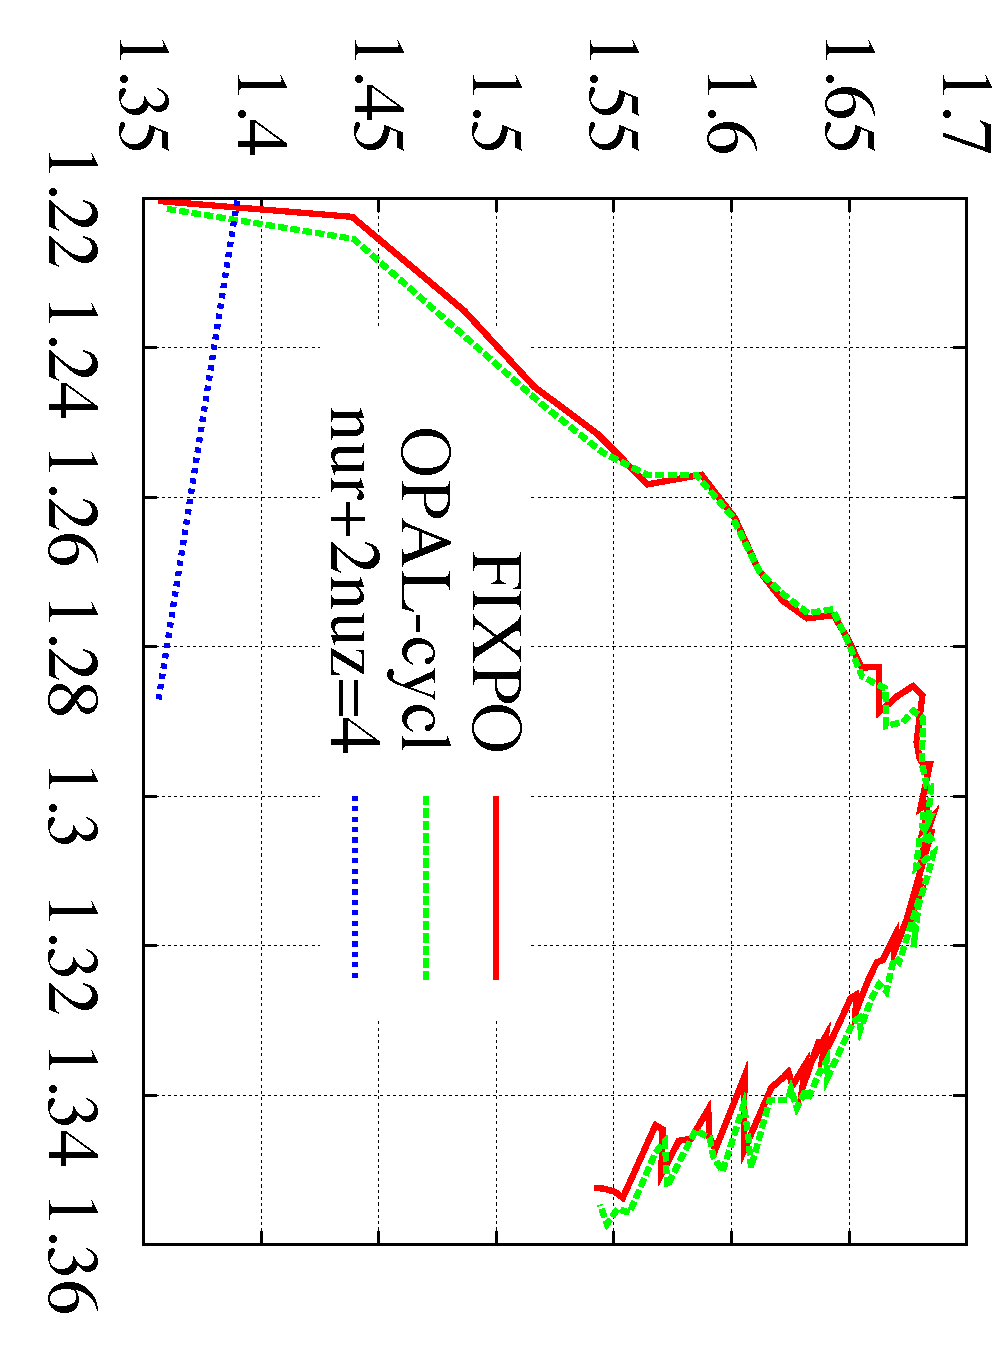
\includegraphics[width=0.40\textwidth,angle=90]{figures/cyclotron/nurnuz_Inj2}
   \caption{Reference orbit(left) and tune diagram(right) in Injector II  }
   \label{fig:Inj2 reference orbit and tune}
\end{figure}
%===========================================================


From theoretic view, there should be an eigen ellipse for any given energy in stable area of a fixed accelerator structure. Only when the initial phase space
shape matches its eigen ellipse, the oscillation of beam envelop amplitude will get minimal and the transmission efficiency get maximal.
We can calculate the eigen ellipse by single particle tracking using betatron oscillation property of off-centered particle as following: track
an off-centered particle and record its coordinates and momenta at the same azimuthal position for each revolution.
\figref{eigen} shows the eigen ellipse at symmetric line of sector magnet for energy of \SI{2}{\mega\electronvolt} in Injector II.

%======================FIGURE===============================
\begin{figure}[tb]
\centering
   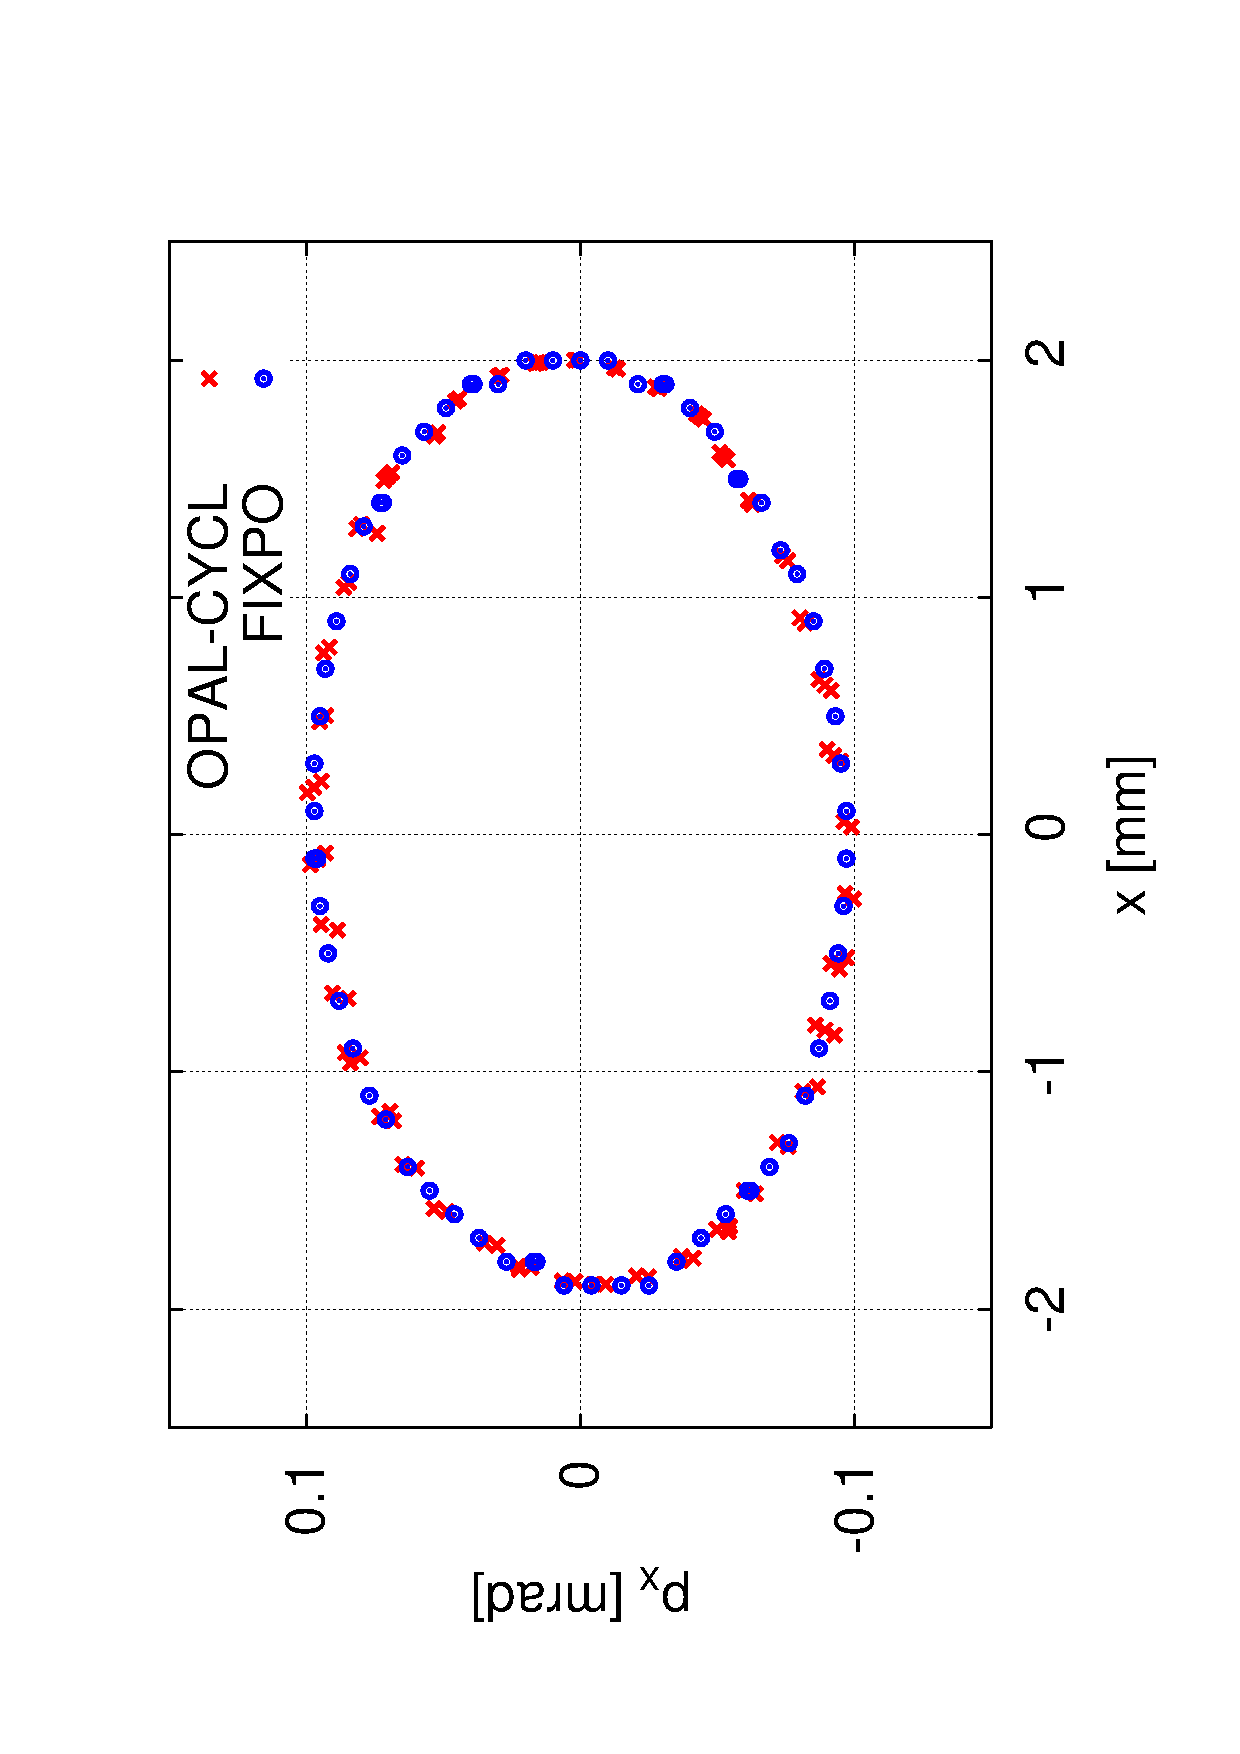
\includegraphics[width=0.45\textwidth]{figures/cyclotron/RadialEigen_Inj2}
   \includegraphics[width=0.45\textwidth]{figures/cyclotron/VertEigen_Inj2}
   \caption{Radial and vertical eigenellipse at \SI{2}{\mega\electronvolt} of Injector II}
   \label{fig:eigen}
\end{figure}
%===========================================================


Right plot of \figref{Inj2 reference orbit and tune} shows very good agreement of the tune diagram by \opalcycl and FIXPO.
The trivial discrepancy should come from the methods they used.
In FIXPO, the tune values are obtained according to the crossing points of the initially displaced particle. Meanwhile, in \opalcycl, the Fourier
analysis method is used to manipulate orbit difference between the reference particle and an initially displaced particle.
The frequency point with the biggest amplitude is the betatron tune value at the given energy.

%%%%%%%%%%%%%%
Following is the input file for single bunch tracking with space charge effects in Injector II.
%%%%%%%%%%%%%%

\examplefromfile{examples/opal-cycl-sc.in}

To run opal on single node, just use this command:
\begin{example}
 # opal testinj2-2.in
\end{example}

To run opal on N nodes in parallel environment interactively, use this command instead:
\begin{example}
 # mpirun -np N opal testinj2-2.in
\end{example}

If restart a job from the last step of an existing \filename{.h5} file, add a new argument like this:
\begin{example}
 # mpirun -np N opal testinj2-2.in -restart -1
\end{example}
\figref{cyclParameters,cyclphasespace} are simulation results, shown by  H5ROOT code.

%======================FIGURE===============================
\begin{figure}[tb]
\centering
    \includegraphics[width=0.45\textwidth]{figures/cyclotron/Inj2-ENERGY-TIME.png}
    \includegraphics[width=0.45\textwidth]{figures/cyclotron/Inj2-B-ref-z-TrackStep.png}
    \caption{Energy Vs. time (left) and external B field Vs. track step (Right, only show for about 2 turns)}
    \label{fig:cyclParameters}
\end{figure}
%===========================================================


%======================FIGURE===============================
\begin{figure}[tb]
\centering
    \includegraphics[width=0.3\textwidth]{figures/cyclotron/Inj2-z-pz-step-870KeV.png}
    \includegraphics[width=0.3\textwidth]{figures/cyclotron/Inj2-z-pz-step-15MeV.png}
    \includegraphics[width=0.3\textwidth]{figures/cyclotron/Inj2-z-pz-step-30MeV.png}
    \caption{Vertical phase at different energy from left to right: \SI{0.87}{\mega\electronvolt}, \SI{15}{\mega\electronvolt} and \SI{35}{\mega\electronvolt}}
    \label{fig:cyclphasespace}
\end{figure}
%===========================================================



%%%%%%%%%%%%%%
\subsection{PSI  Ring Cyclotron}
\label{sec:Ring}
\index{RING}
\index{CYCLOTRON}
From the view of numerical simulation, the difference between Injector II and Ring cyclotron comes from two aspects:
\begin{description}
\item[B Field] The structure of Ring is totally symmetric, the field on median plain is periodic
along azimuthal direction, \opalcycl take this advantage to only store \nicefrac{1}{8} field data to save memory.

\item[RF Cavity] In the Ring, all the cavities are typically single gap with some parallel displacement from its
radial position.\opalcycl have an argument \keyword{PDIS} to manipulate this issue.
\end{description}
\begin{figure}[ht]
  \begin{center}
    \includegraphics[width=6cm,trim=2.5cm 2.5cm 2.5cm 2.5cm]{figures/cyclotron/AEO_Ring.png}
    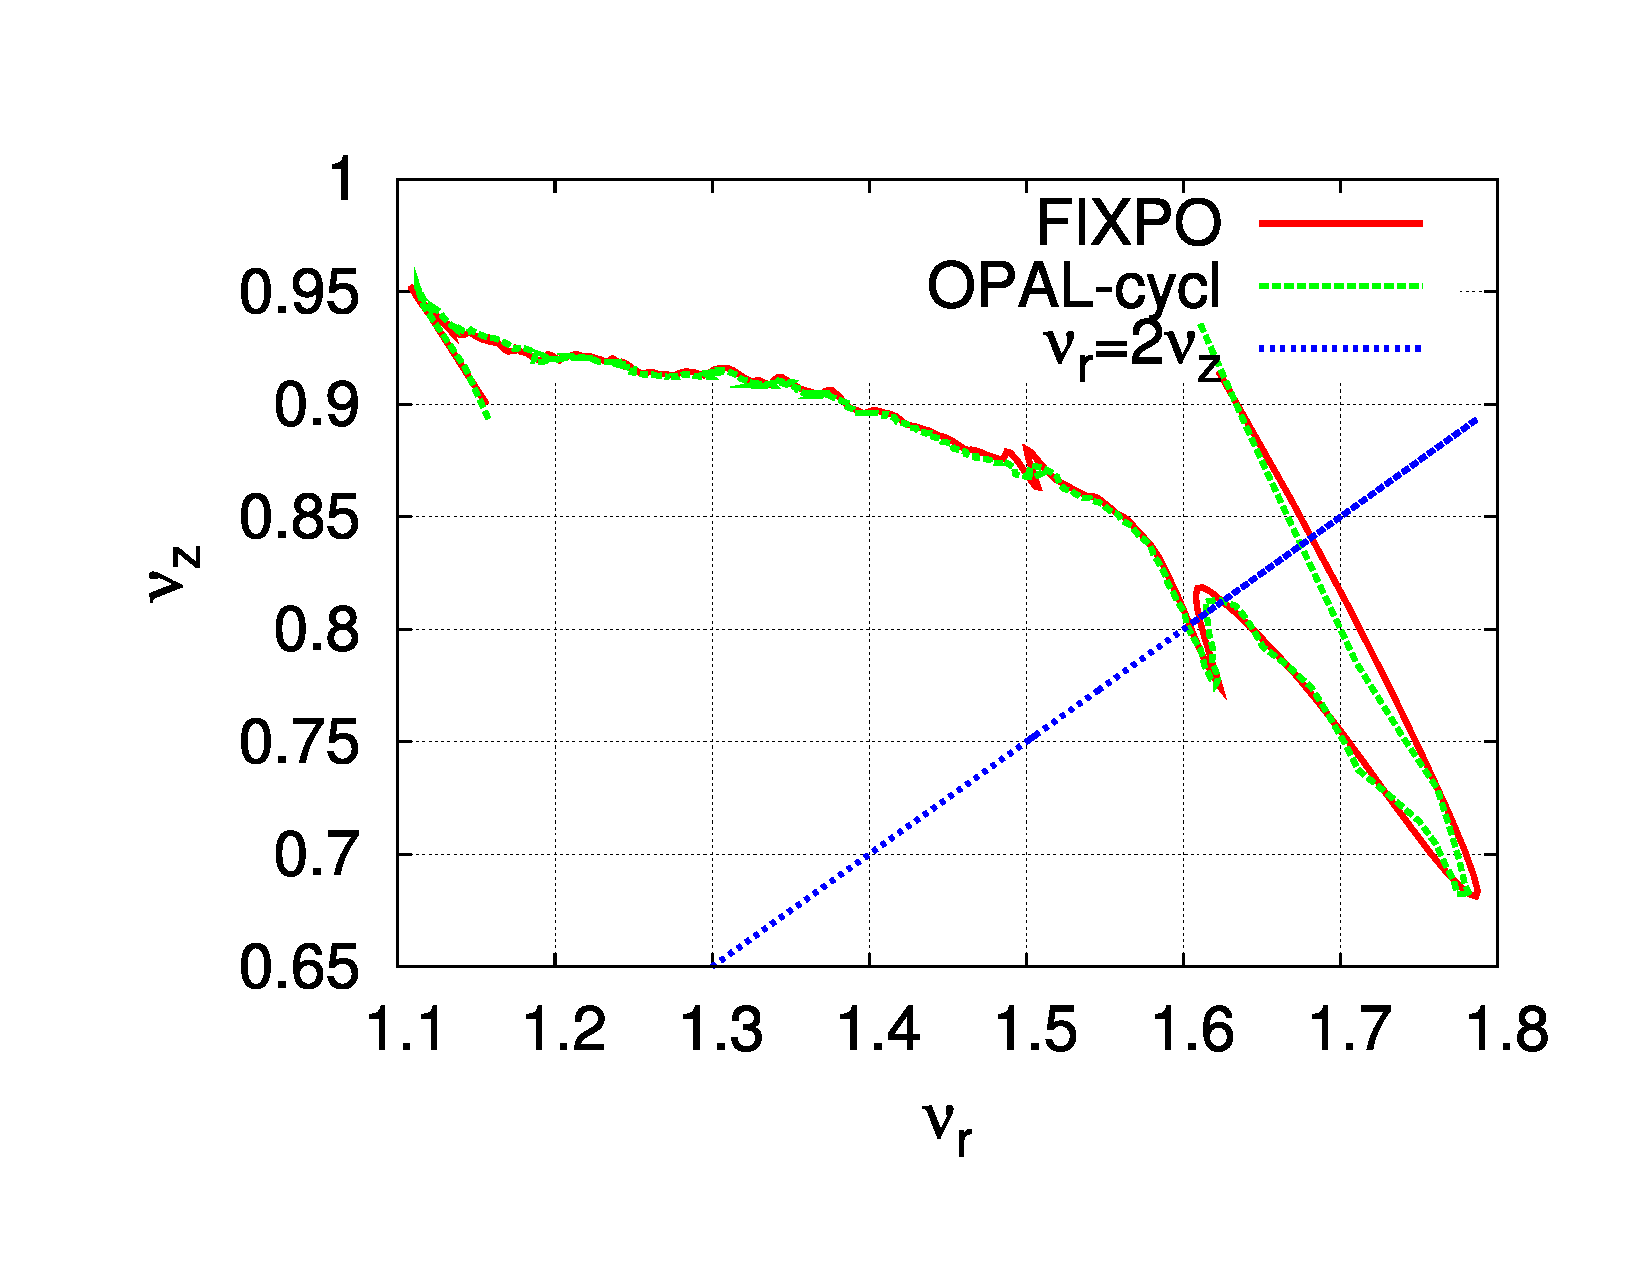
\includegraphics[width=6cm,trim=2.5cm 2.5cm 2.5cm 2.5cm]{figures/cyclotron/nurnuz_Ring}
    \caption{Reference orbit(left) and tune diagram(right) in Ring cyclotron }
    \label{fig:Ring reference orbit and tune}
  \end{center}
\end{figure}
\figref{Ring reference orbit and tune} shows a single particle tracking result and tune calculation result in the PSI Ring cyclotron.
Limited by size of the user guide, we don't plan to show too much details as in Injector II.

\clearpage


\section{Translate Old Distribution Commands to New Distribution Commands}
\label{sec:oldtonewdist}
\index{Distribution!Translate Old}
As of \opal 1.2, the distribution command \seechp{distribution} was changed significantly. Many of the changes were internal to the code, allowing us to more easily add new distribution command options. However, other changes were made to make creating a distribution easier, clearer and so that the command attributes were more consistent across distribution types. Therefore, we encourage our users to refer to \chpref{distribution} when creating any new input files, or if they wish to update existing input files.

With the new distribution command, we did attempt as much as possible to make it backward compatible so that existing \opal input files would still work the same as before, or with small modifications. In this section of the manual, we will give several examples of distribution commands that will still work as before, even though they have antiquated command attributes. We will also provide examples of commonly used distribution commands that need small modifications to work as they did before.

\textbf{\emph{An important point to note is that it is very likely you will see small changes in your simulation even when the new distribution command is nominally generating particles in exactly the same way.}} This is because random number generators and their seeds will likely not be the same as before. These changes are only due to \opal using a different sequence of numbers to create your distribution, and not because of errors in the calculation. (Or at least we hope not.)

\subsection{\keyword{GUNGAUSSFLATTOPTH} and \keyword{ASTRAFLATTOPTH} Distribution Types}
\label{sec:oldtonewdistgungaussandastra}
\index{Distribution!Translate GUNGAUSSFLATTOPTH}
\index{Distribution!Translate ASTRAFLATTOPTH}
The \keyword{GUNGAUSSFLATTOPTH} and \keyword{ASTRAFLATTOPTH} distribution types \seesec{gungaussflattopthdisttype,astraflattopthdisttype} are two common types previously implemented to simulate electron beams emitted from photocathodes in an electron photoinjector. These are no longer explicitly supported and are instead now defined as specialized sub-types of the distribution type \keyword{FLATTOP}. That is, the \emph{emitted} distributions represented by \keyword{GUNGAUSSFLATTOPTH} and \keyword{ASTRAFLATTOPTH} can now be easily reproduced by using the \keyword{FLATTOP} distribution type and we would encourage use of the new command structure.

Having said this, however, old input files that use the \keyword{GUNGAUSSFLATTOPTH} and \keyword{ASTRAFLATTOPTH} distribution types will still work as before, with the following exception. Previously, \opal had a Boolean \keyword{OPTION} command \keyword{FINEEMISSION} (default value was \keyword{TRUE}). This \keyword{OPTION} is no longer supported. Instead you will need to set the distribution attribute \keyword{EMISSIONSTEPS} \seetab{distattremitted} to a value that is 10 $\times$ the value of the distribution attribute \keyword{NBIN} \seetab{distattruniversal} in order for your simulation to behave the same as before.
%----------- Footer control ------------------
\ifthenelse{\boolean{FullOPALManual}}
{
  %do nothing
}
% else (for individual document creation)
{
\appendix
\printbibliography
\end{document}
}
%---------------------------------------------

\subsection{\keyword{FROMFILE}, \keyword{GAUSS} and \keyword{BINOMIAL} Distribution Types}
\index{Distribution!Translate FROMFILE}
\index{Distribution!Translate GAUSS}
\index{Distribution!Translate BINOMIAL}
The \keyword{FROMFILE} \seesec{fromfiledisttype}, \keyword{GAUSS} \seesec{gaussdisttype} and \keyword{BINOMIAL} \seesec{binomialdisttype} distribution types have changed from previous versions of \opal. However, legacy distribution commands should work as before with one exception. If you are using \opalcycl then your old input files will work just fine. However, if you are using \opalt then you will need to set the distribution attribute \keyword{INPUTMOUNITS} \seesec{unitsdistattributes} to:
\begin{example}
INPUTMOUNITS = EV
\end{example}              % ch 3
\ifdefined \buildingFullOPALManual \else


%\ifx \@buildingFullOPALManual \@empty
%\else

%\documentclass[12pt,a4paper]{report}
\documentclass[a4paper]{book}

%% does not work in Latex2Html mode
%\usepackage{hyperref}

\usepackage[T1]{fontenc}
\usepackage{url}
\usepackage{html}
\usepackage{epic}
\usepackage{eepic}
\usepackage{makeidx}
\usepackage{array}
\usepackage{times}
\usepackage{amsmath}
\usepackage{amsxtra}
\usepackage{bm}
\usepackage[thin,thinp,thinc]{esdiff}
\usepackage{etoolbox}
\usepackage{graphicx}
\usepackage{dingbat}
\usepackage{color}
\usepackage{subfig}
\usepackage{boxedminipage}
\usepackage{alltt}
\usepackage{nicefrac}
\usepackage{calc}
%\usepackage{pdfdraftcopy}             % Draft
\usepackage{tikz}
\usetikzlibrary{
  er,3d,calc,fadings,trees,positioning,arrows,chains,decorations.pathreplacing,
  decorations.pathmorphing,shapes,shapes.symbols,shapes.arrows,matrix,through,decorations.text
}

\tikzset{
  >=stealth',
  punktchain/.style={rectangle,rounded corners, draw=black, very thick,text width=10em,
                     minimum height=3em, text centered, on chain},
  line/.style={draw, thick, <-},
  element/.style={tape,top color=white,bottom color=blue!50!black!60!,minimum width=8em,
                  draw=blue!40!black!90, very thick,text width=10em, minimum height=3.5em,
                  text centered, on chain},
  every join/.style={->, thick,shorten >=1pt},
  tuborg/.style={decorate},
  tubnode/.style={midway, right=2pt}
}

\tikzstyle{material}=[draw, fill=blue!20, text width=16.0em, text centered, minimum height=1.5em]
\tikzstyle{diagramstep} = [material, text width=20em, minimum width=10em, minimum height=3em, rounded corners]
\tikzstyle{line} = [draw, thick, color=black!50, -latex']

\usepackage{booktabs}
\usepackage{xspace}
\usepackage{xstring}

\usepackage{fancyvrb}
\usepackage{rotating}
\usepackage{float}

\usepackage{tabularx}
\usepackage{longtable}
\setcounter{LTchunksize}{3}

\usepackage[section]{placeins}
\usepackage{MnSymbol}
\usepackage{microtype}
\usepackage{setspace}
\usepackage{dcolumn}

\usepackage[vmargin={3.0cm,3.0cm},
            hmargin={2.0cm,3.0cm}]{geometry}

\usepackage{upgreek}
\usepackage[binary-units=true]{siunitx}
\sisetup{exponent-product = \cdot,math-ohm=\Upomega,text-ohm=\ensuremath{\Upomega}}
\DeclareSIUnit{\clight}{c}
\DeclareSIUnit\gauss{Ga}

\usepackage{engord}
\usepackage{wasysym}
\DeclareSIUnit[number-unit-product = \,]{\permill}{\permil}

\usepackage{hyperref}
\hypersetup{
    pdftitle          = The OPAL Framework,
    pdfauthor         = {Andreas Adelmann, Achim Gsell, Valeria Rizzoglio, Christof Metzger-Kraus,
                         Yves Ineichen, Xiaoying Pang, Steve Russell, Chuan Wang, Jianjun Yang,
                         Suzanne Sheehy, Chris Rogers, Daniel Winklehner},
    pdfsubject        = User's Reference Manual,
    pdffitwindow      = true,               % page fit to window when opened
    pdfnewwindow      = true,               % links in new window
    colorlinks        = true,               % false: boxed links; true: colored links
    linkcolor         = black!80!green,     % color of internal links
    citecolor         = black!20!red,       % color of links to bibliography
    urlcolor          = blue,               % color of external links
    breaklinks        = true,
    bookmarksnumbered = true,
    plainpages        = false
}

\usepackage{ifthen}

\newif \iflinuxwindows
\linuxwindowstrue   % set this to true when building the manual on Linux or Windows
\iflinuxwindows
\usepackage{epstopdf}
\fi

\usepackage[backend=biber,
            style=phys,
            biblabel=brackets,
            maxnames=3,
            doi=true,
            isbn=true,
            url=true]{biblatex}
%---- macros ----

\renewcommand{\topfraction}{1.0}
\renewcommand{\bottomfraction}{1.0}
\renewcommand{\textfraction}{0.0}
\renewcommand{\arraystretch}{2.0}
\newenvironment{tex2html_nowrap}{}{}


\newcommand{\Newline}{\hfil \\}


\newsavebox{\ExampleBox}
\newenvironment{example}
 {\VerbatimEnvironment
  \begin{flushleft}
  \begin{lrbox}{\ExampleBox}
    \begin{minipage}{\linewidth}
  \begin{Verbatim}[frame=lines,xleftmargin=0cm,fontsize=\footnotesize,samepage=true]}
 {\end{Verbatim}
  \end{minipage}
  \end{lrbox}
  \mbox{\usebox{\ExampleBox}}
  \end{flushleft}
 }

\newenvironment{longexample}
{\Verbatim[frame=lines,xleftmargin=0mm,fontsize=\footnotesize]}
{\endVerbatim}

%\examplefromfile{filename} reads in a text file and displays it in the document.
\newcommand{\examplefromfile}[1]{
\VerbatimInput[frame=lines,xleftmargin=0mm,fontsize=\footnotesize,label=\texttt{#1}]{#1}}

%for upright d of differentials
\makeatletter
\newcount\my@repeat@count

\newcommand{\myrepeat}[2]{%
  \begingroup
  \my@repeat@count=\z@
  \@whilenum\my@repeat@count<#1\do{#2\advance\my@repeat@count\@ne}%
  \endgroup
}

\newcommand{\differential}[1]{\ifstrempty{#1}{\ES@dop\ES@difint}{\ES@dop^{#1}\ES@difint}}
\newcommand{\pdifferential}[1]{\ifstrempty{#1}{{\partial\,}}{{\partial^{#1}\,}}}

\makeatother

\newcommand{\der}[3][]{\frac{\differential{#1}#2}{\differential{}\ifstrempty{#1}{#3}{#3^#1}}}
\newcommand{\parder}[3][]{\frac{\pdifferential{#1}#2}{\pdifferential{}\ifstrempty{#1}{#3}{#3^#1}}}
\newcommand{\niceder}[3][]{\nicefrac{\differential{#1}#2}{\differential{}\ifstrempty{#1}{#3}{#3^#1}}}
\newcommand{\uglyder}[3][]{{\differential{#1}#2}/{\differential{}\ifstrempty{#1}{#3}{#3^#1}}}
\newcommand{\uglyparder}[3][]{{\pdifferential{#1}#2}/{\pdifferential{}\ifstrempty{#1}{#3}{#3^#1}}}
\newcommand{\dd}[1][]{\; \differential{#1}}
\newcommand{\primed}{^{\prime}}
\newcommand{\dprimed}{^{\prime\prime}}
\newcommand{\nprimed}[1]{^{\myrepeat{#1}{\prime}}}

%Editing Macros
\newcommand{\TODO}[1]{{\color{red}\ifthenelse{\boolean{ShowDebug}}{[TODO: #1]}{}}}



%text in gray box
\newsavebox{\fmbox}
\definecolor{lightgray}{gray}{0.95}
\newenvironment{fmpage}
   {\vspace{-1.0cm}\begin{lrbox}{\fmbox}\begin{minipage}[t]{13.5cm}\vspace{0.1cm}}
   {\vspace{-0.4cm}\end{minipage}\end{lrbox}\begin{center}\fcolorbox{black}{lightgray}{\usebox{\fmbox}}\end{center}}


% Definition new signes
\newcommand{\R}{{\mathbb R}} % real numbers
\newcommand{\Q}{{\mathbb Q}} % rational numbers
\newcommand{\Z}{{\mathbb Z}} % integer numbers
\newcommand{\N}{{\mathbb N}} % natural numbers

\newcommand{\mad}{\textsc{mad}\xspace}
\newcommand{\madnine}{\textsc{mad9}\xspace}
\newcommand{\madninep}{\textsc{mad9p}\xspace}
\newcommand{\madeight}{\textsc{mad8}\xspace}
\newcommand{\classic}{\textsc{classic}\xspace}

\makeatletter
\newcommand{\opal@impl}{\textsc{Opal}}
\newcommand{\opalt@impl}{\textsc{Opal-t}}
\newcommand{\opalcycl@impl}{\textsc{Opal-cycl}}
\newcommand{\opalmap@impl}{\textsc{Opal-map}}
\newcommand{\opalenv@impl}{\textsc{Opal-e}}

\newcommand{\opal}{\opal@impl\xspace}
\newcommand{\opalt}{\opalt@impl\xspace}
\newcommand{\opalcycl}{\opalcycl@impl\xspace}
\newcommand{\opalmap}{\opalmap@impl\xspace}
\newcommand{\opalenv}{\opalenv@impl\xspace}

\newcommand{\noopalt}{\leftthumbsdown \opalt@impl\xspace}
\newcommand{\noopalcycl}{\leftthumbsdown \opalcycl@impl\xspace}
\newcommand{\noopalmap}{\leftthumbsdown \opalmap@impl\xspace}
\newcommand{\noopalenv}{\leftthumbsdown \opalenv@impl\xspace}
\makeatother

\newcommand{\impactt}{\textsc{Impact-t}\xspace}
\newcommand{\partroot}{\textsc{H5root}}


\newcommand{\latermore}{More details will be given in Version 1.6.0}


\newcommand{\lieop}[1]{{:}{#1}{:}}

\newcommand{\rms}[1]{\overset{\sim}{#1}}

\newcommand{\sprod}{\cdot}
\newcommand{\vprod}{\times}
\newcommand{\matr}[1]{\mathcal{#1}}
\renewcommand{\vec}[1]{{\bm{#1}}}
\newcommand{\transpose}[1]{#1^\intercal}
\renewcommand{\epsilon}{\varepsilon}

\newcommand{\keyword}[2][]{\ifstrempty{#1}{\texttt{\expandafter\MakeUppercase\expandafter{#2}}}{\hyperref[#1]{\texttt{\expandafter\MakeUppercase\expandafter{#2}}}}}
\newcommand{\tabline}[3][]{\keyword[#1]{#2}& #3 \\}
\newcommand{\tabheadcell}[1]{{\bfseries #1}}

\newcommand*\kdescriptionlabel[1]{\hspace\labelsep
                                \normalfont\keyword{#1}\index{#1}}
\makeatletter
\newenvironment{kdescription}
               {\list{}{\labelwidth\z@ \itemindent-\leftmargin
                        \let\makelabel\kdescriptionlabel}}
               {\endlist}
\makeatother

\ExplSyntaxOn
\NewDocumentCommand{\tabhead}{ m }
 {
  \seq_set_split:Nnn \l_tmpa_seq { & } { #1 }
  \bfseries \seq_use:Nn \l_tmpa_seq { & \bfseries } \\
 }

\NewDocumentCommand \multrefImpl { O{ } m m m } {
  \ifnumgreater{\clist_count:n {#4}}{1}{
    \seq_set_from_clist:Nn \l_tmpa_seq { #4 }

    \seq_set_map:NNn \l_tmpb_seq \l_tmpa_seq { \exp_not:n { \ref{#3:##1} } }
    \ifstrempty{#1}{#2s}{#1}~\seq_use:Nnnn \l_tmpb_seq {\ and\ } {,\ } {,\ and\ }
  }{
    #2~\ref{#3:#4}
  }
}

\NewDocumentCommand \multeqnrefImpl { m } {
  \ifnumgreater{\clist_count:n {#1}}{1}{
    \seq_set_from_clist:Nn \l_tmpa_seq { #1 }

    \seq_set_map:NNn \l_tmpb_seq \l_tmpa_seq { \exp_not:n { \eqref{eq:##1} } }
    Equations~\seq_use:Nnnn \l_tmpb_seq {\ and\ } {,\ } {,\ and\ }
  }{
    Equation~\eqref{eq:#1}
  }
}
\ExplSyntaxOff


%Abbreviations for Equations, Figures, and Tables
%\newcommand{\Equation}[1]{Equation~\eqref{#1}}

\newcommand{\bibref}[2]{#1 \cite{bib:#2}}
\newcommand{\figref}[1]{\multrefImpl{Figure}{fig}{#1}}
\newcommand{\chpref}[1]{\multrefImpl{Chapter}{chp}{#1}}
\newcommand{\appref}[1]{\multrefImpl[Appendices]{Appendix}{chp}{#1}}
\newcommand{\secref}[1]{\multrefImpl{Section}{sec}{#1}}
\newcommand{\ssecref}[1]{\multrefImpl{Section}{ssec}{#1}}
\newcommand{\tabref}[1]{\multrefImpl{Table}{tab}{#1}}
\newcommand{\eqnref}[1]{\multeqnrefImpl{#1}}

\newcommand{\seefig}[1]{(see~\figref{#1})}
\newcommand{\seechp}[1]{(see~\chpref{#1})}
\newcommand{\seesec}[1]{(see~\secref{#1})}
\newcommand{\seessec}[1]{(see~\ssecref{#1})}
\newcommand{\seetab}[1]{(see~\tabref{#1})}
\newcommand{\seeeqn}[1]{(see~\eqnref{#1})}

\newcommand{\filename}[1]{\emph{#1}}


% Define distances for bordering
\newcommand{\blockdist}{1.3}
\newcommand{\edgedist}{1.5}
\newcommand{\diagramstep}[2]{node (p#1) [diagramstep] {#2}}


% place chapter title page on odd pages
\let\stdchapter\chapter
\makeatletter
\renewcommand*{\chapter}{\if@openright\cleardoublepage\else\clearpage\fi\stdchapter}

\makeatother

\IfFileExists{./version.tex}{%
  \input{version}%
}%
{%
  \input{noversion}%
}
\newboolean{ShowMap}
\setboolean{ShowMap}{false}

\newboolean{ShowEnv}
\setboolean{ShowEnv}{false}

\newboolean{ShowDebug}
\setboolean{ShowDebug}{false}

%----Control Structures
\newboolean{FullOPALManual}
\setboolean{FullOPALManual}{false}


\makeindex


\bibliography{bibliography}
\begin{document}

\fi

\chapter{\opalt}
\label{chp:opalt}
\index{OPAL-t}
\index{PARALLEL-T}
\section{Introduction}
\opalt is a fully three-dimensional program to track in time, relativistic particles taking into account space charge forces, self-consistently in the electrostatic approximation, and short-range longitudinal and transverse wake fields. \opalt is one of the few
codes  that is implemented using a parallel programming paradigm from the ground up. This makes \opalt indispensable for
high statistics simulations of various kinds of existing and new accelerators. It has a comprehensive set of beamline
elements, and furthermore allows arbitrary overlap of their fields, which gives \opalt a capability
to model both the standing wave structure and traveling wave structure. Beside IMPACT-T it is the only code making use of
space charge solvers based on an integrated Green \cite{qiang2005, qiang2006-1,qiang2006-2} function to efficiently and accurately treat beams with
large aspect ratio, and a shifted Green function to efficiently treat image charge effects of a cathode \cite{fubiani2006, qiang2005, qiang2006-1,qiang2006-2}.
For simulations of particles sources i.e. electron guns \opalt uses the technique of  energy binning in the electrostatic space charge calculation to model beams with large
energy spread. In the very near future a parallel Multigrid solver taking into account the exact geometry will be implemented.

\section{Variables in \opalt}
\label{sec:variablesopalt}
\index{OPAL-t!Variables}

\label{sec:opalt:canon}
\index{Canonical Variables}
\index{Variables!Canonical}
\opalt uses the following canonical variables
to describe the motion of particles. The physical units are listed in square brackets.

\begin{description}
\item[X]
  Horizontal position $x$ of a particle relative to the axis of the element [m].

\item[PX]
  $\beta_x\gamma$ Horizontal canonical momentum [1].

\item[Y]
  Horizontal position $y$ of a particle relative to the axis of the element [m].

\item[PY]
  $\beta_y\gamma$ Horizontal canonical momentum [1].

\item[Z]
  Longitudinal position $z$ of a particle in floor co-ordinates [m].

\item[PZ]
 $\beta_z\gamma$ Longitudinal canonical momentum [1].

 \end{description}

The independent variable is  \textbf{t} [s].



\section{Integration of the Equation of Motion}
\opalt integrates the relativistic Lorentz equation
\begin{equation} \diff{\gamma\vec{v}}{t}
 =   \frac{q}{m}[\vec{E}_{ext} + \vec{E}_{sc} + \vec{v} \times (\vec{B}_{ext} + \vec{B}_{sc})]
\end{equation}
where $\gamma$ is the relativistic factor, $q$ is the charge, and $m$ is the rest mass of the particle. $\vec{E}$  and $\vec{B}$ are abbreviations for the electric field $\vec{E}(\vec{x},t)$ and  magnetic field $\vec{B}(\vec{x},t)$. To update the positions and momenta \opalt uses the Boris-Buneman algorithm \cite{langdon}.


\section{Positioning of Elements}
Since \opalversion{2.0} of \opal elements can be placed in space using 3D coordinates \keyword{X}, \keyword{Y}, \keyword{Z}, \keyword{THETA}, \keyword{PHI} and \keyword{PSI}, see \secref{Element:common}. The old notation using \keyword{ELEMEDGE} is still supported. \opalt then computes the position in 3D using \keyword{ELEMDGE}, \keyword{ANGLE} and \keyword{DESIGNENERGY}. It assumes that the trajectory consists of straight lines and segments of circles. Fringe fields are ignored. For cases where these simplifications aren't justifiable the user should use 3D positioning. For a simple switchover \opal writes a file \filename{\_3D.opal} where all elements are placed in 3D.

Beamlines containing guns should be supplemented with the element \keyword[sec:source]{SOURCE}. This allows \opal to distinguish the cases and adjust the initial energy of the reference particle.

Prior to \opalversion{2.0} elements needed only a defined length. The transverse extent was not defined for elements except when combined with 2D or 3D field maps. An aperture had to be designed to give elements a limited extent in transverse direction since elements now can be placed freely in three-dimensional space. See \secref{Element:common} for how to define an aperture.
\section{Coordinate Systems}
\label{sec:CoordinateSystems}
The motion of a charged particle in an accelerator can be described by relativistic Hamilton mechanics.
A particular motion is that of the reference particle, having the central energy and traveling on the
so-called reference trajectory. Motion of a particle close to this fictitious reference particle
can be described by linearized equations for the displacement of the particle under study, relative to the
reference particle. In \opalt, the time $t$ is used as independent variable instead of the path length $s$. The relation between them can be expressed as
\begin{equation}
\frac{\differential{}}{\differential{} t} = \frac{\differential{}}{\differential{}\vec{s}}\frac{\differential{}\vec{s}}{\differential{} t} = \vec{\beta}c\frac{\differential{}}{\differential{}\vec{s}}.
\end{equation}
\subsubsection{Global Cartesian Coordinate System}
We define the global cartesian coordinate system, also known as floor coordinate system with $K$, a point in this coordinate system is denoted by $(X, Y, Z) \in K$.
In \figref{KS1} of the accelerator is uniquely defined by the sequence of physical elements in $K$.
The beam elements are numbered $e_0, \ldots , e_i, \ldots e_n$.
\begin{figure}[!htb]
\begin{center}
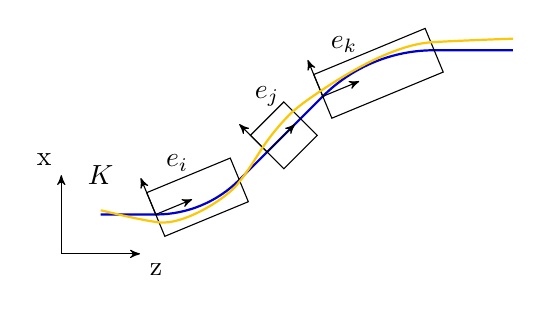
\begin{tikzpicture}
\draw[<->] (0,1cm) |- (1cm, 0);
\node[anchor=north west] at (1cm,0) {z};
\node[anchor=south east] at (0,1cm) {x};
\node at (0.5cm, 1cm) {$K$};
\draw[color=blue!80!black,thick] (0.5cm,0.5cm) -- (1.2cm,0.5cm) arc (270:315:1.5cm) -- ++(45:1.5cm) arc (135:90:2cm) --++(0:1cm);
\begin{scope}[cm={0.9239,0.3827,-0.3827,0.9239,(1.2cm,0.5cm)}]
    \draw (0,-0.3cm) rectangle (1.148cm,0.3cm);
    \draw[<->] (0.5cm,0)-|(0,0.5cm);
    \node at (0.5cm, 0.5cm) {$e_i$};
\end{scope}
\begin{scope}[cm={0.7071,0.7071,-0.7071,0.7071,(2.6142,1.2929)}]
    \draw (0,-0.3cm) rectangle (0.6cm,0.3cm);
    \draw[<->] (0.5cm,0)-|(0,0.5cm);
    \node at (0.5cm, 0.5cm) {$e_j$};
\end{scope}
\begin{scope}[cm={0.9239,0.3827,-0.3827,0.9239,(3.3213cm,2cm)}]
    \draw (0,-0.3cm) rectangle (1.5307cm,0.3cm);
    \draw[<->] (0.5cm,0)-|(0,0.5cm);
    \node at (0.5cm, 0.5cm) {$e_k$};
\end{scope}
\path[cm={2.849,0,0,2.849,(-8.4571,25.7235)},draw=yellow!80!red,line width=0.800pt]
  (3.144,-8.835) .. controls
  (3.144,-8.833) and (3.286,-8.872) .. (3.398,-8.888) .. controls
  (3.511,-8.905) and (3.705,-8.782) .. (3.755,-8.717) .. controls
  (3.801,-8.659) and (3.820,-8.626) .. (3.867,-8.553) .. controls
  (3.896,-8.509) and (3.955,-8.436) .. (3.999,-8.396) .. controls
  (4.044,-8.357) and (4.066,-8.343) .. (4.127,-8.301) .. controls
  (4.190,-8.260) and (4.427,-8.100) .. (4.615,-8.086) .. controls
  (4.689,-8.081) and (4.906,-8.072) .. (4.983,-8.070);
\end{tikzpicture}
  \caption{Illustration of local and global coordinates.}
  \label{fig:KS1}
\end{center}
\end{figure}

\subsubsection{Local Cartesian Coordinate System}
A local coordinate system $K'_i$ is attached to each element $e_i$. This is simply a frame in which $(0,0,0)$ is at the entrance of  each element. For an illustration see \figref{KS1}. The local reference system $(x, y, z) \in K'_n$
may thus be referred to a global Cartesian coordinate system $(X, Y, Z) \in K$.

The local coordinates $(x_i, y_i, z_i)$ at element $e_i$ with respect to the global coordinates $(X, Y, Z)$ are defined by three displacements $(X_i, Y_i, Z_i)$ and three angles $(\Theta_i, \Phi_i, \Psi_i)$.

$\Psi$ is the roll angle about the global $Z$-axis. $\Phi$ is the pitch angle about the global $Y$-axis. Lastly, $\Theta$ is the yaw angle about the global $X$-axis. All three angles form right-handed screws with their corresponding axes. The angles ($\Theta,\Phi,\Psi$) are the  Tait-Bryan angles \cite{bib:tait-bryan}.

The displacement is described by a vector $\vec{v}$
and the orientation by a unitary matrix $\matr{W}$.
The column vectors of $\matr{W}$ are unit vectors spanning
the local coordinate axes in the order $(x, y, z)$.
$\vec{v}$ and $\matr{W}$ have the values:
\begin{equation}
\vec{v} =\left(\begin{array}{c}
    X \\
    Y \\
    Z
  \end{array}\right),
\qquad
\matr{W}=\matr{S}\matr{T}\matr{U}
\end{equation}
where
\begin{equation}
\matr{S}=\left(\begin{array}{ccc}
    \cos\Theta &  0 &  \sin\Theta \\
    0         &  1 &   0 \\
    -\sin\Theta &  0 &  \cos\Theta
  \end{array}\right),
\quad
\matr{T}=\left(\begin{array}{ccc}
    1 &  0        &  0 \\
    0 &  \cos\Phi &  \sin\Phi \\
    0 & -\sin\Phi &  \cos\Phi
  \end{array}\right),
\end{equation}
\begin{equation}
\matr{U}=\left(\begin{array}{ccc}
    \cos\Psi & -\sin\Psi &  0 \\
    \sin\Psi &  \cos\Psi &  0 \\
    0        &  0        &  1
  \end{array}\right).
\end{equation}


We take the vector $\vec{r}_i$ to be the displacement and the matrix
$\matr{S}_i$ to be the rotation of the local reference system
at the exit of the element $i$ with respect to the entrance
of that element.

Denoting with $i$ a beam line element,
one can compute $\vec{v}_i$ and $\matr{W}_i$
by the recurrence relations
\begin{equation} \label{eq:surv}
\vec{v}_i = \matr{W}_{i-1}\vec{r}_i + \vec{v}_{i-1}, \qquad
\matr{W}_i = \matr{W}_{i-1}\matr{S}_i,
\end{equation}
where $\vec{v}_0$ corresponds to the origin of the \keyword{LINE} and $\matr{W}_0$ to its orientation. In \opalt they can be defined using either \keyword{X}, \keyword{Y}, \keyword{Z}, \keyword{THETA}, \keyword{PHI} and \keyword{PSI} or \keyword{ORIGIN} and \keyword{ORIENTATION}, see \secref{line:simple}.

\subsubsection{Space Charge Coordinate System}
In order to calculate space charge in the electrostatic approximation, we introduce a co-moving coordinate system $K_{\text{sc}}$, in which the origin coincides with the mean position of the particles and the mean momentum is parallel to the z-axis.


\subsubsection{Curvilinear Coordinate System}
In order to compute statistics of the particle ensemble, $K_s$ is introduced.
The accompanying tripod (Dreibein) of the reference orbit spans
a local curvilinear right handed system $(x,y,s)$.
The local $s$-axis is the tangent to the reference orbit.
The two other axes are perpendicular to the reference orbit and
are labelled~$x$ (in the bend plane)
and~$y$ (perpendicular to the bend plane).
\begin{figure}[!htb]
\begin{center}
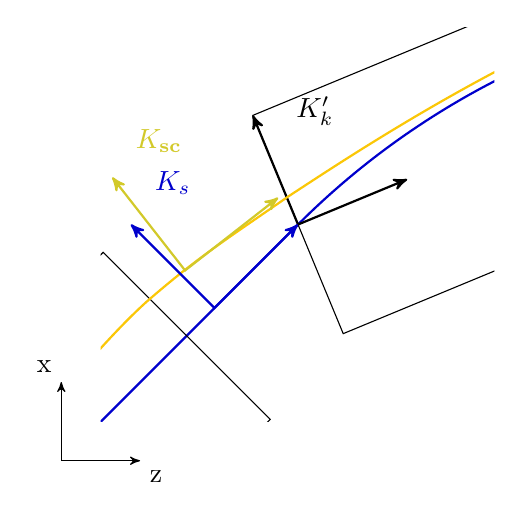
\begin{tikzpicture}
\draw[<->] (0,1cm) |- (1cm, 0);
\node[anchor=north west] at (1cm,0) {z};
\node[anchor=south east] at (0,1cm) {x};
\begin{scope}[cm={5,0,0,5,(-13.6,-7)}]
\begin{scope}
\clip (2.82,1.5) rectangle (3.82,2.5);
\draw[color=blue!80!black,thick] (0.5cm,0.5cm) -- (1.2cm,0.5cm) arc (270:315:1.5cm) -- ++(45:1.5cm) arc (135:90:2cm) --++(0:1cm);
\begin{scope}[cm={0.9239,0.3827,-0.3827,0.9239,(1.2cm,0.5cm)}]
    \draw (0,-0.3cm) rectangle (1.148cm,0.3cm);
%    \draw[<->] (0.5cm,0)-|(0,0.5cm);
    \node at (0.5cm, 0.5cm) {$e_i$};
\end{scope}
\begin{scope}[cm={0.7071,0.7071,-0.7071,0.7071,(2.6142,1.2929)}]
    \draw (0,-0.3cm) rectangle (0.6cm,0.3cm);
%    \draw[<->] (0.5cm,0)-|(0,0.5cm);
    \node at (0.5cm, 0.5cm) {$e_j$};
\end{scope}
\begin{scope}[cm={0.9239,0.3827,-0.3827,0.9239,(3.3213cm,2cm)}]
    \draw (0,-0.3cm) rectangle (1.5307cm,0.3cm);
    \draw[<->,thick] (0.3cm,0)-|(0,0.3cm);
    \node at (0.15cm, 0.25cm) {$K\primed_k$};
\end{scope}
\path[cm={2.849,0,0,2.849,(-8.4571,25.7235)},draw=yellow!80!red,line width=0.800pt]
  (3.144,-8.835) .. controls
  (3.144,-8.833) and (3.286,-8.872) .. (3.398,-8.888) .. controls
  (3.511,-8.905) and (3.705,-8.782) .. (3.755,-8.717) .. controls
  (3.801,-8.659) and (3.820,-8.626) .. (3.867,-8.553) .. controls
  (3.896,-8.509) and (3.955,-8.436) .. (3.999,-8.396) .. controls
  (4.044,-8.357) and (4.066,-8.343) .. (4.127,-8.301) .. controls
  (4.190,-8.260) and (4.427,-8.100) .. (4.615,-8.086) .. controls
  (4.689,-8.081) and (4.906,-8.072) .. (4.983,-8.070);
\end{scope}
\begin{scope}[cm={0.7071,0.7071,-0.7071,0.7071,(3.109,1.788)}]
\draw[<->,blue!80!black,thick] (0.3,0.0) -| (0.0,0.3);
\node[blue!80!black] at (0.15cm, 0.3cm) {$K_s$};
\end{scope}
\begin{scope}[cm={0.788,0.616,-0.616,0.788,(3.109,1.788)}]
\draw[<->,yellow!80!black,thick] (0.3,0.121) -| (0.0,0.421);
\node[yellow!80!black] at (0.15cm, 0.421cm) {\textbf{$K_{\text{sc}}$}};
\end{scope}
\end{scope}
\end{tikzpicture}
  \caption{Illustration of $K_\text{sc}$ and $K_s$}
  \label{fig:KS2}
\end{center}
\end{figure}
Both coordinate systems are described in \figref{KS2}.

\subsection{Design or Reference Orbit}
The reference orbit consists of a series of straight sections and circular arcs and is {\bf computed} by the Orbit Threader i.e. deduced from the element placement in the floor coordinate system.

\subsection{Compatibility Mode}
To facilitate the change for users we will provide a compatibility mode. The idea is that the user does not have to change the input file. Instead \opalt will compute the positions of the elements. For this it uses the bend angle and chord length of the dipoles and the position of the elements along the trajectory. The user can choose whether effects due to fringe fields are considered when computing the path length of dipoles or not. The option to toggle \opalt's behavior is called \keyword{IDEALIZED}. \opalt assumes per default that provided \keyword{ELEMEDGE} for elements downstream of a dipole are computed without any effects due to fringe fields.

Elements that overlap with the fields of a dipole have to be handled separately by the user to position them in 3D.

We split the positioning of the elements into two steps. In a first step we compute the positions of the dipoles. Here we assume that their fields don't overlap. In a second step we can then compute the positions and orientations of all other elements.

The accuracy of this method is good for all elements except for those that overlap with the field of a dipole.

\subsection{Orbit Threader and Autophasing}
\label{sec:orbitthreader}
The \texttt{OrbitThreader} integrates a design particle through the lattice and setups up a multi map structure (\texttt{IndexMap}). Furthermore when the reference particle hits an rf-structure for the first time then it auto-phases the rf-structure, see \appref{autophasing}. The multi map structure speeds up the search for elements that influence the particles at a given position in 3D space by minimizing the looping over elements when integrating an ensemble of particles. For each time step, \texttt{IndexMap} returns a set of elements $\mathcal{S}_{\text{e}} \subset {e_0 \ldots e_n}$ in case of the example given in \figref{KS1}. An implicit drift is modelled as an empty set $\emptyset$.

\subsection{Flow Diagram of \opalt}
\begin{figure}[!htb]
  \centering
 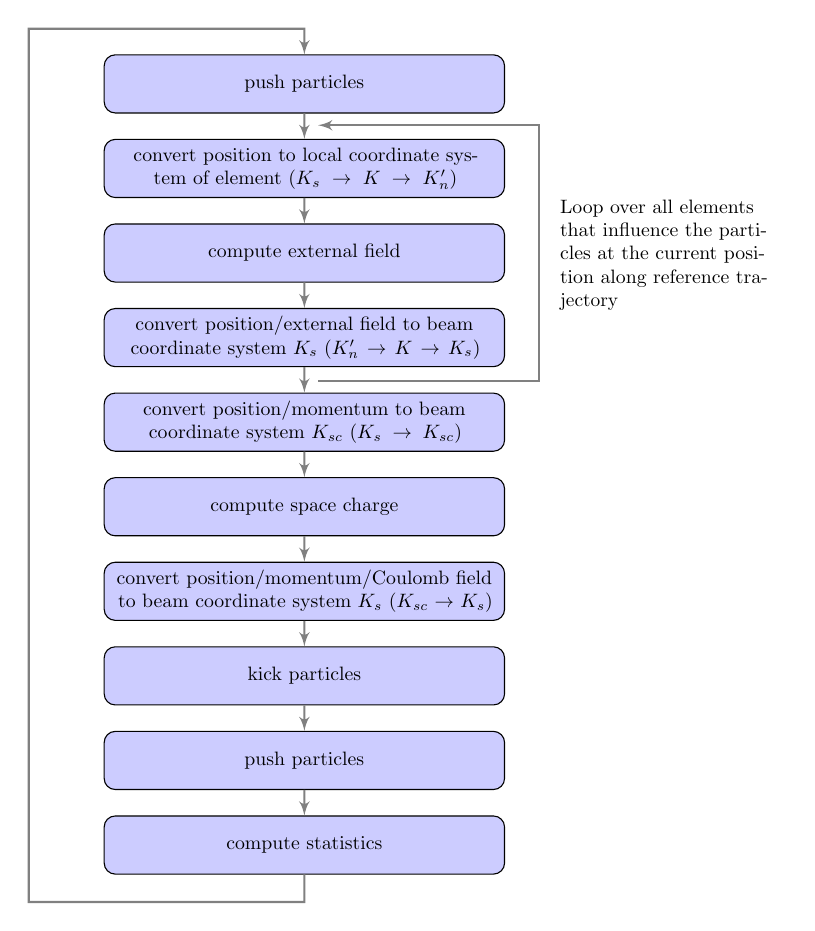
\begin{tikzpicture}[scale=0.7,transform shape]

  % Draw diagram elements
  \path \diagramstep {1}{push particles};
  \path (p1.south)+(0.0,-1.0) \diagramstep{2}{convert position to local coordinate system of element ($K_s \rightarrow K \rightarrow K'_n$)};
  \path (p2.south)+(0.0,-1.0) \diagramstep{3}{compute external field};
  \path (p3.south)+(0.0,-1.0) \diagramstep{4}{convert position/external field to beam coordinate system $K_s$ ($K'_n \rightarrow K \rightarrow K_s$)};
  \path (p4.south)+(0.0,-1.0) \diagramstep{5}{convert position/momentum to beam coordinate system $K_{sc}$ ($K_s \rightarrow K_{sc}$)};
  \path (p5.south)+(0.0,-1.0) \diagramstep{6}{compute space charge};
  \path (p6.south)+(0.0,-1.0) \diagramstep{7}{convert position/momentum/Coulomb field to beam coordinate system $K_s$ ($K_{sc} \rightarrow K_s$)};
  \path (p7.south)+(0.0,-1.0) \diagramstep{8}{kick particles};
  \path (p8.south)+(0.0,-1.0) \diagramstep{9}{push particles};
  \path (p9.south)+(0.0,-1.0) \diagramstep{11}{compute statistics};

  % Draw arrows between elements
  \path [line] (p1.south) -- node [above] {} (p2);
  \path [line] (p2.south) -- node [above] {} (p3);
  \path [line] (p3.south) -- node [above] {} (p4);
  \path [line] (p4.south) -- node [above] {} (p5);
  \path [line] (p5.south) -- node [above] {} (p6);
  \path [line] (p6.south) -- node [above] {} (p7);
  \path [line] (p7.south) -- node [above] {} (p8);
  \path [line] (p8.south) -- node [above] {} (p9);
  \path [line] (p9.south) -- node [above] {} (p11);
  \path [line] (p11.south) -- +(0.0, -0.5) -- +(-5.0,-0.5) |- (0.0, 1.0) -- (p1);

  \node[anchor=center,text width=4cm] at ($(p4.east)+(3.0,1.5)$) (nodeA) {Loop over all elements that influence the particles at the current position along reference trajectory};

  \path [line] ($(p4.south)+(0.25,-0.25)$) -- +(4.0, -0.0) |- ($(p2.north)+(0.25,0.25)$);

%  \path [line,
%                  postaction={decorate},
%                  decoration={text along path,
%                  text= for all elements,
%                  text align={left indent={0.7\dimexpr\pgfdecoratedpathlength\relax}}
%                  }
%  ] (p4.west) -- +(-3.0, -0.0) -- +(-3.0, 3.0) -- (p2.west);
\end{tikzpicture}
  \caption{Schematic workflow of \opalt's execute method.}
  \label{fig:OPALTSchemeSimple}
\end{figure}
A regular time step in \opalt is sketched in \figref{OPALTSchemeSimple}. In order to compute the coordinate system transformation from the reference coordinate system $K_s$ to the local coordinate systems $K'_n$ we join the transformation from floor coordinate system $K$ to $K'_n$ to the transformation from $K_s$ to $K$. All computations of rotations which are involved in the computation of coordinate system transformations are performed using quaternions. The resulting quaternions are then converted to the appropriate matrix representation before applying the rotation operation onto the particle positions and momenta.

As can be seen from \figref{OPALTSchemeSimple} the integration of the trajectories of the particles are integrated and the computation of the statistics of the six-dimensional phase space are performed in the reference coordinate system.

\section{Output}
In addition to the progress report that \opalt writes to the standard output (stdout) it also writes different files for various purposes.
\subsubsection*{\filename{\textless input\_file\_name \textgreater.stat}}
This file is used to log the statistical properties of the bunch in the ASCII variant of the SDDS format \cite{bib:borland1995}. It can be viewed with the SDDS Tools \cite{bib:borland2016} or GNUPLOT. The frequency with which the statistics are computed and written to file can be controlled With the option \keyword{STATDUMPFREQ}. The information that is stored are found in the following table.
\begin{center}
\begin{longtable}{p{1.2cm}p{1.9cm}p{1.3cm}p{9.5cm}}
\caption{Information stored in the file \filename{\textless input\_file\_name \textgreater.stat}}\\
\hline
\tabhead{Column Nr. & Name & Units & Meaning}
\hline
\endfirsthead
\hline
\multicolumn{4}{c}{{\bfseries \tablename\ \thetable{} -- continued}}\\
\tabhead{Column Nr. & Name & Units & Meaning}
\hline
\endhead
%\hline
\multicolumn{4}{r}{{Continued on next page...}}\\
\hline
\endfoot
\hline
\endlastfoot
1 & t & \si{\nano\second} & Time\\
2 & s & \si{\meter} & Path length\\
3 & numParticles & 1 & Number of macro particles\\
4 & charge & \si{\coulomb} & Charge of bunch\\
5 & energy & \si{\mega\electronvolt} & Mean energy of bunch\\
6 & rms\_x & \si{\meter} & Standard deviation of x-component of particles positions\\
7 & rms\_y & \si{\meter} & Standard deviation of y-component of particles positions\\
8 & rms\_s & \si{\meter} & Standard deviation of s-component of particles positions\\
9 & rms\_px & 1 & Standard deviation of x-component of particles normalized momenta\\
10 & rms\_py & 1 & Standard deviation of y-component of particles normalized momenta\\
11 & rms\_ps & 1 & Standard deviation of s-component of particles normalized momenta\\
12 & emit\_x & \si{\meter\radian} & X-component of normalized emittance\\
13 & emit\_y & \si{\meter\radian} & Y-component of normalized emittance\\
14 & emit\_s & \si{\meter\radian} & S-component of normalized emittance\\
15 & mean\_x & \si{\meter} & X-component of mean position relative to reference particle\\
16 & mean\_y & \si{\meter} & Y-component of mean position relative to reference particle\\
17 & mean\_s & \si{\meter} & S-component of mean position relative to reference particle\\
18 & ref\_x & \si{\meter} & X-component of reference particle in floor coordinate system\\
19 & ref\_y & \si{\meter} & Y-component of reference particle in floor coordinate system\\
20 & ref\_z & \si{\meter} & Z-component of reference particle in floor coordinate system\\
21 & ref\_px & 1 & X-component of normalized momentum of reference particle in floor coordinate system\\
22 & ref\_py & 1 & Y-component of normalized momentum of reference particle in floor coordinate system\\
23 & ref\_pz & 1 & Z-component of normalized momentum of reference particle in floor coordinate system\\
24 & max\_x & \si{\meter} & Max beamsize in x-direction\\
25 & max\_y & \si{\meter} & Max beamsize in y-direction\\
26 & max\_s & \si{\meter} & Max beamsize in s-direction\\
27 & xpx & 1 & Correlation between x-components of positions and momenta\\
28 & ypy & 1 & Correlation between y-components of positions and momenta\\
29 & zpz & 1 & Correlation between s-components of positions and momenta\\
30 & Dx & \si{\meter} & Dispersion in x-direction\\
31 & DDx & 1 & Derivative of dispersion in x-direction\\
32 & Dy & \si{\meter} & Dispersion in y-direction\\
33 & DDy & 1 & Derivative of dispersion in y-direction\\
34 & Bx\_ref & \si{\tesla} & X-component of magnetic field at reference particle\\
35 & By\_ref & \si{\tesla} & Y-component of magnetic field at reference particle\\
36 & Bz\_ref & \si{\tesla} & Z-component of magnetic field at reference particle\\
37 & Ex\_ref & \si{\mega\volt\per\meter} & X-component of electric field at reference particle\\
38 & Ey\_ref & \si{\mega\volt\per\meter} & Y-component of electric field at reference particle\\
39 & Ez\_ref & \si{\mega\volt\per\meter} & Z-component of electric field at reference particle\\
40 & dE & \si{\mega\electronvolt} & Energy spread of the bunch\\
41 & dt & \si{\nano\second} & Size of time step\\
42 & partsOutside & 1 & Number of particles outside $n \times \sigma$ of beam, where $n$ is controlled with \keyword[sec:option]{BEAMHALOBOUNDARY}\\
43 & R0\_x & \si{\meter} & X-component of position of particle with ID 0 (only when run serial)\\
44 & R0\_y & \si{\meter} & Y-component of position of particle with ID 0 (only when run serial)\\
45 & R0\_s & \si{\meter} & S-component of position of particle with ID 0 (only when run serial)\\
46 & P0\_x & \si{\meter} & X-component of momentum of particle with ID 0 (only when run serial)\\
47 & P0\_y & \si{\meter} & Y-component of momentum of particle with ID 0 (only when run serial)\\
48 & P0\_s & \si{\meter} & S-component of momentum of particle with ID 0 (only when run serial)\\
\end{longtable}
\end{center}

\subsubsection*{\filename{\textless input\_file\_name \textgreater\_Monitors.sdds}}
\opalt computes the statistics of the bunch for every \keyword{MONITOR} that it passes. The information that is written can be found in the following table.
\begin{center}
\begin{longtable}{p{1.2cm}p{1.9cm}p{1.3cm}p{9.5cm}}
\caption{Information stored in the file \filename{\textless input\_file\_name \textgreater\_Monitors.stat}}\\
\hline
\tabhead{Column Nr. & Name & Units & Meaning}
\hline
\endfirsthead
\hline
\multicolumn{4}{c}{{\bfseries \tablename\ \thetable{} -- continued}}\\
\tabhead{Column Nr. & Name & Units & Meaning}
\hline
\endhead
%\hline
\multicolumn{4}{r}{{Continued on next page...}}\\
\hline
\endfoot
\hline
\endlastfoot
1 & name & a string & Name of the monitor\\
2 & s & \si{\meter} & Position of the monitor in path length\\
3 & t & \si{\nano\second} & Time at which the reference particle pass\\
4 & numParticles & 1 & Number of macro particles\\
5 & rms\_x & \si{\meter} & Standard deviation of the x-component of the particles positions \\
6 & rms\_y & \si{\meter} & Standard deviation of the y-component of the particles positions \\
7 & rms\_s & \si{\meter} & Standard deviation of the s-component of the particles positions (only nonvanishing when type of \keyword[sec:monitor]{MONITOR} is \keyword{TEMPORAL})\\
8 & rms\_t & \si{\nano\second} & Standard deviation of the passage time of the particles (zero if type is of \keyword[sec:monitor]{MONITOR} is \keyword{TEMPORAL}\\
9 & rms\_px & 1 & Standard deviation of the x-component of the particles momenta \\
10 & rms\_py & 1 & Standard deviation of the y-component of the particles momenta \\
11 & rms\_ps & 1 & Standard deviation of the s-component of the particles momenta \\
12 & emit\_x & \si{\meter\radian} & X-component of the normalized emittance\\
13 & emit\_y & \si{\meter\radian} & Y-component of the normalized emittance\\
14 & emit\_s & \si{\meter\radian} & S-component of the normalized emittance\\
15 & mean\_x & \si{\meter} & X-component of mean position relative to reference particle\\
16 & mean\_y & \si{\meter} & Y-component of mean position relative to reference particle\\
17 & mean\_s & \si{\meter} & S-component of mean position relative to reference particle\\
18 & mean\_t & \si{\nano\second} & Mean time at which the particles pass\\
19 & ref\_x & \si{\meter} & X-component of reference particle in floor coordinate system\\
20 & ref\_y & \si{\meter} & Y-component of reference particle in floor coordinate system\\
21 & ref\_z & \si{\meter} & Z-component of reference particle in floor coordinate system\\
22 & ref\_px & 1 & X-component of normalized momentum of reference particle in floor coordinate system\\
23 & ref\_py & 1 & Y-component of normalized momentum of reference particle in floor coordinate system\\
24 & ref\_pz & 1 & Z-component of normalized momentum of reference particle in floor coordinate system\\
25 & max\_x & \si{\meter} & Max beamsize in x-direction\\
26 & max\_y & \si{\meter} & Max beamsize in y-direction\\
27 & max\_s & \si{\meter} & Max beamsize in s-direction\\
28 & xpx & 1 & Correlation between x-components of positions and momenta\\
29 & ypy & 1 & Correlation between y-components of positions and momenta\\
40 & zpz & 1 & Correlation between s-components of positions and momenta\\
\end{longtable}
\end{center}

\subsubsection*{\filename{\textless input\_file\_name \textgreater\_3D.opal}}
\opalt copies the input file into this file and replaces all occurrences of \keyword{ELEMEDGE} with the corresponding position using \keyword{X}, \keyword{Y}, \keyword{Z}, \keyword{THETA}, \keyword{PHI} and \keyword{PSI}.

\subsubsection*{\filename{\textless input\_file\_name \textgreater\_ElementPositions.txt}}
\opalt stores for every element the position of the entrance and the exit. Additionally the reference trajectory inside dipoles is stored. On the first column the name of the element is written prefixed with ``BEGIN: '', ``END: '' and ``MID: '' respectively. The remaining columns store the z-component then the x-component and finally the y-component of the position in floor coordinates.

\subsubsection*{\filename{\textless input\_file\_name \textgreater\_ElementPositions.py}}
This Python script can be used to generate visualizations of the beam line in different formats. Beside an ASCII file that can be printed using GNUPLOT a VTK file and an HTML file can be generated. The VTK file can then be opened in e.g. ParaView \cite{paraview,bib:paraview} or VisIt \cite{bib:visit}. The HTML file can be opened in any modern web browser. Both the VTK and the HTML output are three-dimensional. For the ASCII format on the other hand you have provide the normal of a plane onto which the beam line is projected.

The script is not directly executable. Instead one has to pass it as argument to \texttt{python}:
\begin{example}
python myinput_ElementPositions.py --export-web
\end{example}

The following arguments can be passed
\begin{itemize}
\item \texttt{-h} or \texttt{-{}-help} for a short help
\item \texttt{-{}-export-vtk} to export to the VTK format
\item \texttt{-{}-export-web} to export for the web
\item \texttt{-{}-project-to-plane x y z} to project the beam line to the plane with the normal with the components \texttt{x}, \texttt{y} and \texttt{z}
\end{itemize}
\subsubsection*{\filename{\textless input\_file\_name \textgreater\_ElementPositions.stat}}
This file can be used when plotting the statistics of the bunch to indicate the positions of the magnets. It is written in the SDDS format.  The information that is written can be found in the following table.
\begin{center}
\begin{longtable}{p{1.2cm}p{2.2cm}p{1.3cm}p{9.2cm}}
\caption{Information stored in the file \filename{\textless input\_file\_name \textgreater\_ElementPositions.stat}}\\
\hline
\tabhead{Column Nr. & Name & Units & Meaning}
\hline
\endfirsthead
\hline
\multicolumn{4}{c}{{\bfseries \tablename\ \thetable{} -- continued}}\\
\tabhead{Column Nr. & Name & Units & Meaning}
\hline
\endhead
%\hline
\multicolumn{4}{r}{{Continued on next page...}}\\
\hline
\endfoot
\hline
\endlastfoot
1 & s & \si{\meter} & The position in path length\\
2 & dipole & \nicefrac{1}{3} & Whether the field of a dipole is present\\
3 & quadrupole & 1 & Whether the field of a quadrupole is present\\
4 & sextupole & \nicefrac{1}{2} & Whether the field of a sextupole is present\\
5 & octupole & \nicefrac{1}{4} & Whether the field of a octupole is present\\
6 & decapole & 1 & Whether the field of a decapole is present\\
7 & multipole & 1 & Whether the field of a general multipole is present\\
8 & solenoid & 1 &  Whether the field of a solenoid is present\\
9 & rfcavity & $\pm$1 &  Whether the field of a cavity is present\\
10 & monitor & 1 &  Whether a monitor is present\\
11 & element\_names & a string &  The names of the elements that are present\\
\end{longtable}
\end{center}

\subsubsection*{\filename{\textless input\_file\_name \textgreater\_DesignPath.dat}}
The trajectory of the reference particle is stored in this ASCII file. The content of the columns are listed in the following table.

\begin{center}
\begin{longtable}{p{1.2cm}p{1.3cm}p{11.2cm}}
\caption{Information stored in the file \filename{\textless input\_file\_name \textgreater\_DesignPath.dat}}\\
\hline
\tabhead{Column Nr. & Units & Meaning}
\hline
\endfirsthead
\hline
\multicolumn{3}{c}{{\bfseries \tablename\ \thetable{} -- continued}}\\
\tabhead{Column Nr. & Units & Meaning}
\hline
\endhead
%\hline
\multicolumn{3}{r}{{Continued on next page...}}\\
\hline
\endfoot
\hline
\endlastfoot
1 & \si{\meter} & Position in path length\\
2 & \si{\meter} & X-component of position in floor coordinates\\
3 & \si{\meter} & Y-component of position in floor coordinates\\
4 & \si{\meter} & Z-component of position in floor coordinates\\
5 & 1 & X-component of momentum in floor coordinates\\
6 & 1 & Y-component of momentum in floor coordinates\\
7 & 1 & Z-component of momentum in floor coordinates\\
8 & \si{\mega\volt\per\meter} & X-component of electric field at position\\
9 & \si{\mega\volt\per\meter} & Y-component of electric field at position\\
10 & \si{\mega\volt\per\meter} & Z-component of electric field at position\\
11 & \si{\tesla} & X-component of magnetic field at position\\
12 & \si{\tesla} & Y-component of magnetic field at position\\
13 & \si{\tesla} & Z-component of magnetic field at position\\
14 & \si{\mega\electronvolt} & Kinetic energy\\
15 & \si{\second} & Time\\
\end{longtable}
\end{center}

\section{Multiple Species}
In the present version only one particle species can be defined \seechp{beam}, however
due to the underlying general structure, the implementation of a true multi species version of \opal should be simple to accomplish.



%----------- Footer control ------------------
\ifthenelse{\boolean{FullOPALManual}}
{
  %do nothing
}
% else (for individual document creation)
{
\appendix
\printbibliography
\end{document}
}
%---------------------------------------------                 % ch 4
\ifdefined \buildingFullOPALManual \else


%\ifx \@buildingFullOPALManual \@empty
%\else

%\documentclass[12pt,a4paper]{report}
\documentclass[a4paper]{book}

%% does not work in Latex2Html mode
%\usepackage{hyperref}

\usepackage[T1]{fontenc}
\usepackage{url}
\usepackage{html}
\usepackage{epic}
\usepackage{eepic}
\usepackage{makeidx}
\usepackage{array}
\usepackage{times}
\usepackage{amsmath}
\usepackage{amsxtra}
\usepackage{bm}
\usepackage[thin,thinp,thinc]{esdiff}
\usepackage{etoolbox}
\usepackage{graphicx}
\usepackage{dingbat}
\usepackage{color}
\usepackage{subfig}
\usepackage{boxedminipage}
\usepackage{alltt}
\usepackage{nicefrac}
\usepackage{calc}
%\usepackage{pdfdraftcopy}             % Draft
\usepackage{tikz}
\usetikzlibrary{
  er,3d,calc,fadings,trees,positioning,arrows,chains,decorations.pathreplacing,
  decorations.pathmorphing,shapes,shapes.symbols,shapes.arrows,matrix,through,decorations.text
}

\tikzset{
  >=stealth',
  punktchain/.style={rectangle,rounded corners, draw=black, very thick,text width=10em,
                     minimum height=3em, text centered, on chain},
  line/.style={draw, thick, <-},
  element/.style={tape,top color=white,bottom color=blue!50!black!60!,minimum width=8em,
                  draw=blue!40!black!90, very thick,text width=10em, minimum height=3.5em,
                  text centered, on chain},
  every join/.style={->, thick,shorten >=1pt},
  tuborg/.style={decorate},
  tubnode/.style={midway, right=2pt}
}

\tikzstyle{material}=[draw, fill=blue!20, text width=16.0em, text centered, minimum height=1.5em]
\tikzstyle{diagramstep} = [material, text width=20em, minimum width=10em, minimum height=3em, rounded corners]
\tikzstyle{line} = [draw, thick, color=black!50, -latex']

\usepackage{booktabs}
\usepackage{xspace}
\usepackage{xstring}

\usepackage{fancyvrb}
\usepackage{rotating}
\usepackage{float}

\usepackage{tabularx}
\usepackage{longtable}
\setcounter{LTchunksize}{3}

\usepackage[section]{placeins}
\usepackage{MnSymbol}
\usepackage{microtype}
\usepackage{setspace}
\usepackage{dcolumn}

\usepackage[vmargin={3.0cm,3.0cm},
            hmargin={2.0cm,3.0cm}]{geometry}

\usepackage{upgreek}
\usepackage[binary-units=true]{siunitx}
\sisetup{exponent-product = \cdot,math-ohm=\Upomega,text-ohm=\ensuremath{\Upomega}}
\DeclareSIUnit{\clight}{c}
\DeclareSIUnit\gauss{Ga}

\usepackage{engord}
\usepackage{wasysym}
\DeclareSIUnit[number-unit-product = \,]{\permill}{\permil}

\usepackage{hyperref}
\hypersetup{
    pdftitle          = The OPAL Framework,
    pdfauthor         = {Andreas Adelmann, Achim Gsell, Valeria Rizzoglio, Christof Metzger-Kraus,
                         Yves Ineichen, Xiaoying Pang, Steve Russell, Chuan Wang, Jianjun Yang,
                         Suzanne Sheehy, Chris Rogers, Daniel Winklehner},
    pdfsubject        = User's Reference Manual,
    pdffitwindow      = true,               % page fit to window when opened
    pdfnewwindow      = true,               % links in new window
    colorlinks        = true,               % false: boxed links; true: colored links
    linkcolor         = black!80!green,     % color of internal links
    citecolor         = black!20!red,       % color of links to bibliography
    urlcolor          = blue,               % color of external links
    breaklinks        = true,
    bookmarksnumbered = true,
    plainpages        = false
}

\usepackage{ifthen}

\newif \iflinuxwindows
\linuxwindowstrue   % set this to true when building the manual on Linux or Windows
\iflinuxwindows
\usepackage{epstopdf}
\fi

\usepackage[backend=biber,
            style=phys,
            biblabel=brackets,
            maxnames=3,
            doi=true,
            isbn=true,
            url=true]{biblatex}
%---- macros ----

\renewcommand{\topfraction}{1.0}
\renewcommand{\bottomfraction}{1.0}
\renewcommand{\textfraction}{0.0}
\renewcommand{\arraystretch}{2.0}
\newenvironment{tex2html_nowrap}{}{}


\newcommand{\Newline}{\hfil \\}


\newsavebox{\ExampleBox}
\newenvironment{example}
 {\VerbatimEnvironment
  \begin{flushleft}
  \begin{lrbox}{\ExampleBox}
    \begin{minipage}{\linewidth}
  \begin{Verbatim}[frame=lines,xleftmargin=0cm,fontsize=\footnotesize,samepage=true]}
 {\end{Verbatim}
  \end{minipage}
  \end{lrbox}
  \mbox{\usebox{\ExampleBox}}
  \end{flushleft}
 }

\newenvironment{longexample}
{\Verbatim[frame=lines,xleftmargin=0mm,fontsize=\footnotesize]}
{\endVerbatim}

%\examplefromfile{filename} reads in a text file and displays it in the document.
\newcommand{\examplefromfile}[1]{
\VerbatimInput[frame=lines,xleftmargin=0mm,fontsize=\footnotesize,label=\texttt{#1}]{#1}}

%for upright d of differentials
\makeatletter
\newcount\my@repeat@count

\newcommand{\myrepeat}[2]{%
  \begingroup
  \my@repeat@count=\z@
  \@whilenum\my@repeat@count<#1\do{#2\advance\my@repeat@count\@ne}%
  \endgroup
}

\newcommand{\differential}[1]{\ifstrempty{#1}{\ES@dop\ES@difint}{\ES@dop^{#1}\ES@difint}}
\newcommand{\pdifferential}[1]{\ifstrempty{#1}{{\partial\,}}{{\partial^{#1}\,}}}

\makeatother

\newcommand{\der}[3][]{\frac{\differential{#1}#2}{\differential{}\ifstrempty{#1}{#3}{#3^#1}}}
\newcommand{\parder}[3][]{\frac{\pdifferential{#1}#2}{\pdifferential{}\ifstrempty{#1}{#3}{#3^#1}}}
\newcommand{\niceder}[3][]{\nicefrac{\differential{#1}#2}{\differential{}\ifstrempty{#1}{#3}{#3^#1}}}
\newcommand{\uglyder}[3][]{{\differential{#1}#2}/{\differential{}\ifstrempty{#1}{#3}{#3^#1}}}
\newcommand{\uglyparder}[3][]{{\pdifferential{#1}#2}/{\pdifferential{}\ifstrempty{#1}{#3}{#3^#1}}}
\newcommand{\dd}[1][]{\; \differential{#1}}
\newcommand{\primed}{^{\prime}}
\newcommand{\dprimed}{^{\prime\prime}}
\newcommand{\nprimed}[1]{^{\myrepeat{#1}{\prime}}}

%Editing Macros
\newcommand{\TODO}[1]{{\color{red}\ifthenelse{\boolean{ShowDebug}}{[TODO: #1]}{}}}



%text in gray box
\newsavebox{\fmbox}
\definecolor{lightgray}{gray}{0.95}
\newenvironment{fmpage}
   {\vspace{-1.0cm}\begin{lrbox}{\fmbox}\begin{minipage}[t]{13.5cm}\vspace{0.1cm}}
   {\vspace{-0.4cm}\end{minipage}\end{lrbox}\begin{center}\fcolorbox{black}{lightgray}{\usebox{\fmbox}}\end{center}}


% Definition new signes
\newcommand{\R}{{\mathbb R}} % real numbers
\newcommand{\Q}{{\mathbb Q}} % rational numbers
\newcommand{\Z}{{\mathbb Z}} % integer numbers
\newcommand{\N}{{\mathbb N}} % natural numbers

\newcommand{\mad}{\textsc{mad}\xspace}
\newcommand{\madnine}{\textsc{mad9}\xspace}
\newcommand{\madninep}{\textsc{mad9p}\xspace}
\newcommand{\madeight}{\textsc{mad8}\xspace}
\newcommand{\classic}{\textsc{classic}\xspace}

\makeatletter
\newcommand{\opal@impl}{\textsc{Opal}}
\newcommand{\opalt@impl}{\textsc{Opal-t}}
\newcommand{\opalcycl@impl}{\textsc{Opal-cycl}}
\newcommand{\opalmap@impl}{\textsc{Opal-map}}
\newcommand{\opalenv@impl}{\textsc{Opal-e}}

\newcommand{\opal}{\opal@impl\xspace}
\newcommand{\opalt}{\opalt@impl\xspace}
\newcommand{\opalcycl}{\opalcycl@impl\xspace}
\newcommand{\opalmap}{\opalmap@impl\xspace}
\newcommand{\opalenv}{\opalenv@impl\xspace}

\newcommand{\noopalt}{\leftthumbsdown \opalt@impl\xspace}
\newcommand{\noopalcycl}{\leftthumbsdown \opalcycl@impl\xspace}
\newcommand{\noopalmap}{\leftthumbsdown \opalmap@impl\xspace}
\newcommand{\noopalenv}{\leftthumbsdown \opalenv@impl\xspace}
\makeatother

\newcommand{\impactt}{\textsc{Impact-t}\xspace}
\newcommand{\partroot}{\textsc{H5root}}


\newcommand{\latermore}{More details will be given in Version 1.6.0}


\newcommand{\lieop}[1]{{:}{#1}{:}}

\newcommand{\rms}[1]{\overset{\sim}{#1}}

\newcommand{\sprod}{\cdot}
\newcommand{\vprod}{\times}
\newcommand{\matr}[1]{\mathcal{#1}}
\renewcommand{\vec}[1]{{\bm{#1}}}
\newcommand{\transpose}[1]{#1^\intercal}
\renewcommand{\epsilon}{\varepsilon}

\newcommand{\keyword}[2][]{\ifstrempty{#1}{\texttt{\expandafter\MakeUppercase\expandafter{#2}}}{\hyperref[#1]{\texttt{\expandafter\MakeUppercase\expandafter{#2}}}}}
\newcommand{\tabline}[3][]{\keyword[#1]{#2}& #3 \\}
\newcommand{\tabheadcell}[1]{{\bfseries #1}}

\newcommand*\kdescriptionlabel[1]{\hspace\labelsep
                                \normalfont\keyword{#1}\index{#1}}
\makeatletter
\newenvironment{kdescription}
               {\list{}{\labelwidth\z@ \itemindent-\leftmargin
                        \let\makelabel\kdescriptionlabel}}
               {\endlist}
\makeatother

\ExplSyntaxOn
\NewDocumentCommand{\tabhead}{ m }
 {
  \seq_set_split:Nnn \l_tmpa_seq { & } { #1 }
  \bfseries \seq_use:Nn \l_tmpa_seq { & \bfseries } \\
 }

\NewDocumentCommand \multrefImpl { O{ } m m m } {
  \ifnumgreater{\clist_count:n {#4}}{1}{
    \seq_set_from_clist:Nn \l_tmpa_seq { #4 }

    \seq_set_map:NNn \l_tmpb_seq \l_tmpa_seq { \exp_not:n { \ref{#3:##1} } }
    \ifstrempty{#1}{#2s}{#1}~\seq_use:Nnnn \l_tmpb_seq {\ and\ } {,\ } {,\ and\ }
  }{
    #2~\ref{#3:#4}
  }
}

\NewDocumentCommand \multeqnrefImpl { m } {
  \ifnumgreater{\clist_count:n {#1}}{1}{
    \seq_set_from_clist:Nn \l_tmpa_seq { #1 }

    \seq_set_map:NNn \l_tmpb_seq \l_tmpa_seq { \exp_not:n { \eqref{eq:##1} } }
    Equations~\seq_use:Nnnn \l_tmpb_seq {\ and\ } {,\ } {,\ and\ }
  }{
    Equation~\eqref{eq:#1}
  }
}
\ExplSyntaxOff


%Abbreviations for Equations, Figures, and Tables
%\newcommand{\Equation}[1]{Equation~\eqref{#1}}

\newcommand{\bibref}[2]{#1 \cite{bib:#2}}
\newcommand{\figref}[1]{\multrefImpl{Figure}{fig}{#1}}
\newcommand{\chpref}[1]{\multrefImpl{Chapter}{chp}{#1}}
\newcommand{\appref}[1]{\multrefImpl[Appendices]{Appendix}{chp}{#1}}
\newcommand{\secref}[1]{\multrefImpl{Section}{sec}{#1}}
\newcommand{\ssecref}[1]{\multrefImpl{Section}{ssec}{#1}}
\newcommand{\tabref}[1]{\multrefImpl{Table}{tab}{#1}}
\newcommand{\eqnref}[1]{\multeqnrefImpl{#1}}

\newcommand{\seefig}[1]{(see~\figref{#1})}
\newcommand{\seechp}[1]{(see~\chpref{#1})}
\newcommand{\seesec}[1]{(see~\secref{#1})}
\newcommand{\seessec}[1]{(see~\ssecref{#1})}
\newcommand{\seetab}[1]{(see~\tabref{#1})}
\newcommand{\seeeqn}[1]{(see~\eqnref{#1})}

\newcommand{\filename}[1]{\emph{#1}}


% Define distances for bordering
\newcommand{\blockdist}{1.3}
\newcommand{\edgedist}{1.5}
\newcommand{\diagramstep}[2]{node (p#1) [diagramstep] {#2}}


% place chapter title page on odd pages
\let\stdchapter\chapter
\makeatletter
\renewcommand*{\chapter}{\if@openright\cleardoublepage\else\clearpage\fi\stdchapter}

\makeatother

\IfFileExists{./version.tex}{%
  \input{version}%
}%
{%
  \input{noversion}%
}
\newboolean{ShowMap}
\setboolean{ShowMap}{false}

\newboolean{ShowEnv}
\setboolean{ShowEnv}{false}

\newboolean{ShowDebug}
\setboolean{ShowDebug}{false}

%----Control Structures
\newboolean{FullOPALManual}
\setboolean{FullOPALManual}{false}


\makeindex


\bibliography{bibliography}
\begin{document}

\fi

\chapter{\opalcycl}
\label{chp:opalcycl}
\index{OPAL-cycl}


% -- -- -- -- -- -- Section -- -- -- -- -- --
\section{Introduction}

\opalcycl, as one of the flavors of the \opal framework,  is a fully three-dimensional parallel beam dynamics simulation program dedicated to future high intensity cyclotrons and FFAG. it tracks multiple particles  which takes into account the space charge effects. For the first time in the cyclotron community, \opalcycl has the capability of tracking multiple bunches simultaneously
and take into account the beam-beam effects of the radially neighboring bunches (we call it neighboring bunch effects for short)
by using a self-consistent numerical simulation model.

Apart from the multi-particle simulation mode, \opalcycl also has two other serial tracking modes for conventional cyclotron machine design. One mode is the single particle tracking mode, which is a useful tool for the preliminary design of a new cyclotron.  It allows one to compute basic parameters, such as reference orbit, phase shift history, stable region, and matching phase ellipse. The other one is the tune calculation mode, which can be used to compute the betatron oscillation frequency.
This is useful for evaluating the focusing characteristics of a given magnetic field map.

In additions, the widely used plugin elements, including collimator,  radial profile probe, septum, trim-coil field and charge stripper,  are currently implemented in \opalcycl.  These functionalities are very useful for designing, commissioning and upgrading of cyclotrons and FFAG's.

\section{Tracking modes}
According to the number of particles defined by the argument \keyword{npart} in \keyword{beam} \seechp{beam} ,
\opalcycl  works in one of the following three operation modes automatically.


\subsection{Single Particle Tracking mode}

  In this mode, only one particle is tracked, either with acceleration or not.  Working in this mode, \opalcycl
  can be used as a tool during the preliminary design phase of a cyclotron.

  The 6D parameters of a single particle in the initial local frame must be read from a file. To do this, in the \opal input file,
  the command line \keyword{DISTRIBUTION} \seechp{distribution} should be defined like this:
\begin{example}
  Dist1: DISTRIBUTION, DISTRIBUTION=fromfile, FNAME="PartDatabase.dat";
\end{example}
 where the file \filename{PartDatabase.dat} should have two lines:
\begin{example}
 1
 0.001 0.001   0.001   0.001   0.001  0.001
\end{example}
The number in the first line is the total number of particles.
In the second line the data represents $x, p_x, y,$$ p_y, z, p_z$ in the local reference frame. Their units are described in \secref{variablesopalcycl}.

Please don't try to run his mode in parallel environment. You should believe that a single processor of the \engordnumber{21} century is capable of doing
the single particle tracking.

\subsection{Tune Calculation mode}

  In this mode, two particles are tracked, one with all data is set to zero is the reference particle and another one is an off-centering particle
  which is off-centered in both $r$ and $z$ directions. Working in this mode, \opalcycl can calculate the betatron oscillation frequency $\nu_r$ and $\nu_z$ for different energies to evaluate the focusing characteristics
  for a given magnetic field.

  Like the single particle tracking mode,
  the initial 6D parameters of the two particles in the local reference frame must be read from a file, too.
  In the file should has three lines:
\begin{example}
 2
 0.0   0.0   0.0   0.0   0.0   0.0
 0.001 0.0   0.0   0.0   0.001  0.0
\end{example}

When the total particle number equals 2, this mode is triggered automatically.
Only the element \keyword{CYCLOTRON} in the beam line is used and other elements are omitted if any exists.

Please don't try to run his mode in parallel environment, either.


\subsection{Multi-particle tracking mode}

  In this mode, large scale particles can be tracked simultaneously, either with space charge or not,
  either single bunch or multi-bunch, either serial or parallel environment,
  either reading the initial distribution from a file or generating a typical distribution,
  either running from the beginning or restarting from the last step of a former simulation.

  Because this is the main mode as well as the key part of \opalcycl,
  we will describe this in detail in \secref{opalcycl:MultiBunch}.




% -- -- -- -- -- -- Section -- -- -- -- -- --
\section{Variables in \opalcycl}
\label{sec:variablesopalcycl}
\index{OPAL-cycl:Variables}

\label{sec:opalcycl:canon}
\index{Canonical Variables}
\index{Variables!Canonical}

\opalcycl uses the following canonical variables to describe the motion of particles:

\begin{description}
\item[X]
  Horizontal position $x$ of a particle in given global Cartesian coordinates [\si{\meter}].

\item[PX]
  Horizontal canonical momentum [\si{\electronvolt/\clight}].

\item[Y]
  Longitudinal position $y$ of a particle in global Cartesian coordinates [\si{\meter}].

\item[PY]
  Longitudinal canonical momentum [\si{\electronvolt/\clight}].

\item[Z]
  Vertical position $z$ of a particle in global Cartesian coordinates [\si{\meter}].

\item[PZ]
  Vertical canonical momentum [\si{\electronvolt/\clight}].

\end{description}

The independent variable is: \textbf{t} [\si{\second}].


\subsubsection{NOTE: unit conversion of momentum in \opalt and \opalcycl}
Convert $\beta_x \gamma$ [dimensionless] to [\si{\milli\radian}],

\begin{equation}
\label{eq:betagamma1}
(\beta\gamma)_{\text{ref}}=\frac{P}{m_0c}=\frac{Pc}{m_0c^2},
\end{equation}
\begin{equation}
\label{eq:betagamma2}
P_x[\si{\milli\radian}]=1000\times\frac{(\beta_x\gamma)}{(\beta\gamma)_{\text{ref}}}.
\end{equation}

Convert from [\si{\electronvolt/\clight}] to $\beta_x\gamma$ [dimensionless],
\begin{equation}
\label{eq:eVtobetagamma}
(\beta_x\gamma)=\sqrt{(\frac{P_x[\si{\electronvolt/\clight}]}{m_0c}+1)^2-1}.
\end{equation}

This may be deduced by analogy for the $y$ and $z$ directions.

\subsection{The initial distribution in the local reference frame }
\label{sec:opalcycl:localframe}
The initial distribution of the bunch,
either read from file or generated by a distribution generator \seechp{distribution},
is specified in the local reference frame of the \opalcycl Cartesian coordinate system \seesec{opalcycl:canon}.
At the beginning of the run, the 6 phase space variables \((x, y, z, p_x, p_y, p_z)\)
are transformed to the global Cartesian coordinates using the starting coordinates $r_0$ (\keyword{RINIT}), $\phi_0$ (\keyword{PHIINIT}), and $z_0$ (\keyword{ZINIT}),
and the starting momenta $p_{r0}$ (\keyword{PRINIT}), and $p_{z0}$ (\keyword{PZINIT}) of the reference particle, defined
in the \keyword{CYCLOTRON} element \seesec{cyclotron}. Note that $p_{\phi 0}$ is calculated
automatically from $p_{total}$, $p_{r0}$, and $p_{z0}$.

\begin{align*}
X &= x\cos(\phi_0) - y\sin(\phi_0) + r_0\cos(\phi_0)  \\
Y &= x\sin(\phi_0) + y\cos(\phi_0) + r_0\sin(\phi_0)  \\
Z &= z + z_0
\end{align*}
\begin{align*}
PX &= (p_x+p_{r0})\cos(\phi_0) - (p_y+p_{\phi 0})\sin(\phi_0) \\
PY &= (p_x+p_{r0})\sin(\phi_0) + (p_y+p_{\phi 0})\cos(\phi_0) \\
PZ &= p_z + p_{z0}
\end{align*}


% -- -- -- -- -- -- Section -- -- -- -- -- --
\section{Field Maps}
\label{sec:opalcycl:fildmap}
In \opalcycl, the magnetic field on the median plane is read from an ASCII type file. The field data should be stored in the cylinder coordinates frame (because the field map on the median plane of the cyclotron is usually measured in this frame).

There are two possible situations. One is the real field map on median plane of the exist cyclotron machine using measurement equipment.
Limited by the narrow gaps of magnets, in most cases with cyclotrons, only vertical field $B_z$ on the median plane ($z=0$) is measured.
Since the magnetic field data off the median plane field components is necessary for those particles with $z \neq 0$, the field need to be expanded in $Z$ direction.
According to the approach given by Gordon and Taivassalo, by using a magnetic potential and measured $B_z$ on the median plane,
at the point $(r,\theta, z)$ in cylindrical polar coordinates, the \engordnumber{3} order field can be written as
\begin{eqnarray}\label{eq:Bfield}
  B_r(r,\theta, z) & = & z\diffp{B_z}{ r}-\frac{1}{6}z^3 C_r, \nonumber\\
  B_\theta(r,\theta, z) & = & \frac{z}{r}\diffp{B_z}{\theta}-\frac{1}{6}\frac{z^3}{r} C_{\theta}, \\
  B_z(r,\theta, z) & = & B_z-\frac{1}{2}z^2 C_z,  \nonumber
\end{eqnarray}
where $B_z\equiv B_z(r, \theta, 0)$ and
\begin{eqnarray}\label{eq:Bcoeff}
  C_r & = & \diffp[3]{B_z}{r} + \frac{1}{r}\diffp[2]{B_z}{r} - \frac{1}{r^2}\diffp{B_z}{r}
        + \frac{1}{r^2}\diffp{B_z}{{r}{\theta^2}} - 2\frac{1}{r^3}\diffp[2]{B_z}{\theta}, \nonumber  \\
  C_{\theta} & = & \frac{1}{r}\diffp{B_z}{{r}{\theta}} + \diffp{B_z}{{r^2}{\theta}}
        + \frac{1}{r^2}\diffp[3]{B_z}{\theta},  \\
  C_z & = & \frac{1}{r}\diffp{B_z}{r} + \diffp[2]{B_z}{r} + \frac{1}{r^2}\diffp[2]{B_z}{\theta}. \nonumber
\end{eqnarray}

All the partial differential coefficients are on the median plane and can be calculated by interpolation. \opalcycl uses  Lagrange's  5-point formula.

The other situation is to calculate the field on the median plane or the 3D fields of the working gap for interesting region numerically by creating 3D model using commercial software,
such as TOSCA, ANSOFT and ANSYS during the design phase of a new machine. If the field on the median plane is calculated, the field off the median plane can be obtained using
the same expansion approach as the measured field map as described above. However, the 3D fields of the entire working gap should be more accurate than
the expansion approach  especially at the region not so close to the median plane in $Z$ direction.

In the current version, we implemented the three specific type field-read functions \emph{Cyclotron::getFieldFromFile()} of the median plane fields.
That which function is used is controlled by the parameters \keyword{TYPE} of \keyword{CYCLOTRON} \seesec{cyclotron} in the input file.

\subsection{CARBONCYCL type}
If \keyword{TYPE=CARBONCYCL}, the program requires the $B_z$ data  which is stored in a sequence shown in \figref{CYCLField}.
\begin{figure}[ht]
  \begin{center}
    \includegraphics[origin=bl,height=40mm]{./figures/cyclotron/CarbonFieldFormat.pdf}
    \caption{2D field map on the median plane with primary direction corresponding to the azimuthal direction, secondary direction to the radial direction}
    \label{fig:CYCLField}
  \end{center}
\end{figure}
We need to add 6 parameters at the header of a plain $B_z$ [\si{\kilo\gauss}] data file, namely,
$r_{min}$ [\si{\milli\meter}], $\Delta r$ [\si{\milli\meter}], $\theta_{min}$ [\si{\degree}], $\Delta \theta$ [\si{\degree}],
$N_\theta$ (total data number in each arc path of azimuthal direction) and $N_r$ (total path number along radial direction).
If $\Delta r$ or $\Delta \theta$ is decimal, one can set its negative opposite number. For instance, if $\Delta \theta = \frac{1}{3}\si{\degree}$, the fourth line of the header should be set to -3.0.
Example showing the above explained format:
\begin{example}
3.0e+03
10.0
0.0
-3.0
300
161
1.414e-03  3.743e-03  8.517e-03  1.221e-02  2.296e-02
3.884e-02  5.999e-02  8.580e-02  1.150e-01  1.461e-01
1.779e-01  2.090e-01  2.392e-01  2.682e-01  2.964e-01
3.245e-01  3.534e-01  3.843e-01  4.184e-01  4.573e-01
                        ......
\end{example}

\subsection{CYCIAE type}

If \keyword{TYPE=CYCIA}, the program requires data format given by ANSYS\,10.0.  This function is originally for the \SI{100}{\mega\electronvolt} cyclotron of CIAE,
 whose isochronous fields is numerically computed by by ANSYS. The median plane fields data is output by reading the APDL (ANSYS Parametric Design Language) script
during the post-processing phase (you may need to do minor changes to adapt your own cyclotron model):

\begin{example}
/post1
resume,solu,db
csys,1
nsel,s,loc,x,0
nsel,r,loc,y,0
nsel,r,loc,z,0
PRNSOL,B,COMP

CSYS,1
rsys,1

*do,count,0,200
   path,cyc100_Ansys,2,5,45
   ppath,1,,0.01*count,0,,1
   ppath,2,,0.01*count/sqrt(2),0.01*count/sqrt(2),,1

   pdef,bz,b,z
   paget,data,table

   *if,count,eq,0,then
      /output,cyc100_ANSYS,dat
      *STATUS,data,,,5,5
      /output
   *else
      /output,cyc100_ANSYS,dat,,append
      *STATUS,data,,,5,5
      /output
   *endif
*enddo
finish
\end{example}

By running this in ANSYS, you can get a fields file with the name \filename{cyc100\_ANSYS.data}.
You need to  put 6 parameters at the header of the file, namely,
$r_{min}$ [\si{\milli\meter}], $\Delta r$ [\si{\milli\meter}], $\theta_{min}$[\si{\degree}], $\Delta \theta$[\si{\degree}],
$N_\theta$(total data number in each arc path of azimuthal direction) and $N_r$(total path number along radial direction).
If $\Delta r$ or $\Delta \theta$ is decimal,one can set its negative opposite number. This is useful is the decimal is unlimited.
For instance,if $\Delta \theta = \frac{1}{3} \si{\degree}$, the fourth line of the header should be -3.0.
In a word, the fields are stored in the following format:

\begin{example}
0.0
10.0
0.0e+00
1.0e+00
90
201
 PARAMETER STATUS- DATA  ( 336 PARAMETERS DEFINED)
                  (INCLUDING    17 INTERNAL PARAMETERS)

      LOCATION                VALUE
        1       5       1   0.537657876
        2       5       1   0.538079473
        3       5       1   0.539086731
                  ......
       44       5       1   0.760777286
       45       5       1   0.760918663
       46       5       1   0.760969074

 PARAMETER STATUS- DATA  ( 336 PARAMETERS DEFINED)
                  (INCLUDING    17 INTERNAL PARAMETERS)

      LOCATION                VALUE
        1       5       1   0.704927299
        2       5       1   0.705050993
        3       5       1   0.705341275
                  ......
\end{example}

\subsection{BANDRF type}
If \keyword{TYPE=BANDRF},  the program requires the $B_z$ data format which is same as \keyword{CARBONCYCL}.
But with \keyword{BANDRF} type, the program can also read in the 3D electric field(s).
For the detail about its usage, please see \secref{cyclotron}.

\subsection{Default PSI format}
If the value of \keyword{TYPE} is other string rather than above mentioned, the program requires the data format like  PSI format field file \filename{ZYKL9Z.NAR} and \filename{SO3AV.NAR}, which was given by the measurement.
We add 4 parameters at the header of the file, namely,
$r_{min}$ [\si{\milli\meter}], $\Delta r$ [\si{\milli\meter}], $\theta_{min}$[\si{\degree}], $\Delta \theta$[\si{\degree}],
If $\Delta r$ or $\Delta \theta$ is decimal,one can set its negative opposite number. This is useful is the decimal is unlimited.
For instance,if $\Delta \theta = \frac{1}{3}\si{\degree}$, the fourth line of the header should be -3.0.

\begin{example}
1900.0
20.0
0.0
-3.0
 LABEL=S03AV
 CFELD=FIELD     NREC=  141      NPAR=    3
 LPAR=    7      IENT=    1      IPAR=    1
               3             141             135              30               8
               8              70
 LPAR= 1089      IENT=    2      IPAR=    2
 0.100000000E+01 0.190000000E+04 0.200000000E+02 0.000000000E+00 0.333333343E+00
 0.506500015E+02 0.600000000E+01 0.938255981E+03 0.100000000E+01 0.240956593E+01
 0.282477260E+01 0.340503168E+01 0.419502926E+01 0.505867147E+01 0.550443363E+01
 0.570645094E+01 0.579413509E+01 0.583940887E+01 0.586580372E+01 0.588523722E+01
                        ......
\end{example}

\subsection{3D field-map}

% NOTE: \keyword{SBEND3D}, \keyword{RINGDEFINITION} in elements.tex and \ubsection {3D fieldmap} in
% opalcycl.tex all refer to each other - if updating one check for update on
% others to keep them consistent.

It is additionally possible to load 3D field-maps for tracking through \opalcycl.
3D field-maps are loaded by sequentially adding new field elements to a line,
as is done in \opalt. It is not possible to add
RF cavities while operating in this mode. In order to define ring parameters
such as initial ring radius a \keyword{RINGDEFINITION} type is loaded into the line,
followed by one or more \keyword{SBEND3D} elements.

\begin{example}
ringdef: RINGDEFINITION, HARMONIC_NUMBER=6, LAT_RINIT=2350.0, LAT_PHIINIT=0.0,
         LAT_THETAINIT=0.0, BEAM_PHIINIT=0.0, BEAM_PRINIT=0.0,
         BEAM_RINIT=2266.0, SYMMETRY=4.0, RFFREQ=0.2;

triplet: SBEND3D, FMAPFN="fdf-tosca-field-map.table", LENGTH_UNITS=10., FIELD_UNITS=-1e-4;

l1: Line = (ringdef, triplet, triplet);
\end{example}

The field-map with file name \filename{fdf-tosca-field-map.table} is loaded, which is a
file like
\begin{example}
      422280      422280      422280           1
 1 X [LENGU]
 2 Y [LENGU]
 3 Z [LENGU]
 4 BX [FLUXU]
 5 BY [FLUXU]
 6 BZ [FLUXU]
 0
 194.01470 0.0000000 80.363520 0.68275932346E-07 -5.3752492577 0.28280706805E-07
 194.36351 0.0000000 79.516210 0.42525693524E-07 -5.3827955117 0.17681348191E-07
 194.70861 0.0000000 78.667380 0.19766168358E-07 -5.4350026348 0.82540823165E-08
<continues>
\end{example}
The header parameters are ignored - user supplied parameters \keyword{LENGTH\_UNITS}
and \keyword{FIELD\_UNITS} are used. Fields are supplied on points in a grid in
$(r, y, \phi)$. Positions and field elements are specified by Cartesian
coordinates $(x, y, z)$.

\subsection{User's own field-map}

{ You should revise the function or write your own function according to the instructions in the code to match your own field
format if it is different to above types.}
For more detail about the parameters of \keyword{CYCLOTRON}, please refer to \secref{cyclotron}.

% -- -- -- -- -- -- Section -- -- -- -- -- --
\section{RF field}
\subsection{Read RF voltage profile}
The RF cavities are treated as straight lines with infinitely narrow gaps
and the electric field is a $\delta$ function plus a transit time correction.
the two-gap cavity is treated as two independent single-gap cavities. the spiral gap cavity is not implemented yet.
For more detail about the parameters of cyclotron cavities, see \secref{cavity-cycl}.

The voltage profile of a cavity gap  is read from ASCII file. Here is an example:
\begin{example}
6
0.00      0.15      2.40
0.20      0.65      2.41
0.40      0.98      0.66
0.60      0.88     -1.59
0.80      0.43     -2.65
1.00     -0.05     -1.71
\end{example}
The number in the first line means 6 sample points and in the following lines the three values represent the normalized distance to
the inner edge of the cavity, the normalized voltage and its derivative respectively.

\subsection{Read 3D RF field-map}
The 3D RF field-map can be read from H5hut type file. This is useful for modeling the central region electric fields which usually has complicate shapes. For the detail about its usage, please see \secref{cyclotron}.

Please note that in this case, the E field is treated as a part of \keyword{CYCLOTRON} element, rather than a independent \keyword{RFCAVITY} element.
% -- -- -- -- -- -- Section -- -- -- -- -- --
\section{Particle Tracking and Acceleration}

The precision of the tracking methods is vital for the entire simulation process, especially for long distance tracking jobs.
\opalcycl uses a \engordnumber{4} order Runge-Kutta algorithm and the \engordnumber{2} order Leap-Frog scheme. The \engordnumber{4} order Runge-Kutta algorithm needs four external magnetic field evaluation in each time step $\tau$ .
During the field interpolation process, for an arbitrary given point the code first interpolates Formula $B_z$
for its counterpart on the median plane and then expands to this give point using \eqnref{Bfield}.

After each time step $i$, the code detects whether the particle crosses any one of the RF cavities during this step.
If it does, the time point $t_c$ of crossing is calculated and the particle return back to the start point of
step $i$. Then this step is divided into three sub-steps:
first, the code tracks this particle for $ t_1 = \tau - (t_c-t_{i-1})$;
then it calculates the voltage and adds momentum kick to the particle and refreshes its relativistic parameters $\beta$ and $\gamma$;
and then tracks it for $t_2 = \tau - t_1$.

% -- -- -- -- -- -- Section -- -- -- -- -- --
\section{Space Charge}

\opalcycl uses the same solvers as \opalt to calculate the space charge effects \seechp{fieldsolver}.

Typically, the space charge field is calculated once per time step. This is no surprise for the \engordnumber{2} order Boris-Buneman time integrator (leapfrog-like scheme) which has per default only one force evaluation per step. The \engordnumber{4} order Runge-Kutta integrator keeps the space charge field constant for one step, although there are four external field evaluations. There is an experimental multiple-time-stepping (MTS) variant of the Boris-Buneman/leapfrog-method, which evaluates space charge only every N\engordletters{th} step, thus greatly reducing computation time while usually being still accurate enough.


% -- -- -- -- -- -- Section -- -- -- -- -- --
\section{Multi-bunch Mode}
\label{sec:opalcycl:MultiBunch}

The neighboring bunches problem is motivated by the fact that for high intensity cyclotrons with small turn
separation, single bunch space charge effects are not the only contribution. Along with the increment of beam
current, the mutual interaction of neighboring bunches in radial direction becomes more and more important,
especially at large radius where the distances between neighboring bunches get increasingly small and even they
can overlap each other. One good example is PSI \SI{590}{\mega\electronvolt} Ring cyclotron with a current of about \SI{2}{\milli\ampere} in
CW operation and the beam power amounts to \SI{1.2}{\mega\watt}. A upgrade project for Ring is in process with
the goal of \SI{1.8}{\mega\watt} CW on target by replacing four old aluminum resonators by four new copper cavities with peak
voltage increasing from about \SI{0.7}{\mega\watt} to above \SI{0.9}{\mega\watt}. After upgrade, the total turn
number is reduced from 200 turns to less then 170 turns.
Turn separation is increased a little bit, but still are at the same order
of magnitude as the radial size of the bunches. Hence once the beam current increases from \SI{2}{\milli\ampere} to \SI{3}{\milli\ampere}, the mutual space
charge effects between radially neighboring bunches can have significant impact on beam dynamics.
In consequence, it is important to cover neighboring bunch effects in the simulation to quantitatively study its impact on the beam dynamics.

In \opalcycl, we developed a new fully consistent algorithm of multi-bunch simulation.  We implemented two working modes, namely ,
\keyword{AUTO} and \keyword{FORCE}. In the first mode, only a single bunch is tracked and accelerated at the beginning,
until the radial neighboring bunch effects become an important factor to the bunches' behavior. Then the new bunches will be injected automatically to take these effects into account. In this way, we can save time and memory, and more important,
we can get higher precision for the simulation in the region where neighboring bunch effects are important.
In the other mode, multi-bunch simulation starts from the injection points.

In the space charge calculation for multi-bunch, the computation region covers all bunches.
Because the energy of the bunches is quite different, it is inappropriate to use only one particle rest frame and a single Lorentz transformation any more.
So the particles are grouped into different energy bins and in each bin the energy spread is relatively small. We apply Lorentz transforming, calculate
the space charge fields and apply the back Lorentz transforming for each bin separately. Then add the field data together. Each particle has a ID number to identify
which energy bin it belongs to.


% -- -- -- -- -- -- Section -- -- -- -- -- --
\section{Input}
All the three working modes of \opalcycl use an input file written in \mad language which will be described in detail in the following chapters.

For the  {\bfseries Tune Calculation mode}, one additional auxiliary file with the following format is needed.
\begin{example}
   72.000 2131.4   -0.240
   74.000 2155.1   -0.296
   76.000 2179.7   -0.319
   78.000 2204.7   -0.309
   80.000 2229.6   -0.264
   82.000 2254.0   -0.166
   84.000 2278.0    0.025
\end{example}
In each line the three values represent energy $E$, radius $r$ and $P_r$ for the SEO (Static Equilibrium Orbit)
at starting point respectively and their units are \si{\mega\electronvolt},  \si{\milli\meter} and  \si{\milli\radian}.

A bash script \filename{tuning.sh} is shown on the next page, to execute \opalcycl for tune calculations.
\examplefromfile{examples/tuning.sh}
To start execution, just run \filename{tuning.sh} which uses the input file \filename{testcycl.in} and the auxiliary file \filename{FIXPO\_ SEO}.
The output file is \filename{plotdata} from which one can plot the tune diagram.


% -- -- -- -- -- -- Section -- -- -- -- -- --
\section{Output}
{\bfseries Single Particle Tracking mode}

The intermediate phase space data is stored in an ASCII file which can be used to
the plot the orbit. The file's name is combined by input file name (without extension) and  \filename{-trackOrbit.dat}.
The data are stored in the global Cartesian coordinates.
The frequency of the data output can be set using the  option \keyword{SPTDUMPFREQ} of \keyword{OPTION} statement \seesec{option}

The phase space data per \keyword{STEPSPERTURN} (a parameter in the \keyword{TRACK} command) steps is stored in an ASCII file.
The file's name is a combination of input file name (without extension) and \filename{-afterEachTurn.dat}.
The data is stored in the global cylindrical coordinate system.
Please note that if the field map is ideally isochronous, the reference particle of a given energy take exactly one revolution in \keyword{STEPPERTURN} steps;
Otherwise,the particle may not go through a full \SI{360}{\degree} in \keyword{STEPPERTURN} steps.

There are 3 ASCII files which store the phase space data around $0$, $\pi/8$ and $\pi/4$ azimuths.
Their names are the combinations of input file name (without extension) and \filename{-Angle0.dat}, \filename{-Angle1.dat} and \filename{-Angle2.dat} respectively.
The data is stored in the global cylindrical coordinate system, which can be used to check the property of the closed orbit.\\

{\bfseries Tune calculation mode}

 The tunes $\nu_r$ and $\nu_z$ of each energy are stored in a ASCII file with name \filename{tuningresult}.\\

{\bfseries Multi-particle tracking mode}

The intermediate phase space data of all particles and some interesting parameters,
including RMS envelop size, RMS emittance, external field, time, energy, length of path, number of bunches and
tracking step, are stored in the H5hut file-format \cite{bib:howison2010} and can be analyzed
using the H5root \cite{bib:schietinger}.
The frequency of the data output can be set using the  \keyword{PSDUMPFREQ} option of \keyword{OPTION} statement \seesec{option}.
The file is named like the input file but the extension is \filename{.h5}.

The intermediate phase space data of central particle (with ID of 0) and an off-centering particle (with ID of 1)
are stored in an ASCII file. The file's name is combined by the input file name (without extension) and \filename{-trackOrbit.dat}.
The frequency of the data output can be set using the \keyword{SPTDUMPFREQ} option of \keyword{OPTION} statement \seesec{option}.



\section{Matched Distribution}
In order to run matched distribution simulation one has to specify a periodic accelerator.\ The function call also needs
the symmetry of the machine as well as a field map. The user then specifies the emittance $\pi\si{\milli\meter\milli\radian}$.
\begin{verbatim}
/*
 * specify periodic accelerator
 */
l1 = ...

/*
 * try finding a matched distribution
 */
Dist1:DISTRIBUTION, DISTRIBUTION=GAUSSMATCHED, LINE=l1, FMAPFN=...,
                    MAGSYM=..., EX = ..., EY = ..., ET = ...;
\end{verbatim}
\subsection{Example}
Simulation of the PSI Ring Cyclotron at \SI{580}{\mega\electronvolt} and current \SI{2.2}{\milli\ampere}.\ The program finds a matched
distribution followed by a bunch initialization according to the matched covariance matrix.\\
The matched distribution algorithm works with normalized emittances, i.e. normalized by the lowest energy of the
machine.\ The printed emittances, however, are the geometric emittances. In addition, it has to
be paid attention that the computation is based on $(x,x',y,y',z,\delta)$ instead of $(x,p_{x},y,p_{y},z,p_{z})$.\ Since
the particles are represented in the latter coordinate system, the corresponding transformation has to be applied to
obtain the rms emittances that are given in the output.
\subsubsection{Input file}
\examplefromfile{examples/matchedDistribution.in}
\subsubsection{Output}
\examplefromfile{examples/matchedDistribution.output}

%----------- Footer control ------------------
\ifthenelse{\boolean{FullOPALManual}}
{
  %do nothing
}
% else (for individual document creation)
{
\appendix
\printbibliography
\end{document}
}
%---------------------------------------------              % ch 5
\ifthenelse{\boolean{ShowEnv}}{\chapter{\opal-env}

The \opalenv Envelope Tracker is an algorithm used to solve the envelope equations
of a beam propagating through external fields and under the influence of its
own space charge. The algorithm is based on the multi-slice analysis approach
used in the theory of emittance compensation \cite{bib:JBong}. The space charge
model used can be switched between an analytic model derived and used in HOMDYN
\cite{bib:HOMY} and a similar model developed at PSI called Beam Envelope Tracker
(BET).

\subsection{Envelope Equation without Dispersion For Long Beams}

The equation for the propagation of a general beam enveloped given here
follows the work of Sacherer \cite{Sach}. Using the variables $x$ and
$p_x$ as the phase space variables, the equation of motion for $\sigma_x =
\langle x^2\rangle^{1/2}$ is found by differentiating with respect to time:
%
\begin{eqnarray}
\dot\sigma_x = \frac{\langle x\dot x \rangle}{\sigma},\hspace{1cm}
\ddot\sigma_x = \frac{1}{\sigma_x^3}\left[\langle x^2\rangle \langle \dot x^2\rangle-\langle x\dot x\rangle^2\right]+\frac{\langle x\ddot x\rangle}{\sigma_x}
\end{eqnarray}
%
Noting that $\dot x = p_x/m\gamma$, the above equations become
%
\begin{eqnarray}
\ddot\sigma_x = \frac{1}{\sigma_x^3}\left(\frac{c\epsilon_n}{\gamma}\right)^2+\frac{\langle x\ddot x\rangle}{\sigma_x},
\end{eqnarray}
%
where the normalized emittance is defined as $\epsilon_{n,x} =
\frac{1}{mc}\sqrt{\langle x^2\rangle \langle p_x^2\rangle-\langle
xp_x\rangle^2}$. The last term in this equation is expanded using $\ddot x =
-\gamma^2\beta\dot\beta \dot x + F_x/m\gamma$:
%
\begin{eqnarray}
\ddot\sigma_x = \left[-\gamma^2\beta\dot\beta\right]\dot\sigma_x + \frac{\langle xF_x\rangle}{m\gamma\sigma_x}+\left(\frac{c\epsilon_n}{\gamma}\right)^2\frac{1}{\sigma_x^3},
\end{eqnarray}
%
The force is split into a (linear) external part and the self-fields: $F_x(t,x)
= -K_x(t)x + F_{x,s}$. Plugging this into the envelope equation gives
%
\begin{eqnarray}
\ddot\sigma_x + \left[\gamma^2\beta\dot\beta\right]\dot\sigma_x + \left[\frac{K}{m\gamma}\right]\sigma_x = \left[\frac{\langle xF_{x,s}\rangle}{m\gamma}\right]\frac{1}{\sigma_x}+\left(\frac{c\epsilon_n}{\gamma}\right)^2\frac{1}{\sigma_x^3}.
\end{eqnarray}
%
Following Sacherer \cite{Sach}, the term $\langle xF_{x,s}\rangle$ can be
interpreted as the linear part of the space charge field (in a least squares
sense). The linear part of the field is defined by $F_{x,s}^{(1)}$, such that
the quantity
%
\begin{eqnarray}
D = \langle (F_{x,s}^{(1)}x-F_{x,s})^2\rangle = \int (F_{x,s}^{(1)}x-F_{x,s})^2\rho_x\;\differential{}x,
\end{eqnarray}
%
is minimized in a least squares sense. This is accomplished by setting $\pdifferential{}D / \pdifferential{} F_{x,s}^{(1)} = 0$, which implies \cite{Sach}:
%
\begin{eqnarray}
F_{x,s}^{(1)}x = \frac{\langle xF_{x,s}\rangle}{\sigma_x^2}x.
\end{eqnarray}
%
This gives the general form of the envelope equation
%
\begin{eqnarray}
\ddot\sigma_x + \left[\gamma^2\beta\dot\beta\right]\dot\sigma_x
+ \left[\frac{K}{m\gamma}\right]\sigma_x &=& \left[\frac{F_{x,s}^{(1)}}{m\gamma}\right]\sigma_x+\left(\frac{c\epsilon_n}{\gamma}\right)^2\frac{1}{\sigma_x^3},
\nonumber
\\
\sigma_x\nprimed{2} + \left[\frac{\gamma\primed}{\beta^2\gamma}\right]\sigma_x\primed + \left[\frac{K}{mc^2\beta p_n}\right]\sigma_x &=& \left[\frac{F_{x,s}^{(1)}}{mc^2\beta p_n}\right]\sigma_x+\left(\frac{\epsilon_n}{p_n}\right)^2\frac{1}{\sigma_x^3}.
\end{eqnarray}
%
In this equation $p_n = \beta\gamma$ is the normalized momentum.

A general form for the fields can be now introduced. For a long beam, the linear
part of the fields (in the beam rest frame) are given by
%
\begin{eqnarray}
E_x=\left( \left.\diffp{E_x}{x}\right|_{0}\right)x,\hspace{1cm}E_y= \left(\left.\diffp{E_y}{y}\right|_{0}\right)y.
\end{eqnarray}
%
These fields must then be boosted back to the laboratory frame according to
%
\begin{eqnarray}
\textbf{E}&=&\gamma(\textbf{E}\primed-\vec{\mathbf{\beta}}\times
c\textbf{B}\primed)-\frac{\gamma^2}{1+\gamma}\vec{\beta}(\vec{\beta}\cdot
\textbf{E}\primed),\nonumber
\\
\textbf{B}&=&\gamma(\textbf{B}\primed+\vec{\mathbf{\beta}}\times
\textbf{E}\primed/c)-\frac{\gamma^2}{1+\gamma}\vec{\beta}(\vec{\beta}\cdot
\textbf{B}\primed),\label{eq:FieldTrans}
\end{eqnarray}
%
For a beam moving along the $z$-axis with speed $c\beta$, the fields are given by
%
\begin{eqnarray}
\mathbf{E} = \gamma E_x\primed\hat{\mathbf{x}} + \gamma E_y\primed\hat{\mathbf{y}}, \hspace{2cm}
\mathbf{B} = \frac{\gamma\beta}{c}(-E_y\primed\hat{\mathbf{x}} + E_x\primed\hat{\mathbf{y}}).
\end{eqnarray}
%
Here the primes label the field components in the lab frame. Assuming these
components are proportional to the line charge density $\lambda\primed$ the
fields can be written in a form that takes into account the Lorentz contraction
of the current density:
%
\begin{eqnarray}
E_x = \gamma E_x\primed = \gamma\lambda\primed\diffp{E_x\primed}{\lambda\primed}=\lambda\diffp{E_x\primed}{\lambda\primed}.
\end{eqnarray}
%
The linearized force equation then takes the form
%\begin{eqnarray}
%\mathbf{F} = e(E_r-\beta c B_{\theta})\hat{\mathbf{r}} = \frac{e\lambda}{\gamma^2}\left(\diffp{E_r\primed}{{r}{\lambda\primed}}\right) r\hat{\mathbf{r}}
%\end{eqnarray}
%
\begin{eqnarray}
\mathbf{F} &=& e(E_x-\beta c B_{y})\hat{\mathbf{x}} + e(E_y + \beta c B_{x})\hat{\mathbf{y}}
\nonumber
%\\
 %&=&
  = \frac{e\lambda}{\gamma^2}
 \left[
 \left(\diffp{E_x\primed}{{x}{\lambda\primed}}\right) x \hat{\mathbf{x}}+
 \left(\diffp{E_y\primed}{{y}{\lambda\primed}}\right) y \hat{\mathbf{y}}
\right].
\end{eqnarray}
%
With this, the envelope equations become
%
\begin{eqnarray}
\ddot\sigma_i + \left[\gamma^2\beta\dot\beta\right]\dot\sigma_i
+ \left[\frac{K_i}{m\gamma}\right]\sigma_i &=& \left[\frac{e\lambda}{m\gamma^3}\left(\diffp{E_i\primed}{{x_i}{\lambda\primed}}\right)\right]\sigma_i+\left(\frac{c\epsilon_{n,i}}{\gamma}\right)^2\frac{1}{\sigma_i^3}.
%\nonumber
%\\
%\sigma_i\nprimed{2} + \left[\frac{\gamma\primed}{\beta^2\gamma}\right]\sigma_i\primed + \left[\frac{K_i}{mc^2\beta p_n}\right]\sigma_i &=& \left[\frac{e\lambda}{mc^2\beta^2  \gamma^3}\left(\diffp{E_i\primed}{{x_i}{\lambda\primed}}\right)\right]\sigma_i+\left(\frac{\epsilon_{n,i}}{p_n}\right)^2\frac{1}{\sigma_i^3}.
\label{eq:GenEnv}
\end{eqnarray}


So far this derivation has assumed that there is no coupling between $x$ and
$y$ in both the external and self forces. In the presence of solenoids this is
no longer the case for the external fields. If the beam and external fields
are cylindrical symmetric then the previous analysis can be performed in the
Larmor frame. Working in the Larmor frame, the equations of motion for $\sigma_x
=\sigma_y =\sigma_L$ decouple and the envelope equation is given by
%
\begin{eqnarray}
\ddot\sigma_L + \left[\gamma^2\beta\dot\beta\right]\dot\sigma_L + \left[\frac{K}{m\gamma}+(\dot\theta_r)^2\right]\sigma_L &=& \left[\frac{e\lambda}{m \gamma^3}\left(\diffp{E_r\primed}{{r}{\lambda\primed}}\right)\right]\sigma_L+\left(\frac{c\epsilon_n}{\gamma}\right)^2\frac{1}{\sigma_L^3}.
\nonumber
%\\
%\sigma\nprimed{2} + \left[\frac{\gamma\primed}{\beta^2\gamma}\right]\sigma\primed
%+ \left[\frac{K}{mc^2\beta p_n} + (\theta_r\primed)^2\right]\sigma &=&
%\left[\frac{e\lambda}{mc^2\beta^2 \gamma^3}\left(\diffp{E_r\primed}{{r}{\lambda\primed}}\right)\right]\sigma+\left(\frac{\epsilon_n}{p_n}\right)^2\frac{1}{\sigma^3}.
\end{eqnarray}
%
In this expression, $\theta_r$ is the Larmor angle, and is given by
%
\begin{eqnarray}
\theta_r  = -\int\left(\frac{eB_z}{2m\gamma }\right)\;\differential{}t = -\int\left(\frac{eB_z}{2m\gamma \beta c}\right)\;\differential{}z.
\end{eqnarray}

\subsubsection{Long Uniform Cylindrical Beam}

The envelope equation for a cylindrical beam is now explicitly derived. Assuming
cylindrical symmetric fields and working in the Larmor frame then $\sigma_x
= \sigma_y = \sigma_L$. It is important to distinguish this parameter from $
\sigma_r = R/\sqrt{2}$. In fact, $\sigma_L = R/2$ for a circular beam. The
electric in the lab frame can be easily computed from Gauss's law:
%
\begin{eqnarray}
E_r\primed = \frac{1}{8\pi\epsilon_0}\frac{\lambda\primed}{\sigma^2}r  \hspace{1cm} (r<R).
\end{eqnarray}
%
This is the only portion of the field needed since the charge is zero outside of
the cylinder radius, and the average $\langle xF_x\rangle$ is zero there. The
space charge term is then given by
%
\begin{eqnarray}
\frac{e\lambda}{m\gamma^3}\left(\diffp{E_r\primed}{{r}{\lambda\primed}}\right)
=\frac{c^2}{2\beta\sigma^2}\left(\frac{e}{4\pi\epsilon_0mc^3}\right)\lambda\beta c = \frac{c^2}{\beta\sigma^2}\frac{I}{2I_0},
\end{eqnarray}
%
where the Alfven current is identified as the factors in parenthesis. With this
the envelope equation is written in its `standard' form \cite{bib:JBong}
%
\begin{eqnarray}
\ddot\sigma_L + \left[\gamma^2\beta\dot\beta\right]\dot\sigma_L + \left[\frac{K}{m\gamma}+(\dot\theta_r)^2\right]\sigma_L &=&
\left[\frac{c^2k_p}{\beta \gamma^3}\right]\frac{1}{\sigma_L}+\left(\frac{c\epsilon_n}{\gamma}\right)^2\frac{1}{\sigma_L^3},
\nonumber
%\\
%\sigma\nprimed{2} + \left[\frac{\gamma\primed}{\beta^2\gamma}\right]\sigma\primed
%+ \left[\frac{K}{mc^2\beta p_n} + (\theta_r\primed)^2\right]\sigma &=&
%\left[\frac{k_p}{p_n^3}\right]\frac{1}{\sigma}+\left(\frac{\epsilon_n}{p_n}\right)^2\frac{1}{\sigma^3},
\end{eqnarray}
%
where the term $k_p = I/2I_0$ is the beam perveance. Equivalently, these
equations can be written in terms of the beam radius $R$:
%
\begin{eqnarray}
\ddot R + \left[\gamma^2\beta\dot\beta\right]\dot R + \left[\frac{K}{m\gamma}+(\dot\theta_r)^2\right]R&=&
\left[\frac{4c^2k_p}{\beta \gamma^3}\right]\frac{1}{R}+\left(\frac{4c\epsilon_n}{\gamma}\right)^2\frac{1}{R^3}.
%\nonumber
%\\
%R\nprimed{2} + \left[\frac{\gamma\primed}{\beta^2\gamma}\right]R\primed
%+ \left[\frac{K}{mc^2\beta p_n} + (\theta_r\primed)^2\right]R &=&
%\left[\frac{4k_p}{p_n^3}\right]\frac{1}{R}+\left(\frac{4\epsilon_n}{p_n}\right)^2\frac{1}{R^3}.
\end{eqnarray}

\subsubsection{Long Uniform Elliptical Beam}

Here an intuitive argument is used to find the linear portions of the fields
from a uniform elliptical beam. The beam's cross-section is defined so that the
ellipse axes line up with the $x$ and $y$ Cartesian coordinates and are given by
$X$ and $Y$ respectively. The symmetry of the problem in Cartesian coordinates
implies the following constraints on the transverse electric field components in
the beam rest frame:
%
\begin{eqnarray}
\left\{
\begin{array}{c}
E_x(-x,y,z) = -E_x(x,y,z) \\
E_x(x,-y,z) = \hspace{0.3cm}E_x(x,y,z)
\end{array}
\right. ,
\hspace{1cm}
\left\{
\begin{array}{c}
E_y(-x,y,z) = \hspace{0.3cm}E_y(x,y,z) \\
E_y(x,-y,z) = -E_y(x,y,z)\end{array}
\right. ,
\end{eqnarray}
%
These conditions imply that field components can be expanded as
%
\begin{eqnarray}
E_x = \sum_{n,m=0}^{\infty}E_x^{(2n+1,2m)}x^{2n+1}y^{2m},\hspace{1cm}E_y = \sum_{n,m=0}^{\infty}E_y^{(2n,2m+1)}x^{2n}y^{2m+1}.
\end{eqnarray}
%
Similarly the charge density must satisfy $\rho(-x,-y) = \rho(x,y)$, implying:
%
\begin{eqnarray}
\rho(x,y) = \sum_{n,m=0}^{\infty}\rho^{(2n,2m)}x^{2n}y^{2m}.
\end{eqnarray}
%
Gauss's law can then be use to relate the expansion coefficients:
%
\begin{eqnarray}
(2n+1)E_x^{(2n+1,2m)} + (2m+1)E_y^{(2n, 2m+1)} = \frac{1}{\epsilon_0}\rho^{(2n,2m)}
\end{eqnarray}
%
The linear components of the field (inside the beam) are given by taking
$n=m=0$. This implies that
%
\begin{eqnarray}
\left.\diffp{E_x}{x}\right|_{r=0} + \left.\diffp{E_y}{y}\right|_{r=0} = \frac{\lambda}{\pi\epsilon_0XY}.
\end{eqnarray}
%
It is now assumed that for the linear portion of the fields, the above
derivatives have a similar form. The assumed form is
%
\begin{eqnarray}
\left.\diffp{E_x}{x}\right|_{r=0} = \frac{f}{X},\hspace{1cm} \left.\diffp{E_y}{y}\right|_{r=0}=\frac{f}{Y}.
\end{eqnarray}
%
The form here is chosen so that the field components have the right behavior in
the limit that $X$ or $Y$ goes to zero, as well as the limit $X=Y=R$. With this
assumption, the linear field components can be solved for:
%
\begin{eqnarray}
E_x = \frac{\lambda x}{\pi\epsilon_0X(X+Y)},\hspace{1cm} E_y = \frac{\lambda y}{\pi\epsilon_0Y(X+Y)}.
\end{eqnarray}
%
For a more rigorous derivation of this result, please see \cite{Sach}.
From these expressions the envelope equations can be derived using \eqnref{GenEnv}:
%
\begin{eqnarray}
\ddot\sigma_i + \left[\gamma^2\beta\dot\beta\right]\dot\sigma_i
+ \left[\frac{K_i}{m\gamma}\right]\sigma_i &=& \left[\frac{2c^2}{\beta\gamma^3}\right]\frac{k_p}{\sigma_x+\sigma_y}+\left(\frac{c\epsilon_{n,i}}{\gamma}\right)^2\frac{1}{\sigma_i^3}.
%\nonumber
%,\\
%\sigma_i\nprimed{2} + \left[\frac{\gamma\primed}{\beta^2\gamma}\right]\sigma_i\primed + \left[\frac{K_i}{mc^2\beta p_n}\right]\sigma_i &=& \left[\frac{2}{p_n^3}\right]\frac{k_p}{\sigma_x+\sigma_y}+\left(\frac{\epsilon_{n,i}}{p_n}\right)^2\frac{1}{\sigma_i^3}.
\end{eqnarray}
%
The equivalent equations for the ellipse axes are the given by
%
\begin{eqnarray}
\ddot X_i + \left[\gamma^2\beta\dot\beta\right]\dot X_i
+ \left[\frac{K_i}{m\gamma}\right]X_i &=& \left[\frac{8c^2}{\beta\gamma^3}\right]\frac{k_p}{X+Y}+\left(\frac{4c\epsilon_{n,i}}{\gamma}\right)^2\frac{1}{X_i^3}.
%\nonumber
%\\
%X_i\nprimed{2} + \left[\frac{\gamma\primed}{\beta^2\gamma}\right]X_i\primed + \left[\frac{K_i}{mc^2\beta p_n}\right]X_i &=& \left[\frac{8}{p_n^3}\right]\frac{k_p}{X+Y}+\left(\frac{4\epsilon_{n,i}}{p_n}\right)^2\frac{1}{X_i^3}.
\end{eqnarray}

\subsection{Slice Model}

The slice model deployed in \opalenv is based on the slice analysis of the
envelope equation developed in emittance compensation theory \cite{bib:JBong}.
In this analysis the beam is taken to be laminar in both the transverse and
longitudinal directions. The beam is then cut into slices along the length of
the bunch. The slices are taken to be independent, and the transverse envelope
equation applied to each.
%
\begin{figure}[h]
  \begin{center}
        \includegraphics[width=120mm]{figures/HomdynPlots1}
        \caption{Evolution of the particle beam in the multi-slice approximation.}
    \label{fig:sliceModel}
  \end{center}
\end{figure}
%
As a result, each slice changes both in length and radius as the beam
propagates through the accelerator. This is shown schematically in
\figref{sliceModel}. The position of each slice is labeled by the
coordinate $\zeta$. The beam envelope of each slice is then written as
$\sigma = \sigma(t,z,\zeta)$.
Additionally, for very long beams, the current is given by
%
\begin{eqnarray}
I = I(t,z,\zeta) = c\beta(\zeta)\lambda(\zeta).
\end{eqnarray}
%
In the case of bunched beams, the current picks up an extra factor:
%
\begin{eqnarray}
I\rightarrow I(\zeta)g(\zeta).  \label{eq:FormFact}
\end{eqnarray}
%
The term $g(\zeta)$ is determined by the bunch distribution, and is less than or
equal to unity. It is noted that in this model the slices are assumed to have
some infinitesimal width $\delta\zeta = \delta\zeta(t,z)$ which is the same
for all slices. For a bunched beam with length L this is given by $\delta\zeta
= L/N$, where $N$ is the number of slices. The position of each slice evolves
according
%
\begin{eqnarray}
\dot\beta(t,\zeta) = \frac{eE_z}{mc\gamma^3(\zeta)}.
\end{eqnarray}
%
The longitudinal field here includes both the external and self-fields (for
bunched beams) at the slice position.
%The space charge force of each slice is approximated by assuming that each slice
%is a uniformly filled cylinder of charge. An approximate form for the fields can
%then be found.

\subsubsection{The HOMDYN Model: Analytic Space Charge Fields for Bunched Beams}

In this section the analytic formula for the linear Electric fields fields
from a uniformly charged cylinder are derived. This done in two steps. First
the on-axis field from a uniformly charged circular disk is calculated. The
infinitesimal field contribution in this case is
%
\begin{eqnarray}
d\mathbf{E} =
\frac{1}{4\pi\epsilon_0}\frac{(\mathbf{x}-\mathbf{x}\primed)}
{|\mathbf{x}-\mathbf{x}\primed|^3}\sigma dA\primed,\nonumber
\end{eqnarray}
%
with $\mathbf{x}-\mathbf{x}\primed=
(z-z\primed)\hat{\mathbf{z}}-r\primed\hat{\mathbf{r}}\primed$ on-axis.
Noting that the integration over the radial component vanishes on-axis, the
field from the disk can be readily integrated, yielding:
%
\begin{eqnarray}
\mathbf{E}_{z}^{\textmd{disk}}(r=0) &=&
\frac{\sigma}{2\epsilon_0}
\left(\frac{(z-z\primed)}{|z-z\primed|}-\frac{(z-z\primed)}{\sqrt{(z-z\primed)^2+R^2}}\right)\hat{\mathbf{z}}.
\end{eqnarray}
%
From this, the on-axis field for the cylinder can be found by letting $\sigma
= \rho_0dz\primed$ and integrating up the contribution from infinitesimal
charged disks from $0\leq z\primed\leq L$:
%
%\begin{equation}
%\mathbf{E}_z(r=0)=\frac{Q}{2\pi\epsilon_0R^2}
%\left(\sqrt{(1-z/L)^2+(R/L)^2}-\sqrt{z^2+R^2}-|L-z|+|z|\right)\hat{\mathbf{z}}.
%\nonumber
%\end{equation}
%
%This can be written more compactly as
%
\begin{eqnarray}
{E}_z(=0)&=&\frac{Q}{2\pi\epsilon_0R^2}H(z,A),
\end{eqnarray}
%
where the function $H(z,A)$ is given by
%
\begin{eqnarray}
H(z,A) = \sqrt{\left(1-\frac{z}{L} \right)^2+A^2}-\sqrt{\left(\frac{z}{L}\right)^2 +A^2}
-\left|1-\frac{z}{L}\right| +\left|\frac{z}{L}\right|,\hspace{0.5cm}A = R/L.
\end{eqnarray}

Using Maxwell's equations allows one to find $E_{r}$. For cylindrical symmetry,
Gauss's law takes the form
%
\begin{eqnarray}
\diffp{}{r}(r E_{r}) =
r\left(\frac{\rho_0}{\epsilon_0}-\diffp{E_z}{z}\right),\label{eq:FindErho}
%\cong
r\left(\frac{\rho(r,z)}{\epsilon_0}-\diff{}{z}E_z(0,z)\right),
\nonumber
\end{eqnarray}
%
where the charge density $\rho = \rho_0[\theta_H(r)-\theta_H(r-R)]\cdot
[\theta_H(z)-\theta_H(z-L)]$. Approximating Gauss's law to first order in $r$
gives
%
\begin{eqnarray}
\diffp{}{r}(r E_{r}) =
r\left(\frac{\rho_0}{\epsilon_0}[\theta_H(z)-\theta_H(z-L)]-\frac{d E_z} {dz}(r=0)\right).
\end{eqnarray}
%
The derivative $dE_z/dz$ is given by
%
\begin{eqnarray}
\frac{d}{dz}E_z(0,z) = \frac{\rho_0}{2\epsilon_0}
\left(\frac{z-L}{\sqrt{(z-L)^2+R^2}}
-\frac{z}{\sqrt{z^2+R^2}} + 2\left[\theta_H(z)-\theta_H(z-L)\right]
\right).
\end{eqnarray}
%
Plugging this expression into Gauss's law then yields
%
\begin{eqnarray}
\diffp{}{r}(r E_{r})\cong r \frac{\rho_0}{2\epsilon_0}
\left(\frac{L-z}{\sqrt{(L-z)^2+R^2}}+\frac{z}{\sqrt{z^2+R^2}}\right).
\end{eqnarray}
%
Thus the radial component is given to first order in $r$ as
%
\begin{eqnarray}
E_{r}=r\frac{\rho_0}{4\epsilon_0}
\left(\frac{L-z}{\sqrt{(L-z)^2+R^2}}+\frac{z}{\sqrt{z^2+R^2}}\right)r.\nonumber
\end{eqnarray}
%
This can be written as
%
\begin{eqnarray}
E_{r}=\frac{Qr}{4\pi\epsilon_0R^2L}
\left(\frac{1-z/L}{\sqrt{(1-z/L)^2+(R/L)^2}}+\frac{z/L}{\sqrt{(z/L)^2+(R/L)^2}}\right)
\end{eqnarray}
%
This is written more compactly as
%
\begin{eqnarray}
E_{r}=\frac{Qr}{4\pi\epsilon_0R^2L}G(z,A).
\end{eqnarray}
%
where $G(z,A)$ is the term in parenthesis and $A=R/L$ is the aspect ratio of the
cylinder. For a moving cylinder of charge, these fields must be boosted back
to the lab frame. This is accomplished using \eqnref{FieldTrans}. If the
cylinder is moving down the $z$-axis with a velocity given by $\dot z=c\beta$,
the transformation is the same as before, except now there is a $z$ component to
the electric field $E_z = E_z\primed$. Remembering to include the contraction
effect on the length of the cylinder ($z\rightarrow \gamma z$ and $L\rightarrow
\gamma L $), the fields can be written as
%
\begin{eqnarray}
E_z = \frac{Q}{2\pi\epsilon_0R^2} H(\zeta, A), \hspace{0.5cm} E_r \frac{Qr}{4\pi\epsilon_0R^2L} G(\zeta, A), \hspace{0.5cm}
B_{\theta} = \frac{\beta}{c}E_r,
\end{eqnarray}
%
where the tail of the cylinder is $z_t$ and $\zeta = z - z_{t}$. The functions
$H$ and $G$ have been previously defined. In this expression $A = R/\gamma L$.

The envelope equation can be written down for the propagation for each slice
by assuming the space charge force from the bunch is approximately the same as
the space charge force from a uniform cylinder with charge and length given by
the full bunch charge and length, but with a radius given by the slice radius.
Identifying the $\lambda = Q/L\primed$ in the beam rest frame, the first order
component of the transverse fields can be written as
%
\begin{eqnarray}
E_r^{\prime(1)}= \frac{\lambda\primed}{8\pi\epsilon_0\sigma^2}\left[\frac{G(\zeta\primed,A\primed)}{2}\right].
\end{eqnarray}
%
Following the previous analysis, the envelope equation then becomes
%
\begin{eqnarray}
\ddot\sigma + \left[\gamma^2\beta\dot\beta\right]\dot\sigma + \left[\frac{K}{m\gamma}+(\dot\theta_r)^2\right]\sigma &=&
\left[\frac{c^2k_p}{\beta \gamma^3}\left(\frac{G(\zeta,A)}{2}\right)\right]\frac{1}{\sigma}+\left(\frac{c\epsilon_n}{\gamma}\right)^2\frac{1}{\sigma^3},
\nonumber
%\\
%\sigma\nprimed{2} + \left[\frac{\gamma\primed}{\beta^2\gamma}\right]\sigma\primed
%+ \left[\frac{K}{mc^2\beta p_n} + (\theta_r\primed)^2\right]\sigma &=&
%\left[\frac{k_p}{p_n^3}\left(\frac{G(\zeta,A)}{2}\right)\right]\frac{1}{\sigma}+\left(\frac{\epsilon_n}{p_n}\right)^2\frac{1}{\sigma^3}.
\end{eqnarray}
%
Explicitly, the perveance term is written out as
%
\begin{eqnarray}
K = \frac{I}{2I_0}\cdot \frac{G}{2} = c\beta(\zeta)\left(\frac{Q}{L}\right)\left(\frac{G(\zeta,A)}{2}\right).
\end{eqnarray}
%
This is exactly the form for the current described in the previous section.
The function $G(\zeta,A)/2$ is identified as the form factor term $g(\zeta)$
in \eqnref{FormFact}. \figref{gmoney} shows the the function
$G(\zeta,A)/2$ for various values of the aspect ratio $A = R/L/\gamma$.
%
\begin{figure}[h]
  \begin{center}
        \includegraphics[width=120mm]{figures/Gfact}
        \caption{The bunch form factor $g(\zeta) = G(\zeta,A)/2$.}
    \label{fig:gmoney}
  \end{center}
\end{figure}
%
As the figure shows the form factor is less than or equal to unity.

It turns out that this form factor can also be used to describe elliptical beams
as well. For long beams, the space charge fields on envelope from an elliptical
beam are equivalent to those of a circular beam with a effective radius $R^{*} =
(X+Y)/2$. This equivalence gives a good approximation for bunched beams as well
\cite{HOMY2}. For writing down the final envelope equations, the effect of image
charges (for emission from a cathode) are included. This is done by letting
%
\begin{eqnarray}
\frac{I(\zeta)g(\zeta)}{\gamma^2}\rightarrow I(\zeta)[(1-\beta^2)g(\zeta) - (1+\beta^2)g(\xi) ],\nonumber
\end{eqnarray}
%
where $\xi = z_s + z_h$. Effectively, this just includes a mirror bunch behind
the cathode. With this, the final equations of motion for the HOMDYN algorithm
are written collected together. For the case of a cylindrical system, the
equations are given in the Larmor frame as:
%
\begin{eqnarray}
\lefteqn{\ddot\sigma_L + \left[\gamma^2\beta\dot\beta\right]\dot\sigma_L + \left[\frac{K}{m\gamma}+(\dot\theta_r)^2\right]\sigma_L=} & &
\nonumber
\\
& & \hspace{2cm}\frac{c^2k_p}{2\beta \gamma\sigma_L}[ \gamma^{-2}G(\zeta,A) - (1+\beta^2)G(\xi,A) ]+\left(\frac{c\epsilon_n}{\gamma}\right)^2\frac{1}{\sigma_L^3}.
%\nonumber
%\\
%\sigma\nprimed{2} + \left[\frac{\gamma\primed}{\beta^2\gamma}\right]\sigma\primed
%+ \left[\frac{K}{mc^2\beta p_n} + (\theta_r\primed)^2\right]\sigma &=&
%\frac{k_p}{2\gamma\beta^3\sigma}[ \gamma^{-2}G(\zeta,A) - (1+\beta^2)G(\xi,A) ]+\left(\frac{\epsilon_n}{p_n}\right)^2\frac{1}{\sigma^3}.
%\nonumber
%\\
\end{eqnarray}
%
For an elliptical beam in an uncoupled focusing channel the equations are
%
\begin{eqnarray}
\lefteqn{\ddot\sigma_i + \left[\gamma^2\beta\dot\beta\right]\dot\sigma_i
+ \left[\frac{K_i}{m\gamma}\right]\sigma_i =} &&
\nonumber
\\
&& \hspace{2cm}\frac{c^2k_p}{2\beta\gamma\sigma^*}[ \gamma^{-2}G(\zeta,A^*) - (1+\beta^2)G(\xi,A^*) ]+\left(\frac{c\epsilon_{n,i}}{\gamma}\right)^2\frac{1}{\sigma_i^3}.
%\nonumber
%\\
%\sigma_i\nprimed{2} + \left[\frac{\gamma\primed}{\beta^2\gamma}\right]\sigma_i\primed + \left[\frac{K_i}{mc^2\beta p_n}\right]\sigma_i &=& \frac{k_p}{2\beta^3\gamma\sigma^*}[ \gamma^{-2}G(\zeta,A^*) - (1+\beta^2)G(\xi,A^*) ]+\left(\frac{\epsilon_{n,i}}{p_n}\right)^2\frac{1}{\sigma_i^3}.
%\nonumber
%\\
\end{eqnarray}
%
In this expression $\sigma^* = (\sigma_x+\sigma_y)/2 $ and $A^* = R^*/\gamma L$.
These equations can be cast in their equivalent form in terms of the beam sizes.
This is done below:
%
\begin{eqnarray}
\lefteqn{\ddot R+ \left[\gamma^2\beta\dot\beta\right]\dot R + \left[\frac{K}{m\gamma}+(\dot\theta_r)^2\right]R=} &&
\nonumber
\\
& & \hspace{2cm} \frac{2c^2k_p}{\beta \gamma R}[ \gamma^{-2}G(\zeta,A) - (1+\beta^2)G(\xi,A) ]+\left(\frac{4c\epsilon_{n,x}}{\gamma}\right)^2\frac{1}{R^3},
%\nonumber
%\\
%R\nprimed{2} + \left[\frac{\gamma\primed}{\beta^2\gamma}\right]R\primed
%+ \left[\frac{K}{mc^2\beta p_n} + (\theta_r\primed)^2\right]R &=&
%\frac{2k_p}{\gamma\beta^3R}[ \gamma^{-2}G(\zeta,A) - (1+\beta^2)G(\xi,A) ]+\left(\frac{4\epsilon_{n,x}}{p_n}\right)^2\frac{1}{\sigma^3}.
\end{eqnarray}
%
For an elliptical beam in an uncoupled focusing channeling the equations are
%
\begin{eqnarray}
\lefteqn{\ddot X_i + \left[\gamma^2\beta\dot\beta\right]\dot X_i
+ \left[\frac{K_i}{m\gamma}\right]X_i=} &&
\nonumber
\\
& & \hspace{2cm}\frac{2c^2k_p}{\beta\gamma R^*}[ \gamma^{-2}G(\zeta,A^*) - (1+\beta^2)G(\xi,A^*) ]+\left(\frac{4c\epsilon_{n,i}}{\gamma}\right)^2\frac{1}{X_i^3}.
%\nonumber
%\\
%\sigma_i\nprimed{2} + \left[\frac{\gamma\primed}{\beta^2\gamma}\right]\sigma_i\primed + \left[\frac{K_i}{mc^2\beta p_n}\right]\sigma_i &=& \frac{k_p}{2\beta^3\gamma$\sigma^*}[ \gamma^{-2}G(\zeta,A^*) - (1+\beta^2)G(\xi,A^*) ]+\left(\frac{\epsilon_{n,i}}{p_n}\right)^2\frac{1}{\sigma_i^3}.
\end{eqnarray}
%
In all of these expressions the kinetic functions $\beta$ and $\gamma$ as well
as the beam sizes are functions of the slice position $\zeta$.

\subsubsection{The BET Model: Analytic Space Charge Fields for Bunched Beams}


\subsection{Code Comparison}

So far the envelope tracker using the HOMDYN space charge model has
been successfully compared with the \opalt code for the first 12 meters
of the \SI{250}{\mega\electronvolt} test injector at PSI. The results for the both the
transverse and longitudinal rms beam sizes and the emittance are shown in
\figref{psiInjectorTest}
%
\begin{figure}[ht!]            \label{fig:secondIB}
    \begin{center}
     \includegraphics[width=0.45\textwidth]{figures/EMcompare}
      \includegraphics[width=0.45\textwidth]{figures/RMScompare}
    \end{center}
    \caption{%
    \label{fig:psiInjectorTest}
        Comparison of the \opalenv envelope tracker and the full 3D \opalt tracker
     in the first 12 meters of the \SI{250}{\mega\electronvolt} test injector at PSI. Shown here are
     both $\sigma_x$ and $\sigma_z$ (a), and the emittance (b).
     }%
\end{figure}
%
As both plots show, the agreement between both trackers is quite good. To
generate this data, the envelope tacker was run with 100 beam slices.}{}
\chapter{Command Format}
\label{chp:format}
\index{format!commands}
\index{command!format|(}
All flavours of \opal using the same input language the \mad language. The language dialect here is
ajar to \madnine, for hard core \madeight users there is a conversion guide. 

 It is the first time that 
machines such as cyclotrons, proton and electron linacs can be described within the same language
in the same simulation framework.
\section{Statements and Comments}
\label{sec:statements}
\index{statement}
\index{comment}
Input for \opal is free format, and the line length is not limited.
During reading, input lines are normally printed on the echo file,
but this feature can be turned off for long input files.
The input is broken up into tokens (words, numbers, delimiters etc.),
which form a sequence of commands, also known as statements.
Each statement must be terminated by a semicolon (\texttt{;}),
and long statements can be continued on any number of input lines.
White space, like blank lines, spaces, tabs, 
and newlines are ignored between tokens.
Comments can be introduced with two slashes (\texttt{//}) 
and any characters following the slashes on the same line are ignored.

The C~convention for comments (\texttt{/* ... */}) is also accepted.
The comment delimiters \texttt{/*} and \texttt{*/} can be nested;
this allows to ``comment out'' sections of input.

In the following descriptions,
words in \texttt{lower case} stand for syntactic units
which are to be replaced by actual text.
\texttt{UPPER CASE} is used for keywords or names.
These must be entered as shown.
Ellipses (\texttt{...}) are used to indicate repetition.

The general format for a command is
\begin{verbatim}
keyword,attribute,...,attribute;
label:keyword,attribute,...,attribute;
\end{verbatim}
It has three parts:
\begin{enumerate}
\item The \texttt{label} is required for a definition statement.
  \index{command!label}
  \index{label!command}
  Its must be an \secref{identifier}{label} and gives a name to the
  stored command. 
\item The \texttt{keyword} identifies the action desired.
  \index{command!keyword}
  \index{keyword!command}
  It must be an \secref{identifier}{label}.
\item Each \texttt{attribute} is entered in one of the forms
\begin{verbatim}
attribute-name
attribute-name=attribute-value
attribute-name:=attribute-value
\end{verbatim}
and serves to define data for the command, where:
\begin{itemize}
\item The \texttt{attribute-name} selects the attribute,
  \index{attribute!name}
  \index{name!attribute}
  it must be an \secref{identifier}{label}.
\item The \texttt{attribute-value} gives it a \secref{value}{attribute}.
  \index{attribute!value}
  \index{value!attribute}
  When the attribute value is a constant or an expression preceded by
  the delimiter \texttt{=} it is evaluated immediately and the result
  is assigned to the attribute as a constant.
  When the attribute value is an expression preceded by the delimiter
  \texttt{:=} the expression is retained and re-evaluated whenever one
  of its operands changes.
\end{itemize}
Each attribute has a fixed \secref{attribute type}{attribute}.\\
The \texttt{attribute-value} can only be left out for logical
attributes, this implies a \texttt{true} value.
\end{enumerate}

When a command has a \texttt{label},
\opal keeps the command in memory.
This allows repeated execution of the same command
by entering its label only:
\begin{verbatim}
label;
\end{verbatim}
or to re-execute the command with modified attributes:
\begin{verbatim}
label,attribute,...,attribute;
\end{verbatim}
If the label of such a command appears together with new attributes,
\opal makes a copy of the stored command, replaces the attributes entered,
and then executes the copy:
\begin{verbatim}
QF:QUADRUPOLE,L=1,K1=0.01; // first definition of QF
QF,L=2;                    // redefinition of QF

MATCH;
...
LMD:LMDIF,CALLS=10;           // first execution of LMD
LMD;                          // re-execute LMD with 
                              // the same attributes
LMD,CALLS=100,TOLERANCE=1E-5; // re-execute LMD with 
                              // new attributes
ENDMATCH;
\end{verbatim}

\section{Identifiers or Labels}
\label{sec:label}
\index{label}
\index{name}
\index{identifier}
\index{keyword}
An identifier refers to a keyword, an element, a beam line, a variable,
an array, etc. 

A label begins with a letter, followed by an arbitrary number of letters,
digits, periods (\texttt{.}), underscores (\texttt{\_}).
Other special characters can be used in a label,
but the label must then be enclosed in single or double quotes.
It makes no difference which type of quotes is used,
as long as the same are used at either end.
The preferred form is double quotes.
The use of non-numeric characters is however strongly discouraged,
since it makes it difficult to subsequently process a \opal output with
another program.

When a name is not quoted, it is converted to upper case;
the resulting name must be unique.
An identifier can also be generated from a
\secref{string expression}{astring}. 

\section{Command Attribute Types}
\label{sec:attribute}
\index{attribute!value}
\index{value!attribute}
An object attribute is referred to by the syntax
\begin{verbatim}
object-name->attribute-name
\end{verbatim}
If the attribute is an \secref{array}{anarray},
one of its components is found by the syntax
\begin{verbatim}
object-name->attribute-name[index]
\end{verbatim}
The following types of command attributes are available in \opal:
\begin{itemize} 
\item \secref{String}{astring},
\item \secref{Logical}{alogical},
\item \secref{Real expression}{areal},
\item \secref{Deferred expression}{adefer},
\item \secref{Place}{aplace},
\item \secref{Range}{arange},
\item \secref{Constraint}{aconstraint},
\item \secref{Variable Reference}{areference}
\item \secref{Regular expression}{wildcard},
\item \secref{Token list}{toklist}.
\item \secref{Array}{anarray} of
  \begin{itemize}
  \item \secref{Logical}{logarray},
  \item \secref{Real}{realarray},
  \item \secref{String}{strarray},
  \item \secref{Token lists}{tokarray},
  \end{itemize}
\end{itemize}
See also:
\begin{itemize}
\item \tabref{Operators}{operator},
\item \tabref{Functions}{realfun},
\item \tabref{Array functions}{arrayfun},
\item \tabref{Real functions of arrays}{compfun},
\item \secref{Operand}{operand},
\item \secref{Random generators}{adefer}.
\end{itemize}

\section{String Attributes}
\label{sec:astring}
\index{string}
A string attribute makes alphanumeric information available,
e.g. a title, file name, element class name, or an option.
It can contain any characters, enclosed in single (\texttt{'})
or double (\texttt{"}) quotes.
However, if it contains a quote, this character must be doubled.
Strings can be concatenated using the 
\tabref{\texttt{\&} operator}{stroperator}. 
An operand in a string can also use the 
\tabref{function \texttt{STRING}}{stringfun}. 
String values can occur in \secref{string arrays}{anarray}.

\begin{table}[ht] \footnotesize
   \begin{center}
    \caption{String Operator in \opal}
    \label{tab:stroperator}
    \begin{tabular}{|l|p{0.5\textwidth}|l|l|}
      \hline
      Operator & Meaning & result type & operand types \\
      \hline
      \texttt{X \& Y} & concatenate the strings \texttt{X} and \texttt{Y}.
      String concatenations are always evaluated immediately when read. &
      string &string,string \\
      \hline
    \end{tabular}
  \end{center}
\end{table}

\begin{table}[ht] \footnotesize
  \begin{center}
    \caption{String Function in \opal}
    \label{tab:stringfun}
    \begin{tabular}{|l|p{0.5\textwidth}|l|l|}
      \hline
      Function & Meaning & result type & argument type \\
      \hline
      \texttt{STRING(X)} &
      return string representation of the value
      of the numeric expression \texttt{X} &
      string &real \\
      \hline
    \end{tabular}
  \end{center}
\end{table}
\par
\noindent Examples:
\begin{verbatim}
TITLE,"This is a title for the program run ""test""";
CALL,FILE="save";

X=1;
TWISS,LINE=LEP&STRING(X+1);
\end{verbatim}
The second example converts the value of the expression ``X+1'' to a
string and appends it to ``LEP'', giving the string ``LEP2''.

\section{Logical Expressions}
\label{sec:alogical}
\index{logical}
Many commands in \opal require the setting of logical values (flags)
to represent the on/off state of an option.
A logical value is represented by one of the values \texttt{TRUE} 
or \texttt{FALSE}, or by a logical expression.
A logical expression can occur in \secref{logical arrays}{logarray}.
\par
A logical expression has the same format and operator precedence as a
logical expression in C. 
It is built from \tabref{logical operators}{logoperator} and logical
operands: 
\begin{verbatim}
relation      ::= "TRUE" |
                  "FALSE" |
                  real-expr rel-operator real-expr

rel-operator  ::= "==" | "!=" | "<" | ">" | ">=" | "<="

and-expr      ::= relation | and-expr "&&" relation

logical-expr  ::= and-expr | logical-expr "||" and-expr
\end{verbatim}

\begin{table}[ht] \footnotesize
  \begin{center}
    \caption{Logical Operators in \opal}
    \label{tab:logoperator}
    \begin{tabular}{|l|p{0.5\textwidth}|l|l|}
      \hline
      Operator & Meaning & result type & operand type \\
      \hline
      \texttt{X $<$ Y} & true, if \texttt{X} is less than \texttt{Y} &
      logical &real,real \\
      \texttt{X $<=$ Y} & true, if \texttt{X} is not greater than \texttt{Y} &
      logical &real,real \\
      \texttt{X $>$ Y} & true, if \texttt{X} is greater than \texttt{Y} &
      logical &real,real \\
      \texttt{X $>=$ Y} & true, if \texttt{X} is not less than \texttt{Y} &
      logical &real,real \\
      \texttt{X $==$ Y} & true, if \texttt{X} is equal to \texttt{Y} &
      logical &real,real \\
      \texttt{X $!=$ Y} & true, if \texttt{X} is not equal to \texttt{Y} &
      logical &real,real \\
      \texttt{X \&\& Y} & true, if both \texttt{X} and \texttt{Y} are true &
      logical &logical,logical \\
      \texttt{X || Y} &
      true, if at least one of \texttt{X} and \texttt{Y} is true &
      logical &logical,logical \\
      \hline
    \end{tabular}
  \end{center}
\end{table}
\par
\noindent Example:
\begin{verbatim}
OPTION,ECHO=TRUE; // output echo is desired
\end{verbatim}
When a logical attribute is not entered, 
its default value is always \texttt{false}.
When only its name is entered, the value is set to TRUE:
\begin{verbatim}
OPTION,ECHO;      // same as above
\end{verbatim}
\noindent Example of a logical expression:
\begin{verbatim}
X>10 && Y<20 || Z==15
\end{verbatim}

\section{Real Expressions}
\label{sec:areal}
\index{real}
To facilitate the definition of interdependent quantities,
any real value can be entered as an arithmetic expression.
When a value used in an expression is redefined by the user
or changed in a matching process,
the expression is re-evaluated.
Expression definitions may be entered in any order.
\opal evaluates them in the correct order before it performs
any computation.
At evaluation time all operands used must have values assigned.
A real expression can occur in \secref{real arrays}{realarray}.

A real expression is built from \tabref{operators}{operator} and 
\secref{operands}{operand}:

\begin{footnotesize}
\begin{verbatim}
real-ref  ::= real-variable |
              real-array "[" index "]" |
              object "->" real-attribute |
              object "->" real-array-attribute "[" index "]" |

table-ref ::= table "@" place "->" column-name

primary   ::= literal-constant |
              symbolic-constant |
              "#" |
              real-ref |
              table-ref |
              function-name "(" arguments ")" |
              (real-expression)

factor    ::= primary |
              factor "^" primary

term      ::= factor |
              term "*" factor |
              term "/" factor

real-expr ::= term |
              "+" term |
              "-" term |
              real-expr "+" term |
              real-expr "-" term |
\end{verbatim}
\end{footnotesize}

It may contain \tabref{functions}{realfun},
Parentheses indicate operator precedence if required.
Constant sub-expressions are evaluated immediately,
and the result is stored as a constant.

\section{Operators}
\index{expression!operator}
\index{operator}
An expression can be formed using \tabref{operators}{operator} and 
\tabref{functions}{realfun}
acting on \secref{operands}{operand}.

\begin{table}[ht]  \footnotesize
  \begin{center}
    \caption{Real Operators in \opal}
    \label{tab:operator}
    \begin{tabular}{|l|p{0.5\textwidth}|l|l|}
      \hline
      Operator & Meaning & result type & operand type(s) \\
      \hline
      \multicolumn{4}{|c|}{\textbf{Real operators with one operand}}\\
      \hline
      \texttt{+ X} & unary plus, returns \texttt{X} &
      real &real \\
      \texttt{- X} & unary minus, returns the negative of \texttt{X} &
      real &real \\
      \hline
      \multicolumn{4}{|c|}{\textbf{Real operators with two operands}} \\
      \hline
      \texttt{X + Y} & add \texttt{X} to \texttt{Y} &
      real & real,real \\
      \texttt{X - Y} & subtract \texttt{Y} from \texttt{X} &
      real & real,real \\
      \texttt{X * Y} & multiply \texttt{X} by \texttt{Y} & 
      real &real,real \\
      \texttt{X / Y} & divide \texttt{X} by \texttt{Y} &
      real &real,real \\
      \texttt{X \^\ Y} &
      power, return \texttt{X} raised to the power \texttt{Y}
      ($\mathtt{Y} > 0$) & real &real,real \\
      \hline
    \end{tabular}
  \end{center}
\end{table}

\begin{table}[ht] \footnotesize
  \begin{center} 
    \caption{Real Functions in \opal}
    \label{tab:realfun}
    \begin{tabular}{|l|p{0.6\textwidth}|l|p{1.3cm}|}
      \hline
      Function & Meaning & result type & argument type(s) \\
      \hline
      \multicolumn{4}{|c|}{\textbf{Real functions with no arguments}} \\
      \hline
      \texttt{RANF()} & random number, uniform distribution in [0,1) &
      real &- \\
      \texttt{GAUSS()} & random number, Gaussian distribution with $\sigma=1$ &
      real &- \\
      \texttt{USER0()} & random number, user-defined distribution &
      real &- \\
      \texttt{SI()} &
      arc length from start of ring to the entry of the current element.
      This function is only available in the
      \secref{\texttt{EALIGN} command}{erroralign} & 
      real &- \\
      \texttt{SC()} &
      arc length from start of ring to the centre of the current element.
      This function is only available in the
      \secref{\texttt{EALIGN} command}{erroralign} &
      real &- \\
      \texttt{SO()} &
      arc length from start of ring to the exit of current the element.
      This function is only available in the 
      \secref{\texttt{EALIGN} command}{erroralign} &
      real &- \\
      \hline
       \end{tabular}
  \end{center}
\end{table}

\begin{table}[ht] \footnotesize
  \begin{center}
    \caption{Real Functions with one in \opal}
    \label{tab:realfun-onearg}
    \begin{tabular}{|l|p{0.5\textwidth}|l|l|}
%      \multicolumn{4}{|c|}{\textbf{Real functions with one argument}} \\
      \hline
      \texttt{TRUNC(X)} &
      truncate \texttt{X} towards zero (discard fractional part) &
      real &real \\
      \texttt{ROUND(X)} & round \texttt{X} to nearest integer &
      real &real \\
      \texttt{FLOOR(X)} & return largest integer not greater than \texttt{X} &
      real &real \\
      \texttt{CEIL(X)} & return smallest integer not less than \texttt{X} &
      real &real \\
      \texttt{SIGN(X)} & return sign of \texttt{X}
      (+1 for \texttt{X} positive, -1 for \texttt{X} negative,
      0 for \texttt{X} zero) & real &real \\
      \texttt{SQRT(X)} & return square root of \texttt{X} &
      real &real \\
      \texttt{LOG(X)} & return natural logarithm of \texttt{X} &
      real &real \\
      \texttt{EXP(X)} & return exponential to the base $e$ of \texttt{X} &
      real &real \\
      \texttt{SIN(X)} & return trigonometric sine of \texttt{X} &
      real &real \\
      \texttt{COS(X)} & return trigonometric cosine of \texttt{X} &
      real &real \\
      \texttt{ABS(X)} & return absolute value of \texttt{X} & 
      real &real \\
      \texttt{TAN(X)} & return trigonometric tangent of \texttt{X} &
      real &real \\
      \texttt{ASIN(X)} & return inverse trigonometric sine of \texttt{X} &
      real &real \\
      \texttt{ACOS(X)} & return inverse trigonometric cosine of \texttt{X} &
      real &real \\
      \texttt{ATAN(X)} & return inverse trigonometric tangent of \texttt{X} &
      real &real \\
      \texttt{TGAUSS(X)} &
      random number, Gaussian distribution with $\sigma$=1,
      truncated at \texttt{X} &
      real &real \\
      \texttt{USER1(X)} &
      random number, user-defined distribution with one parameter &
      real &real \\
      \texttt{EVAL(X)} &
      evaluate the argument immediately and transmit it as a constant &
      real &real \\
      \hline
      \multicolumn{4}{|c|}{\textbf{Real functions with two arguments}} \\
      \hline
      \texttt{ATAN2(X,Y)} &
      return inverse trigonometric tangent of \texttt{Y/X} &
      real &real,real \\
      \texttt{MAX(X,Y)} & return the larger of \texttt{X, Y} &
      real &real,real \\
      \texttt{MIN(X,Y)} &
      return the smaller of \texttt{X, Y} &
      real &real,real \\
      \texttt{MOD(X,Y)} &
      return the largest value less than \texttt{Y}
      which differs from \texttt{X} by a multiple of \texttt{Y} &
      real &real,real \\
      \texttt{USER2(X,Y)} &
      random number, user-defined distribution with two parameters &
      real &real,real \\
      \hline
    \end{tabular}
  \end{center}
\end{table}

\begin{table}[ht] \footnotesize
  \begin{center}
    \caption{Real Functions of Arrays in \opal}
    \label{tab:arrayfun}
    \begin{tabular}{|l|p{0.45\textwidth}|l|l|}
      \hline
      Function & Meaning & result type & operand type \\
      \hline
      \texttt{VMAX(X,Y)} &
      return largest array component &real&real array\\
      \texttt{VMIN(X,Y)} &
      return smallest array component &real&real array\\
      \texttt{VRMS(X,Y)} &
      return rms value of an array &real&real array\\
      \texttt{VABSMAX(X,Y)} &
      return absolute largest array component &real&real array\\
      \hline
    \end{tabular}
  \end{center}
\end{table}

Care must be used when an ordinary expression contains a random generator.
It may be re-evaluated at unpredictable times, generating a new value.
However, the use of a random generator in an assignment expression is safe.
\noindent Examples:
\begin{verbatim}
D:DRIFT,L=0.01*RANF();    // a drift space with rand. length,
                          // may change during execution.
P=EVAL(0.001*TGAUSS(X));  // Evaluated once
						// and stored as a constant.
\end{verbatim}

\section{Operands in Expressions}
\label{sec:operand}
\index{expression!operand}
\index{operand}
A real expression may contain the operands listed in the follolwing
subsections. 

\subsection{Literal Constants}
Numerical values are entered like FORTRAN constants.
Real values are accepted in INTEGER or REAL format.
The use of a decimal exponent, marked by the letter \texttt{D} or \texttt{E},
is permitted.

\noindent Examples:
\begin{verbatim}
1, 10.35, 5E3, 314.1592E-2
\end{verbatim}

\subsection{Symbolic constants}
\index{expression!constant}
\index{constant}
\opal recognises a few build-in built-in 
\tabref{mathematical and physical constants}{constant}. 
Their names must not be used for user-defined labels.
Additional symbolic constants may be \secref{defined}{constant} to
simplify their repeated use in statements and expressions.

\begin{table}[ht] \footnotesize
  \begin{center}
    \caption{Predefined Symbolic Constants}
    \label{tab:constant}
    \begin{tabular}{|l|c|c|c|}
      \hline
      \opal name & Mathematical symbol & Value & Unit \\
      \hline
      PI & $\pi$ & 3.1415926535898 & 1 \\
      TWOPI & $2 \pi$ & 6.2831853071796 & 1 \\
      DEGRAD & $180/\pi$ & 57.295779513082 & deg/rad \\
      RADDEG & $\pi/180$ & .017453292519943 & rad/deg \\
      E & $e$ & 2.7182818284590 & 1 \\
      EMASS & $m\_e$ & .51099906e-3 & GeV \\
      PMASS & $m\_p$ & .93827231 & GeV \\
      HMMASS &  $m\_{h^{-}}$ & .939277 & GeV \\ 
      CMASS & $m_c$ & 12*0.931494027 & GeV \\
      UMASS & $m_u$ & 238*0.931494027 & GeV \\
      MMASS & $m_\mu$ & 0.1057 & GeV \\
      DMASS & $m_d$ & 2*0.931494027 & GeV \\
      XEMASS & $m_{xe}$ &124*0.931494027 & GeV \\
      CLIGHT & $c$ & 299792458 & m/s \\
      \hline
    \end{tabular}
  \end{center}
\end{table}

\subsection{Variable labels}
\label{sec:avariable}
\index{variable}
Often a set of numerical values depends
on a common variable parameter.
Such a variable must be defined as a global 
\secref{variable}{variable} defined by one of 
\begin{verbatim}
X=expression;
X:=expression;
VECTOR X=vector-expression;
VECTOR X:=vector-expression;
\end{verbatim}
When such a variable is used in an expression,
\opal uses the current value of the variable.
When the value is a constant or an expression preceded by the delimiter
\texttt{=} it is evaluated immediately and the result is assigned to the
variable as a constant. 
When the value is an expression preceded by the delimiter \texttt{:=}
the expression is retained and re-evaluated whenever one of its operands
changes. 
\noindent Example:
\begin{verbatim}
L=1.0;
X:=L;
D1:DRIFT,L:=X;
D2:DRIFT,L:=2.0-X;
\end{verbatim}
When the value of \texttt{X} is changed,
the lengths of the drift spaces are recalculated as
\texttt{X} and \texttt{2-X} respectively.

\subsection{Element or command attributes}
In arithmetic expressions the attributes of physical elements
or commands can occur as operands.
They are named respectively by
\begin{verbatim}
element-name->attribute-name
command-name->attribute-name
\end{verbatim}
If they are arrays, they are denoted by
\begin{verbatim}
element-name->attribute-name[index]
command-name->attribute-name[index]
\end{verbatim}
Values are assigned to attributes in element definitions or commands.

\noindent Example:
\begin{verbatim}
D1:DRIFT,L=1.0;
D2:DRIFT,L=2.0-D1->L;
\end{verbatim}
\texttt{D1->L} refers to the length \texttt{L} of the drift space \texttt{D1}.

\subsection{Deferred Expressions and Random Values}
\label{sec:adefer}
Definition of random machine imperfections requires evaluation
of expressions containing random functions.
These are not evaluated like other expressions before a command
begins execution, but sampled as required from the distributions
indicated when errors are generated.
Such an expression is known as a \textbf{deferred expression}.
Its value cannot occur as an operand in another expression.

\noindent Example:
\begin{verbatim}
ERROR:EALIGN,CLASS=QUADRUPOLE,DX=SIGMA*GAUSS();
\end{verbatim}
All elements in range are assigned independent random
displacements sampled from a Gaussian distribution
with standard deviation \texttt{SIGMA}.
The quantity \texttt{ERROR->DX} must not occur as an operand
in another expression.

\subsection{Table References}
\label{sec:acell}
Values can be extracted from a table with the syntax
\begin{verbatim}
table-name "@" place "->" column-name
\end{verbatim}
Here \texttt{table-name} denotes a \chpref{table}{tables},
\texttt{place} denotes a \secref{table row}{aplace},
and \texttt{column-name} denotes the name of a column in the table.

\noindent Example:
\begin{verbatim}
TWISS@#E->BETX
\end{verbatim}
denotes the horizontal beta function at the end of table
\texttt{TWISS}. 

\section{Element Selection}
\index{selection of elements}
\index{element!selection}
\index{place}
Many \opal commands allow for the possibility to process or display
a subset of the elements occurring in a beam line or sequence. This is not yet available in: 
\noopalt and \noopalcycl.

\subsection{Element Selection}
\label{sec:aplace}
A \texttt{place} denotes a single element, or the position 
\textbf{following} that element.
It can be specified by one of the choices
\begin{description}
\item[{object-name[index]}]
The name verb'object-name' is the name of an element, line or sequence,
and the integer \texttt{index} is its occurrence count in the beam line.
If the element is unique, \texttt{[index]} can be omitted.
\item[{\#S}]
\index{\#S}
denotes the position before the first physical element in the \textbf{full} 
beam line.
This position can also be written \texttt{\#0}.
\item[{\#E}]
\index{\#E}
denotes the position after the last physical element in the \textbf{full} 
beam line.
\end{description}
Either form may be qualified by one or more beam line names,
as described by the formal syntax:
\begin{verbatim}
place ::= element-name |
          element-name "[" integer "]" |
          "#S" |
          "#E" |
          line-name "::" place
\end{verbatim}
An omitted index defaults to one.
\noindent Examples: assume the following definitions:
\begin{verbatim}
M: MARKER;
S: LINE=(C,M,D);
L: LINE=(A,M,B,2*S,A,M,B);
   SURVEY,LINE=L
\end{verbatim}
The line \texttt{L} is equivalent to the sequence of elements
\begin{verbatim}
A,M,B,C,M,D,C,M,D,A,M,B
\end{verbatim}
Some possible \texttt{place} definitions are:
\begin{description}
\item[{C[1]}]
The first occurrence of element \texttt{C}.
\item[\#S]
The beginning of the line \texttt{L}.
\item[{M[2]}]
The second marker \texttt{M} at top level of line \texttt{L},
i.~e. the marker between second \texttt{A} and the second \texttt{B}.
\item[\#E]
The end of line \texttt{L}
\item[{S[1]::M[1]}]
The marker \texttt{M} nested in the first occurrence of \texttt{S}.
\end{description}

\subsection{Range Selection}
\label{sec:arange}
\index{element!range}
\index{range}
A \texttt{range} in a \secref{beam line}{line} is selected 
by the following syntax:
\begin{verbatim}
range ::= place |
          place "/" place
\end{verbatim}
This denotes the range of elements from the first\texttt{place} to
the second \texttt{place}. Both positions are included.
A few special cases are worth noting:
\begin{itemize}
\item
When \texttt{place1} refers to a \secref{\texttt{LINE}}{line}.
the range starts at the \textbf{beginning} of this line.
\item
When \texttt{place2} refers to a \secref{\texttt{LINE}}{line}.
the range ends at the \textbf{ending} of this line.
\item
When both \texttt{place} specifications refer to the same object,
then the second can be omitted.
In this case, and if \texttt{place} refers to a
\secref{\texttt{LINE}}{line} the range contains the whole of the line.
\end{itemize}
\noindent Examples: Assume the following definitions:
\begin{verbatim}
M: MARKER;
S: LINE=(C,M,D);
L: LINE=(A,M,B,2*S,A,M,B);
\end{verbatim}
The line L is equivalent to the sequence of elements
\begin{verbatim}
A,M,B,C,M,D,C,M,D,A,M,B
\end{verbatim}
\noindent Examples for \texttt{range} selections:
\begin{description}
\item[\#S/\#E]
  The full range or \texttt{L}.
\item[{A[1]/A[2]}]
  \texttt{A[1]} through \texttt{A[2]}, both included.
\item[{S::M/S[2]::M}]
  From the marker \texttt{M} nested in the first occurrence of
  \texttt{S},
  to the marker \texttt{M} nested in the second occurrence of
  \texttt{S}. 
\item[{S[1]/S[2]}]
  Entrance of first occurrence of \texttt{S} through
  exit of second occurrence of \texttt{S}.
\end{description}

\section{Constraints}
\label{sec:aconstraint}
\index{constraint}
Please note this is not yet available in: 
\noopalt and \noopalcycl.

In matching it is desired to specify equality constraints,
as well as lower and upper limits for a quantity.
\opal accepts the following form of constraints:
\begin{verbatim}
constraint          ::= array-expr constraint-operator array-expr

constraint-operator ::= "==" | "<" | ">"
\end{verbatim}

\section{Variable Names}
\label{sec:areference}
\index{variable}
A variable name can have one of the formats:
\begin{verbatim}
   variable name ::= real variable |
                     object"->"real attribute
\end{verbatim}
The first format refers to the value of the
\secref{\texttt{global variable}}{variable}, 
the second format refers to a named \texttt{attribute} of the named
\texttt{object}. 
\texttt{object} can refer to an element or a command

\section{Regular Expressions}
\label{sec:wildcard}
\index{regular expression}
\index{wildcard}
Some commands allow selection of items via a \texttt{regular-expression}.
Such a pattern string \textbf{must} be enclosed in single or double quotes;
and the case of letters is significant.
The meaning of special characters follows the standard UNIX usage:
utility:
\begin{description}
\item[.]
Stands for a single arbitrary character,
\item[{[letter...letter]}]
Stands for a single character occurring in the bracketed string,
\noindent Example: ``\texttt{[abc]}'' denotes the choice of one of
\texttt{a,b,c}. 
\item[{[character-character]}]
Stands for a single character from a range of characters,
\noindent Example: ``\texttt{[a-zA-Z]}'' denotes the choice of any letter.
\item[*]
Allows zero or more repetitions of the preceding item,
\noindent Example: ``\texttt{[A-Z]*}'' denotes a string of zero or more
upper case letters. 
\item[$\backslash$character]
Removes the special meaning of \texttt{character},
\noindent Example: ``\texttt{$\backslash$*}'' denotes a literal asterisk.
\end{description}
All other characters stand for themselves.
The pattern
\begin{verbatim}
"[A-Za-z][A-Za-z0-9_']*"
\end{verbatim}
illustrates all possible unquoted identifier \secref{formats}{label}.
Since identifiers are converted to lower case, 
after reading they will match the pattern
\begin{verbatim}
"[a-z][a-z0-9_']*"
\end{verbatim}
\noindent Examples for pattern use:
\begin{verbatim}
SELECT,PATTERN="D.." 
SAVE,PATTERN="K.*QD.*\.R1"
\end{verbatim}
The first command selects all elements whose names have exactly three
characters and begin with the letter \texttt{D}.
The second command saves definitions beginning with the letter \texttt{K},
containing the string \texttt{QD}, and ending with the string \texttt{.R1}.
The two occurrences of \verb'.*' each stand for an arbitrary
number (including zero) of any character,
and the occurrence \verb'\.' stands for a literal period.

\section{Token List}
\label{sec:toklist}
\index{token list}
In some special commands \secref{\texttt{LIST}}{list} an attribute
cannot be parsed immediately, since some information may not yet be
available during parsing.
Such an attribute is entered as a ``token list'', and it is parsed
again when the information becomes available.
Token lists can occur in \secref{token list arrays}{tokarray}.
This is not yet available in: 
\noopalt and \noopalcycl.

\noindent Example:
\begin{verbatim}
LIST,COLUMN={X:12:6,Y:12:6};
\end{verbatim}
where \texttt{X:12:6} and \texttt{Y:12:6} are two token lists,
and \texttt{\{X:12:6,Y:12:6\}} is a token list array.

\section{Arrays}
\label{sec:anarray}
\index{real!array}
\index{array!real}
An attribute array is a set of values of the same 
\secref{\texttt{attribute type}}{attribute}.
Normally an array is entered as a list in braces:
\begin{verbatim}
{value,...,value}
\end{verbatim}
The list length is only limited by the available storage.
If the array has only one value, the braces (\texttt{{}}) can be omitted:
\begin{verbatim}
value
\end{verbatim}

\subsection{Logical Arrays}
\label{sec:logarray}
\index{array!logical}
\index{logical array}
For the time being, logical arrays can only be given as a list.
The formal syntax is:
\begin{verbatim}
logical-array ::= "{" logical-list "}"

logical-list  ::= logical-expr |
                  logical-list "," logical-expr
\end{verbatim}
\par
\noindent Example:
\begin{verbatim}
{true,true,a==b,false,x>y && y>z,true,false}
\end{verbatim}

\subsection{Real Arrays}
\label{sec:realarray}
\index{array!real}
\index{real array}
Real arrays have the following syntax:
\begin{footnotesize}
\begin{verbatim}
array-ref     ::= array-variable |
                  object "->" array-attribute |

table-ref     ::= "ROW" "(" table "," place ")" |
                  "ROW" "(" table "," place "," column-list ")"
                  "COLUMN" "(" table "," column ")" |
                  "COLUMN" "(" table "," column "," range ")"

columns       ::= column |
                  "{" column-list "}"

column-list   ::= column |
                  column-list "," column

column        ::= string

real-list     ::= real-expr |
                  real-list "," real-expr

index-select  ::= integer |
                  integer "," integer |
                  integer "," integer "," integer

array-primary ::= "{" real-list "}" |
                  "TABLE" "(" index-select "," real-expr ")" |
                  array-ref |
                  table-ref |
                  array-function-name "(" arguments ")" |
                  (array-expression)

array-factor  ::= array-primary |
                  array-factor "^" array-primary

array-term    ::= array-factor |
                  array-term "*" array-factor |
                  array-term "/" array-factor

array-expr    ::= array-term |
                  "+" array-term |
                  "-" array-term |
                  array-expr "+" array-term |
                  array-expr "-" array-term |
\end{verbatim}
\end{footnotesize}

\begin{table}[ht] \footnotesize
  \begin{center}
    \caption{Real Array Functions in \opal (acting component-wise)}
    \label{tab:compfun}
    \begin{tabular}{|l|p{0.5\textwidth}|l|l|}
      \hline
      Function & Meaning & result type & argument type \\
      \hline
      \texttt{TRUNC(X)} &
      truncate \texttt{X} towards zero (discard fractional part) &
      real array &real array \\
      \texttt{ROUND(X)} & round \texttt{X} to nearest integer &
      real array &real array \\
      \texttt{FLOOR(X)} & return largest integer not greater than \texttt{X} &
      real array &real array \\
      \texttt{CEIL(X)} & return smallest integer not less than \texttt{X} &
      real array &real array \\
      \texttt{SIGN(X)} & return sign of \texttt{X}
      (+1 for \texttt{X} positive, -1 for \texttt{X} negative,
      0 for \texttt{X} zero) & real array &real array \\
      \texttt{SQRT(X)} & return square root of \texttt{X} &
      real array &real array \\
      \texttt{LOG(X)} & return natural logarithm of \texttt{X} &
      real array &real array \\
      \texttt{EXP(X)} & return exponential to the base $e$ of \texttt{X} &
      real array &real array \\
      \texttt{SIN(X)} & return trigonometric sine of \texttt{X} &
      real array &real array \\
      \texttt{COS(X)} & return trigonometric cosine of \texttt{X} &
      real array &real array \\
      \texttt{ABS(X)} & return absolute value of \texttt{X} & 
      real array &real array \\
      \texttt{TAN(X)} & return trigonometric tangent of \texttt{X} &
      real array &real array \\
      \texttt{ASIN(X)} & return inverse trigonometric sine of \texttt{X} &
      real array &real array \\
      \texttt{ACOS(X)} & return inverse trigonometric cosine of \texttt{X} &
      real array &real array \\
      \texttt{ATAN(X)} & return inverse trigonometric tangent of \texttt{X} &
      real array &real array \\
      \texttt{TGAUSS(X)} &
      random number, Gaussian distribution with $\sigma$=1,
      truncated at \texttt{X} &
      real array &real array \\
      \texttt{USER1(X)} &
      random number, user-defined distribution with one parameter &
      real array &real array \\
      \texttt{EVAL(X)} &
      evaluate the argument immediately and transmit it as a constant &
      real array &real array \\
      \hline
    \end{tabular}
  \end{center}
\end{table}
\noindent Example:
\begin{verbatim}
{a,a+b,a+2*b}
\end{verbatim}
There are also three functions allowing the generation of real arrays:
\begin{description}
\item[TABLE]
  \index{TABLE}
  Generate an array of expressions:
\begin{verbatim}
TABLE(n2,expression)    // implies 
                        // TABLE(1:n2:1,expression)
TABLE(n1:n2,expression) // implies 
                        // TABLE(n1:n2:1,expression)
TABLE(n1:n2:n3,expression)
\end{verbatim}
  These expressions all generate an array with \texttt{n2} components.
  The components selected by \texttt{n1:n2:n3} are filled from the given
  \texttt{expression};
  a C pseudo-code for filling is
\begin{verbatim}
int i;
for (i = n1; i <= n2; i += n3) a[i] = expression(i);
\end{verbatim}
  In each generated expression the special character hash sign (\texttt{\#})
  is replaced by the current value of the index \texttt{i}.
  \par
  \noindent Example:
\begin{verbatim}
// an array with 9 components, evaluates to 
// {1,4,7,10,13}:
table(5:9:2,3*#+1) // equivalent to 
                   // {0,0,0,0,16,0,22,0,28}
\end{verbatim}
\item[ROW]
  \index{ROW}
  Generate a table row:
\begin{verbatim}
ROW(table,place)             // implies all columns
ROW(table,place,column list)
\end{verbatim}
  This generates an array containing the named (or all) columns in the
  selected place. 
\item[COLUMN]
  \index{COLUMN}
  Generate a table column:
\begin{verbatim}
COLUMN(table,column)         // implies all rows
COLUMN(table,column,range)
\end{verbatim}
  This generates an array containing the selected (or all) rows of the
  named column.
\end{description}

\subsection{String Arrays}
\label{sec:strarray}
\index{array!string}
\index{string array}
String arrays can only be given as lists of single values.
For permissible values \secref{String values}{astring}.
\par
\noindent Example:
\begin{verbatim}
{A, "xyz", A & STRING(X)}
\end{verbatim}

\subsection{Token List Arrays}
\label{sec:tokarray}
\index{array!token list}
\index{token list array}
Token list arrays are always lists of single token lists.
\par
\noindent Example:
\begin{verbatim}
{X:12:8,Y:12:8}
\end{verbatim}

\index{command!format|)}
                % ch 6
\ifdefined \buildingFullOPALManual \else


%\ifx \@buildingFullOPALManual \@empty
%\else

%\documentclass[12pt,a4paper]{report}
\documentclass[a4paper]{book}

%% does not work in Latex2Html mode
%\usepackage{hyperref}

\usepackage[T1]{fontenc}
\usepackage{url}
\usepackage{html}
\usepackage{epic}
\usepackage{eepic}
\usepackage{makeidx}
\usepackage{array}
\usepackage{times}
\usepackage{amsmath}
\usepackage{amsxtra}
\usepackage{bm}
\usepackage[thin,thinp,thinc]{esdiff}
\usepackage{etoolbox}
\usepackage{graphicx}
\usepackage{dingbat}
\usepackage{color}
\usepackage{subfig}
\usepackage{boxedminipage}
\usepackage{alltt}
\usepackage{nicefrac}
\usepackage{calc}
%\usepackage{pdfdraftcopy}             % Draft
\usepackage{tikz}
\usetikzlibrary{
  er,3d,calc,fadings,trees,positioning,arrows,chains,decorations.pathreplacing,
  decorations.pathmorphing,shapes,shapes.symbols,shapes.arrows,matrix,through,decorations.text
}

\tikzset{
  >=stealth',
  punktchain/.style={rectangle,rounded corners, draw=black, very thick,text width=10em,
                     minimum height=3em, text centered, on chain},
  line/.style={draw, thick, <-},
  element/.style={tape,top color=white,bottom color=blue!50!black!60!,minimum width=8em,
                  draw=blue!40!black!90, very thick,text width=10em, minimum height=3.5em,
                  text centered, on chain},
  every join/.style={->, thick,shorten >=1pt},
  tuborg/.style={decorate},
  tubnode/.style={midway, right=2pt}
}

\tikzstyle{material}=[draw, fill=blue!20, text width=16.0em, text centered, minimum height=1.5em]
\tikzstyle{diagramstep} = [material, text width=20em, minimum width=10em, minimum height=3em, rounded corners]
\tikzstyle{line} = [draw, thick, color=black!50, -latex']

\usepackage{booktabs}
\usepackage{xspace}
\usepackage{xstring}

\usepackage{fancyvrb}
\usepackage{rotating}
\usepackage{float}

\usepackage{tabularx}
\usepackage{longtable}
\setcounter{LTchunksize}{3}

\usepackage[section]{placeins}
\usepackage{MnSymbol}
\usepackage{microtype}
\usepackage{setspace}
\usepackage{dcolumn}

\usepackage[vmargin={3.0cm,3.0cm},
            hmargin={2.0cm,3.0cm}]{geometry}

\usepackage{upgreek}
\usepackage[binary-units=true]{siunitx}
\sisetup{exponent-product = \cdot,math-ohm=\Upomega,text-ohm=\ensuremath{\Upomega}}
\DeclareSIUnit{\clight}{c}
\DeclareSIUnit\gauss{Ga}

\usepackage{engord}
\usepackage{wasysym}
\DeclareSIUnit[number-unit-product = \,]{\permill}{\permil}

\usepackage{hyperref}
\hypersetup{
    pdftitle          = The OPAL Framework,
    pdfauthor         = {Andreas Adelmann, Achim Gsell, Valeria Rizzoglio, Christof Metzger-Kraus,
                         Yves Ineichen, Xiaoying Pang, Steve Russell, Chuan Wang, Jianjun Yang,
                         Suzanne Sheehy, Chris Rogers, Daniel Winklehner},
    pdfsubject        = User's Reference Manual,
    pdffitwindow      = true,               % page fit to window when opened
    pdfnewwindow      = true,               % links in new window
    colorlinks        = true,               % false: boxed links; true: colored links
    linkcolor         = black!80!green,     % color of internal links
    citecolor         = black!20!red,       % color of links to bibliography
    urlcolor          = blue,               % color of external links
    breaklinks        = true,
    bookmarksnumbered = true,
    plainpages        = false
}

\usepackage{ifthen}

\newif \iflinuxwindows
\linuxwindowstrue   % set this to true when building the manual on Linux or Windows
\iflinuxwindows
\usepackage{epstopdf}
\fi

\usepackage[backend=biber,
            style=phys,
            biblabel=brackets,
            maxnames=3,
            doi=true,
            isbn=true,
            url=true]{biblatex}
%---- macros ----

\renewcommand{\topfraction}{1.0}
\renewcommand{\bottomfraction}{1.0}
\renewcommand{\textfraction}{0.0}
\renewcommand{\arraystretch}{2.0}
\newenvironment{tex2html_nowrap}{}{}


\newcommand{\Newline}{\hfil \\}


\newsavebox{\ExampleBox}
\newenvironment{example}
 {\VerbatimEnvironment
  \begin{flushleft}
  \begin{lrbox}{\ExampleBox}
    \begin{minipage}{\linewidth}
  \begin{Verbatim}[frame=lines,xleftmargin=0cm,fontsize=\footnotesize,samepage=true]}
 {\end{Verbatim}
  \end{minipage}
  \end{lrbox}
  \mbox{\usebox{\ExampleBox}}
  \end{flushleft}
 }

\newenvironment{longexample}
{\Verbatim[frame=lines,xleftmargin=0mm,fontsize=\footnotesize]}
{\endVerbatim}

%\examplefromfile{filename} reads in a text file and displays it in the document.
\newcommand{\examplefromfile}[1]{
\VerbatimInput[frame=lines,xleftmargin=0mm,fontsize=\footnotesize,label=\texttt{#1}]{#1}}

%for upright d of differentials
\makeatletter
\newcount\my@repeat@count

\newcommand{\myrepeat}[2]{%
  \begingroup
  \my@repeat@count=\z@
  \@whilenum\my@repeat@count<#1\do{#2\advance\my@repeat@count\@ne}%
  \endgroup
}

\newcommand{\differential}[1]{\ifstrempty{#1}{\ES@dop\ES@difint}{\ES@dop^{#1}\ES@difint}}
\newcommand{\pdifferential}[1]{\ifstrempty{#1}{{\partial\,}}{{\partial^{#1}\,}}}

\makeatother

\newcommand{\der}[3][]{\frac{\differential{#1}#2}{\differential{}\ifstrempty{#1}{#3}{#3^#1}}}
\newcommand{\parder}[3][]{\frac{\pdifferential{#1}#2}{\pdifferential{}\ifstrempty{#1}{#3}{#3^#1}}}
\newcommand{\niceder}[3][]{\nicefrac{\differential{#1}#2}{\differential{}\ifstrempty{#1}{#3}{#3^#1}}}
\newcommand{\uglyder}[3][]{{\differential{#1}#2}/{\differential{}\ifstrempty{#1}{#3}{#3^#1}}}
\newcommand{\uglyparder}[3][]{{\pdifferential{#1}#2}/{\pdifferential{}\ifstrempty{#1}{#3}{#3^#1}}}
\newcommand{\dd}[1][]{\; \differential{#1}}
\newcommand{\primed}{^{\prime}}
\newcommand{\dprimed}{^{\prime\prime}}
\newcommand{\nprimed}[1]{^{\myrepeat{#1}{\prime}}}

%Editing Macros
\newcommand{\TODO}[1]{{\color{red}\ifthenelse{\boolean{ShowDebug}}{[TODO: #1]}{}}}



%text in gray box
\newsavebox{\fmbox}
\definecolor{lightgray}{gray}{0.95}
\newenvironment{fmpage}
   {\vspace{-1.0cm}\begin{lrbox}{\fmbox}\begin{minipage}[t]{13.5cm}\vspace{0.1cm}}
   {\vspace{-0.4cm}\end{minipage}\end{lrbox}\begin{center}\fcolorbox{black}{lightgray}{\usebox{\fmbox}}\end{center}}


% Definition new signes
\newcommand{\R}{{\mathbb R}} % real numbers
\newcommand{\Q}{{\mathbb Q}} % rational numbers
\newcommand{\Z}{{\mathbb Z}} % integer numbers
\newcommand{\N}{{\mathbb N}} % natural numbers

\newcommand{\mad}{\textsc{mad}\xspace}
\newcommand{\madnine}{\textsc{mad9}\xspace}
\newcommand{\madninep}{\textsc{mad9p}\xspace}
\newcommand{\madeight}{\textsc{mad8}\xspace}
\newcommand{\classic}{\textsc{classic}\xspace}

\makeatletter
\newcommand{\opal@impl}{\textsc{Opal}}
\newcommand{\opalt@impl}{\textsc{Opal-t}}
\newcommand{\opalcycl@impl}{\textsc{Opal-cycl}}
\newcommand{\opalmap@impl}{\textsc{Opal-map}}
\newcommand{\opalenv@impl}{\textsc{Opal-e}}

\newcommand{\opal}{\opal@impl\xspace}
\newcommand{\opalt}{\opalt@impl\xspace}
\newcommand{\opalcycl}{\opalcycl@impl\xspace}
\newcommand{\opalmap}{\opalmap@impl\xspace}
\newcommand{\opalenv}{\opalenv@impl\xspace}

\newcommand{\noopalt}{\leftthumbsdown \opalt@impl\xspace}
\newcommand{\noopalcycl}{\leftthumbsdown \opalcycl@impl\xspace}
\newcommand{\noopalmap}{\leftthumbsdown \opalmap@impl\xspace}
\newcommand{\noopalenv}{\leftthumbsdown \opalenv@impl\xspace}
\makeatother

\newcommand{\impactt}{\textsc{Impact-t}\xspace}
\newcommand{\partroot}{\textsc{H5root}}


\newcommand{\latermore}{More details will be given in Version 1.6.0}


\newcommand{\lieop}[1]{{:}{#1}{:}}

\newcommand{\rms}[1]{\overset{\sim}{#1}}

\newcommand{\sprod}{\cdot}
\newcommand{\vprod}{\times}
\newcommand{\matr}[1]{\mathcal{#1}}
\renewcommand{\vec}[1]{{\bm{#1}}}
\newcommand{\transpose}[1]{#1^\intercal}
\renewcommand{\epsilon}{\varepsilon}

\newcommand{\keyword}[2][]{\ifstrempty{#1}{\texttt{\expandafter\MakeUppercase\expandafter{#2}}}{\hyperref[#1]{\texttt{\expandafter\MakeUppercase\expandafter{#2}}}}}
\newcommand{\tabline}[3][]{\keyword[#1]{#2}& #3 \\}
\newcommand{\tabheadcell}[1]{{\bfseries #1}}

\newcommand*\kdescriptionlabel[1]{\hspace\labelsep
                                \normalfont\keyword{#1}\index{#1}}
\makeatletter
\newenvironment{kdescription}
               {\list{}{\labelwidth\z@ \itemindent-\leftmargin
                        \let\makelabel\kdescriptionlabel}}
               {\endlist}
\makeatother

\ExplSyntaxOn
\NewDocumentCommand{\tabhead}{ m }
 {
  \seq_set_split:Nnn \l_tmpa_seq { & } { #1 }
  \bfseries \seq_use:Nn \l_tmpa_seq { & \bfseries } \\
 }

\NewDocumentCommand \multrefImpl { O{ } m m m } {
  \ifnumgreater{\clist_count:n {#4}}{1}{
    \seq_set_from_clist:Nn \l_tmpa_seq { #4 }

    \seq_set_map:NNn \l_tmpb_seq \l_tmpa_seq { \exp_not:n { \ref{#3:##1} } }
    \ifstrempty{#1}{#2s}{#1}~\seq_use:Nnnn \l_tmpb_seq {\ and\ } {,\ } {,\ and\ }
  }{
    #2~\ref{#3:#4}
  }
}

\NewDocumentCommand \multeqnrefImpl { m } {
  \ifnumgreater{\clist_count:n {#1}}{1}{
    \seq_set_from_clist:Nn \l_tmpa_seq { #1 }

    \seq_set_map:NNn \l_tmpb_seq \l_tmpa_seq { \exp_not:n { \eqref{eq:##1} } }
    Equations~\seq_use:Nnnn \l_tmpb_seq {\ and\ } {,\ } {,\ and\ }
  }{
    Equation~\eqref{eq:#1}
  }
}
\ExplSyntaxOff


%Abbreviations for Equations, Figures, and Tables
%\newcommand{\Equation}[1]{Equation~\eqref{#1}}

\newcommand{\bibref}[2]{#1 \cite{bib:#2}}
\newcommand{\figref}[1]{\multrefImpl{Figure}{fig}{#1}}
\newcommand{\chpref}[1]{\multrefImpl{Chapter}{chp}{#1}}
\newcommand{\appref}[1]{\multrefImpl[Appendices]{Appendix}{chp}{#1}}
\newcommand{\secref}[1]{\multrefImpl{Section}{sec}{#1}}
\newcommand{\ssecref}[1]{\multrefImpl{Section}{ssec}{#1}}
\newcommand{\tabref}[1]{\multrefImpl{Table}{tab}{#1}}
\newcommand{\eqnref}[1]{\multeqnrefImpl{#1}}

\newcommand{\seefig}[1]{(see~\figref{#1})}
\newcommand{\seechp}[1]{(see~\chpref{#1})}
\newcommand{\seesec}[1]{(see~\secref{#1})}
\newcommand{\seessec}[1]{(see~\ssecref{#1})}
\newcommand{\seetab}[1]{(see~\tabref{#1})}
\newcommand{\seeeqn}[1]{(see~\eqnref{#1})}

\newcommand{\filename}[1]{\emph{#1}}


% Define distances for bordering
\newcommand{\blockdist}{1.3}
\newcommand{\edgedist}{1.5}
\newcommand{\diagramstep}[2]{node (p#1) [diagramstep] {#2}}


% place chapter title page on odd pages
\let\stdchapter\chapter
\makeatletter
\renewcommand*{\chapter}{\if@openright\cleardoublepage\else\clearpage\fi\stdchapter}

\makeatother

\IfFileExists{./version.tex}{%
  \input{version}%
}%
{%
  \input{noversion}%
}
\newboolean{ShowMap}
\setboolean{ShowMap}{false}

\newboolean{ShowEnv}
\setboolean{ShowEnv}{false}

\newboolean{ShowDebug}
\setboolean{ShowDebug}{false}

%----Control Structures
\newboolean{FullOPALManual}
\setboolean{FullOPALManual}{false}


\makeindex


\bibliography{bibliography}
\begin{document}

\fi

\chapter{Control Statements}
\label{chp:control}
\index{Control Statements|(}
\index{Program Control}

\section{Getting Help}

\subsection{HELP Command}
\label{sec:help}
\index{HELP}
A user who is uncertain about the attributes of a command
should try the command \keyword{HELP}, which has three formats:
\begin{example}
HELP;                 // Give help on the "HELP" command
HELP,NAME=label;      // List funct. and attr. types of
                      // "label"
HELP,label;           // Shortcut for the second format
\end{example}
\texttt{label} is an {identifier} \seesec{label}.
If it is non-blank,
\opal prints the function of the object \texttt{label} and lists its
attribute types.
Entering \keyword{HELP} alone displays help on the \keyword{HELP}
command.

\noindent Examples:
\begin{example}
HELP;
HELP,NAME=TWISS;
HELP,TWISS;
\end{example}

\subsection{SHOW Command}
\label{sec:show}
\index{SHOW}
The \keyword{SHOW} statement displays the current attribute values
of an object.
It has three formats:
\begin{example}
SHOW;                 // Give help on the "SHOW" command
SHOW,NAME=pattern;    // Show names matching of "pattern"
SHOW,pattern;         // Shortcut for the second format
\end{example}
\texttt{pattern} is an {regular expression} \seesec{wildcard}.
If it is non-blank,
\opal displays all object names matching the \texttt{pattern}.
Entering \keyword{SHOW} alone displays help on the \keyword{SHOW}
command.

\noindent Examples:
\begin{example}
SHOW;
SHOW,NAME="QD.*\.L*";
SHOW,"QD.*\.L*";
\end{example}

\subsection{WHAT Command}
\label{sec:what}
\index{WHAT}
The \keyword{WHAT} statement displays all object names matching a given
regular expression.
It has three formats:
\begin{example}
WHAT;                   // Give help on the "WHAT" command
WHAT,NAME=label;        // Show definition of "label"
WHAT,label;             // Shortcut for the second format
\end{example}
\texttt{label} is an {identifier} \seesec{label}.
If it is non-blank,
\opal displays the object \texttt{label} in a format similar to the
input statement that created the object.
Entering \keyword{WHAT} alone displays help on the \keyword{WHAT}
command.
\noindent Examples:
\begin{example}
WHAT;
WHAT,NAME=QD;
WHAT,QD;
\end{example}

\section{STOP / QUIT Statement}
\label{sec:stop}
\index{STOP / QUIT}
The statement
\begin{example}
STOP or QUIT;
\end{example}
terminates execution of the \opal program,
or, when the statement occurs in a \keyword{CALL} file \seesec{call},
returns to the calling file.
Any statement following the \keyword{STOP} or  \keyword{QUIT} statement is ignored.

\section{OPTION Statement}
\label{sec:option}
\index{OPTION}
The \keyword{OPTION} command controls global command execution and sets
a few global quantities. Starting with version 1.6.0 of \opal the option \texttt{VERSION} is
mandatory in the \opal input file. Example:
\begin{example}
OPTION,ECHO=logical,INFO=logical,TRACE=logical,
       WARN=logical,
       SEED=real,PSDUMPFREQ=integer,
       STATDUMPFREQ=integer, SPTDUMFREQ=integer,
       REPARTFREQ=integer, REBINFREQ=integer, TELL=logical, VERSION=integer;
\end{example}

\begin{kdescription}
\item[VERSION]
  \index{VERSION}

  Used to indicate for which version of \opal the input file is
  written. The major and minor versions of \opal and of the input file
  have to match. The patch version of \opal must be greater or equal
  to the patch version of the input file. If the version doesn't
  fulfill above criteria \opal stops immediately and prints
  instructions on how to convert the input file.  The format is
  \texttt{Mmmpp} where \texttt{M} stands for the major, \texttt{m} for
  the minor and \texttt{p} for the patch version. For version 1.6.0 of
  \opal \texttt{VERSION} should read \texttt{10600}.
\end{kdescription}

The next five logical flags activate or deactivate execution options:
\begin{kdescription}
  \item[ECHO]
  \index{OPTION!ECHO}
  Controls printing of an echo of input lines on the standard error file.

  \item[INFO]
  \index{OPTION!INFO}
  If this option is turned off, \opal suppresses all information messages. It also affects the \filename{gnu.out} and \filename{eb.out}  files in case of \opalcycl simulations.

  %% \item[TRACE]
  %%   \index{TRACE}
  %%   When the \keyword{TRACE} option is on,
  %%   \opal writes additional trace information on the standard error file
  %%   for each executable command.
  %%   This information includes the command name
  %%   and elapsed CPU time before and after the command.
  \item[WARN]
  \index{OPTION!WARN}
  If this option is turned off, \opal suppresses all warning messages.

  \item[TELL]
  \index{OPTION!TELL}
  If true, the current settings are listed. Must be the last option in the inputfile in order to render correct results.

  \item[SEED]
  \index{OPTION!SEED}
  Selects a particular sequence of random values.
  A SEED value is an integer in the range [0...999999999] (default: 123456789).
  SEED can be an expression. If SEED $=$ -1, the time is used as seed and the generator is not portable anymore.
  See also: random values \seesec{adefer}.

  \item[PSDUMPFREQ]
  \index{OPTION!PSDUMPFREQ}
  Defines after how many time steps the phase space is dumped into the H5hut file. Default value is 10.

  \item[STATDUMPFREQ]
  \index{OPTION!STATDUMPFREQ}
  Defines after how many time steps we dump statistical data, such as RMS beam emittance, to the .stat file.
  The default value is 10. Currently only available for \opalt.

  \item[SPTDUMPFREQ]
  \index{OPTION!SPTDUMPFREQ}
  Defines after how many time steps we dump the phase space of single particle.
  It is always useful to record the trajectory of reference particle
  or some specified particle for primary study. Its default value is 1.

  \item[REPARTFREQ]
  \index{OPTION!REPARTFREQ}
  Defines after how many time steps we do particles repartition to balance the computational load of
  the computer nodes. Its default value is 10.

  \item[REBINFREQ]
  \index{OPTION!REBINFREQ}
  Defines after how many time steps we update the energy Bin ID of each particle. For the time being.
  Only available for multi-bunch simulation in \opalcycl. Its default value is 100.

  \item[PSDUMPEACHTURN]
  \index{OPTION!PSDUMPEACHTURN}
  Control option of phase space dumping. If true, dump phase space after each turn.
  For the time being, this is only use for multi-bunch simulation in \opalcycl. Its default set is false.

  \item[PSDUMPFRAME]
  \index{OPTION!PSDUMPFRAME}
  Control option that defines the frame in which the phase space data is written for h5 and stat files.
    \begin{itemize}
      \item \verb|GLOBAL|: data is written in the global Cartesian frame;
      \item \verb|BUNCH_MEAN|: data is written in the bunch mean frame or;
      \item \verb|REFERENCE|: data is written in the frame of the reference particle.
    \end{itemize}

  \item[SCSOLVEFREQ]
  \index{OPTION!SCSOLVEFREQ}
  If the space charge field is slowly varying w.r.t. external fields,  this option allows to change the frequency of space charge calculation,
  i.e. the space charge forces are evaluated every SCSOLVEFREQ step and then reused for the following steps. Affects integrators LF-2 and RK-4 of \opalcycl. Its default value is 1. Note: as the multiple-time-stepping (MTS) integrator maintains accuracy much better with reduced space charge solve frequency, this option should probably not be used anymore.

  \item[MTSSUBSTEPS]
  \index{OPTION!MTSSUBSTEPS}
  Only used for multiple-time-stepping (MTS) integrator in \opalcycl. Specifies how many sub-steps for external field integration are done per step. Default value is 1.
  Making less steps per turn and increasing this value is the recommended way to reduce space charge solve frequency.

  \item[RHODUMP]
  \index{OPTION!RHODUMP}
  If true the scalar $\rho$ field is saved each time a phase space is written. There exists a reader in Visit with versions
  greater or equal 1.11.1.

  \item[EFDUMP]
  \index{OPTION!EFDUMP}
  Not supported anymore.

  \item[EBDUMP]
  \index{OPTION!EBDUMP}
  If true the electric and magnetic field on the particle is saved each time a phase space is written.

  \item[CSRDUMP]
  \index{OPTION!CSRDUMP}
  If true the electric csr field component, $E_z$, line density and the derivative of the line density is written into the \filename{data} directory.
  The first line gives the average position of the beam bunch.
  Subsequent lines list $z$ position of longitudinal mesh (with respect to the head of the beam bunch),
   $E_z$, line density and the derivative of the line density. Note that currently the line density derivative
   needs to be scaled by the inverse of the mesh spacing to get the correct value. The CSR field
   is dumped at each time step of the calculation. Each text file is named "Bend Name" (from input file) + "-CSRWake" + "time step number in that bend
   (starting from 1)" + ".txt".

  %% \item[AUTOPHASE]
  %% \index{OPTION!AUTOPHASE}
  %% A phase scan of all $n$ RF-elements is performed, if  \keyword{AUTOPHASE} is greater than zero.   \keyword{AUTOPHASE} finds the maximum energy
  %% in a way similar to the code Astra.
  %% \begin{enumerate}
  %%   \item  find the phase $\phi_i$ for maximum energy of the $i$\engordletters{th} cavity.
  %%   \item  track is continued with $\phi_i + LAG$ to the element $i+1$.
  %%   \item  if $i<n$ goto $1$
  %% \end{enumerate}
  %% For convenience a file (\filename{inputfn.phases}) with the phases corresponding to the maximum energies is written. A \keyword{AUTOPHASE} value of $4$ gives Astra comparable results.
  %% An example is given in \seesec{trackautoph}.

  %The range of the phase within which the energy is maximized is refined \keyword{AUTOPHASE} times. For each level of refinement, $i$, the energy is evaluated at $11$ evenly distributed  positions between $\phi_{i, \, \mathrm{low}}$ and $\phi_{i, \, \mathrm{high}}$ with spacing $\mathrm{d}\phi_i = \frac{\phi_{i, \, \mathrm{high}} - \phi_{i, \, \mathrm{low}}}{10}$ such that $\phi_{i,j} = \phi_{i, \, \mathrm{low}} + j \cdot \mathrm{d}\phi_i \quad \forall j \in [0 \ldots 10]$. The new search range is then defined by $\phi_{i,\,\mathrm{max}} \pm \mathrm{d}\phi_i$. The final phase after $N$ refinements has an accuracy of $\frac{2\pi}{5^{N}}$ where $N \equiv \mathrm{AUTOPHASE}$.
  %The higher \keyword{AUTOPHASE} is the more accurate the result but also the more time is needed to compute the result.

  \item[SCAN]
  \index{OPTION!SCAN}
  If true one can simulate in a loop several machines where some variables can be random variables. Find an
  example in \secref{randmach}.

  \item[CZERO]
  \index{OPTION!CZERO}
  If true the distributions are generated such that the centroid is exactly zero and not statistically dependent.

  \item[RNGTYPE]
  \index{OPTION!RNGTYPE}
  The name \seesec{astring} of a random number generator can be provided. The default random number generator (RANDOM) is a portable 48-bit generator. Three quasi random generators are available:
  \begin{enumerate}
    \item HALTON
    \item SOBOL
    \item NIEDERREITER.
  \end{enumerate}
  For details see the GSL reference manual (18.5).

  \item[ENABLEHDF5]
  \index{OPTION!ENABLEHDF5}
  If true (default), HDF5 read and write is enabled.

  \item[ASCIIDUMP]
  \index{OPTION!ASCIIDUMP}
  If true, instead of HDF5, ASCII output is generated for the following elements: Probe, Collimator, Monitor, Stripper, Foil and global losses.

  \item[NLHS]
  \index{OPTION!NLHS}
  Number of stored old solutions for extrapolating the new starting vector. Default value is 1 and just the last solution is used.

  \item[NUMBLOCKS]
  \index{OPTION!NUMBLOCKS}
  Maximum number of vectors in the Krylov space (for RCGSolMgr). Default value is 0 and BlockCGSolMgr will be used.

  \item[RECYCLEBLOCKS]
  \index{OPTION!RECYCLEBLOCKS}
  Number of vectors in the recycle space (for RCGSolMgr). Default value is 0 and BlockCGSolMgr will be used.

  \item[BOUNDPDESTROYFQ]
  \index{OPTION!BOUNDPDESTROYFQ}
  The frequency to do \texttt{boundp\_destroy} to delete lost particles. Default 10

  \item[REMOTEPARTDEL]
  \index{OPTION!REMOTEPARTDEL}
 \sloppy Artificially delete the remote particle if its distance to the beam mass is larger than \keyword{REMOTEPARTDEL} times of the beam rms size, its default values is -1 (no delete)

  \item[IDEALIZED]
  \index{OPTION!IDEALIZE}
  Instructs to use the hard edge model for the calculation of the path length in \opalt. The path length is computed to place the elements in the three-dimensional space from \keyword{ELEMEDGE}. Default is false.

  \item[LOGBENDTRAJECTORY]
  \index{OPTION!LOGBENDTRAJECTORY}
  Save the reference trajectory inside dipoles in an ASCII file. For each dipole a separate file is written to the directory \filename{data/}. Default is false.

  \item[VERSION]
  \index{OPTION!VERSION}
  Used to indicate for which version of \opal the input file is written. The versions of \opal and of the input file have to match. The format is \texttt{Mmmpp} where \texttt{M} stands for the major, \texttt{m} for the minor and \texttt{p} for the patch version. For version 1.6.0 of \opal \keyword{VERSION} should read \texttt{10600}. If the version doesn't match then \opal stops immediately and prints instructions on how to convert the input file.

  \item[PPDEBUG]
  \index{OPTION!PPDEBUG}
  \TODO{Describe option PPDEBUG}

  \item[SURFDUMPFREQ]
  \index{OPTION!SURFDUMPFREQ}
  \TODO{Describe option SURFDUMPFREQ}

  \item[BEAMHALOBOUNDARY]
  \index{OPTION!BEAMHALOBOUNDARY}
  \TODO{Describe option BEAMHALOBOUNDARY}

  \item[CLOTUNEONLY]
  \index{OPTION!CLOTUNEONLY}
  \TODO{Describe option CLOTUNEONLY}
  
  \item[AMR]
  \index{AMR}
  Enable adaptive mesh refinement.\ Default: FALSE

  \item[MEMORYDUMP]
  \index{MEMORYDUMP}
  If true, it writes the memory consumption of every core to a SDDS file (*.mem).\ The write frequency corresponds to
  STATDUMPFREQ.\ Default: FALSE
\end{kdescription}


\noindent Examples:
\begin{example}
OPTION,ECHO=FALSE,TELL;
OPTION,SEED=987456321
\end{example}

\begin{table}[ht] \footnotesize
  \caption{Default Settings for Options}
  \label{tab:option}
  \begin{center}
    \begin{tabular}{|ll|ll|ll|}
      \hline
         \keyword{ECHO}              & = \keyword{FALSE}     &
         \keyword{INFO}              & = \keyword{TRUE}      &
         \keyword{TRACE}             & = \keyword{FALSE}     \\
      \hline
         \keyword{WARN}              & = \keyword{TRUE}      &
         \keyword{SEED}              & = \texttt{123456789}  &
         \keyword{TELL}              & = \keyword{FALSE}     \\
      \hline
         \keyword{SPTDUMPFREQ}       & = \texttt{1}          &
         & &
         & \\
      \hline
         \keyword{PSDUMPFREQ}        & = \texttt{10}         &
         \keyword{STATDUMPFREQ}      & = \texttt{10}         &
         \keyword{REPARTFREQ}        & = \texttt{10}         \\
      \hline
         \keyword{BOUNDPDESTROYFQ}   & = \texttt{10}         &
         \keyword{REBINFREQ}         & = \texttt{100}        &
         \keyword{SCSOLVEFREQ}       & = \texttt{1}          \\
      \hline
         \keyword{PSDUMPEACHTURN}    & = \keyword{FALSE}     &
         \keyword{PSDUMPLOCALFRAME}  & = \keyword{FALSE}     &
         \keyword{MTSSUBSTEPS}       & = \texttt{1}          \\
      \hline
         \keyword{RHODUMP}           & = \keyword{FALSE}     &
         \keyword{EBDUMP}            & = \keyword{FALSE}     &
         \keyword{CSRDUMP}           & = \keyword{FALSE}     \\
      \hline
         \keyword{ASCIIDUMP}         & = \keyword{FALSE}     &
         \keyword{CZERO}             & = \keyword{FALSE}     &
         \keyword{RNGTYPE}           & = \texttt{"RANDOM"} \\
      \hline
         \keyword{SCAN}              & = \keyword{FALSE}     &
         \keyword{NUMBLOCKS}         & = \texttt{0}          &
         \keyword{RECYCLEBLOCKS}     & = \texttt{0}          \\
      \hline
         \keyword{NLHS}              & = \texttt{1}          &
         \keyword{IDEALIZE}          & = \keyword{FALSE}     &
         \keyword{ENABLEHDF5}        & = \keyword{TRUE}      \\
      \hline
         \keyword{REMOTEPARTDEL}     & = \texttt{-1}         &
         \keyword{LOGBENDTRAJECTORY} & = \keyword{FALSE}     &
         \keyword{PPDEBUG}           & = \keyword{FALSE}     \\
      \hline
         \keyword{SURFDUMPFREQ}      & = \texttt{-1}         &
         \keyword{BEAMHALOBOUNDARY}  & = \texttt{0.0}        &
         \keyword{CLOTUNEONLY}       & = \keyword{FALSE}     \\
      \hline
         \keyword{VERSION}           & = \texttt{none}       &
         \keyword{AMR}               & = \texttt{FALSE}      &
         \keyword{MEMORYDUMP}        & = \texttt{FALSE}      \\
      \hline
    \end{tabular}
  \end{center}
\end{table}

\section{Parameter Statements}
\label{sec:parameter}
\index{Parameters}

\subsection{Variable Definitions}
\label{sec:variable}
\index{Variable}
\opal recognizes several types of variables.

\subsubsection{Real Scalar Variables}
\index{Variable!Real}
\index{Real!Variable}
\begin{example}
REAL variable-name=real-expression;
\end{example}
For backward compatibility the program also accepts the form
\begin{example}
REAL variable-name:=real-expression;
\end{example}
This statement creates a new global variable \texttt{variable-name}
and discards any old variable with the same name.
Its value depends on all quantities occurring
in {real-expression} \seesec{areal}.
Whenever an operand changes in \texttt{real-expression},
a new value is calculated.
The definition may be thought of as a mathematical equation.
However, \opal is not able to solve the equation for a quantity on the
right-hand side.

An assignment in the sense of the FORTRAN or C languages can be achieved
by using the \keyword{EVAL} function \seesec{eval}.

A reserved variable is the value \texttt{P0} which is used as the
global reference momentum for normalizing all magnetic field coefficients.
\noindent Example:
\begin{example}
REAL GEV=100;
P0=GEV;
\end{example}
Circular definitions are not allowed:
\begin{example}
X=X+1;    // X cannot be equal to X+1
REAL A=B;
REAL B=A;      // A and B are equal, but of unknown value
\end{example}
However, redefinitions by assignment are allowed:
\begin{example}
X=EVAL(X+1);
\end{example}

\subsubsection{Real Vector Variables}
\index{Real!Vector}
\index{Variable!Vector}
\index{Vector!Real}
\begin{example}
REAL VECTOR variable-name=vector-expression;
\end{example}
In old version of \opal (before 1.6.0) the keyword \texttt{REAL} was
optional, now it is mandatory!

This statement creates a new global variable \texttt{variable-name}
and discards any old variable with the same name.
Its value depends on all quantities occurring
in {vector-expression} \seesec{anarray} on the right-hand side.
Whenever an operand changes in \texttt{vector-expression},
a new value is calculated.
The definition may be thought of as a mathematical equation.
However, \opal is not able to solve the equation for a quantity on the
right-hand side.

\noindent Example:
\begin{example}
REAL VECTOR A = TABLE(10, #);
REAL VECTOR B = { 1, 2, 3, 4, 5, 6, 7, 8, 9, 10 };
\end{example}
Circular definitions are not allowed, but redefinitions by assignment
are allowed.

\subsubsection{Logical Variables}
\index{Variable!Logical}
\index{Logical!Variable}
\begin{example}
BOOL variable-name=logical-expression;
\end{example}
This statement creates a new global variable \texttt{variable-name}
and discards any old variable with the same name.
Its value depends on all quantities occurring
in {logical-expression} \seesec{alogical}.
Whenever an operand changes in \texttt{logical-expression},
a new value is calculated.
The definition may be thought of as a mathematical equation.
However, \opal is not able to solve the equation for a quantity on the
right-hand side.

\noindent Example:
\begin{example}
BOOL FLAG = X != 0;
\end{example}
Circular definitions are not allowed, but redefinitions by assignment
are allowed.

\subsection{Symbolic Constants}
\label{sec:constant}
\index{Constants!Real}
\index{Real!Constant}
\opal recognizes a few build-in built-in mathematical and physical
constants \seetab{constant}.
Additional constants can be defined by the command
\begin{example}
REAL CONST label:CONSTANT=<real-expression>;
\end{example}
which defines a constant with the name \texttt{label}.
The keyword \keyword{REAL} is optional, and \texttt{label} must be unique.
An existing symbolic constant can never be redefined.
The \texttt{real-expression} is evaluated at the time the
\keyword{CONST} definition is read, and the result is stored as the
value of the constant.

\noindent Example:
\begin{example}
CONST IN=0.0254; // conversion of inches to meters
\end{example}

\subsection{Vector Values}
\label{sec:vector}
\index{Vector!Real}
\index{Real!Vector}
A vector of expressions is established by a statement
\begin{example}
REAL VECTOR vector-name=vector-expression;
\end{example}
The keyword \keyword{REAL} is optional.
It creates a new global vector \texttt{vector-name}
and discards any old vector with the same name.
Its value depends on all quantities occurring in
{vector-expression} \seesec{anarray}.
Whenever an operand changes in \texttt{vector-expression},
a new value is calculated.
The definition may be thought of as a mathematical equation.
However, \opal is not able to solve the equation for a quantity on the
right-hand side.

\noindent Example:
\begin{example}
VECTOR A_AMPL={2.5e-3,3.4e-2,0,4.5e-8};
VECTOR A_ON=TABLE(10,1);
\end{example}
Circular definitions are not allowed.

\subsection{Assignment to Variables}
\label{sec:eval}
\index{Variable!Assignment}
\index{Assignment}
A value is assigned to a variable or vector by using the function
\keyword{EVAL(real- expression)}.
When seen, this function is immediately evaluated and replaced by the
result treated like a constant.
\begin{example}
variable-name=EVAL(real-expression);
\end{example}
This statement acts like a FORTRAN or C assignment.
The \texttt{real-expression} or \texttt{vector-expression} is
\textbf{evaluated},
and the result is assigned as a constant to the variable or vector on
the left-hand side.
Finally the expression is discarded.
The \keyword{EVAL} function can also be used within an expression, e.~g.:
\begin{example}
vector-name=TABLE(range,EVAL(real-expression));
vector-name={...,EVAL(real-expression),...);
\end{example}
A sequence like the following is permitted:
\begin{example}
...                 // some definitions
X=0;                // create variable X with value
                    // zero
WHILE (X <= 0.10) {
  TWISS,LINE=...;   // uses X=0, 0.01, ..., 0.10
  X=EVAL(X+.01);    // increment variable X by 0.01
                    // CANNOT use: X=X+.01;
}
\end{example}

\subsection{VALUE: Output of Expressions}
\label{sec:value}
\index{Variable!Value}
\index{Value of Variable}
The statement
\begin{example}
VALUE,VALUE=expression-vector;
\end{example}
\index{VALUE}
evaluates a set of expressions using the most recent values of
any operands and prints the results on the standard error file.

\noindent Example:
\begin{example}
REAL A=4;
VALUE,VALUE=TABLE(5,#*A);
REAL P1=5;
REAL P2=7;
VALUE,VALUE={P1,P2,P1*P2-3};
\end{example}
These commands give the results:
\begin{example}
value: {0*A,1*A,2*A,3*A,4*A} = {0,4,8,12,16}
value: {P1,P2,P1*P2-3} = {5,7,32}
\end{example}
This commands serves mainly for printing one or more quantities
which depend on matched attributes.
It also allows use of \opal as a programmable calculator.
One may also tabulate functions.


\section{Miscellaneous Commands}

\subsection{ECHO Statement}
\label{sec:echo}
\index{Echo of Commands}
\index{ECHO}
The \keyword{ECHO} statement has two formats:
\begin{example}
ECHO,MESSAGE=message;
ECHO,message;           // shortcut
\end{example}
\texttt{message} is a string value \seesec{astring}.
It is immediately transmitted to the \keyword{ECHO} stream.

\subsection{SYSTEM: Execute System Command}
\label{sec:system}
\index{System Command}
\index{SYSTEM}
During an interactive \opal session the command \keyword{SYSTEM}
allows to execute operating system commands.
After execution of the system command, successful or not,
control returns to \opal.
At present this command is only available under UNIX-like OSes (including Linux and macOS).
It has two formats:
\begin{example}
SYSTEM,CMD=string;
SYSTEM,string;         // shortcut
\end{example}
The string \seesec{astring} \texttt{string} must be a valid operating
system command.

\subsection{SYSTEM Command under UNIX}
Most UNIX commands can be issued directly.

\noindent Example:
\begin{example}
SYSTEM,"ls -l"
\end{example}
causes a listing of the current directory in long form on the terminal.

\section{TITLE Statement}
\label{sec:title}
\index{Page Title}
\index{TITLE}
The \keyword{TITLE} statement has three formats:
\begin{example}
TITLE,STRING=page-header;   // define new page header
TITLE,page-header;          // shortcut for first format
TITLE,STRING="";            // clear page header
\end{example}
\texttt{page-header} is a string value \seesec{astring}.
It defines the page header which will be used as a title for
subsequent output pages.
Before the first \keyword{TITLE} statement is encountered,
the page header is empty.
It can be redefined at any time.

\section{File Handling}

\subsection{CALL Statement}
\label{sec:call}
\index{CALL}
The \keyword{CALL} command has two formats:
\begin{example}
CALL,FILE=file-name;
CALL,file-name;
\end{example}
\texttt{file-name} is a string \seesec{astring}.
The statement causes the input to switch to the named file.
Input continues on that file until a \keyword{STOP} or an end of file
is encountered.
\noindent Example:
\begin{example}
CALL,FILE="structure";
CALL,"structure";
\end{example}

\subsection{SAVE Statement}
\label{sec:save}
\index{SAVE}
The \keyword{SAVE} command has two formats:
\begin{example}
SAVE,FILE=file-name
\end{example}
\texttt{file-name} is a string \seesec{astring}.
The command causes all beam element, beam line, and parameter definitions
to be written on the named file.

\noindent Examples:
\begin{example}
SAVE,FILE="structure";
SAVE,"structure";
\end{example}

\ifthenelse{\boolean{ShowMap}}{
\subsection{MAKESEQ Statement}
\label{sec:makeseq}
\index{MAKESEQ}
A file containing a machine sequence can be generated in \opal by the
command
\begin{example}
MAKESEQ,LINE=string,NAME=string,FILE=string;
\end{example}

Please note this is not yet supported for \opalt and \opalcycl.


The named beam line \seesec{line} or sequence \seesec{sequence} is
written as a flat \keyword{SEQUENCE} \seesec{sequence} with the given
name on the named file.

All required elements and parameters are also written.
All expressions are evaluated and only their values appear in the
output.
The command has the following attributes:
\begin{kdescription}
\item[LINE]
  The line for which a flat sequence is to be written.
\item[NAME]
  The name to be given to the sequence written.
\item[FILE]
  The name of the file to receive the output.
\end{kdescription}
}{}

\section{IF: Conditional Execution}
\label{sec:if}
\index{IF}
Conditional execution can be requested by an \texttt{IF} statement.
It allows usages similar to the C language \texttt{if} statement:
\begin{example}
IF (logical) statement;
IF (logical) statement; ELSE statement;
IF (logical) { statement-group; }
IF (logical) { statement-group; }
  ELSE { statement-group; }
\end{example}
Note that all statements must be terminated with semicolons (\texttt{;}),
but there is no semicolon after a closing brace.
The statement or group of statements following the \texttt{IF} is
executed if the condition is satisfied.
If the condition is false, and there is an \keyword{ELSE},
the statement or group following the \keyword{ELSE} is executed.

\section{WHILE: Repeated Execution}
\label{sec:while}
\index{WHILE}
Repeated execution can be requested by a \keyword{WHILE} statement.
It allows usages similar to the C language \texttt{while} statement:
\begin{example}
WHILE (logical) statement;
WHILE (logical) { statement-group; }
\end{example}
Note that all statements must be terminated with semicolons (\texttt{;}),
but there is no semicolon after a closing brace.
The condition is re-evaluated in each iteration.
The statement or group of statements following the \keyword{WHILE} is
repeated as long as the condition is satisfied.
Of course some variable(s) must be changed within the \keyword{WHILE} group
to allow the loop to terminate.

\section{MACRO: Macro Statements (Subroutines)}
\label{sec:macro}
\index{MACRO}
Subroutine-like commands can be defined by a \keyword{MACRO} statement.
It allows usages similar to C language function call statements.
A macro is defined by one of the following statements:
\begin{example}
name(formals): MACRO { token-list }
name(): MACRO { token-list }
\end{example}
A macro may have formal arguments, which will be replaced by actual arguments
at execution time. An empty formals list is denoted by \texttt{()}.
Otherwise the \texttt{formals} consist of one or more names,
separated by commas.
The \texttt{token-list} consists of input tokens
(strings, names, numbers, delimiters etc.)
and is stored unchanged in the definition.

A macro is executed by one of the statements:
\begin{example}
name(actuals);
name();
\end{example}
Each actual consists of a set of tokens which replaces all occurrences of
the corresponding formal name.
The actuals are separated by commas.
\noindent Example:
\begin{example}
// macro definitions:
SHOWIT(X): MACRO {
   SHOW, NAME = X;
}
DOIT(): MACRO {
   DYNAMIC,LINE=RING,FILE="DYNAMIC.OUT";
}

// macro calls:
SHOWIT(PI);
DOIT();
\end{example}

\index{Control Statements|)}

%----------- Footer control ------------------
\ifthenelse{\boolean{FullOPALManual}}
{
  %do nothing
}
% else (for individual document creation)
{
\appendix
\printbibliography
\end{document}
}
%---------------------------------------------               % ch 7
\chapter{Physical Elements and Markers}
\label{sec:element}
\index{element|(}
\index{physical!element}

\section{Element Input Format}
\label{sec:elm-format}
\index{element!format}
\index{format!element}
All physical elements are defined by statements of the form
\begin{verbatim}
label:keyword,attribute,...,attribute
\end{verbatim}
\noindent Example:
\begin{verbatim}
QF: QUADRUPOLE,L=1.8,K1=0.015832;
\end{verbatim}
where
\begin{description}
\item[label]
  \index{element!label}
  \index{label!element}
  Is the name to be given to the element (in the example QF),
  it is an \secref{\texttt{identifier}}{label}.
\item[keyword]
  \index{element!keyword}
  \index{keyword!element}
  Is a \secref{\texttt{keyword}}{label},
  it is an element type keyword (in the example \texttt{QUADRUPOLE}),
\item[attribute]
  \index{element!attribute}
  \index{attribute!element}
  normally has the form
\begin{verbatim}
attribute-name=attribute-value
\end{verbatim}
\item[attribute-name]
  \index{attribute!name}
  \index{name!attribute}
  selects the attribute from the list defined for the element type 
  \texttt{keyword} (in the example \texttt{L} and \texttt{K1}).
  It must be an \secref{\texttt{identifier}}{label} 
\item[attribute-value]
  \index{attribute!valu}
  \index{value!attribute}
  gives it a \secref{\texttt{value}}{attribute} 
  (in the example \texttt{1.8} and \texttt{0.015832}).
\end{description}
Omitted attributes are assigned a default value, normally zero.


\section{Element Classes}
\label{sec:elm-class}
\index{element!class}
\index{class!of elements}
The concept of element classes solves the problem of addressing
instances of elements in the accelerator in a convenient manner.
It also helps defining portions of the machine which are shared
physically between two or more beam lines.

This concept will first be illustrated by an example.
All the quadrupoles in the accelerator form a class \texttt{QUADRUPOLE}.
Let us define three subclasses for the focussing quadrupoles,
the defocussing quadrupoles, and the skewed quadrupoles:
\begin{verbatim}
MQF:QUADRUPOLE,L=LQM,K1=KQD; // Focusing quadrupoles
MQD:QUADRUPOLE,L=LQM,K1=KQF; // Defocusing quadrupoles
MQT:QUADRUPOLE,L=LQT;        // Skewed quadrupoles
\end{verbatim}
These classes can be thought of as new keywords which define elements
with specified default attributes. 
We now use them to define the real quadrupoles:
\begin{verbatim}
QD1:MQD; // Defocusing quadrupoles
QD2:MQD;
QD3:MQD;
...
QF1:MQF; // Focusing quadrupoles
QF2:MQF;
QF3:MQF;
...
QT1:MQT,K1S=KQT1; // Skewed quadrupoles
QT2:MQT,K1S=KQT2;
...
\end{verbatim}
These quadrupoles inherit all unspecified attributes from their class.
This allows to build up a hierarchy of objects with a rather
economic input structure.

The full power of the class concept is revealed when object classes
are used to \secref{select}{select} instances of elements for printing.
\noindent Example:
\begin{verbatim}
SELECT,CLASS=QUADRUPOLE;  // Select all quadrupoles
PRINT,CLASS=MQT;          // Select skewed quadrupoles
\end{verbatim}

More formally, for each element keyword \opal maintains a class of
elements with the same name. 
A defined element becomes itself a class which can be used to define
new objects, 
which will become members of this class.
A new object inherits all attributes from its class;
but its definition may override some of those values by new ones.
All class and object names can be used in range selections,
providing a powerful mechanism to specify positions
for matching constraints and printing.

When an object is used in a beam line,
\opal automatically makes a copy of that element,
unless the object is defined as \texttt{SHARED}.
The user can later attach imperfections to all copies individually.
Example:
\begin{verbatim}
QF:QUADRUPOLE,...;          // Define the class QF
L:LINE=(...,QF,...,QF,...)  // Each QF is distinct
QF1:QF,...;                 // QF1 is derived from QF
\end{verbatim}

On the contrary, if an object is defined as shared using the keyword
\texttt{SHARED}, 
\index{shared element}
\index{element!shared}
\index{SHARED}
its use in more than one beam line implies the same object occurs
in all those beam lines.
Example:
\begin{verbatim}
SHARED QF:QUADRUPOLE,...;   // Define shared quadrupole QF
L1:LINE=(...,QF,...,QF,...) // All the QF's are the same ...
L2:LINE=(...,QF,...)        // ... also in this line.
\end{verbatim}
This is a restricted feature: \noopalt, \noopalcycl.

\section{Common Attributes for all Elements}
\label{sec:common}
The following attributes are allowed on all elements:
\begin{description}
\item[TYPE]
  \index{TYPE}
  A \secref{\texttt{string value}}{astring}.
  It specifies an ``engineering type'' and can be used for element
  selection.
\item[APERTURE]
  \index{APERTURE}
  A real vector with an arbitrary length which describes
  the element aperture.
  It is ignored by \opal, but it can be used in other programs.
\item[WAKEF]
  \index{WAKEF}
Defines the type of wake to be applied: \texttt{WT,WL} or \texttt{WTL} for 
transverse, longitudinal or both.
\item[WGEOM]
  \index{WGEOM}
Defines the geometry of the beam pipe:  \texttt{RECTANGULAR,CYLINDRIC,SLAC}.
\item[WMAT]
  \index{WMAT}
Defines the material of the beam pipe:  \texttt{COPPER,ALUMINIUM}.
\item[WPARAM]
  \index{WPARAM}
Defines the parameters of the wake function A real vector with an arbitrary length and the following meaning:
\begin{itemize}
\item RECTANGULAR: WPARAM[1] == a WPARAM[2] == b the dimensions in meters  of the rectangular beam pipe.
\item CIRCULAR:  WPARAM[1] == r the radius in meters  of the beam pipe.
\item SLAC: WPARAM[1] == a WPARAM[2] == b WPARAM[3] = L 
\end{itemize}
\item[WCOND]
  \index{WCOND}
  Specifies the type of conductivity,  \texttt{AC} or \texttt{DC} .
\item[other]
  \index{unknown attribute}
  \index{attribute!unknown}
  All elements can have arbitrary additional attributes
  which are not defined below.
  Such attributes must have a name different from all defined attributes
  and single real values.
\end{description}
Only the \texttt{TYPE} attribute is used by \opal,
but the \secref{\texttt{SAVE} command}{save} saves all attributes.

\section{Thin Lenses}
\label{sec:thin}
\index{thin lens}
All multipole-like elements
(\texttt{RBEND, SBEND, QUADUPOLE, SEXTUPOLE, OCTUPOLE, MULTIPOLE})
can have a finite or a zero length. This does not apply to \opalt and \opalcycl where the elements have to have a finite length and elements with zero length are ignored.
For finite length the multipole coefficients are the coefficients per
unit length;
for zero length they are interpreted as the integrated strength.
The \secref{\texttt{SAVE} command}{save} converts thin elements to
thin multipoles.

\section{Markers}
\label{sec:marker}
\index{MARKER}
\begin{verbatim}
label: MARKER,TYPE=string,APERTURE=vector;
\end{verbatim}
The simplest element which can occur in a beam line is the \texttt{MARKER}.
It has no effect on the beam,
but it allows one to identify a position in the beam line,
for example to apply a matching constraint.
A marker has no attributes:
\noindent Example:
\begin{verbatim}
M27:MARKER;
\end{verbatim}
This is a restricted feature: \noopalt, \noopalcycl .

\section{Drift Spaces}
\label{sec:drift}
\index{DRIFT}
\begin{verbatim}
label:DRIFT,TYPE=string,APERTURE=real-vector,L=real;
\end{verbatim}
A DRIFT space has one real attribute:
\begin{description}
\item[L]
  \index{L}
  The drift length (default: 0~m)
\end{description}
\noindent Examples:
\begin{verbatim}
DR1:DRIFT,L=1.5;
DR2:DRIFT,L=DR1->L,TYPE=DRF;
\end{verbatim}
The length of \texttt{DR2} will always be equal to the length of \texttt{DR1}.
The reference system for a drift space is a 
\figref{Cartesian coordinate system}{straight}.
This is a restricted feature: \noopalt, \noopalcycl . In \opalt drifts are implicitly given, if no field is present.
\section{Bending Magnets}
\label{sec:bend}
\index{RBEND}
\index{SBEND}
Two different type keywords are recognised for bending magnets,
they are distinguished only by the reference system used:
\begin{description}
\item[RBEND] 
  \label{sec:rbend}
  \index{RBEND}
  is a rectangular bending magnet.
  It has parallel pole faces and is based on a
  \figref{Cartesian reference system}{rbend}.
\item[SBEND] 
  \index{SBEND}
  \label{sec:sbend}
  is a sector bending magnet.
  Its pole faces meet at the centre of curvature of the 
  \figref{curved reference system}{sbend}.
\end{description}
They are defined by the commands:
\begin{verbatim}
SBEND,TYPE=string,APERTURE=real-vector,L=real,ANGLE=real,
      K0=real,K1=real,K2=real,K3=real,K0s=real,K1S=real,
      K2S=real,K3S=real,E1=real,E2=real,H1=real,H2=real,
      HGAP=real,FINT=real;
RBEND,TYPE=string,APERTURE=real-vector,L=real,ANGLE=real,
      K0=real,K1=real,K2=real,K3=real,K0S=real,K1S=real,
      K2S=real,K3S=real,E1=real,E2=real,H1=real,H2=real,
      HGAP=real,FINT=real;
\end{verbatim}
For both types, the following attributes are permitted:
\begin{description}
\item[L]
  \index{L}
  The length of the magnet (default: 0~m).
  For a rectangular magnet the length is measured along a straight line,
  while for a sector magnet it is the arc length of the reference orbit.
  A \secref{thin dipole}{thin} is described with length zero.
  In this case all fields are the integrated fields. \\
  This is not valid for \opalt and \opalcycl where elements with zero length are ignored.
\item[ANGLE]
  \index{ANGLE}
  The \textbf{geometric} bend angle (default: 0 rad).
  It is this attribute only which determines the geometry of the magnet.
  A positive bend angle bends the reference axis to the right,
  i.e. towards negative $x$~values. \\
  \texttt{ANGLE} has no influence in \opalt.
\item[K0]
  \index{K0}
  The normal dipole component
  $K_0=\frac{1}{B \rho}B_y$.
  If this value is not given, it is taken as \texttt{ANGLE/L}.
  A positive value bends positive particles to the right (towards
  negative $x$).\\
  In \opalt the meaning is slightly different: here  $K_0 = B_y\; [T]$.
\item[K0S]
  \index{K0S}
  The skew dipole component
  $K_{0s}=\frac{1}{B \rho}B_x$.
  The default is $0 \mathrm{m}^{-2}$.
  The component is positive for a bend up.\\
  The skew components are not yet taken into account in \opalt.
\item[K1]
  \index{K1}
  The normal quadrupole component
  $K_1=\frac{1}{B \rho}\frac{\partial B_y}{\partial x}$.
  The default is $0 \mathrm{m}^{-2}$.
  The component is positive, if $B_y$ is positive on the positive $x$-axis.
  This implies horizontal focusing of positively charged particles which
  travel in positive $s$ direction.\\
  The normal quadrupole component is not yet taken into account in \opalt.
\item[K1S]
  \index{K1S}
  The skew quadrupole component
  $K_{1s}=\frac{1}{B \rho}\frac{\partial B_x}{\partial x}$.
  The default is $0 \mathrm{m}^{-2}$.
  The component is negative, if $B_x$ is positive on the positive $x$-axis.\\
  The skew quadrupole component is not yet taken into account in \opalt.
\item[K2]
  \index{K2}
  The normal sextupole component
  $K_2=\frac{1}{B \rho}\frac{\partial^2 B_y}{\partial x^2}$.
  The default is $0 \mathrm{m}^{-3}$.
  The component is positive, if $B_y$ is positive on the positive $x$-axis.\\
  Not yet taken into account in \opalt.
\item[K2S]
  \index{K2S}
  The skew sextupole component
  $K_{2s}=\frac{1}{B \rho}\frac{\partial^2 B_x}{\partial x^2}$.
  The default is $0 \mathrm{m}^{-3}$.
  The component is negative, if $B_x$ is positive on the positive $x$-axis.\\
  Not yet taken into account in \opalt.
\item[K3]
  \index{K3}
  The normal sextupole component
  $K_3=\frac{1}{B \rho}\frac{\partial^3 B_y}{\partial x^3}$.
  The default is $0 \mathrm{m}^{-4}$.
  The component is positive, if $B_y$ is positive on the positive $x$-axis.\\
    Not yet taken into account in \opalt.
\item[K3S]
  \index{K3S}
  The skew sextupole component
  $K_{3s}=\frac{1}{B \rho}\frac{\partial^3 B_x}{\partial x^3}$.
  The default is $0 \mathrm{m}^{-4}$.
  The component is negative, if $B_x$ is positive on the positive $x$-axis.\\
  Not yet taken into account in \opalt.
  \item[E1]
  \index{E1}
  The rotation angle for the entrance pole face
  (default: 0 rad).
\item[E2]
  \index{E2}
  The rotation angle for the exit pole face
  (default: 0 rad).
\item[H1]
  \index{H1}
  The curvature of the entrance pole face (default: $0 \mathrm{m}^{-1}$).\\
  Not yet taken into account in \opalt.
  \item[H2]
  \index{H2}
  The curvature of the exit pole face (default: $0~\mathrm{m}^{-1}$).
  A positive pole face curvature induces a negative sextupole component;
  i.e. for positive \texttt{H1} and \texttt{H2}
  the centres of curvature of the pole faces are placed inside the magnet.\\
  Not yet taken into account in \opalt.
  \item[FINT]
  \index{FINT}
  The field integral (default =0).\\
  Not applicable to \opalt.
  \item[HGAP]
  \index{HGAP}
  The half gap of the magnet (default: 0~m).
\end{description}
The pole face rotation angles are referred to the magnet model for
a \figref{\texttt{RBEND}}{rbend} and
\figref{\texttt{SBEND}}{sbend} respectively.
The quantities \texttt{FINT} and \texttt{HGAP} specify
the finite extent of the fringe fields as defined in
\bibref{SLAC-75}{matrix} 
as follows:
\[
\mathtt{FINT} = \int_0^\infty{\frac{B_y(s) (B_0 - B_y(s))}{B_0^2 g}}ds,\qquad
\mathtt{HGAP} = 2 g.
\]
The default values of zero corresponds to the hard-edge approximation,
i.e. a rectangular field distribution.
For other approximations, enter the correct value of the half gap,
and one of the following values for \texttt{FINT}:
\begin{center}
  \begin{tabular}{|l|l|}
    \hline
    \multicolumn{2}{|c|}{Typical values for \texttt{FINT}} \\
    \hline
    Linear Field drop-off                & 1/6  \\
    Clamped "Rogowski" fringing field    & 0.4  \\
    Unclamped "Rogowski" fringing field  & 0.7  \\
    "Square-edged" non-saturating magnet & 0.45 \\
    \hline
  \end{tabular}
\end{center}
A reasonable average value for \texttt{FINT} is 0.5.
All thes dipole examples have the same bend angle:
\begin{verbatim}
BR:RBEND,L=5.5,ANGLE=+0.001;       // Deflection to the right
BR:RBEND,L=5.5,K0=+0.001/5.5;      // Deflection to the right
                                   // This magnet has a straight reference
BL:SBEND,L=5.5,ANGLE=-0.001;       // Deflection to the left
BL:SBEND,L=5.5,K0=-0.001/5.5;      // Deflection to the left
                                   // This magnet has a straight reference
\end{verbatim}

\subsection{\opalt mode}
\label{sec:quadrupole-t}
Using a \texttt{RBEND} or \texttt{SBEND} in OPAL-t mode, the following additional parameters are defined:
\begin{description}
\item[FMAPFN]
  \index{FMAPFN}
  Field maps in the {\em T7} format can be specified. This field map has to be of type \texttt{3DMagnetoStatic} or \texttt{1DMagnetoStaticEnge}. The latter type is used to calculate the Enge coefficients of the fringe fields. With help of this Enge coefficients the fringe field is constructed. Not yet implemented.
\item[ELEMEDGE]
  \index{ELEMEDGE}
  The edge of the field is specified absolute (floor space co-ordinates) in m.
  \end{description}


\subsection{\opalcycl mode}

This is a restricted feature: \noopalcycl .

\section{Quadrupoles}
\label{sec:quadrupole}
\index{QUADRUPOLE}
\begin{verbatim}
label:QUADRUPOLE,TYPE=string,APERTURE=real-vector,
          L=real,K1=real,K1S=real;
\end{verbatim}
A \texttt{QUADRUPOLE} has three real attributes:
\begin{description}
\item[L]
  \index{L}
  The quadrupole length (default: 0~m).
  A \secref{thin quadrupole}{thin} is defined by setting the length to zero. This is not valid for \opalt or \opalcycl.
\item[K1]
  \index{K1}
  The normal quadrupole component
  $K_1=\frac{1}{B \rho}\frac{\partial B_y}{\partial x}$.
  The default is $0 \mathrm{m}^{-2}$.
  The component is positive, if $B_y$ is positive on the positive $x$-axis.
  This implies horizontal focusing of positively charged particles which
  travel in positive $s$ direction.\\
  In \opalt $K_1=\frac{\partial B_y}{\partial x}$.
\item[K1S]
  \index{K1S}
  The skew quadrupole component
  $K_{1s}=\frac{1}{B \rho}\frac{\partial B_x}{\partial x}$.
  The default is $0 \mathrm{m}^{-2}$.
  The component is negative, if $B_x$ is positive on the positive $x$-axis.\\
In \opalt $K_{1s}=\frac{\partial B_x}{\partial x}$.
\end{description}
\noindent Example:
\begin{verbatim}
QF:QUADRUPOLE,L=1.5,K1=0.001;
\end{verbatim}
The reference system for a quadrupole is a 
\figref{Cartesian coordinate system}{straight}.

\subsection{\opalt mode}
\label{sec:quadrupole-t}
Using a quadrupole in OPAL-t mode, the following additional parameters are defined:
\begin{description}
\item[FMAPFN]
  \index{FMAPFN}
  Field maps in the {\em T7} format can be specified. This field map has to be of type \texttt{3DMagnetoStatic} or \texttt{1DMagnetoStaticEnge}. The latter type is used to calculate the Enge coefficients of the fringe fields. With help of this Enge coefficients the fringe field is constructed. Not yet implemented.
\item[ELEMEDGE]
  \index{ELEMEDGE}
  The edge of the field is specified absolute (floor space co-ordinates) in m.
  \end{description}
\noindent Example:
\begin{verbatim}
QP1: Quadrupole, L=1.20, ELEMEDGE=-0.5265, 
          FMAPFN="1T1.T7", K1=0.11;
\end{verbatim}

\subsection{\opalcycl mode}

This is a restricted feature:  \noopalcycl .

\section{Sextupoles}
\label{sec:sextupole}
\index{SEXTUPOLE}
\begin{verbatim}
label: SEXTUPOLE,TYPE=string,APERTURE=real-vector,
           L=real,K2=real,K2S=real;
\end{verbatim}
A \texttt{SEXTUPOLE} has three real attributes:
\begin{description}
\item[L]
  \index{L}
  The sextupole length (default: 0~m).
  A \secref{thin sextupole}{thin} is defined by setting the length to zero.
\item[K2]
  \index{K2}
  The normal sextupole component
  $K_2=\frac{1}{B \rho}\frac{\partial^2 B_y}{\partial x^2}$.
  The default is $0 \mathrm{m}^{-3}$.
  The component is positive, if $B_y$ is positive on the positive $x$-axis.
\item[K2S]
  \index{K2S}
  The skew sextupole component
  $K_{2s}=\frac{1}{B \rho}\frac{\partial^2 B_x}{\partial x^2}$.
  The default is $0 \mathrm{m}^{-3}$.
  The component is negative, if $B_x$ is positive on the positive $x$-axis.
\end{description}
\noindent Example:
\begin{verbatim}
S:SEXTUPOLE,L=0.4,K2=0.00134;
\end{verbatim}
The reference system for a sextupole is a 
\figref{Cartesian coordinate system}{straight}.
\subsection{\opalt mode}

\subsection{\opalcycl mode}

This is a restricted feature: \noopalt, \noopalcycl .

\section{Octupoles}
\label{sec:octupole}
\index{OCTUPOLE}
\begin{verbatim}
label:OCTUPOLE,TYPE=string,APERTURE=real-vector,
          L=real,K3=real,K3S=real;
\end{verbatim}
An \texttt{OCTUPOLE} has three real attributes:
\begin{description}
\item[L]
  \index{L}
  The octupole length (default: 0~m).
  A \secref{thin octupole}{thin} is defined by setting the length to zero.
\item[K3]
  \index{K3}
  The normal sextupole component
  $K_3=\frac{1}{B \rho}\frac{\partial^3 B_y}{\partial x^3}$.
  The default is $0 \mathrm{m}^{-4}$.
  The component is positive, if $B_y$ is positive on the positive $x$-axis.
\item[K3S]
  \index{K3S}
  The skew sextupole component
  $K_{3s}=\frac{1}{B \rho}\frac{\partial^3 B_x}{\partial x^3}$.
  The default is $0 \mathrm{m}^{-4}$.
  The component is negative, if $B_x$ is positive on the positive $x$-axis.
\end{description}
\noindent Example:
\begin{verbatim}
O3:OCTUPOLE,L=0.3,K3=0.543;
\end{verbatim}
The reference system for an octupole is a 
\figref{Cartesian coordinate system}{straight}.
\subsection{\opalt mode}

\subsection{\opalcycl mode}

This is a restricted feature: \noopalt, \noopalcycl .

\section{General Multipoles}
\label{sec:multipole}
\index{MULTIPOLE}
A \texttt{MULTIPOLE} is thin lens of arbitrary order, including a dipole:
\begin{verbatim}
label:MULTIPOLE,TYPE=string,APERTURE=real-vector,L=real,
      KNORMAL=real-vector,KSKEW=real-vector;
\end{verbatim}
\begin{description}
\item[L]
  \index{L}
  The multipole length (default: 0~m).
  A \secref{thin multipole}{thin} is defined by setting the length to zero.
\item[KN]
  \index{KN}
  A \secref{real vector}{anarray},
  containing the normal multipole coefficients.
  A component is positive, if $B_y$ is positive on the positive $x$-axis.
\item[KS]
  \index{KS}
  A \secref{real vector}{anarray},
  containing the skew multipole coefficients.
  A component is negative, if $B_x$ is positive on the positive $x$-axis.
\end{description}
The multipole coefficients are defined as
$K_{n} = \frac{1}{B \rho}\frac{\partial^n B_y}{\partial x^n}$.
(default: $0 \mathrm{m}^{-n}$).
The order $n$ is unlimited,
but all components up to the maximum must be given, even if zero.
The number of poles of each component is ($2 n + 2$).
The most important error components of fully symmetric quadrupoles are:
\texttt{KNORMAL[5]}, the 12-pole, and \texttt{KNORMAL[9]}, 
the twenty-pole.
Superposition of many multipole components is permitted.
The reference system for a multipole is a 
\figref{Cartesian coordinate system}{straight}.

\noindent Example:
\begin{verbatim}
M27:MULTIPOLE,L=1,KNORMAL[3]=0.0001,KSKEW[2]=0.0001;
\end{verbatim}
A multipole with no dipole component has no effect on the reference orbit,
i.e. the reference system at its exit is the same as at its entrance.
If it includes a dipole component,
it has the same effect on the reference orbit as a \texttt{SBEND}
with the same length and deflection angle \texttt{KNORMAL[0]*L}.
\subsection{\opalt mode}

\subsection{\opalcycl mode}

This is a restricted feature: \noopalt, \noopalcycl .

\section{Solenoids}
\label{sec:solenoid}
\index{SOLENOID}
\begin{verbatim}
label:SOLENOID,TYPE=string,APERTURE=real-vector,
          L=real,KS=real;
\end{verbatim}
A \texttt{SOLENOID} has two real attributes:
\begin{description}
\item[L]
  \index{L}
  The length of the solenoid (default: 0~m)
\item[KS]
  \index{KS}
  The solenoid strength $K_s$ (default: 0 rad/m).
  For positive \texttt{KS} and positive particle charge,
  the solenoid field points in the direction of increasing $s$.
\end{description}
\noindent Example:
\begin{verbatim}
SOLO:SOLENOID,L=2.,K=0.001;
\end{verbatim}
The reference system for a solenoid is a 
\figref{Cartesian coordinate system}{straight}.

\subsection{OPAL-t mode}
\label{sec:solenoid-t}
Using a solenoid in OPAL-t mode, the following additional parameters are defined:
\begin{description}
\item[FMAPFN]
  \index{FMAPFN}
  Field maps in the {\em T7} format can be specified.
\item[ELEMEDGE]
  \index{ELEMEDGE}
  The edge of the field is specified absolute (floor space co-ordinates) in m.
  \end{description}
\noindent Example:
\begin{verbatim}
SP1: Solenoid, L=1.20, ELEMEDGE=-0.5265, 
          FMAPFN="1T1.T7", KS=0.11;
\end{verbatim}

\subsection{\opalcycl mode}

This is a restricted feature: \noopalcycl .

\section{Cyclotron}
\label{sec:cyclotron}
\index{CYCLOTRON}
\begin{verbatim}
label:CYCLOTRON,TYPE=string, CYHARMON=int, 
          PHIINIT=real, PRINIT=real, RINIT=real, 
          SYMMETRY=real, RFFREQ=real, FMAPFN=string;
\end{verbatim}
A \texttt{CYCLOTRON} object includes the main characteristics of a cyclotron ,the magnetic field, 
 and also the initial condition of the injected reference particle, and it has currently the following attributes:
\begin{description}
\item[CYHARMON]
  \index{CYHARMON}
  The hamonic number of the cyclotron $h$. 
\item[RFFREQ]
  \index{RFFREQ}
  The first hamonic frequency of the RF system $f_{rf}$  (default: 0 MHz).
  The particle revolation frquency $f_{rev}$ =  $f_{rf}$ / $h$.
\item[FMAPFN]
  \index{FMAPFN}
  Filename for the magnetic field map. 
\item[SYMMETRY]
  \index{SYMMETRY}
  Defines symmetry characteristic of the B field map data stored in the file.  
\item[RINIT]
  \index{RINIT}
  The initial radius of reference particle (default: 0 mm)
\item[PHINIT]
  \index{PHINIT}
  The initial azimuth of reference particle (default: 0 deg)
\item[PRINIT]
  \index{PRINIT}
  Initial radial momenta of reference particle $P_r$=$\beta$$\gamma$ (doefaule : 0)
\end{description}
\noindent Example:
\begin{verbatim}
  ring: Cyclotron, TYPE="RING", CYHARMON=6, PHIINIT=0.0, 
           PRINIT=-0.000240, RINIT=2131.4 , SYMMETRY=8.0, 
           RFFREQ=50.650, FMAPFN="s03av.nar";
\end{verbatim}
The globe reference system for cyclotron is the Cartesian coordinate system.
Time is used as the  independent variable.
This is a restricted feature: \opalcycl .
\section{Orbit Correctors}
\label{sec:corrector}
\index{orbit corrector}
\index{KICKER}
\index{HKICKER}
\index{VKICKER}
Three types of closed orbit correctors are available:
\begin{description}
\item[HKICKER]
  \index{HKICKER}
  \label{sec:hkicker}
  A corrector for the horizontal plane,
\item[VKICKER]
  \index{VKICKER}
  \label{sec:vkicker}
  A corrector for the vertical plane,
\item[KICKER]
  \index{KICKER}
  \label{sec:kicker}
  A corrector for both planes.
\end{description}
\begin{verbatim}
label:HKICKER,TYPE=string,APERTURE=real-vector,
          L=real,KICK=real;
label:VKICKER,TYPE=string,APERTURE=real-vector,
          L=real,KICK=real;
label:KICKER, TYPE=string,APERTURE=real-vector,
          L=real,HKICK=real,VKICK=real;
\end{verbatim}
They have the following attributes:
\begin{description}
\item[L]
  \index{L}
  The length of the closed orbit corrector (default: 0~m).
\item[KICK]
  \index{KICK}
  The kick angle for either horizontal or vertical correctors.
  (default: 0~rad).
\item[HKICK]
  \index{HKICK}
  The horizontal kick angle for a corrector in both planes
  (default: 0~rad).
\item[VKICK]
  \index{VKICK}
  The vertical kick angle for a corrector in both planes
  (default: 0 rad).
\end{description}
A positive kick increases $p_{x}$ or $p_{y}$
respectively.

\noindent Examples:
\begin{verbatim}
HK1:HKICKER,KICK=0.001;
VK3:VKICKER,KICK=0.0005;
KHV:KICKER, HKICK=0.001,VKICK=0.0005;
\end{verbatim}
The first kicker is rotated about the longitudinal axis by 10 degrees.
The reference system for an orbit corrector is a 
\figref{Cartesian coordinate system}{straight}.

\subsection{\opalt mode}

\subsection{\opalcycl mode}

This is a restricted feature: \noopalt, \noopalcycl .

\section{RF Cavities}
\label{sec:cavity}
\index{RFCAVITY}
\index{cavity}
For an \texttt{RFCAVITY} the three modes have four real attributes in common:
\begin{verbatim}
label:RFCAVITY,APERTURE=real-vector,L=real,VOLT=real,LAG=real;
\end{verbatim}
\begin{description}
\item[L]
  \index{L}
  The length of the cavity (default: 0~m)
\item[VOLT]
  \index{VOLT}
  The peak RF voltage (default: 0~MV).
  The effect of the cavity is
  $\delta E=\mathtt{VOLT}\cdot\sin(2\pi(\mathtt{LAG}-\mathtt{HARMON}\cdot f_0 t))$.
\item[LAG]
  \index{LAG}
  The phase lag [$2\pi$] (default: 0).
\end{description}

\subsection{\opalmap mode}
The following attributes are supported only by the \opalmap mode
\begin{description}
\item[HARMON]
  \index{HARMON}
  The harmonic number $h$ (no default).
  Note that the RF frequency is computed from the harmonic number
  and the revolution frequency $f_0$.
  \textbf{The frequency attribute \texttt{FREQ} must no longer be used.}
\item[BETRF]
  \index{BETRF}
  RF coupling factor (default: 0).
\item[PG]
  \index{PG}
  The RF power per cavity (default: 0~mW).
\item[SHUNT]
  \index{SHUNT}
  The relative shunt impedance (default: $0 M\Omega/\mathrm{m}$).
\item[TFILL]
  \index{TFILL}
  The filling time of the cavity $T_\mathrm{fill}$
  (default: $0 \mu\mathrm{s}$).
\end{description}
Use of a cavity requires the particle momentum \texttt{P}
and the particle charge \texttt{CHARGE} to be set on the relevant 
optics command before any calculations is performed.

\noindent Example:
\begin{verbatim}
CAVITY:RFCAVITY,L=10.0,VOLT=150.0,LAG=0.0,HARMON=31320;
       STATIC,P=50.0,PARTICLE=ELECTRON;
\end{verbatim}
The reference system for a cavity is a 
\figref{Cartesian coordinate system}{straight}.

\subsection{\opalt mode}
\label{sec:cavity-t}
Using a RF Cavity in OPAL-t mode, the following additional parameters are defined:
\begin{description}
\item[FMAPFN]
  \index{FMAPFN}
  Field maps in the {\em T7} format can be specified.
\item[ELEMEDGE]
  \index{ELEMEDGE}
  The edge of the field is specified absolute (floor space co-ordinates) in m.
  \item[TYPE]
  \index{TYPE}
  Type specifies STANDING [default] or SINGLE GAP structures.   
  \item[FREQ]
  \index{FREQ}
  Defines the frequency of the RF Cavity in units of MHz. A warning is issued when the frequency of
  the cavity card does not correspond to the frequency defined in the   FMAPFN file. The  frequency of
  the cavity card overrides the  frequency defined in the  FMAPFN file.
  \end{description}
\noindent Example standing wave cavity which mimics a DC gun:
\begin{verbatim}
gun: RFCavity, L=0.018, VOLT=-131/(1.052*2.658), 
     FMAPFN="1T3.T7", ELEMEDGE=0.00, 
     TYPE="STANDING", FREQ=1.0e-6;
\end{verbatim}
\noindent Example of a two frequency standing wave cavity:
\begin{verbatim}
rf1: RFCavity, L=0.54, VOLT=19.961, LAG=193.0/360.0,
     FMAPFN="1T3.T7", ELEMEDGE=0.129, TYPE="STANDING", 
     FREQ=1498.956;
rf2: RFCavity, L=0.54, VOLT=6.250, LAG=136.0/360.0,
     FMAPFN="1T4.T7", ELEMEDGE=0.129, TYPE="STANDING", 
     FREQ=4497.536;
\end{verbatim}

\subsection{\opalcycl mode}
\label{sec:cavity-cycl}
Using a RF Cavity (standing wave) in \opalcycl mode, the following  parameters are defined:
\begin{description}
\item[FMAPFN]
  \index{FMAPFN}
  Defines name of file which stores normalized voltage amplitude curve of cavity gap in ASCII format.
  (See data format in Section\ref{sec:opalcycl:fildmap})
 \item[VOLT]
  \index{VOLT}
  Sets peak value of voltage amplitude curve in MV.
  \item[TYPE]
  \index{TYPE}
  Defines Cavity type, SINGLEGAP represents cyclotron type cavity.   
  \item[FREQ]
  \index{FREQ}
  Sets the frequency of the RF Cavity in units of MHz. 
  \item[RMIN]
  \index{RMIN}
  Sets the radius of the cavity inner edge in mm.
  \item[RMAX]
  \index{RMAX}
  Sets the radius of the cavity outer edge in mm.

  \item[ANGLE]
  \index{ANGLE}
  Sets the azimuthal position of the cavity in global frame in degree. 

  \item[PDIS]
  \index{PDIS}
  Set shift distance of cavity gap from center of cyclotron in mm.
  
  \item[GAPWIDTH]
  \index{GAPWIDTH}
  Set gap width of  cavity in mm.

  \item[PHI0]
  \index{PHI0}
  Set initial phase of cavity in degree.

\end{description}

\noindent Example of a RF cavity of cyclotron:
\begin{verbatim}
rf0: RFCavity, VOLT=0.25796, FMAPFN="Cav1.dat",
      TYPE="SINGLEGAP",FREQ=50.637, RMIN = 350.0,
      RMAX = 3350.0, ANGLE=35.0,   PDIS = 0.0,
      GAPWIDTH = 0.0, PHI0=phi01;
\end{verbatim}

\begin{figure}
  %
  \begin{center}
  \includegraphics[origin=bl,height=80mm,angle=0]{./figures/traveling-wave-structure/FINSB-RAC-field.png}
  %
  \caption{\label{figure_FINSB-RAC-field}
    The field on axis for an S-band (2997.924~MHz) \texttt{TRAVELINGWAVE} structure. The field of a single cavity
    is shown between its entrance and exit fringe fields. The fringe fields extend $\frac{1}{2}$ wavelength ($\lambda$) to either side.
  }
  %
  \end{center}
%
\end{figure}

\section{Traveling Wave Structure}
\label{sec:travelingwave}
\index{TRAVELINGWAVE}
\subsection{\opalt mode [only]}
An example of a 1D \texttt{TRAVELINGWAVE} structure field map is shown in Figure~\ref{figure_FINSB-RAC-field}.
This map is a standing wave solution generated by Superfish and shows the field on axis for a single accelerating cavity with
the fringe fields of the structure extending to either side. \opalt reads in this field map and constructs the total field of the
\texttt{TRAVELINGWAVE} structure in three parts: the entrance fringe field, the structure fields and the exit fringe field. \\\\

\noindent The fringe fields are treated as standing wave structures and are given by:\\\\
\begin{equation*}
\vec{E_{ent.}}(\vec{r}, t) = \vec{E_{from-map}}(\vec{r}) \cdot VOLT \cdot \cos (2\pi(FREQ \cdot t + \phi_{ent.}))
\end{equation*}
\\
and
\\
\begin{equation*}
	\vec{E_{exit}}(\vec{r}, t) = \vec{E_{from-map}}(\vec{r}) \cdot VOLT \cdot \cos (2\pi(FREQ \cdot t + \phi_{exit}))
\end{equation*}
\\
where VOLT and FREQ are the field magnitude and frequency attributes (see below). 
$ \phi_{ent.}= \text{LAG}$, the phase attribute of the element (see below). $ \phi_{exit} $ is dependent upon both LAG and the NUMCELLS
attribute (see below) and is calculated internally by \opalt.
\\\\
\noindent The field of the main accelerating structure is reconstructed from the center section of standing wave solution shown in
Figure~\ref{figure_FINSB-RAC-field} using
\\
\begin{equation*}
	\begin{split}
	\vec{E}(\vec{r},t)=\frac{VOLT}{\sin (2\pi \cdot MODE)} \lbrace \vec{E_{from-map}}(x,y,z) \cdot \cos(2\pi(FREQ \cdot t \\
		+ \text{LAG} + \dfrac{\pi}{2} \cdot \text{MODE})) \\
		\quad +\vec{E_{from-map}}(x,y,z+d) \cdot \cos(2\pi(FREQ \cdot t\\
		+ \text{LAG} + \dfrac{3\pi}{2} \cdot \text{MODE})) \rbrace
	\end{split}
\end{equation*}
where d is the cell length and is defined as $\text{d} = \lambda \cdot \text{MODE} $. MODE is an attribute of the element (see below).
When calculating the field from the map ($ E_{from-map}(x,y,z) $), the longitudintal position is referenced to the start of the cavity fields
at $ \frac{\lambda}{2} $ (In this case starting at $ z = 5.0 cm $). If the longitudinal position advances past the end of the cavity map
($ \frac{3\lambda}{2} = 15.0 cm $ in this example), an integral number of cavity wavelenths is subtracted from the position until it is back
within the map's longitudinal range. \\

\noindent A \texttt{TRAVELINGWAVE} structure has seven real attributes, one integer attribute, one string attribute and one boolean attribute:
\begin{verbatim}
label:TRAVELINGWAVE,APERTURE=real-vector,L=real,
      VOLT=real,LAG=real, FMAPFN=string, ELEMEDGE=real,
      FREQ=real,NUMCELLS=integer,MODE=real;
\end{verbatim}

\begin{description}
\item[L]
  \index{L}
  The length of the cavity (default: 0~m).
\item[VOLT]
  \index{VOLT}
  The peak RF voltage (default: 0~MV).
  The effect of the cavity is
  $\delta E=\mathtt{VOLT}\cdot\sin(2\pi(\mathtt{LAG}- \mathtt{FREQ}\cdot t))$.
\item[LAG]
  \index{LAG}
  The phase lag [$2\pi$] (default: 0).
\item[FMAPFN]
  \index{FMAPFN}
  Field maps in the {\em T7} format can be specified.
\item[ELEMEDGE]
  \index{ELEMEDGE}
  The edge of the field is specified absolute (floor space co-ordinates) in m. This is the position of the front edge
  of the first \texttt{TRAVELINGWAVE} cavity. (In the simulation the actual field will extend $\frac{1}{2}$ wavelength
  in front of this position.)
\item[FREQ]
  \index{FREQ}
  Defines the frequency of the traveling wave structure in units of MHz. A warning is issued when the frequency of
  the cavity card does not correspond to the frequency defined in the  FMAPFN file. The frequency defined in the FMAPFN
  file overrides the frequency defined on the cavity card. 
\item[NUMCELLS]
  \index{NUMCELLS}
  Defines the number of cells in the tank. (The cell count should not include the entry and exit half cell fringe fields.)
\item[MODE]
  \index{MODE}
Defines the mode in units of $2\pi$, for example $\frac{1}{3}$ stands for a $2\pi\frac{1}{3}$ structure.
\item[FAST]
  \index{FAST}
If FAST is true and the provided fieldmap is in 1D then a 2D fieldmap is constructed from the 1D on-axis field, see section~\ref{sec:fieldmaps}. To track the particles the field values are interpolated from this map instead of using an FFT based algorithm for each particle and each step. (default: FALSE)
\end{description}

\noindent Use of a traveling wave requires the particle momentum \texttt{P}
and the particle charge \texttt{CHARGE} to be set on the relevant 
optics command before any calculations is performed.
\\\\
\noindent Example of a L-Band travelling wave structure:
\begin{verbatim}
lrf0: TravelingWave, L=0.0253, VOLT=14.750, NUMCELLS=40, 
      ELEMEDGE=2.73066, FMAPFN="INLB-02-RAC.Ez", MODE=1/3, 
      FREQ=1498.956, LAG=248.0/360.0;
\end{verbatim}

\section{Electrostatic Separators}
\label{sec:separator}
\index{ELSEPARATOR}
\index{separator}
An \texttt{ELSEPARATOR} (electrostatic separator) has three real
attributes:
\begin{verbatim}
label:ELSEPARATOR,TYPE=string,APERTURE=real-vector,
L=real,EX=real,EY=real;
\end{verbatim}
\begin{description}
\item[L]
  \index{L}
  The length of the separator (default: 0~m).
\item[EX]
  \index{EX}
  The horizontal electric field strength (default: 0~MV/m).
  A positive field increases $p_x$ for positive particles.
\item[EY]
  \index{EY}
  The vertical electric field strength (default: 0~MV/m).
  A positive field increases $p_y$ for positive particles.
\end{description}
A \texttt{ELSEPARATOR} requires the particle momentum \texttt{P} 
and its charge \texttt{CHARGE} to be set in the relevant
\secref{\texttt{BEAM} command}{beam} before any calculations are performed.

\noindent Example:
\begin{verbatim}
BEAM,PARTICLE=POSITRON,PC=46.0;
SEP:ELSEPARATOR,L=5.0,E=0.5;
\end{verbatim}
The reference system for a separator is a 
\figref{Cartesian coordinate system}{straight}.
\subsection{\opalt mode}

\subsection{\opalcycl mode}

This is a restricted feature: \noopalt, \noopalcycl .

\section{Beam Position Monitors}
\label{sec:monitors}
\index{MONITOR}
\index{HMONITOR}
\index{VMONITOR}
A beam monitor acts on the beam like a drift space.
In addition it serve records the beam position for closed orbit
corrections. 
Four different types of beam position monitors are recognised:
\begin{description}
\item[HMONITOR]
  \label{sec:hmonitor}
  Monitor for the horizontal beam position,
\item[VMONITOR]
  \label{sec:vmonitor}
  Monitor for the vertical beam position,
\item[MONITOR]
  \label{sec:monitor}
  Monitor for both horizontal and vertical beam position.
\item[INSTRUMENT]
  \label{sec:instrument}
  A place holder for any other type of beam instrumentation.
  Optically it behaves like a drift space;
  it returns \textbf{no beam observation}.
  It represents a class of elements
  which is completely independent from drifts and monitors.
\end{description}
\begin{verbatim}
label:HMONITOR,  TYPE=string,APERTURE=real-vecto,L=real;
label:VMONITOR,  TYPE=string,APERTURE=real-vecto,L=real;
label:MONITOR,   TYPE=string,APERTURE=real-vecto,L=real;
label:INSTRUMENT,TYPE=string,APERTURE=real-vector,L=real;
\end{verbatim}
A beam position monitor has one real attribute:
\begin{description}
\item[L]
  \index{L}
  The length of the monitor (default: 0~m). 
  If the length is different from zero,
  the beam position is recorded in the centre of the monitor
  (except for the \texttt{INSTRUMENT} element).
\end{description}
\noindent Examples:
\begin{verbatim}
MH:HMONITOR,L=1;
MV:VMONITOR;
\end{verbatim}
The reference system for a monitor is a 
\figref{Cartesian coordinate system}{straight}.
\subsection{\opalt mode}
Not supported are \texttt{HMONITOR}, \texttt{VMONITOR} and \texttt{INSTRUMENT}. A \texttt{MONITOR} detects all particles passing it and writes the position, the momentum and the time when they hit it into an H5Part file. Furthermore the exact position of the monitor is stored. It has always a length of $1\; cm$ consisting of $0.5\;cm$ drift, the monitor of zero length and another $0.5\;cm$ drift. This is to prevent \opalt from missing any particle. The positions of the particles on the monitor are interpolated from the current position and momentum one step before they would passe the monitor.
\begin{description}
\item[OUTFN]
  \index{OUTFN}
  The filename into which the monitor should write the collected data. The file is an H5Part file.
\item[ELEMEDGE]
  \index{ELEMEDGE}
  The position of the monitor is specified absolute (floor space co-ordinates) in m. This is the position at which the data is collected.
\end{description}

\subsection{\opalcycl mode}

This is a restricted feature:  \noopalcycl .

%\section{Gun}
%\label{sec:gun}
%\index{gun}
%The gun uses the defined distribution (Section \ref{sec:distribution}) and emits particles for a given duration (eventually defined
%by the laser duration).  The temperature is defined by the parameters on the distribution command.

%\begin{verbatim}
%g1:GUN, TYPE=string, TEMISSION=real, L=real, EMISSIONSLICES=real;
%\end{verbatim}
%The gun has beside the standard attribute TYPE,  four more attributes:
%\begin{description}
%\item[L]
%  \index{L}
%  The gun length (default: 0~m).
%\item[TEMISSION]
%  \index{TEMISSION}
%  The time-span  at which emission occurs (default: 0~sec).
%\item[EMISSIONSLICES]
%  \index{EMISSIONSLICES}
%  How many emission slices we consider (default: 0).
%\end{description}

%\noindent Example:
%\begin{verbatim}
%G1:GUN, L=6.0E-3, TEMISSION= 36E-12, EMISSIONSLICES=360;
%\end{verbatim}
%The reference system for a gun is a 
%\figref{Cartesian coordinate system}{straight}.


\section{Collimators}
\label{sec:collimators}
\index{collimator}
\index{ECOLLIMATOR}
\index{RCOLLIMATOR}
Two types of collimators are defined:
\begin{description}
\item[ECOLLIMATOR]
  \label{sec:ecollimator}
  Elliptic aperture,
\item[RCOLLIMATOR]
  \label{sec:rcollimator}
  Rectangular aperture.
\end{description}
\begin{verbatim}
label:ECOLLIMATOR,TYPE=string,APERTURE=real-vector,L=real,
      XSIZE=real,YSIZE=real;
label:RCOLLIMATOR,TYPE=string,APERTURE=real-vector,L=real,
      XSIZE=real,YSIZE=real;
\end{verbatim}
Either type has three real attributes:
\begin{description}
\item[L]
  \index{L}
  The collimator length (default: 0~m).
\item[XSIZE]
  \index{XSIZE}
  The horizontal half-aperture (default: unlimited).
\item[YSIZE]
  \index{YSIZE}
  The vertical half-aperture (default: unlimited).
\end{description}
For elliptic apertures,
\texttt{XSIZE} and \texttt{YSIZE} denote the half-axes respectively,
for rectangular apertures they denote the half-width of the rectangle.
Optically a collimator behaves like a drift space, but during tracking,
it also introduces an aperture limit.
The aperture is checked at the entrance.
If the length is not zero, the aperture is also checked at the exit.

\noindent Example:
\begin{verbatim}
COLLIM:ECOLLIMATOR,L=0.5,XSIZE=0.01,YSIZE=0.005;
\end{verbatim}
The reference system for a collimator is a 
\figref{Cartesian coordinate system}{straight}.

\subsection{\opalt mode}

\subsection{\opalcycl mode}

This is a restricted feature: \noopalt, \noopalcycl .

\section{Coordinate Transformations}
\label{sec:rotation}

\subsection{Rotations About the Vertical Axis}
\label{sec:yrot}
\index{rotation}
\index{coordinate!change}
\index{YROT}
\begin{verbatim}
label:YROT,TYPE=string,APERTURE=real-vector,ANGLE=real;
\end{verbatim}
The element \texttt{YROT} rotates reference system 
\figref{about the vertical ($y$) axis}{yrot}.
\texttt{YROT} has no effect on the beam,
but it causes the beam to be referred to the new coordinate system
\[\begin{array}{lcl}
  x_2&=&x_1\cos\theta-s_1\sin\theta, \\
  y_2&=&x_1\sin\theta+s_1\cos\theta,
\end{array}\]
It has one real attribute:
\begin{description}
\item[ANGLE]
  \index{ANGLE}
  The rotation angle theta (default: 0 rad).
  It must be a \textbf{small} angle,
  i.e. an angle comparable to the transverse angles of the orbit.
\end{description}
A positive angle means that the new reference system is rotated
clockwise about the local $y$-axis with respect to the old system.

\noindent Example:
\begin{verbatim}
KINK:YROT,ANGLE=0.0001;
\end{verbatim}

\subsection{Rotations Around the Longitudinal Axis}
\label{sec:srot}
\index{rotation}
\index{coordinate!change}
\index{SROT}
\begin{verbatim}
label:SROT,TYPE=string,APERTURE=real-vector,ANGLE=real;
\end{verbatim}
The element \texttt{SROT} rotates the reference system
\figref{about the longitudinal ($s$) axis}{srot}.
\texttt{SROT} has no effect on the beam,
but it causes the beam to be referred to the new coordinate system
\[\begin{array}{lcl}
  x_2&=&x_1\cos\psi-y_1\sin\psi, \\
  y_2&=&x_1\sin\psi+y_1\cos\psi,
\end{array}\]
It has one real attribute:
\begin{description}
\item[ANGLE]
  \index{ANGLE}
  The rotation angle psi (default: 0~rad)
\end{description}
A positive angle means that the new reference system is rotated clockwise
about the $s$-axis with respect to the old system.

\noindent Example:
\begin{verbatim}
ROLL1:SROT,ANGLE=PI/2.;
ROLL2:SROT,ANGLE=-PI/2.;
HBEND:SBEND,L=6.0,ANGLE=0.01;
VBEND:LINE=(ROLL1,HBEND,ROLL2);
\end{verbatim}
The above is a way to represent a bend down in the vertical plane,
it could be defined more simply by
\begin{verbatim}
VBEND:SBEND,L=6.0,K0S=-0.01/6.0;
\end{verbatim}

\subsection{General Change of Reference}
\label{sec:patch}
\index{reference!change}
\index{coordinate!change}
\index{PATCH}
\begin{verbatim}
label:PATCH,TYPE=string,APERTURE=real-vector,
	DX=real,DY=real,DZ=real,DTHETA=real,
	DPHI=real,DPSI=real;
\end{verbatim}
The element \texttt{PATCH} applies a general change to the reference system. 
\texttt{PATCH} has no effect on the beam,
but it causes the beam to be referred to the new coordinate system.
It has six real attributes:
\begin{description}
\item[DX]
  \index{DX}
  The displacement in $x$-direction of the new system with respect to the old
  one. 
\item[DY]
  \index{DY}
  The displacement in $y$-direction of the new system with respect to the old
  one. 
\item[DS]
  \index{DS}
  The displacement in $s$-direction of the new system with respect to the old
  one. 
\item[VX]
  \index{VX}
  The rotation around the $x$-axis of the new system with respect to the old
  one. 
\item[VY]
  \index{VY}
  The rotation around the $y$-axis of the new system with respect to the old
  one. 
\item[VZ]
  \index{VZ}
  The rotation around the $s$-axis of the new system with respect to the old
  one. 
\end{description}

\noindent As an example consider a simplified model of the
\figref{separation of the two beams}{patch} near the interaction region of
LHC:
\begin{verbatim}
ALPHA=...;    // The bend angle in the separator magnets.
DISTANCE=...; // The longitudinal distance between
			// the separator magnets.
D1:HKICKER,L=0,KICK=ALPHA;
D2:HKICKER,L=0,KICK=-ALPHA;
DIST:DRIFT,L=DISTANCE;
PATCH1:PATCH,DX=DISTANCE*TAN(ALPHA);
PATCH2:PATCH,DX=-DISTANCE*TAN(ALPHA);
SHARED SEPARATION:LINE=(D1,DIST,D2);
RING1:SEQUENCE,...; // beam goes clockwise.
...
SEPARATION;
PATCH1;             // change reference to 
...
ENDSEQUENCE;
RING2:SEQUENCE,...; // beam goes anticlockwise.
...
SEPARATION;
PATCH2;
...
ENDSEQUENCE;
\end{verbatim}
The direction of travel of each beam determines the signs of the deflections, 
the patches change the reference.
Note that the common reference between the two separator magnets allows a
correct handling of long-distance beam-beam interactions in that area.
\begin{figure}[ht]
  \begin{center}
    \begin{picture}(400,90)
      \thinlines
      \drawline(0,40)(100,40)
      \drawline(100,40)(200,60)(300,60)
      \put(240,65){\vector(1,0){20}}
      \put(305,60){\makebox(0,0)[l]{reference beam 1}}
      \dashline[30]{8}(100,40)(200,40)
      \put(205,40){\makebox(0,0)[l]{common reference}}
      \drawline(100,40)(200,20)(300,20)
      \put(260,15){\vector(-1,0){20}}
      \put(305,20){\makebox(0,0)[l]{reference beam 2}}

      \drawline(100,10)(100,70)
      \put(100,75){\makebox(0,0)[b]{\texttt{D1}}}
      \drawline(200,10)(200,70)
      \put(200,75){\makebox(0,0)[b]{\texttt{D2}+patches}}
    \end{picture}
    \caption{Separation of two beams}
    \label{fig:patch}
  \end{center}
\end{figure}

This is a restricted feature: \noopalt, \noopalcycl .
%
%\section{Beam-Beam Interactions}
%\label{sec:beambeam}
%\index{BEAMBEAM}
%\index{interaction!beam-beam}
%The command \texttt{BEAMBEAM} may be inserted in a beam line
%to simulate a beam-beam interaction point:
%\begin{verbatim}
%label:BEAMBEAM,TYPE=string,APERTURE=real-vector,
%      SIGX=real,SIGY=real,XMA=real,YMA=real,CHARGE=real;
%\end{verbatim}
%The code for this element has been contributed by J.M. Veuillen (1987),
%and has been adapted to C++ in 1997.
%It has six real attributes:
%\begin{description}
%\item[SIGX]
%  \index{SIGX}
%  The horizontal extent (standard deviation) of the opposite beam
%  (default: 0~m).
%\item[SIGY]
%  \index{SIGY}
%  The vertical extent (standard deviation) of the opposite beam
%  (default: 0~m).
%\item[XMA]
%  \index{XMA}
%  The horizontal displacement of the opposite beam with respect to
%  the ideal orbit (default: 0~m).
%\item[YMA]
%  \index{YMA}
%  The vertical displacement of the opposite beam with respect to
%  the ideal orbit (default: 0~m).
%\item[CHARGE]
%  \index{CHARGE}
%  The charge of particles in the opposite beam in proton charges
%  (default: 0).
%\item[NPART]
%  \index{NPART}
%  The number of particles in the opposite beam.
%  (default: 0).
%\end{description}
%A beam-beam element requires the particle momentum \texttt{P}
%and its charge \texttt{CHARGE} to be defined on the relevant optics command
%before any calculations are performed.

%\noindent Example:
%\begin{verbatim}
%BEAM,MOMENTUM=46.0,MASS=PMASS,CHARGE=1.0;
%BB:BEAMBEAM,SIGX=1.E-3,SIGY=5.E-4,CHARGE=1.0,NPART=1.0E12;
%\end{verbatim}

%A three-dimensional representation of a beam-beam interaction is
%available with the command
%\index{BEAMINT}
%\index{interaction!beam-beam}
%\begin{verbatim}
%label:BEAMINT,TYPE=string,APERTURE=real-vector,
%      PHI=real,NSLI=integer,FAST=bool,XIYN=real,DX=real,DY=real,DZ=real,
%      BETXS=real,BETYS=real,ALFXS=real,ALFYS=real,
%      DXS=real,DPXS=real,DYS=real,DPYS=real,
%      EXS=real,EYS=real,SIGTS=real,SIGES=real;
%\end{verbatim}
%Its parameters are:
%\begin{description}
%\item[PHI]
%  \index{PHI}
%  Horizontal crossing angle.
%\item[NSLI]
%  \index{NSLI}
%  Number of slices to be taken in strong beam.
%\item[FAST]
%  \index{FAST}
%  If true, use tables for computing the error function.
%\item[XIYN]
%  \index{XIYN}
%  Beam-beam parameter.
%\item[DX]
%  \index{DX}
%  Horizontal displacement of the interaction point in [m].
%\item[DY]
%  \index{DY}
%  Vertical displacement of the interaction point in [m].
%\item[DZ]
%  \index{DZ}
%  Longitudinal displacement of the interaction point in [m].
%\end{description}
%The following parameters describe the strong beam:
%\begin{description}
%\item[BETXS]
%  \index{BETXS}
%  Horizontal $\beta*$ in [m].
%\item[BETYS]
%  \index{BETYS}
%  Vertical $\beta*$ in [m].
%\item[ALFXS]
%  \index{ALFXS}
%  Horizontal $\alpha*$* in [1].
%\item[ALFYS]
%  \index{ALFYS}
%  Vertical $\alpha*$ in [1].
%\item[DXS]
%  \index{DXS}
%  Horizontal dispersion in [m].
%\item[DPXS]
%  \index{DPXS}
%  Horizontal dispersion slope in [m].
%\item[DYS]
%  \index{DYS}
%  Vertical dispersion in [m].
%\item[DPYS]
%  \index{DPYS}
%  Vertical dispersion slope in [m].
%\item[EXS]
%  \index{EXS}
%  Horizontal emittance in [m rad].
%\item[EYS]
%  \index{EYS}
%  Vertical emittance in [m rad].
%\item[SIGTS]
%  \index{SIGTS}
%  Bunch length in [m].
%\item[SIGES]
%  \index{SIGES}
%  Energy spread in [1].
%\end{description}  

\section{Editing Element Definitions}
\label{sec:elm-edit}
\index{element!editing}
\index{edit!element}
An element definition can be changed in two ways:
\begin{description}
\item[Entering a new definition]
  The element definition will be replaced.
  A beam element, \secref{\texttt{LINE}}{line}, 
  or \secref{\texttt{SEQUENCE}}{sequence}
  can be replaced by another beam element, beam line, or sequence;
  if the replaced item occurs in another beam line or sequence,
  all references in that line or sequence are replaced.
\item[Entering the element name together with new attributes]
  The element will be updated in place,
  and the new attribute values will replace the old ones.
  When the type of the element should not change,
  replacement of an attribute is the more efficient way.
\end{description}
Element definitions can be changed freely.
The changes do not affect already defined objects which belong to
its \secref{class}{elm-class}.
This example shows two ways to change the strength of a quadrupole:
\begin{verbatim}
QF:QUADRUPOLE,L=1,K1=0.01; // Original definition of QF
QF:QUADRUPOLE,L=1,K1=0.02; // Replace whole definition of QF
QF,K1=0.02;                // Replace value of K1
\end{verbatim}
\subsection{\opalt mode}

\subsection{\opalcycl mode}

This is a restricted feature: \noopalt, \noopalcycl .

\index{element|)}
              % ch 8
\chapter{Beam Lines, Sequences, and Ranges}
\label{sec:lines}
\index{line|(}

\section{Beam Lines}
\label{sec:line}
\index{LINE}

The accelerator to be studied is known to \opal
as a sequence of physical elements called a \textbf{beam line}.
A beam line is built from simpler beam lines whose definitions
can be nested to any level.
A powerful syntax allows to repeat or to reflect pieces of beam lines.
Formally a beam line is defined by a \texttt{LINE} command:
\begin{verbatim}
label:LINE=(member,...,member);
\end{verbatim}
\secref{\texttt{label}}{label} gives a name to the beam line 
for later reference.

Each \texttt{member} may be one of the following:
\begin{itemize}
\item An element label,
\item A beam line label,
\item A \secref{\texttt{SEQUENCE}}{sequence} label,
\item A sub-line, enclosed in parentheses,
\end{itemize}
Beam lines can be nested to any level.

\subsection{Simple Beam Lines}
\label{sec:simple}
The simplest beam line consists of single elements:
\begin{verbatim}
label:LINE=(member,...,member);
\end{verbatim}
Example:
\begin{verbatim}
L:LINE=(A,B,C,D,A,D);
TWISS,LINE=L;
\end{verbatim}
The \secref{\texttt{TWISS} command}{twiss} tells \opal to perform
lattice calculations on the sequence 
\begin{verbatim}
A,B,C,D,A,D
\end{verbatim}

\subsection{Sub-lines}
\label{sec:subline}
Instead of referring to an element,
a beam line member can refer to another beam line
defined in a separate command.
This provides a shorthand notation for sub-lines which occur
several times in a beam line.
Lines and sub-lines can be entered in any order,
but when a line is used,
all its sub-lines must be known.

Example:
\begin{verbatim}
L:LINE=(A,B,S,B,A,S,A,B);
S:LINE=(C,D,E);
TWISS,LINE=printL;
\end{verbatim}
This example produces the following expansion steps:
\begin{enumerate}
\item Replace sub-line \texttt{S}:
\begin{verbatim}
(A,B,(C,D,E),B,A,(C,D,E),A,B)
\end{verbatim}
\item Omit parentheses:
\begin{verbatim}
A,B,C,D,E,B,A,C,D,E,A,B
\end{verbatim}
\end{enumerate}

\subsection{Reflection and Repetition}
\label{sec:refrep}
An unsigned repetition count and an asterisk indicate
repetition of a beam line member.
An optional minus sign (\texttt{-}) prefix causes reflection,
i.e. all elements in the subsequence are taken in reverse order.
Sub-lines of reflected lines are also reflected,
but on physical elements the reflection flag is ignored.
The minus sign must precede any repetition count.
Repetitions are expanded immediately when a line is read,
so are reflections of anonymous beam lines.
The result is a flat line referring to a sequence of named elements and/or
beam lines.
Please note this is not yet supported for \noopalt and \noopalcycl .
When the line is output, it has the form resulting from this expansion.

Example:
\begin{verbatim}
R:LINE=(G,H);
S:LINE=(C,R,D);
T:LINE=(2*S,2*(E,F),-S,-(A,B));
TWISS,LINE=T;
\end{verbatim}
The three lines are stored as follows:
\begin{verbatim}
R:LINE=(G,H);
S:LINE=(C,R,D);
T:LINE=(S,S,E,F,E,F,-S,B,A);
\end{verbatim}
When \texttt{T} is expanded, substitution is recursive:
\begin{enumerate}
\item Replace sub-line \texttt{S}:
\begin{verbatim}
(C,R,D,C,R,D,E,F,E,F,D,-R,C,B,A)
\end{verbatim}
\item Replace sub-line \texttt{R}:
\begin{verbatim}
(C,G,H,D,C,G,H,D,E,F,E,F,D,H,G,C,B,A)
\end{verbatim}
\end{enumerate}
Note that the inner sub-line R is reflected together with
the outer sub-line S.
\index{line|)}

\section{Beam Line Sequences}
\label{sec:sequence}
\index{SEQUENCE}
\index{sequence|(}
A sequence of elements can easily be generated from a data base
using a command looking like
\begin{verbatim}
label:SEQUENCE,REFER=keyword,L=expression,REFPOS=name;
   object-definition;
   ...;
   object-definition;
ENDSEQUENCE;
\end{verbatim}
It reads a sequence of element definitions,
compiles an object which resembles a beam line definition,
and gives it the name "label".
The resulting sequence can be used like a beam line.
Please note this is not yet supported for \noopalt and \noopalcycl .
The attributes of the sequence are:
\begin{description}
\item[REFER]
  \index{REFER}
  The reference points for the elements are specified by the \texttt{REFER} 
  attribute:
  \begin{description}
  \item[REFER=CENTRE]
    \index{CENTRE}
    The reference points are at the element centres (default).
  \item[REFER=ENTRY]
    \index{ENTRY}
    The reference points are at element entrances.
  \item[REFER=EXIT]
    \index{EXIT}
    The reference points are at element exits.
  \end{description}
\item[L]
  \index{L}
  The length of the \texttt{SEQUENCE} can be given on the 
  \texttt{SEQUENCE} command,
  or it may be entered with the \texttt{ENDSEQUENCE} command.
\item[REFPOS]
  \index{REFPOS}
  Normally, the reference position for a nested sequence is defined by
  the \texttt{REFER} attribute of the enclosing sequence,
  but, if \texttt{REFPOS} is given, it specifies a \textbf{unique}
  element in the sequence whose \texttt{AT} attribute becomes the 
  reference point for the sequence.
\end{description}
For each non-drift element in the sequence one element definition appears
following the \texttt{SEQUENCE} command and preceding the
\texttt{ENDSEQUENCE} command. 
These look similar to ordinary \secref{element definitions}{element},
but they may contain an optional specification to place the element:
\begin{verbatim}
class-name,AT=expression;
class-name,AT=expression,FROM=name;
class-name,DRIFT=expression;

object-name,class-name,
	AT=expression,attribute,...,attribute;
object-name,class-name,
	AT=expression,FROM=name,attribute,...,attribute;
object-name,class-name,
	DRIFT=expression,attribute,...,attribute;
\end{verbatim}
The meaning of the \texttt{AT} specifications is:
\begin{description}
\item[AT=expression]
  \index{AT}
  Place the element's entrance, centre, or exit at the specifiet
  position.
\item[FROM=name]
  \index{FROM}
  Interpret the \texttt{AT} specification as relative to the
  \textbf{unique} element \texttt{name}.
\item[FROM=\#S]
  \index{\#S}
  Like omitting the \texttt{FROM} specification, \texttt{AT} is
  relative to the beginning of the sequence.
\item[FROM=\#E]
  \index{\#E}
  The \texttt{AT} specification is relative to the end of the
  sequence. 
\item[FROM=PREVIOUS]
  \index{PREVIOUS}
  The \texttt{AT} specification is relative to the previous element.
\item[FROM=NEXT]
  \index{NEXT}
  The \texttt{AT} specification is relative to the following element.
\item[DRIFT=expression]
  \index{DRIFT}
  The element is preceded by a drift of the given length.
\end{description}

One should consider the following:

\begin{enumerate}
\item The name \texttt{class-name} must be an element 
  \secref{class name}{elm-class}, 
  it may optionally be preceded by a minus sign (\texttt{-}).
  This  inverts the order of the elements in the inserted object.
  This makes sense only for a beam line or sequence.
  
\item If the name \texttt{object-name} is not given,
  \opal inserts the element specified by \texttt{class-name}.
  In this case no further attributes are allowed.
  
\item If there is a non-blank \texttt{object-name},
  this name should not be defined earlier in the data.
  \opal then first makes a copy of \texttt{class-name} and gives it 
  the new name \texttt{object-name}.
  Any further attributes override the attributes inherited from 
  \texttt{class-name}.b
  
\item The elements must be entered in order of increasing position,
  and they must not overlap.
  Their positions are evaluated while reading the \texttt{SEQUENCE}
  definition, and become \textbf{constant} values.
  
\item A \secref{\texttt{LINE}}{line} or
  \secref{\texttt{SEQUENCE}}{sequence} can be nested in another
  \texttt{SEQUENCE} or \texttt{LINE}. 
\end{enumerate}

Within the \texttt{SEQUENCE}, 
\opal generates the drift spaces for proper positioning.

Example:
\begin{verbatim}
// Define element classes for a simple cell:
B:  SBEND,L=35.09,ANGLE = 0.011306116;
QF: QUADRUPOLE,L=1.6,K1=-0.02268553;
QD: QUADRUPOLE,L=1.6,K1=0.022683642;
SF: SEXTUPOLE,L=0.4,K2=-0.13129;
SD: SEXTUPOLE,L=0.76,K2=0.26328;
// Define the cell as a sequence:
CELL:SEQUENCE,L=79.0;
   B1: B, AT=19.115;
   SF1:SF,AT=37.42;
   QF1:QF,AT=38.70;
   B2: B, AT=58.255,ANGLE=-B1->ANGLE;
   SD1:SD,AT=76.74;
   QD1:QD,AT=78.20;
ENDSEQUENCE;
\end{verbatim}
In this example all members of the sequence have a new name,
and \opal generates copies of the corresponding classes.
The bending magnet \texttt{B1} is wrapped to change sign,
but its definition is still equal to \texttt{B}.
Thus \texttt{B2}, which has the negative field of \texttt{B1},
has the same effect as the wrapped element \texttt{B1}.
\index{sequence|)}

\section{Lines and Sequences with arguments}
\index{line!argument}
\index{sequence!argument}
\index{argument!line}
\index{argument!sequence}
A line or sequence definition can also have parameters like a
\secref{\texttt{MACRO}}{macro}.
Such a line or sequence can be nested (and instantiated) in another
line or sequence, but it \textbf{must have a unique name} when
instantiated in a sequence. 
\par
Examples:
\begin{verbatim}
CELL(X,Y):SEQUENCE,L=79;
   QF&X: QF,AT=...;            
   Y&X:  Y,L=1,AT=...;
   QD&X: QD,AT=...;
ENDSEQUENCE;
\end{verbatim}
When used as
\begin{verbatim}
CELL12: CELL(12,SF);
\end{verbatim}
this expands to
\begin{verbatim}
CELL12:SEQUENCE,L=79;
   QF12: QF,AT=...;            
   SF12: SF,L=1,AT=...;
   QD12: QD,AT=...;
ENDSEQUENCE;
\end{verbatim}
A second example:
\begin{verbatim}
CELL(X,Y):LINE=(D1,QF&X,D2,Y&X,D3,QD&X,D4);
\end{verbatim}
If the proper drifts are used, this example is equivalent to
the sequence example above.

\section{Shared Lines}
\label{sec:seq-class}
\index{line!shared}
\index{share lines}
\index{sequence!shared}
\index{shared sequences}
Please note this is not yet supported for \noopalt and \noopalcycl .
Normally, when a beam line or sequence is referred to in another line,
each reference refers to a \textbf{distinct} copy of the line.
\begin{verbatim}
L:LINE=(A,B,C);
S:SEQUENCE,L=real;
   ...
ENDSEQUENCE;
\end{verbatim}
Such a line or sequence is cloned when it is inserted in another line
or sequence, thus permitting assignment of errors to its elements
without affecting other occurrences of the same line.

A beam line or sequence can be shared by using the keyword
\texttt{SHARED},
\index{SHARED}
then the line or sequence is unique,
and all references in other lines refer to the \textbf{same} instance.
Example:
\begin{verbatim}
// Define the interaction region common to both rings:
SHARED IR2:SEQUENCE,L=...;
   ...
ENDSEQUENCE;
RING1:LINE=(...,IR2,...);
RING2:LINE=(...,IR2,...);
// Now assign imperfections to IR2 wich 
// will be seen by both rings:
EALIGN,LINE=IR2,DX=...,DY=...;
\end{verbatim}
Counterexample:
\begin{verbatim}
// Define one superperiod of the machine:
SUPER:SEQUENCE,L=...;
   ...
ENDSEQUENCE;
// Each occurrence of SUPER is distinct:
RING:LINE=(8*SUPER);
// Assign different imperfections to each SUPER:
EALIGN,LINE=RING,DX=...,DY=...;
\end{verbatim}

\section{Sequence Editor}
\label{sec:editor}
\index{edit!sequence}
\index{sequence editor|(}
\index{SEQEDIT}
\index{ENDEDIT}
Please note this is not yet supported for \noopalt and \noopalcycl .
During editing of a sequence, all element positions are evaluated 
immediately when defined and stored as \textbf{constant} values.
To modify a sequence it must be selected for editing by the command
\begin{verbatim}
SEQEDIT,SEQUENCE=old-name;
\end{verbatim}
\opal enters editing mode during which it only recognises the 
\tabref{sequence editor commands}{edit},
and makes the sequence \texttt{old-name} the current sequence being edited.
Editing mode is switched off by the command
\begin{verbatim}
ENDEDIT,NAME=new-name;
\end{verbatim}
If \texttt{new-name} is non-blank, it becomes the name of the edited sequence,
otherwise the modified sequence is stored under its old name.

\begin{table}[ht]
  \begin{center}
    \begin{tabular}{|p{0.3\textwidth}|p{0.6\textwidth}|}
      \hline
      Command & Purpose \\
      \hline
      \tabline{SELECT}{Select elements to be affected}{editselect}
      \tabline{CYCLE}{Change starting point (cyclic interchange)}{editcycle}
      \tabline{FLATTEN}{Flatten the sequence}{editflat}
      \tabline{INSTALL}{Install new elements}{editinstall}
      \tabline{MOVE}{Move elements}{editmove}
      \tabline{REFLECT}{Reflect the sequence}{editreflect}
      \tabline{REMOVE}{Remove elements}{editremove}
      \tabline{REPLACE}{Replace elements}{editreplace}
      \tabline{ENDEDIT}{Leave sequence edit mode}{editor}
      \hline
    \end{tabular}
    \caption{Commands accepted in editor mode}
    \label{tab:edit}
  \end{center}
\end{table}

\subsection{Selecting Element(s)}
\label{sec:editselect}
\index{SELECT}
Elements are selected by a command
\begin{verbatim}
SELECT,RANGE=range,CLASS=name,PATTERN=regex,
                FULL=logical,CLEAR=logical;
\end{verbatim}
When the clause \texttt{SELECTED} is used in an editor command, 
that command acts on all elements currently selected.
A selection remains active until it is explicitly turned off by
\begin{verbatim}
SELECT,CLEAR=TRUE;
\end{verbatim}
\index{CLEAR}
or by an \texttt{ENDEDIT} command
\begin{verbatim}
ENDEDIT;
\end{verbatim}
See also details on element \secref{selection}{select}.

\subsection{Change Start Point}
\label{sec:editcycle}
\index{CYCLE}
The command
\begin{verbatim}
CYCLE,START=place;
\end{verbatim}
\index{START}
makes a cyclic interchange of all elements in the current edit
sequence so as to start at the specified \secref{place}{aplace}.
This element should preferrably be a zero-length element like a
\texttt{MARKER}.
All further edit commands refer to the \textbf{new} positions.

\subsection{Flatten the Sequence being Edited}
\label{sec:editflat}
The sequence loaded into the editor can be flattened by the command
\begin{verbatim}
FLATTEN;
\end{verbatim}
This creates a copy of the sequence with all sub-lines and
sub-sequences expanded,
thus allowing changes also to elements within those nested parts.

\subsection{Install an Element}
\label{sec:editinstall}
\index{INSTALL}
New element(s) can be installed in the edited sequence by the commands
\begin{verbatim}
object-name:class-name,AT=at-expression,SELECTED,attributes;
object-name:class-name,AT=at-expression,FROM=place,attributes;
object-name:class-name,AT=at-expression,attributes;
class-name,AT=at-expression,SELECTED;
class-name,AT=at-expression,FROM=place;
class-name,AT=at-expression;
\end{verbatim}
It has the following attributes:
\begin{description}
\item[object\_name]
The name of the element to be installed.
If the object name is given, attributes may also be specified to
override the attributes of the class.
\item[class\_name]
The name of the class from which the element is to be defined.
\item[AT]
  \index{AT}
  The position where to install the element.
\item[FROM]
  \index{FROM}
  Three cases are possible:
  \begin{description}
  \item[SELECTED]
    \index{SELECTED}
    New elements are inserted at \texttt{AT=at-expression} from each
    currently selected element.
  \item[FROM=place]
    A new element is installed at position \texttt{AT=at-expression}
    relative to the (unique) element at \secref{\texttt{place}}{aplace}.
  \item[FROM omitted or blank]
    A new element is installed at the absolute position
    \texttt{AT=at-expression}. 
  \end{description}
  Relative positions may be negative.
\end{description}
The two names \texttt{object-name} and \texttt{class-name} interact 
in the same way as for a \secref{sequence definition}{sequence}.
The reference points for elements is defined by the REFER attribute of the 
\texttt{SEQUENCE}.

\subsection{Move an Element}
\label{sec:editmove}
\index{MOVE}
The commands
\begin{verbatim}
MOVE,SELECTED,BY=by-expression;
MOVE,ELEMENT=place,BY=by-expression;
MOVE,ELEMENT=place,TO=to-expression;
MOVE,ELEMENT=place,TO=to-expression,FROM=from-name;
\end{verbatim}
move element(s) to new location(s).
Three cases are possible:
\begin{description}
\item[SELECTED,BY=by-expression]
  \index{SELECTED}
  All currently selected elements are moved by \texttt{by-expression}.
\item[ELEMENT=place,BY=by-expression]
  \index{ELEMENT}
  \index{BY}
  The (unique) element at \texttt{place} is moved by \texttt{by-expression}.
\item[ELEMENT=place,TO=to-expression]
  \index{TO}
  The (unique) element at \texttt{place} is moved to the absolute position 
  \texttt{to-expression}.
\item[ELEMENT=place,TO=to-expression,FROM=from-name]
  \index{FROM}
  The (unique) element at \secref{\texttt{place}}{aplace} is moved to
  position \texttt{to-expression} relative to element
  \texttt{from-name}.  A relative position may be negative.
\end{description}
Except in the first case, it is an error to move more than one element
with one \texttt{MOVE} command.
The \texttt{MOVE} command must not attempt to change the order of
elements in the sequence;
elements can not ``hop'' over each other.

\subsection{Reflect a Sequence}
\label{sec:editreflect}
\index{REFLECT}
The command
\begin{verbatim}
REFLECT;
\end{verbatim}
reverses the order of all elements in the sequence currently being
edited.
All further editing commands must refer to the \textbf{new} positions.
The sequence members are \textbf{not} reflected.

\subsection{Remove an Element}
\label{sec:editremove}
\index{REMOVE}
One or more element(s) can be removed by the commands
\begin{verbatim}
REMOVE,SELECTED;
REMOVE,ELEMENT=place;
\end{verbatim}
Two cases are possible:
\begin{description}
\item[SELECTED]
  \index{SELECTED}
  Removes all currently selected elements,
\item[ELEMENT=place]
  \index{ELEMENT}
  Removes the single element at \secref{\texttt{place}}{aplace}.
  It is an error of \texttt{name} occurs more than once in the sequence.
\end{description}

\subsection{Replace an Element}
\label{sec:editreplace}
\index{REPLACE}
The commands
\begin{verbatim}
REPLACE,SELECTED,BY=new-name;
REPLACE,ELEMENT=place,BY=new-name;
\end{verbatim}
replace one or more element(s) in the sequence.
Two cases are possible:
\begin{description}
\item[SELECTED]
  \index{SELECTED}
  All currently selected elements are replaced by an occurrence of the
  element \texttt{new-name}.
\item[ELEMENT=old-name]
  \index{ELEMENT}
  The (unique) element at \secref{\texttt{place}}{aplace} is replaced
  by \texttt{new-name}. 
  It is an error if \texttt{old-name} is not unique.
\end{description}
Example:
\begin{verbatim}
REPLACE,ELEMENT=QF15,BY=QF17; // replace one element
\end{verbatim}
\index{sequence editor|)}

\subsection{Example for the Sequence Editor}
\label{sec:editxmpl}
\index{editor examples}
\begin{verbatim} 
SEQ:SEQUENCE,L=79.00;
   B1:  B, AT=19.115;
   SF1: SF,AT=37.42;
   QF1: QF,AT=38.70;
   B2:  B, AT=58.255;
   SD1: SD,AT=76.74;
   QD1: QD,AT=78.20;
END;

B2W:B2,ANGLE=0.1*B2->ANGLE;

EDIT,SEQUENCE=SEQ;
   MOVE,ELEMENT=SF1,TO=-1.27,FROM=QF1;
   MOVE,ELEMENT=SD1,BY=0.01;
   REPLACE,ELEMENT=B2,BY=BS2;
END,NAME=NEWSEQ;
\end{verbatim}
This example moves the two sextupoles and replaces the element \texttt{B2}
by the element \texttt{B2W}.
The effect of the above \texttt{REPLACE} command is equivalent to
\begin{verbatim}
INSTALL,ELEMENT=B2W,AT=0,FROM=B2;
REMOVE,CLASS=B2;
\end{verbatim}
In this example a new element \texttt{B2W} is installed at the position 
of \texttt{B2} and the the latter is removed.
This works, since all positions are evaluated to constants immediately.

\section{Examples of Beam Lines}


\subsection{PSI XFEL OBLA GUN}
\label{sec:oblagun}
\index{OBLA}
\index{GUN}

\begin{footnotesize}
\begin{verbatim} 
Option, TFS=FALSE;
Option, ECHO=FALSE;
Option, PSDUMPFREQ=10;

Title,string="OBLA Gun";

Edes=1.0E-9;
gamma=(Edes+EMASS)/EMASS;
beta=sqrt(1-(1/gamma^2));
gambet=gamma*beta;
P0 = gamma*beta*EMASS;
brho = (EMASS*1.0e9*gambet) / CLIGHT;

value,{gamma,brho,Edes,beta,gambet};

// L:        physical element length (real)
// KS:       field scaling factor (real)
// FMAPFN:   field file name (string)
// ELEMEDGE: physical start of the element on the floor (real)

SP1: Solenoid, L=1.20, ELEMEDGE=-0.5335, FMAPFN="1T2.T7", KS=0.00011;
SP2: Solenoid, L=1.20, ELEMEDGE=-0.399, FMAPFN="1T3.T7", KS=0.0;
SP3: Solenoid, L=1.20, ELEMEDGE=-0.269, FMAPFN="1T3.T7", KS=0.0;

gun: RFCavity, L=0.011, VOLT=-102.28, FMAPFN="1T1.T7", ELEMEDGE=0.00, TYPE="STANDING", FREQ=1.0e-6;

l1:   Line = (gun,sp1,sp2,sp3); 

qb=6.0E-12;
rf=1498.956e6;  
v0=beta*CLIGHT;
lz  = 6.5E-12*v0;
value,{v0,lz};

Dist1:DISTRIBUTION, DISTRIBUTION=gungauss,
sigmax=  0.00030, sigmapx=0.0, corrx=0.0,
sigmay=  0.00030, sigmapy=0.0, corry=0.0,
sigmat=  lz, sigmapt=1.0, corrt=0.0 , TEMISSION=3.9e-11, NBIN=39, DEBIN=1;

MINSTEPFORREBIN=1000;

Fs1:FIELDSOLVER, FSTYPE=FFT, MX=32, MY=32, MT=32, 
                 PARFFTX=true, PARFFTY=true, PARFFTT=false,
                 BCFFTX=open, BCFFTY=open, BCFFTT=open, 
                 BBOXINCR=1, GREENSF=STANDARD;

beam1: BEAM, PARTICLE=ELECTRON, pc=P0, NPART=50000, BCURRENT=0.008993736, BFREQ=rf, CHARGE=-1;

Select, Line=l1;

track,line=l1, beam=beam1, MAXSTEPS=2000, DT=1.0e-13;
 run, method = "PARALLEL-T", beam=beam1, fieldsolver=Fs1, distribution=Dist1;
endtrack;
Stop;
\end{verbatim}
\end{footnotesize}

Figure \ref{fig:guncomp2} shows the excellent agreement between \impactt and \opalt.

\begin{figure}[ht]
 \begin{center} 
   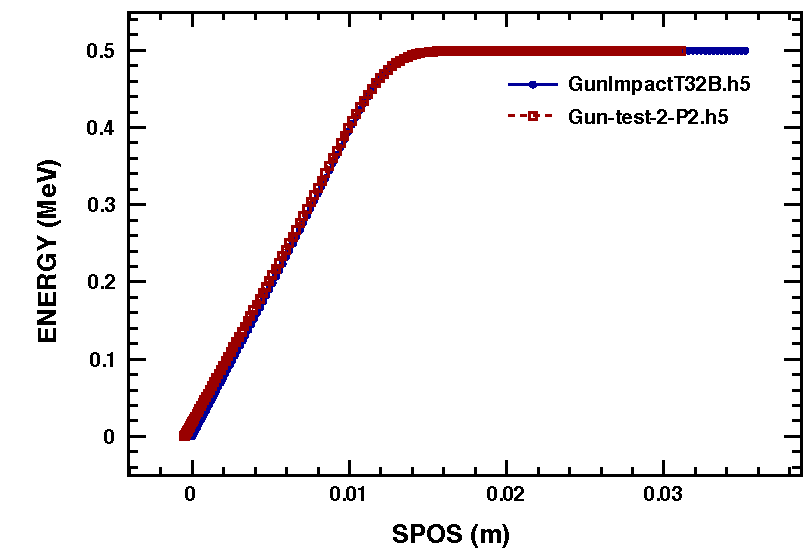
\includegraphics[width=0.60\linewidth,angle=90]{figures/Gun/GunCompEn}
   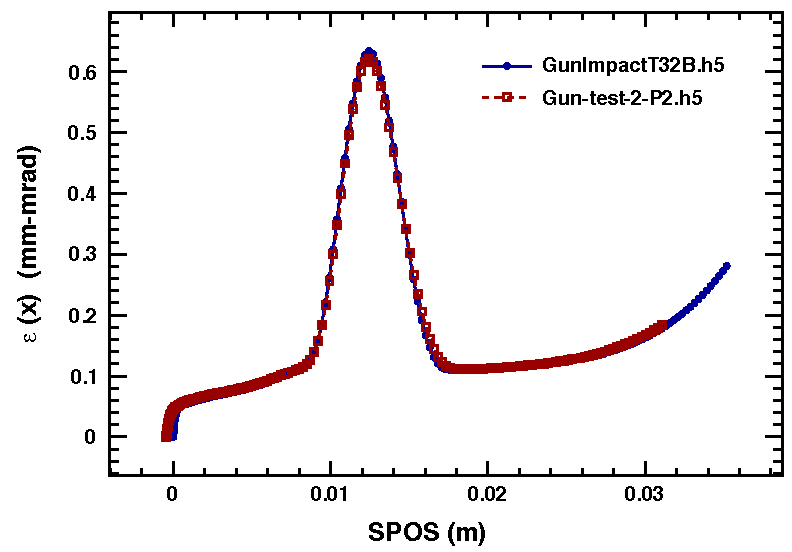
\includegraphics[width=0.60\linewidth,angle=90]{figures/Gun/GunCompEx}
   \caption{Comparison of energy and emittance in $x$ between \impactt and \opalt}   
   \label{fig:guncomp2}
 \end{center}
\end{figure}

\subsection{PSI XFEL 250 MeV Injector}
\label{sec:felinj}
\index{XFEL}
\index{INJECTOR}
\clearpage

\subsection{PSI XFEL 30 MeV Diagnostic Section}
\label{sec:feldiagsec1}
\index{XFEL}
\index{DIAGNOSTIC-1}
\begin{verbatim}
Option, ECHO=FALSE;
Option, TFS=FALSE;
Option, PSDUMPFREQ=10;

Title,string="OPAL Diagnostics test";

Edes=0.0307; //GeV
gamma=(Edes+EMASS)/EMASS;
beta=sqrt(1-(1/gamma^2));
gambet=gamma*beta;
P0 = gamma*beta*EMASS;
brho = (EMASS*1.0e9*gambet) / CLIGHT;
value,{gamma,brho,Edes,beta,gambet};

FINLB02_MSLAC40: Solenoid, L=0.001, KS=0.05, 
                                       FMAPFN="FINLB02-MSLAC.T7", ELEMEDGE=4.554;

FIND1_MQ10: Quadrupole, L=0.1, K1=2.788, ELEMEDGE=5.874;
FIND1_MQ20: Quadrupole, L=0.1, K1=-3.517, ELEMEDGE=6.074;


SCREEN: Monitor, L=0.01, ELEMEDGE=7.3867, OUTFN="Screen.h5";

FIND1:   Line = (FINLB02_MSLAC40, FIND1_MQ10, FIND1_MQ20, SCREEN);

Dist1:DISTRIBUTION, DISTRIBUTION=gauss,
                    sigmax=  1.0e-03, sigmapx=1.0e-4, corrx=0.5,
                    sigmay=  2.0e-03, sigmapy=1.0e-4, corry=-0.5,
                    sigmat=  3.0e-03, sigmapt=1.0e-4, corrt=0.0;

Fs2:FIELDSOLVER, FSTYPE=FFT, MX=32, MY=32, MT=64, 
                 PARFFTX=false, PARFFTY=false, PARFFTT=true,
                 BCFFTX=open, BCFFTY=open, BCFFTT=open,
                 BBOXINCR=1.0, GREENSF=INTEGRATED;

beam1: BEAM, PARTICLE=ELECTRON, pc=P0, NPART=1e5, 
               BFREQ=1498.953425154e6, BCURRENT=0.299598, CHARGE=-1;

Select, Line=FIND1;

track,line=FIND1, beam=beam1, MAXSTEPS=10000, DT=1.0e-12;
 run, method = "PARALLEL-T", beam=beam1, 
         fieldsolver=Fs2, distribution=Dist1;
endtrack;
Stop;
\end{verbatim}



\subsection{PSI  Injector II Cyclotron}
\label{sec:inj2}
\index{INJECTOR II}
\index{CYCLOTRON}
%%%%%%%%%%
Injector II is a separated sector cyclotron specially designed for preacceleration (inject: 870keV, extract: 72MeV )
of high intensity proton beam for Ring cyclotron. It has 4 sector magnets, two double-gap acceleration cavities 
(represented by 2 single-gap cavities here) and two single-gap flat-top cavities.  

Following is an input file of {\bfseries Single Particle Tracking mode} for PSI Injector II cyclotron.
{ \footnotesize 
\begin{verbatim}

// file name ''testinj2-1.in''

Option, TFS=FALSE;
Option, ECHO=FALSE;
Option, PSDUMPFREQ=100000;
Option, SPTDUMPFREQ=5;

Title,string="OPAL-CyclT test";

// define some physical parameters 
Edes=0.002;
gamma=(Edes+PMASS)/PMASS;
beta=sqrt(1-(1/gamma^2));
gambet=gamma*beta;
P0 = gamma*beta*PMASS;
brho = (PMASS*1.0e9*gambet) / CLIGHT;
value,{gamma,brho,Edes,beta,gambet};
phi01= 48.4812-15.0;
phi02=phi01+200.0;
phi03=phi01+1800.0;
phi04=phi01+2000.0;
phi05=(phi01+820.0)*3.0;
phi06=(phi01+2620.0)*3.0;

// define elements and beamline
inj2: Cyclotron, TYPE="Injector2", CYHARMON=10, PHIINIT=30.0, PRINIT=-0.0067,
      RINIT=392.5, SYMMETRY=1.0, RFFREQ=frequency, FMAPFN="../ZYKL9Z.NAR";

rf0: RFCavity, VOLT=0.25796, FMAPFN="../av1.dat", TYPE="SINGLEGAP", 
       FREQ=frequency, RMIN = 350.0, RMAX = 3350.0, ANGLE=35.0,
       PDIS = 0.0, GAPWIDTH = 0.0, PHI0=phi01; 

rf1: RFCavity, VOLT=0.25796, FMAPFN="../av1.dat", TYPE="SINGLEGAP", 
       FREQ=frequency, RMIN = 350.0, RMAX = 3350.0, ANGLE=55.0,
       PDIS = 0.0, GAPWIDTH = 0.0, PHI0=phi02; 

rf2: RFCavity, VOLT=0.25796, FMAPFN="../av1.dat", TYPE="SINGLEGAP", 
       FREQ=frequency, RMIN = 350.0, RMAX = 3350.0, ANGLE=215.0,  
       PDIS = 0.0, GAPWIDTH = 0.0, PHI0=phi03; 

rf3: RFCavity, VOLT=0.25796, FMAPFN="../av1.dat", TYPE="SINGLEGAP", 
       FREQ=frequency, RMIN = 350.0, RMAX = 3350.0, ANGLE=235.0,  
       PDIS = 0.0, GAPWIDTH = 0.0, PHI0=phi04; 

rf4: RFCavity, VOLT=0.06380, FMAPFN="../av3.dat", TYPE="SINGLEGAP", 
       FREQ=frequency3, RMIN = 830.0, RMAX = 3330.0, ANGLE=135.0,
       PDIS = 0.0, GAPWIDTH = 0.0, PHI0=phi05; 

rf5: RFCavity, VOLT=0.06380, FMAPFN="../av3.dat", TYPE="SINGLEGAP", 
       FREQ=frequency3, RMIN = 830.0, RMAX = 3330.0, ANGLE=315.0, 
       PDIS = 0.0, GAPWIDTH = 0.0, PHI0=phi06; 

l1:   Line = (inj2,rf0,rf1,rf2,rf3,rf4,rf5);


// define particles distribution, read from file
Dist1:DISTRIBUTION, DISTRIBUTION=fromfile,FNAME="PartDatabase.dat"; 

// define fieldsolver, useless for single particle track mode 
Fs1:FIELDSOLVER, FSTYPE=FFT, MX=64, MY=64, MT=64, 
		 PARFFTX=true, PARFFTY=true, PARFFTT=false,
		 BCFFTX=open, BCFFTY=open, BCFFTT=open;
		 
// define beam parameters
beam1: BEAM, PARTICLE=PROTON, pc=P0, SPACECHARGE=false, 
	      NPART=1, BCURRENT=0.0;

// select beamline
Select, Line=l1;

// start tracking
track,line=l1, beam=beam1, MAXSTEPS=100*19750, DT=0.01e-9;
 run, file = "track_output", turns = 1, method = "CYCLOTRON-T",
      beam=beam1, fieldsolver=Fs1, distribution=Dist1;
endtrack;
Stop;

\end{verbatim}
}
To run opal on a single node, just use this command:
{ \footnotesize 
\begin{verbatim}
 opal testinj2-1.in --commlib mpi --info 0 | tee testinj2-1.out
\end{verbatim}
}
Here shows some pictures using the resulting data from single particle tracking using \opalcycl.

Figure \ref{fig:reftrack} shows The accelerating orbit of reference particle. After 106 turns, the energy increases from 870KeV at
the Injection point to 72.16MeV at the deflection point . 
\begin{figure}[ht]
 \begin{center} 
   \includegraphics[width=0.8\linewidth,angle=0]{figures/cyclotron/AEO_Injector2.png}
   \caption{Reference particle tracking in Injector II}
   \label{fig:reftrack}
 \end{center}
\end{figure}

From theoretic view, there should be an eigen ellipse for any given energy in stable area of a fixed accelerator structure. Only when the initial phase space
shape matches its eigen ellipse, the oscillation of beam envelop amplitude will get minimal and the transmission efficiency get maximal.
We can calculate the eigen ellipse by single particle tracking using betatron oscillation property of off-centered particle as following: track 
an off-centered particle and record its coordinates and momenta at the same azimuthal position for each revolution.    
Figure \ref{fig:eigen} shows the eigen ellipse at symmetric line of sector magnet for energy of 2 MeV in Injector II.
\begin{figure}[ht]
 \begin{center} 
   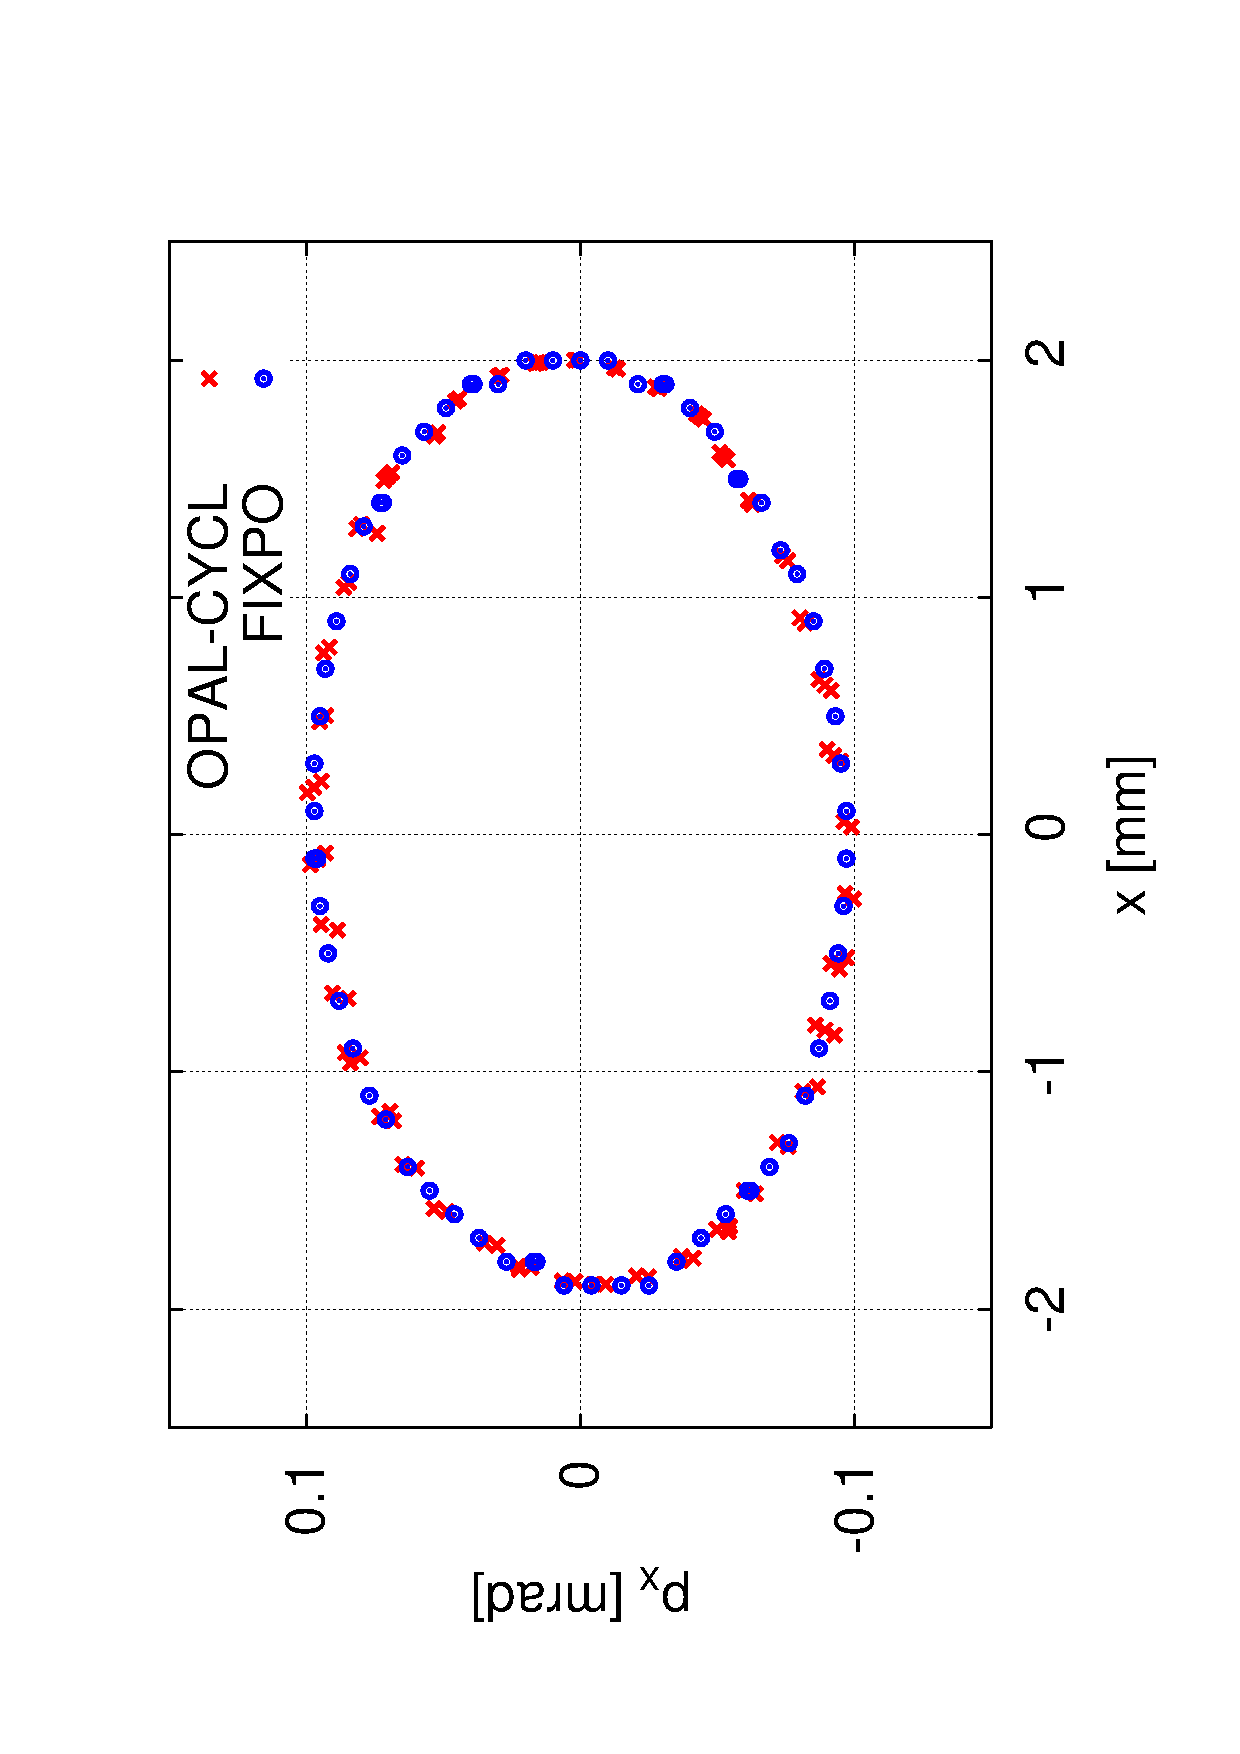
\includegraphics[width=0.45\linewidth,angle=0]{figures/cyclotron/RadialEigen_Inj2}
   \includegraphics[width=0.45\linewidth,angle=0]{figures/cyclotron/VertEigen_Inj2}
   \caption{radial and vertical eigenellipse at 2MeV}   
   \label{fig:eigen}
 \end{center}
\end{figure}
 
Figure \ref{fig:tuning} shows the tune diagram of Injector II obtained by \opalcycl and FIXPO.
The trivial discrepancy should come from the methods they used.
In FIXPO, the tune values are obtained according to the crossing points of the initially displaced particle. Meanwhile, in \opalcycl, the Fourier 
analysis method is used to manipulate orbit difference between the reference particle and an initially displaced particle.
The frequency point with the biggest amplitude is the betatron tune value at the given energy.
\begin{figure}[ht]
  \begin{center} 
    \includegraphics[width=0.8\linewidth,angle=0]{figures/cyclotron/nurnuz}
    \caption{Tune diagram of Injector II}
    \label{fig:tuning}
  \end{center}
\end{figure}

%%%%%%%%%%%%%%
Following is the input file for single bunch tracking with space charge effects in Injector II.
%%%%%%%%%%%%%% 
{ \footnotesize
\begin{verbatim}
 
// file name ''testinj2-2.in''
// Define Option parameters 
Option, ECHO=FALSE;
Option, PSDUMPFREQ=10;
Option, SPTDUMPFREQ=5;
Option, REPARTFREQ=10;

// Define title
Title,string="OPAL-CyclT-SC test";

// define some physical parameters 
Edes=0.000870;
gamma=(Edes+PMASS)/PMASS;
beta=sqrt(1-(1/gamma^2));
gambet=gamma*beta;
P0 = gamma*beta*PMASS;
brho = (PMASS*1.0e9*gambet) / CLIGHT;

phi01= 48.4812-15.0;
phi02=phi01+200.0;
phi03=phi01+1800.0;
phi04=phi01+2000.0;
phi05=(phi01+820.0)*3.0;
phi06=(phi01+2620.0)*3.0;

frequency=50.6370;
frequency3=3.0*frequency;

// define elements and beamline
inj2: Cyclotron, TYPE="Injector2", CYHARMON=10, PHIINIT=30.0,PRINIT=-0.0067,
RINIT=392.5, SYMMETRY=1.0, RFFREQ=50.6370,FMAPFN="../../ZYKL9Z.NAR";

rf0: RFCavity, VOLT=0.25796, FMAPFN="../../Cav1.dat", TYPE="SINGLEGAP",
FREQ=50.637, RMIN = 350.0, RMAX = 3350.0, ANGLE=35.0,   PDIS = 0.0,
GAPWIDTH = 0.0, PHI0=phi01;
rf1: RFCavity, VOLT=0.25796, FMAPFN="../../Cav1.dat", TYPE="SINGLEGAP",
FREQ=50.637, RMIN = 350.0, RMAX = 3350.0, ANGLE=55.0,   PDIS = 0.0,
GAPWIDTH = 0.0, PHI0=phi02;
rf2: RFCavity, VOLT=0.25796, FMAPFN="../../Cav1.dat", TYPE="SINGLEGAP",
FREQ=50.637, RMIN = 350.0, RMAX = 3350.0, ANGLE=215.0,  PDIS = 0.0,
GAPWIDTH = 0.0, PHI0=phi03;
rf3: RFCavity, VOLT=0.25796, FMAPFN="../../Cav1.dat", TYPE="SINGLEGAP",
FREQ=50.637, RMIN = 350.0, RMAX = 3350.0, ANGLE=235.0,  PDIS = 0.0,
GAPWIDTH = 0.0, PHI0=phi04;
rf4: RFCavity, VOLT=0.06380, FMAPFN="../../Cav3.dat", TYPE="SINGLEGAP",
FREQ=151.911, RMIN = 830.0, RMAX = 3330.0, ANGLE=135.0, PDIS = 0.0,
GAPWIDTH = 0.0, PHI0=phi05;
rf5: RFCavity, VOLT=0.06380, FMAPFN="../../Cav3.dat", TYPE="SINGLEGAP",
FREQ=151.911, RMIN = 830.0, RMAX = 3330.0, ANGLE=315.0, PDIS = 0.0,
GAPWIDTH = 0.0, PHI0=phi06;

l1:   Line = (inj2,rf0,rf1,rf2,rf3,rf4,rf5);

// define particles distribution, generate Gaussion type
Dist1:DISTRIBUTION, DISTRIBUTION=gauss,
sigmax=  2.0e-03, sigmapx=1.0e-7, corrx=0.0,
sigmay=  2.0e-03, sigmapy=1.0e-7, corry=0.0,
sigmat=  2.0e-03, sigmapt=1.8e-4, corrt=0.0;

// define parallel FFT fieldsolver, parallel in x y direction
Fs1:FIELDSOLVER, FSTYPE=FFT, MX=32, MY=32, MT=32, 
		 PARFFTX=true, PARFFTY=true, PARFFTT=false,
		 BCFFTX=open, BCFFTY=open, BCFFTT=open,BBOXINCR=5;

// define beam parameters
beam1: BEAM, PARTICLE=PROTON, pc=P0, SPACECHARGE=true,
       NPART=1e5, BCURRENT=3.0E-3, CHARGE=1.0, BFREQ= frequency;

// select beamline
Select, Line=l1;

// start tracking
track,line=l1, beam=beam1, MAXSTEPS=80*2000, DT=0.1e-9;
 run, file = "track_output", turns = 1, method = "CYCLOTRON-T", 
      beam=beam1, fieldsolver=Fs1, distribution=Dist1;
endtrack;
Stop;
\end{verbatim}
}
To run opal on single node, just use this command:
{ \footnotesize 
\begin{verbatim}
 # opal testinj2-2.in --commlib mpi --info 0 | tee testinj2-2.out
\end{verbatim}
}
To run opal on N nodes in parallel environment interactively, use this command instead:
{ \footnotesize 
\begin{verbatim}
 # mpirun -np N opal testinj2-2.in  --commlib mpi 
   --info 0 | tee testinj2-2.out
\end{verbatim}
 }
If restart a job from the last step NSTEP of an existing $.h5$ file, add a new argument like this: 
{ \footnotesize 
\begin{verbatim}
 # mpirun -np N opal testinj2-2.in --restart NSTEP 
   --commlib mpi --info 0 | tee testinj2-2.out
\end{verbatim}
}
Figure \ref{fig:cyclParameters} and \ref{fig:cyclphasespace} are from preliminary simulation results.
They are generated by H5partROOT code.   
\begin{figure}[ht]
  \begin{center} 
    \includegraphics[width=0.45\linewidth]{figures/cyclotron/Inj2-ENERGY-TIME.png}
    \includegraphics[width=0.45\linewidth]{figures/cyclotron/Inj2-B-ref-z-TrackStep.png}
    \caption{Energy Vs. time (left) and external B field Vs. trackstep (Right, only show for about 2 turns)}
    \label{fig:cyclParameters}
  \end{center}
\end{figure}

\begin{figure}[ht]
  \begin{center} 

    \includegraphics[width=0.3\linewidth]{figures/cyclotron/Inj2-z-pz-step-870KeV.png}
    \includegraphics[width=0.3\linewidth]{figures/cyclotron/Inj2-z-pz-step-15MeV.png}
    \includegraphics[width=0.3\linewidth]{figures/cyclotron/Inj2-z-pz-step-30MeV.png}
    \caption{Vertical phase at different energy from left to right: 0.87,15 and 35( MeV}
    \label{fig:cyclphasespace}
  \end{center}
\end{figure}

%%%%%%%%%%%%%%
\subsection{PSI  Ring Cyclotron}
\label{sec:Ring}
\index{RING}
\index{CYCLOTRON}
From the view of numerical simulation, the difference between Injector II and Ring cyclotron comes from two aspects:
\begin{description}
\item[B Field] The structure of Ring is totally symmetric, the field on median plain is periodic 
along azimuthal direction, \opalcycl take this advantage to only store 1/8 field data to save memory.

\item[RF Cavity] In the Ring, all the cavities are typically single gap with some parallel displacement from its
radial position.\opalcycl have an argument \texttt{PDIS} to manipulate this issue.  
\end{description}
\begin{figure}[ht]
  \begin{center} 
    \includegraphics[width=0.8\linewidth,angle=0]{figures/cyclotron/AEO_Ring.png}
    \caption{Reference particle tracking in 590MeV Ring}
    \label{fig:reference orbit}
  \end{center}
\end{figure}

\begin{figure}[ht]
  \begin{center} 
    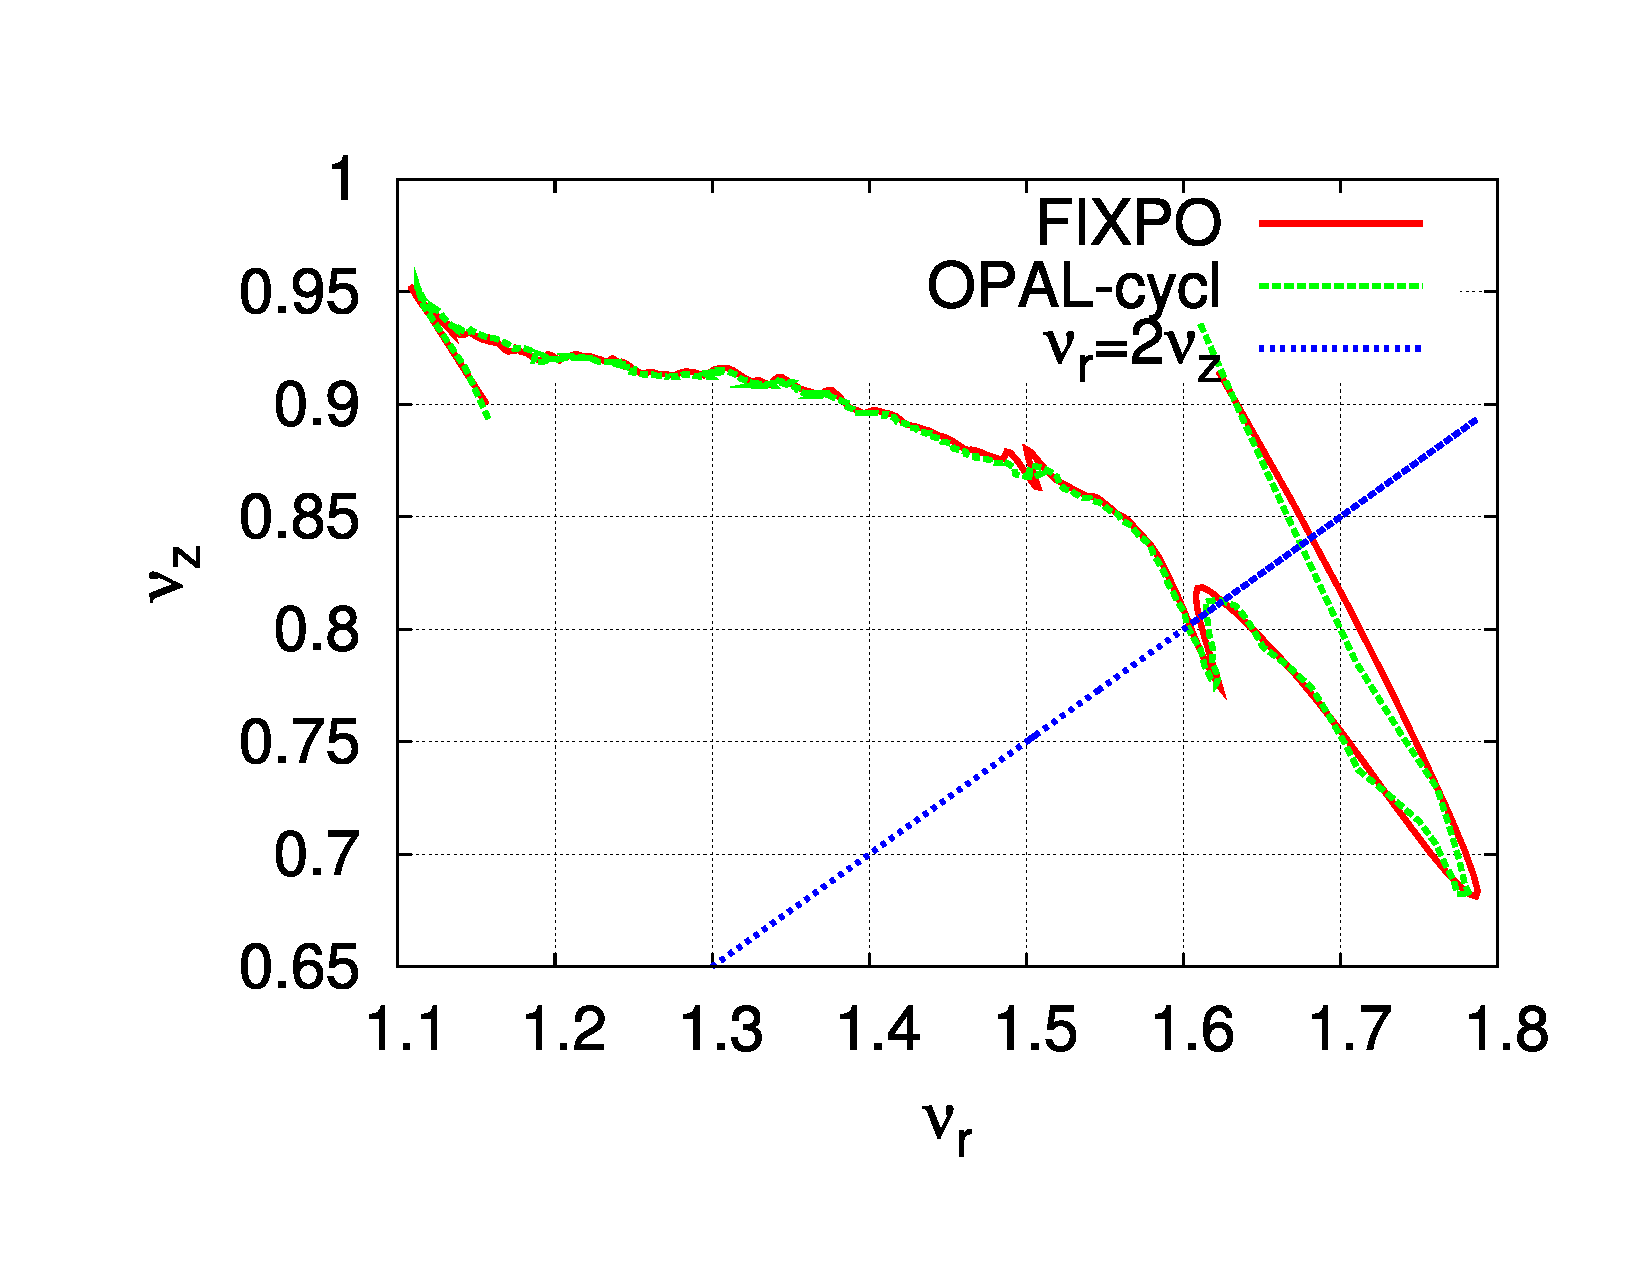
\includegraphics[width=0.8\linewidth,angle=0]{figures/cyclotron/nurnuz_Ring}
    \caption{Tune diagram of 590MeV Ring}
    \label{fig:TuningRing}
  \end{center}
\end{figure}


Figure \ref{fig:reference orbit} and \ref{fig:TuningRing} are from perliminary resutls.
Limited by size of the user guide, we don't plan to show too much details as in Injector II.

\clearpage
\subsection{CERN SPS Lattice}
\label{sec:sps}
\index{SPS}
The CERN SPS lattice may be represented using the following beam elements:
\begin{verbatim}
QF:QUADRUPOLE,...; // focusing quadrupole
QD:QUADRUPOLE,...; // defocusing quadrupole
B1:RBEND,...;      // bending magnet of type 1
B2:RBEND,...;      // bending magnet of type 2
DS:DRIFT,...;      // short drift space
DM:DRIFT,...;      // drift space replacing two bends
DL:DRIFT,...;      // long drift space
\end{verbatim}
The SPS machine is represented by the lines
\begin{verbatim}
SPS:   LINE=(6*SUPER);
SUPER: LINE=(7*P44,INSERT,7*P44);
INSERT:LINE=(P24,2*P00,P42);
P00:   LINE=(QF,DL,QD,DL);
P24:   LINE=(QF,DM,2*B2,DS,PD);
P42:   LINE=(PF,QD,2*B2,DM,DS);
P44:   LINE=(PF,PD);
PD:    LINE=(QD,2*B2,2*B1,DS);
PF:    LINE=(QF,2*B1,2*B2,DS);
\end{verbatim}
In order not to overload the example,
small gaps between magnetic elements have been omitted.

\subsection{LEP Lattice}
\label{sec:lep}
\index{LEP}
A preliminary description of LEP has been given in the
\bibref{LEP pink book}{LEP}.
Translation of those element sequences to the \opal input format gives:
\begin{verbatim}
LEP: LINE=(4*SUP);
SUP: LINE=(OCT,-OCT);
OCT: LINE=(LOBS,RFS,DISS,ARC,DISL,RFL,LOBL);
LOBS:LINE=(L1,QS1,L2,QS2,L3,QS3,L4,QS4);
RFS: LINE=(L5,QS5,L5,QS6,L5,2*(QS7,L5,QS8,L5));
DISS:LINE=(QS11,L25,BW,L22,QS12,L25,B4,L22,QS13,L25,B4,
           L22,QS14,L25,B4,L31,QS15,L25,B4,L32,SF,L23,QS16);
ARC: LINE=(L21,B6,L22,SD,L23,QD,
           7*(CELL(SF1,SD1),CELL(SF,SD)),CELL(SF1,SD1),
           L24,B6,L41,QF,L21,B6,L22,SD4,L23,QD,
           7*(CELL(SF4,SD3),CELL(SF3,SD4)),CELL(SF4,SD3),
           L24,B6,L22,SF3,L23);
DISL:LINE=(QL16,L34,B4,L22,QL15,L33,B4,L22,QL14,L25,B4,
           L22,QL13,L25,B4,L22,QL12,L25,BW,L22,QL11);
RFL: LINE=(2*(L5,QL8,L5,QL7),L5,QL6,L5,QL5,L5);
LOBL:LINE=(QL4,L14,QL3,L13,QL2,L12,QL1,L11);
BW:  LINE=(W,L26,W);
B4:  LINE=(B,L26,B);
B6:  LINE=(B,L26,B,L26,B);
CELL(SF,SD):LINE=(L24,B6,L22,SF,L23,QF,L21,B6,L22,SD,L23,QD);
\end{verbatim}
Here the element definitions have been left out to save space.
                 % ch 9
\ifdefined \buildingFullOPALManual \else


%\ifx \@buildingFullOPALManual \@empty
%\else

%\documentclass[12pt,a4paper]{report}
\documentclass[a4paper]{book}

%% does not work in Latex2Html mode
%\usepackage{hyperref}

\usepackage[T1]{fontenc}
\usepackage{url}
\usepackage{html}
\usepackage{epic}
\usepackage{eepic}
\usepackage{makeidx}
\usepackage{array}
\usepackage{times}
\usepackage{amsmath}
\usepackage{amsxtra}
\usepackage{bm}
\usepackage[thin,thinp,thinc]{esdiff}
\usepackage{etoolbox}
\usepackage{graphicx}
\usepackage{dingbat}
\usepackage{color}
\usepackage{subfig}
\usepackage{boxedminipage}
\usepackage{alltt}
\usepackage{nicefrac}
\usepackage{calc}
%\usepackage{pdfdraftcopy}             % Draft
\usepackage{tikz}
\usetikzlibrary{
  er,3d,calc,fadings,trees,positioning,arrows,chains,decorations.pathreplacing,
  decorations.pathmorphing,shapes,shapes.symbols,shapes.arrows,matrix,through,decorations.text
}

\tikzset{
  >=stealth',
  punktchain/.style={rectangle,rounded corners, draw=black, very thick,text width=10em,
                     minimum height=3em, text centered, on chain},
  line/.style={draw, thick, <-},
  element/.style={tape,top color=white,bottom color=blue!50!black!60!,minimum width=8em,
                  draw=blue!40!black!90, very thick,text width=10em, minimum height=3.5em,
                  text centered, on chain},
  every join/.style={->, thick,shorten >=1pt},
  tuborg/.style={decorate},
  tubnode/.style={midway, right=2pt}
}

\tikzstyle{material}=[draw, fill=blue!20, text width=16.0em, text centered, minimum height=1.5em]
\tikzstyle{diagramstep} = [material, text width=20em, minimum width=10em, minimum height=3em, rounded corners]
\tikzstyle{line} = [draw, thick, color=black!50, -latex']

\usepackage{booktabs}
\usepackage{xspace}
\usepackage{xstring}

\usepackage{fancyvrb}
\usepackage{rotating}
\usepackage{float}

\usepackage{tabularx}
\usepackage{longtable}
\setcounter{LTchunksize}{3}

\usepackage[section]{placeins}
\usepackage{MnSymbol}
\usepackage{microtype}
\usepackage{setspace}
\usepackage{dcolumn}

\usepackage[vmargin={3.0cm,3.0cm},
            hmargin={2.0cm,3.0cm}]{geometry}

\usepackage{upgreek}
\usepackage[binary-units=true]{siunitx}
\sisetup{exponent-product = \cdot,math-ohm=\Upomega,text-ohm=\ensuremath{\Upomega}}
\DeclareSIUnit{\clight}{c}
\DeclareSIUnit\gauss{Ga}

\usepackage{engord}
\usepackage{wasysym}
\DeclareSIUnit[number-unit-product = \,]{\permill}{\permil}

\usepackage{hyperref}
\hypersetup{
    pdftitle          = The OPAL Framework,
    pdfauthor         = {Andreas Adelmann, Achim Gsell, Valeria Rizzoglio, Christof Metzger-Kraus,
                         Yves Ineichen, Xiaoying Pang, Steve Russell, Chuan Wang, Jianjun Yang,
                         Suzanne Sheehy, Chris Rogers, Daniel Winklehner},
    pdfsubject        = User's Reference Manual,
    pdffitwindow      = true,               % page fit to window when opened
    pdfnewwindow      = true,               % links in new window
    colorlinks        = true,               % false: boxed links; true: colored links
    linkcolor         = black!80!green,     % color of internal links
    citecolor         = black!20!red,       % color of links to bibliography
    urlcolor          = blue,               % color of external links
    breaklinks        = true,
    bookmarksnumbered = true,
    plainpages        = false
}

\usepackage{ifthen}

\newif \iflinuxwindows
\linuxwindowstrue   % set this to true when building the manual on Linux or Windows
\iflinuxwindows
\usepackage{epstopdf}
\fi

\usepackage[backend=biber,
            style=phys,
            biblabel=brackets,
            maxnames=3,
            doi=true,
            isbn=true,
            url=true]{biblatex}
%---- macros ----

\renewcommand{\topfraction}{1.0}
\renewcommand{\bottomfraction}{1.0}
\renewcommand{\textfraction}{0.0}
\renewcommand{\arraystretch}{2.0}
\newenvironment{tex2html_nowrap}{}{}


\newcommand{\Newline}{\hfil \\}


\newsavebox{\ExampleBox}
\newenvironment{example}
 {\VerbatimEnvironment
  \begin{flushleft}
  \begin{lrbox}{\ExampleBox}
    \begin{minipage}{\linewidth}
  \begin{Verbatim}[frame=lines,xleftmargin=0cm,fontsize=\footnotesize,samepage=true]}
 {\end{Verbatim}
  \end{minipage}
  \end{lrbox}
  \mbox{\usebox{\ExampleBox}}
  \end{flushleft}
 }

\newenvironment{longexample}
{\Verbatim[frame=lines,xleftmargin=0mm,fontsize=\footnotesize]}
{\endVerbatim}

%\examplefromfile{filename} reads in a text file and displays it in the document.
\newcommand{\examplefromfile}[1]{
\VerbatimInput[frame=lines,xleftmargin=0mm,fontsize=\footnotesize,label=\texttt{#1}]{#1}}

%for upright d of differentials
\makeatletter
\newcount\my@repeat@count

\newcommand{\myrepeat}[2]{%
  \begingroup
  \my@repeat@count=\z@
  \@whilenum\my@repeat@count<#1\do{#2\advance\my@repeat@count\@ne}%
  \endgroup
}

\newcommand{\differential}[1]{\ifstrempty{#1}{\ES@dop\ES@difint}{\ES@dop^{#1}\ES@difint}}
\newcommand{\pdifferential}[1]{\ifstrempty{#1}{{\partial\,}}{{\partial^{#1}\,}}}

\makeatother

\newcommand{\der}[3][]{\frac{\differential{#1}#2}{\differential{}\ifstrempty{#1}{#3}{#3^#1}}}
\newcommand{\parder}[3][]{\frac{\pdifferential{#1}#2}{\pdifferential{}\ifstrempty{#1}{#3}{#3^#1}}}
\newcommand{\niceder}[3][]{\nicefrac{\differential{#1}#2}{\differential{}\ifstrempty{#1}{#3}{#3^#1}}}
\newcommand{\uglyder}[3][]{{\differential{#1}#2}/{\differential{}\ifstrempty{#1}{#3}{#3^#1}}}
\newcommand{\uglyparder}[3][]{{\pdifferential{#1}#2}/{\pdifferential{}\ifstrempty{#1}{#3}{#3^#1}}}
\newcommand{\dd}[1][]{\; \differential{#1}}
\newcommand{\primed}{^{\prime}}
\newcommand{\dprimed}{^{\prime\prime}}
\newcommand{\nprimed}[1]{^{\myrepeat{#1}{\prime}}}

%Editing Macros
\newcommand{\TODO}[1]{{\color{red}\ifthenelse{\boolean{ShowDebug}}{[TODO: #1]}{}}}



%text in gray box
\newsavebox{\fmbox}
\definecolor{lightgray}{gray}{0.95}
\newenvironment{fmpage}
   {\vspace{-1.0cm}\begin{lrbox}{\fmbox}\begin{minipage}[t]{13.5cm}\vspace{0.1cm}}
   {\vspace{-0.4cm}\end{minipage}\end{lrbox}\begin{center}\fcolorbox{black}{lightgray}{\usebox{\fmbox}}\end{center}}


% Definition new signes
\newcommand{\R}{{\mathbb R}} % real numbers
\newcommand{\Q}{{\mathbb Q}} % rational numbers
\newcommand{\Z}{{\mathbb Z}} % integer numbers
\newcommand{\N}{{\mathbb N}} % natural numbers

\newcommand{\mad}{\textsc{mad}\xspace}
\newcommand{\madnine}{\textsc{mad9}\xspace}
\newcommand{\madninep}{\textsc{mad9p}\xspace}
\newcommand{\madeight}{\textsc{mad8}\xspace}
\newcommand{\classic}{\textsc{classic}\xspace}

\makeatletter
\newcommand{\opal@impl}{\textsc{Opal}}
\newcommand{\opalt@impl}{\textsc{Opal-t}}
\newcommand{\opalcycl@impl}{\textsc{Opal-cycl}}
\newcommand{\opalmap@impl}{\textsc{Opal-map}}
\newcommand{\opalenv@impl}{\textsc{Opal-e}}

\newcommand{\opal}{\opal@impl\xspace}
\newcommand{\opalt}{\opalt@impl\xspace}
\newcommand{\opalcycl}{\opalcycl@impl\xspace}
\newcommand{\opalmap}{\opalmap@impl\xspace}
\newcommand{\opalenv}{\opalenv@impl\xspace}

\newcommand{\noopalt}{\leftthumbsdown \opalt@impl\xspace}
\newcommand{\noopalcycl}{\leftthumbsdown \opalcycl@impl\xspace}
\newcommand{\noopalmap}{\leftthumbsdown \opalmap@impl\xspace}
\newcommand{\noopalenv}{\leftthumbsdown \opalenv@impl\xspace}
\makeatother

\newcommand{\impactt}{\textsc{Impact-t}\xspace}
\newcommand{\partroot}{\textsc{H5root}}


\newcommand{\latermore}{More details will be given in Version 1.6.0}


\newcommand{\lieop}[1]{{:}{#1}{:}}

\newcommand{\rms}[1]{\overset{\sim}{#1}}

\newcommand{\sprod}{\cdot}
\newcommand{\vprod}{\times}
\newcommand{\matr}[1]{\mathcal{#1}}
\renewcommand{\vec}[1]{{\bm{#1}}}
\newcommand{\transpose}[1]{#1^\intercal}
\renewcommand{\epsilon}{\varepsilon}

\newcommand{\keyword}[2][]{\ifstrempty{#1}{\texttt{\expandafter\MakeUppercase\expandafter{#2}}}{\hyperref[#1]{\texttt{\expandafter\MakeUppercase\expandafter{#2}}}}}
\newcommand{\tabline}[3][]{\keyword[#1]{#2}& #3 \\}
\newcommand{\tabheadcell}[1]{{\bfseries #1}}

\newcommand*\kdescriptionlabel[1]{\hspace\labelsep
                                \normalfont\keyword{#1}\index{#1}}
\makeatletter
\newenvironment{kdescription}
               {\list{}{\labelwidth\z@ \itemindent-\leftmargin
                        \let\makelabel\kdescriptionlabel}}
               {\endlist}
\makeatother

\ExplSyntaxOn
\NewDocumentCommand{\tabhead}{ m }
 {
  \seq_set_split:Nnn \l_tmpa_seq { & } { #1 }
  \bfseries \seq_use:Nn \l_tmpa_seq { & \bfseries } \\
 }

\NewDocumentCommand \multrefImpl { O{ } m m m } {
  \ifnumgreater{\clist_count:n {#4}}{1}{
    \seq_set_from_clist:Nn \l_tmpa_seq { #4 }

    \seq_set_map:NNn \l_tmpb_seq \l_tmpa_seq { \exp_not:n { \ref{#3:##1} } }
    \ifstrempty{#1}{#2s}{#1}~\seq_use:Nnnn \l_tmpb_seq {\ and\ } {,\ } {,\ and\ }
  }{
    #2~\ref{#3:#4}
  }
}

\NewDocumentCommand \multeqnrefImpl { m } {
  \ifnumgreater{\clist_count:n {#1}}{1}{
    \seq_set_from_clist:Nn \l_tmpa_seq { #1 }

    \seq_set_map:NNn \l_tmpb_seq \l_tmpa_seq { \exp_not:n { \eqref{eq:##1} } }
    Equations~\seq_use:Nnnn \l_tmpb_seq {\ and\ } {,\ } {,\ and\ }
  }{
    Equation~\eqref{eq:#1}
  }
}
\ExplSyntaxOff


%Abbreviations for Equations, Figures, and Tables
%\newcommand{\Equation}[1]{Equation~\eqref{#1}}

\newcommand{\bibref}[2]{#1 \cite{bib:#2}}
\newcommand{\figref}[1]{\multrefImpl{Figure}{fig}{#1}}
\newcommand{\chpref}[1]{\multrefImpl{Chapter}{chp}{#1}}
\newcommand{\appref}[1]{\multrefImpl[Appendices]{Appendix}{chp}{#1}}
\newcommand{\secref}[1]{\multrefImpl{Section}{sec}{#1}}
\newcommand{\ssecref}[1]{\multrefImpl{Section}{ssec}{#1}}
\newcommand{\tabref}[1]{\multrefImpl{Table}{tab}{#1}}
\newcommand{\eqnref}[1]{\multeqnrefImpl{#1}}

\newcommand{\seefig}[1]{(see~\figref{#1})}
\newcommand{\seechp}[1]{(see~\chpref{#1})}
\newcommand{\seesec}[1]{(see~\secref{#1})}
\newcommand{\seessec}[1]{(see~\ssecref{#1})}
\newcommand{\seetab}[1]{(see~\tabref{#1})}
\newcommand{\seeeqn}[1]{(see~\eqnref{#1})}

\newcommand{\filename}[1]{\emph{#1}}


% Define distances for bordering
\newcommand{\blockdist}{1.3}
\newcommand{\edgedist}{1.5}
\newcommand{\diagramstep}[2]{node (p#1) [diagramstep] {#2}}


% place chapter title page on odd pages
\let\stdchapter\chapter
\makeatletter
\renewcommand*{\chapter}{\if@openright\cleardoublepage\else\clearpage\fi\stdchapter}

\makeatother

\IfFileExists{./version.tex}{%
  \input{version}%
}%
{%
  \input{noversion}%
}
\newboolean{ShowMap}
\setboolean{ShowMap}{false}

\newboolean{ShowEnv}
\setboolean{ShowEnv}{false}

\newboolean{ShowDebug}
\setboolean{ShowDebug}{false}

%----Control Structures
\newboolean{FullOPALManual}
\setboolean{FullOPALManual}{false}


\makeindex


\bibliography{bibliography}
\begin{document}

\fi

\chapter{Beam Command}
\label{chp:beam}
\index{BEAM}
All \opal commands working on a beam require the setting of various
quantities related to this beam.
These are entered by a \keyword{BEAM} command:
\begin{example}
label:BEAM, PARTICLE=name, MASS=real, CHARGE=real,
      ENERGY=real, PC=real, GAMMA=real, BCURRENT=real,
       NPART=real, BUNCHED=logical, BFREQ=real;
\end{example}
The \texttt{label} is optional, it defaults to \keyword{UNNAMED\_BEAM}.
\index{UNNAMED\_BEAM}. The particle mass and charge are defined by:
\begin{kdescription}
\item[PARTICLE]
  The name of particles in the machine.
\end{kdescription}

\opal knows the mass and the charge for the following particles:
\begin{kdescription}
  \item[POSITRON]
    The particles are positrons (\texttt{MASS}=$m_e$,
    \texttt{CHARGE}=1),

  \item[ELECTRON]
    The particles are electrons (\texttt{MASS}=$m_e$,
    \texttt{CHARGE}=-1),

  \item[PROTON]
    The particles are protons (default, \texttt{MASS}=$m_p$,
    \texttt{CHARGE}=1),

  \item[ANTIPROTON]
    The particles are anti-protons (\texttt{MASS}=$m_p$,
    \texttt{CHARGE}=-1).

  \item[HMINUS]
    The particles are h- protons (\texttt{MASS}=$m\_{h^{-}}$,
    \texttt{CHARGE}=-1).

  \item[CARBON]
    The particles are carbons (\texttt{MASS}=$m_c$,
    \texttt{CHARGE}=12).

  \item[URANIUM]
    The particles are of type uranium (\texttt{MASS}=$m_u$,
    \texttt{CHARGE}=35).

  \item[MUON]
    The particles are of type muon (\texttt{MASS}=$m_\mu$,
    \texttt{CHARGE}=-1).

  \item[DEUTERON]
    The particles are of type deuteron (\texttt{MASS}=$m_d$,
    \texttt{CHARGE}=1).

  \item[XENON]
    The particles are of type xenon (\texttt{MASS}=$m_{xe}$,
    \texttt{CHARGE}=20).
\end{kdescription}

For other particle names one may enter:
\begin{kdescription}
\item[MASS]
  \index{Particle!Mass}\index{Mass}
  The particle mass in GeV.
\item[CHARGE]
  \index{Particle!Charge}\index{Charge}
  The particle charge expressed in elementary charges.
\end{kdescription}

The other attributes are:

\begin{kdescription}
\item[BFREQ]
  The bunch frequency in MHz.
\item[BCURRENT]
The bunch current in A.
$\text{\keyword{BCURRENT}} = Q \times \text{\keyword{BFREQ}}$ with $Q$ the total charge.
\item[NPART]
The number of macro particles for the simulations
\end{kdescription}

%----------- Footer control ------------------
\ifthenelse{\boolean{FullOPALManual}}
{
  %do nothing
}
% else (for individual document creation)
{
\appendix
\printbibliography
\end{document}
}
%---------------------------------------------               % ch 10
\chapter{Distribution Command}
\label{sec:distribution}
\index{distr|(}
Particle distributions can be read in or generated by specifying rms beam quantities.
The allowed parameters are described in Table \ref{tab:distrparam}.

Particle distributions are generated separately in all three phase space planes.
There are no explicit correlations between planes e.g. between longitudinal and transverse.
Besides an efficient parallel Gaussian distribution generator based on a parallelized 
``Method of Rejection'',
a more general algorithm for generating
distributions is available \cite{JohoDist}. The shape of the binomial distribution is governed by
one parameter $m$. By varying this single parameter one obtains the most commonly 
used distributions for our
type of simulations as, listed in Table \ref{tab:binomdist}.

If NBIN is larger than one the distribution is binned in energy and for each bin a separate field solve is
performed when using the electrostatic solvers.
 
\begin{table}[h!]
\begin{flushleft} \footnotesize
 \begin{tabular}{|l|l|l|l|}
\hline
\bf m & \bf Distribution & \bf Density & \bf Profile \\
\hline
0.0 & Hollow shell  & $\frac{1}{\pi}\delta(1-r^2)$ &$\frac{1}{\pi}(1-r^2)^{-0.5}$\\
\hline
0.5 & Flat profile  & $\frac{1}{2\pi}(1-r^2)^{-0.5}$ & $\frac{1}{2}$\\
\hline
1.0 & Uniform  & $\frac{1}{\pi}$ & $\frac{2}{\pi}(1-x^2)^{0.5}$\\
\hline
1.5 & Elliptical  & $\frac{3}{2\pi}(1-r^2)^{0.5}$ & $\frac{1}{4}(1-x^2)$ \\
\hline
2.0 & Parabolic  & $\frac{2}{\pi}(1-r^2)$ & $\frac{3}{8\pi}(1-x^2)^{1.5}$ \\
\hline
$\rightarrow \infty$ & Gaussian  & $\frac{1}{2\pi\sigma_x\sigma_y}exp(-\frac{x^2}{2\sigma_x^2} -\frac{y^2}{2\sigma_y^2})$ & 
                       $\frac{1}{\sqrt{2\pi}*\sigma_x}exp(-\frac{x^2}{2\sigma_x^2}) $ \\
\hline
\end{tabular}
\end{flushleft} 
\caption{\label{tab:binomdist}{Different distributions specified by a single parameter $m$}}
\end{table}
There are also special distribution commands.
\begin{enumerate}
\item {\it GUNGAUSS} will create a distribution that is uniform in $x$ and $y$ (with the
radius in each plane given by SIGMAX and SIGMAX) and with a Gaussian distribution longitudinally (given by SIGMAT).
This distribution is cold in the transverse direction and has a uniform temperature given by the initial kinetic energy in
eV specified by the PT and the SIGMAPT variables.
\item {\it GUNGAUSS3D} is identical to {\it GUNGAUSS} except that it generates a distribution that is Gaussian in the
transverse planes as well.
\item {\it GUNUNIFORM} is the same as {\it GUNGUAS} except that the longitudinal distribution is uniform. The result is a
uniformaly filled cylinder of charge. (SIGMAT gives the length of the cylinder in meters.)
\item {\it UNITUNIL} will create a 3D spatial Uniform distribution in transverse as well as longitudinal direction, cold
in transverse direction and with a uniform temperature given by the initial kinetic in eV specified by the PT and the SIGMAPT variables.
\item {\it GUNGAUSSFLATTOP} will create a distribution that is uniform transversely (identical to {\it GUNGAUSS}). The longitudinal profile
has a Guassian rise and fall with a flat top distribution in between. For this option one must specify the RISETIME, the FALLTIME and the
FLATTOPTIME. The units of these variables are in meters. The RISETIME and FALLTIME variables define the Gaussian $\sigma$ for the
head and tail of the beam bunch respectively.   
\end{enumerate}

\begin{table}[h!]
 \footnotesize
  \begin{tabular}{|l|l|}
      \hline
      Parameter & Purpose \\
      \hline
      \mytabline{DISTRIBUTION}{\texttt{FROMFILE} or \texttt{BINOMINAL} or \texttt{GAUSS}  or \texttt{GUNGAUSS} or \texttt{GUNGAUSS3D} or \texttt{GUNUNIFORM}}   
      \mytabline{}{or \texttt{ROTSYMBINOMIAL} or \texttt{GUNGAUSSFLATTOP} or \texttt{ UNIFORMXYZ}}        
      \mytabline{FNAME}{Specifies the filename of a particle distribution to be read in}
      \mytabline{XMULT}{Scales the x coordinate: $x = XMULT*x$}	
      \mytabline{PXMULT}{Scales the px coordinate: $px = PXMULT*px$}
      \mytabline{YMULT}{Scales the y coordinate: $y = YMULT*y$}
      \mytabline{PYMULT}{Scales the py coordinate: $py = PYMULT*py$}
      \mytabline{TMULT}{Scales the t coordinate: $t = TMULT*t$}
      \mytabline{PTMULT}{Scales the pt coordinate: $pt = PTMULT*pt$}
      \hline                        
      \mytabline{$SIGMAX$}{$\rms{x}$ see Chapter on Notation }
      \mytabline{$SIGMAPX$}{$\rms{p}_x$ see Chapter on Notation }
      \mytabline{$SIGMAY$}{$\rms{y}$ see Chapter on Notation }
      \mytabline{$SIGMAPY$}{$\rms{p}_y$ see Chapter on Notation }
      \mytabline{$SIGMAT$}{$\rms{t}$ see Chapter on Notation }
       \mytabline{TRANSVCUTOFF}{Defines the transverse cut-off of \texttt{GUNGAUSS3D} in units of $\sigma$}
      \mytabline{$PT$}{$\langle p_t \rangle$ see Chapter on Notation }
      \mytabline{$SIGMAPT$}{$\rms{p}_t$ see Chapter on Notation }
      \hline
       \mytabline{mx} {Defines the transverse distribution (see Table \ref{tab:binomdist}) }
      \mytabline{my} {Defines the transverse distribution (see Table \ref{tab:binomdist}) }
      \mytabline{mt} {Defines the longitudinal distribution (see Table \ref{tab:binomdist}) }
      \hline
      \mytabline{CORRX} {Defines the $x$, $p_x$ correlation }
      \mytabline{CORRY} {Defines the $y$, $p_y$ correlation }
      \mytabline{CORRT} {Defines the $t$, $p_t$ correlation }
      \hline
       \mytabline{TEMISSION} {Defines the length of the emission process [s] }
        \mytabline{NBIN} {How many energy bins begin used }
        \mytabline{DEBIN} {Defines a energy band $dE$ [MeV].}
       \mytabline{} {If the maximal energy difference between all bins are}
       \mytabline{} {smaller than $dE$ all bins are merged into one bin.}
       \hline
    \end{tabular} 
     \caption{Parameters of the distribution command}
    \label{tab:distrparam}
\end{table}



The following example creates a distribution during $39$ ps using $39$ energy bins.
\begin{verbatim}
Dist1:DISTRIBUTION, DISTRIBUTION=gungauss,
sigmax=  0.00030, sigmapx=0.0, corrx=0.0,
sigmay=  0.00030, sigmapy=0.0, corry=0.0,
sigmat=  lz, pt=1.0, sigmapt=0.000001, corrt=0.0 , 
TEMISSION=39.0e-12, NBIN=39;
\end{verbatim}

The following example reads in a distribution from a file and scales the coordinates:
\begin{verbatim}
DistFile:DISTRIBUTION, DISTRIBUTION=FROMFILE,
			FNAME="../Dist/inpdist1finitecur.dat",
                   	XMULT=0.06816207,
                   	YMULT=0.06816207,
                   	TMULT=1.0*beta*0.06816207,
                   	PXMULT=1/gambet,
                   	PYMULT=1/gambet,
                   	PTMULT=1.0/beta^2/gamma;
\end{verbatim}

The file with the data has to have the following format:\\
\\
$N$\\
$x_1$ $px_1$ $y_1$ $py_1$ $z_1$ $pz_1$\\
$x_2$ $px_2$ $y_2$ $py_2$ $z_2$ $pz_2$\\
.\\
.\\
$x_N$ $px_N$ $y_N$ $py_N$ $z_N$ $pz_N$,\\
\\
where $N$ is the number of particles, the vector $(x_i,y_i,z_i)$ describes the position of the i-th particle and the vector $(px_i, py_i, pz_i)$ its momentum in $\beta \gamma$.
\index{distr|)}
          % ch 11
\ifdefined \buildingFullOPALManual \else


%\ifx \@buildingFullOPALManual \@empty
%\else

%\documentclass[12pt,a4paper]{report}
\documentclass[a4paper]{book}

%% does not work in Latex2Html mode
%\usepackage{hyperref}

\usepackage[T1]{fontenc}
\usepackage{url}
\usepackage{html}
\usepackage{epic}
\usepackage{eepic}
\usepackage{makeidx}
\usepackage{array}
\usepackage{times}
\usepackage{amsmath}
\usepackage{amsxtra}
\usepackage{bm}
\usepackage[thin,thinp,thinc]{esdiff}
\usepackage{etoolbox}
\usepackage{graphicx}
\usepackage{dingbat}
\usepackage{color}
\usepackage{subfig}
\usepackage{boxedminipage}
\usepackage{alltt}
\usepackage{nicefrac}
\usepackage{calc}
%\usepackage{pdfdraftcopy}             % Draft
\usepackage{tikz}
\usetikzlibrary{
  er,3d,calc,fadings,trees,positioning,arrows,chains,decorations.pathreplacing,
  decorations.pathmorphing,shapes,shapes.symbols,shapes.arrows,matrix,through,decorations.text
}

\tikzset{
  >=stealth',
  punktchain/.style={rectangle,rounded corners, draw=black, very thick,text width=10em,
                     minimum height=3em, text centered, on chain},
  line/.style={draw, thick, <-},
  element/.style={tape,top color=white,bottom color=blue!50!black!60!,minimum width=8em,
                  draw=blue!40!black!90, very thick,text width=10em, minimum height=3.5em,
                  text centered, on chain},
  every join/.style={->, thick,shorten >=1pt},
  tuborg/.style={decorate},
  tubnode/.style={midway, right=2pt}
}

\tikzstyle{material}=[draw, fill=blue!20, text width=16.0em, text centered, minimum height=1.5em]
\tikzstyle{diagramstep} = [material, text width=20em, minimum width=10em, minimum height=3em, rounded corners]
\tikzstyle{line} = [draw, thick, color=black!50, -latex']

\usepackage{booktabs}
\usepackage{xspace}
\usepackage{xstring}

\usepackage{fancyvrb}
\usepackage{rotating}
\usepackage{float}

\usepackage{tabularx}
\usepackage{longtable}
\setcounter{LTchunksize}{3}

\usepackage[section]{placeins}
\usepackage{MnSymbol}
\usepackage{microtype}
\usepackage{setspace}
\usepackage{dcolumn}

\usepackage[vmargin={3.0cm,3.0cm},
            hmargin={2.0cm,3.0cm}]{geometry}

\usepackage{upgreek}
\usepackage[binary-units=true]{siunitx}
\sisetup{exponent-product = \cdot,math-ohm=\Upomega,text-ohm=\ensuremath{\Upomega}}
\DeclareSIUnit{\clight}{c}
\DeclareSIUnit\gauss{Ga}

\usepackage{engord}
\usepackage{wasysym}
\DeclareSIUnit[number-unit-product = \,]{\permill}{\permil}

\usepackage{hyperref}
\hypersetup{
    pdftitle          = The OPAL Framework,
    pdfauthor         = {Andreas Adelmann, Achim Gsell, Valeria Rizzoglio, Christof Metzger-Kraus,
                         Yves Ineichen, Xiaoying Pang, Steve Russell, Chuan Wang, Jianjun Yang,
                         Suzanne Sheehy, Chris Rogers, Daniel Winklehner},
    pdfsubject        = User's Reference Manual,
    pdffitwindow      = true,               % page fit to window when opened
    pdfnewwindow      = true,               % links in new window
    colorlinks        = true,               % false: boxed links; true: colored links
    linkcolor         = black!80!green,     % color of internal links
    citecolor         = black!20!red,       % color of links to bibliography
    urlcolor          = blue,               % color of external links
    breaklinks        = true,
    bookmarksnumbered = true,
    plainpages        = false
}

\usepackage{ifthen}

\newif \iflinuxwindows
\linuxwindowstrue   % set this to true when building the manual on Linux or Windows
\iflinuxwindows
\usepackage{epstopdf}
\fi

\usepackage[backend=biber,
            style=phys,
            biblabel=brackets,
            maxnames=3,
            doi=true,
            isbn=true,
            url=true]{biblatex}
%---- macros ----

\renewcommand{\topfraction}{1.0}
\renewcommand{\bottomfraction}{1.0}
\renewcommand{\textfraction}{0.0}
\renewcommand{\arraystretch}{2.0}
\newenvironment{tex2html_nowrap}{}{}


\newcommand{\Newline}{\hfil \\}


\newsavebox{\ExampleBox}
\newenvironment{example}
 {\VerbatimEnvironment
  \begin{flushleft}
  \begin{lrbox}{\ExampleBox}
    \begin{minipage}{\linewidth}
  \begin{Verbatim}[frame=lines,xleftmargin=0cm,fontsize=\footnotesize,samepage=true]}
 {\end{Verbatim}
  \end{minipage}
  \end{lrbox}
  \mbox{\usebox{\ExampleBox}}
  \end{flushleft}
 }

\newenvironment{longexample}
{\Verbatim[frame=lines,xleftmargin=0mm,fontsize=\footnotesize]}
{\endVerbatim}

%\examplefromfile{filename} reads in a text file and displays it in the document.
\newcommand{\examplefromfile}[1]{
\VerbatimInput[frame=lines,xleftmargin=0mm,fontsize=\footnotesize,label=\texttt{#1}]{#1}}

%for upright d of differentials
\makeatletter
\newcount\my@repeat@count

\newcommand{\myrepeat}[2]{%
  \begingroup
  \my@repeat@count=\z@
  \@whilenum\my@repeat@count<#1\do{#2\advance\my@repeat@count\@ne}%
  \endgroup
}

\newcommand{\differential}[1]{\ifstrempty{#1}{\ES@dop\ES@difint}{\ES@dop^{#1}\ES@difint}}
\newcommand{\pdifferential}[1]{\ifstrempty{#1}{{\partial\,}}{{\partial^{#1}\,}}}

\makeatother

\newcommand{\der}[3][]{\frac{\differential{#1}#2}{\differential{}\ifstrempty{#1}{#3}{#3^#1}}}
\newcommand{\parder}[3][]{\frac{\pdifferential{#1}#2}{\pdifferential{}\ifstrempty{#1}{#3}{#3^#1}}}
\newcommand{\niceder}[3][]{\nicefrac{\differential{#1}#2}{\differential{}\ifstrempty{#1}{#3}{#3^#1}}}
\newcommand{\uglyder}[3][]{{\differential{#1}#2}/{\differential{}\ifstrempty{#1}{#3}{#3^#1}}}
\newcommand{\uglyparder}[3][]{{\pdifferential{#1}#2}/{\pdifferential{}\ifstrempty{#1}{#3}{#3^#1}}}
\newcommand{\dd}[1][]{\; \differential{#1}}
\newcommand{\primed}{^{\prime}}
\newcommand{\dprimed}{^{\prime\prime}}
\newcommand{\nprimed}[1]{^{\myrepeat{#1}{\prime}}}

%Editing Macros
\newcommand{\TODO}[1]{{\color{red}\ifthenelse{\boolean{ShowDebug}}{[TODO: #1]}{}}}



%text in gray box
\newsavebox{\fmbox}
\definecolor{lightgray}{gray}{0.95}
\newenvironment{fmpage}
   {\vspace{-1.0cm}\begin{lrbox}{\fmbox}\begin{minipage}[t]{13.5cm}\vspace{0.1cm}}
   {\vspace{-0.4cm}\end{minipage}\end{lrbox}\begin{center}\fcolorbox{black}{lightgray}{\usebox{\fmbox}}\end{center}}


% Definition new signes
\newcommand{\R}{{\mathbb R}} % real numbers
\newcommand{\Q}{{\mathbb Q}} % rational numbers
\newcommand{\Z}{{\mathbb Z}} % integer numbers
\newcommand{\N}{{\mathbb N}} % natural numbers

\newcommand{\mad}{\textsc{mad}\xspace}
\newcommand{\madnine}{\textsc{mad9}\xspace}
\newcommand{\madninep}{\textsc{mad9p}\xspace}
\newcommand{\madeight}{\textsc{mad8}\xspace}
\newcommand{\classic}{\textsc{classic}\xspace}

\makeatletter
\newcommand{\opal@impl}{\textsc{Opal}}
\newcommand{\opalt@impl}{\textsc{Opal-t}}
\newcommand{\opalcycl@impl}{\textsc{Opal-cycl}}
\newcommand{\opalmap@impl}{\textsc{Opal-map}}
\newcommand{\opalenv@impl}{\textsc{Opal-e}}

\newcommand{\opal}{\opal@impl\xspace}
\newcommand{\opalt}{\opalt@impl\xspace}
\newcommand{\opalcycl}{\opalcycl@impl\xspace}
\newcommand{\opalmap}{\opalmap@impl\xspace}
\newcommand{\opalenv}{\opalenv@impl\xspace}

\newcommand{\noopalt}{\leftthumbsdown \opalt@impl\xspace}
\newcommand{\noopalcycl}{\leftthumbsdown \opalcycl@impl\xspace}
\newcommand{\noopalmap}{\leftthumbsdown \opalmap@impl\xspace}
\newcommand{\noopalenv}{\leftthumbsdown \opalenv@impl\xspace}
\makeatother

\newcommand{\impactt}{\textsc{Impact-t}\xspace}
\newcommand{\partroot}{\textsc{H5root}}


\newcommand{\latermore}{More details will be given in Version 1.6.0}


\newcommand{\lieop}[1]{{:}{#1}{:}}

\newcommand{\rms}[1]{\overset{\sim}{#1}}

\newcommand{\sprod}{\cdot}
\newcommand{\vprod}{\times}
\newcommand{\matr}[1]{\mathcal{#1}}
\renewcommand{\vec}[1]{{\bm{#1}}}
\newcommand{\transpose}[1]{#1^\intercal}
\renewcommand{\epsilon}{\varepsilon}

\newcommand{\keyword}[2][]{\ifstrempty{#1}{\texttt{\expandafter\MakeUppercase\expandafter{#2}}}{\hyperref[#1]{\texttt{\expandafter\MakeUppercase\expandafter{#2}}}}}
\newcommand{\tabline}[3][]{\keyword[#1]{#2}& #3 \\}
\newcommand{\tabheadcell}[1]{{\bfseries #1}}

\newcommand*\kdescriptionlabel[1]{\hspace\labelsep
                                \normalfont\keyword{#1}\index{#1}}
\makeatletter
\newenvironment{kdescription}
               {\list{}{\labelwidth\z@ \itemindent-\leftmargin
                        \let\makelabel\kdescriptionlabel}}
               {\endlist}
\makeatother

\ExplSyntaxOn
\NewDocumentCommand{\tabhead}{ m }
 {
  \seq_set_split:Nnn \l_tmpa_seq { & } { #1 }
  \bfseries \seq_use:Nn \l_tmpa_seq { & \bfseries } \\
 }

\NewDocumentCommand \multrefImpl { O{ } m m m } {
  \ifnumgreater{\clist_count:n {#4}}{1}{
    \seq_set_from_clist:Nn \l_tmpa_seq { #4 }

    \seq_set_map:NNn \l_tmpb_seq \l_tmpa_seq { \exp_not:n { \ref{#3:##1} } }
    \ifstrempty{#1}{#2s}{#1}~\seq_use:Nnnn \l_tmpb_seq {\ and\ } {,\ } {,\ and\ }
  }{
    #2~\ref{#3:#4}
  }
}

\NewDocumentCommand \multeqnrefImpl { m } {
  \ifnumgreater{\clist_count:n {#1}}{1}{
    \seq_set_from_clist:Nn \l_tmpa_seq { #1 }

    \seq_set_map:NNn \l_tmpb_seq \l_tmpa_seq { \exp_not:n { \eqref{eq:##1} } }
    Equations~\seq_use:Nnnn \l_tmpb_seq {\ and\ } {,\ } {,\ and\ }
  }{
    Equation~\eqref{eq:#1}
  }
}
\ExplSyntaxOff


%Abbreviations for Equations, Figures, and Tables
%\newcommand{\Equation}[1]{Equation~\eqref{#1}}

\newcommand{\bibref}[2]{#1 \cite{bib:#2}}
\newcommand{\figref}[1]{\multrefImpl{Figure}{fig}{#1}}
\newcommand{\chpref}[1]{\multrefImpl{Chapter}{chp}{#1}}
\newcommand{\appref}[1]{\multrefImpl[Appendices]{Appendix}{chp}{#1}}
\newcommand{\secref}[1]{\multrefImpl{Section}{sec}{#1}}
\newcommand{\ssecref}[1]{\multrefImpl{Section}{ssec}{#1}}
\newcommand{\tabref}[1]{\multrefImpl{Table}{tab}{#1}}
\newcommand{\eqnref}[1]{\multeqnrefImpl{#1}}

\newcommand{\seefig}[1]{(see~\figref{#1})}
\newcommand{\seechp}[1]{(see~\chpref{#1})}
\newcommand{\seesec}[1]{(see~\secref{#1})}
\newcommand{\seessec}[1]{(see~\ssecref{#1})}
\newcommand{\seetab}[1]{(see~\tabref{#1})}
\newcommand{\seeeqn}[1]{(see~\eqnref{#1})}

\newcommand{\filename}[1]{\emph{#1}}


% Define distances for bordering
\newcommand{\blockdist}{1.3}
\newcommand{\edgedist}{1.5}
\newcommand{\diagramstep}[2]{node (p#1) [diagramstep] {#2}}


% place chapter title page on odd pages
\let\stdchapter\chapter
\makeatletter
\renewcommand*{\chapter}{\if@openright\cleardoublepage\else\clearpage\fi\stdchapter}

\makeatother

\IfFileExists{./version.tex}{%
  \input{version}%
}%
{%
  \input{noversion}%
}
\newboolean{ShowMap}
\setboolean{ShowMap}{false}

\newboolean{ShowEnv}
\setboolean{ShowEnv}{false}

\newboolean{ShowDebug}
\setboolean{ShowDebug}{false}

%----Control Structures
\newboolean{FullOPALManual}
\setboolean{FullOPALManual}{false}


\makeindex


\bibliography{bibliography}
\begin{document}

\fi

\chapter{Field Solver}
\label{chp:fieldsolver}
\index{Field Solver|(}

\ifthenelse{\boolean{ShowDebug}}{
\TODO{AA will rewrite}
}{}
Space charge effects are included in the simulation by specifying a field solver described in this chapter and attaching it to the
track command as described in \chpref{track}.
By default, the code does not assume any symmetry i.e. full 3D. In the near future it is planed to implement also a slice (2D) model.
This will allow the use of less numbers of macro-particles in the simulation which reduces the computational time significantly.

The space charge forces are calculated by solving the 3D Poisson equation with open boundary conditions
using a standard or integrated Green function method. The image charge effects of the conducting cathode are also
included using a shifted Green function method. If more than one Lorentz frame is defined, the total space charge forces are then the summation of contributions from all Lorentz frames. \latermore

\section{FFT Based Particle-Mesh (PM) Solver}
\label{sec:fieldsolver:fftbased}
\index{Field Solver!FFT based}
The Particle-Mesh (PM) solver is one of the oldest improvements over the PP solver. Still one of the best references is the book by R.W.~Hockney \& J.W.~Eastwood \cite{hockney}.
The PM solver introduces a discretization of space. The rectangular computation domain $\Omega:=[-L_x,L_x]\times[-L_y,L_y]\times[-L_t,L_t]$, just big enough to include all particles, is segmented into a regular mesh of $M=M_x\times M_y\times M_t$ grid points. For the discussion below we assume $N=M_x=M_y=M_t$.

The solution of Poisson's equation is an essential component of any self-consistent electrostatic beam dynamics code that models the transport of intense charged particle beams in accelerators. If the bunch is small compared to the transverse size of the beam pipe, the conducting walls are usually neglected.
In such cases the Hockney method may be employed \cite{hockney, eastwoodandbrownrigg,hockneyandeastwood}. In that method, rather than computing $N_p^2$ point-to-point interactions
(where $N_p$ is the number of macro-particles), the potential is instead calculated on a grid of size $(2 N)^d$, where $N$ is the number of grid points in each dimension of the physical mesh containing
the charge, and where $d$ is the dimension of the problem.
Using the Hockney method, the calculation is performed using Fast Fourier Transform (FFT) techniques, with the computational effort scaling as $(2N)^d (log_2 2N)^d$.

When the beam bunch fills a substantial portion of the beam pipe transversely, or when the bunch length is long compared with the pipe transverse size, the conducting boundaries cannot be ignored. Poisson solvers have been developed previously to treat a bunch of charge in an open-ended pipe with various geometries \cite{qiangandryne,qiangandgluckstern}.

The solution of the Poisson equation,


\begin{equation}
%\label{ }
\nabla^2\phi=-\rho/\epsilon_0,
\end{equation}
for the scalar potential, $\phi$, due to a charge density, $\rho$, and appropriate boundary conditions, can be expressed as,

\begin{equation}
\phi(x,y,z)=\int\int\int{\differential{}x' \,\differential{}y' \,\differential{}z'}\rho(x',y',z') G(x,x',y,y',z,z'),
\end{equation}
where $G(x,x',y,y',z,z')$ is the Green function, subject to the appropriate boundary conditions, describing the contribution of a source charge at location $(x',y',z')$ to the potential at an observation location $(x,y,z)$.

For an isolated distribution of charge this reduces to

\begin{equation}
\phi(x,y,z)=\int\int\int{\differential{}x' \,\differential{}y' \,\differential{}z'}\rho(x',y',z') G(x-x',y-y',z-z'),
\label{eq:convolutionsolution}
\end{equation}
where

\begin{equation}
G(u,v,w)={1\over \sqrt{u^2+v^2+w^2}}.
\label{eq:isolatedgreenfunction}
\end{equation}
A simple discretization of \eqnref{convolutionsolution}
on a Cartesian grid with cell size $(h_x,h_y,h_z)$
leads to,

\begin{equation}
\phi_{i,j,k}=h_x h_y h_z \sum_{i'=1}^{M_x}\sum_{j'=1}^{M_y}\sum_{k'=1}^{M_t}  \rho_{i',j',k'}G_{i-i',j-j',k-k'},
\label{eq:openbruteforceconvolution}
\end{equation}
where $\rho_{i,j,k}$ and $G_{i-i',j-j',k-k'}$ denote the values of the charge density and the Green function, respectively, defined on the grid $M$.

\subsubsection{FFT-based Convolutions and Zero Padding}
FFT's can be used to compute convolutions by appropriate zero-padding of the sequences.
Discrete convolutions arise in solving the Poisson equation, and one is typically interested in the following,

\begin{equation}
\bar{\phi}_j=\sum_{k=0}^{K-1}\bar{\rho}_k \bar{G}_{j-k}\quad,
\begin{array}{l}
j=0,\ldots,J-1 \\
k=0,\ldots,K-1 \\
j-k=-(K-1),\ldots,J-1 \\
\end{array}
\label{eq:bruteforceconvolution}
\end{equation}
where $\bar{G}$ corresponds to the free space Green function, $\bar{\rho}$ corresponds to the charge density, and $\bar{\phi}$ corresponds to the scalar potential.
The sequence $\{\bar{\phi}_j\}$ has $J$ elements, $\{\bar{\rho}_k\}$ has $K$ elements, and $\{\bar{G}_m\}$ has $M=J+K-1$ elements.

One can zero-pad the sequences to a length $N\ge M$ and use FFT's to efficiently obtain the $\{\bar{\phi}_j\}$ in the unpadded region.
This defines a zero-padded charge density, $\rho$,
\begin{equation}
\rho_k=\left\{
\begin{array}{l l}
\bar{\rho}_k & \quad \text{if }k=0,\ldots,K-1 \\
0 & \quad \text{if }k=K,\ldots,N-1. \\
\end{array}\right.
\end{equation}
Define a periodic Green function, $G_m$, as follows,
\begin{equation}
G_m=\left\{
\begin{array}{l l}
\bar{G}_m & \quad \text{if }m=-(K-1),\ldots,J-1 \\
0 & \quad \text{if }m=J,\ldots,N-K, \\
G_{m+iN}=G_{m} & \quad \text{for } i \text{ integer }.
\end{array}\right.
\label{eq:periodicgreenfunction}G
\end{equation}
Now consider the sum
\begin{equation}
{\phi}_j={1\over N}\sum_{k=0}^{N-1} W^{-jk}
                    \left(\sum_{n=0}^{N-1} \rho_n W^{nk}\right)
                    \left(\sum_{m=0}^{N-1} G_m W^{mk}\right),
~~~~~~0 \le j \le N-1,
\label{eq:fftconvolution}
\end{equation}
where $W=e^{-2\pi i/N}$. This is just the FFT-based convolution of $\{\rho_k\}$ with $\{G_m\}$.
Then,
\begin{equation}
{\phi}_j=
          \sum_{n=0}^{K-1}~
          \sum_{m=0}^{N-1} \bar{\rho}_n G_m
{1\over N}\sum_{k=0}^{N-1} W^{(m+n-j)k}
~~~~~~0 \le j \le N-1.
\end{equation}
Now use the relation
\begin{equation}
\sum_{k=0}^{N-1} W^{(m+n-j)k}= N \delta_{m+n-j,iN}~~~~~(i~\rm an~integer).
\end{equation}

It follows that
\begin{equation}
{\phi}_j=\sum_{n=0}^{K-1}~\bar{\rho}_n G_{j-n+iN}
~~~~~~0 \le j \le N-1.
\end{equation}
But $G$ is periodic with period $N$. Hence,
\begin{equation}
{\phi}_j=\sum_{n=0}^{K-1}~\bar{\rho}_n G_{j-n}
~~~~~~0 \le j \le N-1.
\label{eq:finaleqn}
\end{equation}
In the physical (unpadded) region, $j\in \left[0,J-1\right]$, so the quantity $j-n$ in \eqnref{finaleqn} satisfies $-(K-1)\le j-n \le J-1$.
In other words the values of $G_{j-n}$ are identical to $\bar{G}_{j-n}$. Hence, in the physical region the FFT-based convolution, \eqnref{fftconvolution},
matches the convolution in \eqnref{bruteforceconvolution}.

As stated above, the zero-padded sequences need to
have a length $N \ge M$, where $M$ is the number of elements in the Green function sequence $\left\{x_m\right\}$.
In particular, one can choose $N=M$, in which case the Green function sequence is not padded at all, and only
the charge density sequence, $\left\{r_k\right\}$, is zero-padded, with $k=0,\ldots,K-1$ corresponding to the physical region
and $k=K,\ldots,M-1$ corresponding to the zero-padded region.

%As just shown, FFT's can be used to compute the convolution shown in \eqnref{bruteforceconvolution}, with no zero-padding of the Green function,
%as long as there are $J$ values of the potential, $K$ values of the charge density, and $J+K-1$ values of the Green function.
%%%This is normally the case in particle-in-cell beam dynamics codes, in fact it is usually the case that J=K (the region containing the charge is also the
%%%region within which the potential is computed), and the Green function is defined on...
%These conditions are usually satisfied in particle-in-cell beam dynamics code, which have a a grid containing the charge density,
%and which have a grid containing the Green function ({\it e.g.}, \eqnref{isolatedgreenfunction}, \eqnref{rgreenfunction}, or \eqnref{rintgreenfunction})
%for both positive and negative arguments.

The  above FFT-based approach -- zero-padding the charge density array, and circular-shifting the Green function in accordance with \eqnref{periodicgreenfunction} -- will work in general.
In addition, if the Green function is a symmetric function of its arguments,  the value at the end of the Green function array
%(at grid point $J-1$ in this discussion)
(at grid point $J-1$)
can be dropped, since it will be recovered implicitly through the symmetry of \eqnref{periodicgreenfunction}.
In that case the approach is identical to the Hockney method \cite{hockney, eastwoodandbrownrigg,hockneyandeastwood}.
%Naively one might expect that, for a Green function defined at grid points $(0,\pm 1, \pm 2,\ldots)$, there would be an odd number of grid points.
%But since the last point can be dropped, Green function arrays usually have an even number of grid points.

%When the free space Green function is a symmetric function of $\vec{x}-\vec{x'}$, a circular shift of the Green function array, moving $\vec{x}-\vec{x'}=0$ from the
%center of the grid to the corner corresponding to the  origin of grid points, produces a periodic Green function that is identical to the
%periodic Green function used in the Hockney method. Viewed this way, the only difference between an ``ordinary" FFT-based convolution
%and one described by Hockney is a circular shift of the Green function. The usual description of the Hockney approach involves making the Green function periodic and symmetric,
%but that is because the Green function for the free space potential is symmetric; if the Hockney approach were used to directly compute the electric fields
%by convolving the charge density with the electric field Green functions, then the Green functions would have to be anti-symmetrized.
%But when viewed simply as a convolution in which the charge density is zero padded, no explicit period-ization is required (because it it
%implicit in the FFT-based approach), so it will work for any Green function, regardless of symmetry.

%In the area of signal processing, the values of charge density, $\left\{r_k\right\}$, correspond to the response function,
%and the values of the Green function, $\left\{x_{j-k}\right\}$ or $\left\{x_m\right\}$, correspond to the signal.
%Based on the above discussion it follows that, if two arbitrary sequences $\left\{r_0,\ldots,r_{K-1}\right\}$ and $\left\{x_0,\ldots,x_{M-1}\right\}$ are to be convolved
%to produce a sequence $\left\{p_0,\ldots,p_{J-1}\right\}$, and if the number of points in $\left\{x_m\right\}$ is less than $J+K-1$, then,
%in order to use FFT's, the sequence $\left\{p_j\right\}$ needs to be zero-padded to extend it to have $J+K-1$ points.

Lastly, note that the above proof that the convolution,  \eqnref{fftconvolution}, is identical to \eqnref{bruteforceconvolution} in the unpadded region, works even when
$W^{-j k}$ and $W^{m k}$  are replaced by $W^{j k}$ and $W^{-m k}$, respectively, in \eqnref{fftconvolution}. In other words, the FFT-based approach can be used to compute
\begin{equation}
\bar{\phi}_j=\sum_{k=0}^{K-1}\bar{\rho}_k \bar{G}_{j+k}\quad,
\begin{array}{l}
j=0,\ldots,J-1 \\
k=0,\ldots,K-1 \\
j-k=-(K-1),\ldots,J-1 \\
\end{array}
\label{eq:bruteforcecorrelation}
\end{equation}
simply by changing the direction of the Fourier transform of the Green function and changing the direction of the final Fourier transform.

\subsubsection{Algorithm used in \opal}

As a result, the solution of \eqnref{openbruteforceconvolution} is then given by

\begin{equation}
\phi_{i,j,k}=h_x h_y h_z \text{FFT}^{-1} \{ ( \text{FFT}\{\rho_{i,j,k}\}) ( \text{FFT}\{G_{i,j,k}\}) \}
\label{eq:oneterm}
\end{equation}
where the notation has been introduced that $\text{FFT}\{ . \}$ denotes a forward FFT in all 3 dimensions,
and $\text{FFT}^{-1}\{ . \}$  denotes a backward FFT in all 3 dimensions.


%In order to obtain  ${\cal M}_2$ in \eqnref{splitOper1} we must solve Poisson's equation,
%where $\rho$ stands for the
%charge density and $\phi$ for the scalar electrostatic potential:
%\begin{equation}\label{eq:Poisson}
%\nabla^2 \phi(\vec{q}) = - \frac{\rho(\vec{q})}{\epsilon_0}
%\end{equation}
%subject to open boundary conditions in all spatial directions: $\phi (\vec{q}) \rightarrow 0$ as $|\vec{q}| \rightarrow \infty$ or
%imposing periodic boundary conditions in longitudinal directions. The assumption of using an ``isolated system`` is physically
%motivated by observing the ratio of the beam size to vacuum vessel domensions. It has the computational advantages that one can use cyclic convolution in \eqnref{FourierPoisson}.
%The computational domain $\Omega \subset \R^3$ is simply connected and has a cylindrical
%or rectilinear shape.
%The corresponding integral equation reads:
%\begin{equation}
%\phi(\vec{q}) = \dis\int\limits_\Omega \, G(\vec{q} - \vec{q}\primed) \,\rho (\vec{q'}) \;\differential{} \vec{q}\primed , \;\;\Omega \subset \R^3
%\end{equation}
%where $G$ is the Green's function which gives the response to a unit source term. In 3D we have
%\begin{equation}
%G(\vec{q}-\vec{q}\primed) = \dis\frac{1}{4 \pi \,|\vec{q} - \vec{q}\primed|} \,.
%\end{equation}
%The electric field then follows from the electrostatic potential
%\begin{equation}\label{eq:Electric}
%\vec{E} = - \nabla \phi.
%\end{equation}

%The charges are assigned from the particle positions in continuum, onto the grid using
%one of two available interpolation schemes: cloud in cell (CIC) or nearest grid point (NGP).
%Then the Poisson equation is solved on the mesh and the electric field at the particle positions is obtained by
%interpolating back from the mesh. The use of the convolution theorem to solve the discretized Poisson
%equation \eqref{Poisson} on the grid can dramatically improve performance.

%Let $\Omega^D$ be spanned by a mesh of $l \times n \times m$ with $l= 1 \dots M_x$, $n= 1\dots M_x$ and $m= 1 \dots M_t$.
%The solution of the discretized Poisson equation with $\vec{k}=(l,n,m,)$
%\begin{equation}\label{eq:DiscretizedPoisson}
%\nabla^{2} \phi^D(\vec{k}) = - \frac{\rho^D(\vec{k})}{\epsilon_0}, \vec{k} \in \Omega^D.
%\end{equation}
%$\phi^D$ then is given by convolution with the appropriate discretized Green's function $G_D$:
%\begin{equation}
%\phi^D = \rho^D * G^D.
%\end{equation}
%In Fourier space (hats) the convolution becomes a simple multiplication, with
%\[
%G(\vec{q})=\frac{1}{4\pi}\frac{1}{|\vec{q}|}\longrightarrow  \widehat{G}(\vec{k})=-\frac{1}{4\pi}\frac{1}{|\vec{k}|^2}
%\]
%and we get:
%\begin{equation}\label{eq:FourierPoisson}
%\widehat{\phi}^D = \widehat{\rho}^D \cdot \widehat{G}^D.
%\end{equation}
%Thus, the convolution sum is converted to a single multiplication at the cost of a Fourier transform. Fortunately, Fast Fourier Transform (FFT) on the mesh is a very fast and accurate method
%of transforming mesh-defined quantities to Fourier space. It needs $\mathcal{O}$($M\log M$) computational effort, so that, together with the interpolations, an overall scaling of $\mathcal{O}$($N+M\log M$) is achieved.

%In order to have good spatial resolution, small grid sizes are often necessary, which again require a
%large number of particles. Therefore, both the grid size $M$ and the particle number $N$
%are limiting factors.
%The PM Solver Algorithm is summarized in the following algorithm:
%\begin{tabbing}
%{\bf PM Solver Algorithm}\\
%\quad $\triangleright$ Assign particle charges $q_i$ to nearby mesh points to obtain $\rho^D$ \\
%\quad $\triangleright$ Use FFT on $\rho^D$ and $G^D$ to obtain $\widehat{\rho}^D$ and $\widehat{G}^D$ \\
%\quad $\triangleright$ Determine $\widehat{\phi}^D$ on the grid using $\widehat{\phi}^D = \widehat{\rho}^D \cdot \widehat{G}^D$ \\
%\quad $\triangleright$ Use inverse FFT on $\widehat{\phi }^D$ to obtain $\phi^D$ \\
%\quad $\triangleright$ Compute $\vec{E}^D= -\nabla \phi^D$\footnote{using a second order finite difference method} \\
%\quad $\triangleright$ Interpolate $\vec{E(\vec{q})}$ at particle positions $\vec{q}$ from $\vec{E}^D$  \\
%\end{tabbing}
%\subsubsection{Open and Periodic Boundary Conditions}
%In order to meet open boundary conditions and to remove the intrinsic periodicity of the FFT, the grid size needs to be doubled in all spatial dimensions and the charge distribution is located at only one octant. The charge distribution is set equal to zero elsewhere. If the potential is then calculated in the entire enlarged region, the correct potential for an isolated system is obtained in the `physical' octant. This is referred to as the `Hockney Trick' \cite{hockney}. For periodic boundary conditions in the longitudinal direction, the Hockney trick is applied to the transverse directions only.
%The main drawback of this method is its high storage requirement. However, using symmetries one is
%able to bound the required storage to $2N_g$ where $N_g$ is the grid size used in the physical
%region of the calculation (see \cite{hockney} on p. 213).
\subsubsection{Interpolation Schemes}
\index{Field Solver!Interpolation Schemes} \latermore

%\label{sec:interpol}
%Both charge assignment and electric field interpolation are related to the interpolation
%scheme used. A detailed discussion is given in~\cite{hockney}.
%If $e_i$ is the charge of a particle, we can write the density at mesh point $\vec{k}_m$ as
%\begin{equation}\label{eq:discRho}
%\rho(\vec{k}_m)^D = \sum_{i=1}^N e_i\cdot W(\vec{q}_i,\vec{k}_m), ~ m=1\dots M
%\end{equation}
%where $W$ is a suitably chosen weighting function (with local support).
%The simplest scheme is the nearest grid point (NGP) method, where the total particle charge is assigned to
%the nearest grid point and the electric field is also evaluated at the nearest grid point. A more
%elaborate scheme is called cloud in cell (CIC). It assigns the charge to the $2^d$ nearest grid points and
%also interpolates the electric field from these grid points. The assigned density changes are continuous when
%a particle moves across a cell boundary, although the first derivative is discontinuous. A schematic of the
%CIC interpolation scheme is shown in \figref{CIC} for the two-dimensional case.
%%total momentum consered. errors small at large particle separations. charge assignement schould vary smoothly as particle position changes.
% \begin{figure}
% \begin{center}
%% \includegraphics[width=0.75\linewidth]{\figdir/cic.eps}
% \caption[CIC interpolation scheme]{\label{fig:CIC} \it CIC interpolation scheme.}
% \end{center}
% \end{figure}

\section{Iterative Space Charge Solver}
\index{Field Solver!Iterative}
This is a scalable parallel solver for the Poisson equation
  within a Particle-In-Cell (PIC) code for the simulation of electron
  beams in particle accelerators of irregular shape.  The problem is
  discretized by Finite Differences.  Depending on the treatment of the
  Dirichlet boundary the resulting system of equations is symmetric or
  `mildly' non-symmetric positive definite.  In all cases, the system is
  solved by the preconditioned conjugate gradient algorithm with
  smoothed aggregation (SA) based algebraic multigrid (AMG)
  preconditioning.  More details are given in \cite{Adelmann:2009p543}.

\section{Energy Binning}
\index{Field Solver!Energy Binning}
The beam out of a cathode or in a plasma wake field accelerator can have a large energy spread.
In this case, the static approximation using one Lorentz frame might not be sufficient. Multiple
Lorentz frames  can be used so that within each Lorentz frame the energy
spread is small and hence the electrostatic approximation is valid.
 \latermore

\section{The \keyword{FIELDSOLVER} Command}
\label{sec:fieldsolvercmd}
\index{Field Solver!Command}
\index{FIELDSOLVER}
See \tabref{fieldsolvercmd} for a summary of the Fieldsolver command.
\begin{table}[ht] \footnotesize
  \begin{center}
    \caption{Fieldsolver command summary}
    \label{tab:fieldsolvercmd}
    \begin{tabular}{|l|p{0.6\textwidth}|l|}
      \hline
      \tabhead{Command & Purpose}
      \hline
      \tabline{FIELDSOLVER}{Specify a fieldsolver}
      \tabline[sec:FSFSTYPE]{FSTYPE}{Specify the type of field solver: \keyword{FFT}, \keyword{FFTPERIODIC}, \keyword{MG}, \keyword{AMR} and \keyword{NONE}
                                     \index{FFT}\index{FFTPERIODIC}\index{MG}\index{AMR}\index{NONE}}
      \tabline[sec:FSDomDEC]{PARFFTX}{If \keyword{TRUE}, the dimension $x$ is distributed among the processors}
      \tabline[sec:FSDomDEC]{PARFFTY}{If \keyword{TRUE}, the dimension $y$ is distributed among the processors}
      \tabline[sec:FSDomDEC]{PARFFTZ}{If \keyword{TRUE}, the dimension $z$ is distributed among the processors}
      \tabline[sec:FSMX]{MX}{Number of grid points in $x$ specifying rectangular grid}
      \tabline[sec:FSMX]{MY}{Number of grid points in $y$ specifying rectangular grid}
      \tabline[sec:FSMX]{MZ}{Number of grid points in $z$ specifying rectangular grid}
      \tabline[sec:FSBC]{BCFFTX}{Boundary condition in $x$ [\keyword{OPEN}]}
      \tabline[sec:FSBC]{BCFFTY}{Boundary condition in $y$ [\keyword{OPEN}]}
      \tabline[sec:FSBC]{BCFFTZ}{Boundary condition in $z$ [\keyword{OPEN,PERIODIC}]}
      \tabline[sec:FSGREEN]{GREENSF}{Defines the Greens function for the FFT Solver}
      \tabline[sec:FSBBOX]{BBOXINCR}{Enlargement of the bounding box in \%}
      \tabline[sec:GEOMETRY]{GEOMETRY}{Geometry to be used as domain boundary}
      \tabline[sec:ITSOLVER]{ITSOLVER}{Type of iterative solver}
      \tabline[sec:INTERPL]{INTERPL}{Interpolation used for boundary points}
      \tabline[sec:TOL]{TOL}{Tolerance for iterative solver}
      \tabline[sec:MAXITERS]{MAXITERS}{Maximum number of iterations of iterative solver}
      \tabline[sec:PRECMODE]{PRECMODE}{Behavior of the preconditioner}
      \hline
    \end{tabular}
  \end{center}
\end{table}

\section{Define the Fieldsolver to be used}
\label{sec:FSFSTYPE}
\index{FSFSTYPE}
At present only a FFT based solver is available. Future solvers will include
Finite Element solvers and a Multigrid solver with Shortley-Weller boundary conditions for
irregular domains.

\section{Define Domain Decomposition}
\label{sec:FSDomDEC}
\index{FSDomDEC}
The dimensions in  $x$, $y$ and $z$ can be parallel (\keyword{TRUE})  or serial \keyword{FALSE}. The
default settings are: parallel in $z$ and serial in $x$ and $y$.

\section{Define Number of Grid Points}
\label{sec:FSMX}
\index{FSMX}
Number of grid points in $x$, $y$ and $z$ for a rectangular grid.

\section{Define Boundary Conditions}
\label{sec:FSBC}
\index{FSBC}
Two boundary conditions can be selected independently among $x$, $y$ namely:  \keyword{OPEN} and for $z$ \keyword{OPEN} \& \keyword{PERIODIC}\index{OPEN}\index{PERIODIC}.
In the case you select for $z$ periodic you are about to model a DC-beam.

\section{Define Greens Function}
\label{sec:FSGREEN}
\index{FSGREEN}
Two Greens functions can be selected: \keyword{INTEGRATED}, \keyword{STANDARD}. The integrated Green's function is described in \cite{qiang2005, qiang2006-1, qiang2006-2}. Default setting is \keyword{INTEGRATED}.

\section{Define Bounding Box Enlargement}
\label{sec:FSBBOX}
\index{FSBBOX}
The bounding box defines a minimal rectangular domain including all particles. With \keyword{BBOXINCR}
the bounding box can be enlarged by a factor given in percent of the minimal rectangular domain.

\section{Define Geometry}
\label{sec:GEOMETRY}
\index{GEOMETRY}
The list of geometries defining the beam line boundary. For further details see \chpref{geometry}.

\section{Define Iterative Solver}
\label{sec:ITSOLVER}
\index{ITSOLVER}
The iterative solver for solving the preconditioned system: \keyword{CG}\index{ITSOLVER!CG}, \keyword{BiCGSTAB}\index{ITSOLVER!BiCGSTAB} or \keyword{GMRES}\index{ITSOLVER!GMRES}.

\section{Define Interpolation for Boundary Points}
\label{sec:INTERPL}
\index{INTERPL}
The interpolation method for grid points near the boundary: \keyword{CONSTANT}\index{INTERPL!CONSTANT}, \keyword{LINEAR}\index{INTERPL!LINEAR} or \keyword{QUADRATIC}\index{INTERPL!QUADRATIC}.

\section{Define Tolerance}
\label{sec:TOL}
\index{TOL}
The tolerance for the iterative solver used by the \keyword{MG} solver.

\section{Define Maximal Iterations}
\label{sec:MAXITERS}
\index{MAXITERS}
The maximal number of iterations the iterative solver performs.

\section{Define Preconditioner Behavior}
\label{sec:PRECMODE}
\index{PRECMODE}
The behavior of the preconditioner can be: \keyword{STD}\index{PRECMODE!STD}, \keyword{HIERARCHY}\index{PRECMODE!HIERARCHY} or \keyword{REUSE}\index{PRECMODE!REUSE}. This argument is only relevant when using the \keyword{MG} solver and should \textbf{only be set if the consequences to simulation and solver are evident}. A short description is given in \tabref{preconditioner_behaviour}.

\begin{table}[ht] \footnotesize
  \begin{center}
    \caption{Preconditioner behavior command summary}
    \label{tab:preconditioner_behaviour}
    \begin{tabular}{|l|p{0.6\textwidth}|}
      \hline
      \tabhead{Value & Behavior}
      \hline
       \keyword{STD} & The preconditioner is rebuilt in every time step (enabled by default) \\
       \keyword{HIERARCHY} & The hierarchy (tentative prolongator) is reused \\
       \keyword{REUSE} & The preconditioner is reused \\
      \hline
    \end{tabular}
  \end{center}
\end{table}

\section{Define the number of Energy Bins to use}
\label{sec:FSENBINS}
\index{FSENBINS}
Suppose $\differential E$ the energy spread in the particle bunch is to large, the electrostatic approximation is no longer valid.
One solution to that problem is to introduce  $k$ energy bins  and perform $k$ separate field solves
in which $\differential E$ is again small and hence the electrostatic approximation valid. In case of a cyclotron
\seesec{cyclotron} the number of energy bins must be at minimum the number of neighboring bunches (\keyword{NNEIGHBB}) i.e.  $\text{\keyword{ENBINS}} \le \text{\keyword{NNEIGHBB}}$.

The variable \keyword{MINSTEPFORREBIN} defines the number of integration step that have to pass until all energy bins are merged into one.
\index{Field Solver|)}
%----------- Footer control ------------------
\ifthenelse{\boolean{FullOPALManual}}
{
  %do nothing
}
% else (for individual document creation)
{
\appendix
\printbibliography
\end{document}
}
%---------------------------------------------          % ch 12
\ifdefined \buildingFullOPALManual \else


%\ifx \@buildingFullOPALManual \@empty
%\else

%\documentclass[12pt,a4paper]{report}
\documentclass[a4paper]{book}

%% does not work in Latex2Html mode
%\usepackage{hyperref}

\usepackage[T1]{fontenc}
\usepackage{url}
\usepackage{html}
\usepackage{epic}
\usepackage{eepic}
\usepackage{makeidx}
\usepackage{array}
\usepackage{times}
\usepackage{amsmath}
\usepackage{amsxtra}
\usepackage{bm}
\usepackage[thin,thinp,thinc]{esdiff}
\usepackage{etoolbox}
\usepackage{graphicx}
\usepackage{dingbat}
\usepackage{color}
\usepackage{subfig}
\usepackage{boxedminipage}
\usepackage{alltt}
\usepackage{nicefrac}
\usepackage{calc}
%\usepackage{pdfdraftcopy}             % Draft
\usepackage{tikz}
\usetikzlibrary{
  er,3d,calc,fadings,trees,positioning,arrows,chains,decorations.pathreplacing,
  decorations.pathmorphing,shapes,shapes.symbols,shapes.arrows,matrix,through,decorations.text
}

\tikzset{
  >=stealth',
  punktchain/.style={rectangle,rounded corners, draw=black, very thick,text width=10em,
                     minimum height=3em, text centered, on chain},
  line/.style={draw, thick, <-},
  element/.style={tape,top color=white,bottom color=blue!50!black!60!,minimum width=8em,
                  draw=blue!40!black!90, very thick,text width=10em, minimum height=3.5em,
                  text centered, on chain},
  every join/.style={->, thick,shorten >=1pt},
  tuborg/.style={decorate},
  tubnode/.style={midway, right=2pt}
}

\tikzstyle{material}=[draw, fill=blue!20, text width=16.0em, text centered, minimum height=1.5em]
\tikzstyle{diagramstep} = [material, text width=20em, minimum width=10em, minimum height=3em, rounded corners]
\tikzstyle{line} = [draw, thick, color=black!50, -latex']

\usepackage{booktabs}
\usepackage{xspace}
\usepackage{xstring}

\usepackage{fancyvrb}
\usepackage{rotating}
\usepackage{float}

\usepackage{tabularx}
\usepackage{longtable}
\setcounter{LTchunksize}{3}

\usepackage[section]{placeins}
\usepackage{MnSymbol}
\usepackage{microtype}
\usepackage{setspace}
\usepackage{dcolumn}

\usepackage[vmargin={3.0cm,3.0cm},
            hmargin={2.0cm,3.0cm}]{geometry}

\usepackage{upgreek}
\usepackage[binary-units=true]{siunitx}
\sisetup{exponent-product = \cdot,math-ohm=\Upomega,text-ohm=\ensuremath{\Upomega}}
\DeclareSIUnit{\clight}{c}
\DeclareSIUnit\gauss{Ga}

\usepackage{engord}
\usepackage{wasysym}
\DeclareSIUnit[number-unit-product = \,]{\permill}{\permil}

\usepackage{hyperref}
\hypersetup{
    pdftitle          = The OPAL Framework,
    pdfauthor         = {Andreas Adelmann, Achim Gsell, Valeria Rizzoglio, Christof Metzger-Kraus,
                         Yves Ineichen, Xiaoying Pang, Steve Russell, Chuan Wang, Jianjun Yang,
                         Suzanne Sheehy, Chris Rogers, Daniel Winklehner},
    pdfsubject        = User's Reference Manual,
    pdffitwindow      = true,               % page fit to window when opened
    pdfnewwindow      = true,               % links in new window
    colorlinks        = true,               % false: boxed links; true: colored links
    linkcolor         = black!80!green,     % color of internal links
    citecolor         = black!20!red,       % color of links to bibliography
    urlcolor          = blue,               % color of external links
    breaklinks        = true,
    bookmarksnumbered = true,
    plainpages        = false
}

\usepackage{ifthen}

\newif \iflinuxwindows
\linuxwindowstrue   % set this to true when building the manual on Linux or Windows
\iflinuxwindows
\usepackage{epstopdf}
\fi

\usepackage[backend=biber,
            style=phys,
            biblabel=brackets,
            maxnames=3,
            doi=true,
            isbn=true,
            url=true]{biblatex}
%---- macros ----

\renewcommand{\topfraction}{1.0}
\renewcommand{\bottomfraction}{1.0}
\renewcommand{\textfraction}{0.0}
\renewcommand{\arraystretch}{2.0}
\newenvironment{tex2html_nowrap}{}{}


\newcommand{\Newline}{\hfil \\}


\newsavebox{\ExampleBox}
\newenvironment{example}
 {\VerbatimEnvironment
  \begin{flushleft}
  \begin{lrbox}{\ExampleBox}
    \begin{minipage}{\linewidth}
  \begin{Verbatim}[frame=lines,xleftmargin=0cm,fontsize=\footnotesize,samepage=true]}
 {\end{Verbatim}
  \end{minipage}
  \end{lrbox}
  \mbox{\usebox{\ExampleBox}}
  \end{flushleft}
 }

\newenvironment{longexample}
{\Verbatim[frame=lines,xleftmargin=0mm,fontsize=\footnotesize]}
{\endVerbatim}

%\examplefromfile{filename} reads in a text file and displays it in the document.
\newcommand{\examplefromfile}[1]{
\VerbatimInput[frame=lines,xleftmargin=0mm,fontsize=\footnotesize,label=\texttt{#1}]{#1}}

%for upright d of differentials
\makeatletter
\newcount\my@repeat@count

\newcommand{\myrepeat}[2]{%
  \begingroup
  \my@repeat@count=\z@
  \@whilenum\my@repeat@count<#1\do{#2\advance\my@repeat@count\@ne}%
  \endgroup
}

\newcommand{\differential}[1]{\ifstrempty{#1}{\ES@dop\ES@difint}{\ES@dop^{#1}\ES@difint}}
\newcommand{\pdifferential}[1]{\ifstrempty{#1}{{\partial\,}}{{\partial^{#1}\,}}}

\makeatother

\newcommand{\der}[3][]{\frac{\differential{#1}#2}{\differential{}\ifstrempty{#1}{#3}{#3^#1}}}
\newcommand{\parder}[3][]{\frac{\pdifferential{#1}#2}{\pdifferential{}\ifstrempty{#1}{#3}{#3^#1}}}
\newcommand{\niceder}[3][]{\nicefrac{\differential{#1}#2}{\differential{}\ifstrempty{#1}{#3}{#3^#1}}}
\newcommand{\uglyder}[3][]{{\differential{#1}#2}/{\differential{}\ifstrempty{#1}{#3}{#3^#1}}}
\newcommand{\uglyparder}[3][]{{\pdifferential{#1}#2}/{\pdifferential{}\ifstrempty{#1}{#3}{#3^#1}}}
\newcommand{\dd}[1][]{\; \differential{#1}}
\newcommand{\primed}{^{\prime}}
\newcommand{\dprimed}{^{\prime\prime}}
\newcommand{\nprimed}[1]{^{\myrepeat{#1}{\prime}}}

%Editing Macros
\newcommand{\TODO}[1]{{\color{red}\ifthenelse{\boolean{ShowDebug}}{[TODO: #1]}{}}}



%text in gray box
\newsavebox{\fmbox}
\definecolor{lightgray}{gray}{0.95}
\newenvironment{fmpage}
   {\vspace{-1.0cm}\begin{lrbox}{\fmbox}\begin{minipage}[t]{13.5cm}\vspace{0.1cm}}
   {\vspace{-0.4cm}\end{minipage}\end{lrbox}\begin{center}\fcolorbox{black}{lightgray}{\usebox{\fmbox}}\end{center}}


% Definition new signes
\newcommand{\R}{{\mathbb R}} % real numbers
\newcommand{\Q}{{\mathbb Q}} % rational numbers
\newcommand{\Z}{{\mathbb Z}} % integer numbers
\newcommand{\N}{{\mathbb N}} % natural numbers

\newcommand{\mad}{\textsc{mad}\xspace}
\newcommand{\madnine}{\textsc{mad9}\xspace}
\newcommand{\madninep}{\textsc{mad9p}\xspace}
\newcommand{\madeight}{\textsc{mad8}\xspace}
\newcommand{\classic}{\textsc{classic}\xspace}

\makeatletter
\newcommand{\opal@impl}{\textsc{Opal}}
\newcommand{\opalt@impl}{\textsc{Opal-t}}
\newcommand{\opalcycl@impl}{\textsc{Opal-cycl}}
\newcommand{\opalmap@impl}{\textsc{Opal-map}}
\newcommand{\opalenv@impl}{\textsc{Opal-e}}

\newcommand{\opal}{\opal@impl\xspace}
\newcommand{\opalt}{\opalt@impl\xspace}
\newcommand{\opalcycl}{\opalcycl@impl\xspace}
\newcommand{\opalmap}{\opalmap@impl\xspace}
\newcommand{\opalenv}{\opalenv@impl\xspace}

\newcommand{\noopalt}{\leftthumbsdown \opalt@impl\xspace}
\newcommand{\noopalcycl}{\leftthumbsdown \opalcycl@impl\xspace}
\newcommand{\noopalmap}{\leftthumbsdown \opalmap@impl\xspace}
\newcommand{\noopalenv}{\leftthumbsdown \opalenv@impl\xspace}
\makeatother

\newcommand{\impactt}{\textsc{Impact-t}\xspace}
\newcommand{\partroot}{\textsc{H5root}}


\newcommand{\latermore}{More details will be given in Version 1.6.0}


\newcommand{\lieop}[1]{{:}{#1}{:}}

\newcommand{\rms}[1]{\overset{\sim}{#1}}

\newcommand{\sprod}{\cdot}
\newcommand{\vprod}{\times}
\newcommand{\matr}[1]{\mathcal{#1}}
\renewcommand{\vec}[1]{{\bm{#1}}}
\newcommand{\transpose}[1]{#1^\intercal}
\renewcommand{\epsilon}{\varepsilon}

\newcommand{\keyword}[2][]{\ifstrempty{#1}{\texttt{\expandafter\MakeUppercase\expandafter{#2}}}{\hyperref[#1]{\texttt{\expandafter\MakeUppercase\expandafter{#2}}}}}
\newcommand{\tabline}[3][]{\keyword[#1]{#2}& #3 \\}
\newcommand{\tabheadcell}[1]{{\bfseries #1}}

\newcommand*\kdescriptionlabel[1]{\hspace\labelsep
                                \normalfont\keyword{#1}\index{#1}}
\makeatletter
\newenvironment{kdescription}
               {\list{}{\labelwidth\z@ \itemindent-\leftmargin
                        \let\makelabel\kdescriptionlabel}}
               {\endlist}
\makeatother

\ExplSyntaxOn
\NewDocumentCommand{\tabhead}{ m }
 {
  \seq_set_split:Nnn \l_tmpa_seq { & } { #1 }
  \bfseries \seq_use:Nn \l_tmpa_seq { & \bfseries } \\
 }

\NewDocumentCommand \multrefImpl { O{ } m m m } {
  \ifnumgreater{\clist_count:n {#4}}{1}{
    \seq_set_from_clist:Nn \l_tmpa_seq { #4 }

    \seq_set_map:NNn \l_tmpb_seq \l_tmpa_seq { \exp_not:n { \ref{#3:##1} } }
    \ifstrempty{#1}{#2s}{#1}~\seq_use:Nnnn \l_tmpb_seq {\ and\ } {,\ } {,\ and\ }
  }{
    #2~\ref{#3:#4}
  }
}

\NewDocumentCommand \multeqnrefImpl { m } {
  \ifnumgreater{\clist_count:n {#1}}{1}{
    \seq_set_from_clist:Nn \l_tmpa_seq { #1 }

    \seq_set_map:NNn \l_tmpb_seq \l_tmpa_seq { \exp_not:n { \eqref{eq:##1} } }
    Equations~\seq_use:Nnnn \l_tmpb_seq {\ and\ } {,\ } {,\ and\ }
  }{
    Equation~\eqref{eq:#1}
  }
}
\ExplSyntaxOff


%Abbreviations for Equations, Figures, and Tables
%\newcommand{\Equation}[1]{Equation~\eqref{#1}}

\newcommand{\bibref}[2]{#1 \cite{bib:#2}}
\newcommand{\figref}[1]{\multrefImpl{Figure}{fig}{#1}}
\newcommand{\chpref}[1]{\multrefImpl{Chapter}{chp}{#1}}
\newcommand{\appref}[1]{\multrefImpl[Appendices]{Appendix}{chp}{#1}}
\newcommand{\secref}[1]{\multrefImpl{Section}{sec}{#1}}
\newcommand{\ssecref}[1]{\multrefImpl{Section}{ssec}{#1}}
\newcommand{\tabref}[1]{\multrefImpl{Table}{tab}{#1}}
\newcommand{\eqnref}[1]{\multeqnrefImpl{#1}}

\newcommand{\seefig}[1]{(see~\figref{#1})}
\newcommand{\seechp}[1]{(see~\chpref{#1})}
\newcommand{\seesec}[1]{(see~\secref{#1})}
\newcommand{\seessec}[1]{(see~\ssecref{#1})}
\newcommand{\seetab}[1]{(see~\tabref{#1})}
\newcommand{\seeeqn}[1]{(see~\eqnref{#1})}

\newcommand{\filename}[1]{\emph{#1}}


% Define distances for bordering
\newcommand{\blockdist}{1.3}
\newcommand{\edgedist}{1.5}
\newcommand{\diagramstep}[2]{node (p#1) [diagramstep] {#2}}


% place chapter title page on odd pages
\let\stdchapter\chapter
\makeatletter
\renewcommand*{\chapter}{\if@openright\cleardoublepage\else\clearpage\fi\stdchapter}

\makeatother

\IfFileExists{./version.tex}{%
  \input{version}%
}%
{%
  \input{noversion}%
}
\newboolean{ShowMap}
\setboolean{ShowMap}{false}

\newboolean{ShowEnv}
\setboolean{ShowEnv}{false}

\newboolean{ShowDebug}
\setboolean{ShowDebug}{false}

%----Control Structures
\newboolean{FullOPALManual}
\setboolean{FullOPALManual}{false}


\makeindex


\bibliography{bibliography}
\begin{document}

\fi

\chapter{Tracking}
\label{chp:track}
\index{Tracking|(}

\begin{table}[ht] \footnotesize
  \begin{center}
    \caption{Commands accepted in Tracking Mode}
    \label{tab:trackcmd}
    \begin{tabular}{|p{0.3\textwidth}|p{0.6\textwidth}|}
      \hline
      \tabhead{Command & Purpose}
      \hline
      \tabline[sec:trackmode]{TRACK}{Enter tracking mode}
      \tabline[sec:trackmode]{LINE}{Label of \keyword{LINE} or \keyword{SEQUENCE}}
      \tabline[sec:trackmode]{BEAM}{Label of \keyword{BEAM}}
      \tabline[sec:trackmode]{T0}{Initial time}
      \tabline[sec:trackmode]{DT}{Array of time step sizes for tracking}
      \tabline[sec:trackmode]{MAXSTEPS}{Array of maximal number of time steps}
      \tabline[sec:trackmode]{ZSTART}{z-location [m], from where to run simulation}
      \tabline[sec:trackmode]{ZSTOP}{Array of z-location [m], after which the simulation switches to the next set of \keyword{DT}, \keyword{MAXSTEPS} and \keyword{ZSTOP}}
      \tabline[sec:trackmode]{STEPSPERTURN}{Number of time steps per revolution period}
      \tabline[sec:trackmode]{TIMEINTEGRATOR}{Defines the time integrator used in \opalcycl}
      \tabline[sec:variable]{name=expression}{Parameter relation}
%      \tabline[sec:tracknoise]{NOISE}{& Define power supply ripple}
      \ifthenelse{\boolean{ShowMap}}{\tabline[sec:trackstart]{START}{Define initial conditions}
      \tabline[sec:tracksave]{TSAVE}{Save end conditions}}{}
      \tabline[sec:trackrun]{RUN}{Run particles for specified number of turns or steps}
      \tabline[sec:trackmode]{ENDTRACK}{Leave tracking mode}
      \hline
    \end{tabular}
  \end{center}
\end{table}

\section{Track Mode}
\label{sec:trackmode}
\index{TRACK}
\index{ENDTRACK}

Before starting to track, a beam line \seesec{line} \ifthenelse{\boolean{ShowMap}}{or
sequence \seesec{sequence}}{} and a beam \seechp{beam} must be selected.
The time step (\keyword{DT}) and the maximal steps to track (\keyword{MAXSTEPS}) or \keyword{ZSTOP} should be set. This command causes \opal to enter ``tracking mode'',
in which it accepts only the track commands \seetab{trackcmd}. In order to preform several tracks, specify arrays of parameter
in \keyword{DT}, \keyword{MAXSTEPS} and \keyword{ZSTOP}. This can be used to change the time step manually.


The attributes of the command are:
\begin{kdescription}
\item[LINE]
  The label of a preceding \keyword[sec:line]{LINE} \seesec{line}
  \ifthenelse{\boolean{ShowMap}}{ or \keyword[sec:sequence]{SEQUENCE} \seesec{sequence}}{} (no default).
\item[BEAM]
  \sloppy The named \keyword{BEAM} command defines the particle mass, charge
  and reference momentum (default: \keyword{UNNAMED\_BEAM}).
  \index{UNNAMED\_BEAM}
\item[T0]
 The initial time [\si{\second}] of the simulation, its default value is 0.
\item[DT]
  Array of  time step sizes for tracking, default length of the array is 1 and its only value is \SI{1}{\pico\second}.
\item[MAXSTEPS]
  Array of maximal number of time steps, default length of the array is 1 and its only value is 10.
\item[ZSTART]
  Initial position of the reference particle along the reference trajectory, default position is \SI{0.0}{\meter}.
\item[ZSTOP]
  Array of z-locations [m], default length of the array is 1 and its only value is $1E6$ [m]. The simulation switches to the next set, $i+1$, of \keyword{DT}, \keyword{MAXSTEPS} and \keyword{ZSTOP} if either it has been tracking with the current set for more than $\text{\keyword{MAXSTEPS}}_i$ steps or the mean position has reached a z-position larger than $\text{\keyword{ZSTOP}}_i$. If set $i$ is the last set of the array then the simulation stops.

 \item[TIMEINTEGRATOR]
  Define the time integrator. Currently only available in \opalcycl.
  The valid options are \keyword{RK-4}, \keyword{LF-2} and \keyword{MTS}:
  \begin{kdescription}
    \item[RK-4] the fourth-order Runge-Kutta integrator. This is the default integrator for \opalcycl.
    \item[LF-2] the second-order Boris-Buneman (leapfrog-like) integrator.
      Currently, \keyword{LF-2} is only available for multi-particles with/without space charge.
      For single particle tracking and tune calculations, use the \keyword{RK-4} for the time being.
    \item[MTS] the multiple-time-stepping integrator.
    Considering that the space charge fields change much slower than the external fields in cyclotrons,
    the space charge can be calculated less  frequently than the external field interpolation, so as to reduce time to solution.
    The outer step (determined by \keyword{STEPSPERTURN}) is used to integrate  space charge effects.
    A constant number of sub-steps per outer step is used to query external fields and to move the particles.
    The number of sub-steps can be set with the option \keyword{MTSSUBSTEPS} and its default value is 1.
    When using this integrator, the input file has to be rewritten in the units of the outer step.
   For example, extracts of the input file suited for
    \keyword{LF-2} or \keyword{RK-4} read
\begin{example}
Option, PSDUMPFREQ=100;
Option, REPARTFREQ=20;
Option, SPTDUMPFREQ=50;
Option, VERSION=10600;
REAL turns=5;
REAL nstep=3000;
TRACK, LINE=l1, BEAM=beam1, MAXSTEPS=nstep*turns, STEPSPERTURN=nstep,
TIMEINTEGRATOR="LF-2";
    RUN, METHOD = "CYCLOTRON-T", BEAM=beam1, FIELDSOLVER=Fs1, DISTRIBUTION=Dist1;
ENDTRACK;
\end{example}
and should be transformed to
\begin{example}
Option, MTSSUBSTEPS=10;
Option, PSDUMPFREQ=10;
Option, REPARTFREQ=2;
Option, SPTDUMPFREQ=5;
Option, VERSION=10600;
REAL turns=5;
REAL nstep=300;
TRACK, LINE=l1, BEAM=beam1, MAXSTEPS=nstep*turns, STEPSPERTURN=nstep,
TIMEINTEGRATOR="MTS";
    RUN, METHOD = "CYCLOTRON-T", BEAM=beam1, FIELDSOLVER=Fs1, DISTRIBUTION=Dist1;
ENDTRACK;
\end{example}
In general all step quantities should be divided by MTSSUBSTEPS.

In our first experiments on PSI injector II cyclotron, simulations with reduced
space charge solving frequency by a factor of 10 lie still very close to the original solution.
How large \keyword{MTSSUBSTEPS} can be chosen of course depends on the importance of space charge effects.
  \end{kdescription}

\item[STEPSPERTURN]
  Number of time steps per revolution period. Only available for \opalcycl, default value is 720.

\end{kdescription}

\ifthenelse{\boolean{ShowMap}}{
In \opalt and \opalmap, the command format is:
\begin{example}
TRACK, LINE=name, BEAM=name, MAXSTEPS=value, DT=value;
\end{example}
}{}

In \opalcycl, instead of setting time step, the time steps per-turn should be set.
The command format is:
\begin{example}
TRACK, LINE=name, BEAM=name, MAXSTEPS=value,  STEPSPERTURN=value;
\end{example}

Particles are tracked in parallel i.e. the coordinates of all particles
are transformed at each beam element as it is reached.

\opal leaves \textbf{track mode} when it sees the command
\begin{example}
  ENDTRACK;
\end{example}




\subsection{Track a Random Machine} \label{sec:randmach}
This example shows how to track a {\em random} machine i.e. some
parameters are random variables. At the moment (Version 1.1.4) there seams to be a problem when
having random variables in the Distribution command.
\begin{example}
Option, SCAN=TRUE;
......

REAL I=0;
WHILE (I < 3) {

   REAL rv1:= (RANF()*4.7);
   REAL rv2:=0.0;
   REAL rv3:=0.0;
   REAL rv4:=0.0;
   REAL rv5:=0.0;

   Ppo: PepperPot, L=200.0E-6, ELEMEDGE=6.0E-3,
        R=1.0E-4, PITCH=0.5E-4, NHOLX=20, NHOLY=20,
        XSIZE=5.0E-3, YSIZE=5.0E-3, OUTFN="ppo.h5";

   Col: ECollimator, L=3.0E-3, ELEMEDGE=7.0E-3,
        XSIZE=7.5E-4, YSIZE=7.5E-4, OUTFN="Coll.h5";
   SP1: Solenoid, L=1.20, ELEMEDGE=-0.5315,
        FMAPFN="1T2.T7", KS=8.246e-05 + rv2;
   SP2: Solenoid, L=1.20, ELEMEDGE=-0.397,
        FMAPFN="1T3.T7", KS=1.615e-05 + rv3;
   SP3: Solenoid, L=1.20, ELEMEDGE=-0.267,
        FMAPFN="1T3.T7", KS=1.016e-05 + rv4;
   SP4: Solenoid, L=1.20, ELEMEDGE=-0.157,
        FMAPFN="1T3.T7", KS=4.750e-05 + rv5;
   SP5: Solenoid, L=1.20, ELEMEDGE=-0.047,
        FMAPFN="1T3.T7", KS=0.0;

   gun: RFCavity, L=0.013, VOLT=(-47.51437343 + rv1),
        FMAPFN="1T1.T7", ELEMEDGE=0.00,
        TYPE="STANDING", FREQ=1.0e-6;

   value,{I, rv1, rv2, rv3, rv4, rv5};

   l1: Line=(gun, Ppo, sp1, sp2, sp3, sp4, sp5);

   SELECT, Line=l1;
   TRACK, line=l1, beam=beam1, MAXSTEPS=500, DT=2.0e-13;
    RUN, method="PARALLEL-T", beam=beam1,
    fieldsolver=Fs1, distribution:=Dist1;
   ENDTRACK;

   SYSTEM,"mkdir -p scan0-" & STRING(I);
   SYSTEM,"mv scan-0.h5 scan-0.stat scan-0.lbal scan0-"
          & STRING(I);
   I=EVAL(I+1.0);
}
\end{example}


\section{Track Particles}
\label{sec:trackrun}
\index{RUN}

This command starts or continues the actual tracking:
\begin{example}
RUN, METHOD=string, FIELDSOLVER=label, DISTRIBUTION=label-vector, BEAM=label,
FILE=string, TURNS=integer, MBMODE=string, PARAMB=float,
BOUNDARYGEOMETRY=string, MULTIPACTING=logical, OBJECTIVES=string-vector;
\end{example}
The \texttt{RUN} command initialises tracking and uses the most recent
particle bunch for initial conditions.
The particle positions may be the result of previous tracking.

Its attributes are:
\begin{kdescription}
\item[METHOD]
  The name (a string, see \secref{astring}) of the tracking method to be used.
  For the time being the following methods are known:
  \begin{kdescription}
    \ifthenelse{\boolean{ShowMap}}{
    \item[THIN]
    All elements are treated a s thin lenses.
    This is the fastest of the known method which do not lump elements.
    }{}
    \item[PARALLEL-T]
    This method puts \opal in \opalt mode \seechp{opalt}.
    \item[CYCLOTRON-T]
    This method puts \opal in \opalcycl mode \seechp{opalcycl}.
    \item[STATISTICAL-ERRORS]
    This is a method to let \opal run multiple times in parallel while adding imperfections to alignment and other physical quantities.
  \end{kdescription}
  \item[FIELDSOLVER]
  The field solver to be used \seechp{fieldsolver}.

  \item[DISTRIBUTION]
  The particle distribution to be used \seechp{distribution}.

  \item[BEAM]
  The particle beam \seechp{beam} to be used is specified.

  \item[FILE]
  The name of the file to be written (default="\texttt{track}").
  \item[TURNS]
  The number of turns (integer) to be tracked (default: 1, namely single bunch).

  In \opalcycl, this parameter represents the number of bunches those will be injected into the cyclotron. In restart mode, the code
  firstly read an attribute $NumBunch$ from $.h5$ file which records how many bunches have already been injected. If $NumBunch$
  $<$ $TURNS$, the last $TURNS$$ -$ $NumBunch$ bunches will be injected in sequence by reading the initial distribution from $.h5$ file.

  \item[MBMODE]
  This defines which mode of multi-bunch runs. There are two options for it, namely, \texttt{AUTO} and \texttt{FORCE}.
  See \secref{opalcycl:MultiBunch} for their explanations in detail.

  For restarting run with \texttt{TURNS} larger than one, if the existing bunches of the read-in step is large than one,
  the mode is forcedly set to \texttt{FORCE}. Otherwise, it is forcedly set to \texttt{AUTO}.

  This argument is available for \opalcycl.

  \item[PARAMB]
   This is a control parameter to define when to start to transfer from single bunch to multi-bunches for \texttt{AUTO} mode (default: 5.0).

   This argument is only available for \texttt{AUTO} mode multi-bunch run in \opalcycl.

   \item[MULTIPACTING] \seechp{multpact}\TODO{Describe attribute}
   \item[OBJECTIVES] An array of column names from the \filename{.stat} file used in \keyword{STATISTICAL-ERRORS} to compute mean value and standard deviation across all runs.
\end{kdescription}
Example:
\begin{verbatim}
run, file="table", turns=5, mbmode="AUTO", paramb=10.0,
     method="CYCLOTRON-T", beam=beam1, fieldsolver=Fs1,
     distribution=Dist1;
\end{verbatim}

This command tracks 5 bunches in cyclotron and writes the results on file \texttt{table}.

\subsection{\keywordinheader{STATISTICAL-ERRORS}}
\label{ssec:statistical-errors}
\index{STATISTICAL-ERRORS}
This method can be used to quantify the effects of imperfections to alignment or other physical quantities such as e.g. the phase or the amplitude. It doesn't propagate the particles directly. Instead it scans through the input file and replaces all occurrences of \keyword[tab:realfun]{GAUSS} and \keyword[tab:realfun]{TGAUSS} with randomly generated values of appropriate distribution. Then one of the other methods, e.g. \keyword{PARALLEL-T} is called. These two steps are then repeated many times.

To use this method one has to specify the \keyword{METHOD} using the following form:
\begin{center}
\texttt{STATISTICAL-ERRORS(<track{\textunderscore}method>, <ncores>, <nruns>)},
\end{center}
\noindent where \texttt{<track{\textunderscore}method>} is the method that should track the particles, \texttt{<ncores>} is the number of cores used for a run and \texttt{<nruns>} is the number of individual runs that should be performed. \textbf{It should be noted that the total number of cores available has to be greater or equal to \texttt{ncores} + 1.} One core is needed to manage the distribution of tasks and to collect the results. The other cores are used to perform the simulations. If in total $N \times \texttt{ncores} + 1$ cores are available then $N$ individual runs are processed in parallel each using \texttt{ncores}.

\sloppy For each run of the method \keyword{STATISTICAL-ERRORS} a unique base name is generated of the form \filename{foo}. Each individual run is then performed in a directory \filename{foo{\textunderscore}run{\textunderscore}ddddd}. The files that are produced by the \texttt{<track{\textunderscore}method>} are kept. \textbf{This can lead to a large amount of data especially when snapshots of the phase space are stored frequently. The user should make sure that the file system can handle the amount of data or set the option \keyword[sec:option]{PSDUMPFREQ} to a big number.}

In the end the method \keyword{STATISTICAL-ERRORS} computes the mean and the standard deviation for each variable in the array \keyword{OBJECTIVES} along the machine and stores this information in to the \filename{.stat} file.
%----------- Footer control ------------------
\ifthenelse{\boolean{FullOPALManual}}
{
  %do nothing
}
% else (for individual document creation)
{
\appendix
\printbibliography
\end{document}
}
%---------------------------------------------                 % ch 13
\chapter{Wakefields}
\label{chp:wakefields}
\index{wakefields(}



Basically there are two different kind of wakefields that can be used. The first one is the wakefield of a round, metallic beam pipe that can be calculated numerically (see Sections \ref{sec:wakefield} - \ref{sec:TAU}). Since this also limits the applications of wakefields we also provide a way to import a discretized wakefield from a file (see Section \ref{sec:WFNAME}).

The wakefield of a round, metallic beam pipe with radius $a$ can be calculated by inverse FFT of the beam pipe impedance. There are known models for beam pipes with DC and AC conductivity. The DC conductivity of a metal is given by 
%
\begin{equation}
\sigma_{DC} = \frac{ne^2\tau}{m} \label{eq:dc_cond}
\end{equation}
%
with $n$ the density of conduction electrons with charge $e$, $\tau$ the relaxation time, and $m$ the electron mass. The AC conductivity, a response to applied oscillation fields, is given by 
%
\begin{equation}
\sigma_{AC} = \frac{\sigma_{DC}}{1-i\omega\tau} \label{eq:ac_cond}
\end{equation}
%
with $\omega$ denoting the frequency of the fields.

The longitudinal impedance with DC conductivity is given by
%
\begin{equation}  \label{eq:Z[2]}
 Z_{Ldc}(k) = \dfrac{1}{ca} \dfrac{2}{\frac{\lambda}{k}-\frac{ika}{2}}
\end{equation}
%
where
\begin{equation}
\lambda=\sqrt{\dfrac{2\pi\sigma \vert k\vert}{c}}(i+sign(k))
\end{equation}
%
with $c$ denoting the speed of light and $k$ the wave number. 

The longitudinal wake can be obtained by an inverse Fourier transformation of the impedance. Since $Re(Z_L(k))$ drops at high frequencies faster than $Im(Z_L(k))$ the cosine transformation can be used to calculate the wake. The following equation holds in both, the DC and AC, case
%
\begin{equation} \label{eq:Calc_Wl}
W_L(s)=10^{-12} \dfrac{2c}{\pi}Re\left(\int_0^\infty Re(Z_L(k))\cos (ks)dk\right)
\end{equation}
%
with $Z_L(k)$ either representing $Z_{L_{DC}}(k)$ or $Z_{L_{AC}}(k)$ depending on the conductivity. With help of the Panofsky-Wenzel theorem
%
\begin{equation}
Z_L(k) = \frac{k}{c}Z_T(k).
\end{equation}
%
we can deduce the transversal wakefield from \eqref{eq:Calc_Wl}:
%
\begin{equation} \label{eq:Calc_Wt}
W_T(s)= 10^{-12} \dfrac{2c}{\pi}Re\left(\int_0^\infty Re( \frac{c}{k}Z_L(k))\cos (ks)dk\right).
\end{equation}

%\begin{figure}[ht]
%\begin{center}
%\includegraphics[width=0.45\textwidth]{wakeComp/lo_Integration.png}
%\includegraphics[width=0.45\textwidth]{wakeComp/tr_Integration.png}
%\caption{Parameters of the numerical integration scheme: $N$ and $\Delta k$. \textsc{Left:} longitudinal and \textsc{Right:} transversal wake. \label{fig:lo_calc} }
%\end{center}
%\end{figure}

%As shown in equation~\eqref{eq:Calc_Wl} and~\eqref{eq:Calc_Wt} we need to integrate a function to calculate one sampling point of the wakefunction. For the numerical integration equation~\eqref{eq:Calc_Wl} can be written as a sum from $0$ to $N-1$ since $\infty$ can not be covered numerically, and a discrete $\Delta k$ instead of a infinitesimal $dk$:
%\begin{equation}\label{eq:Num_Calc_Wl}
%W_{L}(s)=10^{-12} \dfrac{2c}{\pi}Re\left(\sum_{i=0}^{N-1} Re(Z_{L}(i \Delta k))\cos (i\Delta ks)dk\right)
%\end{equation}
%with $Re(Z_{L})$ either $Z_{Ldc}$ or $Z_{Lac}$.
%The same holds for equation~\eqref{eq:Calc_Wt} which is then written as
%\begin{equation}\label{eq:Num_Calc_Wt}
%W_{T}(s)=10^{-12} \dfrac{2c}{\pi}Re\left(\sum_{i=0}^{N-1} Re(\frac{c}{k} Z_{L}(i \Delta k))\cos (i\Delta ks)dk\right).
%\end{equation}
%To have reliable results out of equation~\eqref{eq:Num_Calc_Wl} and~\eqref{eq:Num_Calc_Wt} $N$ the number of sampling points must be big enough and $\Delta k$ the mesh size small enough.
%Figure~\eqref{fig:lo_calc} trites to give an intuition how $N$ and $\Delta k$ should be chosen. In the figure the parameters are shwn for a round, copper beam pipe with radius $5$\,mm. In figure~\eqref{fig:lo_calc}  $Re(Z_{Ldc}(k))\cos (ks)$ with $s$=120 $\mu$m is plotted with respect to k. This equation is integrated in equation~\eqref{eq:Num_Calc_Wl} to get the longitudinal wakefield. There it is obvious that k must be at least in the order of $10^5$. In figure~\eqref{fig:tr_calc} $Re(\frac{c}{k}Z_{Lac}(k))\cos (ks)$ with $s$=120 $\mu$m is plotted with respect to k. This equation is integrated according to equation~\eqref{eq:Num_Calc_Wt} to get the transversal wakefield. Figure shows a singularity at k=0. To integrate such functions a small $\Delta k$ (fine mesh) is needed. 

To calculate the integrals in (\ref{eq:Calc_Wl}) and (\ref{eq:Calc_Wt}) numerically the Simpson integration schema with equidistant mesh spacings is applied. This leads to an integration with small $\Delta k$ with a big $N$ which is computational not optimal with respect to efficiency. Since we calculate the wakefield usually just once in the initialization phase the overall performance will not be affected from this.

\section{Wakefield Command} 
\label{sec:wakefieldcmd}
See Table \ref{tab:wakefieldcmd} for a summary of the Wakefield command.\\
\textbf{NOTE: Currently when using wakefields the domain can only be parallelized in $z$-direction! Please adapt the parallelization in the FieldSolver accordingly}
\begin{alltt}
Fs1:FIELDSOLVER, FSTYPE=FFT, 
    MX=32, MY=32, MT=32,
    PARFFTX=\textbf{false}, PARFFTY=\textbf{false}, PARFFTT=\textbf{true},
    BCFFTX=open, BCFFTY=open, BCFFTT=open,
    BBOXINCR=0, GREENSF=INTEGRATED;
\end{alltt}

\begin{table}[ht] \footnotesize
  \begin{center}
    \caption{Wakefield command summary}
    \label{tab:wakefieldcmd}
    \begin{tabular}{|l|p{0.6\textwidth}|l|}
      \hline
      Command &Purpose \\
      \hline
      \tabline{WAKE}{Specify a wakefield}{wakefield}
      \tabline{TYPE}{Specify the wake function [1D-CSR, LONG-SHORT-RANGE, TRANSV-SHORT-RANGE, LONG-TRANSV-SHORT-RANGE]}{WTYPE}
      \tabline{NBIN}{Number of bins used in the calculation of the line density}{NBIN}
      \tabline{CONST\_LENGTH}{TRUE if the length of the bunch is considered to be constant}{CONSTLEN}
      \tabline{CONDUCT}{Conductivity [AC, DC]}{CONDUCT}
      \tabline{Z0}{Impedance of the beam pipe in [$\Omega$]}{Z}
      \tabline{FORM}{The form of the beam pipe [ROUND]}{FROM}
      \tabline{RADIUS}{The radius of the beam pipe in [m]}{RADIUS}
      \tabline{SIGMA}{Material constant dependent on the beam pipe material in [$\Omega^{-1} m$]} {SIGMA}
      \tabline{TAU}{Material constant dependent on the beam pipe material in [$s$]}{TAU}
      \tabline{FNAME}{Specify a file that provides a wakefunction}{WFNAME}
      \hline
    \end{tabular}
  \end{center}
\end{table}

\section{Define the Wakefield to be used}
\label{sec:wakefield}
\index{WAKE}
The WAKE statement defines data for a wakefunction on an element.

\section{Define the wakefield type}
\label{sec:WTYPE}
\index{WTYPE}
Used to specify the wakefunction

\section{Define the number of bins}
\label{sec:NBIN}
\index{NBIN}
The number of bins used in the calculation of the line density.

\section{Define the bunch length to be constant}
\label{sec:CONSTLEN}
\index{CONST\_LENGTH}
With the \texttt{CONST\_LENGTH} flag the bunch length can be set to be constant.

\section{Define the conductivity}
\label{sec:CONDUCT}
\index{CONDUCTIVITY}
The conductivity of the bunch which can be set to either AC or DC.

\section{Define the impedance}
\label{sec:Z}
\index{Z0}
The impedance $Z_0$ of the beam pipe in [$\Omega$].

\section{Define the form of the beam pipe}
\label{sec:FROM}
\index{FROM}
The form of the beam pipe can be set to ROUND.

\section{Define the radius of the beam pipe}
\label{sec:RADIUS}
\index{RADIUS}
The radius of the beam pipe in [m].

\section{Define the $\sigma$ of the beam pipe}
\label{sec:SIGMA}
\index{SIGMA}
The $\sigma$ of the beam pipe (material constant), see (\ref{eq:dc_cond}).

\section{Define the relaxation time ($\tau$) of the beam pipe}
\label{sec:TAU}
\index{TAU}
The $\tau$ defines the relaxation time and is needed to calculate the impedance of the beam pipe (see \ref{eq:dc_cond}).

\section{Import a wakefield from a file}
\label{sec:WFNAME}
\index{FNAME}

Since we only need values of the wakefunction at several discreet points to calculate the force on the particle it is also possible to specify these in a file.To get required datapoints of the wakefield not provide in the file we linearly interpolate the available function values. The files are specified in the SDDS\footnote{\url{http://www.aps.anl.gov/Accelerator_Systems_Division/Operations_Analysis/manuals/GettingStartedWithSDDS/HTML/GettingStartedWithSDDS.html}} (Self Describing Data Sets).

Whenever a file is specified \opal will use the wakefield found in the file and ignore all other commands related to round beam pipes.
            % ch 14
\ifdefined \buildingFullOPALManual \else


%\ifx \@buildingFullOPALManual \@empty
%\else

%\documentclass[12pt,a4paper]{report}
\documentclass[a4paper]{book}

%% does not work in Latex2Html mode
%\usepackage{hyperref}

\usepackage[T1]{fontenc}
\usepackage{url}
\usepackage{html}
\usepackage{epic}
\usepackage{eepic}
\usepackage{makeidx}
\usepackage{array}
\usepackage{times}
\usepackage{amsmath}
\usepackage{amsxtra}
\usepackage{bm}
\usepackage[thin,thinp,thinc]{esdiff}
\usepackage{etoolbox}
\usepackage{graphicx}
\usepackage{dingbat}
\usepackage{color}
\usepackage{subfig}
\usepackage{boxedminipage}
\usepackage{alltt}
\usepackage{nicefrac}
\usepackage{calc}
%\usepackage{pdfdraftcopy}             % Draft
\usepackage{tikz}
\usetikzlibrary{
  er,3d,calc,fadings,trees,positioning,arrows,chains,decorations.pathreplacing,
  decorations.pathmorphing,shapes,shapes.symbols,shapes.arrows,matrix,through,decorations.text
}

\tikzset{
  >=stealth',
  punktchain/.style={rectangle,rounded corners, draw=black, very thick,text width=10em,
                     minimum height=3em, text centered, on chain},
  line/.style={draw, thick, <-},
  element/.style={tape,top color=white,bottom color=blue!50!black!60!,minimum width=8em,
                  draw=blue!40!black!90, very thick,text width=10em, minimum height=3.5em,
                  text centered, on chain},
  every join/.style={->, thick,shorten >=1pt},
  tuborg/.style={decorate},
  tubnode/.style={midway, right=2pt}
}

\tikzstyle{material}=[draw, fill=blue!20, text width=16.0em, text centered, minimum height=1.5em]
\tikzstyle{diagramstep} = [material, text width=20em, minimum width=10em, minimum height=3em, rounded corners]
\tikzstyle{line} = [draw, thick, color=black!50, -latex']

\usepackage{booktabs}
\usepackage{xspace}
\usepackage{xstring}

\usepackage{fancyvrb}
\usepackage{rotating}
\usepackage{float}

\usepackage{tabularx}
\usepackage{longtable}
\setcounter{LTchunksize}{3}

\usepackage[section]{placeins}
\usepackage{MnSymbol}
\usepackage{microtype}
\usepackage{setspace}
\usepackage{dcolumn}

\usepackage[vmargin={3.0cm,3.0cm},
            hmargin={2.0cm,3.0cm}]{geometry}

\usepackage{upgreek}
\usepackage[binary-units=true]{siunitx}
\sisetup{exponent-product = \cdot,math-ohm=\Upomega,text-ohm=\ensuremath{\Upomega}}
\DeclareSIUnit{\clight}{c}
\DeclareSIUnit\gauss{Ga}

\usepackage{engord}
\usepackage{wasysym}
\DeclareSIUnit[number-unit-product = \,]{\permill}{\permil}

\usepackage{hyperref}
\hypersetup{
    pdftitle          = The OPAL Framework,
    pdfauthor         = {Andreas Adelmann, Achim Gsell, Valeria Rizzoglio, Christof Metzger-Kraus,
                         Yves Ineichen, Xiaoying Pang, Steve Russell, Chuan Wang, Jianjun Yang,
                         Suzanne Sheehy, Chris Rogers, Daniel Winklehner},
    pdfsubject        = User's Reference Manual,
    pdffitwindow      = true,               % page fit to window when opened
    pdfnewwindow      = true,               % links in new window
    colorlinks        = true,               % false: boxed links; true: colored links
    linkcolor         = black!80!green,     % color of internal links
    citecolor         = black!20!red,       % color of links to bibliography
    urlcolor          = blue,               % color of external links
    breaklinks        = true,
    bookmarksnumbered = true,
    plainpages        = false
}

\usepackage{ifthen}

\newif \iflinuxwindows
\linuxwindowstrue   % set this to true when building the manual on Linux or Windows
\iflinuxwindows
\usepackage{epstopdf}
\fi

\usepackage[backend=biber,
            style=phys,
            biblabel=brackets,
            maxnames=3,
            doi=true,
            isbn=true,
            url=true]{biblatex}
%---- macros ----

\renewcommand{\topfraction}{1.0}
\renewcommand{\bottomfraction}{1.0}
\renewcommand{\textfraction}{0.0}
\renewcommand{\arraystretch}{2.0}
\newenvironment{tex2html_nowrap}{}{}


\newcommand{\Newline}{\hfil \\}


\newsavebox{\ExampleBox}
\newenvironment{example}
 {\VerbatimEnvironment
  \begin{flushleft}
  \begin{lrbox}{\ExampleBox}
    \begin{minipage}{\linewidth}
  \begin{Verbatim}[frame=lines,xleftmargin=0cm,fontsize=\footnotesize,samepage=true]}
 {\end{Verbatim}
  \end{minipage}
  \end{lrbox}
  \mbox{\usebox{\ExampleBox}}
  \end{flushleft}
 }

\newenvironment{longexample}
{\Verbatim[frame=lines,xleftmargin=0mm,fontsize=\footnotesize]}
{\endVerbatim}

%\examplefromfile{filename} reads in a text file and displays it in the document.
\newcommand{\examplefromfile}[1]{
\VerbatimInput[frame=lines,xleftmargin=0mm,fontsize=\footnotesize,label=\texttt{#1}]{#1}}

%for upright d of differentials
\makeatletter
\newcount\my@repeat@count

\newcommand{\myrepeat}[2]{%
  \begingroup
  \my@repeat@count=\z@
  \@whilenum\my@repeat@count<#1\do{#2\advance\my@repeat@count\@ne}%
  \endgroup
}

\newcommand{\differential}[1]{\ifstrempty{#1}{\ES@dop\ES@difint}{\ES@dop^{#1}\ES@difint}}
\newcommand{\pdifferential}[1]{\ifstrempty{#1}{{\partial\,}}{{\partial^{#1}\,}}}

\makeatother

\newcommand{\der}[3][]{\frac{\differential{#1}#2}{\differential{}\ifstrempty{#1}{#3}{#3^#1}}}
\newcommand{\parder}[3][]{\frac{\pdifferential{#1}#2}{\pdifferential{}\ifstrempty{#1}{#3}{#3^#1}}}
\newcommand{\niceder}[3][]{\nicefrac{\differential{#1}#2}{\differential{}\ifstrempty{#1}{#3}{#3^#1}}}
\newcommand{\uglyder}[3][]{{\differential{#1}#2}/{\differential{}\ifstrempty{#1}{#3}{#3^#1}}}
\newcommand{\uglyparder}[3][]{{\pdifferential{#1}#2}/{\pdifferential{}\ifstrempty{#1}{#3}{#3^#1}}}
\newcommand{\dd}[1][]{\; \differential{#1}}
\newcommand{\primed}{^{\prime}}
\newcommand{\dprimed}{^{\prime\prime}}
\newcommand{\nprimed}[1]{^{\myrepeat{#1}{\prime}}}

%Editing Macros
\newcommand{\TODO}[1]{{\color{red}\ifthenelse{\boolean{ShowDebug}}{[TODO: #1]}{}}}



%text in gray box
\newsavebox{\fmbox}
\definecolor{lightgray}{gray}{0.95}
\newenvironment{fmpage}
   {\vspace{-1.0cm}\begin{lrbox}{\fmbox}\begin{minipage}[t]{13.5cm}\vspace{0.1cm}}
   {\vspace{-0.4cm}\end{minipage}\end{lrbox}\begin{center}\fcolorbox{black}{lightgray}{\usebox{\fmbox}}\end{center}}


% Definition new signes
\newcommand{\R}{{\mathbb R}} % real numbers
\newcommand{\Q}{{\mathbb Q}} % rational numbers
\newcommand{\Z}{{\mathbb Z}} % integer numbers
\newcommand{\N}{{\mathbb N}} % natural numbers

\newcommand{\mad}{\textsc{mad}\xspace}
\newcommand{\madnine}{\textsc{mad9}\xspace}
\newcommand{\madninep}{\textsc{mad9p}\xspace}
\newcommand{\madeight}{\textsc{mad8}\xspace}
\newcommand{\classic}{\textsc{classic}\xspace}

\makeatletter
\newcommand{\opal@impl}{\textsc{Opal}}
\newcommand{\opalt@impl}{\textsc{Opal-t}}
\newcommand{\opalcycl@impl}{\textsc{Opal-cycl}}
\newcommand{\opalmap@impl}{\textsc{Opal-map}}
\newcommand{\opalenv@impl}{\textsc{Opal-e}}

\newcommand{\opal}{\opal@impl\xspace}
\newcommand{\opalt}{\opalt@impl\xspace}
\newcommand{\opalcycl}{\opalcycl@impl\xspace}
\newcommand{\opalmap}{\opalmap@impl\xspace}
\newcommand{\opalenv}{\opalenv@impl\xspace}

\newcommand{\noopalt}{\leftthumbsdown \opalt@impl\xspace}
\newcommand{\noopalcycl}{\leftthumbsdown \opalcycl@impl\xspace}
\newcommand{\noopalmap}{\leftthumbsdown \opalmap@impl\xspace}
\newcommand{\noopalenv}{\leftthumbsdown \opalenv@impl\xspace}
\makeatother

\newcommand{\impactt}{\textsc{Impact-t}\xspace}
\newcommand{\partroot}{\textsc{H5root}}


\newcommand{\latermore}{More details will be given in Version 1.6.0}


\newcommand{\lieop}[1]{{:}{#1}{:}}

\newcommand{\rms}[1]{\overset{\sim}{#1}}

\newcommand{\sprod}{\cdot}
\newcommand{\vprod}{\times}
\newcommand{\matr}[1]{\mathcal{#1}}
\renewcommand{\vec}[1]{{\bm{#1}}}
\newcommand{\transpose}[1]{#1^\intercal}
\renewcommand{\epsilon}{\varepsilon}

\newcommand{\keyword}[2][]{\ifstrempty{#1}{\texttt{\expandafter\MakeUppercase\expandafter{#2}}}{\hyperref[#1]{\texttt{\expandafter\MakeUppercase\expandafter{#2}}}}}
\newcommand{\tabline}[3][]{\keyword[#1]{#2}& #3 \\}
\newcommand{\tabheadcell}[1]{{\bfseries #1}}

\newcommand*\kdescriptionlabel[1]{\hspace\labelsep
                                \normalfont\keyword{#1}\index{#1}}
\makeatletter
\newenvironment{kdescription}
               {\list{}{\labelwidth\z@ \itemindent-\leftmargin
                        \let\makelabel\kdescriptionlabel}}
               {\endlist}
\makeatother

\ExplSyntaxOn
\NewDocumentCommand{\tabhead}{ m }
 {
  \seq_set_split:Nnn \l_tmpa_seq { & } { #1 }
  \bfseries \seq_use:Nn \l_tmpa_seq { & \bfseries } \\
 }

\NewDocumentCommand \multrefImpl { O{ } m m m } {
  \ifnumgreater{\clist_count:n {#4}}{1}{
    \seq_set_from_clist:Nn \l_tmpa_seq { #4 }

    \seq_set_map:NNn \l_tmpb_seq \l_tmpa_seq { \exp_not:n { \ref{#3:##1} } }
    \ifstrempty{#1}{#2s}{#1}~\seq_use:Nnnn \l_tmpb_seq {\ and\ } {,\ } {,\ and\ }
  }{
    #2~\ref{#3:#4}
  }
}

\NewDocumentCommand \multeqnrefImpl { m } {
  \ifnumgreater{\clist_count:n {#1}}{1}{
    \seq_set_from_clist:Nn \l_tmpa_seq { #1 }

    \seq_set_map:NNn \l_tmpb_seq \l_tmpa_seq { \exp_not:n { \eqref{eq:##1} } }
    Equations~\seq_use:Nnnn \l_tmpb_seq {\ and\ } {,\ } {,\ and\ }
  }{
    Equation~\eqref{eq:#1}
  }
}
\ExplSyntaxOff


%Abbreviations for Equations, Figures, and Tables
%\newcommand{\Equation}[1]{Equation~\eqref{#1}}

\newcommand{\bibref}[2]{#1 \cite{bib:#2}}
\newcommand{\figref}[1]{\multrefImpl{Figure}{fig}{#1}}
\newcommand{\chpref}[1]{\multrefImpl{Chapter}{chp}{#1}}
\newcommand{\appref}[1]{\multrefImpl[Appendices]{Appendix}{chp}{#1}}
\newcommand{\secref}[1]{\multrefImpl{Section}{sec}{#1}}
\newcommand{\ssecref}[1]{\multrefImpl{Section}{ssec}{#1}}
\newcommand{\tabref}[1]{\multrefImpl{Table}{tab}{#1}}
\newcommand{\eqnref}[1]{\multeqnrefImpl{#1}}

\newcommand{\seefig}[1]{(see~\figref{#1})}
\newcommand{\seechp}[1]{(see~\chpref{#1})}
\newcommand{\seesec}[1]{(see~\secref{#1})}
\newcommand{\seessec}[1]{(see~\ssecref{#1})}
\newcommand{\seetab}[1]{(see~\tabref{#1})}
\newcommand{\seeeqn}[1]{(see~\eqnref{#1})}

\newcommand{\filename}[1]{\emph{#1}}


% Define distances for bordering
\newcommand{\blockdist}{1.3}
\newcommand{\edgedist}{1.5}
\newcommand{\diagramstep}[2]{node (p#1) [diagramstep] {#2}}


% place chapter title page on odd pages
\let\stdchapter\chapter
\makeatletter
\renewcommand*{\chapter}{\if@openright\cleardoublepage\else\clearpage\fi\stdchapter}

\makeatother

\IfFileExists{./version.tex}{%
  \input{version}%
}%
{%
  \input{noversion}%
}
\newboolean{ShowMap}
\setboolean{ShowMap}{false}

\newboolean{ShowEnv}
\setboolean{ShowEnv}{false}

\newboolean{ShowDebug}
\setboolean{ShowDebug}{false}

%----Control Structures
\newboolean{FullOPALManual}
\setboolean{FullOPALManual}{false}


\makeindex


\bibliography{bibliography}
\begin{document}

\fi

\chapter{Geometry}
\label{chp:geometry}
\index{GEOMETRY}

At present the \keyword{GEOMETRY} command is still an \textbf{experimental feature} which is not to be used by the general user. It can only be used to specify boundaries for the MG Solver. The command can be used in two modes:
\begin{enumerate}
\item specify a \textsc{H5Fed} file holding the surface mesh of a complicated boundary geometry
\item specify a cylinder with an elliptic base area
\end{enumerate}

\section{Geometry Command}
\label{sec:geometrycmd}
\begin{table}[ht] \footnotesize
  \begin{center}
    \caption{Geometry command summary}
    \label{tab:geometrycmd}
    \begin{tabular}{|l|p{0.6\textwidth}|l|}
      \hline
      \tabhead{Command & Purpose}
      \hline
      \tabline{GEOMETRY}{Specify a geometry}
      \tabline{FGEOM}{Specifies the \textsc{H5Fed} geometry file}
      \tabline{LENGTH}{Specifies the length of the geometry}
      \tabline{S}{Specifies the start of the geometry}
      \tabline{A}{Specifies the semi-major axis of the elliptic base area}
      \tabline{B}{Specifies the semi-minor axis of the elliptic base area}
      \hline
    \end{tabular}
  \end{center}
\end{table}

\begin{kdescription}
\item[FGEOM]
Define the geometry file, an \textsc{H5Fed} file, containing the surface mesh of the geometry.

\item[LENGTH]
The length of the specified geometry in [m].

\item[S]
The start of the specified geometry in [m].

\item[A]
The semi-major axis of the ellipse in [m].

\item[B]
The semi-minor axis of the ellipse in [m].
\end{kdescription}

%----------- Footer control ------------------
\ifthenelse{\boolean{FullOPALManual}}
{
  %do nothing
}
% else (for individual document creation)
{
\appendix
\printbibliography
\end{document}
}
%---------------------------------------------              % ch 15
\ifdefined \buildingFullOPALManual \else


%\ifx \@buildingFullOPALManual \@empty
%\else

%\documentclass[12pt,a4paper]{report}
\documentclass[a4paper]{book}

%% does not work in Latex2Html mode
%\usepackage{hyperref}

\usepackage[T1]{fontenc}
\usepackage{url}
\usepackage{html}
\usepackage{epic}
\usepackage{eepic}
\usepackage{makeidx}
\usepackage{array}
\usepackage{times}
\usepackage{amsmath}
\usepackage{amsxtra}
\usepackage{bm}
\usepackage[thin,thinp,thinc]{esdiff}
\usepackage{etoolbox}
\usepackage{graphicx}
\usepackage{dingbat}
\usepackage{color}
\usepackage{subfig}
\usepackage{boxedminipage}
\usepackage{alltt}
\usepackage{nicefrac}
\usepackage{calc}
%\usepackage{pdfdraftcopy}             % Draft
\usepackage{tikz}
\usetikzlibrary{
  er,3d,calc,fadings,trees,positioning,arrows,chains,decorations.pathreplacing,
  decorations.pathmorphing,shapes,shapes.symbols,shapes.arrows,matrix,through,decorations.text
}

\tikzset{
  >=stealth',
  punktchain/.style={rectangle,rounded corners, draw=black, very thick,text width=10em,
                     minimum height=3em, text centered, on chain},
  line/.style={draw, thick, <-},
  element/.style={tape,top color=white,bottom color=blue!50!black!60!,minimum width=8em,
                  draw=blue!40!black!90, very thick,text width=10em, minimum height=3.5em,
                  text centered, on chain},
  every join/.style={->, thick,shorten >=1pt},
  tuborg/.style={decorate},
  tubnode/.style={midway, right=2pt}
}

\tikzstyle{material}=[draw, fill=blue!20, text width=16.0em, text centered, minimum height=1.5em]
\tikzstyle{diagramstep} = [material, text width=20em, minimum width=10em, minimum height=3em, rounded corners]
\tikzstyle{line} = [draw, thick, color=black!50, -latex']

\usepackage{booktabs}
\usepackage{xspace}
\usepackage{xstring}

\usepackage{fancyvrb}
\usepackage{rotating}
\usepackage{float}

\usepackage{tabularx}
\usepackage{longtable}
\setcounter{LTchunksize}{3}

\usepackage[section]{placeins}
\usepackage{MnSymbol}
\usepackage{microtype}
\usepackage{setspace}
\usepackage{dcolumn}

\usepackage[vmargin={3.0cm,3.0cm},
            hmargin={2.0cm,3.0cm}]{geometry}

\usepackage{upgreek}
\usepackage[binary-units=true]{siunitx}
\sisetup{exponent-product = \cdot,math-ohm=\Upomega,text-ohm=\ensuremath{\Upomega}}
\DeclareSIUnit{\clight}{c}
\DeclareSIUnit\gauss{Ga}

\usepackage{engord}
\usepackage{wasysym}
\DeclareSIUnit[number-unit-product = \,]{\permill}{\permil}

\usepackage{hyperref}
\hypersetup{
    pdftitle          = The OPAL Framework,
    pdfauthor         = {Andreas Adelmann, Achim Gsell, Valeria Rizzoglio, Christof Metzger-Kraus,
                         Yves Ineichen, Xiaoying Pang, Steve Russell, Chuan Wang, Jianjun Yang,
                         Suzanne Sheehy, Chris Rogers, Daniel Winklehner},
    pdfsubject        = User's Reference Manual,
    pdffitwindow      = true,               % page fit to window when opened
    pdfnewwindow      = true,               % links in new window
    colorlinks        = true,               % false: boxed links; true: colored links
    linkcolor         = black!80!green,     % color of internal links
    citecolor         = black!20!red,       % color of links to bibliography
    urlcolor          = blue,               % color of external links
    breaklinks        = true,
    bookmarksnumbered = true,
    plainpages        = false
}

\usepackage{ifthen}

\newif \iflinuxwindows
\linuxwindowstrue   % set this to true when building the manual on Linux or Windows
\iflinuxwindows
\usepackage{epstopdf}
\fi

\usepackage[backend=biber,
            style=phys,
            biblabel=brackets,
            maxnames=3,
            doi=true,
            isbn=true,
            url=true]{biblatex}
%---- macros ----

\renewcommand{\topfraction}{1.0}
\renewcommand{\bottomfraction}{1.0}
\renewcommand{\textfraction}{0.0}
\renewcommand{\arraystretch}{2.0}
\newenvironment{tex2html_nowrap}{}{}


\newcommand{\Newline}{\hfil \\}


\newsavebox{\ExampleBox}
\newenvironment{example}
 {\VerbatimEnvironment
  \begin{flushleft}
  \begin{lrbox}{\ExampleBox}
    \begin{minipage}{\linewidth}
  \begin{Verbatim}[frame=lines,xleftmargin=0cm,fontsize=\footnotesize,samepage=true]}
 {\end{Verbatim}
  \end{minipage}
  \end{lrbox}
  \mbox{\usebox{\ExampleBox}}
  \end{flushleft}
 }

\newenvironment{longexample}
{\Verbatim[frame=lines,xleftmargin=0mm,fontsize=\footnotesize]}
{\endVerbatim}

%\examplefromfile{filename} reads in a text file and displays it in the document.
\newcommand{\examplefromfile}[1]{
\VerbatimInput[frame=lines,xleftmargin=0mm,fontsize=\footnotesize,label=\texttt{#1}]{#1}}

%for upright d of differentials
\makeatletter
\newcount\my@repeat@count

\newcommand{\myrepeat}[2]{%
  \begingroup
  \my@repeat@count=\z@
  \@whilenum\my@repeat@count<#1\do{#2\advance\my@repeat@count\@ne}%
  \endgroup
}

\newcommand{\differential}[1]{\ifstrempty{#1}{\ES@dop\ES@difint}{\ES@dop^{#1}\ES@difint}}
\newcommand{\pdifferential}[1]{\ifstrempty{#1}{{\partial\,}}{{\partial^{#1}\,}}}

\makeatother

\newcommand{\der}[3][]{\frac{\differential{#1}#2}{\differential{}\ifstrempty{#1}{#3}{#3^#1}}}
\newcommand{\parder}[3][]{\frac{\pdifferential{#1}#2}{\pdifferential{}\ifstrempty{#1}{#3}{#3^#1}}}
\newcommand{\niceder}[3][]{\nicefrac{\differential{#1}#2}{\differential{}\ifstrempty{#1}{#3}{#3^#1}}}
\newcommand{\uglyder}[3][]{{\differential{#1}#2}/{\differential{}\ifstrempty{#1}{#3}{#3^#1}}}
\newcommand{\uglyparder}[3][]{{\pdifferential{#1}#2}/{\pdifferential{}\ifstrempty{#1}{#3}{#3^#1}}}
\newcommand{\dd}[1][]{\; \differential{#1}}
\newcommand{\primed}{^{\prime}}
\newcommand{\dprimed}{^{\prime\prime}}
\newcommand{\nprimed}[1]{^{\myrepeat{#1}{\prime}}}

%Editing Macros
\newcommand{\TODO}[1]{{\color{red}\ifthenelse{\boolean{ShowDebug}}{[TODO: #1]}{}}}



%text in gray box
\newsavebox{\fmbox}
\definecolor{lightgray}{gray}{0.95}
\newenvironment{fmpage}
   {\vspace{-1.0cm}\begin{lrbox}{\fmbox}\begin{minipage}[t]{13.5cm}\vspace{0.1cm}}
   {\vspace{-0.4cm}\end{minipage}\end{lrbox}\begin{center}\fcolorbox{black}{lightgray}{\usebox{\fmbox}}\end{center}}


% Definition new signes
\newcommand{\R}{{\mathbb R}} % real numbers
\newcommand{\Q}{{\mathbb Q}} % rational numbers
\newcommand{\Z}{{\mathbb Z}} % integer numbers
\newcommand{\N}{{\mathbb N}} % natural numbers

\newcommand{\mad}{\textsc{mad}\xspace}
\newcommand{\madnine}{\textsc{mad9}\xspace}
\newcommand{\madninep}{\textsc{mad9p}\xspace}
\newcommand{\madeight}{\textsc{mad8}\xspace}
\newcommand{\classic}{\textsc{classic}\xspace}

\makeatletter
\newcommand{\opal@impl}{\textsc{Opal}}
\newcommand{\opalt@impl}{\textsc{Opal-t}}
\newcommand{\opalcycl@impl}{\textsc{Opal-cycl}}
\newcommand{\opalmap@impl}{\textsc{Opal-map}}
\newcommand{\opalenv@impl}{\textsc{Opal-e}}

\newcommand{\opal}{\opal@impl\xspace}
\newcommand{\opalt}{\opalt@impl\xspace}
\newcommand{\opalcycl}{\opalcycl@impl\xspace}
\newcommand{\opalmap}{\opalmap@impl\xspace}
\newcommand{\opalenv}{\opalenv@impl\xspace}

\newcommand{\noopalt}{\leftthumbsdown \opalt@impl\xspace}
\newcommand{\noopalcycl}{\leftthumbsdown \opalcycl@impl\xspace}
\newcommand{\noopalmap}{\leftthumbsdown \opalmap@impl\xspace}
\newcommand{\noopalenv}{\leftthumbsdown \opalenv@impl\xspace}
\makeatother

\newcommand{\impactt}{\textsc{Impact-t}\xspace}
\newcommand{\partroot}{\textsc{H5root}}


\newcommand{\latermore}{More details will be given in Version 1.6.0}


\newcommand{\lieop}[1]{{:}{#1}{:}}

\newcommand{\rms}[1]{\overset{\sim}{#1}}

\newcommand{\sprod}{\cdot}
\newcommand{\vprod}{\times}
\newcommand{\matr}[1]{\mathcal{#1}}
\renewcommand{\vec}[1]{{\bm{#1}}}
\newcommand{\transpose}[1]{#1^\intercal}
\renewcommand{\epsilon}{\varepsilon}

\newcommand{\keyword}[2][]{\ifstrempty{#1}{\texttt{\expandafter\MakeUppercase\expandafter{#2}}}{\hyperref[#1]{\texttt{\expandafter\MakeUppercase\expandafter{#2}}}}}
\newcommand{\tabline}[3][]{\keyword[#1]{#2}& #3 \\}
\newcommand{\tabheadcell}[1]{{\bfseries #1}}

\newcommand*\kdescriptionlabel[1]{\hspace\labelsep
                                \normalfont\keyword{#1}\index{#1}}
\makeatletter
\newenvironment{kdescription}
               {\list{}{\labelwidth\z@ \itemindent-\leftmargin
                        \let\makelabel\kdescriptionlabel}}
               {\endlist}
\makeatother

\ExplSyntaxOn
\NewDocumentCommand{\tabhead}{ m }
 {
  \seq_set_split:Nnn \l_tmpa_seq { & } { #1 }
  \bfseries \seq_use:Nn \l_tmpa_seq { & \bfseries } \\
 }

\NewDocumentCommand \multrefImpl { O{ } m m m } {
  \ifnumgreater{\clist_count:n {#4}}{1}{
    \seq_set_from_clist:Nn \l_tmpa_seq { #4 }

    \seq_set_map:NNn \l_tmpb_seq \l_tmpa_seq { \exp_not:n { \ref{#3:##1} } }
    \ifstrempty{#1}{#2s}{#1}~\seq_use:Nnnn \l_tmpb_seq {\ and\ } {,\ } {,\ and\ }
  }{
    #2~\ref{#3:#4}
  }
}

\NewDocumentCommand \multeqnrefImpl { m } {
  \ifnumgreater{\clist_count:n {#1}}{1}{
    \seq_set_from_clist:Nn \l_tmpa_seq { #1 }

    \seq_set_map:NNn \l_tmpb_seq \l_tmpa_seq { \exp_not:n { \eqref{eq:##1} } }
    Equations~\seq_use:Nnnn \l_tmpb_seq {\ and\ } {,\ } {,\ and\ }
  }{
    Equation~\eqref{eq:#1}
  }
}
\ExplSyntaxOff


%Abbreviations for Equations, Figures, and Tables
%\newcommand{\Equation}[1]{Equation~\eqref{#1}}

\newcommand{\bibref}[2]{#1 \cite{bib:#2}}
\newcommand{\figref}[1]{\multrefImpl{Figure}{fig}{#1}}
\newcommand{\chpref}[1]{\multrefImpl{Chapter}{chp}{#1}}
\newcommand{\appref}[1]{\multrefImpl[Appendices]{Appendix}{chp}{#1}}
\newcommand{\secref}[1]{\multrefImpl{Section}{sec}{#1}}
\newcommand{\ssecref}[1]{\multrefImpl{Section}{ssec}{#1}}
\newcommand{\tabref}[1]{\multrefImpl{Table}{tab}{#1}}
\newcommand{\eqnref}[1]{\multeqnrefImpl{#1}}

\newcommand{\seefig}[1]{(see~\figref{#1})}
\newcommand{\seechp}[1]{(see~\chpref{#1})}
\newcommand{\seesec}[1]{(see~\secref{#1})}
\newcommand{\seessec}[1]{(see~\ssecref{#1})}
\newcommand{\seetab}[1]{(see~\tabref{#1})}
\newcommand{\seeeqn}[1]{(see~\eqnref{#1})}

\newcommand{\filename}[1]{\emph{#1}}


% Define distances for bordering
\newcommand{\blockdist}{1.3}
\newcommand{\edgedist}{1.5}
\newcommand{\diagramstep}[2]{node (p#1) [diagramstep] {#2}}


% place chapter title page on odd pages
\let\stdchapter\chapter
\makeatletter
\renewcommand*{\chapter}{\if@openright\cleardoublepage\else\clearpage\fi\stdchapter}

\makeatother

\IfFileExists{./version.tex}{%
  \input{version}%
}%
{%
  \input{noversion}%
}
\newboolean{ShowMap}
\setboolean{ShowMap}{false}

\newboolean{ShowEnv}
\setboolean{ShowEnv}{false}

\newboolean{ShowDebug}
\setboolean{ShowDebug}{false}

%----Control Structures
\newboolean{FullOPALManual}
\setboolean{FullOPALManual}{false}


\makeindex


\bibliography{bibliography}
\begin{document}

\fi

\chapter{Field Emission}
\label{chp:femiss}
\index{Field Emission|(}
Field emission is a major source of both dark current particles and primary
incident particles in secondary emission. The Fowler-Nordheim (F-N) formula
we use here to predict the emitted current density is given in \eqnref{units}
\cite{BC} \cite{FN}
%
\begin{equation}\label{eq:units}
    J(\mathbf{r},t) = \frac{A(\beta E)^2}{\varphi t(y)^2}
                      \exp{\left(\frac{-B v(y)\varphi^{3/2}}{\beta E}\right)}
                      \left[\mathrm{A/m^2}\right]
\end{equation}
%
where $J(\mathbf{r},t)$ stands for emitted electric current density in position
$\mathbf{r}$ and time $t$. The Greek letters $\varphi$ and $\beta$ denote the
work function of the surface material and the local field enhancement factor
respectively. The parameter $E$ is the electric field in the normal direction
of surface. The parameters $A$ and $B$ are empirical constants. The functions
$v(y)$ and $t(y)$ representing the image charge effects \cite{BC} as a function
of the Fowler-Nordheim parameter $y$ with the following definition\cite{DE}
%
\begin{equation}\label{eq:imagecharge}
    y = \sqrt{\frac{e^3}{4\pi\varepsilon}}\frac{\sqrt{\beta E}}{\varphi}
      = 3.795\times10^{-5}\frac{\sqrt{\beta E}}{\varphi} \text{.}
\end{equation}
%
In our model, we have chosen a simpler approximation originated by J. H. Han\cite{DE}
\begin{eqnarray*}
v(y) &=& a-by^2 \\
t(y) &\approx& 1 \text{.}
\end{eqnarray*}
These approximations are valid for a large range of $y$, corresponding to
typical applied electric field ranges in RF guns.

Whenever the normal components of an electric field are strong enough the field
emission current density will be limited by space charge effect\cite{BC}.
To cover this situation we incorporated the 1D Child-Langmuir law
%
\begin{align}\label{eq:SpaceCharge}
    J(\mathbf{r},t) & =\frac{4\varepsilon_0}{9}\sqrt{2\frac{e}{m}}\left(\frac{V^{3/2}}{d^2}\right)\notag\\
    &
    =\frac{4\varepsilon_0}{9}\sqrt{2\frac{e}{m}}\left(\frac{E^{3/2}}{d^{1/2}}\right)
    \left[\mathrm{A/m^2}\right]
\end{align}
%
into our field emission model. $J(\mathbf{r},t)$ denotes space charge limited emission
current density in position $\mathbf{r}$ and time $t$, $\varepsilon_0$ the
permittivity in vacuum, $E$ the normal component of electric field on the surface
and $d$ the distance from the position where $E$ is evaluated. Currently we
choose $d$ to be equal to the distance traveled by emitted particles in one
time step, i.e., $d=\frac{\displaystyle eE\Delta{t}^2}{\displaystyle 2m_0}$ where $\Delta{t}$ is simulation
time step.

\section{Field Emission Command}
\label{sec:FieldEmissionCmd}
\index{SURFACEEMISSION}
To perform field emission related simulation, a triangulated surface geometry defined by \keyword{GEOMETRY} command \seechp{geometry} should be specified and attached to the elements (currently only \keyword{RFCavity} element is valid for field emission). A \keyword{SURFACEEMISSION} type of distribution, defined in \keyword{DISTRIBUTION} command should be attached to the \keyword{GEOMETRY} command. And users can customize dark current simulation by specifying the value of the work
function $\varphi$, local field enhancement factor $\beta$ and other parameters
present in \eqnref{units,imagecharge} in the \keyword{SURFACEEMISSION} type of distribution definition in input file. See the following example input file and \tabref{fieldfmissioncmd} for a summary of the field emission related command in the \keyword{SURFACEEMISSION} type of distribution definition.
\begin{example}
DistSurf: DISTRIBUTION, DISTRIBUTION = "SURFACEEMISSION",
          NPDARKCUR = 0, INWARDMARGIN=0.0,
          FNBETA = 30, FNMAXEMI = 2,
          FNFIELDTHR = -0.1;
ge:       GEOMETRY, FGEOM="../New_Gun.h5",
          S=0.0, DISTR=DistSurf,
          ZSHIFT=0.0;
FINSSGUN: RFCavity, L = 0.175,
          VOLT = 100.0, FMAPFN = "../RF_GUN_PSI-fieldmap.T7" ,
          GEOMETRY = ge, ELEMEDGE =0.0,
          TYPE = "STANDING", FREQ = 2997.922938148;
...
\end{example}

\begin{table}[ht] \footnotesize
  \begin{center}
    \caption{Field Emission Command summary}
    \label{tab:fieldfmissioncmd}
    \begin{tabular}{|l|p{0.7\textwidth}|l|}
      \hline
      \tabhead{Command & Purpose (Default)}
      \hline
      \tabline{FNA}{Empirical constant A for F-N emission model (\num{1.54e-6}) \index{FNA}}
      \tabline{FNB}{Empirical constant B for F-N emission model (\num{6.83e9})  \index{FNB}}
      \tabline{FNY}{Constant for image charge effect parameter $y(E)$ (\num{3.795e-5}) \index{FNY}}
      \tabline{FNVYZERO}{Zero order constant for $v(y)$ function (\num{0.9632}) \index{FNVYZERO}}
      \tabline{FNVYSECOND}{Second order constant for $v(y)$ function (\num{1.065}) \index{FNVYSECOND}}
      \tabline{FNPHIW}{Work function of gun surface material (\SI{4.65}{\electronvolt}) \index{FNPHIW}}
      \tabline{FNBETA}{Field enhancement factor $\beta$ for F-N emission (\num{50.0}) \index{FNBETA}}
      \tabline{FNFIELDTHR}{Field threshold for F-N emission (\SI{30.0}{\mega\volt/\meter}) \index{FNFIELDTHR}}
      \tabline{FNMAXEMI}{Maximum Number of electrons emitted from a single triangle in each time step (\num{10}) \index{FNMAXEMI}}
      \tabline{NPDARKCUR}    {\TODO{Describe attribute \index{NPDARKCUR}}}
      \tabline{INWARDMARGIN} {\TODO{Describe attribute \index{INWARDMARGIN}}}
      \tabline{EINITHR}      {\TODO{Describe attribute \index{EINITHR}}}
      \tabline{SECONDARYFLAG}{\TODO{Describe attribute \index{SECONDARYFLAG}}}
      \tabline{NEMISSIONMODE}{\TODO{Describe attribute \index{NEMISSIONMODE}}}
      \tabline{VSEYZERO}     {\TODO{Describe attribute \index{VSEYZERO}}}
      \tabline{VEZERO}       {\TODO{Describe attribute \index{VEZERO}}}
      \tabline{VSEYMAX}      {\TODO{Describe attribute \index{VSEYMAX}}}
      \tabline{VEMAX}        {\TODO{Describe attribute \index{VEMAX}}}
      \tabline{VKENERGY}     {\TODO{Describe attribute \index{VKENERGY}}}
      \tabline{VKTHETA}      {\TODO{Describe attribute \index{VKTHETA}}}
      \tabline{VVTHERMAL}    {\TODO{Describe attribute \index{VVTHERMAL}}}
      \tabline{VW}           {\TODO{Describe attribute \index{VW}}}
      \tabline{SURFMATERIAL} {\TODO{Describe attribute \index{SURFMATERIAL}}}
      \hline
    \end{tabular}
  \end{center}
\end{table}

\index{Field Emission|)}

%----------- Footer control ------------------
\ifthenelse{\boolean{FullOPALManual}}
{
  %do nothing
}
% else (for individual document creation)
{
\appendix
\printbibliography
\end{document}
}
%---------------------------------------------         % ch 16
\chapter{Multipacting}
\label{chp:multpact}
\index{Multipacting(}
Multiple electron impacting (multipacting) is a phenomenon in radio frequency (RF) structure that under certain conditions (material and geometry of the RF structure, frequency and level of the electromagnetic field, with or without the appearance of the magnetic field \ldots), electrons secondary emission yield (SEY) coefficient will be larger than one and lead to exponential multiplication of electrons.  

Besides the particle tracker in \opal, the computational model for solving multipacting problem contains an accurate representation of 3D geometry of RF structure by using triangulated surface mesh (see Chapter \ref{chp:geometry} and Chapter \ref{chp:femiss}), an efficient particle-boundary collision test scheme, two different secondary emission models, and necessary post-processing scripts.

As we use a triangulated surface mesh to represent the RF structure, our particle-boundary collision test scheme is based on line segment-triangle intersection test. An axis aligned boundary box combined with surface triangle inward normal method is adopted to speedup the particle-boundary collision test \cite{WangHB2010}.

The SEY curve is a very important property of the surface material for the development of a multipacting in a RF structure. Figure \ref{fig:typicalSEY}  shows a typical SEY curve.
\begin{figure}[ht]
 \begin{center}
 \includegraphics[width=0.8\linewidth,angle=0]{figures/Multipacting/SEY_curve.pdf}
  \caption{Typical SEY curve}
  \label{fig:typicalSEY}
 \end{center}
\end{figure}  
Here, the horizontal axis is the energy of impacting electron, the vertical axis is the SEY value $\delta$, defined as \cite{Furman-Pivi}:
 \begin{equation}
\delta = \frac{I_s}{I_0} \label{eq:SEY}
\end{equation}
where $I_0$ is the incident electron beam current and $I_s$ is the secondary current, i.e., the electron current emitted from the surface. Usually the SEY value $\delta$ appeared in an SEY curve is the measured SEY with normal incident, i.e., the impacting electron is perpendicular to the surface. The energy $E_1$ and $E_2$ are the first crossover energy and the second crossover energy respectively, where the SEY value $\delta$ exceed and fall down to $\delta = 1$ at the first time. Obviously, only the energy range of $\delta>1$, i.e., $E \in (E_1,E_2)$ can contribute to multipacting. 

Both Furman-Pivi's probabilistic secondary emission model \cite{Furman-Pivi} and Vaughan's formula based secondary emission model \cite{Vaughan} have been implemented in \opal and have been benchmarked (see Section \ref{sec:RunPP}).

The Furman and Pivi's secondary emission model calculates the number of secondary electrons that result from an incident electron of a given energy on a material at a given angle (see Figure~\ref{incident electrons}). For each of the generated secondary electrons the associated process: {\em true secondary}, {\em rediffused} or {\em backscattered} is recorded, as is sketched in Figure~\ref{incident electrons}.  
\begin{figure}
    \centering
    \input{figures/Multipacting/HB_Fig4.tikz}
    % \includegraphics[width=3 in]{incident_diagram.pdf}
    \caption{Sketch map of the secondary emission process.}
    \label{incident electrons}
\end{figure}
This model is mathematically self-consistent, which means that (1) when averaging over an infinite number of secondary-emission events, the reconstructed $\delta$ and $d\delta /dE$ are guaranteed to agree with the corresponding input quantities; (2) the energy integral of $d\delta/dE$ is guaranteed to equal $\delta$; (3) the energy of any given emitted electron is guaranteed not to exceed the primary energy; and (4) the aggregate energy of the electrons emitted in any multielectron event is also guaranteed not to exceed the primary energy. This model contains built-in SEY curves for copper and stainless steel and the only thing user need to set is to choose the material type, i.e., copper or stainless steel, as long as the surface material of user's RF structure has the same SEY curve as built-in SEY curves. 

Although a set of parameters in the model can be adjusted to model different SEY curves without breaking the above mentioned mathematical self-consistency, it is easier to use Vaughan's formula based secondary emission model if user has to model a different SEY curve.

The Vaughan's secondary emission model is based on a secondary emission yield formula \cite{Vaughan, VaughanRv}:
\begin{subequations}
\label{allequations}
\begin{eqnarray}
    \delta(E,\theta)&=&\delta_{max}(\theta)\cdot (v e^{1-v})^k,\ \text{for}\ v \le 3.6 \label{eq:VaughanA} 
\\
\delta(E,\theta)&=&\delta_{max}(\theta)\cdot 1.125/v^{0.35},\ \text{for}\ v > 3.6 \label{eq:VaughanB} 
\\
\delta(E,\theta)&=&\delta_0,\ \text{for}\ v \le 0 \label{eq:VaughanC} 
\end{eqnarray}
\end{subequations}
where 
\begin{eqnarray*}
v=\frac{\displaystyle E-E_0}{\displaystyle E_{max}(\theta)-E_0},
\end{eqnarray*}
\begin{eqnarray*}
k=0.56,\ \ \text{for}\ v<1,
\end{eqnarray*}
\begin{eqnarray*}
k=0.25,\ \ \text{for}\ 1<v\le{3.6},
\end{eqnarray*}
\begin{eqnarray*}
\delta_{max}(\theta)=\delta_{max}(0)\cdot (1+k_{\theta}\theta^2/2\pi),
\end{eqnarray*}
\begin{eqnarray*}
E_{max}(\theta)=E_{max}(0)\cdot (1+k_E\theta^2/2\pi).
\end{eqnarray*}
The secondary emission yield value for an impacting electron energy $E$ and incident angle $\theta$ w.r.t the surface normal is denoted as $\delta(E,\theta)$. Parameter $k_{\theta}$ and $k_E$ denotes the dependence on surface roughness. Both
should be assigned a default value of 1.0, which appears appropriate for typical dull surfaces in a working tube environment, and lower values down to zero or higher values, up to about 2.0, are only valid for specified cases \cite{Vaughan}. $E_{max}(0)$ is the impacting energy when incident angle is zero and secondary yield reaches its maximum value. $E_0$ is an adjustable parameter to make the first crossover energy be fitted to the experiment data \cite{FS}. $\delta_0$ is the user specified constant denote the SEY of low impacting energy. 

The emission energy obeys the thermal energy distribution:
\begin{equation}
f(\epsilon) = \frac{\epsilon}{(k_BT)^2}exp\left(\frac{-\epsilon}{k_BT}\right) \label{eq:emienergy}
\end{equation}
The polar angles of emitted secondaries $\theta \in [0, \pi/2]$ are with probability density $cos^{\alpha}\theta$, and the azimuthal angles $\phi \in [0, 2\pi]$ are with uniform probability density. These emission angles of the secondary electrons is relative to the local coordinate system which is centered at the collision point and whose ‘‘z’’ axis is along the inward normal of the surface.

Motivated by the fact that the population of particles in simulation domain may continually grow exponentially and lead to tens of magnitude larger within limited simulation time steps, which may cause the exhaust of computing memory, a re-normalization of simulation particle number approach is also implemented. In each electron impacting events, instead of emitting the real number of simulation particles predicted by secondary emission models, this re-normalization approach emit only one particle, and the current of newly emitted particle will be the current of incident particle multiplied by SEY value $\delta$.    
\clearpage
\section{Commands Related to Multipacting Simulation}
\label{sec:MultipactingCmd}
\index{MULTIPACTING}
To perform multipacting simulation, a triangulated surface geometry defined in the  GEOMETRY command (see  Chapter \ref{chp:geometry})  must be specified and attached to the elements (currently only {\tt RFCavity}, {\tt ParallelPlate} and {\tt Drift} elements are avaidable for multipacting simulation). 

A distribution array, containing {\tt SURFACEEMISSION} and {\tt SURFACERANDCREATE} type of distributions, defined in the {\tt DISTRIBUTION} command must be attached to the  
{\tt GEOMETRY}. Users can use commands contained in {\tt SURFACERANDCREATE} type of distribution to specify the position of initial {\em seed} electrons. And commands within {\tt SURFACEEMISSION} type of distribution can be used to customize the type and the parameters of secondary emission model in input file.

A summary of multipacting simulation related parameters are given in Table \ref{tab:Multipactingcmd}.

The following example shows the usage of the multipacting simulation related command.\\
\begin{alltt}
Title, string="Cyclotron_Multipacting_Simulation_example";

Option, TFS=FALSE;
Option, ECHO=FALSE;
Option, INFO=FALSE;

Option, PSDUMPFREQ=1;
Option, STATDUMPFREQ=1;
Option, PPDEBUG=FALSE;
Option, SURFDUMPFREQ=100;

// Set an upper limit of simulation particle number 
// to prevent memory overflow. 

MAXPARTSNUM=1000000;

// SECONDARYFLAG = 1: Using Furman-Pivi's model
// SURFMATERIAL=0: surface material is copper 
// Set NEMISSIONMODE=false will use re-normalize 
// simulation particle approach. 
// Set the field enhancement factor FNBETA to 
// a very small number to prevent field 
// emission.

DistSurf: DISTRIBUTION, DISTRIBUTION = "SURFACEEMISSION", 
                        NPDARKCUR =0,INWARDMARGIN = 0.0, 
                        FNBETA = 0.1, FNMAXEMI = 2,  
                        SECONDARYFLAG = 1, 
                        NEMISSIONMODE=false, 
                        SURFMATERIAL=0; 

// INWARDMARGIN: seed electron positions along the 
// inward normal w.r.t the boundary surface.
DistSurf1: DISTRIBUTION, 
           DISTRIBUTION = "SURFACERANDCREATE",
           INWARDMARGIN = 0.0, NPDARKCUR =10000, 
           EINITHR = 0.2; 

// For multipacting study of cyclotron cavity, 
// the axis z in geometry file is actually axis y 
// in ParallelTTracker, so we need to shift z 
// coordinates of the geometry by specifying ZSHIFT to make 
// sure that the z coordinates read in by ParallelTTracker 
// will be correct.
						    
ge: GEOMETRY, FGEOM="../10.h5", S=0.0, 
       ZSHIFT=0.631, DISTRS={DistSurf, DistSurf1};

Box: RFCavity, PLENGTH = 1.262, VOLT = 1, 
               GEOMETRY = ge, FMAPFN = "../CyciaeEM.h5",
	       ELEMEDGE =0, FAST=true, 
               FREQ =44.6, LAG = 0.0, 
               DX = 0, DY = 0, DZ = 0;

// This element is used to model the magnetic field in 
// the valley of a cyclotron, where the RF cavity is installed.
 
Mag: CYCLOTRONVALLEY, FMAPFN = "../CyciaeMagReal.h5", 
                      ELEMEDGE =0,DX = 0, DY = 0, DZ = 0;

Benchmark: Line = (Box, Mag);

Fs1:FIELDSOLVER, FSTYPE = NONE, MX = 32, 
                 MY = 32, MT = 256,
		 PARFFTX = true, PARFFTY = true, 
                 PARFFTT = false, BCFFTX = open, 
                 BCFFTY = open, BCFFTT = open,
		 BBOXINCR = 0.1, GREENSF = INTEGRATED;
		 
qb=0.2e-9;
bfreq=300;
bcurrent=qb*bfreq;

beam1: BEAM, PARTICLE = ELECTRON, pc = P0, 
             NPART = 2000, BFREQ = bfreq , 
             BCURRENT = bcurrent, CHARGE =-1;

Select, Line=Benchmark;

track, line= Benchmark, beam=beam1, 
       MAXSTEPS=23000, DT=4e-12, ZSTOP=3;  

run, method = "PARALLEL-T", beam = beam1, 
     fieldsolver = Fs1, MULTIPACTING=true;
endtrack;

Quit;

\end{alltt}

\begin{table}[ht] \footnotesize
  \begin{center}
    \caption{Multipacting Related Command Summary}
    \label{tab:Multipactingcmd}
    \begin{tabular}{|l|p{0.8\textwidth}|l|}
      \hline
      Command &Purpose (Default) \\
      \hline
      VW&Velocity scalar in Maxwellian Dist ($1.0$ m/s)\\
      VVTHERMAL&Thermal velocity in Maxwellian Dist ($7.268929821\times10^5$ m/s)\\
      SECONDARYFLAG&Secondary model type, 0:none, 1:Furman-Pivi, 2:Vaughan ($0$)\\
      NEMISSIONMODE&Emit real No. secondaries or not ($\mathbf{true}$)\\
      VEZERO&SEY will be $\delta_0$, if energy is less than VEZERO in Vaughan's model ($12.5$ eV)\\
      VSEYZERO&$\delta_0$ in Vaughan's model ($0.5$)\\
      VSEYMAX&$\delta_{max}$ in Vaughan's model ($2.22$)\\
      VEMAX&Energy related to $\delta_{max}$ in Vaughan's model ($165$ eV)\\
      VKENERGY&The roughness of surface for impact energy in Vaughan's model($1.0$) \\
      VKTHETA&The roughness of surface for impact angle in Vaughan's model($1.0$)\\
      SURFMATERIAL&The material type for Furman-Pivi model, 0: copper; 1: stainless steel ($0$)\\
      \hline
    \end{tabular}
  \end{center}
\end{table}

\clearpage
\section{Run Parallel Plate Benchmark}
\label{sec:RunPP}
\index{RunPP}
Both the Furman-Pivi's model and Vaughan's model have been carefully benchmarked in both re-normalize simulation particle approach and real simulation particles approach against a non-stationary multipacting theory \cite{nonstationary}. The \opal simulation results and the theory match very well (see figure \ref{fig:PPFurman-Pivi} and figure \ref{fig:PPVaughan}).
\begin{figure}[ht]
 \begin{center}
 \includegraphics[width=1\linewidth,angle=0]{figures/Multipacting/const_particle_benchmark_FurmanPivi.pdf}
  \caption{Time evolution of electron number predicted by theoretical model and \opal\ simulation using Furman-Pivi's secondary emission model with both constant simulation particle approach and real emission particle approach at $f=200MHz$, $V_0=120V$, $d=5mm$}
  \label{fig:PPFurman-Pivi}
 \end{center}
\end{figure}  
\begin{figure}[ht]
 \begin{center}
 \includegraphics[width=1\linewidth,angle=0]{figures/Multipacting/const_particle_benchmark.pdf}
  \caption{Time evolution of electron number predicted by theoretical model and \opal\ simulation using Vaughan's secondary emission model with both constant simulation particle approach and real emission particle approach at $f=1640$MHz, $V_0=120$V, $d=1$mm.}
  \label{fig:PPVaughan}
 \end{center}
\end{figure}  

To run the parallel plate benchmark simulation, user need to set the option {\tt PPDEBUG} in the input file $\mathbf{true}$. The input file and the geometry file needed by the parallel plate benchmark simulation can be found in the regression test folder. 
\clearpage
\section{Post Processing}
\label{sec:Post_Processing}
\index{Post_Processing}
In the general case (not only in multipacting simulations), \opal will dump the $6$D phase space and statistical information of the particles in the simulation domain, into a {\tt h5} file. The dump frequency, i.e., after how many time steps the particle information will be saved can be specified with the option {\tt PSDUMPFREQ}. Setting {\tt Option, PSDUMPFREQ=1} dumps the information in each time step. 

A utility tool {\tt h5ToVtk}  converts the {\tt h5} file to the Visualization Toolkit (VTK) legacy format. The number of VTK files equals to the number of time steps in {\tt h5} file. These VTK files together with a VTK file automatically generated by the geometry class of \opal which contains the geometry of the RF structure under study can be visualized using for example with Paraview \cite{paraview}. The animation and clip feature of Paraview is very useful to visualize the particle motion inside the RF structure. 

For simulations involving the geometry (multipacting and field emission), \opal will also dump the position and current of incident particles into another {\tt h5} file with the name {\tt *\_Surface.h5}, where the asterisk stands for the base name of the user's \opal input file. If we need this surface loss data during post processing, we should specify the dump frequency in the option {\tt SURFDUMPFREQ} with a positive integer in the \opal input file, otherwise, the default value of the option is {\tt SURFDUMPFREQ=-1}, and the {\tt *\_Surface.h5} will not be generated. Another utility tool {\tt h5SurfaceVtk}  convert the {\tt *\_Surface.h5}  file to VTK files. For multipacting simulation, these VTK files can be used to visualize the {\em hot spots} of the RF structure where multipacting happens. 

The above mentioned utility tools are based on H5hut library, and will soon be available in the distribution.

Some of the boundary geometry related simulations, like the multipacting simulation using re-normalizing particle number approach, or dark current simulations where the current of field emitted particles from a single triangle has been re-normalized as the model predicted current has exceeded the user defined upper limit, the current (weight) of simulation particles varies and each simualtion particle stands for more physical particles than the initial simulation particles. In these cases, instead of using simulation particles, we count the number of {\em effective particles} defined as the ratio of total current in simulation over the current of a single initial particle.

An ASCII file named {\tt Part\_statistics.dat} containing the simulation time, the number of impacts and associated total SEY value as well as the number of {\em effective particles} in each time step. This makes the analysis of the time evolution of particle density feasible with  tools like GNUPLOT. 

 
             % ch 17
\ifdefined \buildingFullOPALManual \else


%\ifx \@buildingFullOPALManual \@empty
%\else

%\documentclass[12pt,a4paper]{report}
\documentclass[a4paper]{book}

%% does not work in Latex2Html mode
%\usepackage{hyperref}

\usepackage[T1]{fontenc}
\usepackage{url}
\usepackage{html}
\usepackage{epic}
\usepackage{eepic}
\usepackage{makeidx}
\usepackage{array}
\usepackage{times}
\usepackage{amsmath}
\usepackage{amsxtra}
\usepackage{bm}
\usepackage[thin,thinp,thinc]{esdiff}
\usepackage{etoolbox}
\usepackage{graphicx}
\usepackage{dingbat}
\usepackage{color}
\usepackage{subfig}
\usepackage{boxedminipage}
\usepackage{alltt}
\usepackage{nicefrac}
\usepackage{calc}
%\usepackage{pdfdraftcopy}             % Draft
\usepackage{tikz}
\usetikzlibrary{
  er,3d,calc,fadings,trees,positioning,arrows,chains,decorations.pathreplacing,
  decorations.pathmorphing,shapes,shapes.symbols,shapes.arrows,matrix,through,decorations.text
}

\tikzset{
  >=stealth',
  punktchain/.style={rectangle,rounded corners, draw=black, very thick,text width=10em,
                     minimum height=3em, text centered, on chain},
  line/.style={draw, thick, <-},
  element/.style={tape,top color=white,bottom color=blue!50!black!60!,minimum width=8em,
                  draw=blue!40!black!90, very thick,text width=10em, minimum height=3.5em,
                  text centered, on chain},
  every join/.style={->, thick,shorten >=1pt},
  tuborg/.style={decorate},
  tubnode/.style={midway, right=2pt}
}

\tikzstyle{material}=[draw, fill=blue!20, text width=16.0em, text centered, minimum height=1.5em]
\tikzstyle{diagramstep} = [material, text width=20em, minimum width=10em, minimum height=3em, rounded corners]
\tikzstyle{line} = [draw, thick, color=black!50, -latex']

\usepackage{booktabs}
\usepackage{xspace}
\usepackage{xstring}

\usepackage{fancyvrb}
\usepackage{rotating}
\usepackage{float}

\usepackage{tabularx}
\usepackage{longtable}
\setcounter{LTchunksize}{3}

\usepackage[section]{placeins}
\usepackage{MnSymbol}
\usepackage{microtype}
\usepackage{setspace}
\usepackage{dcolumn}

\usepackage[vmargin={3.0cm,3.0cm},
            hmargin={2.0cm,3.0cm}]{geometry}

\usepackage{upgreek}
\usepackage[binary-units=true]{siunitx}
\sisetup{exponent-product = \cdot,math-ohm=\Upomega,text-ohm=\ensuremath{\Upomega}}
\DeclareSIUnit{\clight}{c}
\DeclareSIUnit\gauss{Ga}

\usepackage{engord}
\usepackage{wasysym}
\DeclareSIUnit[number-unit-product = \,]{\permill}{\permil}

\usepackage{hyperref}
\hypersetup{
    pdftitle          = The OPAL Framework,
    pdfauthor         = {Andreas Adelmann, Achim Gsell, Valeria Rizzoglio, Christof Metzger-Kraus,
                         Yves Ineichen, Xiaoying Pang, Steve Russell, Chuan Wang, Jianjun Yang,
                         Suzanne Sheehy, Chris Rogers, Daniel Winklehner},
    pdfsubject        = User's Reference Manual,
    pdffitwindow      = true,               % page fit to window when opened
    pdfnewwindow      = true,               % links in new window
    colorlinks        = true,               % false: boxed links; true: colored links
    linkcolor         = black!80!green,     % color of internal links
    citecolor         = black!20!red,       % color of links to bibliography
    urlcolor          = blue,               % color of external links
    breaklinks        = true,
    bookmarksnumbered = true,
    plainpages        = false
}

\usepackage{ifthen}

\newif \iflinuxwindows
\linuxwindowstrue   % set this to true when building the manual on Linux or Windows
\iflinuxwindows
\usepackage{epstopdf}
\fi

\usepackage[backend=biber,
            style=phys,
            biblabel=brackets,
            maxnames=3,
            doi=true,
            isbn=true,
            url=true]{biblatex}
%---- macros ----

\renewcommand{\topfraction}{1.0}
\renewcommand{\bottomfraction}{1.0}
\renewcommand{\textfraction}{0.0}
\renewcommand{\arraystretch}{2.0}
\newenvironment{tex2html_nowrap}{}{}


\newcommand{\Newline}{\hfil \\}


\newsavebox{\ExampleBox}
\newenvironment{example}
 {\VerbatimEnvironment
  \begin{flushleft}
  \begin{lrbox}{\ExampleBox}
    \begin{minipage}{\linewidth}
  \begin{Verbatim}[frame=lines,xleftmargin=0cm,fontsize=\footnotesize,samepage=true]}
 {\end{Verbatim}
  \end{minipage}
  \end{lrbox}
  \mbox{\usebox{\ExampleBox}}
  \end{flushleft}
 }

\newenvironment{longexample}
{\Verbatim[frame=lines,xleftmargin=0mm,fontsize=\footnotesize]}
{\endVerbatim}

%\examplefromfile{filename} reads in a text file and displays it in the document.
\newcommand{\examplefromfile}[1]{
\VerbatimInput[frame=lines,xleftmargin=0mm,fontsize=\footnotesize,label=\texttt{#1}]{#1}}

%for upright d of differentials
\makeatletter
\newcount\my@repeat@count

\newcommand{\myrepeat}[2]{%
  \begingroup
  \my@repeat@count=\z@
  \@whilenum\my@repeat@count<#1\do{#2\advance\my@repeat@count\@ne}%
  \endgroup
}

\newcommand{\differential}[1]{\ifstrempty{#1}{\ES@dop\ES@difint}{\ES@dop^{#1}\ES@difint}}
\newcommand{\pdifferential}[1]{\ifstrempty{#1}{{\partial\,}}{{\partial^{#1}\,}}}

\makeatother

\newcommand{\der}[3][]{\frac{\differential{#1}#2}{\differential{}\ifstrempty{#1}{#3}{#3^#1}}}
\newcommand{\parder}[3][]{\frac{\pdifferential{#1}#2}{\pdifferential{}\ifstrempty{#1}{#3}{#3^#1}}}
\newcommand{\niceder}[3][]{\nicefrac{\differential{#1}#2}{\differential{}\ifstrempty{#1}{#3}{#3^#1}}}
\newcommand{\uglyder}[3][]{{\differential{#1}#2}/{\differential{}\ifstrempty{#1}{#3}{#3^#1}}}
\newcommand{\uglyparder}[3][]{{\pdifferential{#1}#2}/{\pdifferential{}\ifstrempty{#1}{#3}{#3^#1}}}
\newcommand{\dd}[1][]{\; \differential{#1}}
\newcommand{\primed}{^{\prime}}
\newcommand{\dprimed}{^{\prime\prime}}
\newcommand{\nprimed}[1]{^{\myrepeat{#1}{\prime}}}

%Editing Macros
\newcommand{\TODO}[1]{{\color{red}\ifthenelse{\boolean{ShowDebug}}{[TODO: #1]}{}}}



%text in gray box
\newsavebox{\fmbox}
\definecolor{lightgray}{gray}{0.95}
\newenvironment{fmpage}
   {\vspace{-1.0cm}\begin{lrbox}{\fmbox}\begin{minipage}[t]{13.5cm}\vspace{0.1cm}}
   {\vspace{-0.4cm}\end{minipage}\end{lrbox}\begin{center}\fcolorbox{black}{lightgray}{\usebox{\fmbox}}\end{center}}


% Definition new signes
\newcommand{\R}{{\mathbb R}} % real numbers
\newcommand{\Q}{{\mathbb Q}} % rational numbers
\newcommand{\Z}{{\mathbb Z}} % integer numbers
\newcommand{\N}{{\mathbb N}} % natural numbers

\newcommand{\mad}{\textsc{mad}\xspace}
\newcommand{\madnine}{\textsc{mad9}\xspace}
\newcommand{\madninep}{\textsc{mad9p}\xspace}
\newcommand{\madeight}{\textsc{mad8}\xspace}
\newcommand{\classic}{\textsc{classic}\xspace}

\makeatletter
\newcommand{\opal@impl}{\textsc{Opal}}
\newcommand{\opalt@impl}{\textsc{Opal-t}}
\newcommand{\opalcycl@impl}{\textsc{Opal-cycl}}
\newcommand{\opalmap@impl}{\textsc{Opal-map}}
\newcommand{\opalenv@impl}{\textsc{Opal-e}}

\newcommand{\opal}{\opal@impl\xspace}
\newcommand{\opalt}{\opalt@impl\xspace}
\newcommand{\opalcycl}{\opalcycl@impl\xspace}
\newcommand{\opalmap}{\opalmap@impl\xspace}
\newcommand{\opalenv}{\opalenv@impl\xspace}

\newcommand{\noopalt}{\leftthumbsdown \opalt@impl\xspace}
\newcommand{\noopalcycl}{\leftthumbsdown \opalcycl@impl\xspace}
\newcommand{\noopalmap}{\leftthumbsdown \opalmap@impl\xspace}
\newcommand{\noopalenv}{\leftthumbsdown \opalenv@impl\xspace}
\makeatother

\newcommand{\impactt}{\textsc{Impact-t}\xspace}
\newcommand{\partroot}{\textsc{H5root}}


\newcommand{\latermore}{More details will be given in Version 1.6.0}


\newcommand{\lieop}[1]{{:}{#1}{:}}

\newcommand{\rms}[1]{\overset{\sim}{#1}}

\newcommand{\sprod}{\cdot}
\newcommand{\vprod}{\times}
\newcommand{\matr}[1]{\mathcal{#1}}
\renewcommand{\vec}[1]{{\bm{#1}}}
\newcommand{\transpose}[1]{#1^\intercal}
\renewcommand{\epsilon}{\varepsilon}

\newcommand{\keyword}[2][]{\ifstrempty{#1}{\texttt{\expandafter\MakeUppercase\expandafter{#2}}}{\hyperref[#1]{\texttt{\expandafter\MakeUppercase\expandafter{#2}}}}}
\newcommand{\tabline}[3][]{\keyword[#1]{#2}& #3 \\}
\newcommand{\tabheadcell}[1]{{\bfseries #1}}

\newcommand*\kdescriptionlabel[1]{\hspace\labelsep
                                \normalfont\keyword{#1}\index{#1}}
\makeatletter
\newenvironment{kdescription}
               {\list{}{\labelwidth\z@ \itemindent-\leftmargin
                        \let\makelabel\kdescriptionlabel}}
               {\endlist}
\makeatother

\ExplSyntaxOn
\NewDocumentCommand{\tabhead}{ m }
 {
  \seq_set_split:Nnn \l_tmpa_seq { & } { #1 }
  \bfseries \seq_use:Nn \l_tmpa_seq { & \bfseries } \\
 }

\NewDocumentCommand \multrefImpl { O{ } m m m } {
  \ifnumgreater{\clist_count:n {#4}}{1}{
    \seq_set_from_clist:Nn \l_tmpa_seq { #4 }

    \seq_set_map:NNn \l_tmpb_seq \l_tmpa_seq { \exp_not:n { \ref{#3:##1} } }
    \ifstrempty{#1}{#2s}{#1}~\seq_use:Nnnn \l_tmpb_seq {\ and\ } {,\ } {,\ and\ }
  }{
    #2~\ref{#3:#4}
  }
}

\NewDocumentCommand \multeqnrefImpl { m } {
  \ifnumgreater{\clist_count:n {#1}}{1}{
    \seq_set_from_clist:Nn \l_tmpa_seq { #1 }

    \seq_set_map:NNn \l_tmpb_seq \l_tmpa_seq { \exp_not:n { \eqref{eq:##1} } }
    Equations~\seq_use:Nnnn \l_tmpb_seq {\ and\ } {,\ } {,\ and\ }
  }{
    Equation~\eqref{eq:#1}
  }
}
\ExplSyntaxOff


%Abbreviations for Equations, Figures, and Tables
%\newcommand{\Equation}[1]{Equation~\eqref{#1}}

\newcommand{\bibref}[2]{#1 \cite{bib:#2}}
\newcommand{\figref}[1]{\multrefImpl{Figure}{fig}{#1}}
\newcommand{\chpref}[1]{\multrefImpl{Chapter}{chp}{#1}}
\newcommand{\appref}[1]{\multrefImpl[Appendices]{Appendix}{chp}{#1}}
\newcommand{\secref}[1]{\multrefImpl{Section}{sec}{#1}}
\newcommand{\ssecref}[1]{\multrefImpl{Section}{ssec}{#1}}
\newcommand{\tabref}[1]{\multrefImpl{Table}{tab}{#1}}
\newcommand{\eqnref}[1]{\multeqnrefImpl{#1}}

\newcommand{\seefig}[1]{(see~\figref{#1})}
\newcommand{\seechp}[1]{(see~\chpref{#1})}
\newcommand{\seesec}[1]{(see~\secref{#1})}
\newcommand{\seessec}[1]{(see~\ssecref{#1})}
\newcommand{\seetab}[1]{(see~\tabref{#1})}
\newcommand{\seeeqn}[1]{(see~\eqnref{#1})}

\newcommand{\filename}[1]{\emph{#1}}


% Define distances for bordering
\newcommand{\blockdist}{1.3}
\newcommand{\edgedist}{1.5}
\newcommand{\diagramstep}[2]{node (p#1) [diagramstep] {#2}}


% place chapter title page on odd pages
\let\stdchapter\chapter
\makeatletter
\renewcommand*{\chapter}{\if@openright\cleardoublepage\else\clearpage\fi\stdchapter}

\makeatother

\IfFileExists{./version.tex}{%
  \input{version}%
}%
{%
  \input{noversion}%
}
\newboolean{ShowMap}
\setboolean{ShowMap}{false}

\newboolean{ShowEnv}
\setboolean{ShowEnv}{false}

\newboolean{ShowDebug}
\setboolean{ShowDebug}{false}

%----Control Structures
\newboolean{FullOPALManual}
\setboolean{FullOPALManual}{false}


\makeindex


\bibliography{bibliography}
\begin{document}

\fi

\chapter{Physics Models Used in the Particle Matter Interaction Model}
\label{chp:partmatt}
\index{Particle Matter Interaction}

The command to define the particle matter interacton is PARTICLEMATTERINTERACTION.
\begin{description}
\item[MATERIAL]
\index{MATERIAL}
The material of the surface.
\item[ENABLERUTHERFORD]
\index{ENABLERUTHERFORD}
Switch to disable Rutherford scattering, default true.
\end{description}
The so defined instance has then to be added to an element using the attribute

\section{The Energy Loss}

The energy loss is simulated using the Bethe-Bloch equation.

\begin{equation}
\label{eq:dEdx}
-\diff{E}{x}=\frac{K z^2 Z}{A \beta^2}\left[\frac{1}{2} \ln{\frac{2 m_e c^2\beta^2 \gamma^2 Tmax}{I^2}}-\beta^2 \right],
\end{equation}
where $Z$ is the atomic number of absorber, $A$ is the atomic mass of absorber, $m_e$ is the electron mass, $z$ is the charge number of the incident particle, $K=4\pi N_Ar_e^2m_ec^2$, $r_e$ is the classical electron radius, $N_A$ is the Avogadro's number, $I$ is the mean excitation energy. $\beta$ and $\gamma$ are kinematic variables. $T_{max}$ is the maximum kinetic energy which can be imparted to a free electron in a single collision.
\begin{equation}
T_{max}=\frac{2m_ec^2\beta^2\gamma^2}{1+2\gamma m_e/M+(m_e/M)^2},
\end{equation}
where $M$ is the incident particle mass.

The stopping power is compared with PSTAR program of NIST in \figref{dEdx}.
\begin{figure}[h!]
\begin{center}
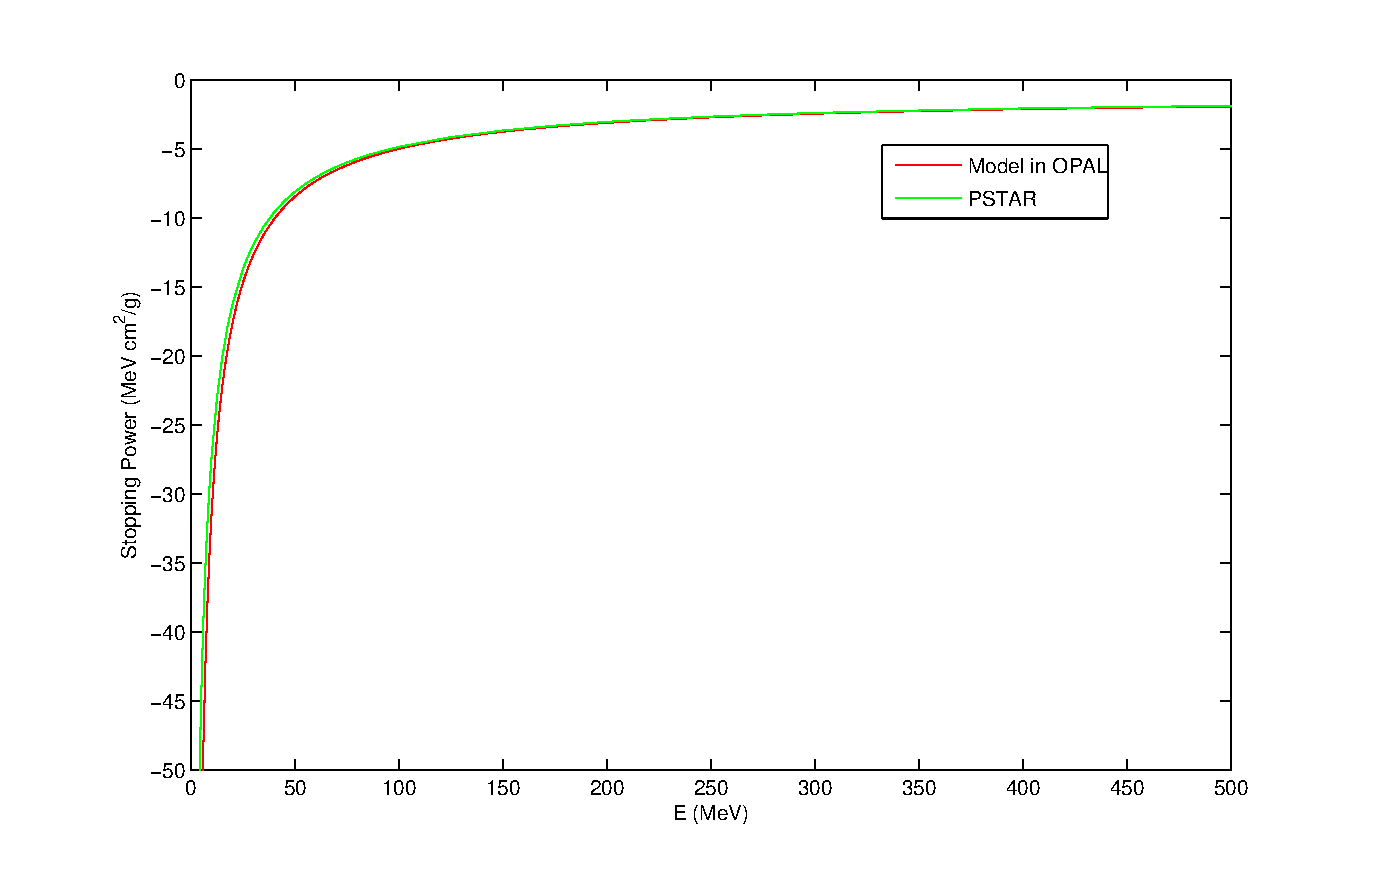
\includegraphics[width=0.5\textwidth]{figures/partmatter/dEdx}
\end{center}
\caption{The comparison of stopping power with PSTAR. }
\label{fig:dEdx}
\end{figure}

Energy straggling: For relatively thick absorbers such that the number of collisions is large, the energy loss distribution is shown to be Gaussian in form.
For non-relativistic heavy particles the spread $\sigma_0$ of the Gaussian distribution is calculated by:
\begin{equation}
\sigma_0^2=4\pi N_Ar_e^2(m_ec^2)^2\rho\frac{Z}{A}\Delta s,
\end{equation}
where $\rho$ is the density, $\Delta s$ is the thickness.

\section{The Coulomb Scattering}
The Coulomb scattering is treated as two independent events: the multiple Coulomb scattering and the large angle Rutherford scattering.\\
Using the distribution given in Classical Electrodynamics, by J. D. Jackson, the multiple- and single-scattering distributions can be written:
\begin{equation}
\label{eq:PM}
P_M(\alpha) \;\differential \alpha=\frac{1}{\sqrt{\pi}}e^{-\alpha^2}\;\differential\alpha,
\end{equation}
\begin{equation}
\label{eq:Ps}
P_S(\alpha) \;\differential{} \alpha=\frac{1}{8 \ln(204 Z^{-1/3})} \frac{1}{\alpha^3}\;\differential{}\alpha,
\end{equation}
where $\alpha=\frac{\theta}{<\Theta^2>^{1/2}}=\frac{\theta}{\sqrt 2 \theta_0}$.

\noindent The transition point is $\theta=2.5 \sqrt 2 \theta_0\approx3.5 \theta_0$,
\begin{equation}
\label{eq:Multiple}
\theta_0=\frac{\SI{13.6}{\mega\electronvolt}}{\beta c p} z \sqrt{\Delta s/X_0} [1+0.038 \ln(\Delta s/X_0)],
\end{equation}
where $p$ is the momentum, $\Delta s$ is the step size, and $X_0$ is the radiation length.

\subsection{Multiple Coulomb Scattering}
Generate two independent Gaussian random variables  with mean zero and variance one: $z_1$ and $z_2$.
If $z_2 \theta_0>3.5 \theta_0$, start over. Otherwise,
\begin{equation}
\label{eq:Multiplex}
x=x+\Delta s p_x+z_1 \Delta s \theta_0/\sqrt{12}+z_2 \Delta s \theta_0/2,
\end{equation}
\begin{equation}
\label{eq:Multiplepx}
p_x=p_x+z_2 \theta_0.
\end{equation}
Generate two independent Gaussian random variables  with mean zero and variance one: $z_3$ and $z_4$.
If $z_4 \theta_0>3.5 \theta_0$, start over. Otherwise,
\begin{equation}
\label{eq:Multipley}
y=y+\Delta s p_y+z_3 \Delta s \theta_0/\sqrt{12}+z_4 \Delta s \theta_0/2,
\end{equation}
\begin{equation}
\label{eq:Multiplepy}
p_y=p_y+z_4 \theta_0.
\end{equation}

\subsection{Large Angle Rutherford Scattering}

Generate a random number $\xi_1$, \textit{if} $\xi_1<\frac{\int_{2.5}^\infty P_S(\alpha)d\alpha}{\int_0^{2.5} P_M(\alpha)\;\differential\alpha+\int_{2.5}^\infty P_S(\alpha)\;\differential\alpha}=0.0047$, sampling the large angle
Rutherford scattering.\\
The cumulative distribution function of the large angle
Rutherford scattering is
\begin{equation}
\label{eq:Fa}
F(\alpha)=\frac{\int_{2.5}^\alpha P_S(\alpha) \;\differential \alpha}{\int_{2.5}^\infty P_S(\alpha) \;\differential \alpha}=\xi,
\end{equation}
where $\xi$ is a random variable. So
\begin{equation}
\label{eq:alpha}
\alpha=\pm 2.5 \sqrt{\frac{1}{1-\xi}}=\pm 2.5 \sqrt{\frac{1}{\xi}}.
\end{equation}
Generate a random variable $P_3$,\\
\textit{if} $P_3>0.5$
\begin{equation}
   \theta_{Ru}=2.5 \sqrt{\frac{1}{\xi}} \sqrt{2}\theta_0,
\end{equation}
\textit{else}
\begin{equation}
       \theta_{Ru}=-2.5 \sqrt{\frac{1}{\xi}} \sqrt{2}\theta_0.
\end{equation}

The angle distribution after Coulomb scattering is shown in \figref{Coulomb}.
The line is from Jackson's formula, and the points are simulations with Matlab.
For a thickness of $\Delta s=1e-4$ $m$, $\theta=0.5349 \alpha$ (in degree).

\begin{figure}[ht!]
\begin{center}
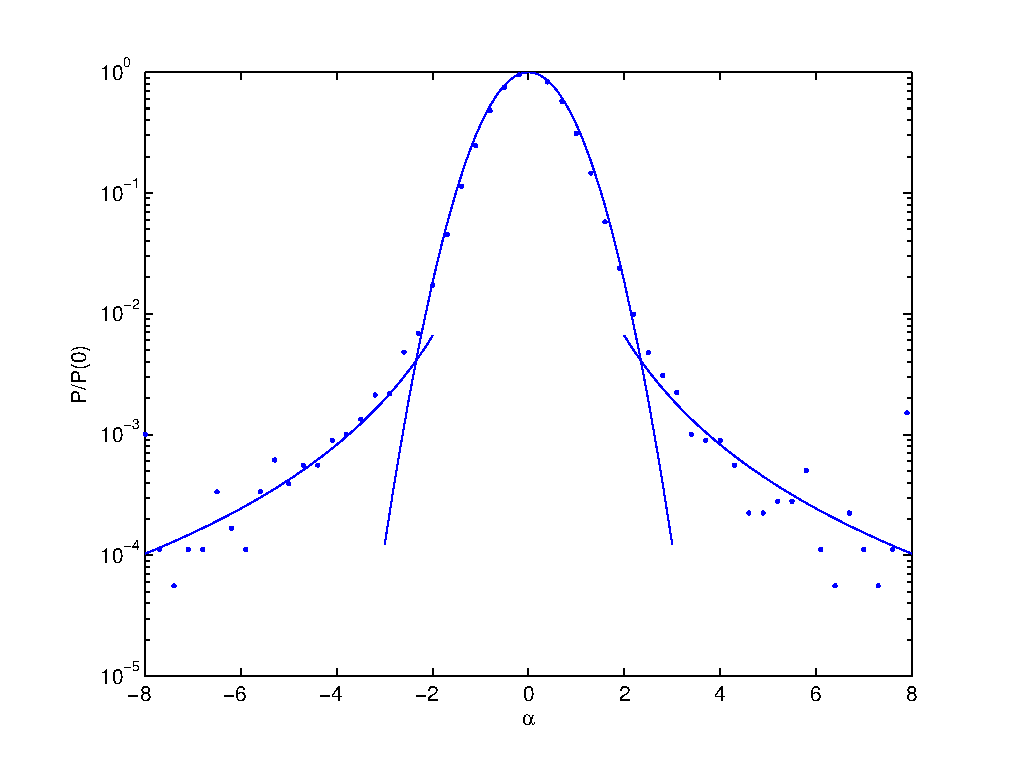
\includegraphics[width=.8\textwidth]{figures/partmatter/10steps}
\end{center}
\caption{The comparison of Coulomb scattering with Jackson's book. }
\label{fig:Coulomb}
\end{figure}

\section{The Flow Diagram of {\em CollimatorPhysics} Class in OPAL}
\begin{figure}[ht!]
\begin{center}
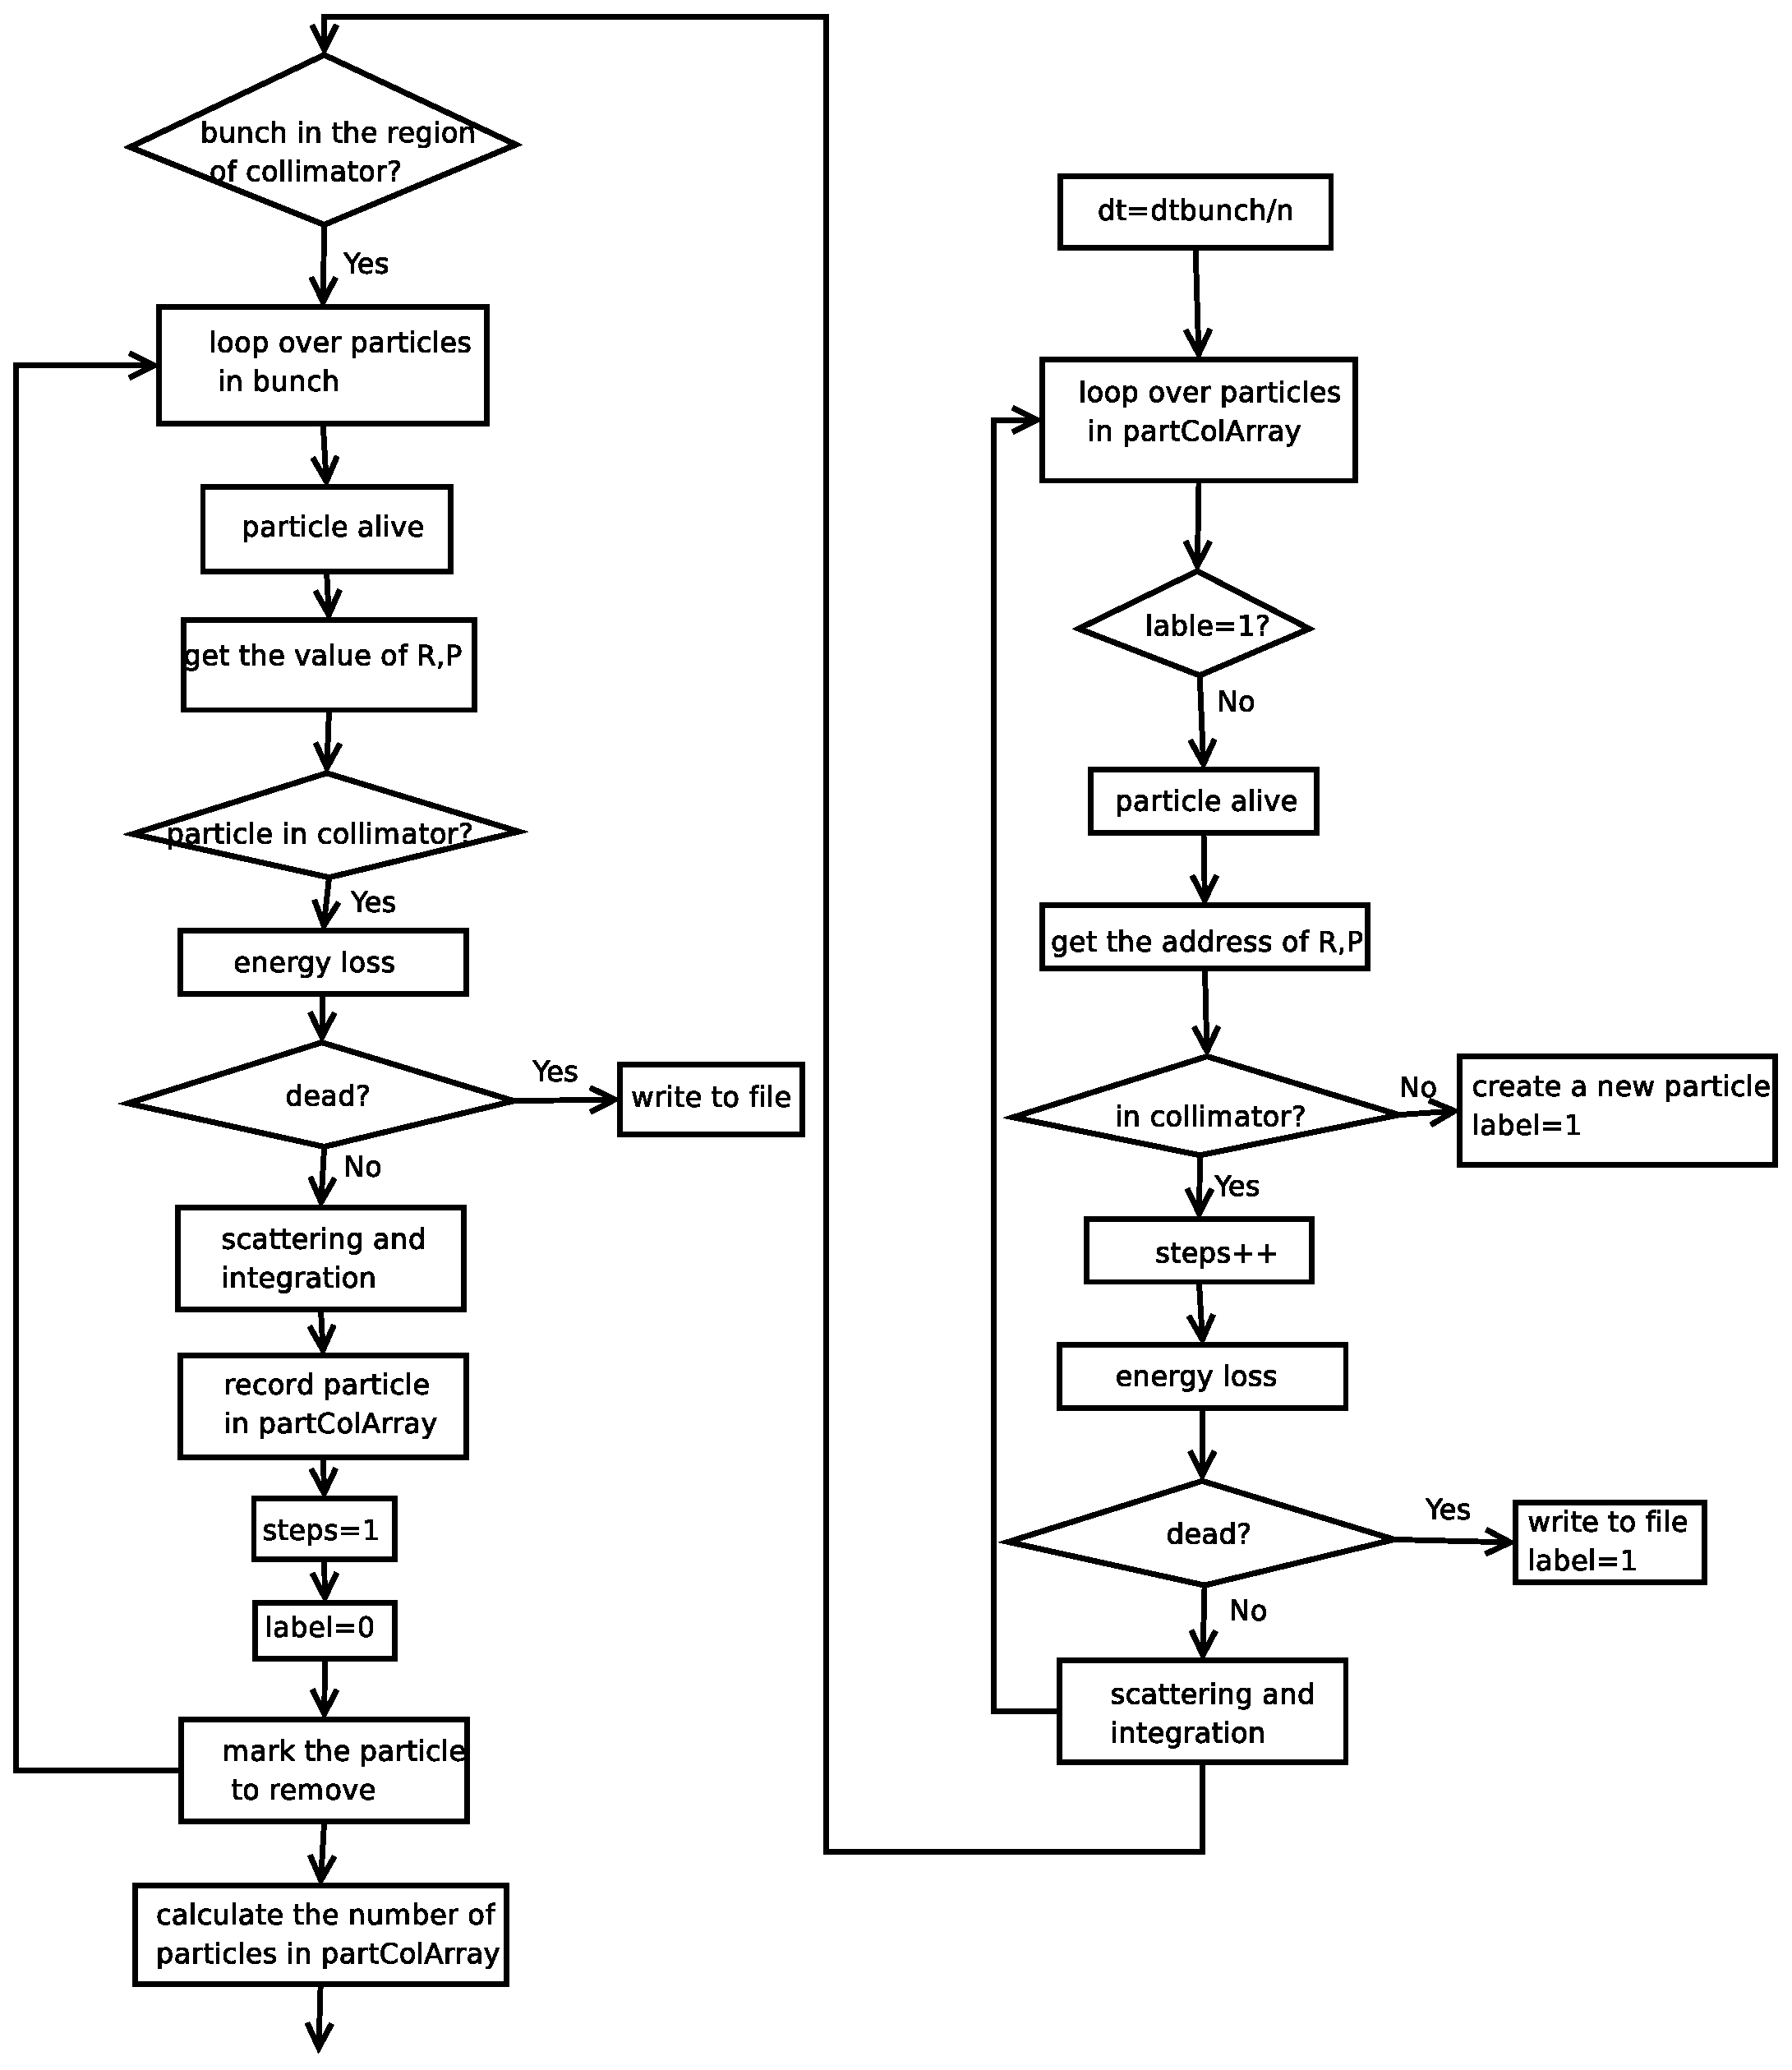
\includegraphics[width=0.8\textwidth]{figures/partmatter/diagram}
\end{center}
\caption{The diagram of CollimatorPhysics in \opal. }
\label{fig:diagram}
\end{figure}
\begin{figure}[ht!]
\begin{center}
\includegraphics[width=0.6\textwidth]{figures/partmatter/Diagram2}
\end{center}
\caption{The diagram of CollimatorPhysics in \opal (continued). }
\label{fig:diagram2}
\end{figure}
\clearpage

\subsection{The Substeps}

Small step is needed in the routine of CollimatorPhysics.

If a large step is given in the main input file, in the file \filename{CollimatorPhysics.cpp},
it is divided by a integer number $n$ to make the step size using for the calculation of collimator physics less than 1.01e-12 s. As shown
by  \figref{diagram,diagram2} in the previous section, first we track one step for the particles already in the
collimator and the newcomers, then another (n-1) steps to make sure the particles in the collimator experience the same time as the ones
in the main bunch.

Now, if the particle leave the collimator during the  (n-1) steps, we track it as in a drift and put it back to the main bunch when
finishing (n-1) steps.

\section{Available Materials in \opal}
\begin{table}[H]\footnotesize
\centering
  \caption{List of materials with their parameters implemented in \opal.}
  \label{table:Materials}
  \begin{tabular}{|c|c|c|c|c|c|c|c|c|c|}
  \hline
  \tabhead{Material     & Z    &    A         &    $\rho$  [$g/cm^3$]     &    X0      [$g/cm^2$]     &    A2    &    A3    &    A4    &    A5 & \opal Name}
    \hline
    Aluminum        &    13        &          26.98        &              2.7        &    24.01        &    4.739        &    2766        &    164.5        &    2.023E-02 & \keyword{Aluminum }\\
    %\hline
    AluminaAl2O3        &    50        &          101.96        &              3.97        &    27.94        &    7.227        &    11210        &    386.4        &    4.474e-3 & \keyword{AluminaAl2O3 }\\
    %\hline
    Copper            &    29        &      63.54        &        8.96        &    12.86        &     4.194        &    4649        &    81.13        &    2.242E-02 & \keyword{Copper}\\
    %\hline
    Graphite            &    6        &       12.0172            &           2.210    &    42.7            &    2.601        &    1701        &    1279        &    1.638E-02 & \keyword{Graphite }\\
    %\hline
    GraphiteR6710        &    6        &       12.0172            &           1.88        &    42.7            &    2.601        &    1701        &    1279        &    1.638E-02 & \keyword{GraphiteR6710}\\
    %\hline
    Titan            &    22        &      47.8        &          4.54        &    16.16        &    5.489        &    5260        &    651.1        &    8.930E-03 & \keyword{Titan }\\
    %\hline
    Air                &    7        &    14            &        0.0012        &    37.99        &    3.350        &    1683        &    1900        &    2.513E-02 & \keyword{Air }\\
    %\hline
    Kapton            &    6        &    12            &    1.4            &    39.95        &    2.601        &    1701        &    1279        &    1.638E-02 & \keyword{Kapton }\\
    %\hline
    Gold                &    79        &    197            &    19.3            &    6.46            &    5.458        &    7852        &    975.8        &    2.077E-02 & \keyword{Gold }\\
    %\hline
    Water            &    10        &    18            &    1            &    36.08        &    2.199        &    2393        &    2699        &    1.568E-02 & \keyword{Water }\\
    %\hline
    Mylar            &    6.702    &    12.88            &    1.4            &    39.95        &    3.35        &    1683        &    1900        &     2.513E-02 & \keyword{Mylar }\\
    %\hline
    Berilium                 &    4        &    9.012        &    1.848        &    65.19        &    2.590        &    966.0        &    153.8        &     3.475E-02 & \keyword{Berilium }\\
    %\hline
    Molybdenum                &    42        &    95.94        &    10.22        &    9.8            &    7.248        &    9545        &    480.2        &     5.376E-03 &  \keyword{Molybdenum}\\
    \hline
    \end{tabular}
\end{table}



\section{Example of an Input File}

\examplefromfile{examples/particlematterinteraction.in}

FX5 is a slit in x direction, the  \keyword{APERTURE} is \textbf{POSITIVE}, the first value in  \keyword{APERTURE} is the left part, the second value is the right part.
FX16 is a slit in y direction,  the  \keyword{APERTURE} is \textbf{NEGATIVE}, the first value in  \keyword{APERTURE} is the down part, the second value is the up part.

\section{A Simple Test}
A cold Gaussian beam with $\sigma_x=\sigma_y=5$ mm.
The position of the  collimator is from 0.01 m to 0.1 m, the half aperture in y direction is $3$ mm.  \figref{longcoll}
shows the trajectory of particles which are either absorbed or deflected by a copper slit. As a benchmark of the collimator model in \opal, \figref{Espectrum} shows the energy spectrum  and angle deviation at z=0.1 m after an elliptic collimator.
\begin{figure}[ht!]
\begin{center}
\includegraphics[width=0.8\textwidth]{figures/partmatter/longcoll6}
\end{center}
\caption{The passage of protons through the collimator. }
\label{fig:longcoll}
\end{figure}

\begin{figure}[ht!]
\begin{center}
\includegraphics[width=0.8\textwidth]{figures/partmatter/spectandscatter}
\end{center}
\caption{The energy spectrum and scattering angle at z=0.1 m}
\label{fig:Espectrum}
\end{figure}

%----------- Footer control ------------------
\ifthenelse{\boolean{FullOPALManual}}
{
  %do nothing
}
% else (for individual document creation)
{
\appendix
\printbibliography
\end{document}
}
%---------------------------------------------            % ch 18

%opal-map
\ifthenelse{\boolean{ShowMap}}{
  \chapter{\opal Flavours}
\label{sec:opalFlavours}
\index{opalFlavours}

\section{\opalt}
\opalt is a fully three-dimensional program to track in time, relativistic particles taking into account space charge forces, self-consistently in the electrostatic approximation, and short-range longitudinal and transverse wake fields (available in Version 1.1). \opalt  is one of the few
codes  that is implemented using a parallel programming paradigm from the ground up. This makes \opalt indispensable for
high statistics simulations of various kinds of existing and new accelerators. It has a comprehensive set of beamline
elements, and furthermore allows arbitrary overlap of their fields, which gives \opalt a capability
to model both the standing wave structure and traveling wave structure. Beside IMPACT-T it is the only code making use of
space-charge solvers based on an integrated Green \cite{qiang2005} function to efficiently and accurately treat beams with
large aspect ratio, and a shifted Green function to efficiently treat image charge effects of a cathode \cite{fubiani2006,qiang2006-2}. 
For simulations of particles sources i.e. electron guns \opalt uses the technique of  energy binning in the electrostatic space-charge calculation to model beams with large
energy spread. In the very near future a parallel Multi Grid solver taking into account the exact geometry will be implemented.  

\subsection{Integration of the Equation of Motion}
\opalt integrates the relativistic Lorentz equation
\begin{equation}
F(\vec{x},\vec{v},t) = m_0 \frac{\gamma \vec{v}}{dt} =   \frac{q}{e}[\vec{E}_{ext} + \vec{E}_{sc} + \vec{v} \times (\vec{B}_{ext} + \vec{B}_{sc})]
\end{equation}
where $\gamma$ is the relativistic mass factor and $\vec{E}$  and $\vec{B}$ are abbreviations for $\vec{E}(\vec{x},\vec{v},t)$ and $\vec{B}(\vec{x},\vec{v},t)$
respectively. \latermore .

%    NEED WORK ADA    
%\begin{equation}
%\vec{x}_{n+1/2} = \vec{x}_{n} + \frac{1}{2}\vec{v}_{n-1/2}\quad (= \vec{x}_{n} + \frac{\Delta t}{2} \frac{\vec{\beta}_{n-1/2}\gamma_{n-1/2}}{\gamma_{n-1/2}})
%\end{equation}

%Update the momenta using the $D_1$ algorithm as described in Birdsall and Langdon's book.        
                                                                                
%\begin{equation}                                                                                                                                                                                                  
%    \vec{v}_{n+1/2} = \frac{1}{2} \overline{\vec{a}_{n}}   \Delta t +  R \cdot (\vec{v}_{n-1/2} + \frac{1}{2} \overline{\vec{a}_{n}}  \Delta t)                                         
%\end{equation}
%  
%                                                                                                                                                                                                                
%         where the operator $R$ effects a rotation through angle $-2\tan^{-1}(\vec{\Omega} \Delta t/2)$ where $\vec{\Omega} = Q \vec{B}_{n}/(m_{e} c)$.                                 
%        $R$ can be written as                                                                                                                                                                     
%        \begin{equation}                                                                                                                                                                                                    
%         R = \frac{(1 - \Theta^2) I + 2  \Theta \Theta^{T} - 2  \Theta \times I }{1+\Theta}                                                                              
%        \end{equation}                                                                                                                                                                                              
%        where $\vec{\Theta} = \vec{\Omega}  \Delta t/2 $ and $I$ is the unit tensor.                                                                                                         
%      


\subsection{Space Charge}
\label{sec:opalFlavours:spacecharge}
\index{SpaceCharge}
Space-charge effects will be included in the simulation by specifying a field solver described in Section \ref{sec:fieldsolver} and using the solver in the
track command described in Section \ref{sec:track}. 
By default, the code does not assume any symmetry i.e. full 3D. In the near future it is planed to implement also a slice (2D) model.
This will allow the use of less numbers of macro-particles in the simulation which reduces the computational time
significantly. 

The space-charge forces are calculated by solving the 3D Poisson equation with open boundary conditions
using a standard or integrated Green function method. The image charge effects of the conducting cathode are also
included using a shifted Green function method. If more than one Lorentz frame is defined, the total space-charge forces are then the summation of contributions from all Lorentz frames. \latermore

\subsubsection{FFT Based Particle-Mesh (PM) Solver}
 \latermore

%    NEED WORK ADA    
%The Particle-Mesh (PM) \cite{Hockney} solver is one of the oldest improvements over the PP solver. Still one of the best references is the book by R.W.~Hockney \& J.W.~Eastwood \cite{Hockney}. 
%The PM solver introduces a discretization of space. The rectangular computation domain $\Omega:=[-L_x,L_x]\times[-L_y,L_y]\times[-L_t,L_t]$, just big enough to include all particles, is segmented into a regular mesh of $M=M_x\times M_y\times M_t$ grid points. 


%In order to obtain  ${\cal M}_2$ in Equation (\ref{eq:splitOper1}) we must solve Poisson's equation, 
%where $\rho$ stands for the
%charge density and $\phi$ for the scalar electrostatic potential:
%\begin{equation}\label{Poisson}
%\nabla^2 \phi(\vec{q}) = - \frac{\rho(\vec{q})}{\epsilon_0}
%\end{equation}
%subject to open boundary conditions in all spatial directions: $\phi (\vec{q}) \rightarrow 0$ as $|\vec{q}| \rightarrow \infty$ or
%imposing periodic boundary conditions in longitudinal directions. The assumption of using an ``isolated system`` is physically 
%motivated by observing the ratio of the beam size to vacuum vessel domensions. It has the computational advantages that one can use cyclic convolution in (\ref{eq:FourierPoisson}).
%The computational domain $\Omega \subset \R^3$ is simply connected and has a cylindrical 
%or rectilinear shape.
%The corresponding integral equation reads:
%\begin{equation}
%\phi(\vec{q}) = \dis\int\limits_\Omega \, G(\vec{q} - \vec{q}^\prime) \,\rho (\vec{q'}) \,d \vec{q}^\prime , \;\;\Omega \subset \R^3 
%\end{equation}
%where $G$ is the Green's function which gives the response to a unit source term. In 3D we have
%\begin{equation}
%G(\vec{q}-\vec{q}^\prime) = \dis\frac{1}{4 \pi \,|\vec{q} - \vec{q}^\prime|} \,.
%\end{equation}
%The electric field then follows from the electrostatic potential
%\begin{equation}\label{Electric}
%\vec{E} = - \nabla \phi.
%\end{equation}

%The charges are assigned from the particle positions in continuum, onto the grid using 
%one of two available interpolation schemes: cloud in cell (CIC) or nearest grid point (NGP). 
%Then the Poisson equation is solved on the mesh and the electric field at the particle positions is obtained by 
%interpolating back from the mesh. The use of the convolution theorem to solve the discretized Poisson 
%equation \eqref{Poisson} on the grid can dramatically improve performance. 

%Let $\Omega^D$ be spanned by a mesh of $l \times n \times m$ with $l= 1 \dots M_x$, $n= 1\dots M_x$ and $m= 1 \dots M_t$.
%The solution of the discretized Poisson equation with $\vec{k}=(l,n,m,)$
%\begin{equation}\label{eq:DiscretizedPoisson}
%\nabla^{2} \phi^D(\vec{k}) = - \frac{\rho^D(\vec{k})}{\epsilon_0}, \vec{k} \in \Omega^D.
%\end{equation}
%$\phi^D$ then is given by convolution with the appropriate discretized Green's function $G_D$: 
%\begin{equation}
%\phi^D = \rho^D * G^D.
%\end{equation}
%In Fourier space (hats) the convolution becomes a simple multiplication, with
%\[
%G(\vec{q})=\frac{1}{4\pi}\frac{1}{|\vec{q}|}\longrightarrow  \widehat{G}(\vec{k})=-\frac{1}{4\pi}\frac{1}{|\vec{k}|^2}
%\]
%and we get: 
%\begin{equation}\label{eq:FourierPoisson}
%\widehat{\phi}^D = \widehat{\rho}^D \cdot \widehat{G}^D.
%\end{equation}
%Thus, the convolution sum is converted to a single multiplication at the cost of a Fourier transform. Fortunately, Fast Fourier Transform (FFT) on the mesh is a very fast and accurate method
%of transforming mesh-defined quantities to Fourier space. It needs $\mathcal{O}$($M\log M$) computational effort, so that, together with the interpolations, an overall scaling of $\mathcal{O}$($N+M\log M$) is achieved.

%In order to have good spatial resolution, small grid sizes are often necessary, which again require a 
%large number of particles. Therefore, both the grid size $M$ and the particle number $N$ 
%are limiting factors. 
%The PM Solver Algorithm is summarized in the following algorithm: 
%\begin{tabbing}
%{\bf PM Solver Algorithm}\\
%\quad $\triangleright$ Assign particle charges $q_i$ to nearby mesh points to obtain $\rho^D$ \\
%\quad $\triangleright$ Use FFT on $\rho^D$ and $G^D$ to obtain $\widehat{\rho}^D$ and $\widehat{G}^D$ \\
%\quad $\triangleright$ Determine $\widehat{\phi}^D$ on the grid using $\widehat{\phi}^D = \widehat{\rho}^D \cdot \widehat{G}^D$ \\
%\quad $\triangleright$ Use inverse FFT on $\widehat{\phi }^D$ to obtain $\phi^D$ \\
%\quad $\triangleright$ Compute $\vec{E}^D= -\nabla \phi^D$\footnote{using a second order finite difference method} \\
%\quad $\triangleright$ Interpolate $\vec{E(\vec{q})}$ at particle positions $\vec{q}$ from $\vec{E}^D$  \\
%\end{tabbing}
%\subsubsection{Open and Periodic Boundary Conditions}
%In order to meet open boundary conditions and to remove the intrinsic periodicity of the FFT, the grid size needs to be doubled in all spatial dimensions and the charge distribution is located at only one octant. The charge distribution is set equal to zero elsewhere. If the potential is then calculated in the entire enlarged region, the correct potential for an isolated system is obtained in the `physical' octant. This is referred to as the `Hockney Trick' \cite{Hockney}. For periodic boundary conditions in the longitudinal direction, the Hockney trick is applied to the transverse directions only.
%The main drawback of this method is its high storage requirement. However, using symmetries one is 
%able to bound the required storage to $2N_g$ where $N_g$ is the grid size used in the physical
%region of the calculation (see \cite{Hockney} on p. 213). 
\subsubsection{Interpolation Schemes}
 \latermore

%\label{sec:interpol}
%Both charge assignment and electric field interpolation are related to the interpolation 
%scheme used. A detailed discussion is given in~\cite{Hockney}. 
%If $e_i$ is the charge of a particle, we can write the density at mesh point $\vec{k}_m$ as 
%\begin{equation}\label{eq:discRho}
%\rho(\vec{k}_m)^D = \sum_{i=1}^N e_i\cdot W(\vec{q}_i,\vec{k}_m), ~ m=1\dots M
%\end{equation}
%where $W$ is a suitably chosen weighting function (with local support).
%The simplest scheme is the nearest grid point (NGP) method, where the total particle charge is assigned to 
%the nearest grid point and the electric field is also evaluated at the nearest grid point. A more 
%elaborate scheme is called cloud in cell (CIC). It assigns the charge to the $2^d$ nearest grid points and 
%also interpolates the electric field from these grid points. The assigned density changes are continuous when 
%a particle moves across a cell boundary, although the first derivative is discontinuous. A schematic of the 
%CIC interpolation scheme is shown in Figure \ref{CIC} for the two-dimensional case.
%%total momentum consered. errors small at large particle separations. charge assignement schould vary smoothly as particle position changes.
% \begin{figure}
% \begin{center}
%% \includegraphics[width=0.75\linewidth]{\figdir/cic.eps}
% \caption[CIC interpolation scheme]{\label{CIC} \it CIC interpolation scheme.}
% \end{center}
% \end{figure} 

\subsubsection{Multigrid Based Solver}
This is subject to a ETH masters thesis started in February 2008, more information as the work
progresses.
\subsubsection{Energy Binning}
The beam out of a cathode or in a plasma wake field accelerator can have a large energy spread.
In this case, the static approximation using one Lorentz frame might not be sufficient. Multiple
Lorentz frames  can be used so that within each Lorentz frame the energy
spread is small and hence the electrostatic approximation is valid. 
 \latermore


\subsection{Wake Fields}
Longitudinal and transverse wake fields will be available in Version 1.1.

\subsection{Multiple Species}
In the present version only one particle species can be defined (Section \ref{sec:physics}), however 
due to the underlying general structure the implementation of a true multi species version of \opal is 
trivial. 

\subsection{Field Maps}
\label{sec:fieldmaps}
The file format used for the field maps is derived from the  {\em T7} file format as produced by Superfish~\cite{superfish}. A valid field map consists of a few header lines and a rest representing regularly spaced interpolation points either in 1D, 2D or 3D. In the case of 2D and 3D field maps the fields at a given position are calculated by linear interpolation from the nearest grid points. In the case of 1D field maps a Fourier transformation is used to calculate the longitudinal derivatives of the on-axis field. From these the fields at any position in space are calculated.

At the beginning of the first line information of the kind of field map has to be provided in form of a string. This can either be

\begin{description}
\item[1DElectroStatic]
if the file describes a 1D electrostatic field map. 1D field maps are described by the on-axis field.\\
Not implemented yet.
\item[1DMagnetoStatic]
if the file describes a 1D magnetostatic field map.\\
Not implemented yet.
\item[1DProfile1]
if the file contains Enge coefficients which describe the fringe field of an element. From these the correct field at any position is calculated. This type of field map is special in the sense that the class processing these files doesn't return the actual field at a position but rather the on-axis field profile and its first and second derivative. The classes (elements) supporting this kind of field map have to deal with this appropriately. For the user this has no consequences but these fieldmaps can be used as any other fieldmap. The reason for these internal differences lies in the way how the fields have to be computed for the different elements.
\item[1DProfile2]
if the file describes a mid plane on-axis field profile which is processed to get the corresponding Enge coefficients. Otherwise this type is the same as 1DProfile1. 
\item[1DDynamic]
if the file describes a 1D dynamic electromagnetic field map
\item[2DElectroStatic]
if the file describes a 2D electrostatic field map. 2D field maps are described by the electromagnetic field in one half-plane.
\item[2DMagnetoStatic]
if the file describes a 2D magnetostatic field map.
\item[2DDynamic]
if the file describes a 2D dynamic electromagnetic field map.
\item[3DElectroStatic]
if the file describes a 3D electrostatic field map.\\
Not implemented yet.
\item[3DMagnetoStatic]
if the file describes a 3D magnetostatic field map.\\
Not implemented yet.
\item[3DDynamic]
if the file describes a 3D dynamic electromagnetic field map.\\
Not implemented yet.
\end{description}
In the case of the 1DDynamic, 1DMagnetoStatic and the 1DElectroStatic field maps one finds in addition one integer number describing the number of Fourier coefficients to be used in the calculation of the derivative of the on-axis field. 

In the case of 2D and 3D field maps an additional string has to be provided describing the orientation of the field map. For 2D field maps this can either be 
\begin{description}
\item[XZ]
if the primary direction is in z direction and the secondary in r direction.
\item[ZX]
if the primary direction is in r direction and the secondary in z direction.
\end{description}
For 3D field maps this can be
\begin{description}
\item[XYZ]
if the primary direction is in z direction, the secondary in x direction and the tertiary in y direction
\item[YXZ]
if the primary direction is in z direction, the secondary in y direction and the tertiary in x direction
\item[ZYX]
if the primary direction is in x direction, the secondary in z direction and the tertiary in y direction
\item[YZX]
if the primary direction is in x direction, the secondary in y direction and the tertiary in z direction
\item[XZY]
if the primary direction is in y direction, the secondary in x direction and the tertiary in z direction
\item[ZXY]
if the primary direction is in y direction, the secondary in z direction and the tertiary in x direction
\end{description}

Each line after the header corresponds to a grid point of the field map. This point can be referred to by two indices in the case of a 2D field map and three indices in the case of a 3D field map respectively. Each column describes either $E_z,\; E_r,\; B_z,\; B_r\; \text{or}\;H_t$ in the 2D case and $E_x, E_y, E_z,\; B_x,\; B_y,\;\text{or}\; B_z$ in the 3D case.

By primary, secondary and tertiary direction is meant the following, see also Figure~\ref{fig:order1} and Figure~\ref{fig:order2}:
\begin{itemize}
\item
the index of the primary direction increases the fastest, the index of the tertiary direction the slowest. 
\item
the order of the columns is accordingly: if the z direction in an electrostatic field map is the primary direction then $E_z$ is on the first column, $E_r$ on the second. For all other cases it's analogous.
\end{itemize}

\begin{figure}[ht]
  \begin{center}
    \includegraphics[origin=bl,height=40mm,angle=0]{./figures/Fieldmaps/order-1.pdf}
    \caption{2D field map with primary direction corresponding to the longitudinal, secondary direction to the transverse direction}
    \label{fig:order1}
  \end{center}
\end{figure}

\begin{figure}[ht]
  \begin{center}
    \includegraphics[origin=bl,height=40mm,angle=0]{./figures/Fieldmaps/order-2.pdf}
    \caption{2D field map with primary direction corresponding to the transverse, secondary direction to the longitudinal direction}
    \label{fig:order2}
  \end{center}
\end{figure}

For the 2D dynamic case in XZ orientation there are four columns: $E_z$, $E_r$, $H_t$ and an unused column in this order. In the other orientation the first and the second column and the third and fourth column are swapped.

On the second line of the header of a 1D, 2D or 3D field map the beginning and the end of the electromagnetic field relative to the physical element in primary direction is written (in centimeters!). Also written on the second line is the number of grid points minus 1, corresponding to the number of spacings.
On the third line is the frequency. For static cases this line is omitted.

The fourth line corresponds to the second line but in secondary direction and the fifth accordingly for the tertiary direction. In the case of a 1D or 2D the fifth line is omitted since there is no tertiary direction.

On the sixth line follows the first line with field values as described above.

Even though there is no secondary direction in the 1D case the header of a 1D field map is equal to its 2D equivalent: the elements can be provided with a boolean attribute FAST which has only an effect in conjunction with a 1D field map. The code then generates internally a 2D field map and the field strengths are interpolated as in the case of 2D and 3D field maps instead of being calculated using the Fourier coefficients. The fourth line determines the transverse dimension and the grain size of the produced mesh.

\noindent Example of a 2D dynamic field map:
\begin{verbatim}
2DDynamic XZ
-3.0 51.0 4121
1498.953425154
0.0 1.0 75
  0.00000e+00  0.00000e+00  0.00000e+00  0.00000e+00
  4.36222e-06  0.00000e+00  4.36222e-06  0.00000e+00
  8.83270e-06  0.00000e+00  8.83270e-06  0.00000e+00
  .
  . (313'266 lines)
  .
  1.32490e-05  0.00000e+00  1.32490e-05  0.00000e+00
  1.73710e-05  0.00000e+00  1.73710e-05  0.00000e+00
  2.18598e-05  0.00000e+00  2.18598e-05  0.00000e+00
\end{verbatim}
In this example the field map goes from $-3$~cm to $51$~cm using 4122 grid points in longitudinal direction (in local coordinates thus if ELEMEDGE=0.069 [m] then the field begins at $0.066$~m) and from $0$~cm to $1$~cm using 76 grid points in transverse direction (radius). The frequency is $\sim 1.5$~GHz. From line 5 to the end of the file the first column are the values for $E_z$, in the second for $E_r$, in the third for $B_z$ and in the last column for $H_t$.

The field maps {\bf 1DProfile1} and {\bf 1DProfile2} are different from the rest since no actual fields are stored but a profile. They are used to represent the fringe fields of various elements. The fields have to be calculated using Enge functions \cite{enge} The fields calculated from this kind of field map depends on the kind of element in which they are used. Type 1 stores the coefficients of the Enge function whereas the type 2 stores the profile itself. From this profile the coefficients are calculated by solving a least-square equation. 

On the first line after the string describing the type of field map two integer numbers and a floating point number follow. The first integer number describes the number of Enge coefficients to be used for the entry fringe field, the second the equivalent for the exit fringe field. The floating point number specifies the gap height. On the second line the first value describes the beginning of the entry fringe field (in local coordinates; corresponds to {\sl zbegin\_entry} in Figure~\ref{fig:fringefields}), the second the origin of the Enge polynomial, the third the end of the fring field ({\sl zend\_entry}). The last number of this line is only used in Profile2 and specifies the number of grid points minus 1. The third line looks identically but the last value on this line is not used yet. The values on this line correspond to {\sl zbegin\_exit, origin of Enge function} and {\sl zend\_exit} in Figure~\ref{fig:fringefields}. The following lines are the coefficients of the Enge function in the case of 1DProfile1 and the profile in 1DProfile2.

\begin{figure}[ht]
  \begin{center}
    \includegraphics[origin=bl,height=100mm,angle=0]{./figures/Fieldmaps/profile-1.pdf}
    \caption{The profile of a rectangular bend and its corresponding design path.}
    \label{fig:fringefields}
  \end{center}
\end{figure}

\noindent Example of a 1D profile type 2:
\begin{verbatim}
1DProfile2 5 5 1.5
-5.5 -1.0 3.5 346
21.3819 25.8819 30.3819 1
0
3.79019e-05
0.000120199
.
. (344 lines)
.
0.000282913
9.84338e-05
0
\end{verbatim}
\leftpointright As a general warning: be wise when you choose the type of field map to be used! The following three pictures show the longitudinal phase space after three gun simulations using different types of field maps. In the first picture, Figure~\ref{figure_1ddynamic_step82}, we used a 1D field map which stores a sampling of the electric field in longitudinal direction, $E_z$. From these values $E_z$, $E_r$ and $B_t$ off-axis are calculated resulting in a smooth field. All field maps we used are made of the same solution file from a Poisson/Superfish simulation.
\begin{figure}
  %
  \begin{center}
  \includegraphics[origin=bl,height=80mm,angle=0]{./figures/Fieldmaps/1DDynamic_step82.png}
  %
  \caption{\label{figure_1ddynamic_step82}
    The longitudinal phase space after a gun simulation using a 1D field map (on-axis field) of the gun.
  }
  %
  \end{center}
%
\end{figure}

In Figure~\ref{figure_1ddynamic_fast_step82} we used the same on-axis field map as in the first but we used the FAST switch which constructs a 2D field map from the on-axis field maps. Between the grid points the fields are calculated using a linear interpolation. Here we see a structure which can be influence using more grid points in transverse direction.
\begin{figure}
  %
  \begin{center}
  \includegraphics[origin=bl,height=80mm,angle=0]{./figures/Fieldmaps/1DDynamic_fast_step82.png}
  %
  \caption{\label{figure_1ddynamic_fast_step82}
    The longitudinal phase space after a gun simulation using a 1D field map (on-axis field) of the gun in combination with the FAST switch.
  }
  %
  \end{center}
%
\end{figure}
In the last picture, Figure~\ref{figure_2ddynamic_step82}, we generated directely a 2D field map from the solution file of Poisson/Superfish. Here we could observe two different structures: first the fine structure stemming from the linear interpolation and secondly a much stronger structure of unknow origin.
\begin{figure}
  %
  \begin{center}
  \includegraphics[origin=bl,height=80mm,angle=0]{./figures/Fieldmaps/2DDynamic_step82.png}
  %
  \caption{\label{figure_2ddynamic_step82}
    The longitudinal phase space after a gun simulation using a 2D field map of the gun generated by Poisson/Superfish.
  }
  %
  \end{center}
%
\end{figure}


\subsection{Field Maps from the Femaxx 3D Eigenmode Solver}

Electromagnetic field maps for beam dynamics calculations originate from a number of different
electromagnetic solvers, e.g. Superfish and similar codes.
%%
%%
Here, we describe the current status of work in progress which will, eventually,
allow the usage of field maps that have been computed with the femaxx $3$-dimensional
electromagnetic eigenmodal solver \cite{bib:arbenzetal2001,bib:arbenzetal2006}.
%%
%%
The femaxx code computes electromagnetic eigenmodes of resonant cavities of
arbitrary $3$-dimensional shape and boundary conditions.
%%
Unlike Superfish and similar $2$-dimensional codes, femaxx is not restricted in the
kind of geometry it can model. It is therefore possible to consider arbitrary
shapes and their inclusion in beam dynamics and particle tracking calculations.
%%
%%
Given a mesh of a $3$-dimensional geometry femaxx computes eigenomdal field
decompositions.
%%
The user then specifies sampling locations for the electromagnetic eigenfields.
%%
At present, sampling locations are specified in terms of a cylinder shape,
i.e. the user indicates the cylinder axis, the radial cylinder vector and 
the number of sampling locations in axial, radial and azimuthal directions.
%%
Once the eigenmodal solution has been computed the fields are sampled at
these locations and stored in the T7 file format, for subsequent use in \opal.
%%
Considerable effort has been spent for the validation and benchmarking of
beam dynamics calculations based on T7 field maps computed with femaxx.
%%
A pillbox cavity, i.e. a cylinder shape with a radius $r = 4.7$cm and
height $h = 3$ cm, has been chosen for benchmarking purposes,
due to the availability of an analytical solution.
%%
The analytical resonance frequency of the dominant mode is $2.441$ GHz.
%%
%%
We have compared two cases with \opal: (1) The analytical solution has been
sampled within a cylinder volume, stored into a T7 file and used in an \opal
run; (2) the same pillbox shaped geometry has been discretization into tetrahedra
and the eigenmodal fields were calculated with femaxx.
%%
These two cases were then compared, resulting in the following conclusions:
%%
(1) Using a relatively coarse mesh with some $110'000$ tetrahedra, the difference
between the analytical and the numerical solution was usually smaller than
$1$ percent.
%%
(2) Using an adaptively refined mesh, the difference between analytical and
numerical solutions decreased below $1$ pro mille. The mesh is shown
in the figure (\ref{figure_pillbox_adaptively_refined_mesh}).
%%
(3) It is thereofore imperative to usa a tetrahedral mesh which has been
refined around the beam axis. It is definitely more efficient to use local
refinement, based on physical argument, than simply refine the complete
mesh in a uniform manner.
%%


We are now working towards benchmarking more complicated shapes in order to
assess requirements w.r.t to meshes and modeling geometry so that we
achieve the same or better accuracy as has been obtained from field
maps that were computed with Superfish like solvers based on azimuthal symmetry.

\begin{figure}
  %
  \begin{center}
  \includegraphics[origin=bl,width=80mm,angle=0]{./figures/adaptivePillboxMesh.pdf}
  %
  \caption{\label{figure_pillbox_adaptively_refined_mesh}
    We show the discretization of a pillbox shaped cavity geometry
        into a tetrahedral mesh. The mesh has been adaptively
        refined so that the region around the cylinder axis is
        decomposed into smaller tetrahedra than those which are
        further away from the axis.
  }
  %
  \end{center}
%
\end{figure}

\clearpage
\subsection{Output}
The data is stored in the H5Part file-format (\url{http://h5part.web.psi.ch/}) and can be analysed
using the H5PartRoot (\url{http://amas.web.psi.ch/tools/H5PartROOT/index.html}). The frequency 
of the data output (phase space and some statistical quantities) can be set using the \secref{\texttt{OPTION} statement}{option}, 
statement and the flag PSDUMPFREQ. The file is named like in input file but the extension is {\tt .h5}. 

\begin{figure}[ht]
 \begin{center}
 \includegraphics[width=0.45\linewidth,angle=0]{figures/H5rootPicture1}
  \includegraphics[width=0.45\linewidth,angle=0]{figures/H5rootPicture2}
  \caption{H5PartROOT enables a variety of data analysis and post processing task on \opal data}
  \label{fig:h5root1}
 \end{center}
\end{figure}



\begin{figure}[ht]
 \begin{center}
   \includegraphics[width=.9\linewidth,angle=0]{figures/H5rootPicture3}
  \caption{Example of a longitudinal phase space shown with H5PartROOT}
  \label{fig:h5root2}
 \end{center}
\end{figure}



An ASCII file with statistical beam 
parameters is stored in a {\tt .stat} file. An SDDS file output is in preparation.

\section{\opalcycl}
\label{sec:opalcycl}
\index{opalFlavours}

\subsection{Introduction}

\opalcycl is a fully three-dimensional parallel beam dynamics simulation program dedicated to future high intensity cyclotrons 
which is capable of doing single particle tracking for conventional orbit designs on single computation node and 
multiple particles tracking in a parallel environment which takes into account both space charge effects 
 
For the first time in the cyclotron community, \opalcycl has the capability to track multiple bunches simultaneously
and take into account the beam-beam effects of the radial neighboring bunches( we call it neighboring bunch effects for short)
by using a self-consistent numerical simulation model.

According to the number of particles (defined by argument \texttt{NPART} in \texttt{BEAM}, see Section \ref{sec:beam}) , 
\opalcycl works in the following three modes automatically:

\begin{description}

\item[Single Particle Tracking mode]

  In this mode, only one particle is tracked, either with acceleration or not.  Working in this mode, \opalcycl
  can be used as a tool during the preliminary design phase of a cyclotron.  

  The 6D parameters of a single particle in the initial local frame must be read from a file. To do this, in the \opal input file, 
  the command line \texttt{DISTRIBUTION}(See Chapter \ref{sec:distribution}) should be defined like this:
\begin{verbatim}
  Dist1: DISTRIBUTION, DISTRIBUTION=fromfile,
         FNAME="PartDatabase.dat";
\end{verbatim}
 where the file $PartDatabase.dat$ should has two lines:
\begin{verbatim}
 1
 0.001 0.001   0.001   0.001   0.001  0.001    
\end{verbatim}
The number in the first line is the total number of particles.
In the second line the data represents $x, p_x, y,$$ p_y, z, p_z$ with the reference particle 
in the local frame and the units are $m, rad,$ $ m,rad,$ $ m, rad$ respectively.

Please don't try to run his mode in parallel environment. You should believe that a single processor of the 21st centery is capable of doing
the single particle tracking.  

\item[Tune Calculation mode]

  In this mode, two particles are tracked, one with all data is set to zero is the reference particle and another one is an off-centering particle 
  which has a little shift from the other one in both $r$ and $z$ directions. Working in this mode, \opalcycl can 
  calculate the betatron oscillation frequency $\nu_r$ and $\nu_z$ for different energies to evaluate the focusing characteristics 
  for a given magnetic field.

  Like the single particle tracking mode, 
  the 6D parameters of the two particles in initial local frame must be read from a file, too.
  In the file should has three lines:
\begin{verbatim}
 2
 0.0   0.0   0.0   0.0   0.0   0.0  
 0.001 0.0   0.0   0.0   0.001  0.0    
\end{verbatim}

When the total particle number equals 2, this mode is triggered automatically.
Only the element \texttt{CYCLOTRON} in the beam line is used and other elements are omitted if any exists.

Please don't try to run his mode in parallel environment, either.


\item[Multi-bunches tracking mode]

  In this mode, large scale particles can be tracked simultaneously, either with space charge or not, 
  either single bunch or multi-bunches, either serial or parallel environment, 
  either reading the initial distribution from a file or generating a typical distribution,  
  either running from the beginning or restarting from the last step of a former simulation.

  Beacuse this is the main mode as well as the key part of \opalcycl, 
  we will describe this in detail in Section \ref{sec:opalcycl:MultiBunch}.

\end{description}  
  
Generally speaking, the following aspects may be considered for quantitatively studying high intensity beam dynamics in cyclotrons:
  \begin{itemize}
  \item large scale particles, as many as possible, which is of course limited by computer sources;
  \item measured magnetic field map or numerical calculated field with high precision;
  \item numerical integrator with high precision;
  \item powerful parallel Poisson solver with high precision and resolution;
  \item imperfection and misalignment of the machine;
  \item the influences of other factors induced by high intensity, such as beam-beam effects and weak field effects induced in the cavities. 
  \end{itemize}
  In the following sections of this chapter, some of the above issues will be described in detail for \opalcycl.

\subsection{Field Map}
\label{sec:opalcycl:fildmap}
In \opalcycl, the magnetic field is read from an ASCII type file. The field data should be stored in the cylinder coordinates frame
( because the field map on the median plane of the cyclotron is usually measured in this frame ). 

There are two possible situations. One is the real field map on median plane of the exist cyclotron machine using measurement equipment.
Limited by the narrow gaps of magnets, in most cases with cyclotrons, only vertical field $B_z$ on the median plane ($z=0$) is measured.
Since the magnetic field data off the median plane field components is necessary for those particles with $z \neq 0$, the field need to be expanded in $Z$ direction. 
According to the approach given by Gordon and Taivassalo, by using a magnetic potential and measured $B_z$ on the median plane, 
at the point $(r,\theta, z)$ in cylindrical polar coordinates, the 3$th$ order field can be written as    
\begin{eqnarray}\label{eq:Bfield}
  B_r(r,\theta, z) & = & z\frac{\partial B_z}{\partial r}-\frac{1}{6}z^3 C_r, \nonumber\\    
  B_\theta(r,\theta, z) & = & \frac{z}{r}\frac{\partial B_z}{\partial \theta}-\frac{1}{6}\frac{z^3}{r} C_{\theta}, \\     
  B_z(r,\theta, z) & = & B_z-\frac{1}{2}z^2 C_z,  \nonumber    
\end{eqnarray}
where $B_z\equiv B_z(r, \theta, 0)$ and  
\begin{eqnarray}\label{eq:Bcoeff}
  C_r & = & \frac{\partial^3B_z}{\partial r^3} + \frac{1}{r}\frac{\partial^2 B_z}{\partial r^2} - \frac{1}{r^2}\frac{\partial B_z}{\partial r} 
        + \frac{1}{r^2}\frac{\partial^3 B_z}{\partial r \partial \theta^2} - 2\frac{1}{r^3}\frac{\partial^2 B_z}{\partial \theta^2}, \nonumber  \\    
  C_{\theta} & = & \frac{1}{r}\frac{\partial^2 B_z}{\partial r \partial \theta} + \frac{\partial^3 B_z}{\partial r^2 \partial \theta}
        + \frac{1}{r^2}\frac{\partial^3 B_z}{\partial \theta^3},  \\
  C_z & = & \frac{1}{r}\frac{\partial B_z}{\partial r} + \frac{\partial^2 B_z}{\partial r^2} + \frac{1}{r^2}\frac{\partial^2 B_z}{\partial \theta^2}. \nonumber
\end{eqnarray}

All the partial differential coefficients are on the median plane and can be calculated by interpolation. \opalcycl uses  Lagrange's  5-point formula.

The other situation is calculating 3D fields for interesting region numerically by creating 3D model using commercial softwares,
such as TOSCA, ANSOFT and ANSYS during the design phase of a new machine. The field should be more accurate than 
expansion approach especially at the region far away from median plane in $Z$ direction.

In the current version, we implemented the function $Cyclotron::$$getFieldFromFile()$ to read field data from 
the PSI format field file {\small{ZYKL9Z.NAR}}. We put 4 parameters at the header of the file, namely, $r_{min}$, $\Delta r$,
$\theta_{min}$ and $\Delta \theta$.
{\bfseries You should revise this function or write your own function according to the instructions in the code to match your own field
  format if it is different to the PSI format.}  
The generic interface function for both the 2D measured map and the 3D field from file will be available in a later version.\\ 

For more detail about the parameters of cyclotron, see Section \ref{sec:cyclotron}.

In the current version of \opalcycl, the RF cavities are treated as straight lines with infinitely narrow gaps
and the electric field is a $\delta$ function plus a transit time correction.
the two-gap cavity is treated as two independent single-gap cavities. the spiral gap cavity is not implemented yet.

For more detail about the parameters of cyclotron cavities, see Section \ref{sec:cavity-cycl}.

The voltage profile of a cavity gap  is read from ASCII file. Here is an example:
\begin{verbatim}
6  
0.00      0.15      2.40 
0.20      0.65      2.41 
0.40      0.98      0.66 
0.60      0.88     -1.59 
0.80      0.43     -2.65 
1.00     -0.05     -1.71 
\end{verbatim}
The number in the first line means 6 sample points and in the following lines the three values represent the normalized distance to 
the inner edge of the cavity, the normalized voltage and its derivative respectively.

\subsection{Particle Tracking and Accelerating}  

The precision of Tracking methods is vital for the entire simulation process, especially for long distance tracking jobs.
\opalcycl uses a 4th order Runge-Kutta algorithm which has high precision and is widely used in the accelerator 
community. It seeks the external magnetic field and does a field interpolation for 4 times in each time step $\tau$ .
During the field interpolation process, for an arbitrary given point the code first interpolates Formula $B_z$
for its counterpart on the median plane and then expands to this give point using (\ref{eq:Bfield}). 

After each time step $i$, the code detects whether the particle crosses any one of the RF cavities during this step.
If it does, the time point $t_c$ of crossing is calculated and the particle return back to the start point of 
step $i$. Then this step is divided into three substeps:
first, the code tracks this particle for $ t_1 = \tau - (t_c-t_{i-1})$;
then it calculates the voltage and adds momentum kick to the particle and refreshes its relativistic parameters $\beta$ and $\gamma$; 
and then trackes it for $t_2 = \tau - t_1$. 

\subsection{Space Charge Effects}  

\opalcycl uses the same IPPL module as \opalt to calculate the space charge effects (see Section \ref{sec:opalFlavours:spacecharge}).
The difference is that, in a cyclotron,
both the origin and orientation of the local Cartesian frame are changed from time to time. So the coordinates are transformed from 
the global frame to the local frame first, then the space charge fields are calculated in the local frame. 
After the space charge fields are solved, both coordinates and self electric and magnetic field are transformed back to global frame.
 
In the current version, the space charge fields are calculated once for each track step and is kept constant during this step.      

\subsection{Multi-bunches Issues}
\label{sec:opalcycl:MultiBunch}
				   
The neighboring bunches problem is motivated by the fact  for high intensity cyclotrons with small turn
separation, single bunch space charge effects are not the only contribution. Along with the increment of beam
current, the mutual interaction of neighboring bunches in radial direction becomes more and more important,
especially at large radius where the distances between neighboring bunches get increasingly small and even they
can overlap each other.One good example is PSI 590 MeV Ring cyclotron with a current of about 2mA in
CW operation and the beam power amounts to 1.2MW. A upgrade project for Ring is working in process with
the goal of 1.8 MW CW on target by replacing four old aluminum resonators by for new copper ones with peak
voltage increasing from about 0.7 MV to above 0.9 MV. After upgrade, the total turn 
number is reduced from 200 turns to less then 170 turns. 
Turn separation is increased a little bit, but still at the same order 
of magnitude as the radial size bunch. So once the beam current increases from 2 mA to 3 mA, the mutual space
charge effects between radially neighboring bunches can have significant impact on beam dynamics 
So it is important to cover neighboring bunch effects in the simulation to quantitatively study its impact on the beam dynamics.

In \opalcycl, we developed a new fully consistent algorithm of multi-bunches simulation.  We implemented two working modes, namely , 
\texttt{AUTO} and \texttt{FORCE}. In the first mode, only a single bunch is tracked and accelerated at the beginning,
until the radial neighboring bunch effects become an important factor to the bunches' beheaver. Then the new bunches will be injected automatically to 
take these effects into accout. In this way, we can save time and memory sufficiently, and more important, 
we can get higher precision for the simulation in the region where neighboring bunch effects are neglectable.
In the other mode, multi-bunches simulation starts from the injection points. This mode is appropriate for the machines in which this effects is 
unneglectable since the injection point.    

In the space charge calculation for multi-bunches, the computation region covers all bunches.
Because the energy of the bunches is quite different, it is inappropriate to use only one particle rest frame and a single Lorentz transformation any more.
So the particles are grouped into different energy bins and in each bin the energy spread is relatively small. We apply Lorentz transforming, calculate
the space charge fields and apply the back Lorentz transforming for each bin separately. Then add the field data together. Each particle has a ID number to identify 
which energy bin it belongs to.

\subsection{Input}  
All the three working modes of \opalcycl use an input file written in MAD language which will be described in detail in the following chapters.

For the  {\bfseries Tune Calculation mode}, one additional auxiliary file with the following format is needed.
\begin{verbatim}
   72.000 2131.4   -0.240  
   74.000 2155.1   -0.296  
   76.000 2179.7   -0.319 
   78.000 2204.7   -0.309 
   80.000 2229.6   -0.264 
   82.000 2254.0   -0.166 
   84.000 2278.0    0.025 
\end{verbatim}
In each line the three values represent energy, reference $P_\theta$ and reference $P_r$ for the SEO(Static Equilibrium Orbit) 
at starting point respectively and their units are $MeV,  mrad,  mrad$.

A bash script $tuning.sh$ is needed to execute \opalcycl once for each energy. 
{ \footnotesize
\begin{verbatim}
  #!/bin/bash
  rm -rf tempfile
  rm -f plotdata
  rm -f tuningresult

  exec 6<FIXPO_SEO
  N="260"
  j="1"
  while read -u 6 E1 r  pr
  # read in Energy, initil R and intial Pr of each 
  # SEO from FIXPO output
  do
  rm -rf tempfile
  echo -n j =
  echo "$j"
  echo -n energy= > tempfile
  echo -n "$E1"  >> tempfile
  echo  ";" >> tempfile

  echo -n r=  >> tempfile
  echo -n "$r" >> tempfile
  echo ";" >> tempfile

  echo -n pr= >> tempfile
  echo -n "$pr" >> tempfile
  echo  ";" >> tempfile
  # execute OPAL to calculate tuning frquency and store
  opal testcycl.in --commlib mpi --info 0|grep "Max" >>tuningresult
  j=$[$j+1]
  done
  exec 6<&-
  rm -rf tempfile

  # post porcess
  exec 8<tuningresult
    rm -f plotdata
  i="0"

  while [ $i -lt $N ]
  do
  read -u 8 a b ur1 d
  read -u 8 aa bb uz1 dd
  echo "$ur1   $uz1" >>plotdata
  i=$[$i+1]
  done

  exec 8<&-
  rm -f tuningresult
\end{verbatim}
}
To start execution, just run $tuning.sh$ which uses the input file $testcycl.in$ and the auxiliary file {\footnotesize$FIXPO\_SEO$}.
the output file is $plotdata$. Then one can plot a betatron tune diagram.

\subsection{Output}  
For the {\bfseries Single Particle Tracking mode}, the intermediate phase space data is stored in an ASCII file which can be used to
the plot orbit. The file's name is combined by input file name (without extension) and $-trackOrbit.dat$.
Another ASCII file stores the phase space data after one turn of tracking is finished. The file's name is a combination of input file name 
(without extension) and $-afterEachTurn.dat$.\\
 
For the {\bfseries Tune calculation mode}, the tunes $\nu_r$ and $\nu_z$ of each energy are stored in a ASCII file with name 
$tuningresult$.\\

For the {\bfseries Multi-bunches tracking mode}, the intermediate phase space data of all particles and some interesting parameters, 
including RMS envelop size, RMS emittance, external field, time, energy, length of path, number of bunches and 
tracking step, are stored in the H5Part file-format (\url{http://h5part.web.psi.ch/}) and can be analyzed
using the H5PartRoot (\url{http://amas.web.psi.ch/tools/H5PartROOT/index.html}). The frequency 
of the data output can be set using the \secref{\texttt{OPTION} statement}{option} and the flag PSDUMPFREQ. 
The file is named like in the input file but the extension is $.h5$. 

\section{\opalmap} \label{sec:SplitOperatorMethods}

Typically, the total Hamiltonian can be written as the sum of two parts, $H = H_{1} + H_{2}$,
which correspond to the external and space-charge contributions respectively.
Such a situation is ideally suited to multi-map
symplectic Split-Operator methods~\cite{forestall}, also known as fractional step methods \cite{SanzSerna}.
A second-order accurate algorithm for a single step is given by
\begin{equation} \label{eq:splitOper1}
{\cal M}(\tau)={\cal M}_1(\tau/2)~{\cal M}_2(\tau)~{\cal M}_1(\tau/2) + \mathcal{O}(\tau^3)
\end{equation}
where $\tau$ denotes the step size, ${\cal M}_1$ is the map corresponding
%(\ref{eq:mad9pham})
to $H_{1}$  and ${\cal M}_2$ is the map corresponding to $H_{2}$.
If desired this approach can be
easily generalized to higher order accuracy using Yoshida's
scheme. % ~\cite{yoshida}.
This is the simplest 2nd order symplectic\footnote{Products of symplectic operators are symplectic as well.} Split-Operator integration method, which first applies all external forces for the first half of one integration step, then adds the complete influence of the internal forces for one entire integration step, and then applies another half of an integration step worth of external forces.
Details following when \opalmap is implemented.









\index{opalFlavours)}
        % ch 4
  %=================================================
%=================================================
%
% WARNING: NOT USED IN opal_user_guide.tex
%
%=================================================
%=================================================

\ifdefined \buildingFullOPALManual \else


%\ifx \@buildingFullOPALManual \@empty
%\else

%\documentclass[12pt,a4paper]{report}
\documentclass[a4paper]{book}

%% does not work in Latex2Html mode
%\usepackage{hyperref}

\usepackage[T1]{fontenc}
\usepackage{url}
\usepackage{html}
\usepackage{epic}
\usepackage{eepic}
\usepackage{makeidx}
\usepackage{array}
\usepackage{times}
\usepackage{amsmath}
\usepackage{amsxtra}
\usepackage{bm}
\usepackage[thin,thinp,thinc]{esdiff}
\usepackage{etoolbox}
\usepackage{graphicx}
\usepackage{dingbat}
\usepackage{color}
\usepackage{subfig}
\usepackage{boxedminipage}
\usepackage{alltt}
\usepackage{nicefrac}
\usepackage{calc}
%\usepackage{pdfdraftcopy}             % Draft
\usepackage{tikz}
\usetikzlibrary{
  er,3d,calc,fadings,trees,positioning,arrows,chains,decorations.pathreplacing,
  decorations.pathmorphing,shapes,shapes.symbols,shapes.arrows,matrix,through,decorations.text
}

\tikzset{
  >=stealth',
  punktchain/.style={rectangle,rounded corners, draw=black, very thick,text width=10em,
                     minimum height=3em, text centered, on chain},
  line/.style={draw, thick, <-},
  element/.style={tape,top color=white,bottom color=blue!50!black!60!,minimum width=8em,
                  draw=blue!40!black!90, very thick,text width=10em, minimum height=3.5em,
                  text centered, on chain},
  every join/.style={->, thick,shorten >=1pt},
  tuborg/.style={decorate},
  tubnode/.style={midway, right=2pt}
}

\tikzstyle{material}=[draw, fill=blue!20, text width=16.0em, text centered, minimum height=1.5em]
\tikzstyle{diagramstep} = [material, text width=20em, minimum width=10em, minimum height=3em, rounded corners]
\tikzstyle{line} = [draw, thick, color=black!50, -latex']

\usepackage{booktabs}
\usepackage{xspace}
\usepackage{xstring}

\usepackage{fancyvrb}
\usepackage{rotating}
\usepackage{float}

\usepackage{tabularx}
\usepackage{longtable}
\setcounter{LTchunksize}{3}

\usepackage[section]{placeins}
\usepackage{MnSymbol}
\usepackage{microtype}
\usepackage{setspace}
\usepackage{dcolumn}

\usepackage[vmargin={3.0cm,3.0cm},
            hmargin={2.0cm,3.0cm}]{geometry}

\usepackage{upgreek}
\usepackage[binary-units=true]{siunitx}
\sisetup{exponent-product = \cdot,math-ohm=\Upomega,text-ohm=\ensuremath{\Upomega}}
\DeclareSIUnit{\clight}{c}
\DeclareSIUnit\gauss{Ga}

\usepackage{engord}
\usepackage{wasysym}
\DeclareSIUnit[number-unit-product = \,]{\permill}{\permil}

\usepackage{hyperref}
\hypersetup{
    pdftitle          = The OPAL Framework,
    pdfauthor         = {Andreas Adelmann, Achim Gsell, Valeria Rizzoglio, Christof Metzger-Kraus,
                         Yves Ineichen, Xiaoying Pang, Steve Russell, Chuan Wang, Jianjun Yang,
                         Suzanne Sheehy, Chris Rogers, Daniel Winklehner},
    pdfsubject        = User's Reference Manual,
    pdffitwindow      = true,               % page fit to window when opened
    pdfnewwindow      = true,               % links in new window
    colorlinks        = true,               % false: boxed links; true: colored links
    linkcolor         = black!80!green,     % color of internal links
    citecolor         = black!20!red,       % color of links to bibliography
    urlcolor          = blue,               % color of external links
    breaklinks        = true,
    bookmarksnumbered = true,
    plainpages        = false
}

\usepackage{ifthen}

\newif \iflinuxwindows
\linuxwindowstrue   % set this to true when building the manual on Linux or Windows
\iflinuxwindows
\usepackage{epstopdf}
\fi

\usepackage[backend=biber,
            style=phys,
            biblabel=brackets,
            maxnames=3,
            doi=true,
            isbn=true,
            url=true]{biblatex}
%---- macros ----

\renewcommand{\topfraction}{1.0}
\renewcommand{\bottomfraction}{1.0}
\renewcommand{\textfraction}{0.0}
\renewcommand{\arraystretch}{2.0}
\newenvironment{tex2html_nowrap}{}{}


\newcommand{\Newline}{\hfil \\}


\newsavebox{\ExampleBox}
\newenvironment{example}
 {\VerbatimEnvironment
  \begin{flushleft}
  \begin{lrbox}{\ExampleBox}
    \begin{minipage}{\linewidth}
  \begin{Verbatim}[frame=lines,xleftmargin=0cm,fontsize=\footnotesize,samepage=true]}
 {\end{Verbatim}
  \end{minipage}
  \end{lrbox}
  \mbox{\usebox{\ExampleBox}}
  \end{flushleft}
 }

\newenvironment{longexample}
{\Verbatim[frame=lines,xleftmargin=0mm,fontsize=\footnotesize]}
{\endVerbatim}

%\examplefromfile{filename} reads in a text file and displays it in the document.
\newcommand{\examplefromfile}[1]{
\VerbatimInput[frame=lines,xleftmargin=0mm,fontsize=\footnotesize,label=\texttt{#1}]{#1}}

%for upright d of differentials
\makeatletter
\newcount\my@repeat@count

\newcommand{\myrepeat}[2]{%
  \begingroup
  \my@repeat@count=\z@
  \@whilenum\my@repeat@count<#1\do{#2\advance\my@repeat@count\@ne}%
  \endgroup
}

\newcommand{\differential}[1]{\ifstrempty{#1}{\ES@dop\ES@difint}{\ES@dop^{#1}\ES@difint}}
\newcommand{\pdifferential}[1]{\ifstrempty{#1}{{\partial\,}}{{\partial^{#1}\,}}}

\makeatother

\newcommand{\der}[3][]{\frac{\differential{#1}#2}{\differential{}\ifstrempty{#1}{#3}{#3^#1}}}
\newcommand{\parder}[3][]{\frac{\pdifferential{#1}#2}{\pdifferential{}\ifstrempty{#1}{#3}{#3^#1}}}
\newcommand{\niceder}[3][]{\nicefrac{\differential{#1}#2}{\differential{}\ifstrempty{#1}{#3}{#3^#1}}}
\newcommand{\uglyder}[3][]{{\differential{#1}#2}/{\differential{}\ifstrempty{#1}{#3}{#3^#1}}}
\newcommand{\uglyparder}[3][]{{\pdifferential{#1}#2}/{\pdifferential{}\ifstrempty{#1}{#3}{#3^#1}}}
\newcommand{\dd}[1][]{\; \differential{#1}}
\newcommand{\primed}{^{\prime}}
\newcommand{\dprimed}{^{\prime\prime}}
\newcommand{\nprimed}[1]{^{\myrepeat{#1}{\prime}}}

%Editing Macros
\newcommand{\TODO}[1]{{\color{red}\ifthenelse{\boolean{ShowDebug}}{[TODO: #1]}{}}}



%text in gray box
\newsavebox{\fmbox}
\definecolor{lightgray}{gray}{0.95}
\newenvironment{fmpage}
   {\vspace{-1.0cm}\begin{lrbox}{\fmbox}\begin{minipage}[t]{13.5cm}\vspace{0.1cm}}
   {\vspace{-0.4cm}\end{minipage}\end{lrbox}\begin{center}\fcolorbox{black}{lightgray}{\usebox{\fmbox}}\end{center}}


% Definition new signes
\newcommand{\R}{{\mathbb R}} % real numbers
\newcommand{\Q}{{\mathbb Q}} % rational numbers
\newcommand{\Z}{{\mathbb Z}} % integer numbers
\newcommand{\N}{{\mathbb N}} % natural numbers

\newcommand{\mad}{\textsc{mad}\xspace}
\newcommand{\madnine}{\textsc{mad9}\xspace}
\newcommand{\madninep}{\textsc{mad9p}\xspace}
\newcommand{\madeight}{\textsc{mad8}\xspace}
\newcommand{\classic}{\textsc{classic}\xspace}

\makeatletter
\newcommand{\opal@impl}{\textsc{Opal}}
\newcommand{\opalt@impl}{\textsc{Opal-t}}
\newcommand{\opalcycl@impl}{\textsc{Opal-cycl}}
\newcommand{\opalmap@impl}{\textsc{Opal-map}}
\newcommand{\opalenv@impl}{\textsc{Opal-e}}

\newcommand{\opal}{\opal@impl\xspace}
\newcommand{\opalt}{\opalt@impl\xspace}
\newcommand{\opalcycl}{\opalcycl@impl\xspace}
\newcommand{\opalmap}{\opalmap@impl\xspace}
\newcommand{\opalenv}{\opalenv@impl\xspace}

\newcommand{\noopalt}{\leftthumbsdown \opalt@impl\xspace}
\newcommand{\noopalcycl}{\leftthumbsdown \opalcycl@impl\xspace}
\newcommand{\noopalmap}{\leftthumbsdown \opalmap@impl\xspace}
\newcommand{\noopalenv}{\leftthumbsdown \opalenv@impl\xspace}
\makeatother

\newcommand{\impactt}{\textsc{Impact-t}\xspace}
\newcommand{\partroot}{\textsc{H5root}}


\newcommand{\latermore}{More details will be given in Version 1.6.0}


\newcommand{\lieop}[1]{{:}{#1}{:}}

\newcommand{\rms}[1]{\overset{\sim}{#1}}

\newcommand{\sprod}{\cdot}
\newcommand{\vprod}{\times}
\newcommand{\matr}[1]{\mathcal{#1}}
\renewcommand{\vec}[1]{{\bm{#1}}}
\newcommand{\transpose}[1]{#1^\intercal}
\renewcommand{\epsilon}{\varepsilon}

\newcommand{\keyword}[2][]{\ifstrempty{#1}{\texttt{\expandafter\MakeUppercase\expandafter{#2}}}{\hyperref[#1]{\texttt{\expandafter\MakeUppercase\expandafter{#2}}}}}
\newcommand{\tabline}[3][]{\keyword[#1]{#2}& #3 \\}
\newcommand{\tabheadcell}[1]{{\bfseries #1}}

\newcommand*\kdescriptionlabel[1]{\hspace\labelsep
                                \normalfont\keyword{#1}\index{#1}}
\makeatletter
\newenvironment{kdescription}
               {\list{}{\labelwidth\z@ \itemindent-\leftmargin
                        \let\makelabel\kdescriptionlabel}}
               {\endlist}
\makeatother

\ExplSyntaxOn
\NewDocumentCommand{\tabhead}{ m }
 {
  \seq_set_split:Nnn \l_tmpa_seq { & } { #1 }
  \bfseries \seq_use:Nn \l_tmpa_seq { & \bfseries } \\
 }

\NewDocumentCommand \multrefImpl { O{ } m m m } {
  \ifnumgreater{\clist_count:n {#4}}{1}{
    \seq_set_from_clist:Nn \l_tmpa_seq { #4 }

    \seq_set_map:NNn \l_tmpb_seq \l_tmpa_seq { \exp_not:n { \ref{#3:##1} } }
    \ifstrempty{#1}{#2s}{#1}~\seq_use:Nnnn \l_tmpb_seq {\ and\ } {,\ } {,\ and\ }
  }{
    #2~\ref{#3:#4}
  }
}

\NewDocumentCommand \multeqnrefImpl { m } {
  \ifnumgreater{\clist_count:n {#1}}{1}{
    \seq_set_from_clist:Nn \l_tmpa_seq { #1 }

    \seq_set_map:NNn \l_tmpb_seq \l_tmpa_seq { \exp_not:n { \eqref{eq:##1} } }
    Equations~\seq_use:Nnnn \l_tmpb_seq {\ and\ } {,\ } {,\ and\ }
  }{
    Equation~\eqref{eq:#1}
  }
}
\ExplSyntaxOff


%Abbreviations for Equations, Figures, and Tables
%\newcommand{\Equation}[1]{Equation~\eqref{#1}}

\newcommand{\bibref}[2]{#1 \cite{bib:#2}}
\newcommand{\figref}[1]{\multrefImpl{Figure}{fig}{#1}}
\newcommand{\chpref}[1]{\multrefImpl{Chapter}{chp}{#1}}
\newcommand{\appref}[1]{\multrefImpl[Appendices]{Appendix}{chp}{#1}}
\newcommand{\secref}[1]{\multrefImpl{Section}{sec}{#1}}
\newcommand{\ssecref}[1]{\multrefImpl{Section}{ssec}{#1}}
\newcommand{\tabref}[1]{\multrefImpl{Table}{tab}{#1}}
\newcommand{\eqnref}[1]{\multeqnrefImpl{#1}}

\newcommand{\seefig}[1]{(see~\figref{#1})}
\newcommand{\seechp}[1]{(see~\chpref{#1})}
\newcommand{\seesec}[1]{(see~\secref{#1})}
\newcommand{\seessec}[1]{(see~\ssecref{#1})}
\newcommand{\seetab}[1]{(see~\tabref{#1})}
\newcommand{\seeeqn}[1]{(see~\eqnref{#1})}

\newcommand{\filename}[1]{\emph{#1}}


% Define distances for bordering
\newcommand{\blockdist}{1.3}
\newcommand{\edgedist}{1.5}
\newcommand{\diagramstep}[2]{node (p#1) [diagramstep] {#2}}


% place chapter title page on odd pages
\let\stdchapter\chapter
\makeatletter
\renewcommand*{\chapter}{\if@openright\cleardoublepage\else\clearpage\fi\stdchapter}

\makeatother

\IfFileExists{./version.tex}{%
  \input{version}%
}%
{%
  \input{noversion}%
}
\newboolean{ShowMap}
\setboolean{ShowMap}{false}

\newboolean{ShowEnv}
\setboolean{ShowEnv}{false}

\newboolean{ShowDebug}
\setboolean{ShowDebug}{false}

%----Control Structures
\newboolean{FullOPALManual}
\setboolean{FullOPALManual}{false}


\makeindex


\bibliography{bibliography}
\begin{document}

\fi



\chapter{\opalmap} \label{sec:SplitOperatorMethods}


\section{\opalmap Conventions}

\label{chp:definitions}
\index{Conventions|(}
\index{Global!Reference}
\index{Reference!Global}
The accelerator and/or beam line to be studied with \opalmap is described as
a sequence of beam elements placed sequentially along a reference or
design orbit.
The global reference orbit, also known as the design orbit \seefig{global}
is the path of a charged particle having the central design momentum
of the accelerator through idealised magnets with no fringe fields.

In case of \opalt and \opalcycl with time as the independent variable no such
explicit design orbit exists. The rest of this chapter is only relevant to
\opalmap except \secref{units} on the physical units.


\section{Design or Reference Orbit}
\index{Design!Orbit}
\index{Orbit!Design}
\index{Reference!Orbit}
\index{Orbit!Reference}
The reference orbit consists of a series of
straight line segments and circular arcs.
It is defined under the assumption that all elements are
perfectly aligned along the design orbit.
The accompanying tripod of the reference orbit spans
a local curvilinear right handed coordinate system $(x,y,s)$.
The local $s$-axis is the tangent to the reference orbit.
The other two axes are perpendicular to the reference orbit and
are labelled~$x$ (in the bend plane)
and~$y$ (perpendicular to the bend plane).

\section{Closed Orbit}
\index{Closed!Orbit}
\index{Orbit!Closed}
\index{Misalignment}
\index{Field!Error}
\index{Error!Field}
\index{Error!Misalignment}
\index{Fringe Field}
\index{Field!Fringe}
Due to various errors like misalignment errors, field errors,
fringe fields etc.,
the closed orbit does not coincide with the design orbit.
It also changes with the momentum error.
The closed orbit is described with respect to the reference orbit,
using the local reference system \seefig{local}.
It is evaluated including any nonlinear effects.

\begin{figure}[ht]
  \begin{center}
    \setlength{\unitlength}{1pt}
    \begin{picture}(400,250)
                                % axes
      \thicklines
      \put(180,100){\vector(0,1){90}}
      \put(180,0){\line(0,1){33.3}}
      \put(187,185){\makebox(0,0){$y$}}
      \put(280,0){\vector(-1,1){160}}
      \put(120,150){\makebox(0,0){$x$}}
      \thinlines
      \put(180,100){\circle*{4}}
                                % coordinates
      \put(150,130){\line(0,1){60}}
      \put(155,125){\line(0,1){60}}
      \put(160,120){\line(0,1){60}}
      \put(165,115){\line(0,1){60}}
      \put(170,110){\line(0,1){60}}
      \put(175,105){\line(0,1){60}}
      \put(180,160){\line(-1,1){30}}
      \put(180,150){\line(-1,1){30}}
      \put(180,140){\line(-1,1){30}}
      \put(180,130){\line(-1,1){30}}
      \put(180,120){\line(-1,1){30}}
      \put(180,110){\line(-1,1){30}}
                                % radius of curvature and centre
      \put(280,0){\vector(-3,1){172}}
      \put(160,30){\makebox(0,0){$\rho$}}
      \put(280,0){\vector(0,1){142}}
      \put(290,60){\makebox(0,0){$\rho$}}
      \put(280,0){\circle*{4}}
      \put(295,15){\vector(-1,-1){12}}
      \put(295,15){\makebox(0,0)[bl]{\shortstack{centre of \\curvature}}}
      \path(270,3.3)(280,9)
      \path(260,6.7)(280,18)
      \path(250,10)(280,27)
      \path(240,13.3)(280,36)
      \path(230,16.7)(280,45)
      \path(220,20)(280,54)
      \path(210,23.3)(280,63)
      \path(200,26.7)(280,72)
      \path(190,30)(280,81)
      \path(180,33.3)(280,90)
      \path(170,36.7)(280,99)
      \path(160,40)(280,108)
      \path(150,43.3)(280,117)
      \path(140,46.7)(280,126)
      \path(130,50)(280,135)
      \path(120,53.3)(278,142)
      \path(110,56.7)(218,117.9)
                                % actual orbit
      \thicklines
      \bezier{150}(0,100)(75,165)(150,190)
      \bezier{150}(150,190)(240,220)(320,220)
      \put(320,220){\vector(1,0){4}}
      \put(80,180){\vector(1,-1){12}}
      \put(80,180){\makebox(0,0)[br]{\shortstack{actual \\orbit}}}
                                % reference orbit
      \bezier{150}(40,0)(100,60)(180,100)
      \bezier{150}(180,100)(260,140)(340,160)
      \put(340,160){\vector(4,1){4}}
      \put(330,165){\makebox{$s$}}
      \put(320,135){\vector(-1,1){12}}
      \put(320,135){\makebox(0,0)[tl]{\shortstack{reference \\orbit}}}
    \end{picture}
    \caption{Local Reference System}
    \label{fig:local}
  \end{center}
\end{figure}

\index{Betatron Motion}
\index{Synchrotron Motion}
\opalmap computes the betatron and synchrotron oscillations
with respect to the closed orbit.
Results are given in the local $(x, y, s)$-system
defined by the reference orbit.

\section{Global Reference System}
\index{Global!Reference}
\index{Reference!Global}

The global reference orbit \seefig{global}
of the accelerator is uniquely defined by the sequence of physical elements.
The local reference system $(x, y, s)$
may thus be related to a global Cartesian coordinate system $(X, Y, Z)$.
The positions between beam elements are numbered $0, \ldots , i, \ldots n$.
The local reference system $(x_i, y_i, s_i)$ at position $i$,
i.e.\ the displacement and direction of the reference orbit
with respect to the system $(X, Y, Z)$ are defined by three displacements
$(X_i, Y_i, Z_i)$ and three angles $(\Theta_i, \Phi_i, \Psi_i)$.

\begin{figure}[ht]%                                         1.2
  \begin{center}
    \setlength{\unitlength}{1pt}
    \begin{picture}(400,270)
                                % global axes
      \thicklines
      \put(20,150){\line(2,-1){40}}
      \dashline{3}(60,130)(100,110)
      \put(100,110){\line(2,-1){60}}
      \put(193,63){\vector(2,-1){90}}
      \put(300,20){\makebox(0,0){$Z$}}
      \put(20,100){\line(3,1){30}}
      \dashline{3}(50,110)(248,176)
      \put(248,176){\vector(3,1){132}}
      \put(373,210){\makebox(0,0){$X$}}
      \put(80,0){\vector(0,1){270}}
      \put(70,265){\makebox(0,0){$Y$}}
                                %local axes
      \put(133.3,0){\vector(1,3){90}}
      \put(215,270){\makebox(0,0){$x$}}
      \put(300,150){\vector(-2,1){160}}
      \put(140,220){\makebox(0,0){$y$}}
      \put(0,100){\vector(2,1){270}}
      \put(260,240){\makebox(0,0){$s$}}
                                % projection of s onto ZX
      \thinlines
      \put(100,110){\circle*{4}}
      \put(200,200){\circle*{4}}
      \path(0,110)(170,110)
      \dashline{3}(170,110)(240,110)
      \path(240,110)(290,110)
      \put(280,90){\makebox(0,0)[t]{\shortstack{projection of $s$ \\
            onto $(Z,X)$-plane}}}
      \put(280,95){\vector(0,1){13}}
      \put(20,110){\circle*{4}}
      \put(50,110){\circle*{4}}
                                % hashing of xy plane
      \path(210,195)(160,45)
      \path(220,190)(169.7,39.7)
      \path(230,185)(187.5,57.5)
      \path(240,180)(205,75)
      \path(250,175)(222.5,92.5)
      \path(260,170)(240,110)
      \path(270,165)(257.5,127.5)
      \path(280,160)(275,145)

      \path(196.7,190)(278.9,148.9)
      \path(193.3,180)(271.1,141.1)
      \path(190,170)(263.3,133.3)
      \path(186.7,160)(255.5,125.5)
      \path(183.3,150)(247.7,117.7)
      \path(180,140)(239.9,109.9)
      \path(176.7,130)(232.1,101.1)
      \path(173.3,120)(224.3,94.3)
      \path(170,110)(216.5,86.5)
      \path(166.7,100)(208.7,78.7)
      \path(163.3,90)(200.9,70.9)
      \path(160,80)(193.1,63.1)
      \path(156.7,70)(185.3,55.3)
      \path(153.3,60)(177.5,47.5)
      \path(150,50)(169.7,39.7)
                                % hashing of projection plane
      \put(70,110){\line(0,1){25}}
      \put(80,110){\line(0,1){30}}
      \put(90,110){\line(0,1){35}}
      \put(100,110){\line(0,1){40}}
      \put(110,110){\line(0,1){45}}
      \put(120,110){\line(0,1){50}}
      \put(130,110){\line(0,1){55}}
      \put(140,110){\line(0,1){60}}
      \put(150,110){\line(0,1){65}}
      \put(160,110){\line(0,1){70}}
      \put(170,110){\line(0,1){75}}
      \put(180,140){\line(0,1){50}}
      \put(190,170){\line(0,1){25}}
                                % intersection of xy and ZX
      \put(130,0){\line(1,1){230}}
      \put(135,5){\circle*{4}}
      \put(193.3,63.3){\circle*{4}}
      \put(240,110){\circle*{4}}
      \put(286.7,156.7){\circle*{4}}
      \put(335,205){\circle*{4}}
      \thicklines
      \put(200,25){\vector(-1,1){20}}
      \put(200,20){\makebox(0,0)[t]{\shortstack{intersection of \\
            $(x,y)$ and $(Z,X)$ planes}}}
                                % reference orbit
      \bezier{80}(140,150)(170,185)(200,200)
      \bezier{80}(200,200)(230,215)(260,220)
      \put(260,220){\makebox(0,0)[l]{\shortstack{reference \\orbit}}}
                                % roll angle
      \bezier{30}(160,30)(160,40)(150,50)
      \put(152,48){\vector(-1,1){2}}
      \put(150,30){\makebox(0,0){$\psi$}}
      \put(140,30){\makebox(0,0)[br]{roll angle}}
                                % pitch angle
      \bezier{20}(60,110)(60,120)(55,125)
      \put(57,123){\vector(-1,2){2}}
      \put(50,118){\makebox(0,0){$\phi$}}
      \put(40,125){\makebox(0,0)[br]{pitch angle}}
                                % azimuth
      \bezier{20}(130,95)(140,100)(140,110)
      \put(140,105){\vector(0,1){5}}
      \put(130,105){\makebox(0,0){$\theta$}}
      \put(115,95){\makebox(0,0)[t]{azimuth}}
    \end{picture}
    \caption{Global Reference System}
    \label{fig:global}
  \end{center}
\end{figure}

\index{Displacement}
The above quantities are defined more precisely as follows:
\begin{description}
\item[X]
  \index{Horizontal Displacement}
  Displacement of the local origin in $X$-direction.
\item[Y]
  \index{Vertical Displacement}
  Displacement of the local origin in $Y$-direction.
\item[Z]
  \index{Longitudinal Displacement}
  Displacement of the local origin in $Z$-direction.
  \index{Angle}
\item[THETA]
  \index{Azimuth Angle}
  Angle of rotation (azimuth) about the global $Y$-axis,
  between the global $Z$-axis and the projection
  of the reference orbit onto the $(Z, X)$-plane.
  A positive angle \texttt{THETA} forms a right-hand screw with the $Y$-axis.
\item[PHI]
  \index{Pitch Angle}
  Pitch angle, i.e. the angle between the reference orbit and its projection
  onto the $(Z, X)$-plane.
  A positive angle \texttt{PHI} correspond to $Y$ increasing with $s$.
  If only horizontal bends are present,
  the reference orbit remains in the ($Z$, $X$)-plane.
  In this case \texttt{PHI} is always zero.
\item[PSI]
  \index{Roll Angle}
  Roll angle about the local $s$-axis,
  i.e. the angle between the intersection $(x, y)$- and
  $(Z, X)$-planes and the local $x$-axis.
  A positive angle \texttt{PSI} forms a right-hand screw with the $s$-axis.
\end{description}
The angles \texttt{(THETA, PHI, PSI)} are \textbf{not} the Euler angles.
The reference orbit starts at the origin and points by default
in the direction of the positive $Z$-axis.
The initial local axes $(x, y, s)$
coincide with the global axes $(X, Y, Z)$ in this order.
The six quantities $(X_0, Y_0, Z_0, \Theta_0, \Phi_0, \Psi_0)$
thus all have zero initial values by default.
The program user may however specify different initial conditions.

Internally the displacement is described by a vector $V$
and the orientation by a unitary matrix $W$.
The column vectors of $W$ are the unit vectors spanning
the local coordinate axes in the order $(x, y, s)$.
$V$ and $W$ have the values:
\[
V=\left(\begin{array}{c}
    X \\
    Y \\
    Z
  \end{array}\right),
\qquad
W=\Theta\Phi\Psi
\]
where
\[
\Theta=\left(\begin{array}{ccc}
    \cos\theta &  0 &  \sin\theta \\
    0         &  1 &   0 \\
    -\sin\theta &  0 &  \cos\theta
  \end{array}\right),
\quad
\Phi=\left(\begin{array}{ccc}
    1 &  0        &  0 \\
    0 &  \cos\phi &  \sin\phi \\
    0 & -\sin\phi &  \cos\phi
  \end{array}\right),
\quad
\]
\[
\Psi=\left(\begin{array}{ccc}
    \cos\psi & -\sin\psi &  0 \\
    \sin\psi &  \cos\psi &  0 \\
    0        &  0        &  1
  \end{array}\right).
\]

The reference orbit should be closed and it should not be twisted.
This means that the displacement of the local reference system
must be periodic with the revolution frequency of the accelerator,
while the position angles must be periodic $\pmod{2\pi}$
with the revolution frequency.
If \texttt{PSI} is not periodic $\pmod{2\pi}$,
coupling effects are introduced.
When advancing through a beam element,
\opalmap computes $V_i$ and $W_i$
by the recurrence relations
\[
V_i = W_{i-1}R_i + V_{i-1}, \qquad
W_i = w_{i-1}S_i.
\]

The vector $R_i$ is the displacement and the matrix
$S_i$ is the rotation of the local reference system
at the exit of the element $i$ with respect to the entrance
of the same element.
The values of $R_i$ and $S_i$
are listed below for each physical element type.

\section{Local Reference Systems}
\index{Local!Reference}
\index{Reference!Local}
\subsection{Reference System for Straight Beam Elements}
\label{sec:straight}
In straight elements the local reference system \seefig{straight}
is simply translated by the length of the element along the local $s$-axis.
This is true for
\begin{itemize}
\item Drift spaces \seesec{drift}
\item Quadrupoles \seesec{quadrupole}
\item Sextupoles \seesec{sextupole}
\item Octupoles \seesec{octupole}
\item Multipoles \seesec{octupole}
\item Solenoids \seesec{solenoid}
\item RF cavities \seesec{cavity}
\item Electrostatic separators \seesec{separator}
\item Closed orbit correctors \seesec{corrector}
\item Beam position monitors \seesec{monitors}
\end{itemize}
The corresponding $R$, $S$ are
\[
R=\left(\begin{array}{c}
    0 \\
    0 \\
    L
  \end{array}\right),
\qquad
S=\left(\begin{array}{ccc}
    1 & 0 & 0 \\
    0 & 1 & 0 \\
    0 & 0 & 1 \\
  \end{array}\right).
\]
A rotation of the element about the $S$-axis has no effect
on $R$ and $S$, since the rotations of the reference system
before and after the element cancel.

\begin{figure}[ht]
  \begin{center}
    \setlength{\unitlength}{1pt}
    \begin{picture}(400,100)
      \thinlines
                                % axes
      \put(150,50){\circle{8}}\put(150,50){\circle*{2}}
      \put(140,40){\makebox(0,0){$y_1$}}
      \put(250,50){\circle{8}}\put(250,50){\circle*{2}}
      \put(260,40){\makebox(0,0){$y_2$}}
      \put(100,50){\line(1,0){46}}
      \put(154,50){\line(1,0){92}}
      \put(254,50){\vector(1,0){46}}
      \put(290,40){\makebox(0,0){$s$}}
      \put(150,0){\line(0,1){46}}
      \put(150,54){\vector(0,1){46}}
      \put(140,90){\makebox(0,0){$x_1$}}
      \put(250,0){\line(0,1){46}}
      \put(250,54){\vector(0,1){46}}
      \put(260,90){\makebox(0,0){$x_2$}}
                                % magnet outline
      \thicklines
      \put(150,54){\line(0,1){26}}
      \put(150,46){\line(0,-1){26}}
      \put(250,54){\line(0,1){26}}
      \put(250,46){\line(0,-1){26}}
      \put(150,20){\line(1,0){100}}
      \put(150,80){\line(1,0){100}}
      \put(200,2){\vector(1,0){50}}
      \put(200,2){\vector(-1,0){50}}
      \put(200,10){\makebox(0,0){L}}
    \end{picture}
    \caption{Reference System for Straight Beam Elements}
    \label{fig:straight}
  \end{center}
\end{figure}

\subsection{Reference System for Bending Magnets}
\label{rbend}
Both rectangular \seefig{rbend} and sector \seefig{sbend}
bending magnets have a curved reference orbit.
For both types of magnets
\[
R=\left(\begin{array}{c}
    \rho(\cos\alpha-1) \\
    0 \\
    \rho\sin\alpha
  \end{array}\right),
\qquad
S=\left(\begin{array}{ccc}
    \cos\alpha & 0 & -\sin\alpha \\
    0          & 1 &  0 \\
    \sin\alpha & 0 &  \cos\alpha
  \end{array}\right),
\]
where $\alpha$ is the bend angle.
A positive bend angle represents a bend to the right,
i.e. towards negative $x$ values.
For sector bending magnets,
the bend radius is given by $\rho$,
and for rectangular bending magnets it has the value
\[
\rho = L / 2 \sin(\alpha/2).
\]
If the magnet is rotated about the $s$-axis by an angle psi,
$R$ and $S$ are transformed by
\[
R^{*} = T R, \qquad S^{*} = T S T^{-1}.
\]
where $T$ is the orthogonal rotation matrix
\[
T=
\begin{pmatrix}
    \cos\psi & -\sin\psi &  0 \\
    \sin\psi &  \cos\psi &  0 \\
    0        &  0        &  1
\end{pmatrix}.
\]
The special value $\psi = \pi/2$ represents a bend down.

\begin{figure}[ht]
  \begin{center}
    \setlength{\unitlength}{1pt}
    \begin{picture}(400,215)
                                % axes
      \thinlines
      \put(150,150){\circle{8}}\put(150,150){\circle*{2}}
      \put(160,140){\makebox(0,0){$y_1$}}
      \put(250,150){\circle{8}}\put(250,150){\circle*{2}}
      \put(240,140){\makebox(0,0){$y_2$}}
      \put(74,124.7){\vector(3,1){72}}
      \put(84,135){\makebox(0,0){$s_1$}}
      \put(254,148.7){\vector(3,-1){72}}
      \put(316,135){\makebox(0,0){$s_2$}}
      \put(200,0){\vector(-1,3){48.7}}
      \put(165,75){\makebox(0,0){$\rho$}}
      \put(148.7,154){\vector(-1,3){18}}
      \put(118,206){\makebox(0,0){$x_1$}}
      \put(200,0){\vector(1,3){48.7}}
      \put(235,75){\makebox(0,0){$\rho$}}
      \put(251.3,154){\vector(1,3){18}}
      \put(282,206){\makebox(0,0){$x_2$}}
      \bezier{20}(190.5,28.5)(200,31.7)(209.5,28.5)
      \put(200,20){\makebox(0,0){$\alpha$}}
      \put(154,150){\line(1,0){92}}
      \put(200,150){\circle*{4}}
      \put(200,150){\vector(0,1){60}}
      \put(210,200){\makebox(0,0){$x$}}
      \put(150,154){\line(0,1){44}}
      \put(150,146){\line(0,-1){46}}
      \put(151,154){\line(1,4){11}}
      \put(250,154){\line(0,1){44}}
      \put(250,146){\line(0,-1){46}}
      \put(249,154){\line(-1,4){11}}
                                % magnet outline
      \thicklines
      \put(200,102){\vector(-1,0){50}}
      \put(200,102){\vector(1,0){50}}
      \put(200,110){\makebox(0,0){L}}
      \put(151,154){\line(1,4){6}}
      \put(149,146){\line(-1,-4){6}}
      \put(249,154){\line(-1,4){6}}
      \put(251,146){\line(1,-4){6}}
      \put(157,178){\line(1,0){86}}
      \put(143,122){\line(1,0){114}}
      \bezier{10}(150,195)(155.5,195)(160.9,193.7)
      \put(155.5,195){\vector(3,-1){5.4}}
      \put(150,205){\makebox(0,0)[l]{$e_1$}}
      \bezier{10}(250,195)(244.5,195)(239.1,193.7)
      \put(244.5,195){\vector(-3,-1){5.4}}
      \put(250,205){\makebox(0,0)[r]{$e_2$}}
    \end{picture}
    \caption[Reference System for a Rectangular Bending Magnet]%
    {Reference System for a Rectangular Bending Magnet;
      the signs of pole-face rotations are positive as shown.}
    \label{fig:rbend}
  \end{center}
\end{figure}

\begin{figure}[ht]
  \begin{center}
    \setlength{\unitlength}{1pt}
    \begin{picture}(400,215)
                                % axes
      \thinlines
      \put(150,150){\circle{8}}\put(150,150){\circle*{2}}
      \put(160,140){\makebox(0,0){$y_1$}}
      \put(250,150){\circle{8}}\put(250,150){\circle*{2}}
      \put(240,140){\makebox(0,0){$y_2$}}
      \put(74,124.7){\vector(3,1){72}}
      \put(84,135){\makebox(0,0){$s_1$}}
      \put(254,148.7){\vector(3,-1){72}}
      \put(316,135){\makebox(0,0){$s_2$}}
      \put(200,0){\vector(-1,3){48.7}}
      \put(165,75){\makebox(0,0){$\rho$}}
      \put(148.7,154){\vector(-1,3){18}}
      \put(118,206){\makebox(0,0){$x_1$}}
      \put(200,0){\vector(1,3){48.7}}
      \put(235,75){\makebox(0,0){$\rho$}}
      \put(251.3,154){\vector(1,3){18}}
      \put(282,206){\makebox(0,0){$x_2$}}
      \bezier{20}(190.5,28.5)(200,31.7)(209.5,28.5)
      \put(200,20){\makebox(0,0){$\alpha$}}
      \put(200,158.8){\circle*{4}}
      \put(200,158.8){\vector(0,1){50}}
      \put(210,200){\makebox(0,0){$r$}}
      \put(151,154){\line(1,4){10}}
      \put(249,154){\line(-1,4){10}}
                                % magnet outline
      \thicklines
      \bezier{100}(154,151.3)(200,166.7)(246,151.3)
      \put(162,154){\vector(-3,-1){8}}
      \put(238,154){\vector(3,-1){8}}
      \put(210,168){\makebox(0,0){L}}
      \put(151,154){\line(1,4){6}}
      \put(149,146){\line(-1,-4){6}}
      \put(249,154){\line(-1,4){6}}
      \put(251,146){\line(1,-4){6}}
      \bezier{90}(157,178)(200,188.4)(243,178)
      \bezier{110}(143,122)(200,148.6)(257,122)
      \bezier{20}(137.4,187.9)(149.1,191.5)(159.7,188.8)
      \put(153.7,190.8){\vector(3,-1){6}}
      \put(150,180){\makebox(0,0){$e_1$}}
      \bezier{20}(262.6,187.9)(250.9,191.5)(240.3,188.8)
      \put(246.3,190.8){\vector(-3,-1){6}}
      \put(250,180){\makebox(0,0){$e_2$}}
    \end{picture}
    \caption[Reference System for a Sector Bending Magnet]%
    {Reference System for a Sector Bending Magnet;
      the signs of pole-face rotations are positive as shown.}
    \label{fig:sbend}
  \end{center}
\end{figure}

\subsection{Rotation of the Reference System}
\label{sec:refrot}
For a rotation of the reference system by an angle $\psi$ about the
beam ($s$) axis \seefig{srot}:
\[
S=\left(\begin{array}{ccc}
    \cos\psi & -\sin\psi &  0 \\
    \sin\psi &  \cos\psi &  0 \\
    0        &  0        &  1 \\
  \end{array}\right),
\]
while for a
rotation of the reference system by an angle $\theta$ about
 the vertical ($y$) axis \seefig{yrot}:
\[
S=\left(\begin{array}{ccc}
    \cos\theta &  0 & -\sin\theta \\
    0          &  1 &  0 \\
    \sin\theta &  0 &  \cos\theta
  \end{array}\right).
\]
In both cases the displacement $R$ is zero.

\begin{figure}[ht]%
  \begin{center}
    \setlength{\unitlength}{1pt}
    \begin{picture}(400,200)
      \thinlines
      \put(200,100){\circle{8}}\put(200,100){\circle*{2}}
      \put(190,90){\makebox(0,0){$s$}}
      \put(100,100){\line(1,0){96}}
      \put(204,100){\vector(1,0){96}}
      \put(290,90){\makebox(0,0){$x_1$}}
      \put(200,0){\line(0,1){96}}
      \put(200,104){\vector(0,1){96}}
      \put(190,210){\makebox(0,0){$y_1$}}
      \put(103,75.75){\line(4,1){93}}
      \put(204,101){\vector(4,1){93}}
      \put(287,134){\makebox(0,0){$x_2$}}
      \put(224.25,3){\line(-1,4){23.25}}
      \put(199,104){\vector(-1,4){23.25}}
      \put(166,187){\makebox(0,0){$y_2$}}
      \bezier{20}(260,100)(260,107.5)(258,114.5)
      \put(260,106.5){\vector(-1,4){2}}
      \put(250,106.25){\makebox(0,0){$\psi$}}
      \put(220,150){\circle{8}}\put(220,150){\circle*{2}}
      \put(220,140){\makebox(0,0){beam}}
    \end{picture}
    \caption{Reference System for a Rotation Around the s-Axis}
    \label{fig:srot}
  \end{center}
\end{figure}

\begin{figure}[ht]%
  \begin{center}
    \setlength{\unitlength}{1pt}
    \begin{picture}(400,200)
      \thinlines
      \put(200,100){\circle{8}}\put(200,100){\circle*{2}}
      \put(190,90){\makebox(0,0){$y$}}
      \put(100,100){\line(1,0){96}}
      \put(204,100){\vector(1,0){96}}
      \put(290,110){\makebox(0,0){$s_1$}}
      \put(200,0){\line(0,1){96}}
      \put(200,104){\vector(0,1){96}}
      \put(190,190){\makebox(0,0){$x_1$}}
      \put(103,124.25){\line(4,-1){93}}
      \put(204,99){\vector(4,-1){93}}
      \put(287,66){\makebox(0,0){$s_2$}}
      \put(175.75,3){\line(1,4){23.25}}
      \put(201,104){\vector(1,4){23.25}}
      \put(234,187){\makebox(0,0){$x_2$}}
      \bezier{20}(260,100)(260,92.5)(258,85.5)
      \put(260,93.5){\vector(-1,-4){2}}
      \put(250,93.75){\makebox(0,0){$\theta$}}
      \thicklines
      \put(100,130){\vector(1,0){200}}
      \put(290,140){\makebox(0,0){beam}}
    \end{picture}
    \caption{Reference System for a Rotation Around the y-Axis}
    \label{fig:yrot}
  \end{center}
\end{figure}

\subsection{Elements which do not Change the Local Reference}
The following elements do not affect the
reference orbit and are ignored for geometry calculations:
\begin{itemize}
\item Beam-beam interactions %Beam-beam interactions \seesec{sec:beambeam}
\item Marker \seesec{marker}
\end{itemize}

\section{Sign Conventions for Magnetic Fields}
\label{sec:sign}
\index{Sign Conventions For Fields}
\index{Field!Signs}
The \opalmap program uses the following Taylor expansion for the normal and
skewed field components respectively in the mid-plane $y$=0,
described in \bibref{SLAC-75}{matrix}:
\[
B_x(x,0)=\sum_{k=0}^{\infty}\frac{B_{kn}x^k}{k!}, \qquad
B_x(x,0)=\sum_{k=0}^{\infty}\frac{B_{ks}x^k}{k!}.
\]
Note the factorial in the denominator.
The field coefficients have the following meaning:
\begin{description}
\item[$B_{0n}$] Normal dipole field component.
  The component is positive if the field points in the positive $y$
  direction.
  A positive field bends a positively charged particle travelling in
  positive $s$-direction to the right.
\item[$B_{0s}$] Skew dipole field component.
  The component is positive if the field points in the negative $y$
  direction.
  A positive field bends a positively charged particle travelling in
  positive $s$-direction down.
\item[$B_{1n}$] Normal quadrupole field component
  $B_{1n}=\uglyparder{B_y}{x}$.
  The component is positive if $B_y$ is positive on the positive $x$-axis.
  A positive value corresponds to horizontal focussing of a positively
  charged particle.
\item[$B_{1s}$] Skew quadrupole field component
  $B_{1s}=\uglyparder{B_x}{x}$.
  The component is positive if $B_x$ is negative on the positive $x$-axis.
\item[$B_{2n}$] Normal sextupole field component
  $B_{2n}=\uglyparder[2]{B_y}{x}$.
  The component is positive if $B_y$ is positive on the $x$-axis.
\item[$B_{2s}$] Skew sextupole field component
  $B_{2s}=\uglyparder[2]{B_x}{x}$.
  The component is negative if $B_x$ is positive on the $x$-axis.
\item[$B_{3n}$] Normal octupole field component
  $B_{3n}=\uglyparder[3]{B_y}{x}$.
  The component is positive if $B_y$ is positive on the positive $x$-axis.
\item[$B_{3s}$] Skew octupole field component
  $B_{3s}=\uglyparder[3]{B_x}{x}$.
  The component is negative if $B_x$ is positive on the $x$-axis.
\end{description}
All derivatives are taken on the $x$-axis.
Using this expansion and the curvature $h$ of the reference orbit,
the longitudinal component of the vector potential for a magnet with
mid-plane symmetry is to order~4:
\index{Field!Vector Potential}
\index{Vector Potential}

\begin{align*}
  A_s \quad = \quad
  & B_{0n}\left(x-\frac{hx^2}{2(1+hx)}\right) \\
  &+B_{1n}\left(\frac{1}{2}(x^2-y^2)-\frac{h}{6}x^{3}
  +\frac{h^2}{24}(4x^{4}-y^{4})+\ldots\right) \\
  &+B_{2n}\left(\frac{1}{6}(x^{3}-3xy^2)-\frac{h}{24}(x^{4}-y^{4})
   +\ldots\right) \\
  &+B_{3n}\left(\frac{1}{24}(x^{4}-6x^2y^2+y^{4})+\ldots\right)
   + \ldots
\end{align*}
Taking $\mathrm{curl} A$ in curvilinear coordinates,
the field components can be computed as
\index{Field!Components}
\begin{align*}
  B_x(x,y) \quad = \quad
  & B_{1n}\left(y+\frac{h^2}{6}y^{3}+\ldots\right)
   +B_{2n}\left(xy-\frac{h^{3}}{6}y^{3}+\ldots\right) \\
  &+B_{3n}\left(\frac{1}{6}(3x^2y-y^{3})+\ldots\right) + \ldots \\
  B_y(x,y) \quad = \quad
  & B_{0n}
   +B_{1n}\left(x-\frac{h}{2}y^2+\frac{h^2}{2}xy^2+\ldots\right) \\
  &+B_{2n}\left(\frac{1}{2}(x^2-y^2)-\frac{h}{2}xy^2+\ldots\right) \\
  &+B_{3n}\left(\frac{1}{6}(x^{3}-3xy^2)+\ldots\right) + \ldots
\end{align*}
One can easily verify that both $\mathrm{curl} B$ and $\mathrm{div} B$
are zero to the order of the $B_3$ term.
Introducing the magnetic rigidity $B \rho$,
the multipole coefficients are computed as
\[
K_{kn}=eB_{kn}/p_0=B_{kn}/B\rho,\qquad
K_{ks}=eB_{ks}/p_0=B_{ks}/B\rho.
\]
Note that the $K_k$ have the \textbf{same sign} as the corresponding
field components $B_k$.
The signs will be changed due to the sign of particle charges and
the direction of travel of the beam.

\section{Variables in \opalmap}
\label{sec:variables}
\index{Variables}
For each variable the physical units are listed in square brackets.

\subsection{Canonical Variables Describing Orbits}
\label{sec:canon}
\index{Canonical Variables}
\index{Variables!Canonical}
\opalmap uses the following canonical variables
to describe the motion of particles:

\begin{description}
\item[X]
  Horizontal position $x$ of the (closed) orbit,
  referred to the ideal orbit [m].

\item[PX]
  Horizontal canonical momentum of the (closed) orbit referred
  to the ideal orbit, divided by the reference momentum:
  $\mathtt{PX} = p_x / p_0$.

\item[Y]
  Vertical position $y$ of the (closed) orbit,
  referred to the ideal orbit [m].

\item[PY]
  Vertical canonical momentum of the (closed) orbit referred
  to the ideal orbit, divided by the reference momentum:
  $\mathtt{PY} = p_y / p_0$.

\item[T]
  The negative time difference,
  multiplied by the instantaneous velocity of the particle [m]:
  $\mathtt{T} = - v \delta(t)$.
  A positive \texttt{T} means that the particle arrives ahead of the
  \textbf{reference particle}.
  \texttt{T} describes the deviation of the particle from the orbit of
  a fictitious reference particle having the constant
  \textbf{reference momentum} $p_s$ and the
  \textbf{reference velocity} $v_s$.
  $v_s$ defines the revolution frequency.
  The velocities have the values
  \[
  v = c p / \sqrt{p^2 + m^2 c^2}, \qquad
  v_s = c p_s / \sqrt{p_s^2 + m^2 c^2},
  \]
  where $c$ is the velocity of light, $m$ is the particle rest mass,
  and $p$ is the instantaneous momentum of the particle.

\item[PT]
  Momentum error, divided by the reference momentum:
  $\mathtt{PT} = \delta p / p_s$.
  This value is only non-zero when synchrotron motion is present.
  It describes the deviation of the particle from the orbit of a
  particle with the reference momentum $p_s$.
\end{description}

The independent variable is:
\begin{description}
\item[S]
  Arc length $s$ along the reference orbit [m].
\end{description}

The longitudinal variables is in the limit of fully relativistic particles
($\gamma \gg 1, v = c, p c = E$),
the variables \texttt{T, PT} used here agree with the longitudinal variables
used in \bibref{TRANSPORT}{transport}.
This means that \texttt{T} becomes the negative path length difference,
while \texttt{PT} is the fractional momentum error.
The reference momentum must be constant in order to keep the system
canonical.

\subsection{Normalised Variables and other Derived Quantities}
\label{sec:normal}
\index{Normalised Variables}
\index{Variables!Normalised}
\begin{description}
\item[XN]
  The normalised horizontal displacement [$\mathrm{m}^{1/2}$]:
  $\mathtt{XN} = x_n = \Re(\transpose{E_1} S Z)$.

\item[PXN]
  The normalised horizontal transverse momentum [$\mathrm{m}^{1/2}$]:
  $\mathtt{PXN} = p_{xn} = \Im(\transpose{E_1} S Z$).

\item[WX]
  The horizontal Courant-Snyder invariant [m]:
  $\mathtt{WX} = \sqrt{x_n^2 + p_{xn}^2}$.

\item[PHIX]
  The horizontal phase:
  $\mathtt{PHIX} = - \arctan(p_{xn} / x_n) / 2 \pi$.

\item[YN]
  The normalised vertical displacement [$\mathrm{m}^{1/2}$]:
  $\mathtt{YN} = y_n = \Re(\transpose{E_2} S Z)$.

\item[PYN]
  The normalised vertical transverse momentum [$\mathrm{m}^{1/2}$]:
  $\mathtt{PYN} = p_{yn} = \Im(\transpose{E_2} S Z)$.

\item[WY]
  The vertical Courant-Snyder invariant [m]:
  $\mathtt{WY} = \sqrt{y_n^2 + p_{yn}^2}$.

\item[PHIY]
  The vertical phase:
  $\mathtt{PHIY} = - \arctan(p_{yn} / y_n) / 2 \pi$.

\item[TN]
  The normalised longitudinal displacement [$\mathrm{m}^{1/2}$]:
  $\mathtt{TN} = t_n = \Re(\transpose{E_3} S Z)$.

\item[PTN]
  The normalised longitudinal transverse momentum [$\mathrm{m}^{1/2}$]:
  $\mathtt{PTN} = p_{tn} = Im(\transpose{E_3} S Z)$.

\item[WT]
  The longitudinal invariant [m]:
  $\mathtt{WT} = \sqrt{t_n^2 + p_{tn}^2}$.

\item[PHIT]
  The longitudinal phase:
  $\mathtt{PHIT} = + \arctan(p_{tn} / t_n) / 2 \pi$.

\end{description}
in the above formulas $Z$ is the phase space vector
$Z = \transpose{(x, p_x, y, p_y, t, p_t)}$.
The matrix $S$ is the ``symplectic unit matrix''
\[
S =
\begin{pmatrix}
    0 & 1 & 0 & 0 & 0 & 0 \\
   -1 & 0 & 0 & 0 & 0 & 0 \\
    0 & 0 & 0 & 1 & 0 & 0 \\
    0 & 0 &-1 & 0 & 0 & 0 \\
    0 & 0 & 0 & 0 & 0 & 1 \\
    0 & 0 & 0 & 0 &-1 & 0
  \end{pmatrix},
\]
and the vectors $E_i$ are the three complex eigenvectors.
The superscript $T$ denotes the transpose of a vector or matrix.

\section{Physical Units}
\label{sec:units}
\index{Units}
\index{Physical Units}
Throughout the computations \opal uses international units \seetab{units},
as defined by SI (Syst\`eme International).

\begin{table}[ht] \footnotesize
  \begin{center}
    \caption{Physical Units}
    \label{tab:units}
    \begin{tabular}{|l|l|}
      \hline
      quantity                         & dimension \\
      \hline
      Length                           & m (metres) \\
      Angle                            & rad (radians) \\
      Quadrupole coefficient           & $\mathrm{m}^{-2}$ \\
      Multipole coefficient, 2n poles  & $\mathrm{m}^{-n}$ \\
      Electric voltage                 & MV (Megavolts) \\
      Electric field strength          & MV/m \\
      Frequency                        & MHz (Megahertz) \\
      Phase angles                     & $2\pi$ \\
      Particle energy                  & GeV \\
      Particle mass                    & GeV/$c^2$ \\
      Particle momentum                & GeV/c \\
      Beam current                     & A (Amperes) \\
      Particle charge                  & e (elementary charges) \\
      Impedances                       & M$\Omega$ (Megohms) \\
      Emittances                       & $\pi$ m mrad \\
      Emittances \opalt             & m rad \footnote{(normalized and un-normalized)}\\
      RF power                         & MW (Megawatts) \\
      Higher mode loss factor          & V/pc \\
      \hline
    \end{tabular}
  \end{center}
\end{table}

\index{Conventions|)}






Typically, the total Hamiltonian can be written as the sum of two parts, $H = H_{1} + H_{2}$,
which correspond to the external and space charge contributions respectively.
Such a situation is ideally suited to multi-map
symplectic Split-Operator methods~\cite{forestall}, also known as fractional step methods \cite{SanzSerna}.
A second-order accurate algorithm for a single step is given by
\begin{equation} \label{eq:splitOper1}
{\cal M}(\tau)={\cal M}_1(\tau/2)~{\cal M}_2(\tau)~{\cal M}_1(\tau/2) + \mathcal{O}(\tau^3)
\end{equation}
where $\tau$ denotes the step size, ${\cal M}_1$ is the map corresponding
%\eqnref{mad9pham}
to $H_{1}$  and ${\cal M}_2$ is the map corresponding to $H_{2}$.
If desired this approach can be
easily generalized to higher order accuracy using Yoshida's
scheme. % ~\cite{yoshida}.
This is the simplest 2nd order symplectic\footnote{Products of symplectic operators are symplectic as well.} Split-Operator integration method, which first applies all external forces for the first half of one integration step, then adds the complete influence of the internal forces for one entire integration step, and then applies another half of an integration step worth of external forces.
Details following when \opalmap is implemented.




Each \texttt{member} may be one of the following:
\begin{itemize}

\item A {SEQUENCE} \seesec{sequence} label,
\end{itemize}
Beam lines can be nested to any level.

The {TWISS} command \seesec{twiss} tells \opal to perform
lattice calculations on the sequence
\begin{verbatim}
A,B,C,D,A,D
\end{verbatim}

\subsection{Reflection and Repetition}
\label{sec:refrep}
An unsigned repetition count and an asterisk indicate
repetition of a beam line member.
An optional minus sign (\texttt{-}) prefix causes reflection,
i.e. all elements in the subsequence are taken in reverse order.
Sub-lines of reflected lines are also reflected,
but on physical elements the reflection flag is ignored.
The minus sign must precede any repetition count.
Repetitions are expanded immediately when a line is read,
so are reflections of anonymous beam lines.
The result is a flat line referring to a sequence of named elements and/or
beam lines.
Please note this is not yet supported for \noopalt and \noopalcycl.
When the line is output, it has the form resulting from this expansion.

Example:
\begin{verbatim}
R:LINE=(G,H);
S:LINE=(C,R,D);
T:LINE=(2*S,2*(E,F),-S,-(A,B));
TWISS,LINE=T;
\end{verbatim}
The three lines are stored as follows:
\begin{verbatim}
R:LINE=(G,H);
S:LINE=(C,R,D);
T:LINE=(S,S,E,F,E,F,-S,B,A);
\end{verbatim}
When \texttt{T} is expanded, substitution is recursive:
\begin{enumerate}
\item Replace sub-line \texttt{S}:
\begin{verbatim}
(C,R,D,C,R,D,E,F,E,F,D,-R,C,B,A)
\end{verbatim}
\item Replace sub-line \texttt{R}:
\begin{verbatim}
(C,G,H,D,C,G,H,D,E,F,E,F,D,H,G,C,B,A)
\end{verbatim}
\end{enumerate}
Note that the inner sub-line R is reflected together with
the outer sub-line S.
\index{Line|)}

\section{Beam Line Sequences}
\label{sec:sequence}
\index{SEQUENCE}
\index{Sequence|(}
A sequence of elements can easily be generated from a data base
using a command looking like
\begin{verbatim}
label:SEQUENCE,REFER=keyword,L=expression,REFPOS=name;
   object-definition;
   ...;
   object-definition;
ENDSEQUENCE;
\end{verbatim}
It reads a sequence of element definitions,
compiles an object which resembles a beam line definition,
and gives it the name "label".
The resulting sequence can be used like a beam line.
Please note this is not yet supported for \noopalt and \noopalcycl.
The attributes of the sequence are:
\begin{description}
\item[REFER]
  \index{REFER}
  The reference points for the elements are specified by the \texttt{REFER}
  attribute:
  \begin{description}
  \item[REFER=CENTRE]
    \index{CENTRE}
    The reference points are at the element centres (default).
  \item[REFER=ENTRY]
    \index{ENTRY}
    The reference points are at element entrances.
  \item[REFER=EXIT]
    \index{EXIT}
    The reference points are at element exits.
  \end{description}
\item[L]
  \index{L}
  The length of the \texttt{SEQUENCE} can be given on the
  \texttt{SEQUENCE} command,
  or it may be entered with the \texttt{ENDSEQUENCE} command.
\item[REFPOS]
  \index{REFPOS}
  Normally, the reference position for a nested sequence is defined by
  the \texttt{REFER} attribute of the enclosing sequence,
  but, if \texttt{REFPOS} is given, it specifies a \textbf{unique}
  element in the sequence whose \texttt{AT} attribute becomes the
  reference point for the sequence.
\end{description}
For each non-drift element in the sequence one element definition appears
following the \texttt{SEQUENCE} command and preceding the
\texttt{ENDSEQUENCE} command.
These look similar to ordinary element definitions \seechp{element},
but they may contain an optional specification to place the element:
\begin{verbatim}
class-name,AT=expression;
class-name,AT=expression,FROM=name;
class-name,DRIFT=expression;

object-name,class-name,
	AT=expression,attribute,...,attribute;
object-name,class-name,
	AT=expression,FROM=name,attribute,...,attribute;
object-name,class-name,
	DRIFT=expression,attribute,...,attribute;
\end{verbatim}
The meaning of the \texttt{AT} specifications is:
\begin{description}
\item[AT=expression]
  \index{AT}
  Place the element's entrance, centre, or exit at the specifiet
  position.
\item[FROM=name]
  \index{FROM}
  Interpret the \texttt{AT} specification as relative to the
  \textbf{unique} element \texttt{name}.
\item[FROM=\#S]
  \index{\#S}
  Like omitting the \texttt{FROM} specification, \texttt{AT} is
  relative to the beginning of the sequence.
\item[FROM=\#E]
  \index{\#E}
  The \texttt{AT} specification is relative to the end of the
  sequence.
\item[FROM=PREVIOUS]
  \index{PREVIOUS}
  The \texttt{AT} specification is relative to the previous element.
\item[FROM=NEXT]
  \index{NEXT}
  The \texttt{AT} specification is relative to the following element.
\item[DRIFT=expression]
  \index{DRIFT}
  The element is preceded by a drift of the given length.
\end{description}

One should consider the following:

\begin{enumerate}
\item The name \texttt{class-name} must be an element
  class name \seesec{elm-class},
  it may optionally be preceded by a minus sign (\texttt{-}).
  This  inverts the order of the elements in the inserted object.
  This makes sense only for a beam line or sequence.

\item If the name \texttt{object-name} is not given,
  \opal inserts the element specified by \texttt{class-name}.
  In this case no further attributes are allowed.

\item If there is a non-blank \texttt{object-name},
  this name should not be defined earlier in the data.
  \opal then first makes a copy of \texttt{class-name} and gives it
  the new name \texttt{object-name}.
  Any further attributes override the attributes inherited from
  \texttt{class-name}.b

\item The elements must be entered in order of increasing position,
  and they must not overlap.
  Their positions are evaluated while reading the \texttt{SEQUENCE}
  definition, and become \textbf{constant} values.

\item A {LINE} \seesec{line} or
  {SEQUENCE} \seesec{sequence} can be nested in another
  \texttt{SEQUENCE} or \texttt{LINE}.
\end{enumerate}

Within the \texttt{SEQUENCE},
\opal generates the drift spaces for proper positioning.

Example:
\begin{verbatim}
// Define element classes for a simple cell:
B:  SBEND,L=35.09,ANGLE = 0.011306116;
QF: QUADRUPOLE,L=1.6,K1=-0.02268553;
QD: QUADRUPOLE,L=1.6,K1=0.022683642;
SF: SEXTUPOLE,L=0.4,K2=-0.13129;
SD: SEXTUPOLE,L=0.76,K2=0.26328;
// Define the cell as a sequence:
CELL:SEQUENCE,L=79.0;
   B1: B, AT=19.115;
   SF1:SF,AT=37.42;
   QF1:QF,AT=38.70;
   B2: B, AT=58.255,ANGLE=-B1->ANGLE;
   SD1:SD,AT=76.74;
   QD1:QD,AT=78.20;
ENDSEQUENCE;
\end{verbatim}
In this example all members of the sequence have a new name,
and \opal generates copies of the corresponding classes.
The bending magnet \texttt{B1} is wrapped to change sign,
but its definition is still equal to \texttt{B}.
Thus \texttt{B2}, which has the negative field of \texttt{B1},
has the same effect as the wrapped element \texttt{B1}.
\index{Sequence|)}


\section{Lines and Sequences with arguments}
\index{Line!Argument}
\index{Sequence!Argument}
\index{Argument!Line}
\index{Argument!Sequence}
A line or sequence definition can also have parameters like a
{MACRO} \seesec{macro}.
Such a line or sequence can be nested (and instantiated) in another
line or sequence, but it \textbf{must have a unique name} when
instantiated in a sequence.
\par
Examples:
\begin{verbatim}
CELL(X,Y):SEQUENCE,L=79;
   QF&X: QF,AT=...;
   Y&X:  Y,L=1,AT=...;
   QD&X: QD,AT=...;
ENDSEQUENCE;
\end{verbatim}
When used as
\begin{verbatim}
CELL12: CELL(12,SF);
\end{verbatim}
this expands to
\begin{verbatim}
CELL12:SEQUENCE,L=79;
   QF12: QF,AT=...;
   SF12: SF,L=1,AT=...;
   QD12: QD,AT=...;
ENDSEQUENCE;
\end{verbatim}
A second example:
\begin{verbatim}
CELL(X,Y):LINE=(D1,QF&X,D2,Y&X,D3,QD&X,D4);
\end{verbatim}
If the proper drifts are used, this example is equivalent to
the sequence example above.

\section{Shared Lines}
\label{sec:seq-class}
\index{Line!Shared}
\index{Share Lines}
\index{Sequence!Shared}
\index{Shared Sequences}
Please note this is not yet supported for \noopalt and \noopalcycl.
Normally, when a beam line or sequence is referred to in another line,
each reference refers to a \textbf{distinct} copy of the line.
\begin{verbatim}
L:LINE=(A,B,C);
S:SEQUENCE,L=real;
   ...
ENDSEQUENCE;
\end{verbatim}
Such a line or sequence is cloned when it is inserted in another line
or sequence, thus permitting assignment of errors to its elements
without affecting other occurrences of the same line.

A beam line or sequence can be shared by using the keyword
\texttt{SHARED},
\index{SHARED}
then the line or sequence is unique,
and all references in other lines refer to the \textbf{same} instance.
Example:
\begin{verbatim}
// Define the interaction region common to both rings:
SHARED IR2:SEQUENCE,L=...;
   ...
ENDSEQUENCE;
RING1:LINE=(...,IR2,...);
RING2:LINE=(...,IR2,...);
// Now assign imperfections to IR2 wich
// will be seen by both rings:
EALIGN,LINE=IR2,DX=...,DY=...;
\end{verbatim}
Counterexample:
\begin{verbatim}
// Define one superperiod of the machine:
SUPER:SEQUENCE,L=...;
   ...
ENDSEQUENCE;
// Each occurrence of SUPER is distinct:
RING:LINE=(8*SUPER);
// Assign different imperfections to each SUPER:
EALIGN,LINE=RING,DX=...,DY=...;
\end{verbatim}

\section{Sequence Editor}
\label{sec:editor}
\index{Edit!Sequence}
\index{Sequence Editor|(}
\index{SEQEDIT}
\index{ENDEDIT}
Please note this is not yet supported for \noopalt and \noopalcycl.
During editing of a sequence, all element positions are evaluated
immediately when defined and stored as \textbf{constant} values.
To modify a sequence it must be selected for editing by the command
\begin{verbatim}
SEQEDIT,SEQUENCE=old-name;
\end{verbatim}
\opal enters editing mode during which it only recognises the
sequence editor commands \seetab{edit},
and makes the sequence \texttt{old-name} the current sequence being edited.
Editing mode is switched off by the command
\begin{verbatim}
ENDEDIT,NAME=new-name;
\end{verbatim}
If \texttt{new-name} is non-blank, it becomes the name of the edited sequence,
otherwise the modified sequence is stored under its old name.

\begin{table}[ht] \footnotesize
  \begin{center}
    \caption{Commands accepted in editor mode}
    \label{tab:edit}
    \begin{tabular}{|p{0.3\textwidth}|p{0.6\textwidth}|}
      \hline
      \tabhead{Command & Purpose}
      \hline
      \tabline[sec:editselect]{SELECT}{Select elements to be affected}
      \tabline[sec:editcycle]{CYCLE}{Change starting point (cyclic interchange)}
      \tabline[sec:editflat]{FLATTEN}{Flatten the sequence}
      \tabline[sec:editinstall]{INSTALL}{Install new elements}
      \tabline[sec:editmove]{MOVE}{Move elements}
      \tabline[sec:editreflect]{REFLECT}{Reflect the sequence}
      \tabline[sec:editremove]{REMOVE}{Remove elements}
      \tabline[sec:editreplace]{REPLACE}{Replace elements}
      \tabline[sec:editor]{ENDEDIT}{Leave sequence edit mode}
      \hline
    \end{tabular}
  \end{center}
\end{table}

\subsection{Selecting Element(s)}
\label{sec:editselect}
\index{SELECT}
Elements are selected by a command
\begin{verbatim}
SELECT, RANGE=range, CLASS=name, PATTERN=regex,
        FULL=logical, CLEAR=logical;
\end{verbatim}
When the clause \texttt{SELECTED} is used in an editor command,
that command acts on all elements currently selected.
A selection remains active until it is explicitly turned off by
\begin{verbatim}
SELECT, CLEAR=TRUE;
\end{verbatim}
\index{CLEAR}
or by an \texttt{ENDEDIT} command
\begin{verbatim}
ENDEDIT;
\end{verbatim}
See also details on element selection \seesec{select}.

\subsection{Change Start Point}
\label{sec:editcycle}
\index{CYCLE}
The command
\begin{verbatim}
CYCLE, START=place;
\end{verbatim}
\index{START}
makes a cyclic interchange of all elements in the current edit
sequence so as to start at the specified place \seesec{aplace}.
This element should preferrably be a zero-length element like a
\texttt{MARKER}.
All further edit commands refer to the \textbf{new} positions.

\subsection{Flatten the Sequence being Edited}
\label{sec:editflat}
The sequence loaded into the editor can be flattened by the command
\begin{verbatim}
FLATTEN;
\end{verbatim}
This creates a copy of the sequence with all sub-lines and
sub-sequences expanded,
thus allowing changes also to elements within those nested parts.

\subsection{Install an Element}
\label{sec:editinstall}
\index{INSTALL}
New element(s) can be installed in the edited sequence by the commands
\begin{verbatim}
object-name: class-name, AT=at-expression, SELECTED,
             attributes;
object-name: class-name, AT=at-expression, FROM=place,
             attributes;
object-name: class-name, AT=at-expression, attributes;
class-name, AT=at-expression, SELECTED;
class-name, AT=at-expression, FROM=place;
class-name, AT=at-expression;
\end{verbatim}
It has the following attributes:
\begin{description}
\item[object\_name]
The name of the element to be installed.
If the object name is given, attributes may also be specified to
override the attributes of the class.
\item[class\_name]
The name of the class from which the element is to be defined.
\item[AT]
  \index{AT}
  The position where to install the element.
\item[FROM]
  \index{FROM}
  Three cases are possible:
  \begin{description}
  \item[SELECTED]
    \index{SELECTED}
    New elements are inserted at \texttt{AT=at-expression} from each
    currently selected element.
  \item[FROM=place]
    A new element is installed at position \texttt{AT=at-expression}
    relative to the (unique) element at {place} \seesec{aplace}.
  \item[FROM omitted or blank]
    A new element is installed at the absolute position
    \texttt{AT=at-expression}.
  \end{description}
  Relative positions may be negative.
\end{description}
The two names \texttt{object-name} and \texttt{class-name} interact
in the same way as for a sequence definition \seesec{sequence}.
The reference points for elements is defined by the REFER attribute of the
\texttt{SEQUENCE}.

\subsection{Move an Element}
\label{sec:editmove}
\index{MOVE}
The commands
\begin{verbatim}
MOVE, SELECTED, BY=by-expression;
MOVE, ELEMENT=place, BY=by-expression;
MOVE, ELEMENT=place, TO=to-expression;
MOVE, ELEMENT=place, TO=to-expression, FROM=from-name;
\end{verbatim}
move element(s) to new location(s).
Three cases are possible:
\begin{description}
\item[SELECTED,BY=by-expression]
  \index{SELECTED}
  All currently selected elements are moved by \texttt{by-expression}.
\item[ELEMENT=place,BY=by-expression]
  \index{ELEMENT}
  \index{BY}
  The (unique) element at \texttt{place} is moved by \texttt{by-expression}.
\item[ELEMENT=place,TO=to-expression]
  \index{TO}
  The (unique) element at \texttt{place} is moved to the absolute position
  \texttt{to-expression}.
\item[ELEMENT=place,TO=to-expression,FROM=from-name]
  \index{FROM}
  The (unique) element at {place} \seesec{aplace} is moved to
  position \texttt{to-expression} relative to element
  \texttt{from-name}.  A relative position may be negative.
\end{description}
Except in the first case, it is an error to move more than one element
with one \texttt{MOVE} command.
The \texttt{MOVE} command must not attempt to change the order of
elements in the sequence;
elements can not ``hop'' over each other.

\subsection{Reflect a Sequence}
\label{sec:editreflect}
\index{REFLECT}
The command
\begin{verbatim}
REFLECT;
\end{verbatim}
reverses the order of all elements in the sequence currently being
edited.
All further editing commands must refer to the \textbf{new} positions.
The sequence members are \textbf{not} reflected.

\subsection{Remove an Element}
\label{sec:editremove}
\index{REMOVE}
One or more element(s) can be removed by the commands
\begin{verbatim}
REMOVE, SELECTED;
REMOVE, ELEMENT=place;
\end{verbatim}
Two cases are possible:
\begin{description}
\item[SELECTED]
  \index{SELECTED}
  Removes all currently selected elements,
\item[ELEMENT=place]
  \index{ELEMENT}
  Removes the single element at {place} \seesec{aplace}.
  It is an error of \texttt{name} occurs more than once in the sequence.
\end{description}

\subsection{Replace an Element}
\label{sec:editreplace}
\index{REPLACE}
The commands
\begin{verbatim}
REPLACE, SELECTED, BY=new-name;
REPLACE, ELEMENT=place, BY=new-name;
\end{verbatim}
replace one or more element(s) in the sequence.
Two cases are possible:
\begin{description}
\item[SELECTED]
  \index{SELECTED}
  All currently selected elements are replaced by an occurrence of the
  element \texttt{new-name}.
\item[ELEMENT=old-name]
  \index{ELEMENT}
  The (unique) element at {place} \seesec{aplace} is replaced
  by \texttt{new-name}.
  It is an error if \texttt{old-name} is not unique.
\end{description}
Example:
\begin{verbatim}
REPLACE, ELEMENT=QF15, BY=QF17; // replace one element
\end{verbatim}
\index{Sequence Editor|)}

\subsection{Example for the Sequence Editor}
\label{sec:editxmpl}
\index{Editor Examples}
\begin{verbatim}
SEQ: SEQUENCE, L=79.00;
   B1:  B, AT=19.115;
   SF1: SF, AT=37.42;
   QF1: QF, AT=38.70;
   B2:  B, AT=58.255;
   SD1: SD, AT=76.74;
   QD1: QD, AT=78.20;
END;

B2W:B2,ANGLE=0.1*B2->ANGLE;

EDIT, SEQUENCE=SEQ;
   MOVE, ELEMENT=SF1, TO=-1.27, FROM=QF1;
   MOVE, ELEMENT=SD1, BY=0.01;
   REPLACE, ELEMENT=B2, BY=BS2;
END, NAME=NEWSEQ;
\end{verbatim}
This example moves the two sextupoles and replaces the element \texttt{B2}
by the element \texttt{B2W}.
The effect of the above \texttt{REPLACE} command is equivalent to
\begin{verbatim}
INSTALL, ELEMENT=B2W, AT=0, FROM=B2;
REMOVE, CLASS=B2;
\end{verbatim}
In this example a new element \texttt{B2W} is installed at the position
of \texttt{B2} and the the latter is removed.
This works, since all positions are e


\clearpage
\subsection{CERN SPS Lattice}
\label{sec:sps}
\index{SPS}
The CERN SPS lattice may be represented using the following beam elements:
\begin{verbatim}
QF:QUADRUPOLE,...; // focusing quadrupole
QD:QUADRUPOLE,...; // defocusing quadrupole
B1:RBEND,...;      // bending magnet of type 1
B2:RBEND,...;      // bending magnet of type 2
DS:DRIFT,...;      // short drift space
DM:DRIFT,...;      // drift space replacing two bends
DL:DRIFT,...;      // long drift space
\end{verbatim}
The SPS machine is represented by the lines
\begin{verbatim}
SPS:   LINE=(6*SUPER);
SUPER: LINE=(7*P44,INSERT,7*P44);
INSERT:LINE=(P24,2*P00,P42);
P00:   LINE=(QF,DL,QD,DL);
P24:   LINE=(QF,DM,2*B2,DS,PD);
P42:   LINE=(PF,QD,2*B2,DM,DS);
P44:   LINE=(PF,PD);
PD:    LINE=(QD,2*B2,2*B1,DS);
PF:    LINE=(QF,2*B1,2*B2,DS);
\end{verbatim}
In order not to overload the example,
small gaps between magnetic elements have been omitted.

\subsection{LEP Lattice}
\label{sec:lep}
\index{LEP}
A preliminary description of LEP has been given in the
\bibref{LEP pink book}{LEP}.
Translation of those element sequences to the \opal input format gives:
\begin{verbatim}
LEP: LINE=(4*SUP);
SUP: LINE=(OCT, -OCT);
OCT: LINE=(LOBS, RFS, DISS, ARC, DISL, RFL, LOBL);
LOBS:LINE=(L1, QS1, L2, QS2, L3, QS3, L4, QS4);
RFS: LINE=(L5, QS5, L5, QS6, L5, 2*(QS7, L5, QS8, L5));
DISS:LINE=(QS11, L25, BW, L22, QS12, L25, B4, L22, QS13,
           L25, B4, L22, QS14, L25, B4, L31, QS15, L25,
           B4, L32, SF, L23, QS16);
ARC: LINE=(L21, B6, L22, SD, L23, QD,
           7*(CELL(SF1, SD1), CELL(SF, SD)),
           CELL(SF1, SD1), L24, B6, L41, QF, L21, B6,
           L22, SD4, L23, QD, 7*(CELL(SF4, SD3),
           CELL(SF3, SD4)), CELL(SF4, SD3), L24, B6,
           L22, SF3, L23);
DISL:LINE=(QL16, L34, B4, L22, QL15, L33, B4, L22,
           QL14, L25, B4, L22, QL13, L25, B4, L22, QL12,
           L25, BW, L22, QL11);
RFL: LINE=(2*(L5, QL8, L5, QL7), L5, QL6, L5, QL5, L5);
LOBL:LINE=(QL4, L14, QL3, L13, QL2, L12, QL1, L11);
BW:  LINE=(W, L26, W);
B4:  LINE=(B, L26, B);
B6:  LINE=(B, L26, B, L26,B);
CELL(SF,SD):LINE=(L24, B6, L22, SF, L23, QF, L21, B6,
                  L22, SD, L23, QD);
\end{verbatim}
Here the element definitions have been left out to save space.

\section{Global Reference Momentum}
\label{sec:P0}
\index{P0}
Before any physics computations are attempted the following command
should be entered:
\begin{verbatim}
P0=real;
\end{verbatim}
This command sets the global reference momentum in GeV/c,
which is used to compute the magnetic fields from the normalized
multipole coefficients.
The {BEAM}~command \seechp{beam} then renomalizes the
multipole coefficients.
This mechanism allows sending a beam with a momentum different from the
design momentum through a beam line.

\section{BEAM command options}

By default the particle momentum is P0 \seesec{P0}.
A different value can be defined by one of the following:
\begin{description}
\item[ENERGY]
  \index{ENERGY}
  \index{Particle!Energy}\index{Energy}
  \index{Total Energy}
  The total energy per particle in GeV.
  If given, it must be greater then the particle mass.
\item[PC]
  \index{PC}
  \index{Momentum}
  \index{Particle!Momentum}
  The momentum per particle in GeV/c.
  If given, it must be greater than zero.
\item[GAMMA]
  \index{GAMMA}
  The ratio between total energy and rest energy of the particles
  $\gamma = E / m_0$.
  If given, it must be greater than one.
  If the mass is changed a new value for the energy should be entered.
  Otherwise the energy remains unchanged,
  and the momentum and $\gamma$ are recalculated.
\end{description}
The emittances are defined by:
\begin{description}
\item[EX]
  \index{EX}
  \index{Emittance!Horizontal}
  The horizontal emittance
  $E_x=\sigma_x^2/\beta_x$
  (default:~1~m).
\item[EY]
  \index{EY}
  \index{Emittance!Vertical}
  The vertical emittance
  $E_y=\sigma_y^2/\beta_y$
  (default:~1~m).
\item[ET]
  \index{ET}
  \index{Emittance!Longitudinal}
  The longitudinal emittance
  $E_t=\sigma_e/(p_0c) \cdot c\sigma_t$
  (default:~1~m).
  The emittances can be replaced
  by the normalised emittances and the energy spread:
\item[EXN]
  \index{EXN}
  \index{Normalised Emittance}\index{emittance!normalised}
  The normalised horizontal emittance [m]:
  $E_{xn}=4\beta\gamma E_x$
  (ignored if $E_x$ is given).
\item[EYN]
  \index{EYN}
  The normalised vertical emittance [m]:
  $E_{yn}=4\beta \gamma E_y$
  (ignored if $E_y$ is given).
\item[SIGT]
  \index{SIGT}
  \index{Bunch!Length}
  The bunch length $c\sigma_t$ [m].
\item[SIGE]
  \index{SIGE}
  \index{Energy!Spread}
  The {\em relative} energy spread $\sigma_e/p_0 c$ [1].
\end{description}
For the time being, only the particle definition
(\texttt{PARTICLE,MASS,CHARGE,PC,
ENERGY,GAMMA}) is used.
The other parameters will be implemented as needed when new commands
become available.
%Certain commands compute the synchrotron tune $Q_s$
%from the RF cavities.
%If $Q_s\neq 0$,
%the relative energy spread $\sigma_e/p_0c$
%and the bunch length $c\sigma_t$ are
%\[
%\frac{\sigma_e}{p_0c}=\sqrt{\frac{2\pi Q_s E_t}{\eta C}},
%\qquad
%c\sigma_t=\sqrt{\frac{\eta C E_t}{2\pi Q_s}},
%\]
%where $C$ is the machine circumference, and
%$\eta = (1/\gamma^2) - (1/\gamma_{tr}^2)$.
%Finally, the \texttt{BEAM} command accepts
%\begin{description}
%\item[KBUNCH]
%  \index{Bunch!Number}
%  The number of particle bunches in the machine (default:~1).
%\item[NPART]
%  \index{Bunch}
%  The number of particles per bunch (default:~0).
%\item[BCURRENT]
%  \index{Beam!Current}\index{Bunch!Current}
%  \index{Current}
%  The bunch current (default:~0~A).
%\item[BUNCHED]
%  \index{Bunch}
%  A logical flag.
%  If set, the beam is treated as bunched whenever this makes sense.
%\item[RADIATE]
%  \index{Radiation}
%  \index{Synchrotron!Radiation}
%  A logical flag.
%  If set, synchrotron radiation is considered in all bipolar magnets.
%\end{description}

\section{Tracking}

\section{Define Initial Conditions}
\label{sec:trackstart}
\index{START}
The \texttt{START} command is not used in \noopalt and \noopalcycl. In
\opalt and \opalcycl initial conditions are defined by generating a particle
distribution using the \texttt{DISTRIBUTION} command \seechp{distribution} or
run \opal in the restart mode \seesec{Restart}.

The \texttt{START} command defines the initial coordinates of
the particles to be tracked.
There may be many \texttt{START} statements, one for each particle.
Particles are always started with coordinates relative
to the computed closed orbit for the defined energy error.
The command format is:
\begin{verbatim}
START, X=real, PX=real, Y=real, PY=real, T=real,
       DELTAP=real;
START, FX=real, PHIX=real, FY=real, PHIY=real, FT=real,
       PHIT=real;
\end{verbatim}
\texttt{START} statements must be entered after the
{TRACK} command \seesec{trackmode},
but before the {RUN} command \seesec{trackrun}.

\subsection{Absolute Particle Positions}
The first form of the {START} command \seesec{trackstart} defines
absolute particle positions \seesec{variables}:
\begin{description}
\item[X]
  \index{X}
  Horizontal position $x$, referred to the ideal orbit [m].
\item[PX]
  \index{PX}
  Horizontal canonical momentum, divided by the reference momentum [1].
\item[Y]
  \index{Y}
  Vertical position $y$, referred to the ideal orbit [m].
\item[PY]
  \index{PY}
  Vertical canonical momentum, divided by the reference momentum [1].
\item[T]
  \index{T}
  The negative time difference,
  multiplied by the instantaneous velocity of the particle [m].
\item[PT]
  \index{PT}
  Momentum error, divided by the reference momentum [1].
\end{description}

\subsection{Normalised Particle Positions}
The second form of the \texttt{START} command defines
normalised particle positions \seesec{normal}:
\begin{description}
\item[FX]
  \index{FX}
  The normalised amplitude for mode 1 [1]:
\item[PHIX]
  \index{PHIX}
  The phase for mode 1 [1]:
  $\phi_x = - \arctan(p_{xn}/x_n) / 2 \pi$,
\item[FY]
  \index{FY}
  The normalised amplitude for mode 2 [1]:
\item[PHIY]
  \index{PHIY}
  The phase for mode 2 [1]:
  $\phi_y = - \arctan(p_{yn}/y_n) / 2 \pi$,
\item[FT]
  \index{FT}
  The normalised amplitude for mode 3 [1]:
\item[PHIT]
  \index{PHIT}
  The phase for mode 3 [1]:
  $\phi_t = + \arctan(p_{tn}/t_n) / 2 \pi$,
\end{description}

\subsection{Initial Conditions}
Mixing absolute and normalised positions is possible,
in this case the results are added.
Initial conditions $Z$ in unnormalised phase space are related
to the closed orbit and the absolute and normalised coordinates as follows:
\[
\begin{array}{rcl}
  Z = Z_{co}&+& \sqrt{E_x} \hbox{\tt FX}
  (\Re V_k \cos \hbox{\tt PHIX} + \Im V_k \sin \hbox{\tt PHIX}) \\
  &+& \sqrt{E_y} \hbox{\tt FY}
  (\Re V_k \cos \hbox{\tt PHIY} + \Im V_k \sin \hbox{\tt PHIY}) \\
  &+& \sqrt{E_t} \hbox{\tt FT}
  (\Re V_k \cos \hbox{\tt PHIT} + \Im V_k \sin \hbox{\tt PHIT})
\end{array}
\]
where $Z_{co}$ is the closed orbit vector, and $Z$ is the vector
\[
Z = \transpose{(\texttt{X,PX,Y,PY,T,PT})},
\]
and $\Re V_k$ and $\Im V_k$ are the real and imaginary parts of the
$k^{th}$ eigenvector,
which are computed in the {TRACK} command \seesec{trackmode}.

%\section{Define Power Supply Ripple}
%\label{sec:tracknoise}
%\index{NOISE}

%One may define noise to be applied to magnet excitations
%with the statement
%\begin{verbatim}
%NOISE,VARIABLE=variable,AMPLITUDE=real_vector,
%      FREQUENCY=real_vector,PHASE=real_vector;
%\end{verbatim}
%The NOISE statement must be entered after the
%{TRACK} command \seesec{trackmode},
%but before the {RUN} command \seesec{trackrun}.
%It has the effect to apply several sinusoidal variations to the
%specified parameter.
%The command has four attributes.
%\begin{description}
%\item[VARIABLE]
%  Reference to the {variable} \seesec{avariable} to be affected.
%\item[AMPLITUDE]
%  A {vector} \seesec{avector} of \texttt{real} \seesec{areal}
%  noise amplitudes $A_i$.
%\item[FREQUENCY]
%  A {vector} \seesec{avector} of \texttt{real} \seesec{areal}
%  noise frequencies $f_i$.
%\item[PHASE]
%  A {vector} \seesec{avector} of \texttt{real} \seesec{areal}
%  noise phases $phi_i$.
%\end{description}
%Example:
%\begin{verbatim}
%NOISE,VARIABLE=QF[K1],AMPLITUDE={1.e-3,2.e-4},
%      FREQUENCY=table(2,50*(#+1)),PHASE=table(2,0);
%\end{verbatim}
%Before each turn is tracked, the noise is re-evaluated as
%\[
%\Delta A = \sum_{i=1}^N A_i \cos ( 2\pi (f_i t + \phi_i)).
%\]
%where $t$ is the real time.

\section{Save Particle Positions}
\label{sec:tracksave}
\index{TSAVE}
The \texttt{TSAVE} command is not used in \noopalt and \noopalcycl. The command
\begin{verbatim}
TSAVE, FILE=string;
\end{verbatim}
saves the most recent particle bunch positions on the file named by
\texttt{string}.
\index{FILE}
These will normally be the positions of surviving particles after the
most recent {RUN} command \seesec{trackrun}.
If no \texttt{RUN} command has been seen yet,
the positions are the result of any
{START} commands \seesec{trackstart} seen.
The positions are written as \texttt{START} commands,
and the file may be read by a subsequent tracking run.

\index{Tracking|)}

\section{Element Classes}
\label{sec:elm-class}
\index{Element!Class}
\index{Class!Of Elements}
The concept of element classes solves the problem of addressing
instances of elements in the accelerator in a convenient manner.
It also helps defining portions of the machine which are shared
physically between two or more beam lines.

This concept will first be illustrated by an example.
All the quadrupoles in the accelerator form a class \texttt{QUADRUPOLE}.
Let us define three subclasses for the focussing quadrupoles,
the defocussing quadrupoles, and the skewed quadrupoles:
\begin{example}
MQF:QUADRUPOLE, L=LQM, K1=KQF; // Focusing quadrupoles
MQD:QUADRUPOLE, L=LQM, K1=KQD; // Defocusing quadrupoles
MQT:QUADRUPOLE, L=LQT;        // Skewed quadrupoles
\end{example}
These classes can be thought of as new keywords which define elements
with specified default attributes.
We now use them to define the real quadrupoles:
\begin{example}
QD1:MQD; // Defocusing quadrupoles
QD2:MQD;
QD3:MQD;
...
QF1:MQF; // Focusing quadrupoles
QF2:MQF;
QF3:MQF;
...
QT1:MQT, K1S=KQT1; // Skewed quadrupoles
QT2:MQT, K1S=KQT2;
...
\end{example}
These quadrupoles inherit all unspecified attributes from their class.
This allows to build up a hierarchy of objects with a rather
economic input structure.

The full power of the class concept is revealed when object classes
are used to select \seesec{select} instances of elements for printing.
\noindent Example:
\begin{example}
SELECT, CLASS=QUADRUPOLE;  // Select all quadrupoles
PRINT, CLASS=MQT;          // Select skewed quadrupoles
\end{example}

More formally, for each element keyword \opal maintains a class of
elements with the same name.
A defined element becomes itself a class which can be used to define
new objects,
which will become members of this class.
A new object inherits all attributes from its class;
but its definition may override some of those values by new ones.
All class and object names can be used in range selections,
providing a powerful mechanism to specify positions
for matching constraints and printing.

When an object is used in a beam line,
\opal automatically makes a copy of that element,
unless the object is defined as \texttt{SHARED}.
The user can later attach imperfections to all copies individually.
Example:
\begin{example}
QF:QUADRUPOLE,...;          // Define the class QF
L:LINE=(...,QF,...,QF,...)  // Each QF is distinct
QF1:QF,...;                 // QF1 is derived from QF
\end{example}

On the contrary, if an object is defined as shared using the keyword
\texttt{SHARED},
\index{Shared Element}
\index{Element!Shared}
\index{SHARED}
its use in more than one beam line implies the same object occurs
in all those beam lines.
Example:
\begin{example}
SHARED QF:QUADRUPOLE,...;   // Define shared quadrupole
                            // QF
L1:LINE=(...,QF,...,QF,...) // All the QF's are the same
                            // ...
L2:LINE=(...,QF,...)        // ... also in this line.
\end{example}
This is a restricted feature: \noopalt, \noopalcycl.

\subsection{BEND \opalmap Mode}
\label{sec:opalmap:bend}
The two types of bending magnets are defined by the commands:
\begin{example}
SBEND,TYPE=string, APERTURE=real-vector, L=real,
      ANGLE=real, K0=real, K1=real, K2=real, K3=real,
      K0S=real, K1S=real, K2S=real, K3S=real, E1=real,
      E2=real, H1=real, H2=real, HGAP=real,FINT=real;
RBEND,TYPE=string, APERTURE=real-vector, L=real,
      ANGLE=real, K0=real, K1=real, K2=real, K3=real,
      K0S=real, K1S=real, K2S=real, K3S=real, E1=real,
      E2=real, H1=real, H2=real, HGAP=real, FINT=real;
\end{example}
For both types, the following attributes are permitted:
\begin{description}
\item[L]
  \index{L}
  The length of the magnet (default: 0~m).
  For a rectangular magnet the length is measured along a straight line,
  while for a sector magnet it is the arc length of the reference orbit.
  A thin dipole \seesec{thin} is described with length zero.
  In this case all fields are the integrated fields. \\
\item[ANGLE]
  \index{ANGLE}
  The \textbf{geometric} bend angle (default: 0 rad).
  It is this attribute only which determines the geometry of the magnet.
  A positive bend angle bends the reference axis to the right,
  i.e. towards negative $x$~values. \\
\item[K0]
  \index{K0}
  The normal dipole component
  $K_0=\frac{1}{B \rho}B_y$.
  If this value is not given, it is taken as \texttt{ANGLE/L}.
  A positive value bends positive particles to the right (towards
  negative $x$).\\
\item[K0S]
  \index{K0S}
  The skew dipole component
  $K_{0S}=\frac{1}{B \rho}B_x$.
  The default is $0 \mathrm{m}^{-2}$.
  The component is positive for a bend up.\\
\item[K1]
  \index{K1}
  The normal quadrupole component
  $K_1=\frac{1}{B \rho}\diffp{B_y}{x}$.
  The default is $0 \mathrm{m}^{-2}$.
  The component is positive, if $B_y$ is positive on the positive $x$-axis.
  This implies horizontal focusing of positively charged particles which
  travel in positive $s$ direction.\\
\item[K1S]
  \index{K1S}
  The skew quadrupole component
  $K_{1s}=\frac{1}{B \rho}\diffp{B_x}{x}$.
  The default is $0 \mathrm{m}^{-2}$.
  The component is negative, if $B_x$ is positive on the positive $x$-axis.\\
\item[K2]
  \index{K2}
  The normal sextupole component
  $K_2=\frac{1}{B \rho}\diffp[2]{B_y}{x}$.
  The default is $0 \mathrm{m}^{-3}$.
  The component is positive, if $B_y$ is positive on the positive $x$-axis.\\
\item[K2S]
  \index{K2S}
  The skew sextupole component
  $K_{2s}=\frac{1}{B \rho}\diffp[2]{B_x}{x}$.
  The default is $0 \mathrm{m}^{-3}$.
  The component is negative, if $B_x$ is positive on the positive $x$-axis.\\
\item[K3]
  \index{K3}
  The normal sextupole component
  $K_3=\frac{1}{B \rho}\diffp[3]{B_y}{x}$.
  The default is $0 \mathrm{m}^{-4}$.
  The component is positive, if $B_y$ is positive on the positive $x$-axis.\\
\item[K3S]
  \index{K3S}
  The skew sextupole component
  $K_{3s}=\frac{1}{B \rho}\diffp[3]{B_x}{x}$.
  The default is $0 \mathrm{m}^{-4}$.
  The component is negative, if $B_x$ is positive on the positive $x$-axis.\\
  \item[E1]
  \index{E1}
  The rotation angle for the entrance pole face
  (default: 0 rad).
\item[E2]
  \index{E2}
  The rotation angle for the exit pole face
  (default: 0 rad).
\item[H1]
  \index{H1}
  The curvature of the entrance pole face (default: $0 \mathrm{m}^{-1}$).\\
  \item[H2]
  \index{H2}
  The curvature of the exit pole face (default: $0~\mathrm{m}^{-1}$).
  A positive pole face curvature induces a negative sextupole component;
  i.e. for positive \texttt{H1} and \texttt{H2}
  the centres of curvature of the pole faces are placed inside the magnet.\\
\end{description}



\section{Thin Lenses}
\label{sec:thin}
\index{Thin Lens}
All multipole-like elements
(\texttt{RBEND, SBEND, QUADUPOLE, SEXTUPOLE, OCTUPOLE, MULTIPOLE})
can have a finite or a zero length. This does not apply to \opalt and \opalcycl where the elements have to have a finite length and elements with zero length are ignored.
For finite length the multipole coefficients are the coefficients per
unit length;
for zero length they are interpreted as the integrated strength.
The {SAVE} command \seesec{save} converts thin elements to
thin multipoles.

\section{Markers}
\label{sec:marker}
\index{MARKER}
\begin{example}
label: MARKER, TYPE=string, APERTURE=vector;
\end{example}
The simplest element which can occur in a beam line is the \texttt{MARKER}.
It has no effect on the beam,
but it allows one to identify a position in the beam line,
for example to apply a matching constraint.
A marker has no attributes:
\noindent Example:
\begin{example}
M27:MARKER;
\end{example}
This is a restricted feature: \noopalt, \noopalcycl.

\section{Orbit Correctors}
\label{sec:corrector}
\index{Orbit Corrector}
\index{KICKER}
\index{HKICKER}
\index{VKICKER}
Three types of closed orbit correctors are available:
\begin{description}
\item[HKICKER]
  \index{HKICKER}
  \label{sec:hkicker}
  A corrector for the horizontal plane,
\item[VKICKER]
  \index{VKICKER}
  \label{sec:vkicker}
  A corrector for the vertical plane,
\item[KICKER]
  \index{KICKER}
  \label{sec:kicker}
  A corrector for both planes.
\end{description}
\begin{example}
label:HKICKER, TYPE=string, APERTURE=real-vector,
      L=real, KICK=real;
label:VKICKER, TYPE=string, APERTURE=real-vector,
      L=real, KICK=real;
label:KICKER, TYPE=string, APERTURE=real-vector,
      L=real, HKICK=real, VKICK=real;
\end{example}
They have the following attributes:
\begin{description}
\item[L]
  \index{L}
  The length of the closed orbit corrector (default: 0~m).
\item[KICK]
  \index{KICK}
  The kick angle for either horizontal or vertical correctors.
  (default: 0~rad).
\item[HKICK]
  \index{HKICK}
  The horizontal kick angle for a corrector in both planes
  (default: 0~rad).
\item[VKICK]
  \index{VKICK}
  The vertical kick angle for a corrector in both planes
  (default: 0 rad).
\end{description}
A positive kick increases $p_{x}$ or $p_{y}$
respectively.

\noindent Examples:
\begin{example}
HK1:HKICKER, KICK=0.001;
VK3:VKICKER, KICK=0.0005;
KHV:KICKER, HKICK=0.001, VKICK=0.0005;
\end{example}
The first kicker is rotated about the longitudinal axis by 10 degrees.
The reference system for an orbit corrector is a
Cartesian coordinate system \seefig{straight}.

\subsection{RFCavities \opalmap mode}
The following attributes are supported only by the \opalmap mode
\begin{description}
\item[HARMON]
  \index{HARMON}
  The harmonic number $h$ (no default).
  Note that the RF frequency is computed from the harmonic number
  and the revolution frequency $f_0$.
  \textbf{The frequency attribute \texttt{FREQ} must no longer be used.}
\item[BETRF]
  \index{BETRF}
  RF coupling factor (default: 0).
\item[PG]
  \index{PG}
  The RF power per cavity (default: 0~mW).
\item[SHUNT]
  \index{SHUNT}
  The relative shunt impedance (default: $0 M\Omega/\mathrm{m}$).
\item[TFILL]
  \index{TFILL}
  The filling time of the cavity $T_\mathrm{fill}$
  (default: $0 \mu\mathrm{s}$).
\end{description}
Use of a cavity requires the particle momentum \texttt{P}
and the particle charge \texttt{CHARGE} to be set on the relevant
optics command before any calculations is performed.

\noindent Example:
\begin{example}
CAVITY:RFCAVITY, L=10.0, VOLT=150.0, LAG=0.0,
       HARMON=31320;
STATIC, P=50.0, PARTICLE=ELECTRON;
\end{example}
The reference system for a cavity is a
Cartesian coordinate system \seefig{straight}.


\section{Electrostatic Separators}
\label{sec:separator}
\index{ELSEPARATOR}
\index{Separator}
An \texttt{ELSEPARATOR} (electrostatic separator) has three real
attributes:
\begin{example}
label:ELSEPARATOR, TYPE=string, APERTURE=real-vector,
      L=real, EX=real, EY=real;
\end{example}
\begin{description}
\item[L]
  \index{L}
  The length of the separator (default: 0~m).
\item[EX]
  \index{EX}
  The horizontal electric field strength (default: 0~MV/m).
  A positive field increases $p_x$ for positive particles.
\item[EY]
  \index{EY}
  The vertical electric field strength (default: 0~MV/m).
  A positive field increases $p_y$ for positive particles.
\end{description}
A \texttt{ELSEPARATOR} requires the particle momentum \texttt{P}
and its charge \texttt{CHARGE} to be set in the relevant
{BEAM} command \seechp{beam} before any calculations are performed.

\noindent Example:
\begin{example}
BEAM, PARTICLE=POSITRON, PC=46.0;
SEP:ELSEPARATOR, L=5.0, E=0.5;
\end{example}
The reference system for a separator is a
Cartesian coordinate system \seefig{straight}.
\subsection{\opalt mode}

\subsection{\opalcycl mode}

This is a restricted feature: \noopalt, \noopalcycl.

\section{Beam Position Monitors}
\label{sec:monitors}
\index{MONITOR}
\index{HMONITOR}
\index{VMONITOR}
A beam monitor acts on the beam like a drift space.
In addition it records the beam position for closed orbit
corrections.
Four different types of beam position monitors are recognised:
\begin{description}
\item[HMONITOR]
  \label{sec:hmonitor}
  Monitor for the horizontal beam position,
\item[VMONITOR]
  \label{sec:vmonitor}
  Monitor for the vertical beam position,
\item[MONITOR]
  \label{sec:monitor}
  Monitor for both horizontal and vertical beam position.
\item[INSTRUMENT]
  \label{sec:instrument}
  A place holder for any other type of beam instrumentation.
  Optically it behaves like a drift space;
  it returns \textbf{no beam observation}.
  It represents a class of elements
  which is completely independent from drifts and monitors.
\end{description}
\begin{example}
label:HMONITOR, TYPE=string, APERTURE=real-vecto, L=real;
label:VMONITOR, TYPE=string, APERTURE=real-vecto, L=real;
label:MONITOR, TYPE=string, APERTURE=real-vecto, L=real;
label:INSTRUMENT, TYPE=string, APERTURE=real-vector,
      L=real;
\end{example}
A beam position monitor has one real attribute:
\begin{description}
\item[L]
  \index{L}
  The length of the monitor (default: 0~m).
  If the length is different from zero,
  the beam position is recorded in the centre of the monitor
  (except for the \texttt{INSTRUMENT} element).
\end{description}
\noindent Examples:
\begin{example}
MH:HMONITOR, L=1;
MV:VMONITOR;
\end{example}
The reference system for a monitor is a
Cartesian coordinate system \seefig{straight}.

\section{Coordinate Transformations}
\label{sec:rotation}

\subsection{Rotations About the Vertical Axis}
\label{sec:yrot}
\index{Rotation}
\index{Coordinate!Change}
\index{YROT}
\begin{example}
label:YROT, TYPE=string, APERTURE=real-vector,
      ANGLE=real;
\end{example}
The element \texttt{YROT} rotates reference system
about the vertical ($y$) axis \seefig{yrot}.
\texttt{YROT} has no effect on the beam,
but it causes the beam to be referred to the new coordinate system
\[\begin{array}{lcl}
  x_2&=&x_1\cos\theta-s_1\sin\theta, \\
  y_2&=&x_1\sin\theta+s_1\cos\theta,
\end{array}\]
It has one real attribute:
\begin{description}
\item[ANGLE]
  \index{ANGLE}
  The rotation angle theta (default: 0 rad).
  It must be a \textbf{small} angle,
  i.e. an angle comparable to the transverse angles of the orbit.
\end{description}
A positive angle means that the new reference system is rotated
clockwise about the local $y$-axis with respect to the old system.

\noindent Example:
\begin{example}
KINK:YROT, ANGLE=0.0001;
\end{example}

\subsection{Rotations Around the Longitudinal Axis}
\label{sec:srot}
\index{Rotation}
\index{Coordinate!Change}
\index{SROT}
\begin{example}
label:SROT, TYPE=string, APERTURE=real-vector,
      ANGLE=real;
\end{example}
The element \texttt{SROT} rotates the reference system
about the longitudinal ($s$) axis \seefig{srot}.
\texttt{SROT} has no effect on the beam,
but it causes the beam to be referred to the new coordinate system
\[\begin{array}{lcl}
  x_2&=&x_1\cos\psi-y_1\sin\psi, \\
  y_2&=&x_1\sin\psi+y_1\cos\psi,
\end{array}\]
It has one real attribute:
\begin{description}
\item[ANGLE]
  \index{ANGLE}
  The rotation angle psi (default: 0~rad)
\end{description}
A positive angle means that the new reference system is rotated clockwise
about the $s$-axis with respect to the old system.

\noindent Example:
\begin{example}
ROLL1:SROT, ANGLE=PI/2.;
ROLL2:SROT, ANGLE=-PI/2.;
HBEND:SBEND, L=6.0, ANGLE=0.01;
VBEND:LINE=(ROLL1, HBEND, ROLL2);
\end{example}
The above is a way to represent a bend down in the vertical plane,
it could be defined more simply by
\begin{example}
VBEND:SBEND, L=6.0, K0S=-0.01/6.0;
\end{example}

\subsection{General Change of Reference}
\label{sec:patch}
\index{Reference!Change}
\index{Coordinate!Change}
\index{PATCH}
\begin{example}
label:PATCH, TYPE=string, APERTURE=real-vector,
      DX=real, DY=real, DZ=real, DTHETA=real,
      DPHI=real, DPSI=real;
\end{example}
The element \texttt{PATCH} applies a general change to the reference system.
\texttt{PATCH} has no effect on the beam,
but it causes the beam to be referred to the new coordinate system.
It has six real attributes:
\begin{description}
\item[DX]
  \index{DX}
  The displacement in $x$-direction of the new system with respect to the old
  one.
\item[DY]
  \index{DY}
  The displacement in $y$-direction of the new system with respect to the old
  one.
\item[DS]
  \index{DS}
  The displacement in $s$-direction of the new system with respect to the old
  one.
\item[VX]
  \index{VX}
  The rotation around the $x$-axis of the new system with respect to the old
  one.
\item[VY]
  \index{VY}
  The rotation around the $y$-axis of the new system with respect to the old
  one.
\item[VZ]
  \index{VZ}
  The rotation around the $s$-axis of the new system with respect to the old
  one.
\end{description}

\noindent As an example consider a simplified model of the
separation of the two beams \seefig{patch} near the interaction region of
LHC:
\begin{example}
ALPHA=...;    // The bend angle in the separator magnets.
DISTANCE=...; // The longitudinal distance between
			// the separator magnets.
D1:HKICKER, L=0, KICK=ALPHA;
D2:HKICKER, L=0, KICK=-ALPHA;
DIST:DRIFT, L=DISTANCE;
PATCH1:PATCH, DX=DISTANCE*TAN(ALPHA);
PATCH2:PATCH, DX=-DISTANCE*TAN(ALPHA);
SHARED SEPARATION:LINE=(D1, DIST, D2);
RING1:SEQUENCE,...; // beam goes clockwise.
...
SEPARATION;
PATCH1;             // change reference to
...
ENDSEQUENCE;
RING2:SEQUENCE,...; // beam goes anticlockwise.
...
SEPARATION;
PATCH2;
...
ENDSEQUENCE;
\end{example}
The direction of travel of each beam determines the signs of the deflections,
the patches change the reference.
Note that the common reference between the two separator magnets allows a
correct handling of long-distance beam-beam interactions in that area.
\begin{figure}[ht]
  \begin{center}
    \begin{picture}(400,90)
      \thinlines
      \drawline(0,40)(100,40)
      \drawline(100,40)(200,60)(300,60)
      \put(240,65){\vector(1,0){20}}
      \put(305,60){\makebox(0,0)[l]{reference beam 1}}
      \dashline[30]{8}(100,40)(200,40)
      \put(205,40){\makebox(0,0)[l]{common reference}}
      \drawline(100,40)(200,20)(300,20)
      \put(260,15){\vector(-1,0){20}}
      \put(305,20){\makebox(0,0)[l]{reference beam 2}}

      \drawline(100,10)(100,70)
      \put(100,75){\makebox(0,0)[b]{\texttt{D1}}}
      \drawline(200,10)(200,70)
      \put(200,75){\makebox(0,0)[b]{\texttt{D2}+patches}}
    \end{picture}
    \caption{Separation of two beams}
    \label{fig:patch}
  \end{center}
\end{figure}

This is a restricted feature: \noopalt, \noopalcycl.

\section{Editing Element Definitions}
\label{sec:elm-edit}
\index{Element!Editing}
\index{Edit!Element}
An element definition can be changed in two ways:
\begin{description}
\item[Entering a new definition]
  The element definition will be replaced.
  A beam element, {LINE} \seesec{line},
  or {SEQUENCE} \seesec{sequence}
  can be replaced by another beam element, beam line, or sequence;
  if the replaced item occurs in another beam line or sequence,
  all references in that line or sequence are replaced.
\item[Entering the element name together with new attributes]
  The element will be updated in place,
  and the new attribute values will replace the old ones.
  When the type of the element should not change,
  replacement of an attribute is the more efficient way.
\end{description}
Element definitions can be changed freely.
The changes do not affect already defined objects which belong to
its class \seesec{elm-class}.
This example shows two ways to change the strength of a quadrupole:
\begin{example}
QF:QUADRUPOLE, L=1, K1=0.01; // Original definition of QF
QF:QUADRUPOLE, L=1, K1=0.02; // Replace whole definition
                             // of QF
QF, K1=0.02;                 // Replace value of K1
\end{example}
\subsection{\opalt mode}

\subsection{\opalcycl mode}

This is a restricted feature: \noopalt, \noopalcycl.


%
%\section{Beam-Beam Interactions}
%\label{sec:beambeam}
%\index{BEAMBEAM}
%\index{Interaction!Beam-Beam}
%The command \texttt{BEAMBEAM} may be inserted in a beam line
%to simulate a beam-beam interaction point:
%\begin{example}
%label:BEAMBEAM,TYPE=string,APERTURE=real-vector,
%      SIGX=real,SIGY=real,XMA=real,YMA=real,CHARGE=real;
%\end{example}
%The code for this element has been contributed by J.M. Veuillen (1987),
%and has been adapted to C++ in 1997.
%It has six real attributes:
%\begin{description}
%\item[SIGX]
%  \index{SIGX}
%  The horizontal extent (standard deviation) of the opposite beam
%  (default: 0~m).
%\item[SIGY]
%  \index{SIGY}
%  The vertical extent (standard deviation) of the opposite beam
%  (default: 0~m).
%\item[XMA]
%  \index{XMA}
%  The horizontal displacement of the opposite beam with respect to
%  the ideal orbit (default: 0~m).
%\item[YMA]
%  \index{YMA}
%  The vertical displacement of the opposite beam with respect to
%  the ideal orbit (default: 0~m).
%\item[CHARGE]
%  \index{CHARGE}
%  The charge of particles in the opposite beam in proton charges
%  (default: 0).
%\item[NPART]
%  \index{NPART}
%  The number of particles in the opposite beam.
%  (default: 0).
%\end{description}
%A beam-beam element requires the particle momentum \texttt{P}
%and its charge \texttt{CHARGE} to be defined on the relevant optics command
%before any calculations are performed.

%\noindent Example:
%\begin{example}
%BEAM,MOMENTUM=46.0,MASS=PMASS,CHARGE=1.0;
%BB:BEAMBEAM,SIGX=1.E-3,SIGY=5.E-4,CHARGE=1.0,NPART=1.0E12;
%\end{example}

%A three-dimensional representation of a beam-beam interaction is
%available with the command
%\index{BEAMINT}
%\index{Interaction!Beam-Beam}
%\begin{example}
%label:BEAMINT,TYPE=string,APERTURE=real-vector,
%      PHI=real,NSLI=integer,FAST=bool,XIYN=real,DX=real,DY=real,DZ=real,
%      BETXS=real,BETYS=real,ALFXS=real,ALFYS=real,
%      DXS=real,DPXS=real,DYS=real,DPYS=real,
%      EXS=real,EYS=real,SIGTS=real,SIGES=real;
%\end{example}
%Its parameters are:
%\begin{description}
%\item[PHI]
%  \index{PHI}
%  Horizontal crossing angle.
%\item[NSLI]
%  \index{NSLI}
%  Number of slices to be taken in strong beam.
%\item[FAST]
%  \index{FAST}
%  If true, use tables for computing the error function.
%\item[XIYN]
%  \index{XIYN}
%  Beam-beam parameter.
%\item[DX]
%  \index{DX}
%  Horizontal displacement of the interaction point in [m].
%\item[DY]
%  \index{DY}
%  Vertical displacement of the interaction point in [m].
%\item[DZ]
%  \index{DZ}
%  Longitudinal displacement of the interaction point in [m].
%\end{description}
%The following parameters describe the strong beam:
%\begin{description}
%\item[BETXS]
%  \index{BETXS}
%  Horizontal $\beta*$ in [m].
%\item[BETYS]
%  \index{BETYS}
%  Vertical $\beta*$ in [m].
%\item[ALFXS]
%  \index{ALFXS}
%  Horizontal $\alpha*$* in [1].
%\item[ALFYS]
%  \index{ALFYS}
%  Vertical $\alpha*$ in [1].
%\item[DXS]
%  \index{DXS}
%  Horizontal dispersion in [m].
%\item[DPXS]
%  \index{DPXS}
%  Horizontal dispersion slope in [m].
%\item[DYS]
%  \index{DYS}
%  Vertical dispersion in [m].
%\item[DPYS]
%  \index{DPYS}
%  Vertical dispersion slope in [m].
%\item[EXS]
%  \index{EXS}
%  Horizontal emittance in [m rad].
%\item[EYS]
%  \index{EYS}
%  Vertical emittance in [m rad].
%\item[SIGTS]
%  \index{SIGTS}
%  Bunch length in [m].
%\item[SIGES]
%  \index{SIGES}
%  Energy spread in [1].
%\end{description}



\section{Tracking Example}
\label{sec:trackxmpl}

\begin{verbatim}
L: LINE=(OCT,-OCT);
// Misalignments and closed orbit correction may be done here.
P0=60.0;
B:BEAM, ENERGY=60.0;
TRACK, LINE=L,BEAM=B;
   START, X=0.001, Y=0.001, PT=0.001;
   RUN, TURNS=1024;
ENDTRACK;
\end{verbatim}


%----------- Footer control ------------------
\ifthenelse{\boolean{FullOPALManual}}
{
  %do nothing
}
% else (for individual document creation)
{
\appendix
\printbibliography
\end{document}
}
%---------------------------------------------
  \chapter{Tables}
\label{sec:tables}
\index{tables|(}

\section{Introduction}
\label{sec:tabintro}

Please note Tables are not yet supported in \noopalt and \noopalcycl . They probable does not make sense in a non map based computation.  A typical computation in \opal  follows \figref{these steps}{tables}:

\begin{enumerate}
\item
  Define a beam line using a \secref{\texttt{LINE}}{line}
  or \secref{\texttt{SEQUENCE}}{sequence} command.
\item
  Define a beam with using \secref{\texttt{BEAM}}{beam} command.
\item
  If desired, define imperfections on the defined beam line,
  using one of the \secref{error commands}{error}.
\item
  If desired, attach special integrators to selected elements of the
  defined beam line,
  using \secref{\texttt{SETINTEGRATOR}}{setint} commands.
\item
  If desired, perform an orbit correction on the defined beam line,
  using \secref{\texttt{THREADBPM}}{thread} or
  \secref{\texttt{MICADO}}{micado} command.
\item
  Define a ``Table Object'' using one of the \secref{table}{tables} commands. 
  This selects a \secref{\texttt{RANGE}}{arange} of a beam line,
  and defines an algorithm to fill the table,
  e.~g. with the lattice functions, 
  the accumulated transfer map from the beginning of the range to the
  current position, or the \secref{\texttt{SURVEY} data}{survey}.
  A table remains in memory and is recomputed as required.
  It is erased only if one of the contained elements or beam lines is changed. 
\item
  If desired, apply the \secref{match module}{match} to adjust parameters
  in the machine. The match module can work on any number of tables
  simultaneously. 
\item
  Use a \secref{\texttt{LIST}}{list} command to print the contents of any
  table. 
\end{enumerate}

\begin{figure}[ht]
  \begin{center}
    \begin{picture}(400,400)
      \thinlines
      \put(90,370){\vector(0,-1){30}}
      \put(150,370){\vector(0,-1){30}}
      \put(80,310){\framebox(80,30){beam line}}
      \put(210,325){\vector(-1,0){50}}
      \put(240,325){\circle{60}}
      \put(240,325){\makebox(0,0){\shortstack{Error\\Generator}}}
      \put(320,325){\vector(-1,0){50}}
      \put(120,310){\vector(0,-1){30}}
      \put(120,250){\circle{60}}
      \put(120,250){\makebox(0,0){\shortstack{Table\\Generator}}}
      \put(320,250){\vector(-1,0){170}}
      \put(120,220){\vector(0,-1){30}}
      \put(80,160){\framebox(80,30){Table object}}
      \put(210,175){\vector(-1,0){50}}
      \put(240,175){\circle{60}}
      \put(240,175){\makebox(0,0){\shortstack{Match\\Module}}}
      \put(320,175){\vector(-1,0){50}}
      \put(120,100){\circle{60}}
      \put(120,160){\vector(0,-1){30}}
      \put(120,100){\makebox(0,0){\shortstack{Table\\Lister}}}
      \put(320,100){\vector(-1,0){170}}
      \put(120,70){\vector(0,-1){30}}
      \put(80,10){\framebox(80,30){Output}}

      \Thicklines
      \put(20,370){\framebox(80,30){\shortstack{LINE or\\SEQUENCE}}}
      \put(140,370){\framebox(80,30){BEAM}}
      \put(320,310){\framebox(80,30){Error Command}}
      \put(320,235){\framebox(80,30){Table Command}}
      \put(320,160){\framebox(80,30){Match Command}}
      \put(320,85){\framebox(80,30){LIST Command}}
    \end{picture}
    \caption{Schematic view of the Interaction between Objects in \opal}
    \label{fig:tables}
  \end{center}
\end{figure}

\section{Element Selection}
\label{sec:select}
\index{element!selection}
\index{select!element}

Many \opal commands allow for the possibility to process
a subset of the elements occurring in a \secref{beam line}{lines}.
For this purpose each \secref{beam line}{lines} and
\secref{table}{tables} has a selection flag for each element.
The \texttt{SELECT} command may be used to manipulate these flags.
It affects the following commands:
\begin{itemize}
\item \secref{\texttt{EALIGN}}{erroralign},
\item \secref{\texttt{EFIELD}}{errorfield},
\item \secref{\texttt{EFCOM}}{errorfield},
\item \secref{\texttt{EPRINT}}{errorprint},
\item \secref{\texttt{ESAVE}}{errorsave},
\item \secref{\texttt{SURVEY}}{survey},
\item \secref{\texttt{TWISS}}{twiss},
\item \secref{\texttt{ATTLIST}}{attlist},
\item \secref{\texttt{LIST}}{list},
\item \secref{\texttt{EIGEN}}{canned},
\item \secref{\texttt{ENVELOPE}}{canned},
\item \secref{\texttt{MATRIX}}{canned},
\item \secref{\texttt{TWISS3}}{canned}.
\end{itemize}
Three formats are recognised for the command:
\begin{verbatim}
SELECT,LINE=name,FULL;
SELECT,LINE=name,CLEAR;
SELECT,LINE=name,RANGE=range,CLASS=name,TYPE=name,
                PATTERN=regular_expression;
\end{verbatim}
\index{SELECT}
All three forms require the parameter
\begin{description}
\item[LINE]
  \index{LINE}
  The label of a previously defined \secref{beam line}{lines} or
  \secref{table}{tables} on which the selection is to be done (no default).
\end{description}
The first format sets the selection flag for all elements in the beam line
and the second format clears the selection flags for all elements.

The third format keeps all existing selections and additionally marks those
elements as selected which belong to the intersection of the following four
sets: 
\begin{description}
\item[RANGE]
  \index{RANGE}
  If \texttt{RANGE} is omitted, the first set contains all elements;
  if it is given, the first set is limited to the named range in the line. 
  The default is equivalent to \texttt{RANGE=\#S/\#E}.
\item[CLASS]
  \index{CLASS}
  The \secref{\texttt{label}}{label} of an element class (default: blank).
  If \texttt{CLASS} is omitted, the second set contains all elements;
  if it is given, the set contains only the elements derived directly or
  indirectly from the named class.
\item[TYPE]
  \index{TYPE}
  If \texttt{TYPE} is omitted, the third set contains all elements;
  if it is given, the set contains only the elements whose \texttt{TYPE}
  attribute is equal to the given name. 
\item[PATTERN]
  \index{PATTERN}
  If \texttt{PATTERN} is omitted, the fourth set contains all elements;
  if it is given, the \secref{\texttt{regular expression}}{wildcard}
  is applied to all element names, and the set contains only the matching
  elements.
\end{description}
The effect of subsequent \texttt{SELECT} commands produces the union of all
selections. 
If a fresh selection is desired, precede the new \texttt{SELECT} command
with the command
\begin{verbatim}
SELECT,LINE=name,CLEAR;
\end{verbatim}
Example:
\begin{verbatim}
SELECT,LINE=X,RANGE=IP1/IP2;                            // (1)
SELECT,LINE=X,CLASS=BB;                                 // (2)
SELECT,LINE=X,PATTERN=".*\.L1";                         // (3)
SELECT,LINE=X,RANGE=IP1/IP2,CLASS=BB,PATTERN=".*\.L1";  // (4)
SELECT,LINE=LHC,CLASS=IP;                               // (5)
T:TWISS,LINE=LHC;                                       // (6)
SELECT,LINE=T,CLASS=QUADRUPOLE;                         // (7)
TWISS3,TABLE=T,FILE=name,TFS;                           // (8)
U:TWISS,LINE=LHC;                                       // (9)
\end{verbatim}
Command (1) selects all elements from \texttt{IP}1 to \texttt{IP2}, 
both included.
Command (2) selects all elements in the ring which belong to or are 
derived from class \texttt{BB}.
Command (3) selects all elements in the ring whose names end \texttt{.L1}.
Command (4) is the most restrictive, it selects all elements
between \texttt{IP1} and \texttt{IP2} which are derived from class 
\texttt{BB} and whose names end in \texttt{.L1}.

Command (5) sets the selections flags on all interaction points in
line \texttt{LHC}.
The selection is transmitted to command (6), which generates the
\texttt{TWISS} table \texttt{T} lists the default columns for the
interaction points. 
Command (7) sets additional selection flags on the table \texttt{T}
for all quadrupoles,
and command (8) lists the Mais-Ripken functions for all interaction
points and all quadrupoles.
Command (9) gets the selection from line \texttt{LHC}, i.~e. the
selection concerns only the interaction points.

\section{Attach Special Integrators}
\label{sec:setint}
\index{SETINTEGRATOR}
\index{integrator}

By default the algorithm applied to each element in the machine is
defined by the table command.
It may be overridden for selected elements by applying a \texttt{SETINTEGRATOR}
command to attach a special integrator.
It has the form
\begin{verbatim}
SETINTEGRATOR,LINE=name,TYPE=name,SLICES=integer;
\end{verbatim}
with the meaning
\begin{description}
\item[LINE]
  \index{LINE}
  The name of the beam line to be affected.
\item[TYPE]
  \index{TYPE}
  The integrator type name.
  For the time being, only the name \texttt{MPSPLITINTEGRATOR} is
  known.
  \index{MPSPLITINTEGRATOR}
  This integrator type replaces any multipole-like element (dipole,
  quadrupole, sextupole, octupole, general multipole) by one or
  several thin lenses.
\item[SLICES]
  \index{SLICES}
  The number of thin lenses to be used.
  For one to four slices, the TEAPOT method of thin multipole slicing
  \index{TEAPOT}
  is used, for more slices, the thin lenses are placed in equidistant
  places. 
\end{description}
The command runs through all elements in the beam line,
and attaches an integrator as specified by \texttt{TYPE} to all
selected elements.


\section{Compute Geometric Layout}
\label{sec:survey}
\index{SURVEY}

The \texttt{SURVEY} command builds a table containing the geometric layout
of the machine.
The table can be referred to by its label for later manipulation.
It has the following read/write attributes:
\begin{verbatim}
label:SURVEY,LINE=name,RANGE=range,REVERSE=logical,
	STATIC=logical, X0=real,Y0=real,Z0=real,THETA0=real,
    	PHI0=real,PSI0=real;
label:SURVEY,LINE=name,RANGE=range,REVERSE=logical,
	STATIC=logical,INIT=table-row;
\end{verbatim}
Its parameter list specifies the initial position and orientation
of the reference orbit in the \figref{global coordinate system}{global} 
$(X,Y,Z)$.
Omitted attributes assume zero values.
Valid attributes are:
\begin{description}
\item[LINE]
  \index{LINE}
  The label of a previously defined beam line (no default).
\item[RANGE]
  \index{RANGE}
  If this attribute is given, the table is restricted to the range given.
\item[STATIC]
  \index{STATIC}
  If this attribute is true, the table is filled at definition time,
  and it is then treated as frozen, even if parameters of the machine change.
\item[INIT]
  \index{INIT}
  If this attribute is given, the initial position and direction is taken
  from the specified row of another \texttt{SURVEY} table.
  If this attribute is omitted, the initial position and direction is
  constructed from the attributes listed below.
\item[X0]
  \index{X0}
  The initial X coordinate [m].
\item[Y0]
  \index{Y0}
  The initial Y coordinate [m].
\item[Z0]
  \index{Z0}
  The initial Z coordinate [m].
\item[THETA0]
  \index{THETA0}
  The initial angle theta [rad].
\item[PHI0]
  \index{PHI0}
  The initial angle phi [rad].
\item[PSI0]
  \index{PSI0}
  The initial angle psi [rad].
\end{description}

Example:
\begin{verbatim}
GEOMETRY:SURVEY,LINE=RING;
\end{verbatim}
This example computes the machine layout for the line \texttt{RING} with
zero initial conditions and saves the result under the name
\texttt{GEOMETRY}. 

The \texttt{SURVEY} table has some \tabref{read-only attributes}{survey_glob}:
\begin{table}[Ht]
  \caption{Global read-only values in a \texttt{SURVEY} table}
  \label{tab:survey_glob}
  \begin{center}
    \begin{tabular}{|l|l|l|}
      \hline
      Variable & Unit & Name \\
      \hline
      Total arc length & m & \texttt{L}\index{L} \\
      Final X coordinate & m & \texttt{X}\index{X} \\
      Final Y coordinate & m & \texttt{Y}\index{Y} \\
      Final Z coordinate & m & \texttt{Z}\index{Z} \\
      Final angle theta & rad & \texttt{THETA}\index{THETA} \\
      Final angle phi & rad & \texttt{PHI}\index{PHI} \\
      Final angle psi & rad & \texttt{PSI}\index{PSI} \\
      \hline
    \end{tabular}
  \end{center}
\end{table}

In each position there are \tabref{table values}{survey_col}, 
each of which is accessible with the \secref{syntax}{acell}
\begin{verbatim}
table-name "@" place "->" column-name
\end{verbatim}
The azimuth, elevation angle, and roll angle are defined as the
components of a vector.
This vector points in the direction of the rotation axis and has the
rotation angle as its length.
The direction cosines are the components of the unit vectors along the
local coordinate axes, expressed in the global coordinate system.

\begin{table}[Ht]
  \caption{Column values available in a \texttt{SURVEY} table}
  \label{tab:survey_col}
  \begin{center}
    \begin{tabular}{|l|l|l|}
      \hline
      Variable & Unit & Name \\
      \hline
      Arc length from beginning & m & \texttt{S}\index{S} \\
      Global X coordinate & m & \texttt{X}\index{X} \\
      Global Y coordinate & m & \texttt{Y}\index{Y} \\
      Global Z coordinate  & m & \texttt{Z}\index{Z} \\
      Azimuth & rad & \texttt{THETA}\index{THETA} \\
      Elevation angle & rad & \texttt{PHI}\index{PHI} \\
      Roll angle & rad & \texttt{PSI}\index{PSI} \\
      \hline
    \end{tabular}

    \begin{tabular}{|l|l|l|l|}
      \hline
      Direction cosines for local axes & \multicolumn{3}{c|}{Local axis} \\
      Global direction & \texttt{x} & \texttt{y} & \texttt{s} \\
      \hline
      \texttt{X} & \texttt{W11}\index{W11} &
      \texttt{W12}\index{W12} & \texttt{W13}\index{W13} \\
      \texttt{Y} & \texttt{W21}\index{W21} &
      \texttt{W22}\index{W22} & \texttt{W23}\index{W23} \\
      \texttt{Z} & \texttt{W31}\index{W31} &
      \texttt{W32}\index{W32} & \texttt{W33}\index{W33} \\
      \hline
    \end{tabular}
  \end{center}
\end{table}
\clearpage
The default column set for the command
\secref{\texttt{LIST,ALL}}{list} contains the element name,
the arc length, the global positions and the three angles.

\section{Orbit Threader}
\label{sec:thread}
\index{orbit threader}
\index{THREADBPM}
\index{threader}
When the closed orbit search in a \secref{\texttt{MICADO}}{micado} or
\secref{\texttt{TWISS}}{twiss} command fails due to machine imperfections, 
it may be possible to thread the orbit through the machine using the command 
\begin{verbatim}
THREADBPM,LINE=name,BEAM=name,RANGE=range,TOL=real,
                           LISTC=logical,LISTM=logical;
\end{verbatim}
This command has the attributes:
\begin{description}
\item[LINE]
  \index{LINE}
  The label of a previously defined beam line (no default).
\item[BEAM]
  \index{BEAM}
  The label of a previously defined beam (default \texttt{UNNAMED\_BEAM}).
  This is used to define the type and reference momentum for the
  particles to be sent through the line.
\item[RANGE]
  \index{RANGE}
  If this attribute is given, the table is restricted to the range given.
\item[TOL]
  \index{TOL}
  The orbit is observed at all beam position monitors (BPM).
  When the orbit deviation exceeds \texttt{TOL},
  a correction is attempted.
  \opal backtracks to find another monitor and two correctors and tunes the
  latter so as to adjust the readings of the two monitors to zero.
\item[LISTC]
  \index{LISTC}
  If true, list the corrector settings after correction.
\item[LISTM]
  \index{LISTM}
  If true, list the monitor readings after correction.
\end{description}

\section{Closed Orbit Correction}
\label{sec:micado}
\index{MICADO}
\index{closed orbit}
\index{orbit correction}
Closed orbit correction with the MICADO algorithm is initiated by the command 
\begin{verbatim}
MICADO,LINE=name,BEAM=name,RANGE=range,METHOD=name,
	TOL=real, ITERATIONS=integer,CORRECTORS=integer,
	PLANE=name, LISTC1=logical,LISTM1=logical,
	LISTC2=logical,LISTM2=logical;
\end{verbatim}
This command has the attributes:
\begin{description}
\item[LINE]
  \index{LINE}
  The label of a previously defined beam line (no default).
\item[BEAM]
  \index{BEAM}
  The label of a previously defined beam (default \texttt{UNNAMED\_BEAM}).
  This is used to define the type and reference momentum for the
  particles to be sent through the line.
\item[RANGE]
  \index{RANGE}
  If this attribute is given, the table is restricted to the range given.
\item[METHOD]
  \index{METHOD}
  This attribute specifies the method to be used for tracking the orbit.
  Known names are:
  \begin{description}
  \item[THIN]
    \index{THIN}
    Use thin lens approximations.
  \item[LINEAR]
    \index{LINEAR}
    Use linear map approximation (around the closed orbit).
    This is the default.
  \item[THICK]
    \index{THICK}
    Use finite-length lenses.
  \end{description}
\item[CORRECTORS]
  \index{CORRECTORS}
  The maximum number of correctors to be used in each iteration.
\item[TOL]
  \index{TOL}
  The tolerance for the r.m.s. closed orbit.
\item[ITERATIONS]
  \index{ITERATIONS}
  The number of iterations desired.
  When this number is zero,
  the orbit is only checked but not corrected.
  Each iteration is terminated when the imposed number of correctors has been
  used or when the tolerance is reached.
\item[PLANE]
  \index{PLANE}
  The plane to be corrected.
  Known names are:
  \begin{description}
  \item[X]
    \index{X}
    Correct the horizontal plane only.
  \item[Y]
    \index{Y}
    Correct the vertical plane only.
  \item[BOTH]
    \index{BOTH}
    Correct both planes (default).
  \end{description}
\item[LISTC1]
  \index{LISTC1}
  If true, list the corrector settings before each iteration.
\item[LISTM1]
  \index{LISTM1}
  If true, list the monitor readings after each iteration.
\item[LISTC2]
  \index{LISTC2}
  If true, list the corrector settings after correction.
\item[LISTM2]
  \index{LISTM2}
  If true, list the monitor readings after correction.
\end{description}

\section{Lattice Function Tables}
\label{sec:twiss}
\index{lattice functions}
\index{TWISS}
\index{TWISSTRACK}

Two commands are available to generate tables of lattice functions:
\begin{verbatim}
TWISS,LINE=name,BEAM=name,RANGE=range,STATIC=logical,METHOD= name,
      REVBEAM=logical,REVTRACK=logical;
TWISSTRACK,BEAM=name,RANGE=range,STATIC=logical,METHOD= name,
      INIT=table-row,REVBEAM=logical,REVTRACK=logical;
\end{verbatim}

Either command builds a ``twiss'' table containing the lattice functions for
a range of a previously defined \secref{beam line}{lines}.
The first command, \texttt{TWISS}, uses the periodic solution for that
range, while the second command, \texttt{TWISSTRACK} a selected line
of another twiss table.
The table can be referred to by its label for later manipulation.
Both commands have the following read/write attributes:
\begin{description}
\item[LINE]
  \index{LINE}
  The label of a previously defined beam line (no default).
\item[BEAM]
  \index{BEAM}
  The label of a previously defined beam (default \texttt{UNNAMED\_BEAM}).
  This is used to define the type and reference momentum for the
  particles to be sent through the line.
\item[RANGE]
  \index{RANGE}
  If this attribute is given, the table is restricted to the range given.
\item[STATIC]
  \index{STATIC}
  If this attribute is true, the table is filled at definition time,
  and it is then treated as frozen, even if parameters of the machine change.
\item[METHOD]
  \index{METHOD}
  This attribute specifies the method to be used for filling the table.
  Known names are:
  \begin{description}
  \item[THIN]
    \index{THIN}
    Use thin lens approximations.
  \item[LINEAR]
    \index{LINEAR}
    Use linear map approximation (around the closed orbit).
    This is the default.
  \item[THICK]
    \index{THICK}
    Use finite-length lenses.
  \end{description}
\item[REVBEAM]
  \index{REVBEAM}
  If true, the beam is assumed to run backwards through the beam line
  (from $s=C$ to $s=0$).
\item[REVTRACK]
  \index{REVTRACK}
  If true, the calculation proceeds in the direction opposite to the beam
  direction.
  This attribute may be used in matching, when tracking lattice
  functions from a known position back to a position to be used to
  adjust an insertion.
\end{description}
The \texttt{TWISS} command has the following read-only attributes:
\begin{description}
\item[L]
  \index{L}
  The total arc length [m].
\item[FREQ0]
  \index{FREQ0}
  The computed revolution frequency in MHz.
\item[QX]
  \index{QX}
  The computed tune for mode 1.
\item[QY]
  \index{QY}
  The computed tune for mode 2.
\item[QS]
  \index{QS}
  The computed tune for mode 3.
\item[U0]
  \index{U0}
  The computed energy loss per turn [MeV].
\item[JX]
  \index{JX}
  The computed damping partition number for mode 1.
\item[JY]
  \index{JY}
  The computed damping partition number for mode 2.
\item[JE]
  \index{JE}
  The computed damping partition number for mode 3.
\end{description}
The values related to damping exist only when the flag \texttt{DAMP}
has been set.

The \texttt{TWISSTRACK} can be initialised by the following attribute:
\begin{description}
\item[INIT]
  \index{INIT}
  If this attribute is given, the initial position and direction is taken
  from the specified row of another \texttt{TWISS} table.
\end{description}

Example:
\begin{verbatim}
LATFUN:TWISS,LINE=CELL;
\end{verbatim}
This example computes the lattice functions for \texttt{CELL} with
zero initial conditions and saves the result under the name
\texttt{LATFUN}. 

A table generated by \texttt{TWISS} (not \texttt{TWISSTRACK})
also has some \tabref{read-only attributes}{twiss-glob}:
\begin{table}[Ht]
  \caption{Global read-only values in a \texttt{TWISS} table}
  \label{tab:twiss-glob}
  \begin{center}
    \begin{tabular}{|l|l|l|}
      \hline
      Variable & Unit & Name \\
      \hline
      Revolution frequency & Hz & \texttt{FREQ}\index{FREQ} \\
      Tune for mode 1 & 1 & \texttt{QX}\index{QX} \\
      Tune for mode 2 & 1 & \texttt{QY}\index{QY} \\
      Tune for mode 3 & 1 & \texttt{QS}\index{QS} \\
      Energy loss per turn & MeV & \texttt{U0}\index{U0} \\
      Damping partition number for mode 1 & 1 & \texttt{JX}\index{JX} \\
      Damping partition number for mode 2 & 1 & \texttt{JY}\index{JY} \\
      Damping partition number for mode 3 & 1 & \texttt{JE}\index{JE} \\
      \hline
    \end{tabular}
  \end{center}
\end{table}

In each the \texttt{TWISS} table stores the closed orbit and the
transfer map from the beginning to this position.
Several \tabref{column values}{twiss-col},
as well as the \tabref{eigenvectors}{twiss-eig},
\tabref{second moments}{twiss-sig},
and \tabref{transfer matrices}{twiss-mat} can be derived from this
information
These quantities are accessible with the \secref{syntax}{acell}
\begin{verbatim}
table-name "@" place "->" column-name
\end{verbatim}

\begin{table}[Ht] \footnotesize
  \caption{Column values in a \texttt{TWISS} table}
  \label{tab:twiss-col}
  \begin{center}
    \begin{tabular}{|l|l|l|}
      \hline
      Variable & Unit & Name \\
      \hline
      Arc length from beginning & m & \texttt{S}\index{S} \\
      \hline
      Horizontal position for closed orbit & m & \texttt{XC}\index{XC} \\
      Horizontal momentum for closed orbit & 1 & \texttt{PXC}\index{PXC} \\
      Vertical position for closed orbit & m & \texttt{YC}\index{YC} \\
      Vertical momentum for closed orbit & 1 & \texttt{PYC}\index{PYC} \\
      Longitudinal position for closed orbit & m & \texttt{TC}\index{TC} \\
      Longitudinal momentum for closed orbit & 1 & \texttt{PTC}\index{PTC} \\
      \hline
      Dispersion for horizontal position & m & \texttt{DX}\index{DX} \\
      Dispersion for horizontal momentum & 1 & \texttt{DPX}\index{DPX} \\
      Dispersion for vertical position & m & \texttt{DY}\index{DY} \\
      Dispersion for vertical momentum & 1 & \texttt{DPY}\index{DPY} \\
      Dispersion for longitudinal position & m & \texttt{DT}\index{DT} \\
      Dispersion for longitudinal momentum & 1 & \texttt{DPT}\index{DPT} \\
      \hline                  
    \end{tabular}

    \begin{tabular}{|l|l|l|l|l|}
      \hline
      & & \multicolumn{3}{c|}{Plane} \\
      Courant-Snyder Functions & Unit & \texttt{X} & \texttt{Y} & \texttt{T} \\
      \hline
      Beta-function  & m & \texttt{BETX}\index{BETX} &
      \texttt{BETY}\index{BETY} & \texttt{BETT}\index{BETT} \\
      Alpha-function & 1 & \texttt{ALFX}\index{ALFX} &
      \texttt{ALFY}\index{ALFY} & \texttt{ALFT}\index{ALFT} \\
      Phase          & 1 & \texttt{MUX}\index{MUX} &
      \texttt{MUY}\index{MUY}   & \texttt{MUT}\index{MUT} \\
      \hline
    \end{tabular}
    
  \end{center}
\end{table}
\begin{table}[Ht] 
  \caption{Mais-Ripken Functions  in a \texttt{TWISS} table}
  \label{tab:twiss-col-mais}
  \begin{center}
    \begin{tabular}{|l|l|l|l|l|l|}
      \hline
      & & &
        \multicolumn{3}{c|}{Plane} \\
      Mais-Ripken Functions & Unit & Mode &
      \texttt{X} & \texttt{Y} & \texttt{T} \\
      \hline
      & & 1 &
      \texttt{BETX1}\index{BETX1} & \texttt{BETY1}\index{BETY1} &
      \texttt{BETT1}\index{BETT1} \\
      Beta-function & m & 2 &
      \texttt{BETX2}\index{BETX2} & \texttt{BETY2}\index{BETY2} &
      \texttt{BETT2}\index{BETT2} \\
      & & 3 &
      \texttt{BETX3}\index{BETX3} & \texttt{BETY3}\index{BETY3} &
      \texttt{BETT3}\index{BETT3} \\
      \hline
      & & 1 &
      \texttt{ALFX1}\index{ALFX1} & \texttt{ALFY1}\index{ALFY1} &
      \texttt{ALFT1}\index{ALFT1} \\
      Alpha-function & 1 & 2 &
      \texttt{ALFX2}\index{ALFX2} & \texttt{ALFY2}\index{ALFY2} &
      \texttt{ALFT2}\index{ALFT2} \\
      & & 3 &
      \texttt{ALFX3}\index{ALFX3} & \texttt{ALFY3}\index{ALFY3} &
      \texttt{ALFT3}\index{ALFT3} \\
      \hline
      & & 1 &
      \texttt{GAMX1}\index{GAMX1} & \texttt{GAMY1}\index{GAMY1} &
      \texttt{GAMT1}\index{GAMT1} \\
      Gamma-function & 1/m & 2 &
      \texttt{GAMX2}\index{GAMX2} & \texttt{GAMY2}\index{GAMY2} &
      \texttt{GAMT2}\index{GAMT2} \\
      & & 3 &
      \texttt{GAMX3}\index{GAMX3} & \texttt{GAMY3}\index{GAMY3} &
      \texttt{GAMT3}\index{GAMT3} \\
      \hline
    \end{tabular}
  \end{center}
\end{table}
\clearpage
The Courant-Snyder lattice functions are calculated in a way analogous
\index{Courant-Snyder}
to the lattice functions given by \bibref{Edwards and Teng}{edwards}.
\index{Edwards-Teng}
After partitioning the eigenvector matrix into two~by~two blocks it
can be factored as
\[ 
E = \left(
  \begin{array}{lll}
    E_{11} & E_{12} & E_{13} \\
    E_{21} & E_{22} & E_{23} \\
    E_{31} & E_{32} & E_{33}
  \end{array}
\right) = R W = \left(
  \begin{array}{lll}
    r_1 I  & R_{12} & R_{13} \\
    R_{21} & r_2 I  & R_{23} \\
    R_{31} & R_{32} & r_3 I
  \end{array}
\right) \left(
  \begin{array}{lll}
    W_1 & 0 & 0 \\ 0 & W_2 & 0 \\ 0 & 0 & W_3
  \end{array}
\right),
\]
where the $r_i$ are scalars and $R$ and $W$ are symplectic matrices.
This implies
\[
r_i = \sqrt{|R_{ii}|}, \qquad
W_i = R_{ii} / r_i \rightarrow |W_i| = 1, \qquad 
R_{ik} = E_{ik} W_i^{-1}.
\]
The lattice functions are calculated from the diagonal blocks $W_i$.
Note that the matrix $R$ which defines the coupling between planes is
not available for output,
and that the formalism breaks down when $r_i=0$.
The default column set contains the element name,
the arc length, the beta, alpha and mu functions for the transverse
planes,
the closed orbit position, and the horizontal dispersion.

The Mais-Ripken functions have been introduced by
\index{Mais-Ripken}
\bibref{Mais and Ripken}{mais}.

The second moments (beam envelope) are defined in the sense of
\bibref{TRANSPORT}{transport}: 
\index{second moments}
\index{beam envelope}
\[
  \Sigma_{ik} = E_x ( E_{i1} E_{k1} + E_{i2} E_{k2}) +
                E_y ( E_{i3} E_{k3} + E_{i4} E_{k4}) +
                E_t ( E_{i5} E_{k5} + E_{i6} E_{k6}).
\]

\begin{table}[Ht]
  \caption{Eigenvector components in a \texttt{TWISS} table}
  \label{tab:twiss-eig}
  \begin{center}
    \begin{tabular}{|l|l|l|l|l|l|l|l|}
      \hline
      Eigenvector & &
      \multicolumn{2}{c|}{Mode 1} &
      \multicolumn{2}{c|}{Mode 2} &
      \multicolumn{2}{c|}{Mode 3} \\
      Component & Unit & real & imag & real & imag & real & imag \\
      \hline
      X-component & m &
      \texttt{E11}\index{E11} & \texttt{E12}\index{E12} &
      \texttt{E13}\index{E13} & \texttt{E14}\index{E14} &
      \texttt{E15}\index{E15} & \texttt{E16}\index{E16} \\
      PX-component & 1 &
      \texttt{E21}\index{E21} & \texttt{E22}\index{E22} &
      \texttt{E23}\index{E23} & \texttt{E24}\index{E24} &
      \texttt{E25}\index{E25} & \texttt{E26}\index{E26} \\
      Y-component & m &
      \texttt{E31}\index{E31} & \texttt{E32}\index{E32} &
      \texttt{E33}\index{E33} & \texttt{E34}\index{E34} &
      \texttt{E35}\index{E35} & \texttt{E36}\index{E36} \\
      PY-component & 1 &
      \texttt{E41}\index{E41} & \texttt{E42}\index{E42} &
      \texttt{E43}\index{E43} & \texttt{E44}\index{E44} &
      \texttt{E45}\index{E45} & \texttt{E46}\index{E46} \\
      T-component & m &
      \texttt{E51}\index{E51} & \texttt{E52}\index{E52} &
      \texttt{E53}\index{E53} & \texttt{E54}\index{E54} &
      \texttt{E55}\index{E55} & \texttt{E56}\index{E56} \\
      PT-component & 1 &
      \texttt{E61}\index{E61} & \texttt{E62}\index{E62} &
      \texttt{E63}\index{E63} & \texttt{E64}\index{E64} &
      \texttt{E65}\index{E65} & \texttt{E66}\index{E66} \\
      \hline                  
    \end{tabular}
  \end{center}
\end{table}

\begin{table}[Ht]
  \caption{Second moments \texttt{<X1,X2>} in a \texttt{TWISS} table}
  \label{tab:twiss-sig}
  \begin{center}
    \begin{tabular}{|l|l|l|l|l|l|l|}
      \hline
      Second moment & \multicolumn{6}{c|}{Second variable \texttt{X2}} \\
      First variable \texttt{X1} & \texttt{X} & \texttt{PX} &
          \texttt{Y} & \texttt{PY} & \texttt{T} & \texttt{PT} \\
      \hline
      \texttt{X} &
      \texttt{S11}\index{S11} & \texttt{S12}\index{S12} &
      \texttt{S13}\index{S13} & \texttt{S14}\index{S14} &
      \texttt{S15}\index{S15} & \texttt{S16}\index{S16} \\
      \texttt{PX} &
      \texttt{S21}\index{S21} & \texttt{S22}\index{S22} &
      \texttt{S23}\index{S23} & \texttt{S24}\index{S24} &
      \texttt{S25}\index{S25} & \texttt{S26}\index{S26} \\
      \texttt{Y} & 
      \texttt{S31}\index{S31} & \texttt{S32}\index{S32} &
      \texttt{S33}\index{S33} & \texttt{S34}\index{S34} &
      \texttt{S35}\index{S35} & \texttt{S36}\index{S36} \\
      \texttt{PY} & 
      \texttt{S41}\index{S41} & \texttt{S42}\index{S42} &
      \texttt{S43}\index{S43} & \texttt{S44}\index{S44} &
      \texttt{S45}\index{S45} & \texttt{S46}\index{S46} \\
      \texttt{T} & 
      \texttt{S51}\index{S51} & \texttt{S52}\index{S52} &
      \texttt{S53}\index{S53} & \texttt{S54}\index{S54} &
      \texttt{S55}\index{S55} & \texttt{S56}\index{S56} \\
      \texttt{PT} & 
      \texttt{S61}\index{S61} & \texttt{S62}\index{S62} &
      \texttt{S63}\index{S63} & \texttt{S64}\index{S64} &
      \texttt{S65}\index{S65} & \texttt{S66}\index{S66} \\
      \hline                  
    \end{tabular}
  \end{center}
\end{table}

\begin{table}[Ht]
  \caption{Transfer matrix elements \texttt{(X2,X1)} in a \texttt{TWISS} table}
  \label{tab:twiss-mat}
  \begin{center}
    \begin{tabular}{|l|l|l|l|l|l|l|}
      \hline
      Matrix Element & \multicolumn{6}{c|}{Second variable \texttt{X2}} \\
      First variable \texttt{X1} & X & PX & Y & PY & T & PT \\
      \hline
      \texttt{X} &
      \texttt{R11}\index{R11} & \texttt{R12}\index{R12} &
      \texttt{R13}\index{R13} & \texttt{R14}\index{R14} &
      \texttt{R15}\index{R15} & \texttt{R16}\index{R16} \\
      \texttt{PX} &
      \texttt{R21}\index{R21} & \texttt{R22}\index{R22} &
      \texttt{R23}\index{R23} & \texttt{R24}\index{R24} &
      \texttt{R25}\index{R25} & \texttt{R26}\index{R26} \\
      \texttt{Y} &
      \texttt{R31}\index{R31} & \texttt{R32}\index{R32} &
      \texttt{R33}\index{R33} & \texttt{R34}\index{R34} &
      \texttt{R35}\index{R35} & \texttt{R36}\index{R36} \\
      \texttt{PY} &
      \texttt{R41}\index{R41} & \texttt{R42}\index{R42} &
      \texttt{R43}\index{R43} & \texttt{R44}\index{R44} &
      \texttt{R45}\index{R45} & \texttt{R46}\index{R46} \\
      \texttt{T} &
      \texttt{R51}\index{R51} & \texttt{R52}\index{R52} &
      \texttt{R53}\index{R53} & \texttt{R54}\index{R54} &
      \texttt{R55}\index{R55} & \texttt{R56}\index{R56} \\
      \texttt{PT} &
      \texttt{R61}\index{R61} & \texttt{R62}\index{R62} &
      \texttt{R63}\index{R63} & \texttt{R64}\index{R64} &
      \texttt{R65}\index{R65} & \texttt{R66}\index{R66} \\
      \hline
    \end{tabular}
  \end{center}
\end{table}

\section{Listing Element Attributes}
\label{sec:attlist}
\index{ATTLIST}
\index{list|(}
Most element attributes can be listed for a beam line or table.
The elements for which the attributes should be listed are selected
by a \secref{\texttt{SELECT} command}{select}.
The attributes are specified by the command
\begin{verbatim}
ATTLIST,LINE=name,FILE=name,COLUMN={string,string,...,string};
\end{verbatim}
Most element attributes can be listed as columns.
At present, \opal does not recognize \texttt{ATTRIBUTES} or attributes
of a \texttt{BEAMBEAM} element.
Example:
\begin{verbatim}
 SELECT, LINE=LIN1, FULL;
 ATTLIST, LINE=LIN1, FILE=TERM,
   COLUMN={NAME,CLASS,KEYWORD,TYPE,LENGTH,K0L,UNKNOWN};
\end{verbatim}
This may produce the following output:
\begin{verbatim}
@ TYPE     %s  ATTRIBUTE
@ LINE     %s  LIN1
@ DATE     %s  11/10/1999
@ TIME     %s  14.08.14
@ ORIGIN   %s  OPAL_9.3
@ COMMENT  %s  ""
* NAME CLASS KEYWORD TYPE L K0L UNKNOWN
$ %s %s %s %s %le %le %le
  #S MARKER MARKER Null 0 0 0
  L4 DRIFT DRIFT Null 1.57 0 0
  B1 RBEND RBEND Null 35.09 0.0113061 0
  L2 DRIFT DRIFT Null 0.56 0 0
  SF SEXT SEXTUPOLE Null 0.4 0 0
  L3 DRIFT DRIFT Null 0.28 0 0
  QF QUAD QUADRUPOLE MQ 1.6 0 0
  L1 DRIFT DRIFT Null 1.21 0 7
  B1 RBEND RBEND Null 35.09 0.0113061 0
  L2 DRIFT DRIFT Null 0.56 0 0
  SD SEXT SEXTUPOLE Null 0.76 0 0
  L3 DRIFT DRIFT Null 0.28 0 0
  QD QUAD QUADRUPOLE MQ 1.6 0 0
  #E MARKER MARKER Null 0 0 0
\end{verbatim}
As it can be seen, empty strings are printed as the word ``Null''.
\clearpage
\section{Listing a Table}
\label{sec:list}
Five commands exist which permit listing of a previously generated
table. 
All of these have the option of printing on a file or on the terminal,
and using a human-readable or a TFS format.

\subsection{LIST Command}
\index{LIST}
The most general of these commans is
\begin{verbatim}
LIST,TABLE=name,FILE=name,ALL=logical,
          COLUMN={expression,...,expression};
\end{verbatim}
The attributes of this command are:
\begin{description}
\item[TABLE]
  \index{TABLE}
  The name of the table to be listed (no default). 
  The rows to be listed can be selected by a
  \secref{\texttt{SELECT}}{select} command.
\item[FILE]
  \index{FILE}
  The name of the file to be written (default \texttt{LIST}).
  The table is written in the \secref{TFS format}{TFS}.
  If the file name is \texttt{TERM}, output goes to the terminal.
\item[TFS]
  \index{TFS}
  If true, the format is in TFS format, otherwise in human-readable
  format. 
\item[ALL]
  \index{ALL}
  If true, the column selection is by default, and the column width
  and precision is selected by \opal .
  In this case \texttt{COLUMN} is ignored.
\item[COLUMN]
  \index{COLUMN}
  A list of column descriptors.
  Each column descriptor consists of a \secref{real expression}{areal},
  which may also contain one or more names of columns as operands.
  If a name refers both to a column and to a global parameter,
  the column takes precedence.
  The expression may optionally be followed by a format indication of
  the form:
\begin{verbatim}
:width
:width:precision
\end{verbatim}
  Both \texttt{width} and \texttt{precision} are unsigned integers.
  \texttt{width} denotes the column width in characters (default~12),
  and \texttt{precision} controls the number of digits in the column
  (default~\texttt{width}-4).
\end{description}
Example:
\begin{verbatim}
list,table=su1,file=term,column={x,y,z,s*z:16:12};
\end{verbatim}

\subsection{``Canned'' List Commands}
\label{sec:canned}
Certain predefined column sets are obtainable with the commands
\begin{verbatim}
EIGEN,TABLE=name,FILE=name,TFS=logical;
ENVELOPE,TABLE=name,FILE=name,TFS=logical;
MATRIX,TABLE=name,FILE=name,TFS=logical;
TWISS3,TABLE=name,FILE=name,TFS=logical;
\end{verbatim}
These commands provide the following output:
\begin{description}
\item[EIGEN]
  \index{EIGEN}
  The name of the element, the arc length, the closed orbit,
  and the \tabref{eigenvectors}{twiss-eig}.
\item[ENVELOPE]
  \index{ENVELOPE}
  The name of the element, the arc length, the closed orbit,
  and the \tabref{beam envelope}{twiss-sig}.
\item[MATRIX]
  \index{MATRIX}
  The name of the element, the arc length, the closed orbit,
  and the \tabref{accumulated matrix}{twiss-mat}.
\item[TWISS3]
  \index{TWISS3}
  The name of the element, the arc length, the closed orbit,
  and the \tabref{Mais-Ripken functions}{twiss-col}.
\end{description}
The attributes of these commands are:
\begin{description}
\item[TABLE]
  \index{TABLE}
  The name of the table to be listed (no default). 
  The rows to be listed can be selected by a
  \secref{\texttt{SELECT}}{select} command.
\item[FILE]
  \index{FILE}
  The name of the file to be written (default \texttt{LIST}).
  The table is written in the \secref{TFS format}{TFS}.
  If the file name is \texttt{TERM}, output goes to the terminal.
\item[TFS]
  \index{TFS}
  If true, the format is in TFS format, otherwise in human-readable
  format. 
\end{description}

\index{list|)}
\index{tables|)}
               % ch 10
  
%=================================================
%=================================================
%
% WARNING: NOT USED IN opal_user_guide.tex
%
%=================================================
%=================================================

\chapter{Action Commands}
\label{chp:action}
\index{Action|(}

\section{Normal-Form Analysis}
\index{Normal Form!Dynamic}
\index{Normal Form!Static}
\index{Dynamic!Normal Form}
\index{Static!Normal Form}
Please note Tables are not yet supported in \noopalt and \noopalcycl. Normal-Form Analysis does not make sense in a non map based computation.
The two commands
\begin{verbatim}
DYNAMIC, LINE=name, BEAM=name, FILE=string, ORDER=integer;
STATIC, LINE=name, BEAM=name, FILE=string, ORDER=integer;
\end{verbatim}
both evaluate the truncated Taylor series map for one turn up to order
\texttt{ORDER} and perform normal-form analysis on the result.
Both have the following attributes:
\begin{kdescription}
\item[LINE]
The label of a \textbf{beam line or sequence} \seechp{lines} defined
previously (no default).  Its transfer map will be evaluated and
analysed to the desired order.
\item[BEAM]
The label of a \keyword{BEAM}~command \seechp{beam} defined
previously (default = \texttt{UNNAMED\_BEAM}).
\index{UNNAMED\_BEAM}
It defines the charge, kinetic energy, rest mass,
and reference velocity for the reference
particle.
\item[FILE]
The name of the file to be written
(default = "\texttt{dynamic}" or "\texttt{static}" respectively).
\item[ORDER]
The maximum order for the map.
\end{kdescription}

\subsection{Normal-Form Analysis for Dynamic Map}
\label{sec:dynamic}
\index{DYNAMIC}
The \keyword{DYNAMIC} command interprets the transfer map as dynamic,
i.e. there is synchrotron motion with an average momentum $p_s$.

\subsection{Normal-Form Analysis for Static Map}
\label{sec:static}
\index{STATIC}
The command assumes that there are no cavities,
and interprets the transfer map as static,
i.e. the particles have constant momentum.
The \keyword{STATIC} command also finds the fixed point of the map,
that is the variation of the closed orbit with momentum.
\index{Action|)}              % ch 11
  \chapter{Matching Module}
\label{sec:match}
\index{matching|(}
 Please note Matching are not yet supported in \noopalt and \noopalcycl . There are Python scripts available to perform a simple low dimensional 
 Matching is needed. 
\begin{table}[ht]
  \begin{center}
    \begin{tabular}{|l|p{0.6\textwidth}|l|}
      \hline
      Command &Purpose \\
      \hline
      \tabline{MATCH}{Enter matching mode}{matchmode}
      \tabline{name=expression}{Parameter relation}{variable}
      \tabline{CONSTRAINT}{Impose matching constraint}{constraint}
      \tabline{VARY}{Vary parameter}{vary}
      \tabline{OPTION}{Set print level}{matchoption}
      \tabline{LMDIF}{Minimisation by gradient method}{matchmethod}
      \tabline{MIGRAD}{Minimisation by gradient method}{matchmethod}
      \tabline{SIMPLEX}{Minimisation by simplex method}{matchmethod}
      \tabline{ENDMATCH}{Leave matching mode}{matchmode}
      \tabline{SURVEY}{Define a survey table}{survey}
      \tabline{TWISS}{Define a periodic lattice function table}{twiss}
      \tabline{TWISSTRACK}{Define a lattice function table}{twiss}
      \hline
    \end{tabular}
    \caption{Commands accepted in Matching Mode}
    \label{tab:matchcmd}
  \end{center}
\end{table}

\section{Matching Mode}
\label{sec:matchmode}
\index{MATCH}
\index{ENDMATCH}
To initiate a matching operation,
the command
\begin{verbatim}
MATCH;
\end{verbatim}
is entered.
\opal then enters ``matching mode'', in which it accepts only the
\tabref{matching commands}{matchcmd}.
Most of the procedures have originated in the \bibref{MINUIT}{MINUIT}
program. 

This command must be followed by command to
\begin{itemize}
\item
  Define one or more \secref{tables}{tables} to be matched.
  The tables can also be defined before the \texttt{MATCH} command. 
\item
  Define \secref{matching constraints}{constraint} on these tables.
\item
  Define the \secref{variables}{vary} to be adjusted.
\item
  Select the \secref{verbosity}{matchoption} of output.
\item
  \secref{Initiate matching}{matchmethod}.
\end{itemize}
The \texttt{ENDMATCH} command terminates matching mode and deletes all
tables related to a matching run: 
\begin{verbatim}
ENDMATCH;
\end{verbatim}

\section{Variable Parameters}
\label{sec:vary}
\index{VARY}
A parameter to be varied is specified by the command:
\begin{verbatim}
VARY,NAME=variable,STEP=real,LOWER=real,UPPER=real;
\end{verbatim}
It has four attributes:
\begin{description}
\item{NAME:}
  \index{NAME}
  The name of the \secref{parameter}{variable} or
  \secref{attribute}{areal} to be varied.
\item{STEP:}
  \index{STEP}
  \index{step size}
  The approximate initial step size for varying the parameter.
  If the step is not entered, \opal tries to find a reasonable step,
  but this may not always work.
\item{LOWER:}
  \index{LOWER}
  \index{matching!limits}
  \index{limits!matching}
  Lower limit for the parameter (optional),
\item{UPPER:}
  \index{UPPER}
  Upper limit for the parameter (optional).
\end{description}
Upper and/or lower limits can also be imposed via the
\secref{\texttt{CONSTRAINT}~command}{constraint},
which is usually faster than entering limits on the
\texttt{VARY}~command. 
Examples:
\begin{verbatim}
VARY,PAR1,STEP=1.0E-4       // vary global param. PAR1 
VARY,QL11->K1,STEP=1.0E-6   // vary attribute K1 of QL11 
VARY,Q15->K1,STEP=0.0001,LOWER=0.0,UPPER=0.08 // vary w. limits
\end{verbatim}
If the upper limit is smaller than the lower limit,
the two limits are interchanged.
If the current value is outside the range defined by the limits,
it is brought back to range.
After a matching operation all varied attributes retain their last value.
They are never reset to an old value.
If a matching variable depends on another variable,
this dependency is broken by the \texttt{VARY}~command.
Example:
\begin{verbatim}
P1:=10.0-P2
\end{verbatim}
Both \texttt{P1} and \texttt{P2} may be varied.
If \texttt{P1} is varied however, its dependence on \texttt{P2} is broken.

%The command \texttt{FIX} removes
%\ttnindex{NAME}
%a parameter or attribute from the table of variable parameters:
%\begin{verbatim}
%FIX,NAME=variable
%\end{verbatim}
%Example:
%\begin{verbatim}
%FIX,NAME=QF->K1;
%\end{verbatim}
 
\section{Constraints}
\label{sec:constraint}
\index{CONSTRAINT}
All constraints are imposed by the \texttt{CONSTRAINT} command:
\begin{verbatim}
CONSTRAINT,left relation right,WGT=weight;
\end{verbatim}
In this command \texttt{relation} is one of the relational operator
$==$, $<$, or~$>$. 
All of \texttt{left}, \texttt{right}, and \texttt{weight}
are \secref{vector expressions}{vector}.
All three must evaluate to the same number $n$ of components.
The command is interpreted as $n$ matching constraints like
\texttt{left[i] relation right[i]} with a weight of
\texttt{weight[i]}, where $i$ runs from one to $n$.
A wide spectrum of vector expressions are possible.

Examples. Single constraint:
\begin{verbatim}
CONSTRAINT,T1@M[3]->BETX==120;WGT=1;
\end{verbatim} 
Two constraints in the same point:
\begin{verbatim}
CONSTRAINT,ROW(T1,M[3],{BETX,BETY})=={120,120},WGT=TABLE(2,1);
\end{verbatim} 
Maximum over a range:
\begin{verbatim}
CONSTRAINT,COLUMN(T1,BETX,#S/#E)<200,WGT=1;
\end{verbatim} 
Coupling between two points:
\begin{verbatim}
CONSTRAINT,ROW(T1,M1,{BETX,BETY})==ROW(T1,M2,
                          {BETX,BETY}),WGT=TABLE(2,1);
\end{verbatim} 
Interchange of \texttt{BETX} and \texttt{BETY}:
\begin{verbatim}
CONSTRAINT,ROW(T1,M1,{BETX,BETY})==ROW(T1,M2,
                           {BETY,BETX}),WGT=TABLE(2,1);
\end{verbatim} 

For complex matching conditions in Version~8 of \opal one had to
introduce ancillary variables.
Several quantities could then be tied to such a variable,
resulting in coupling between these quantities.
This is no longer needed in Version~9, as can be seen from these
examples. 

\section{Matching Output Level}
\label{sec:matchoption}
\index{OPTION}
\index{matching!output}
The \texttt{OPTION} command sets the output level for matching:
\begin{verbatim}
OPTION,LEVEL=integer;
\end{verbatim}
Recognised level numbers are:
\begin{description}
\item[0]
Minimum printout: Messages and final values only,
\item[1]
Normal printout: Messages, initial and final values,
\item[2]
Like \texttt{LEVEL=1}, plus every tenth new minimum found,
\item[3]
Like \texttt{LEVEL=2}, plus every new minimum found,
\item[4]
Like \texttt{LEVEL=3}, plus eigenvalues of covariance matrix
(\texttt{MIGRAD} method only).
\end{description}
Example:
\begin{verbatim}
OPTION,LEVEL=2;
\end{verbatim}
 
\section{Matching Methods}
\label{sec:matchmethod}
\index{matching!methods}

\subsection{LMDIF, Gradient Minimisation}
\index{gradient minimisation}
\index{LMDIF}
The \texttt{LMDIF} command minimises the sum of squares of the constraint
functions using their numerical derivatives:
\begin{verbatim}
LMDIF,CALLS=integer,TOLERANCE=real;
\end{verbatim}
It is the fastest minimisation method available in \opal.
The command has two attributes:
\begin{description}
\item{CALLS}
  \index{CALLS}
  The maximum number of calls to the penalty function (default:~1000).
\item{TOLERANCE}
  \index{TOLERANCE}
  The desired tolerance for the minimum (default:~\(10^{-6}\)).
\end{description}
Example:
\begin{verbatim}
LMDIF,CALLS=2000,TOLERANCE=1.0E-8;
\end{verbatim}

\subsection{MIGRAD, Gradient Minimisation}
\index{gradient minimisation}
\index{MIGRAD}
The \texttt{MIGRAD} command minimises the penalty
function using its numerical derivatives of the sum of squares:
\begin{verbatim}
MIGRAD,CALLS=integer,TOLERANCE=real,STRATEGY=1;
\end{verbatim}
The command has three attributes:
\begin{description}
\item{CALLS}
  \index{CALLS}
  The maximum number of calls to the penalty function (default:~1000).
\item{TOLERANCE}
  \index{TOLERANCE}
  The desired tolerance for the minimum (default:~\(10^{-6}\)).
\item{STRATEGY}
  \index{STRATEGY}
  A code for the strategy to be used (default:~1).
  The user is referred to the MINUIT manual for
  \bibref{explanations}{MINUIT}. 
\end{description}
Example:
\begin{verbatim}
MIGRAD,CALLS=2000,TOLERANCE=1.0E-8;
\end{verbatim}

\subsection{SIMPLEX, Minimisation by Simplex Method}
\index{simplex minimisation}
\index{SIMPLEX}
The \texttt{SIMPLEX} command minimises the penalty
function by the simplex method:
\begin{verbatim}
SIMPLEX,CALLS=integer,TOLERANCE=real;
\end{verbatim}
The user is referred to the MINUIT manual for
\bibref{explanations}{MINUIT}. 
The command has two attributes:
\begin{description}
\item{CALLS}
  \index{CALLS}
  The maximum number of calls to the penalty function (default:~1000).
\item{TOLERANCE}
  \index{TOLERANCE}
  The desired tolerance for the minimum (default:~\(10^{-6}\)).
\end{description}
Example:
\begin{verbatim}
SIMPLEX,CALLS=2000,TOLERANCE=1.0E-8;
\end{verbatim}
\index{matching!methods}

\section{Matching Examples}
\index{examples!matching|(}

\subsection{Simple Periodic Beam Line}
Match a simple cell with given phase advances:
\begin{verbatim}
// Some definitions:
QF:     QUADRUPOLE,...;
QD:     QUADRUPOLE,...;
EM:     MARKER;
CELL1:  LINE=(...,QF,...,QD,...,EM);
P0 = ...;
BEAM1:  BEAM,PC=P0;
TW1:    TWISS,LINE=CELL1,BEAM=BEAM1,METHOD=LINEAR;

// Match CELL1:
MATCH;
  VARY,NAME=QD->K1,STEP=0.01;
  VARY,NAME=QF->K1,STEP=0.01;
  CONSTRAINT,ROW(TW1,EM,{MUX,MUY})=={0.25,1/6};
  LMDIF,CALLS=200;
ENDMATCH;
\end{verbatim}

\subsection{Insertion Matching}
Match an insertion \texttt{INSERT} to go between
two different cells \texttt{CELL1} and \texttt{CELL2}:
\begin{verbatim}
// Some definitions:
BI:     MARKER;
EI:     MARKER;
BM:     MARKER;
EM:     MARKER;
CELL1:  LINE=(...);
CELL2:  LINE=(...);
INSERT: LINE=(...);
MAIN:   LINE=(BM,CELL1,BI,INSERT,EI,CELL2,EM);
P0 = ...;
BEAM1:  BEAM,PC=P0;
C1:     TWISS,LINE=CELL1,BEAM=BEAM1,METHOD=LINEAR,
		      RANGE=BM/BI,STATIC;
C1:     TWISS,LINE=CELL2,BEAM=BEAM1,METHOD=LINEAR,
	               RANGE=EI/EM,STATIC;
MATCH;
  INS:  TWISS,LINE=INSERT,BEAM=BEAM1,METHOD=LINEAR,RANGE=BI/EI;
  VARY,...;
  CONSTRAINT,
    ROW(C1,BI,{BETX,ALFX,BETY,ALFY})==ROW(INS,BI,
               {BETX,ALFX,BETY,ALFY}),
    WGT={10,1,10,1};
  CONSTRAINT,
    ROW(C2,EI,{BETX,ALFX,BETY,ALFY})==ROW(INS,EI,
              {BETX,ALFX,BETY,ALFY}),
    WGT={10,1,10,1};
  CONSTRAINT,ROW(INS,EI,{MUX,MUX})={...,...},WGT={10,10};
  SIMPLEX; 
  MIGRAD;
ENDMATCH;
\end{verbatim}
This matches the optical functions \texttt{BETX,ALFX,BETY,ALFY} to fit
together at the markers \texttt{BI,EI}, and the phase advances over
the insertion.

\subsection{A Matching Example for LHC}
In this case we impose constraints on maximum values of \texttt{BETX}.
This is done by means of the vector to scalar function
\secref{\texttt{VMAX}}{vector} with the vector-valued function
\secref{\texttt{COLUMN}}{vector}.
\begin{verbatim}
MATCH;
  BIR2:TWISS,LINE=LHC,RANGE=CELL23;
  IR2:TWISSTRACK,LINE=LHC,RANGE=S.DS.L2/E.DS.R2,INIT=BIR2@S.DS.L2,
       METHOD=LINEAR;

  // Some constraints
  ...;

  // (Part of the ) beta limitation in the 
  //  dispersion suppressor
  CONSTRAINT,VMAX(COLUMN(
  	IR2,BETX,S.DS.L2/Q7.L2)) < BETMAX,WGT=10;
  CONSTRAINT,VMAX(COLUMN(
  	IR2,BETX,Q7.L2/Q5A.L2))  < 350.0, WGT=10;
  CONSTRAINT,VMAX(COLUMN(
  	IR2,BETX,Q5A.R2/Q7.R2))  < 350.0, WGT=10;
  CONSTRAINT,VMAX(COLUMN(
  	IR2,BETX,Q7.R2/E.DS.R2)) < BETMAX,WGT=10;

  // Some strength limits
  CONSTRAINT,KQ4.L2 > -9.6E-3,WGT=1;
  CONSTRAINT,KQ5.L2 <  9.6E-3,WGT=1;
  CONSTRAINT,KQ6.L2 > -9.6E-3,WGT=1;
  CONSTRAINT,KQ7.L2 <  9.6E-3,WGT=1;

  // Vary commands
  ...;

  // Matching method
  OPTION,LEVEL=3;
  LMDIF,CALLS=200,TOLERANCE=1.E-16;
ENDMATCH;
\end{verbatim}
\index{examples!matching|)}

\index{matching|)}                % ch 12
  \chapter{Error Definitions}
\label{chp:error}
\index{imperfections}
\index{errors|(}
Please note Error Definitions are not yet supported in \noopalt and \noopalcycl . 
\section{Error Commands}
\label{sec:errorcmd}

\begin{table}[ht] \footnotesize
  \begin{center}
    \caption{Error Commands}
    \label{tab:errorcmd}
    \begin{tabular}{|p{0.3\textwidth}|p{0.6\textwidth}|}
      \hline
      Command & Purpose \\
      \hline
      \tabline{name=expression}{Parameter relation}{variable}
      \tabline{ERROR}{Start error mode}{errormode}
      \tabline{SELECT}{Select elements to be affected}{select}
      \tabline{EALIGN}{Define misalignment errors}{erroralign}
      \tabline{EFIELD}%
      {Define multipole field errors (by amplitude and rotation)}{errorfield}
      \tabline{EFCOMP}{Define multipole field errors (by components)}%
      {errorfield}
      \tabline{EPRINT}{Print error definitions}{errorprint}
      \tabline{ESAVE}{Save error definitions to file}{errorsave}
      \tabline{ENDERROR}{End error mode}{errormode}
      \hline
    \end{tabular}
  \end{center}
\end{table}

\section{Error Mode}
\label{sec:errormode}
\index{ERROR}
\index{ENDERROR}
\index{error mode}
\index{mode!error}

For all \tabref{error-defining commands}{errorcmd},
the \secref{beam line}{line} or \secref{sequence}{sequence} to be
affected must be specified with the command
\begin{verbatim}
ERROR, LINE=name, SEED=real, ADD=logical, CLEAR=logical;
\end{verbatim}
It has the following attributes:
\begin{description}
\item[LINE]
  \index{LINE}
  The line to be affected.
\item[SEED]
  \index{SEED}
  Selects a particular sequence of random values.
  A SEED value is an integer in the range [0...999999999] (default: 123456789).
  SEED can be an expression.
  See also: \secref{random values}{adefer}.
\item[ADD]
  \index{ADD}
  If this value is entered as true, the subsequent error definitions
  are added to any existing ones.
  Otherwise, the subsequent error definitions overwrite any existing
  ones.
\item[CLEAR]
  \index{CLEAR}
  If this value is true, all errors are erased from the given line.
\end{description}
After this command \opal enters ``error mode'', in which it accepts only
the \tabref{error defining commands}{errorcmd}.
Normal mode is resumed by entering the command
\begin{verbatim}
ENDERROR;
\end{verbatim}
It is possible to assign alignment errors and field errors
to single beam elements or to ranges of beam elements.
Errors can be entered both with given or with random values.

\section{Define Misalignments}
\label{sec:erroralign}
\index{EALIGN}
\index{error!alignment}
\index{misalignment}
Alignment errors are defined by the \texttt{EALIGN} command.
The misalignments refer to a \figref{local reference system}{local}
for a perfectly aligned machine, placed half-way through the element
on the design orbit.
Possible misalignments are displacements along the three coordinate axes,
and rotations about the coordinate axes.
Alignment errors can be assigned to all beam elements except drift spaces.
The effect of misalignments is treated in a linear approximation.

\secref{Beam position monitors}{monitor}
can be given read errors in both horizontal and vertical planes.
Monitor read errors are ignored for all other elements.
Each new \texttt{EALIGN} statement replaces the misalignment errors
for all elements in its range, unless \texttt{ERROR,ADD}
has been entered.

The elements to be misaligned must first be selected by the 
\secref{\texttt{SELECT} command}{select}.
Alignment errors can then be defined by the statement
\begin{verbatim}
EALIGN, DX=real, DY=real, DS=real, DPHI=real, 
        DTHETA=real,DPSI=real, MREX=real,MREY=real;
\end{verbatim}
Its attributes are:
\begin{description}
\item[DX]
  \index{DX}
  The misalignment in the $x$-direction
  for the entry of the beam element (default: 0 m).
  A positive value displaces the element 
  \figref{in the positive $x$-direction}{xsdisp}.
\item[DY]
  \index{DY}
  The misalignment in the $y$-direction
  for the entry of the beam element (default: 0 m).
  A positive value displaces the element 
  \figref{in the positive $y$-direction}{ysdisp}.
\item[DS]
  \index{DS}
  The misalignment in the $s$-direction
  for the entry of the beam element (default: 0 m).
  A positive value displaces the element 
  \figref{in the positive $s$-direction}{xsdisp}.
\item[DPHI]
  \index{DPHI}
  The rotation around the $x$-axis, (default: 0 rad).
  A \figref{positive angle}{xsdisp} gives a greater $x$-coordinate for the exit 
  than for the entry.
\item[DTHETA]
  \index{DTHETA}
  The rotation around the $y$-axis (default: 0 rad) according to 
  the \figref{right hand rule}{xsdisp}.
\item[DPSI]
  \index{DPSI}
  The rotation around the $s$-axis (default: 0 rad) according to 
  the \figref{right hand rule}{xydisp}.
\item[MREX]
  \index{MREX}
  The horizontal read error for a beam position monitor (default: 0 m).
  This is ignored if the element is not a monitor
  For a \figref{positive value}{monitor} the reading for $x$ is too high.
\item[MREY]
  \index{MREY}
  The vertical read error for a beam position monitor (default: 0 m).
  This is ignored if the element is not a monitor.
  For a \figref{positive value}{monitor} the reading for $y$ is too high.
\end{description}
Example:
\begin{verbatim}
EALIGN, QF[2], DX=0.002, DY=0.0004*RANF(), 
        DPHI=0.0002*GAUSS();
\end{verbatim}
See also: 
\begin{itemize}
\item \secref{Deferred Expressions}{adefer},
\item \secref{Random Generators}{adefer}.
\end{itemize}

\begin{figure}[ht]
\begin{center}
\begin{picture}(400,140)(0,30)
\put(50,75){\line(1,0){96}}
\put(154,75){\vector(1,0){246}}
\put(50,75){\makebox(0,0)[r]{\shortstack{original \\beam line}}}
\put(390,65){\makebox(0,0)[r]{s}}
\put(150,75){\circle{8}}
\put(150,75){\circle*{2}}
\put(140,85){\makebox(0,0){y}}
\put(150,30){\line(0,1){41}}
\put(150,79){\vector(0,1){91}}
\put(140,160){\makebox(0,0){x}}
\put(130,55){\vector(1,1){15}}
\put(130,55){\makebox(0,0)[tr]{\shortstack{original entrance \\
of the magnet}}}
\put(150,55){\vector(1,0){50}}
\put(175,45){\makebox(0,0){DS}}
\put(130,75){\vector(0,1){50}}
\put(125,100){\makebox(0,0)[r]{DX}}
\put(125,125){\line(1,0){185}}
\put(200,50){\line(0,1){120}}
\put(200,125){\circle*{4}}
\put(168,117){\vector(4,1){144}}
\put(210,85){\vector(-1,4){20}}
\bezier{30}(300,125)(300,137)(297,149)
\put(299,140){\vector(-1,4){2}}
\put(305,137){\makebox(0,0)[l]{DTHETA}}
\put(282,137){\line(-1,4){4}}
\put(202,117){\line(-1,4){4}}
\put(198,133){\line(4,1){80}}
\put(202,117){\line(4,1){80}}
\put(150,67){\line(1,0){80}}
\put(150,83){\line(1,0){80}}
\put(150,67){\line(0,1){4}}
\put(150,79){\line(0,1){4}}
\put(230,67){\line(0,1){16}}
\end{picture}
\caption{Example of Misplacement in the $(x, s)$-plane.}
\label{fig:xsdisp}
\end{center}
\end{figure}

\begin{figure}[ht]
\begin{center}
\begin{picture}(400,140)(0,30)
\put(50,75){\line(1,0){96}}
\put(154,75){\vector(1,0){246}}
\put(50,75){\makebox(0,0)[r]{\shortstack{original \\beam line}}}
\put(390,65){\makebox(0,0)[r]{s}}
\put(150,75){\circle{8}}\put(150,75){\makebox(0,0){$\times$}}
\put(140,85){\makebox(0,0){x}}
\put(150,30){\line(0,1){41}}
\put(150,79){\vector(0,1){91}}
\put(140,160){\makebox(0,0){y}}
\put(130,55){\vector(1,1){15}}
\put(130,55){\makebox(0,0)[tr]{\shortstack{original entrance \\
of the magnet}}}
\put(150,55){\vector(1,0){50}}
\put(175,45){\makebox(0,0){DS}}
\put(130,75){\vector(0,1){50}}
\put(125,100){\makebox(0,0)[r]{DY}}
\put(125,125){\line(1,0){185}}
\put(200,50){\line(0,1){120}}
\put(200,125){\circle*{4}}
\put(168,133){\vector(4,-1){144}}
\put(189,81){\vector(1,4){22}}
\bezier{30}(300,125)(300,113)(297,101)
\put(299,109){\vector(-1,-4){2}}
\put(305,113){\makebox(0,0)[l]{DPHI}}
\put(278,97){\line(1,4){4}}
\put(198,117){\line(1,4){4}}
\put(202,133){\line(4,-1){80}}
\put(198,117){\line(4,-1){80}}
\put(150,67){\line(1,0){80}}
\put(150,83){\line(1,0){80}}
\put(150,67){\line(0,1){4}}
\put(150,79){\line(0,1){4}}
\put(230,67){\line(0,1){16}}
\end{picture}
\caption{Example of Misplacement in the $(y, s)$-plane.}
\label{fig:ysdisp}
\end{center}
\end{figure}

\begin{figure}[ht]
\begin{center}
\begin{picture}(400,150)
\put(204,75){\line(1,0){96}}
\put(196,75){\vector(-1,0){96}}
\put(305,75){\makebox(0,0)[l]{\shortstack{horizontal \\plane}}}
\put(110,65){\makebox(0,0)[l]{x}}
\put(200,75){\circle{8}}
\put(200,75){\makebox(0,0){\(\times\)}}
\put(210,65){\makebox(0,0){s}}
\put(200,0){\line(0,1){71}}
\put(200,79){\vector(0,1){71}}
\put(190,140){\makebox(0,0){y}}
\put(196,76.3){\vector(-3,1){70}}
\put(204,73.7){\line(3,-1){70}}
\put(198.7,72){\line(-1,-3){23.3}}
\put(201.3,78){\vector(1,3){23.3}}
\bezier{20}(260,75)(260,65)(257,56)
\put(259,62){\vector(-1,-3){2}}
\put(265,67){\makebox(0,0)[l]{DPSI}}
\put(160,55){\line(3,-1){60}}
\put(180,115){\line(3,-1){60}}
\put(160,55){\line(1,3){20}}
\put(220,35){\line(1,3){20}}
\put(202.8,77.8){\line(1,1){50}}
\put(197.2,72.2){\line(-1,-1){50}}
\bezier{20}(213,114)(222,111)(229,104)
\put(227,106){\vector(1,-1){2}}
\put(233,125){\makebox(0,0){ROT}}
\end{picture}
\caption{Example of Misplacement in the $(x, y)$-plane.}
\label{fig:xydisp}
\end{center}
\end{figure}

\begin{figure}[ht]
\begin{center}
\begin{picture}(400,150)(0,20)
\put(204,75){\line(1,0){96}}
\put(196,75){\vector(-1,0){196}}
\put(305,75){\makebox(0,0)[l]{\shortstack{horizontal \\plane}}}
\put(10,65){\makebox(0,0)[l]{x}}
\put(200,75){\circle{8}}\put(200,75){\makebox(0,0){\(\times\)}}
\put(220,55){\vector(-1,1){15}}
\put(220,55){\makebox(0,0)[tl]{\shortstack{true beam \\position}}}
\put(210,85){\makebox(0,0){s}}
\put(200,30){\line(0,1){41}}
\put(200,79){\vector(0,1){101}}
\put(190,170){\makebox(0,0){y}}
\put(100,50){\vector(0,1){125}}
\put(150,125){\vector(-1,0){100}}
\put(100,125){\circle*{4}}
\put(80,145){\vector(1,-1){15}}
\put(80,145){\makebox(0,0)[br]{\shortstack{beam position given \\
by the monitor}}}
\put(200,55){\vector(-1,0){100}}
\put(150,45){\makebox(0,0){MREX}}
\put(80,75){\vector(0,1){50}}
\put(70,100){\makebox(0,0)[r]{MREY}}
\end{picture}
\caption{Example of Read Errors in a monitor.}
\label{fig:monitor}
\end{center}
\end{figure}

\section{Define Field Errors}
\label{sec:errorfield}
\index{EFCOMP}
\index{EFIELD}
\index{error!field}
\index{field!error}

Field errors can be entered as relative or absolute errors.
Different multipole components can be specified with
different kinds of errors (relative or absolute).
If an attempt is made to assign both a relative
and an absolute error to the same multipole component,
the absolute error is used and a warning is given.
Relations between absolute and relative field errors are listed below.

All field errors are specified as the integrated value $\int K_k ds$ of the 
field components along the magnet axis in $\mathrm{m}^{-k}$.
At present field errors may only affect field components
allowed as normal components in a magnet.
This means for example that a dipole may have errors of the type dipole,
quadrupole, sextupole, and octupole; but not of the type decapole.
There is no provision to specify a global relative
excitation error affecting all field components in a combined function
magnet.
Such an error may only be entered by defining the same relative error
for all field components.

First the elements to be affected must be selected by the 
\secref{\texttt{SELECT} command}{select}.
Field errors can then be specified for magnetic elements
by one of the statements
\begin{verbatim}
EFIELD, ORDER=integer, RADIUS=real, ROT=deferred-vector,
        DKR=deferred-vector, DK=deferred-vector;
EFCOMP, ORDER=integer, RADIUS=real,
        DKN=deferred-vector, DKS=deferred-vector,
        DKNR=deferred-vector, DKSR=deferred-vector;
\end{verbatim}
Each new \texttt{EFIELD} or \texttt{EFCOMP} statement
replaces the field errors for all selected elements.
Any old field errors present in the range are discarded
or incremented depending on the setting of \texttt{ERROR,ADD}.
\texttt{EFIELD} defines the error in terms 
of relative or absolute amplitude and rotation;
while \texttt{EFCOMP} defines them in terms 
of relative or absolute components.

Both commands have the attributes:
\begin{description}
\item[ORDER]
  \index{ORDER}
  If relative errors are entered for multipoles,
  this defines the order of the base component to which the relative 
  errors refer.
  The default is zero.
\item[RADIUS]
  Radius $R$ were the relative components are specified (default 1 m).
  This attribute is required if any relative component is used.
\end{description}
The command \texttt{EFIELD} has the following additional attributes:
\begin{description}
\item[DK]
  \index{DK}
  A \secref{\texttt{vector}}{vector} of \secref{deferred expressions}{adefer}.
  Its component $k$ is the absolute error amplitude 
  for the multipole strength with $(2k+2)$-poles 
  (default: $0 \mathrm{m}^k$).
\item[DKR]
  \index{DKR}
  A \secref{\texttt{vector}}{vector} of \secref{deferred expressions}{adefer}.
  Its component $k$ is the relative error amplitude 
  for the multipole strength with $(2k+2)$-poles 
  (default: $0 \mathrm{m}^k$).
\item[ROT]
  \index{ROT}
  A \secref{\texttt{vector}}{vector} of \secref{deferred expressions}{adefer}.
  Its component $k$ is the \figref{rotation angle}{xydisp}
  for the multipole strength with $(2k+2)$-poles 
  (default: 0 rad).
\end{description}
The command \texttt{EFCOMP} has the following additional attributes:
\begin{description}
\item[DKN]
  \index{DKN}
  A \secref{\texttt{vector}}{vector} of \secref{deferred expressions}{adefer}.
  Its component $k$ is the absolute error for the normal multipole 
  strength with $(2k+2)$-poles (default: $0 \mathrm{m}^k$).
\item[DKS]
  \index{DKS}
  A \secref{\texttt{vector}}{vector} of \secref{deferred expressions}{adefer}.
  Its component $k$ is the absolute error for the skew multipole 
  strength with $(2k+2)$-poles (default: $0 \mathrm{m}^k$).
\item[DKNR]
  \index{DKNR}
  A \secref{\texttt{vector}}{vector} of \secref{deferred expressions}{adefer}.
  Its component $k$ is the relative error for the normal multipole 
  strength with $(2k+2)$-poles (default: $0 \mathrm{m}^k$).
\item[DKSR]
  \index{DKSR}
  A \secref{\texttt{vector}}{vector} of \secref{deferred expressions}{adefer}.
  Its component $k$ is the relative error for the skew multipole 
  strength with $(2k+2)$-poles (default: $0 \mathrm{m}^k$).
\end{description}
All random vectors have an unlimited length.

Examples:
\begin{verbatim}
EFIELD, DK={0, 0.0025*RANF(), 0, 0, 0, 
            DK(5)=0.0092*GAUSS()};
EFIELD, DKR={0, 0, 0, 0.0025*RANF(), 0, 
             DKR(5)=0.0092*GAUSS()};
\end{verbatim}
See also: 
\begin{itemize}
\item \secref{Multipole Field Errors}{errorfield},
\item \secref{Sign Conventions for magnetic fields}{sign},
\item \secref{Attribute Vectors}{vector}
\item \secref{Deferred Expressions}{adefer},
\item \secref{Random Generators}{adefer}.
\end{itemize}

\subsection{Multipole Field Errors}
\label{sec:errormulti}
Multipole field errors can be assigned to all multipole-like elements:
\begin{itemize}
\item \secref{\texttt{RBEND}}{rbend},
\item \secref{\texttt{SBEND}}{sbend},
\item \secref{\texttt{QUADRUPOLE}}{quadrupole},
\item \secref{\texttt{SEXTUPOLE}}{sextupole},
\item \secref{\texttt{OCTUPOLE}}{octupole},
\item \secref{\texttt{MULTIPOLE}}{multipole},
\end{itemize}
The main field and the error field are evaluated separately and then added.
Error field components can be absolute or relative values.
Relative errors are referred to the amplitude of the nominal component 
of order \texttt{ORDER} = $n$ (default = 0), 
taken at the radius \texttt{RADIUS} = $R$ (default = 1).

Given the factors
\[
\psi_k = (k + 1) * \texttt{ROT[k]}, 
c_k = \cos \psi_k, 
s_k = - \sin \psi_k, 
f_k = \texttt{RADIUS[k]}^(k-n) * n! / k!.
\]
the field components 
$\delta K_{kn}$ (normal) and $\delta K_{ks}$ (skew) 
are computed as follows from the input data:
\[
\begin{array}{lclclclcl}
  \delta K_{kn} &=& c_k \mathtt{DK[k]} &=& f_k c_k \mathtt{DKR[k]} &=&
  \mathtt{DKN[k]} &=& f_k \mathtt{DKNR[k]} \\
  \delta K_{ks} &=& s_k \mathtt{DK[k]} &=& f_k s_k \mathtt{DKR[k]} &=&
  \mathtt{DKS[k]} &=& f_k \mathtt{DKSR[k]}
\end{array}
\]
The first line gives the normal components, 
the second line the skew components.

\section{Print Machine Imperfections}
\label{sec:errorprint}
\index{EPRINT}
\index{error!print}
\index{print!errors}

Before imperfections can be listed, 
the elements to be printed must be selected by a
\secref{\texttt{SELECT} command}{select}.
Then a table of errors assigned to these elements can be printed 
by the command
\begin{verbatim}
EPRINT, FILE=string, ALIGN=logical, FIELD=logical,
        ORDER=integer, RADIUS=real;
\end{verbatim}
The command has the following attributes:
\begin{description}
\item[FILE]
  \index{FILE}
  The file to receive the output.
\item[ALIGN]
  \index{ALIGN}
  If true, the alignment errors are printed.
\item[FIELD]
  \index{FIELD}
  If true, the field errors are printed.
\item[ORDER]
  \index{ORDER}
  The order used for normalizing, like on \texttt{EFIELD} and
  \texttt{EFCOMP}. 
\item[RADIUS]
  \index{RADIUS}
  The radius used for normalizing, like on \texttt{EFIELD} and
  \texttt{EFCOMP}.
\end{description}

\section{Save Machine Imperfections}
\label{sec:errorsave}
\index{ESAVE}
\index{error!save}
\index{saving!errors}

Before imperfections can be saved, 
the elements to be saved must be selected by a
\secref{\texttt{SELECT} command}{select}.
The element imperfections can then be saved to a file with the command
\begin{verbatim}
ESAVE, FILE=string, ALIGN=logical, FIELD=logical,
       ORDER=integer, RADIUS=real;
\end{verbatim}
This command saves a table of errors assigned to elements on a file,
using a format which can be read again by \opal to obtain the same results.
This allows dumping the errors and reloading them for the same line.
Field errors are saved as relative errors,
and the \texttt{RADIUS} and \texttt{ORDER} must be entered as used on the
\secref{\texttt{EFIELD}}{errorfield} or 
\secref{\texttt{EFCOMP}}{errorfield} commands.
%If \secref{\texttt{OPTION,\opal8}}{option} is active,
%the output is given in \opal-8 format.
The command has the following attributes:
\begin{description}
\item[FILE]
  \index{FILE}
  The file to receive the output.
\item[ALIGN]
  \index{ALIGN}
  If true, the alignment errors are saved.
\item[FIELD]
  \index{FIELD}
  If true, the field errors are saved.
\item[ORDER]
  \index{ORDER}
  The order used for normalizing, like on \texttt{EFIELD} and
  \texttt{EFCOMP}. 
\item[RADIUS]
  \index{RADIUS}
  The radius used for normalizing, like on \texttt{EFIELD} and
  \texttt{EFCOMP}.
\end{description}

\index{errors|)}
               % ch 13
}{}

\appendix
\chapter{Installation}
\label{chp:installation}
\opal\ and all its flavours are based on several packages which are all installable using the configure-make-install trilogy. \\ \\
\opal\ is also preinstalled on the FELSIM cluster at PSI. The preinstalled version can be accessed 
using the module command: 
\begin{footnotesize}
\begin{verbatim}
module load opal
\end{verbatim}
\end{footnotesize}

\section{Build and install \opal\ on a Mac (Snow Leopard)}
\subsection{Supporting Libraries}
The following libraries and tools must be present before starting with the actual \opal\ installation process described in (\ref{sec:instmacclop}).
The following packages are maybe already installed. Please check the versions carefully and do not use older ones. 
\begin{itemize}
\item macport from www.macports.org
\item Xcode \url{http://developer.apple.com/TOOLS/Xcode/}
\item automake-1.10.2                
\item autoconf-2.64
\item libtool-2.2           
\end {itemize}

\subsubsection{Environment Variables}
Assuming you install IPPL and \opal\ into {\tt \$HOME/svnwork}, five 
environment variables must be set accordingly:
\begin{footnotesize}
\begin{verbatim}
export OPAL_ROOT=$HOME/svnwork/OPAL/
export DOOM_ROOT=$OPAL_ROOT/doom/
export CLASSIC_ROOT=$OPAL_ROOT/classic/5.0/

export IPPL_ROOT=$HOME/svnwork/ippl/
export IPPL_ARCH=MACOSX
\end{verbatim}
\end{footnotesize}

\subsubsection{Build/Install gcc (4.5.0)}
\begin{footnotesize}
\begin{verbatim}
sudo port install gcc45
\end{verbatim}
\end{footnotesize}

\subsubsection{Build/Install gsl (1.13)}
\begin{footnotesize}
\begin{verbatim}
sudo port install gsl
\end{verbatim}
\end{footnotesize}

\subsubsection{Build/Install OpenMPI (openmpi-1.3.3)}
\begin{footnotesize}
\begin{verbatim}
CC=gcc CXX=g++ F77=gfortran ./configure
\end{verbatim}
\end{footnotesize}

\subsubsection{Build/Install HDF5 1.6.5}
\begin{footnotesize}
\begin{verbatim}
./configure --enable-parallel --prefix=/usr/local

Libraries have been installed in:
   /usr/local/lib

If you ever happen to want to link against installed libraries
in a given directory, LIBDIR, you must either use libtool, and
specify the full pathname of the library, or use the `-LLIBDIR'
flag during linking and do at least one of the following:
   - add LIBDIR to the `DYLD_LIBRARY_PATH' environment variable
     during execution

See any operating system documentation about shared libraries 
for more information, such as the ld(1) and ld.so(8) manual 
pages.
\end{verbatim}
\end{footnotesize}

\subsubsection{FFTW (3.2.1 www.fftw.org ) }
\begin{footnotesize}
\begin{verbatim}
./configure --enable-mpi --prefix=/usr/local

Libraries have been installed in:
   /usr/local/lib

If you ever happen to want to link against installed libraries
in a given directory, LIBDIR, you must either use libtool, and
specify the full pathname of the library, or use the `-LLIBDIR'
flag during linking and do at least one of the following:
   - add LIBDIR to the `DYLD_LIBRARY_PATH' environment variable
     during execution

See any operating system documentation about shared libraries 
for more information, such as the ld(1) and ld.so(8) manual pages.
\end{verbatim}
\end{footnotesize}

\subsubsection{Doom (H. Grothe CERN) }
Use the {\tt autogen.sh} if you install for the first time:
\begin{verbatim}
cd $DOOM_ROOT
autogen.sh
\end{verbatim}
The last two libraries to install (H5Part  and IPPL) are developed and hosted at PSI.
\subsubsection{H5Part (1.4)}
The tarball can be found at:
\begin{center}
\url{http:/h5part.web.psi.ch/Downloading.html} 
\end{center}
or alternatively the following svn checkout
\begin{center}
svn checkout svn+ssh://svn.psi.ch/repos/H5Part/H5Part/1.4
\end{center}
will get you the trunk of the repository. 
Now we can build and install the package:
\begin{footnotesize}
\begin{verbatim}
./configure --enable-parallel --disable-tools --prefix=/usr/local/
make 
sudo make install
\end{verbatim}
\end{footnotesize}

\subsubsection{IPPL}
The following svn checkout
\begin{footnotesize}
\begin{verbatim} cd $IPPL_ROOT
\end{verbatim}
\end{footnotesize}
\begin{center}
svn checkout svn+ssh://savannah.psi.ch/repos/amas/amas/ippl/trunk
\end{center}
will get you the trunk of the repository \footnote{If you can not checkout the sources
send email to \url{andreas.adelmann@psi.ch}.}. Now we can build and install the package:
\begin{footnotesize}
\begin{verbatim}
CXX=mpicxx F77=gfortran ./configure --with-ippl-linuxgcc 
         --libdir=$IPPL_ROOT/lib/$IPPL_ARCH
\end{verbatim}
\end{footnotesize}
Maybe {\tt Makefile.def} must be adapted prior to the {\tt configure} step.
What remains is actually the installation of \classic\ and \opal.

\subsection{Installing CLASSIC and OPAL} \label{sec:instmacclop}
The following svn checkout \footnote{If you can not checkout the sources
send an email to \url{andreas.adelmann@psi.ch}.}
\begin{footnotesize}
\begin{verbatim}cd $OPAL_ROOT
\end{verbatim}
\end{footnotesize}
\begin{center}
svn checkout svn+ssh://savannah.psi.ch/repos/amas/amas/OPAL/trunk
\end{center}
will get you the trunk of the repository. We start by installing \classic\:
\begin{footnotesize}
\begin{verbatim}
cd $CLASSIC_ROOT
\end{verbatim}
\end{footnotesize}
and then \opal :
\begin{footnotesize}
\begin{verbatim}
cd $OPAL_ROOT
\end{verbatim}
\end{footnotesize}
Please checkout the available {\tt autogenXX.sh} in the respective directories mentioned above.

\section{Build and install OPAL on FELSIM (PSI)}
This is a sample session for the PSI FELSIM, however it can be regarded as a prototype for any decent Linux cluster. 

First add the following commands to your {\tt .bashrc} if you have not already  done so. 
\begin{footnotesize}
\begin{verbatim}
module load mpi/mpich2-1.0.6
module load hdf5

export DOOM_ROOT=$HOME/svnwork/OPAL/doom/
export CLASSIC_ROOT=$HOME/svnwork/OPAL/classic/5.0/
export OPAL_ROOT=$HOME/svnwork/OPAL/
export IPPL_ROOT=~adelmann/svnwork/ippl/
export IPPL_ARCH=LINUX

# use IPPL 
source ~adelmann/svnwork/ippl/ENV/merlin3-Linux.bash
# path for hdf5
export HDF5ROOT=${HDF5HOME}
export H5Part=~adelmann/svnwork/H5Part
\end{verbatim}
\end{footnotesize}
Now we can checkout OPAL from the repository: 
\begin{footnotesize}
\begin{verbatim}
cd ${HOME}/svnwork
svn checkout \
    file:///afs/psi.ch/project/amas/svn/root/amas/OPAL/trunk OPAL
\end{verbatim}
\end{footnotesize}
To build OPAL we have to build DOOM and CLASSIC first.
\begin{footnotesize}
\begin{verbatim}
cd $DOOM_ROOT
autogen.sh

cd $CLASSIC_ROOT/src
autogen.sh
\end{verbatim}
\end{footnotesize}
Now it is time to build OPAL and again replace {\tt /home2/adelmann} by your home directory.
\begin{footnotesize}
\begin{verbatim}
cd $OPAL_ROOT/src
autogen.sh
\end{verbatim}
\end{footnotesize}

\section{Build and install OPAL on the Cray XT5}
This is a sample session for the Cray XT5 "Rosa" at CSCS, Switzerland. First add the following commands to your {\tt .bashrc} if
you have not already done so. It is assumed that IPPL and H5Part are installed in {\tt \${HOME}/svnwork/}.

\subsection{Gele}

\begin{footnotesize}
\begin{verbatim}
module load subversion/1.4.2
module swap PrgEnv-pgi/1.4.48 PrgEnv-gnu/1.4.48
module swap gcc/4.1.1 gcc/3.2.3
module load craypat
module load hdf5
#
export IPPL_ROOT=$HOME/svnwork/ippl
export IPPL_ARCH=XT3

# OPAL stuff
export DOOM_ROOT=$HOME/svnwork/OPAL/doom
export CLASSIC_ROOT=$HOME/svnwork/OPAL/classic/5.0/
export OPAL_ROOT=$HOME/svnwork/OPAL/
export H5Part=$HOME/svnwork/H5Part
export HDF5HOME=/apps/hdf5-1.6.5

export MPICH_ROMIO_NO_RECORD_LOCKING=1

export CXX=CC
export CPP=cc
\end{verbatim}
\end{footnotesize}

Then login the shell again or activate it by 
\begin{footnotesize}
\begin{verbatim}
$ source ~/.bashrc
\end{verbatim}
\end{footnotesize}
Now we can checkout OPAL from the repository: 

\begin{footnotesize}
\begin{verbatim}
$ cd ${HOME}/svnwork
$ svn checkout \
           https://svn.psi.ch/amas/amas/OPAL/trunk ~/svnwork/OPAL
\end{verbatim}
\end{footnotesize}
To build OPAL we first have to build DOOM and CLASSIC. 

\begin{footnotesize}
\begin{verbatim}
cd $DOOM_ROOT
autogen-gele.sh

cd $CLASSIC_ROOT/src
autogen-gele.sh
\end{verbatim}
\end{footnotesize}
Now it is time to build OPAL.
\begin{footnotesize}
\begin{verbatim}
cd $OPAL_ROOT/src
autogen-gele.sh
\end{verbatim}
\end{footnotesize}

\subsection{Palu}
Use the same recipe as for Gele but replace  {\em autogen-gele.sh} by {\em autogen-palu.sh}.

\clearpage
\section{Used Compilers and Libraries}
The supported operating systems and libraries are listed in Table \ref{tab:archlib}.
\begin{table}[Ht] \footnotesize
  \begin{center}
    \caption{Supported Architectures and needed Libraries}
    \label{tab:archlib}
    \begin{tabular}{|lcccc|}
      \hline
      Operating System & HDF5  & H5Part & IPPL & MPICH2\\
      \hline
      Linux merlin00 2.6.9-55.0.9.ELsmp & hdf5-1.6.5 & V1.0 & 1.0 & 1.0.6 \\
      Cray XT3/4 Palu 1.5.47 & hdf5-1.6.5 & V1.0 & 1.0 & - \\
      \hline
    \end{tabular}
  \end{center}
\end{table}

\section{Enabling the Multigrid Space Charge Solver}

{\bf Please note:} The Multigrid space charge solver is in an experimental stage at the moment. You are advised to use the FFT space charge solver for stable and reliable simulations.

We start by defining another environment variable that points to the directory where Trilinos is installed:
\begin{footnotesize}
\begin{verbatim}
export TRILINOS_ROOT=~ineichen/lib/Trilinos/LINUX_MPI
\end{verbatim}
\end{footnotesize}
If no Trilinos version ($>$8.0) is available, download and build the source code from the Trilinos webpage.\footnote{\url{http://trilinos.sandia.gov}} The following Trilinos packages are required:

\begin{itemize}
  \item epetra and epetraext
  \item ml and ml\_parmetis3x
  \item amesos and amesos-superludist
  \item ifpack
  \item teuchos and teuchos-extended
  \item aztecco and aztecoo-teuchos
  \item galeri 
\end{itemize}
To enable these packages run the Trilinos configure script with the following arguments:
\begin{footnotesize}
\begin{verbatim}
--enable-epetra --enable-epetraext \
--enable-ml --enable-ml_timing --enable-ml_flops \
--with-ml_parmetis3x --enable-amesos --enable-ifpack \
--enable-teuchos --enable-aztecoo-teuchos \
--enable-teuchos-extended  --enable-galeri \
--enable-amesos-superludist
\end{verbatim}
\end{footnotesize}
Finally execute the following configure command (i.e. on the FELSIM cluster)
\begin{footnotesize}
\begin{verbatim}
CXX=mpicxx ./configure \
    --with-classic-includedir=$CLASSIC_ROOT/src \
    --with-classic-libdir=$CLASSIC_ROOT/src \
    --with-doom-includedir=$DOOM_ROOT 
    --with-doom-libdir=$DOOM_ROOT \
    --with-ippl-includedir=$IPPL_ROOT/src \
    --with-ippl-libdir=$IPPL_ROOT/lib/$IPPL_ARCH \
    --with-h5part-includedir=$H5Part/src \
    --with-h5part-libdir=$H5Part/src \
    --with-hdf5-includedir=$HDF5HOME/include \
    --with-hdf5-libdir=$HDF5HOME/lib \
    --with-libdir="-L/opt/parmetis/parmetis-3.1 \
                   -L/opt/intel-mkl/mkl-10.0/lib/em64t \
                   -L/opt/intel/intel-10.0/fce-10.0/lib" \
    --with-libs="-lsuperlu_dist_2.0 -lifcore \
                 -lparmetis -lmetis" \
    --with-blas=mkl --with-lapack=mkl \
    --with-trilinos-includedir=$TRILINOS_ROOT/include \
    --with-trilinos-libdir=$TRILINOS_ROOT/lib \
    --enable-ml-solver
\end{verbatim}
\end{footnotesize}

\section{Debug Flags}\label{sec:debugflags}

\begin{table}[ht]\footnotesize
  \begin{center}
    \caption{Debug flags.}
    \label{tbl:debug_flags}
      \begin{tabular}{lll}
        \hline
        {\bf Name} & {\bf Description} & {\bf Default} \\
        \hline
        DBG\_SCALARFIELD & dumps scalar potential on the grid & not set \\
        DBG\_STENCIL & dumps stencil (MG solver) to a Matlab readable file & not set \\
        \hline
      \end{tabular}
    \end{center}
\end{table}

\paragraph{DBG\_SCALARFIELD} dumps the field to a file called rho\_scalar. The structure of the data can be deduced from the following Matlab script:

\begin{footnotesize}
\begin{verbatim}
function scalfield(RHO)

rhosize=size(RHO)
for i=1:rhosize(1)
  x = RHO(i,1);
  y = RHO(i,2);
  z = RHO(i,3);
  rhoyz(y,z) = RHO(i,4);
  rhoxy(x,y) = RHO(i,4);
  rhoxz(x,z) = RHO(i,4);
  rho(x,y,z) = RHO(i,4);
end
\end{verbatim}
\end{footnotesize}

\paragraph{DBG\_STENCIL} dumps the discretization stencil to a file (A.dat). The following Matlab code will read and store the sparse matrix in the variable 'A'.

\begin{footnotesize}
\begin{verbatim}
load A.dat;
A = spconvert(A);
\end{verbatim}
\end{footnotesize}


\section{Examples}
When checking out the \opal\ framework you will find the {\em opal-Tests} directory and moreover
a subdirectory called {\em RegressionTests}. There several input files can be found which are
run every day to check the validity of the current version of \opal. This is a good starting-point to learn how to
model accelerators with the various flavours of \opal. More examples will be given in subsequent chapters, enjoy!

%& IPPL \\
% & V 1.0


          % ch 2
\chapter{OPAL Language Syntax}
\label{sec:syntax}
\index{syntax|(}
Words in \textit{italic font} are syntactic entities, and characters in
\texttt{monospaced font} must be entered as shown.
Comments are given in \textbf{bold font}.

\section*{Statements:}
\begin{tabular}{p{4cm}cl}
\textit{comment}
  &:& \texttt{//} \textit{anything-except-newline} \\
  &\texttt{|}& \texttt{/*} \textit{anything-except-}\texttt{*/} \texttt{*/}
\end{tabular}
\\
\begin{tabular}{p{4cm}cl}
\textit{identifier}
  &:& \texttt{[a-zA-Z][a-zA-Z0-9-]}
\end{tabular}
\\
\begin{tabular}{p{4cm}cl}
\textit{integer}
  &:& \texttt{[0-9]+}
\end{tabular}
\\
\begin{tabular}{p{4cm}cl}
\textit{string}
  &:& \texttt{'}\textit{anything-except-single-quote}\texttt{'} \\
  &\texttt{|}& \texttt{"}anything-except-double-quote\texttt{"}
\end{tabular}
\\
\begin{tabular}{p{4cm}cl}
\textit{command}
  &:& \textit{keyword} \textit{attribute-list} \\
  &\texttt{|}& \textit{label} \texttt{:} \textit{keyword} \textit{attribute-list}
\end{tabular}
\\
\begin{tabular}{p{4cm}cl}
\textit{keyword}
  &:& \textit{identifier}
\end{tabular}
\\
\begin{tabular}{p{4cm}cl}
\textit{label}
  &:& \textit{identifier}
\end{tabular}
\\
\begin{tabular}{p{4cm}cl}
\textit{attribute-list}
  &:& \textit{empty} \\
  &\texttt{|}& \textit{attribute-list} \texttt{,} \textit{attribute}
\end{tabular}
\\
\begin{tabular}{p{4cm}cl}
\textit{attribute}
  &:& \textit{attribute-name} \textbf{// only for logical attribute} \\
  &\texttt{|}& \textit{attribute-name} \texttt{=} \textit{attribute-value}
    \textbf{// expression evaluated} \\
  &\texttt{|}& \textit{attribute-name} \texttt{:=} \textit{attribute-value}
    \textbf{// expression retained}
\end{tabular}
\\
\begin{tabular}{p{4cm}cl}
\textit{attribute-name}
  &:& \textit{identifier}
\end{tabular}
\\
\begin{tabular}{p{4cm}cl}
\textit{attribute-value}
  &:& \textit{string-expression} \\
  &\texttt{|}& \textit{logical-expression} \\
  &\texttt{|}& \textit{real-expression} \\
  &\texttt{|}& \textit{array-expression} \\
  &\texttt{|}& \textit{constraint} \\
  &\texttt{|}& \textit{variable-reference} \\
  &\texttt{|}& \textit{place} \\
  &\texttt{|}& \textit{range} \\
  &\texttt{|}& \textit{token-list} \\
  &\texttt{|}& \textit{token-list-array} \\
  &\texttt{|}& \textit{regular-expression}
\end{tabular}

\section*{Real expressions:}
\begin{tabular}{p{4cm}cl}
\textit{real-expression}
  &:& \textit{real-term} \\
  &\texttt{|}& \texttt{+} \textit{real-term} \\
  &\texttt{|}& \texttt{-} \textit{real-term} \\
  &\texttt{|}& \textit{real-expression} \texttt{+} \textit{real-term} \\
  &\texttt{|}& \textit{real-expression} \texttt{-} \textit{real-term}
\end{tabular}
\\
\begin{tabular}{p{4cm}cl}
\textit{real-term}
  &:& \textit{real-factor} \\
  &\texttt{|}& \textit{real-term} \texttt{*} \textit{real-factor} \\
  &\texttt{|}& \textit{real-term} \texttt{/} \textit{real-factor}
\end{tabular}
\\
\begin{tabular}{p{4cm}cl}
\textit{real-factor}
  &:& \textit{real-primary} \\
  &\texttt{|}& \textit{real-factor} \texttt{\^{}} \textit{real-primary}
\end{tabular}
\\
\begin{tabular}{p{4cm}cl}
\textit{real-primary}
  &:& \textit{real-literal} \\
  &\texttt{|}& \textit{symbolic-constant} \\
  &\texttt{|}& \texttt{\#} \\
  &\texttt{|}& \textit{real-name} \\
  &\texttt{|}& \textit{array} \texttt{[} \textit{index} \texttt{]} \\
  &\texttt{|}& \textit{object-name} \texttt{->} \textit{real-attribute} \\
  &\texttt{|}& \textit{object-name} \texttt{->} \textit{array-attribute}
    \texttt{[} \textit{index} \texttt{]} \\
  &\texttt{|}& \textit{table-reference} \\
  &\texttt{|}& \textit{real-function} \texttt{()} \\
  &\texttt{|}& \textit{real-function} \texttt{(} \textit{real-expression}
    \texttt{)} \\
  &\texttt{|}& \textit{real-function} \texttt{(} \textit{real-expression}
    \texttt{,} \textit{real-expression} \texttt{)} \\
  &\texttt{|}& \textit{function-of-array}
    \texttt{(} \textit{array-expression} \texttt{)} \\
  &\texttt{|}& \texttt{(} \textit{real-expression} \texttt{)}
\end{tabular}
\\
\begin{tabular}{p{4cm}cl}
\textit{real-function}
  &:& \texttt{RANF} \\
  &\texttt{|}& \texttt{GAUSS} \\
  &\texttt{|}& \texttt{USER0} \\
  &\texttt{|}& \texttt{SI} \\
  &\texttt{|}& \texttt{SC} \\
  &\texttt{|}& \texttt{SO} \\
  &\texttt{|}& \texttt{ABS} \\
  &\texttt{|}& \texttt{TRUNC} \\
  &\texttt{|}& \texttt{ROUND} \\
  &\texttt{|}& \texttt{FLOOR} \\
  &\texttt{|}& \texttt{CEIL} \\
  &\texttt{|}& \texttt{SIGN} \\
  &\texttt{|}& \texttt{SQRT} \\
  &\texttt{|}& \texttt{LOG} \\
  &\texttt{|}& \texttt{EXP} \\
  &\texttt{|}& \texttt{SIN} \\
  &\texttt{|}& \texttt{COS} \\
  &\texttt{|}& \texttt{ABS} \\
  &\texttt{|}& \texttt{TAN} \\
  &\texttt{|}& \texttt{ASIN} \\
  &\texttt{|}& \texttt{ACOS} \\
  &\texttt{|}& \texttt{ATAN} \\
  &\texttt{|}& \texttt{TGAUSS} \\
  &\texttt{|}& \texttt{USER1} \\
  &\texttt{|}& \texttt{ATAN2} \\
  &\texttt{|}& \texttt{MAX} \\
  &\texttt{|}& \texttt{MIN} \\
  &\texttt{|}& \texttt{MOD} \\
  &\texttt{|}& \texttt{POW} \\
  &\texttt{|}& \texttt{USER2}
\end{tabular}
\\
\begin{tabular}{p{4cm}cl}
\textit{function-of-array}
  &:& \texttt{VMIN} \\
  &\texttt{|}& \texttt{VMAX} \\
  &\texttt{|}& \texttt{VRMS} \\
  &\texttt{|}& \texttt{VABSMAX}
\end{tabular}

\section*{Real variables and constants:}
\begin{tabular}{p{4cm}cl}
\textit{real-prefix}
  &:& empty \\
  &\texttt{|}& \texttt{REAL} \\
  &\texttt{|}& \texttt{REAL CONST} \\
  &\texttt{|}& \texttt{CONST}
\end{tabular}
\\
\begin{tabular}{p{4cm}cl}
\textit{real-definition}
  &:& \textit{real-prefix} \textit{real-name} \texttt{=}
    \textit{real-expression} \textbf{// expression evaluated} \\
  &\texttt{|}& \textit{real-prefix} \textit{real-name} \texttt{:=}
    \textit{real-expression} \textbf{// expression ratained}
\end{tabular}
\\
\begin{tabular}{p{4cm}cl}
\textit{symbolic-constant}
  &:& \texttt{PI} \\
  &\texttt{|}& \texttt{TWOPI} \\
  &\texttt{|}& \texttt{DEGRAD} \\
  &\texttt{|}& \texttt{RADDEG} \\
  &\texttt{|}& \texttt{E} \\
  &\texttt{|}& \texttt{EMASS} \\
  &\texttt{|}& \texttt{PMASS} \\
  &\texttt{|}& \texttt{CLIGHT} \\
  &\texttt{|}& \textit{real-name}
\end{tabular}
\\
\begin{tabular}{p{4cm}cl}
\textit{real-name}
  &:& \textit{identifier}
\end{tabular}
\\
\begin{tabular}{p{4cm}cl}
\textit{object-name}
  &:& \textit{identifier}
\end{tabular}
\\
\begin{tabular}{p{4cm}cl}
\textit{table-reference}
  &:& \textit{table-name} \texttt{@} \textit{place} \texttt{->}
    \textit{column-name}
\end{tabular}
\\
\begin{tabular}{p{4cm}cl}
\textit{table-name}
  &:& \textit{identifier}
\end{tabular}
\\
\begin{tabular}{p{4cm}cl}
\textit{column-name}
  &:& \textit{identifier}
\end{tabular}

\section*{Logical expressions:}
\begin{tabular}{p{4cm}cl}
\textit{logical-expression}
  &:& \textit{and-expression} \\
  &\texttt{|}& \textit{logical-expression} \texttt{||} \textit{and-expression}
\end{tabular}
\\
\begin{tabular}{p{4cm}cl}
\textit{and-expression}
  &:& \textit{relation} \\
  &\texttt{|}& \textit{and-expression} \texttt{\&\&} \textit{relation}
\end{tabular}
\\
\begin{tabular}{p{4cm}cl}
\textit{relation}
  &:& \textit{logical-name} \\
  &\texttt{|}& \texttt{TRUE} \\
  &\texttt{|}& \texttt{FALSE} \\
  &\texttt{|}& \textit{real-expression} \textit{relation-operator}
    \textit{real-expression}
\end{tabular}
\\
\begin{tabular}{p{4cm}cl}
\textit{logical-name}
  &:& \textit{identifier}
\end{tabular}
\\
\begin{tabular}{p{4cm}cl}
\textit{relation-operator}
  &:& \texttt{==} \\
  &\texttt{|}& \texttt{!=} \\
  &\texttt{|}& \texttt{<} \\
  &\texttt{|}& \texttt{>} \\
  &\texttt{|}& \texttt{>=} \\
  &\texttt{|}& \texttt{<=}
\end{tabular}

\section*{Logical variables:}
\begin{tabular}{p{4cm}cl}
\textit{logical-prefix}
  &:& \texttt{BOOL} \\
  &\texttt{|}& \texttt{BOOL CONST}
\end{tabular}
\\
\begin{tabular}{p{4cm}cl}
\textit{logical-definition}
  &:& \textit{logical-prefix} \textit{logical-name} \texttt{=}
    \textit{logical-expression} \textbf{// expression evaluated} \\
  &\texttt{|}& \textit{logical-prefix} \textit{logical-name \texttt{:=}}
    \textit{logical-expression} \textbf{// expression retained}
\end{tabular}
\\
\begin{tabular}{p{4cm}cl}
\end{tabular}

\section*{String expressions:}
\begin{tabular}{p{4cm}cl}
\textit{string-expression}
  &:& \textit{string} \\
  &\texttt{|}& \textit{identifier} \textbf{// taken as a string} \\
  &\texttt{|}& \textit{string-expression} \texttt{\&} \textit{string}
\end{tabular}

\section*{String constants:}
\begin{tabular}{p{4cm}cl}
\textit{string-prefix}
  &:& \texttt{STRING}
\end{tabular}
\\
\begin{tabular}{p{4cm}cl}
\textit{string-definition}
  &:& \textit{string-prefix} \textit{string-name} \texttt{=}
    \textit{string-expression} \textbf{// expression evaluated} \\
  &\texttt{|}& \textit{string-prefix} \textit{string-name} \texttt{:=}
    \textit{string-expression} \textbf{// expression retained}
\end{tabular}

\section*{Real array expressions:}
\begin{tabular}{p{4cm}cl}
\textit{array-expression}
  &:& \textit{array-term} \\
  &\texttt{|}& \texttt{+} \textit{array-term} \\
  &\texttt{|}& \texttt{-} \textit{array-term} \\
  &\texttt{|}& \textit{array-expression} \texttt{+} \textit{array-term} \\
  &\texttt{|}& \textit{array-expression} \texttt{-} \textit{array-term}
\end{tabular}
\\
\begin{tabular}{p{4cm}cl}
\textit{array-term}
  &:& \textit{array-factor} \\
  &\texttt{|}& \textit{array-term} \texttt{*} \textit{array-factor} \\
  &\texttt{|}& \textit{array-term} \texttt{/} \textit{array-factor}
\end{tabular}
\\
\begin{tabular}{p{4cm}cl}
\textit{array-factor}
  &:& \textit{array-primary} \\
  &\texttt{|}& \textit{array-factor} \texttt{\^{}} \textit{array-primary}
\end{tabular}
\\
\begin{tabular}{p{4cm}cl}
\textit{array-primary}
  &:& \texttt{\{} \textit{array-literal} \texttt{\}} \\
  &\texttt{|}& \textit{array-reference} \\
  &\texttt{|}& \textit{table-generator} \\
  &\texttt{|}& \textit{row-reference} \\
  &\texttt{|}& \textit{column-reference} \\
  &\texttt{|}& \textit{real-function}
    \texttt{(} \textit{array-expression} \texttt{)} \\
  &\texttt{|}& \texttt{(} \textit{array-expression} \texttt{)}
\end{tabular}
\\
\begin{tabular}{p{4cm}cl}
\textit{table-generator}
  &\texttt{|}& \texttt{TABLE} \texttt{(} \textit{last} \texttt{,}
    \textit{real-expression} \texttt{)} \\
  &:& \texttt{TABLE} \texttt{(} \textit{first} \texttt{:}
    \textit{last} \texttt{,} \textit{real-expression} \texttt{)} \\
  &:& \texttt{TABLE} \texttt{(} \textit{first} \texttt{:}
    \textit{last} \texttt{:} \textit{step} \texttt{,}
    \textit{real-expression} \texttt{)}
\end{tabular}
\\
\begin{tabular}{p{4cm}cl}
\textit{first}
  &:& \textit{integer}
\end{tabular}
\\
\begin{tabular}{p{4cm}cl}
\textit{last}
  &:& \textit{integer}
\end{tabular}
\\
\begin{tabular}{p{4cm}cl}
\textit{step}
  &:& \textit{integer}
\end{tabular}
\\
\begin{tabular}{p{4cm}cl}
\textit{table-row}
  &:& \textit{table-name} \texttt{@} \textit{place}
\end{tabular}
\\
\begin{tabular}{p{4cm}cl}
\textit{row-reference}
  &:& \texttt{ROW} \texttt{(} \textit{table-name} \texttt{,}
    \textit{place} \texttt{)} \texttt{|} \\
  &\texttt{|}& \texttt{ROW} \texttt{(} \textit{table-name} \texttt{,}
    \textit{place} \texttt{, \{} \textit{column-list} \texttt{\})}
\end{tabular}
\\
\begin{tabular}{p{4cm}cl}
\textit{column-reference}
  &:& \texttt{COLUMN} \texttt{(} \textit{table-name} \texttt{,}
    \textit{column-name} \texttt{)} \\
  &\texttt{|}& \texttt{COLUMN} \texttt{(} \textit{table-name} \texttt{,}
    \textit{column-name} \texttt{,} \textit{range} \texttt{)}
\end{tabular}
\\
\begin{tabular}{p{4cm}cl}
\textit{column-list}
  &:& \textit{column-name} \\
  &\texttt{|}& \textit{column-list} \texttt{,} \textit{column-name}
\end{tabular}
\\
\begin{tabular}{p{4cm}cl}
\textit{array-literal}
  &:& \textit{real-expression} \\
  &\texttt{|}& \textit{array-literal} \texttt{,} \textit{real expression}
\end{tabular}
\\
\begin{tabular}{p{4cm}cl}
\textit{array-reference}
  &:& \textit{array-name} \\
  &\texttt{|}& \textit{object-name} \texttt{->} \textit{array-attribute}
\end{tabular}
\\
\begin{tabular}{p{4cm}cl}
\textit{array-name}
  &:& \textit{identifier}
\end{tabular}

\section*{Real array definitions:}
\begin{tabular}{p{4cm}cl}
\textit{array-prefix}
  &:& \texttt{REAL VECTOR}
\end{tabular}
\\
\begin{tabular}{p{4cm}cl}
\textit{array-definition}
  &:& \textit{array-prefix} \textit{array-name} \texttt{=}
    \textit{array-expression} \\
  &\texttt{|}& \textit{array-prefix} \textit{array-name} \texttt{:=}
    \textit{array-expression}
\end{tabular}
\\
\begin{tabular}{p{4cm}cl}
\end{tabular}

\section*{Constraints:}
\begin{tabular}{p{4cm}cl}
\textit{constraint}
  &:& \textit{array-expression} \textit{constraint-operator}
    \textit{array-expression}
\end{tabular}
\\
\begin{tabular}{p{4cm}cl}
\textit{constraint-operator}
  &:& \texttt{==} \\
  &\texttt{|}& \texttt{<} \\
  &\texttt{|}& \texttt{>}
\end{tabular}

\section*{Variable references:}
\begin{tabular}{p{4cm}cl}
\textit{variable-reference}
  &:& \textit{real-name} \\
  &\texttt{|}& \textit{object-name} \texttt{->} \textit{attribute-name}
\end{tabular}

\section*{Places:}
\begin{tabular}{p{4cm}cl}
\textit{place}
  &:& \textit{element-name} \\
  &\texttt{|}& \textit{element-name} \texttt{[} \textit{integer} \texttt{]} \\
  &\texttt{|}& \texttt{\#S} \\
  &\texttt{|}& \texttt{\#E} \\
  &\texttt{|}& \texttt{\#}{integer} \\
  &\texttt{|}& \textit{line-name} \texttt{::} \textit{place}
\end{tabular}

\section*{Ranges:}
\begin{tabular}{p{4cm}cl}
\textit{range}
  &:& \textit{place} \\
  &\texttt{|}& \textit{place} \texttt{/} \textit{place}
\end{tabular}

\section*{Token lists:}
\begin{tabular}{p{4cm}cl}
\textit{token-list}
  &:& \textit{anything-except-comma}
\end{tabular}
\\
\begin{tabular}{p{4cm}cl}
\textit{token-list-array}
  &:& \textit{token-list} \\
  &\texttt{|}& \textit{token-list-array} \texttt{,} \textit{token-list}
\end{tabular}

\section*{Regular expressions:}
\begin{tabular}{p{4cm}cl}
\textit{regular-expression}
  &:& \texttt{"}\textit{UNIX-regular-expression}\texttt{"}
\end{tabular}
\index{syntax|)}

\ifdefined \buildingFullOPALManual \else


%\ifx \@buildingFullOPALManual \@empty
%\else

%\documentclass[12pt,a4paper]{report}
\documentclass[a4paper]{book}

%% does not work in Latex2Html mode
%\usepackage{hyperref}

\usepackage[T1]{fontenc}
\usepackage{url}
\usepackage{html}
\usepackage{epic}
\usepackage{eepic}
\usepackage{makeidx}
\usepackage{array}
\usepackage{times}
\usepackage{amsmath}
\usepackage{amsxtra}
\usepackage{bm}
\usepackage[thin,thinp,thinc]{esdiff}
\usepackage{etoolbox}
\usepackage{graphicx}
\usepackage{dingbat}
\usepackage{color}
\usepackage{subfig}
\usepackage{boxedminipage}
\usepackage{alltt}
\usepackage{nicefrac}
\usepackage{calc}
%\usepackage{pdfdraftcopy}             % Draft
\usepackage{tikz}
\usetikzlibrary{
  er,3d,calc,fadings,trees,positioning,arrows,chains,decorations.pathreplacing,
  decorations.pathmorphing,shapes,shapes.symbols,shapes.arrows,matrix,through,decorations.text
}

\tikzset{
  >=stealth',
  punktchain/.style={rectangle,rounded corners, draw=black, very thick,text width=10em,
                     minimum height=3em, text centered, on chain},
  line/.style={draw, thick, <-},
  element/.style={tape,top color=white,bottom color=blue!50!black!60!,minimum width=8em,
                  draw=blue!40!black!90, very thick,text width=10em, minimum height=3.5em,
                  text centered, on chain},
  every join/.style={->, thick,shorten >=1pt},
  tuborg/.style={decorate},
  tubnode/.style={midway, right=2pt}
}

\tikzstyle{material}=[draw, fill=blue!20, text width=16.0em, text centered, minimum height=1.5em]
\tikzstyle{diagramstep} = [material, text width=20em, minimum width=10em, minimum height=3em, rounded corners]
\tikzstyle{line} = [draw, thick, color=black!50, -latex']

\usepackage{booktabs}
\usepackage{xspace}
\usepackage{xstring}

\usepackage{fancyvrb}
\usepackage{rotating}
\usepackage{float}

\usepackage{tabularx}
\usepackage{longtable}
\setcounter{LTchunksize}{3}

\usepackage[section]{placeins}
\usepackage{MnSymbol}
\usepackage{microtype}
\usepackage{setspace}
\usepackage{dcolumn}

\usepackage[vmargin={3.0cm,3.0cm},
            hmargin={2.0cm,3.0cm}]{geometry}

\usepackage{upgreek}
\usepackage[binary-units=true]{siunitx}
\sisetup{exponent-product = \cdot,math-ohm=\Upomega,text-ohm=\ensuremath{\Upomega}}
\DeclareSIUnit{\clight}{c}
\DeclareSIUnit\gauss{Ga}

\usepackage{engord}
\usepackage{wasysym}
\DeclareSIUnit[number-unit-product = \,]{\permill}{\permil}

\usepackage{hyperref}
\hypersetup{
    pdftitle          = The OPAL Framework,
    pdfauthor         = {Andreas Adelmann, Achim Gsell, Valeria Rizzoglio, Christof Metzger-Kraus,
                         Yves Ineichen, Xiaoying Pang, Steve Russell, Chuan Wang, Jianjun Yang,
                         Suzanne Sheehy, Chris Rogers, Daniel Winklehner},
    pdfsubject        = User's Reference Manual,
    pdffitwindow      = true,               % page fit to window when opened
    pdfnewwindow      = true,               % links in new window
    colorlinks        = true,               % false: boxed links; true: colored links
    linkcolor         = black!80!green,     % color of internal links
    citecolor         = black!20!red,       % color of links to bibliography
    urlcolor          = blue,               % color of external links
    breaklinks        = true,
    bookmarksnumbered = true,
    plainpages        = false
}

\usepackage{ifthen}

\newif \iflinuxwindows
\linuxwindowstrue   % set this to true when building the manual on Linux or Windows
\iflinuxwindows
\usepackage{epstopdf}
\fi

\usepackage[backend=biber,
            style=phys,
            biblabel=brackets,
            maxnames=3,
            doi=true,
            isbn=true,
            url=true]{biblatex}
%---- macros ----

\renewcommand{\topfraction}{1.0}
\renewcommand{\bottomfraction}{1.0}
\renewcommand{\textfraction}{0.0}
\renewcommand{\arraystretch}{2.0}
\newenvironment{tex2html_nowrap}{}{}


\newcommand{\Newline}{\hfil \\}


\newsavebox{\ExampleBox}
\newenvironment{example}
 {\VerbatimEnvironment
  \begin{flushleft}
  \begin{lrbox}{\ExampleBox}
    \begin{minipage}{\linewidth}
  \begin{Verbatim}[frame=lines,xleftmargin=0cm,fontsize=\footnotesize,samepage=true]}
 {\end{Verbatim}
  \end{minipage}
  \end{lrbox}
  \mbox{\usebox{\ExampleBox}}
  \end{flushleft}
 }

\newenvironment{longexample}
{\Verbatim[frame=lines,xleftmargin=0mm,fontsize=\footnotesize]}
{\endVerbatim}

%\examplefromfile{filename} reads in a text file and displays it in the document.
\newcommand{\examplefromfile}[1]{
\VerbatimInput[frame=lines,xleftmargin=0mm,fontsize=\footnotesize,label=\texttt{#1}]{#1}}

%for upright d of differentials
\makeatletter
\newcount\my@repeat@count

\newcommand{\myrepeat}[2]{%
  \begingroup
  \my@repeat@count=\z@
  \@whilenum\my@repeat@count<#1\do{#2\advance\my@repeat@count\@ne}%
  \endgroup
}

\newcommand{\differential}[1]{\ifstrempty{#1}{\ES@dop\ES@difint}{\ES@dop^{#1}\ES@difint}}
\newcommand{\pdifferential}[1]{\ifstrempty{#1}{{\partial\,}}{{\partial^{#1}\,}}}

\makeatother

\newcommand{\der}[3][]{\frac{\differential{#1}#2}{\differential{}\ifstrempty{#1}{#3}{#3^#1}}}
\newcommand{\parder}[3][]{\frac{\pdifferential{#1}#2}{\pdifferential{}\ifstrempty{#1}{#3}{#3^#1}}}
\newcommand{\niceder}[3][]{\nicefrac{\differential{#1}#2}{\differential{}\ifstrempty{#1}{#3}{#3^#1}}}
\newcommand{\uglyder}[3][]{{\differential{#1}#2}/{\differential{}\ifstrempty{#1}{#3}{#3^#1}}}
\newcommand{\uglyparder}[3][]{{\pdifferential{#1}#2}/{\pdifferential{}\ifstrempty{#1}{#3}{#3^#1}}}
\newcommand{\dd}[1][]{\; \differential{#1}}
\newcommand{\primed}{^{\prime}}
\newcommand{\dprimed}{^{\prime\prime}}
\newcommand{\nprimed}[1]{^{\myrepeat{#1}{\prime}}}

%Editing Macros
\newcommand{\TODO}[1]{{\color{red}\ifthenelse{\boolean{ShowDebug}}{[TODO: #1]}{}}}



%text in gray box
\newsavebox{\fmbox}
\definecolor{lightgray}{gray}{0.95}
\newenvironment{fmpage}
   {\vspace{-1.0cm}\begin{lrbox}{\fmbox}\begin{minipage}[t]{13.5cm}\vspace{0.1cm}}
   {\vspace{-0.4cm}\end{minipage}\end{lrbox}\begin{center}\fcolorbox{black}{lightgray}{\usebox{\fmbox}}\end{center}}


% Definition new signes
\newcommand{\R}{{\mathbb R}} % real numbers
\newcommand{\Q}{{\mathbb Q}} % rational numbers
\newcommand{\Z}{{\mathbb Z}} % integer numbers
\newcommand{\N}{{\mathbb N}} % natural numbers

\newcommand{\mad}{\textsc{mad}\xspace}
\newcommand{\madnine}{\textsc{mad9}\xspace}
\newcommand{\madninep}{\textsc{mad9p}\xspace}
\newcommand{\madeight}{\textsc{mad8}\xspace}
\newcommand{\classic}{\textsc{classic}\xspace}

\makeatletter
\newcommand{\opal@impl}{\textsc{Opal}}
\newcommand{\opalt@impl}{\textsc{Opal-t}}
\newcommand{\opalcycl@impl}{\textsc{Opal-cycl}}
\newcommand{\opalmap@impl}{\textsc{Opal-map}}
\newcommand{\opalenv@impl}{\textsc{Opal-e}}

\newcommand{\opal}{\opal@impl\xspace}
\newcommand{\opalt}{\opalt@impl\xspace}
\newcommand{\opalcycl}{\opalcycl@impl\xspace}
\newcommand{\opalmap}{\opalmap@impl\xspace}
\newcommand{\opalenv}{\opalenv@impl\xspace}

\newcommand{\noopalt}{\leftthumbsdown \opalt@impl\xspace}
\newcommand{\noopalcycl}{\leftthumbsdown \opalcycl@impl\xspace}
\newcommand{\noopalmap}{\leftthumbsdown \opalmap@impl\xspace}
\newcommand{\noopalenv}{\leftthumbsdown \opalenv@impl\xspace}
\makeatother

\newcommand{\impactt}{\textsc{Impact-t}\xspace}
\newcommand{\partroot}{\textsc{H5root}}


\newcommand{\latermore}{More details will be given in Version 1.6.0}


\newcommand{\lieop}[1]{{:}{#1}{:}}

\newcommand{\rms}[1]{\overset{\sim}{#1}}

\newcommand{\sprod}{\cdot}
\newcommand{\vprod}{\times}
\newcommand{\matr}[1]{\mathcal{#1}}
\renewcommand{\vec}[1]{{\bm{#1}}}
\newcommand{\transpose}[1]{#1^\intercal}
\renewcommand{\epsilon}{\varepsilon}

\newcommand{\keyword}[2][]{\ifstrempty{#1}{\texttt{\expandafter\MakeUppercase\expandafter{#2}}}{\hyperref[#1]{\texttt{\expandafter\MakeUppercase\expandafter{#2}}}}}
\newcommand{\tabline}[3][]{\keyword[#1]{#2}& #3 \\}
\newcommand{\tabheadcell}[1]{{\bfseries #1}}

\newcommand*\kdescriptionlabel[1]{\hspace\labelsep
                                \normalfont\keyword{#1}\index{#1}}
\makeatletter
\newenvironment{kdescription}
               {\list{}{\labelwidth\z@ \itemindent-\leftmargin
                        \let\makelabel\kdescriptionlabel}}
               {\endlist}
\makeatother

\ExplSyntaxOn
\NewDocumentCommand{\tabhead}{ m }
 {
  \seq_set_split:Nnn \l_tmpa_seq { & } { #1 }
  \bfseries \seq_use:Nn \l_tmpa_seq { & \bfseries } \\
 }

\NewDocumentCommand \multrefImpl { O{ } m m m } {
  \ifnumgreater{\clist_count:n {#4}}{1}{
    \seq_set_from_clist:Nn \l_tmpa_seq { #4 }

    \seq_set_map:NNn \l_tmpb_seq \l_tmpa_seq { \exp_not:n { \ref{#3:##1} } }
    \ifstrempty{#1}{#2s}{#1}~\seq_use:Nnnn \l_tmpb_seq {\ and\ } {,\ } {,\ and\ }
  }{
    #2~\ref{#3:#4}
  }
}

\NewDocumentCommand \multeqnrefImpl { m } {
  \ifnumgreater{\clist_count:n {#1}}{1}{
    \seq_set_from_clist:Nn \l_tmpa_seq { #1 }

    \seq_set_map:NNn \l_tmpb_seq \l_tmpa_seq { \exp_not:n { \eqref{eq:##1} } }
    Equations~\seq_use:Nnnn \l_tmpb_seq {\ and\ } {,\ } {,\ and\ }
  }{
    Equation~\eqref{eq:#1}
  }
}
\ExplSyntaxOff


%Abbreviations for Equations, Figures, and Tables
%\newcommand{\Equation}[1]{Equation~\eqref{#1}}

\newcommand{\bibref}[2]{#1 \cite{bib:#2}}
\newcommand{\figref}[1]{\multrefImpl{Figure}{fig}{#1}}
\newcommand{\chpref}[1]{\multrefImpl{Chapter}{chp}{#1}}
\newcommand{\appref}[1]{\multrefImpl[Appendices]{Appendix}{chp}{#1}}
\newcommand{\secref}[1]{\multrefImpl{Section}{sec}{#1}}
\newcommand{\ssecref}[1]{\multrefImpl{Section}{ssec}{#1}}
\newcommand{\tabref}[1]{\multrefImpl{Table}{tab}{#1}}
\newcommand{\eqnref}[1]{\multeqnrefImpl{#1}}

\newcommand{\seefig}[1]{(see~\figref{#1})}
\newcommand{\seechp}[1]{(see~\chpref{#1})}
\newcommand{\seesec}[1]{(see~\secref{#1})}
\newcommand{\seessec}[1]{(see~\ssecref{#1})}
\newcommand{\seetab}[1]{(see~\tabref{#1})}
\newcommand{\seeeqn}[1]{(see~\eqnref{#1})}

\newcommand{\filename}[1]{\emph{#1}}


% Define distances for bordering
\newcommand{\blockdist}{1.3}
\newcommand{\edgedist}{1.5}
\newcommand{\diagramstep}[2]{node (p#1) [diagramstep] {#2}}


% place chapter title page on odd pages
\let\stdchapter\chapter
\makeatletter
\renewcommand*{\chapter}{\if@openright\cleardoublepage\else\clearpage\fi\stdchapter}

\makeatother

\IfFileExists{./version.tex}{%
  \input{version}%
}%
{%
  \input{noversion}%
}
\newboolean{ShowMap}
\setboolean{ShowMap}{false}

\newboolean{ShowEnv}
\setboolean{ShowEnv}{false}

\newboolean{ShowDebug}
\setboolean{ShowDebug}{false}

%----Control Structures
\newboolean{FullOPALManual}
\setboolean{FullOPALManual}{false}


\makeindex


\bibliography{bibliography}
\begin{document}

\fi

\chapter{\opalt Field Maps}

\section{Introduction}
\label{chp:app_fieldmaps}
In this chapter details of the different types of field maps in \opalt are presented. \opalt can use many different types of
field maps input in several different file formats. What types of maps are supported and in what format has tended to be a function
mostly of what developers have needed, and to a lesser extent what users have asked for. The list below shows all field maps that
are currently supported and also field maps that are not yet supported, but on the list of things to do when we get a chance.

\section{Comments in Field Maps}
The possibility to add comments (almost)
everywhere in field map files is common to all field maps. Comments are initiated by a \# and contain the rest of a line. Comments are
accepted at the beginning of the file, between the lines and at the end of a line. If in the following sections two values are
shown on one line then they have to be on the same line. They should not be separated by a comment and, consequently, be on
different lines. Three examples of valid comments:
\begin{example}
# This is valid a comment
1DMagnetoStatic 40 # This is another valid comment
-60.0 60.0 9999
  # and this is also a valid comment
0.0 2.0 199
\end{example}
The following examples will break the parsing of the field maps:
\begin{example}
1DMagnetoStatic # This is an invalid comment
40
-60.0 60.0 # This is another invalid comment # 9999
0.0 2.0 199
\end{example}

\section{Field Map Warnings and Errors}
\index{Field Map!Warnings}
\index{Field Map!Errors}
If \opalt encounters an error while parsing a field map it disables the corresponding element, outputs a warning message and
continues the simulation. The following messages may be output:

\begin{example}
************ W A R N I N G ***********************************
THERE SEEMS TO BE SOMETHING WRONG WITH YOUR FIELD MAP file.t7.
There are only 10003 lines in the file, expecting more.
Please check the section about field maps in the user manual.
**************************************************************
\end{example}
In this example there is something wrong with the number of grid spacings provided in the header of the file. Make sure that you provide the number of grid {\bf spacings} and not the number of grid {\bf points}! The two numbers always differ by 1.
\begin{example}
************ W A R N I N G ***********************************
THERE SEEMS TO BE SOMETHING WRONG WITH YOUR FIELD MAP file.t7.
There are too many lines in the file, expecting only 10003 lines.
Please check the section about field maps in the user manual.
**************************************************************
\end{example}
Again there seems to be something wrong with the number of grid spacings provided in the header. In this example \opalt found more lines than it expected. Note that comments and empty lines at the end of a file are ignored such that {\bf they don't cause} this warning.

\begin{example}
************ W A R N I N G ***********************************
THERE SEEMS TO BE SOMETHING WRONG WITH YOUR FIELD MAP file.t7.
_error_msg_
expecting: '_expecting_' on line 3,
found instead: '_found_'.
**************************************************************
\end{example}
Where \texttt{\footnotesize \_error\_msg\_} is either
\begin{table}[ht!] \footnotesize
    \begin{tabular}{lp{6cm}}
      \hline
      \texttt{\footnotesize Didn't find enough values!} & If \opalt expects more values on this line. \\
      \texttt{\footnotesize Found more values than expected!} & If \opalt expects less values on this line. \\
      \texttt{\footnotesize Found wrong type of values!} & If \opalt found e.g. characters instead of an integer number. \\
      \hline
    \end{tabular}
\end{table}

\texttt{\footnotesize `\_expecting\_'} is replaced by the types of values \opalt expects on the line. E.g. it could be replaced by \texttt{\footnotesize `double double int'}. Finally \texttt{\footnotesize `\_found\_'} is replaced by the actual content of the line without any comment possibly following the values. If line 3 of a file consists of \texttt{\footnotesize `-60.0 60.0 \# This is an other invalid comment \# 9999'} \opalt will output \texttt{\footnotesize `-60.0 60.0'}.
\begin{example}
************** W A R N I N G *********************************
DISABLING FIELD MAP file.t7 SINCE FILE COULDN'T BE FOUND!
**************************************************************
\end{example}
This warning could be issued if the file name is mistyped or otherwise if the file couldn't be read.

\begin{example}
************ W A R N I N G **********************************
THERE SEEMS TO BE SOMETHING WRONG WITH YOUR FIELDMAP file.t7.
Could not determine the file type.
Please check the section about field maps in the user manual.
*************************************************************
\end{example}
In this case \opalt didn't recognize the string of characters which identify the type of field map stored in the file.

For one-dimensional field maps an other warning may be issued:
\begin{example}
* ************ W A R N I N G ***************************************************
* IT SEEMS THAT YOU USE TOO FEW FOURIER COMPONENTS TO SUFFICIENTLY WELL        *
* RESOLVE THE FIELD MAP 'file.T7'.                                             *
* PLEASE INCREASE THE NUMBER OF FOURIER COMPONENTS!                            *
* The ratio (f_i - F_i)^2 / F_i^2 is 0.019685 and                              *
* the ratio (max_i(|f_i - F_i|) / max_i(|F_i|) is 0.019023.                    *
* Here F_i is the field as in the field map and f_i is the reconstructed       *
* field.                                                                       *
* The lower limit for the two ratios is 1e-2                                   *
* ******************************************************************************
\end{example}
This warning is issued when the low pass filter that is applied to the field sampling uses too few Fourier coefficients. In this case increase the number of Fourier coefficients, see the next section for details. The relevant criteria are that
\begin{equation*}
        \frac{\sum_{i=1}^N (F_{z,i} - \tilde{F}_{z,i})^2}{\sum_{i=1}^N F_{z,i}^2} \le 0.01,
\end{equation*}
and
\begin{equation*}
        \frac{\max_i |F_{z,i} - \tilde{F}_{z,i}|}{\max_i |F_{z,i}|} \le 0.01,
\end{equation*}
where $F_{z_i}$ is the field sampling as in the file and $\tilde{F}_{z,i}$ is the one-dimensional field reconstructed from the result received after applying the low pass filter.

\section{Types and Format}
\label{sec:fieldmaps}
\index{Field Map!Types}
\index{Field Map!Format}
Field maps in \opalt come in three basic types:

\begin{enumerate}
\item 2D or 3D field map. For this type of map, a field is specified on a grid and linear interpolation is used to find field
  values at intermediate points.
\item 1D on axis field map. For this type of map, on on axis field profile is specified. \opalt calculates a Fourier series
  from this profile and then uses the \engordnumber{1}, \engordnumber{2} and \engordnumber{3} derivatives of the series to
  compute the off-axis field values. (This type of field is very smooth numerically, but can be inaccurate far from the
  field axis.) Only a few (user specified) terms from the Fourier series are used.
\item Enge function \cite{enge} field map. This type of field map uses Enge functions to describe the fringe fields of
  a magnet. Currently, this is only used for \keyword{RBEND} and \keyword{SBEND} elements \seessec{RBend,SBend}.
\end{enumerate}
It is important to note that in all cases, the input field map will be normalized so that the peak field magnitude value on axis is equal
to either 1 MV/m in the case of electric field maps (static or dynamic), or 1 T in the case of magnetic field maps. (The sign
of the values from the field map are preserved.) Therefore,
the field multiplier for the map in your simulation will be the peak field value on axis in those respective units.

Depending on the field map type, \opalt uses different length units (either cm or meters). This is due to the origin programs
of the field maps used (e.g. Poisson/Superfish \cite{superfish} uses cm). So be careful.

There are no required field extensions for any \opalt field map (e.g. .T7, .dat etc.). \opalt determines the type of field
map by a string descriptor which is the first element on the first line of the file. Below we list the possible descriptors.
(Note that we list all of the descriptors/field map types that we plan to eventually implement. Not all of them are, which
is indicated in the description.)

\begin{description}
\item[1DElectroStatic] \Newline
1D electrostatic field map. 1D field maps are described by the on-axis field.\\
\textbf{\emph{Not implemented yet}}. A work around is to use a 1DDynamic field map with a very low frequency.

\item[1DMagnetoStatic] \Newline
1D magnetostatic field map. See \secref{1DMagnetoStatic}.

\item[AstraMagnetoStatic] \Newline
1D magnetostatic field map with possibly non-equidistant sampling. This file type is compatible with ASTRA field maps
with small changes. See \secref{ AstraMagnetostatic}.

\item[1DDynamic] \Newline
1D dynamic electromagnetic field map. See \secref{1DDynamic}.

\item[AstraDynamic] \Newline
1D dynamic electromagnetic field map with possibly non-equidistant sampling. This file type is compatible with ASTRA
field maps with small changes. See \secref{AstraDynamic}.

\item[1DProfile1] \Newline
This type of field map specifies the Enge functions (see \cite{enge}) for the entrance and exit fringe fields of a
magnet. Currently this type of field map is only used by \keyword{RBEND} and
\keyword{SBEND} elements \seessec{RBend,SBend}. See \secref{1DProfile1}.

\item[2DElectroStatic] \Newline
2D electrostatic field map. 2D field maps are described by the electromagnetic field in one half-plane.
See \secref{2DElectroStatic}.

\item[2DMagnetoStatic] \Newline
2D magnetostatic field map. Other than this descriptor at the head of the file, the format for this field map type
is identical to the T7 file format as produced by Poisson~\cite{superfish}. See \secref{2DMagnetoStatic}.

\item[2DDynamic] \Newline
2D dynamic electromagnetic field map. Other than this descriptor at the head of the file, the format for this field
map type is identical to the T7 field format as produced by Superfish~\cite{superfish}. See \secref{2DDynamic}.

\item[3DElectroStatic] \Newline
3D electrostatic field map.\\
\textbf{\emph{Not implemented yet}}.

\item[3DMagnetoStatic] \Newline
3D magnetostatic field map, see \secref{3DMagnetoStatic}.

\item[{3DMagnetoStatic\_Extended}] \Newline
2D magnetostatic field map of field on mid-plane that \opal extends to 3D.

\item[3DDynamic] \Newline
3D dynamic electromagnetic field map. See \secref{3DDynamic}.
\end{description}

We will give examples and descriptions of each of the implemented field map types in the sections below.

\section{Field Map Orientation}
\label{sec:fieldorientation}
\index{Field Map!Orientation}
In the case of 2D and 3D field maps an additional string has to be provided describing the orientation of the field map.

For 2D field maps this can either be
\begin{description}
\item[XZ]\Newline
if the primary direction is in z direction and the secondary in r direction.
\item[ZX]\Newline
if the primary direction is in r direction and the secondary in z direction.
\end{description}

For 3D field maps this can be
\begin{description}
\item[XYZ]\Newline
if the primary direction is in z direction, the secondary in y direction and the tertiary in x direction
%\item[YXZ]\Newline
%if the primary direction is in z direction, the secondary in y direction and the tertiary in x direction.\\
%Not implemented yet!
%\item[ZYX]\Newline
%if the primary direction is in x direction, the secondary in z direction and the tertiary in y direction.\\
%Not implemented yet!
%\item[YZX]\Newline
%if the primary direction is in x direction, the secondary in y direction and the tertiary in z direction.\\
%Not implemented yet!
%\item[XZY]\Newline
%if the primary direction is in y direction, the secondary in x direction and the tertiary in z direction.\\
%Not implemented yet!
%\item[ZXY]\Newline
%if the primary direction is in y direction, the secondary in z direction and the tertiary in x direction.\\
%Not implemented yet!
\end{description}

Each line after the header corresponds to a grid point of the field map. This point can be referred to by two indices in
the case of a 2D field map and three indices in the case of a 3D field map, respectively. Each column describes either
$E_z,\; E_r,\; B_z,\; B_r\; \text{or}\;H_{\phi}$ in the 2D case and $E_x\;, E_y\;, E_z,\; B_x,\; B_y,\;B_z$ in the 3D case.

By primary, secondary and tertiary direction is meant the following (see also \figref{order1} and \figref{order2}):
\begin{itemize}
\item
The index of the primary direction increases the fastest, the index of the tertiary direction the slowest.
\item
The order of the columns is accordingly: if the z direction in an 2D electrostatic field map is the primary direction then $E_z$ is
on the first column, $E_r$ on the second. For all other cases it's analogous.
\item
For the 2D dynamic case in XZ orientation there are four columns: $E_z$, $E_r$, $|E|$ (unused) and $H_{\phi}$ in that order.
In the other orientations the first and the second columns are interchanged ,but the third and fourth columns are unchanged.
\end{itemize}

%======================FIGURE===============================
\begin{figure}[tb]
\centering
\subfloat[XZ orientation]{\label{fig:order1} \includegraphics[width=0.45\textwidth]{./figures/Fieldmaps/order-1.pdf} }
\hspace{0.05\textwidth}
\subfloat[ZX orientation]{\label{fig:order2} \includegraphics[width=0.45\textwidth]{./figures/Fieldmaps/order-2.pdf} }
\caption[]{Ordering of points for 2D field maps in  T7 files}
\label{fig:fieldmap_ordering}
\end{figure}
%===========================================================

\section{FAST Attribute for 1D Field Maps}
\label{sec:fastattribute}
\index{Field Map!FAST}
For some 1D field maps, there exists a Boolean attribute, \keyword{FAST}, which can be used to speed up the calculation. When set to true
(\keyword{FAST = TRUE}), \opalt will generate a 2D internal field map and then use bi-linear interpolation to calculate field values
during the simulation, rather than the generally slower Fourier coefficient technique. The caution here is that this can introduce
unwanted numerical noise if you set the grid spacing too coarse for the 2D map.

\leftpointright As a general warning: be wise when you choose the type of field map to be used! \figref{fieldnoiseexample} shows
three pictures of the longitudinal phase space after three gun simulations using different types of field maps. In the first picture,
\figref{1ddynamic_step82}, we used a 1DDynamic field map \seesec{1DDynamic} resulting in a smooth longitudinal
distribution. In \figref{1ddynamic_fast_step82} we set the \keyword{FAST} attribute to true, resulting in some fine structure
in the phase space due to the bi-linear interpolation of the internally generated 2D field map. Finally, in the last figure
(\figref{2ddynamic_step82}), we generated directly a 2D field map from  Superfish~\cite{superfish}. Here we could
observe two different structures: first the fine structure, stemming from the bi-linear interpolation, and secondly a much stronger
structure of unknown origin, but presumably due to errors in the Superfish~\cite{superfish} interpolation algorithm.

%======================FIGURE===============================
\begin{figure}[tb]
\centering
\subfloat[1D]{\label{fig:1ddynamic_step82} \includegraphics[width=0.32\textwidth]{./figures/Fieldmaps/1DDynamic_step82.png}}
\subfloat[1D FAST]{ \label{fig:1ddynamic_fast_step82} \includegraphics[width=0.32\textwidth]{./figures/Fieldmaps/1DDynamic_fast_step82.png}}
\subfloat[2D]{ \label{fig:2ddynamic_step82} \includegraphics[width=0.32\textwidth]{./figures/Fieldmaps/2DDynamic_step82.png}}
 \caption{The longitudinal phase space after a gun simulation using a 1D field map (on-axis field) of the gun, a 1D field map
   (on-axis field) of the gun in combination with the \keyword{FAST} switch, and a 2D field map of the gun generated by
   Superfish~\cite{superfish}.}
\label{fig:fieldnoiseexample}

\end{figure}
%===========================================================


%\clearpage
\section{1DMagnetoStatic}
\label{sec:1DMagnetoStatic}
\index{1DMagnetoStatic}
\index{Field Map!1DMagnetoStatic}
\begin{figure}[h]
  \begin{fmpage}
\begin{verbatim}
1DMagnetoStatic 40
-60.0 60.0 9999
  0.0  2.0 199
  0.00000e+00
  4.36222e-06
  8.83270e-06
  + 9'994 lines
  1.32490e-05
  1.73710e-05
  2.18598e-05
\end{verbatim}
  \end{fmpage}
  \caption[Example of a 1DMagnetoStatic field map]{A 1D field map describing a magnetostatic field using 10000 grid points
    (9999 grid spacings) in the longitudinal direction. The field is non-negligible from \SI{-60.0}{\centi\meter} to \SI{+60.0}{\centi\meter}
    relative to \keyword{ELEMEDGE} in the longitudinal direction. From the 10000 field values, 5000 complex Fourier coefficients are
    calculated. However, only 40 are kept when calculating field values during a simulation. \opalt normalizes the field values
    internally such that $\max(|B_{\text{on axis}}|) = \SI{1.0}{\tesla}$. If the \keyword{FAST} attribute is set to true in the input
    deck, a 2D field map is generated internally with 200 values in the radial direction, from \SI{0}{\centi\meter} to \SI{2}{\centi\meter}, for each
    longitudinal grid point.}
  \label{fig:1DMagnetoStatic}
\end{figure}
\begin{table}[ht!]
    \caption{Layout of a \texttt{1DMagnetoStatic} field map file.}
    \label{tab:1DMagnetoStatic}
    \begin{center}
    \begin{tabular}{lll}
      \hline
      1DMagnetoStatic & $N_{Fourier}$ & \\
      $z_{start}$ (in cm) & $z_{end}$ (in cm) & $N_{z}$ \\
      $r_{start}$ (in cm) & $r_{end}$ (in cm) & $N_{r}$ \\
      $B_{z,\,1}$ (T) & & \\
      $B_{z,\,2}$ (T) & & \\
      . & & \\
      . & & \\
      . & & \\
      $B_{z,\,N_{z} + 1}$ (T) & & \\
      \hline
    \end{tabular}
    \end{center}
\end{table}

A \texttt{1DMagnetoStatic} field map has the general form shown in \tabref{1DMagnetoStatic}. The first three lines form
the file header and tell \opalt how the field map data is being presented:

\begin{description}
\item[Line 1] This tells \opalt what type of field file it is (\texttt{1DMagnetoStatic}) and how many Fourier coefficients to
  keep ($N_{Fourier}$) when doing field calculations.
\item[Line 2] This tells gives the extent of the field map (from $z_{start}$ to $z_{end}$) relative to the \keyword{ELEMEDGE} of
  the field map, and how many grid spacings there are in the field map.
\item[Line 3] If one sets \keyword{FAST = TRUE} for the field map, this tells \opalt the radial extent of the internally
  generated 2D field map. Otherwise this line is ignored. (Although it must always be present.)
\end{description}

The lines following the header give the 1D field map grid values from $1$ to $N_{z} + 1$. From these, $N_{z}/2$
complex Fourier coefficients are calculated, of which only $N_{Fourier}$ are used when finding field values during the
simulation.

\figref{1DMagnetoStatic} gives an example of a \texttt{1DMagnetoStatic} field file.

%\clearpage

\section{AstraMagnetostatic}
\label{sec: AstraMagnetostatic}
\index{AstraMagnetostatic}
\index{Field Map!AstraMagnetostatic}
\begin{figure}[h]
  \begin{fmpage}
\begin{verbatim}
AstraMagnetostatic 40
  -3.0000000e-01   0.0000000e+00
  -2.9800000e-01   2.9075045e-05
  -2.9600000e-01   5.9367702e-05
  -2.9400000e-01   9.0866460e-05
  -2.9200000e-01   1.2374798e-04
  -2.9000000e-01   1.5799850e-04
....
   2.9000000e-01   1.5799850e-04
   2.9200000e-01   1.2374798e-04
   2.9400000e-01   9.0866460e-05
   2.9600000e-01   5.9367702e-05
   2.9800000e-01   2.9075045e-05
   3.0000000e-01   0.0000000e+00
\end{verbatim}
  \end{fmpage}
  \caption[Example of an ASTRA compatible magnetostatic field map]{A 1D field map describing a magnetostatic field using $N$
    non-equidistant grid points in the longitudinal direction. From these values $N$ equidistant field values are computed from
    which in turn $N/2$ complex Fourier coefficients are calculated. In this example only 40 Fourier coefficients are kept
    when calculating field values during a simulation. The z-position of each field sampling is in the \engordnumber{1}
    column (in meters), the corresponding longitudinal on-axis magnetic field amplitude is in the \engordnumber{2} column.
    As with the 1DMagnetoStatic \seesec{1DMagnetoStatic} field maps, \opalt normalizes the field values to
    $\max(|B_{\text{on axis}}|) = \SI{1.0}{\tesla}$. In the header only the first line is needed since the information on the
    longitudinal dimension is contained in the first column of the data. (\opalt does not provide a \keyword{FAST} version of
    this map type.)}
  \label{fig:AstraMagnetoStatic}
\end{figure}

\begin{table}[ht!]
    \caption{Layout of an \texttt{AstraMagnetoStatic} field map file.}
    \label{tab:AstraMagnetoStatic}
    \begin{center}
    \begin{tabular}{ll}
      \hline
      AstraMagnetoStatic & $N_{Fourier}$ \\
      $z_{1}$ (in meters) & $B_{z,\,1}$ (T) \\
      $z_{2}$ (in meters) & $B_{z,\,s}$ (T) \\
      . & \\
      . & \\
      . & \\
      $z_{N}$ (in meters) & $B_{z,\,N}$ (T) \\
      \hline
    \end{tabular}
    \end{center}
\end{table}

An \texttt{AstraMagnetoStatic} field map has the general form shown in \tabref{AstraMagnetoStatic}. The first line forms
the file header and tells \opalt how the field map data is being presented:

\begin{description}
\item[Line 1] This tells \opalt what type of field file it is (\texttt{AstraMagnetoStatic}) and how many Fourier coefficients to
  keep ($N_{Fourier}$) when doing field calculations.
\end{description}

The lines following the header gives $N$ non-equidistant field values and their corresponding $z$ positions (relative
to \keyword{ELEMEDGE}). From these, \opalt will use cubic spline interpolation to find $N$ equidistant field values
within the range defined by the $z$ positions. From these equidistant field values, $N/2$ complex Fourier coefficients
are calculated, of which only $N_{Fourier}$ are used when finding field values during the simulation.

\figref{AstraMagnetoStatic} gives an example of an \texttt{AstraMagnetoStatic} field file.

%\clearpage

\section{1DDynamic}
\label{sec:1DDynamic}
\index{1DDynamic}
\index{Field Map!1DDynamic}
\begin{figure}[h]
  \begin{fmpage}
\begin{verbatim}
1DDynamic 40
-3.0 57.0 4999
1498.953425154
0.0 2.0 199
  0.00000e+00
  4.36222e-06
  8.83270e-06
  + 4'994 lines
  1.32490e-05
  1.73710e-05
  2.18598e-05
\end{verbatim}
  \end{fmpage}
  \caption[Example of a 1DDynamic field map]{A 1D field map describing a dynamic field using 5000 grid points (4999 grid
    spacings) in the longitudinal direction. The field is non-negligible from \SI{-3.0}{\centi\meter} to \SI{57.0}{\centi\meter} relative to \keyword{ELEMEDGE}
    in the longitudinal direction. The field frequency is \SI{1498.953425154}{\mega\hertz}. From the 5000 field values, 2500 complex
    Fourier coefficients are calculated. However, only 40 are kept when calculating field values during the simulation.
    \opalt normalizes the field values internally such that $max(|E_{on axis}|) = \SI{1}{\mega\volt/\meter}$. If the \keyword{FAST} switch is set to true
    in the input deck, a 2D field map is generated internally with 200 values in the radial direction, from \SI{0.0}{\centi\meter} to
    \SI{2.0}{\centi\meter}, for each longitudinal grid point.}
  \label{fig:1DDynamic}
\end{figure}

\begin{table}[ht!]
    \caption{Layout of a \texttt{1DDynamic} field map file.}
    \label{tab:1DDynamic}
    \begin{center}
    \begin{tabular}{lll}
      \hline
      1DDynamic & $N_{Fourier}$ & \\
      $z_{start}$ (in cm) & $z_{end}$ (in cm) & $N_{z}$ \\
      $Frequency$ (in MHz)& & \\
      $r_{start}$ (in cm) & $r_{end}$ (in cm) & $N_{r}$ \\
      $E_{z,\,1}$ (MV/m) & & \\
      $E_{z,\,2}$ (MV/m) & & \\
      . & & \\
      . & & \\
      . & & \\
      $E_{z,\,N_{z} + 1}$ (MV/m) & & \\
      \hline
    \end{tabular}
    \end{center}
\end{table}

A \texttt{1DDynamic} field map has the general form shown in \tabref{1DDynamic}. The first four lines form
the file header and tell \opalt how the field map data is being presented:

\begin{description}
\item[Line 1] This tells \opalt what type of field file it is (\texttt{1DDynamic}) and how many Fourier coefficients to
  keep ($N_{Fourier}$) when doing field calculations.
\item[Line 2] This tells gives the extent of the field map (from $z_{start}$ to $z_{end}$) relative to the \keyword{ELEMEDGE} of
  the field map, and how many grid spacings there are in the field map.
\item[Line 3] Field frequency.
\item[Line 4] If one sets \keyword{FAST = TRUE} for the field map, this tells \opalt the radial extent of the internally
  generated 2D field map. Otherwise this line is ignored. (Although it must always be present.)
\end{description}

The lines following the header give the 1D field map grid values from $1$ to $N_{z} + 1$. From these, $N_{z}/2$
complex Fourier coefficients are calculated, of which only $N_{Fourier}$ are used when finding field values during the
simulation.

\figref{1DDynamic} gives an example of a \texttt{1DDynamic} field file.

%\clearpage

\section{AstraDynamic}
\label{sec:AstraDynamic}
\index{AstraDynamic}
\index{Field Map!AstraDynamic}
\begin{figure}[h]
\begin{fmpage}
\begin{verbatim}
AstraDynamic 40
2997.924
   0.0000000e+00   0.0000000e+00
   5.0007941e-04   2.8090000e-04
   9.9991114e-04   5.6553000e-04
   1.4996762e-03   8.4103000e-04
   ....
   1.9741957e-01   1.4295000e-03
   1.9792448e-01   1.1306000e-03
   1.9841987e-01   8.4103000e-04
   1.9891525e-01   5.6553000e-04
   1.9942016e-01   2.8090000e-04
   1.9991554e-01   0.0000000e+00
\end{verbatim}
\end{fmpage}
\caption[Example of an ASTRA compatible dynamic field map]{A 1D field map describing a dynamic field using $N$
  non-equidistant grid points in longitudinal direction. From these $N$ non-equidistant field values $N$ equidistant
  field values are computed from which in turn $N/2$ complex Fourier coefficients are calculated. In this example
  only 40 Fourier coefficients are kept when calculating field values during the simulation. The z-position of each
  sampling is in the \engordnumber{1} column (in meters), the corresponding longitudinal on-axis electric field amplitude
  is in the \engordnumber{2} column. \opalt normalizes the field values such that $\max(|E_{\text{on axis}}|) = \SI{1}{\mega\volt/\meter}$.
  The frequency of this field is \SI{2997.924}{\mega\hertz}. (\opalt does not provide a \keyword{FAST} version of this map type.)
}
\label{fig:AstraDynamic}
\end{figure}

\begin{table}[ht!]
    \caption{Layout of an \texttt{AstraDynamic} field map file.}
    \label{tab:AstraDynamic}
    \begin{center}
    \begin{tabular}{ll}
      \hline
      AstraMagnetoStatic & $N_{Fourier}$ \\
      $Frequency$ (in MHz) & \\
      $z_{1}$ (in meters) & $E_{z,\,1}$ (MV/m) \\
      $z_{2}$ (in meters) & $E_{z,\,s}$ (MV/m) \\
      . & \\
      . & \\
      . & \\
      $z_{N}$ (in meters) & $E_{z,\,N}$ (MV/m) \\
      \hline
    \end{tabular}
    \end{center}
\end{table}

An \texttt{AstraDynamic} field map has the general form shown in \tabref{AstraDynamic}. The first line forms
the file header and tells \opalt how the field map data is being presented:

\begin{description}
\item[Line 1] This tells \opalt what type of field file it is (\texttt{AstraDynamic}) and how many Fourier coefficients to
  keep ($N_{Fourier}$) when doing field calculations.
\item[Line 2] Field frequency.
\end{description}

The lines following the header gives $N$ non-equidistant field values and their corresponding $z$ positions (relative
to \keyword{ELEMEDGE}). From these, \opalt will use cubic spline interpolation to find $N$ equidistant field values
within the range defined by the $z$ positions. From these equidistant field values, $N/2$ complex Fourier coefficients
are calculated, of which only $N_{Fourier}$ are used when finding field values during the simulation.

\figref{AstraDynamic} gives an example of an \texttt{AstraDynamic} field file.

%\clearpage


\section{1DProfile1}
\label{sec:1DProfile1}
\index{1DProfile1}
\index{Field Map!1DProfile1}
A \texttt{1DProfile1} field map is used to define Enge functions \cite{enge} that describe the fringe fields for the entrance and exit of a magnet:

\begin{equation*}
  F(z) = \frac{1}{1 + e^{\sum\limits_{n=0}^{N_{order}} c_{n} (z/D)^{n}}}
\end{equation*}
where $D$ is the full gap of the magnet, $N_{order}$ is the Enge function order and $z$ is the distance from the Enge function origin perpendicular to the edge of the magnet. The constants, $c_n$, and the Enge function origin are fitted parameters chosen to best represent the fringe field of the magnet being modeled.

A \texttt{1DProfile1} field map describes two Enge functions: one for the magnet entrance and one for the magnet exit. An illustration of this is shown in \figref{rbend_field_profile}. In the top part of the figure we see a plot of the relative magnet field strength along the mid-plane for a rectangular dipole magnet. To describe this field with a \texttt{1DProfile1} field map, an Enge function is fit to the entrance fringe field between \emph{zbegin\_entry} and \emph{zend\_entry} in the figure, using the indicated entrance origin. Likewise, an Enge function is fit to the exit fringe field between \emph{zbegin\_exit} and \emph{zend\_exit} using the indicated exit origin. The parameters for these two Enge functions are subsequently entered into a \texttt{1DProfile1} field map, as described below.

Currently, \texttt{1DProfile1} field maps are only implemented for \keyword{RBEND} and \keyword{SBEND} elements \seessec{RBend,SBend,opaltrbendsbendfields}.

\begin{figure}[tb]
\begin{center}
\includegraphics[width=\textwidth]{./figures/Fieldmaps/profile-1.pdf}
\end{center}
\caption{Example of Enge functions describing the entrance and exit fringe fields of a rectangular bend magnet. The top part of the figure shows the relative field strength on the mid-plane. The bottom part of the figure shows an example of a particle trajectory through the magnet. Note that the magnet field is naturally divided into three regions: entrance fringe field, central field, and exit fringe field.}
\label{fig:rbend_field_profile}
\end{figure}

%\clearpage

A \texttt{1DProfile1} field map has the general form shown in \tabref{1DProfile1}. The first three lines form
the file header and tell \opalt how the field map data is being presented:

\begin{description}
\item[Line 1] This tells \opalt what type of field file it is (\texttt{1DProfile1}), the Enge coefficient order
  for the entrance fringe fields ($N_{Enge\,Entrance}$), the Enge coefficient order for the exit fringe fields
  ($N_{Enge\,Exit}$), and the gap of the magnet.
\item[Line 2] The first three values on the second line are used to define the extent of the fringe fields for the
  entrance region of the magnet. This can be done two different ways as will be described below \seessec{1DProfile1Type1,1DProfile1Type2}.
  The fourth value on line 2 is not currently used (but must still be present).
\item[Line 3] The first three values on the third line are used to define the extent of the fringe fields for the
  exit region of the magnet. This can be done two different ways as will be described below \seessec{1DProfile1Type1,1DProfile1Type2}.
  The fourth value on line 3 is not currently used (but must still be present).
\end{description}

The lines following the three header lines give the entrance region Enge coefficients from $c_0$ to $c_{N_{Enge\,Entrance}}$, followed
by the exit region Enge coefficients from $c_0$ to $c_{N_{Enge\,Exit}}$.

There are two types of \texttt{1DProfile1} field map files: \texttt{1DProfile Type 1} and \texttt{1DProfile1 Type 2}. The difference
between the two is a small change in how the entrance and exit fringe field regions are described. This will be explained in
\ssecref{1DProfile1Type1} and \ssecref{1DProfile1Type2}.

\begin{table}[ht!]
    \caption{Layout of a \texttt{1DProfile1} field map file.}
    \label{tab:1DProfile1}
    \begin{center}
    \begin{tabular}{llll}
      \hline
      1DProfile1 & $N_{Enge\,Entrance}$ & $N_{Enge\,Exit}$ & $Gap$ (in cm)\\
      Entrance Parameter 1 (in cm) & Entrance Parameter 2 (in cm) & Entrance Parameter 3 & Place Holder\\
      Exit Parameter 1 (in cm) & Exit Parameter 2 (in cm) & Exit Parameter 3 & Place Holder\\
      $c_{0\, Entrance}$ & & & \\
      $c_{1\, Entrance}$ & & & \\
      . & & & \\
      . & & & \\
      . & & & \\
      $c_{N_{Enge\,Entrance}}$ & & & \\
      $c_{0\,Exit}$ & & & \\
      $c_{1\,Exit}$ & & & \\
      . & & & \\
      . & & & \\
      . & & & \\
      $c_{N_{Enge\,Exit}}$ & & & \\
      \hline
    \end{tabular}
    \end{center}
\end{table}

%\clearpage

\begin{figure}[ht]
  \begin{center}
    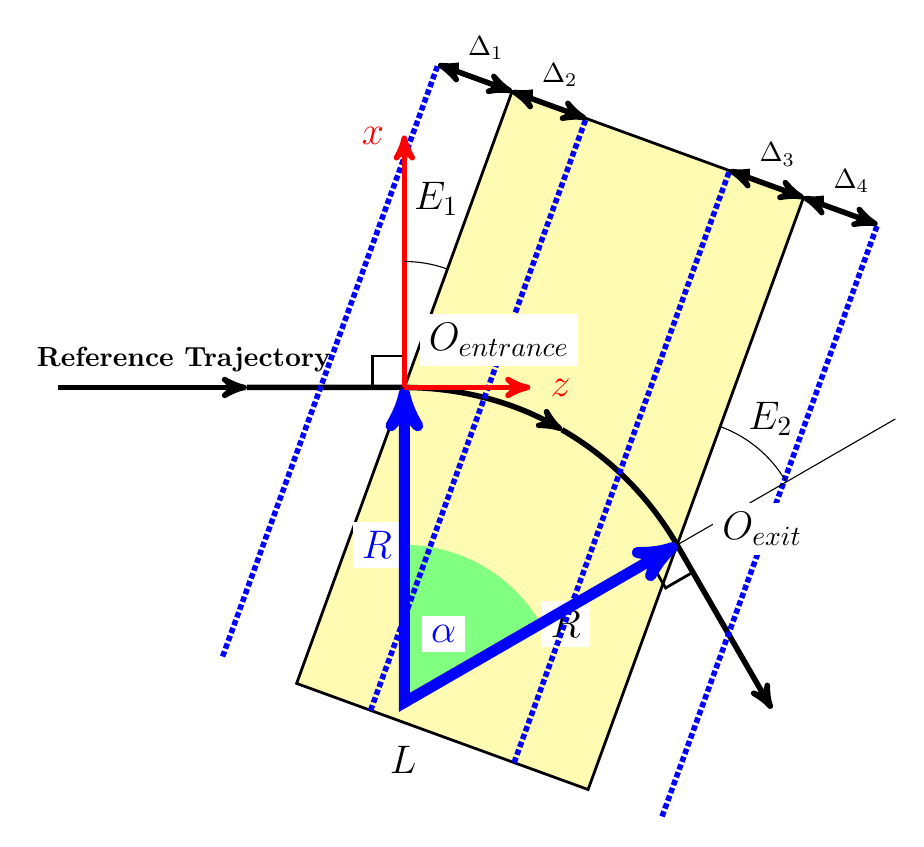
\begin{tikzpicture}[scale=4]
    \pgfmathsetmacro\Alpha{60}
    \pgfmathsetmacro\E2{40}
    \pgfmathsetmacro\sinAlpha{sin(\Alpha)}
    \pgfmathsetmacro\cosAlpha{cos(\Alpha)}
    \pgfmathsetmacro\sinAlphaHalf{sin(0.5*\Alpha)}
    \pgfmathsetmacro\cosAlphaHalf{cos(0.5*\Alpha)}
    \pgfmathsetmacro\width{2*\sinAlphaHalf*cos(10)}
    \pgfmathsetmacro\sinE2Half{sin(0.5*\E2)}
    \pgfmathsetmacro\cosE2Half{cos(0.5*\E2)}

      % First draw rectangular magnet shape.
      \begin{scope}[rotate=-20]
        \node[above=2pt] at (0.433012701892,-1.2) {\Large{\textbf{\color{black}$L$}}};
        \draw[line width=1pt,fill=yellow!30!white] (0,-1.0) rectangle (\width,1.0);
      \end{scope}

      % Now draw squares indicating 90 degree angles to bend radius at entrance and exit.
      \draw[line width=1pt] (0.0,0.0) rectangle (-0.1,0.1);
      \draw[line width=1pt,rotate around={-\Alpha:(0.0,-1.0)}]
      (0.0,-0.1) rectangle (0.1,0.0);

      % Draw reference particle path.
      \node[above=2pt] at (-0.7,0.0) {\textbf{\color{black}Reference Trajectory}};
      \draw[arrows=->,line width=2pt] (-1.1,0.0) -- (-0.5,0.0);
      \draw[arrows=->,line width=2pt] (-0.5, 0.0) -- (0.0,0.0) arc (90:60:1.0);
      \draw[arrows=->,line width=2pt] ($(0.0, -1.0) + (\sinAlphaHalf, \cosAlphaHalf)$) arc (60:30:1.0) -- +(-60:0.6);%1.1160254,-0.9330127);

      % Draw bend angle.
      \fill[green!50!white] (0.0,-1.0) -- (0.0,-0.5) arc (90:30:0.5) -- (0.0,-1.0);
      \node[fill=white] at ($(0.0,-1.0) + 0.25*(\sinAlphaHalf,\cosAlphaHalf)$) {\Large{\textbf{\color{blue}$\alpha$}}};

      \node[blue,left=1pt,fill=white] at (0.0, -0.5) {\Large{\textbf{$R$}}};
      \node[below=6pt,right=0pt,fill=white] at ($(0,-1) + 0.5*(\sinAlpha,\cosAlpha)$) {\Large{\textbf{$R$}}};
      \draw[arrows=<->,blue,line width=4pt]  (0,0) -- (0.0,-1.0) -- ($(0,-1) + (\sinAlpha, \cosAlpha)$);

      \begin{scope}[rotate=-20]
        % Draw entrance fringe field region.
        \draw[blue, densely dotted, line width=2pt] (-0.25, -1.0) -- (-0.25, 1.0);
        \draw[blue, densely dotted, line width=2pt] (0.25, -1.0) -- (0.25, 1.0);
        \draw[arrows=<->, line width=2pt] (-0.25, 1.0) -- (0.0, 1.0);
        \draw[arrows=<->, line width=2pt] (0.25, 1.0) -- (0.0, 1.0);
        \filldraw[white] (-0.125, 1.1) circle (0.1pt)
        node[fill=white] {\textbf{\color{black}$\Delta_{1}$}};
        \filldraw[white] (0.125, 1.1) circle (0.1pt)
        node[fill=white] {\textbf{\color{black}$\Delta_{2}$}};

        % Draw exit fringe field region.
        \draw[blue, densely dotted, line width=2pt] ($(\width, -1.0) - (0.25,0)$) -- ($(\width, 1.0) - (0.25,0)$);
        \draw[blue, densely dotted, line width=2pt] ($(\width, -1.0) + (0.25,0)$) -- ($(\width, 1.0) + (0.25,0)$);
        \draw[arrows=<->, line width=2pt] ($(\width, 1.0) - (0.25,0)$) -- (\width, 1.0);
        \draw[arrows=<->, line width=2pt] (\width, 1.0) -- ($(\width, 1.0) + (0.25,0)$);
        \node[fill=white] at ($(\width, 1.1) - (0.125,0)$) {\textbf{\color{black}$\Delta_{3}$}};
        \node[fill=white] at ($(\width, 1.1) + (0.125,0)$) {\textbf{\color{black}$\Delta_{4}$}};
      \end{scope}

      % Draw reference axes.
      \draw[red,arrows=->,line width=2pt] (0.0,0.0) -- (0.0,0.8) node[fill=white,left=3pt] {\Large{\textbf{$x$}}};
      \draw[red,arrows=->,line width=2pt] (0.0,0.0) -- (0.4,0.0) node[right=3pt] {\Large{\textbf{$z$}}};

      \draw (0.0, 0.4) arc (90:70:0.4);
      \node[anchor=west] at (0.0, 0.6) {\Large{$E_1$}};
      \draw ($(0,-1) + (\sinAlpha,\cosAlpha)$) -- ($(0,-1) + 1.8*(\sinAlpha,\cosAlpha)$);
      \draw ($(0,-1) + 1.4*(\sinAlpha,\cosAlpha)$) arc (30:70:0.4);
      \node at ($(1.4*\sinAlpha,-1+1.4*\cosAlpha) + (-0.05,0.2)$) {\Large{$E_2$}};

	% Label reference trajector entry and exit points.
   	\node[fill=white] at (0.3, 0.15) {\Large{$O_{entrance}$}};
	\node[fill=white, below=12pt, right=3pt] at ($(0,-1) + 1.1*(\sinAlpha,\cosAlpha)$) {\Large{\textbf{$O_{exit}$}}};
    \end{tikzpicture}
  \end{center}
  \caption{Illustration of a rectangular bend (\keyword{RBEND}, see \ssecref{RBend}) showing the entrance and exit fringe field regions. $\Delta_{1}$ is the perpendicular distance in front of the entrance edge of the magnet where the magnet fringe fields are non-negligible. $\Delta_{2}$ is the perpendicular distance behind the entrance edge of the magnet where the entrance Enge function stops being used to calculate the magnet field. The reference trajectory entrance point is indicated by $O_{entrance}$. $\Delta_{3}$ is the perpendicular distance in front of the exit edge of the magnet where the exit Enge function starts being used to calculate the magnet field. (In the region between $\Delta_{2}$ and $\Delta_{3}$ the field of the magnet is a constant value.) $\Delta_{4}$ is the perpendicular distance after the exit edge of the magnet where the magnet fringe fields are non-negligible. The reference trajectory exit point is indicated by $O_{exit}$}
  \label{fig:rbendengetype1}
\end{figure}

\begin{figure}[ht]
  \begin{center}
    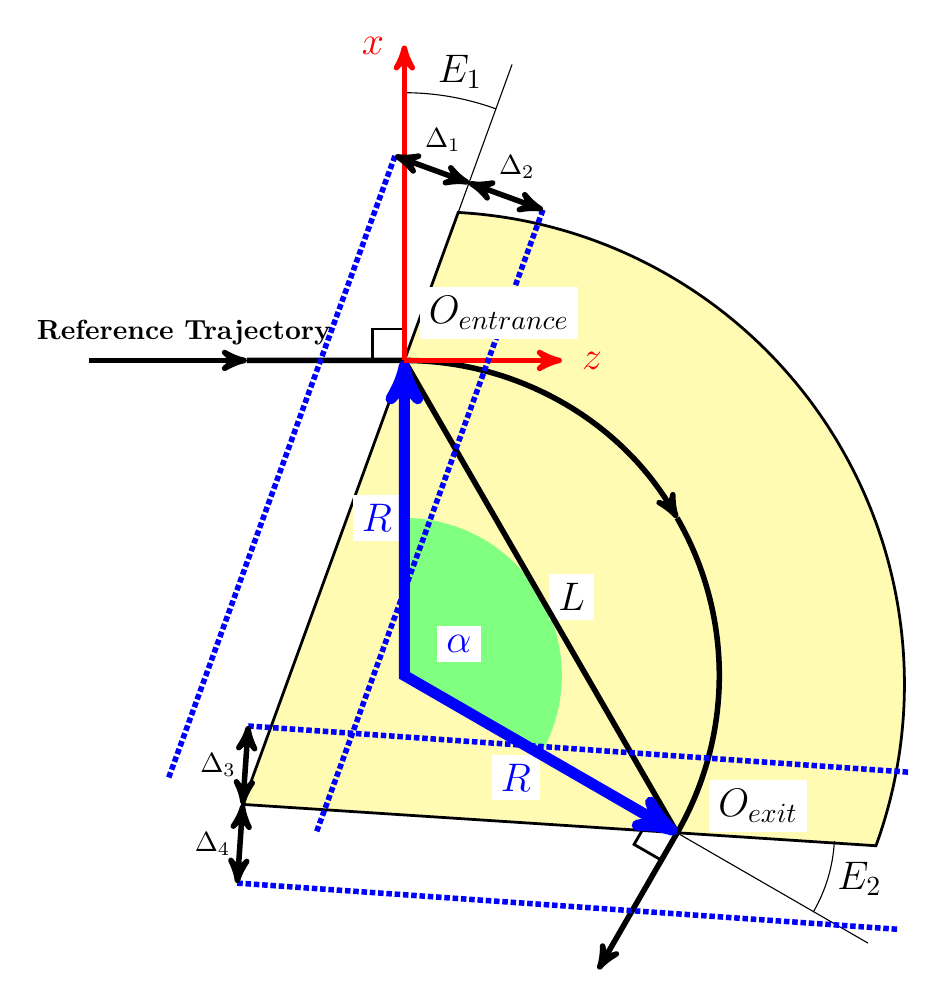
\begin{tikzpicture}[scale=4]
      % Draw magnet shape.
      \begin{scope}[rotate=-20]
        \draw[line width=1pt,fill=yellow!30!white] (0.0,-1.5)
        -- ((0.0,0.5) arc (106.82:0:1.5) -- cycle;
        \draw (0,0.5) -- (0,1);
        \draw (0,0.85) arc (90:98:0.85) node[anchor=south] {\Large{$E_1$}} arc(98:110:0.85);
      \end{scope}

      % Now draw squares indicating 90 degree angles to bend radius at entrance and exit.
      \draw[line width=1pt] (0.0,0.0) rectangle (-0.1,0.1);
      \draw[line width=1pt,xshift=0.8660254cm,yshift=-1.5cm,rotate around={60:(0.0,0.0)}]
      (-0.1,0.0) rectangle (0.0,0.1);

      % Draw reference particle path.
      \node[above=2pt] at (-0.7,0.0) {\textbf{\color{black}Reference Trajectory}};
      \draw[arrows=->,line width=2pt] (-1.,0.0) -- (-0.5,0.0);
      \draw[arrows=->,line width=2pt] (-0.5,0.0) -- (0.0,0.0) arc (90:30:1.0);
      \draw[arrows=->,line width=2pt] (0.8660254,-0.5) arc (30:-30:1.0)-- (0.6160254,-1.9330127);

      % Draw bend angle.
      \fill[green!50!white] (0.0,-1.0) -- (0.0,-0.5) arc (90:-30:0.5) -- (0.0,-1.0);
      \draw[green!50!white] (0.0,-0.8) arc (90:30:0.2)
      node[fill=white] {\Large{\textbf{\color{blue}$\alpha$}}};

      % Label chord length.
      \draw[line width=2pt] (0.0,0.0) -- (0.4330127,-0.75)
      node[fill=white,right=2pt] {\Large{\textbf{\color{black}$L$}}};
      \draw[line width=2pt] (0.4330127,-0.75) -- (0.8660254,-1.5);

      \node[blue,left=1pt,fill=white] at (0.0, -0.5) {\Large{\textbf{$R$}}};

      \node[blue,anchor=north east,fill=white] at (0.4330217,-1.25) {\Large{\textbf{$R$}}};
      \draw[arrows=<->,blue,line width=4pt] (0,0) -- (0,-1) -- (0.8660254,-1.5);
      \draw (0.8660254,-1.5) -- ($(1.7*0.8660254,-1-1.7*0.5)$);
      \draw ($(1.5*0.8660254,-1-1.5*0.5)$) arc (-30:-17:0.5) node[anchor=west] {\Large{$E_2$}} arc (-17:-3:0.5);
     % Draw reference axes.
      \draw[red,arrows=->,line width=2pt] (0.0,0.0) -- (0.0,1.0) node[left=3pt] {\Large{\textbf{$x$}}};
      \draw[red,arrows=->,line width=2pt] (0.0,0.0) -- (0.5,0.0) node[right=3pt] {\Large{\textbf{$z$}}};

      % Draw entrance fringe field region.
      \begin{scope}[rotate=-20]
        \draw[blue, densely dotted, line width=2pt] (-0.25, -1.5) -- (-0.25, 0.6);
        \draw[blue, densely dotted, line width=2pt] (0.25, -1.5) -- (0.25, 0.6);
        \draw[arrows=<->, line width=2pt] (-0.25, 0.6) -- (0.0, 0.6);
        \draw[arrows=<->, line width=2pt] (0.25, 0.6) -- (0.0, 0.6);
        \filldraw[white] (-0.125, 0.7) circle (0.1pt)
        node {\textbf{\color{black}$\Delta_{1}$}};
        \filldraw[white] (0.125, 0.7) circle (0.1pt)
        node {\textbf{\color{black}$\Delta_{2}$}};
      \end{scope}

      % Draw exit fringe field region.
      \begin{scope}[rotate around={-94:(-0.513,-1.410)}]
        \draw[blue, densely dotted, line width=2pt] (-0.763,-1.410) -- (-0.763,0.690);
        \draw[blue, densely dotted, line width=2pt] (-0.263,-1.410) -- (-0.263,0.690);
        \draw[arrows=<->,line width=2pt] (-0.763,-1.410) -- (-0.513,0.-1.410);
        \draw[arrows=<->,line width=2pt] (-0.263,-1.410) -- (-0.513,-1.410);
        \node[anchor=east] at (-0.638,-1.410) {\textbf{$\Delta_{3}$}};
        \node[anchor=east] at (-0.388,-1.410) {\textbf{$\Delta_{4}$}};
      \end{scope}

	% Label reference trajector entry and exit points.
   	\node[fill=white] at (0.3, 0.15) {\Large{$O_{entrance}$}};
   	\node[anchor=north east,fill=white] at (1.28,-1.33) {\Large{\textbf{$O_{exit}$}}};

    \end{tikzpicture}
  \end{center}
  \caption{Illustration of a sector bend (\keyword{SBEND}, see \ssecref{SBend}) showing the entrance and exit fringe field regions. $\Delta_{1}$ is the perpendicular distance in front of the entrance edge of the magnet where the magnet fringe fields are non-negligible. $\Delta_{2}$ is the perpendicular distance behind the entrance edge of the magnet where the entrance Enge function stops being used to calculate the magnet field. The reference trajectory entrance point is indicated by $O_{entrance}$. $\Delta_{3}$ is the perpendicular distance in front of the exit edge of the magnet where the exit Enge function starts being used to calculate the magnet field. (In the region between $\Delta_{2}$ and $\Delta_{3}$ the field of the magnet is a constant value.) $\Delta_{4}$ is the perpendicular distance after the exit edge of the magnet where the magnet fringe fields are non-negligible. The reference trajectory exit point is indicated by $O_{exit}$.}
  \label{fig:sbendengetype1}
\end{figure}

%\clearpage

\subsection{1DProfile1 Type 1 for Bend Magnet}
\label{ssec:1DProfile1Type1}
A \texttt{1DProfile1 Type 1} field map is the same \texttt{1DProfile1} field map found in versions of \opal previous to
\opal \opalversion{1.2.0} . \figref{rbendengetype1,sbendengetype1} illustrate the fringe field
regions for an \keyword{RBEND} and an \keyword{SBEND} element. Referring to the general field map file shown in
\tabref{1DProfile1}, the values on lines 2 and 3 are given by:

\begin{align*}
  Entrance\,Parameter\,1 &= Entrance\,Parameter\,2 - \Delta_{1} \\
  Entrance\,Parameter\,3 &= Entrance\,Parameter\,2 + \Delta_{2} \\
  Exit\,Parameter\,2 &= L - Entrance\,Parameter\,2 \\
  Exit\,Parameter\,1 &= Exit\,Parameter\,2 - \Delta_{3} \\
  Exit\,Parameter\,3 &= Exit\,Parameter\,2 + \Delta_{4}
\end{align*}
The value of $Entrance\,Parameter\,2$ can be any value. \opal only cares about the relative differences between
parameters. Also note that, internally, the origins of the entrance and exit Enge functions correspond to the
reference trajectory entrance and exit points \seefig{rbendengetype1,sbendengetype1}.

Internally, \opal reads in a \texttt{1DProfile Type 1} map and uses the provided parameters to calculate the values of:

\begin{align*}
L &= Exit\,Parameter\,2 - Entrance\,Parameter\,2 \\
\Delta_{1} &= Entrance\,Parameter\,2 - Entrance\,Parameter\,1 \\
\Delta_{2} &= Entrance\,Parameter\,3 - Entrance\,Parameter\,2 \\
\Delta_{3} &= Exit\,Parameter\,2 - Exit\,Parameter\,1 \\
\Delta_{4} &= Exit\,Parameter\,3 - Exit\,Parameter\,2
\end{align*}
These values, combined with the entrance fringe field Enge coefficients $c_0$ through $c_{N_{Enge_Entrance}}$ and exit fringe field Enge coefficients $c_0$ through $c_{N_{Enge_Exit}}$, allow \opal to find field values anywhere within the magnet. (Again, note that a \texttt{1DProfile Type 1} map always places the entrance Enge function origin at the entrance point of the reference trajectory and the exit Enge function origin at the exit point of the reference trajectory.)

\figref{1DProfile1Type1} shows an example of a \texttt{1DProfile1 Type 1} field map file.

\begin{figure}[ht]
  \begin{fmpage}
\begin{verbatim}
1DProfile1 6 7 3.0
-6.0 -2.0 2.0  1000
24.0 28.0 32.0 0
  0.00000e+00
  4.36222e-06
  8.83270e-06
  + 9 lines
  1.32490e-05
  1.73710e-05
  2.18598e-05
\end{verbatim}
  \end{fmpage}
  \caption[Example of a 1DProfile1 Type 1 field map]{A 1D field map describing the fringe field of an element using
    7 Enge coefficients for the entrance fringe field and 8 Enge coefficients for the exit fringe field (polynomial
    order 6 and 7 respectively). The element has a gap height of \SI{3.0}{\centi\meter}, and a length of \SI{30.0}{\centi\meter}. The entrance
    fringe field is non-negligible from \SI{4.0}{\centi\meter} in front of the magnet's entrance edge and reaches the core strength
    at \SI{4.0}{\centi\meter} behind the entrance edge of the magnet. (The entrance edge position is given by the element's
    \keyword{ELEMEDGE} attribute.) The exit fringe field region begins \SI{4.0}{\centi\meter} in front of the exit edge of the magnet and is non-negligible \SI{4.0}{\centi\meter} after the exit edge of the magnet. The value 1000 at the end of line 2 and 0 at the end of line 3 do not have any meaning.}
  \label{fig:1DProfile1Type1}
\end{figure}

%\clearpage

\subsection{1DProfile1 Type 2 for Bend Magnet}
\label{ssec:1DProfile1Type2}
The \texttt{1DProfile1 Type 2} field map file format was introduce in \opal \opalversion{1.2.0} to allow for more flexibility
when defining the Enge functions for the entrance and exit fringe fields. Specifically, a \texttt{1DProfile1 Type 2} map
does not contain any information about the length of the magnet. Instead, that value is set using the element's
\keyword{L} attribute. In turn, this allows us the freedom to make slight changes to how the parameters on lines 2
and 3 of the field map file shown in \tabref{1DProfile1} are defined. Now

\begin{align*}
  Entrance\,Parameter\,2 &= \perp \text{distance of entrance Enge function origin from magnet entrance edge} \\
  Exit\,Parameter\,2 &= \perp \text{distance of exit Enge function origin from magnet exit edge}
\end{align*}
The other parameters are defined the same as before:

\begin{align*}
  Entrance\,Parameter\,1 &= Entrance\,Parameter\,2 - \Delta_{1} \\
  Entrance\,Parameter\,3 &= Entrance\,Parameter\,2 + \Delta_{2} \\
  Exit\,Parameter\,1 &= Exit\,Parameter\,2 - \Delta_{3} \\
  Exit\,Parameter\,3 &= Exit\,Parameter\,2 + \Delta_{4}
\end{align*}

As before, internally, \opal reads in a \texttt{1DProfile Type 2} map and uses the provided parameters to calculate the values of:
\begin{align*}
\Delta_{1} &= Entrance\,Parameter\,2 - Entrance\,Parameter\,1 \\
\Delta_{2} &= Entrance\,Parameter\,3 - Entrance\,Parameter\,2 \\
\Delta_{3} &= Exit\,Parameter\,2 - Exit\,Parameter\,1 \\
\Delta_{4} &= Exit\,Parameter\,3 - Exit\,Parameter\,2
\end{align*}
These values, combined with the length of the magnet, \keyword{L} ( set by the element attribute) and the entrance fringe field Enge coefficients $c_0$ through $c_{N_{Enge_Entrance}}$ and exit fringe field Enge coefficients $c_0$ through $c_{N_{Enge_Exit}}$, allow \opal to find field values anywhere within the magnet.

The \texttt{1DProfile1 Type 2} field map file format has two main advantages:

\begin{enumerate}
\item The Enge function origins can be adjusted to more accurately model a magnet's fringe fields as they are no longer fixed to the entrance and exit points of the reference trajectory.
\item Two magnets with the same fringe fields, but different lengths, can be modeled with a single
  \texttt{1DProfile Type 2} field map file rather than two separate files.
\end{enumerate}
\figref{1DProfile1Type2} shows an example of a \texttt{1DProfile1 Type 2} field map file.

\begin{figure}[h]
  \begin{fmpage}
\begin{verbatim}
1DProfile1 6 7 3.0
-6.0 -2.0 2.0 0
-2.0  2.0 6.0 0
  0.00000e+00
  4.36222e-06
  8.83270e-06
  + 9 lines
  1.32490e-05
  1.73710e-05
  2.18598e-05
\end{verbatim}
\end{fmpage}
\caption[Example of a 1DProfile1 Type 2 field map]{A 1D field map describing the fringe field of an element using 7 Enge coefficients for the entrance fringe field and 8 Enge coefficients for the exit fringe field (polynomial order 6 and 7 respectively). The element has a gap height of \SI{3.0}{\centi\meter}. The entrance fringe field is non-negligible from \SI{4.0}{\centi\meter} in front of the magnet's entrance edge and reaches the core strength at \SI{4.0}{\centi\meter} behind the entrance edge of the magnet. The exit fringe field region begins \SI{4.0}{\centi\meter} in front of the exit edge of the magnet and is non-negligible \SI{4.0}{\centi\meter} after the exit edge of the magnet. The value 0 at the end of line 2 and 0 at the end of line 3 do not have any meaning. The entrance Enge function origin is \SI{2.0}{\centi\meter} in front (upstream) of the magnet's entrance edge. The exit Enge function origin is \SI{2.0}{\centi\meter} behind (downstream of) the exit edge of the magnet.}
\label{fig:1DProfile1Type2}
\end{figure}

%\clearpage


\section{2DElectroStatic}
\label{sec:2DElectroStatic}
\index{2DElectroStatic}
\index{Field Map!2DElectroStatic}
\begin{figure}[h]
  \begin{fmpage}
\begin{verbatim}
2DElectroStatic XZ
-3.0 51.0 4999
0.0 2.0 199
  0.00000e+00  0.00000e+00
  4.36222e-06  0.00000e+00
  8.83270e-06  0.00000e+00
  + 999994 lines
  1.32490e-05  0.00000e+00
  1.73710e-05  0.00000e+00
  2.18598e-05  0.00000e+00
\end{verbatim}
  \end{fmpage}
  \caption[Example of a 2DElectroStatic field map]{A 2D field map describing an electrostatic field using 5000 grid points
    in the longitudinal direction times 200 grid points in the radial direction. The field between the grid points is calculated
    using bi-linear interpolation. The field is non-negligible from \SI{-3.0}{\centi\meter} to \SI{51.0}{\centi\meter} relative to \keyword{ELEMEDGE} and the 200
    grid points in the radial direction span the distance from \SI{0.0}{\centi\meter} to \SI{2.0}{\centi\meter}. The field values are ordered in XZ
    orientation, so the index in the longitudinal direction changes fastest and therefore $E_z$ values are stored in the first
    column and $E_r$ values in the second \seesec{fieldorientation}. \opalt normalizes the field so that $max(|E_{z, \text{ on axis}}|) = \SI{1}{\mega\volt\per\meter}$.}
  \label{fig:2DElectroStatic}
\end{figure}

\begin{table}[ht!]
    \caption{Layout of a \texttt{2DElectroStatic} field map file.}
    \label{tab:2DElectroStatic}
    \begin{center}
    \begin{tabular}{lll}
      \hline
      2DElectroStatic & Orientation (XZ or ZX) & \\
      $z_{start}$ (or $r_{start}$) (in cm) & $z_{end}$ (or $r_{end}$) (in cm) & $N_{z}$ (or $N_{r}$) \\
      $r_{start}$ (or $z_{start}$) (in cm) & $r_{end}$ (or $z_{end}$) (in cm) & $N_{r}$ (or $N_{z}$) \\
      $E_{z,\,1}$ (or $E_{r,\,1}$) (MV/m) & $E_{r,\,1}$ (or $E_{z,\,1}$) (MV/m)& \\
      $E_{z,\,2}$ (or $E_{r,\,2}$) (MV/m) & $E_{r,\,2}$ (or $E_{z,\,2}$) (MV/m)& \\
      . & & \\
      . & & \\
      . & & \\
      $E_{z,\,N}$ (or $E_{r,\,N}$) (MV/m) & $E_{r,\,N}$ (or $E_{z,\,N}$) (MV/m)& \\
      \hline
    \end{tabular}
    \end{center}
\end{table}

A \texttt{2DElectroStatic} field map has the general form shown in \tabref{2DElectroStatic}. The first three lines form
the file header and tell \opalt how the field map data is being presented:

\begin{description}
\item[Line 1] This tells \opalt what type of field file it is (\texttt{2DElectroStatic}) and the field orientation
  \seesec{fieldorientation}.
\item[Line 2] This gives the extent of the field map and how many grid spacings there are in the fastest changing
  index direction \seesec{fieldorientation}.
\item[Line 3] This gives the extent of the field map and how many grid spacings there are in the slowest changing
  index direction (see \secref{fieldorientation}.
\end{description}

The lines following the header give the 2D field map grid values from $1$ to $N = (N_{z} + 1) \times (N_{r} + 1)$.
The order of these depend on the field orientation \seesec{fieldorientation} and can be one of two formats:

\begin{description}
\item[If Orientation = XZ:] $E_{z}$ (MV/m) $E_{r}$ (MV/m)
\item[If Orientation = ZX:] $E_{r}$ (MV/m) $E_{z}$ (MV/m)
\end{description}

\figref{2DElectroStatic} gives an example of a \texttt{2DElectroStatic} field file.

%\clearpage

\section{2DMagnetoStatic}
\label{sec:2DMagnetoStatic}
\index{2DMagnetoStatic}
\index{Field Map!2DMagnetoStatic}
\begin{figure}[h]
  \begin{fmpage}
\begin{verbatim}
2DMagnetoStatic ZX
0.0 2.0 199
-3.0 51.0 4999
  0.00000e+00  0.00000e+00
  0.00000e+00  4.36222e-06
  0.00000e+00  8.83270e-06
  + 999994 lines
  0.00000e+00  1.32490e-05
  0.00000e+00  1.73710e-05
  0.00000e+00  2.18598e-05
\end{verbatim}
  \end{fmpage}
  \caption[Example of a 2DMagnetoStatic field map]{A 2D field map describing a magnetostatic field using 5000 grid points
    in the longitudinal direction times 200 grid points in the radial direction. The field between the grid points is calculated
    using bi-linear interpolation. The field is non-negligible from \SI{-3.0}{\centi\meter} to \SI{51.0}{\centi\meter} relative to \keyword{ELEMEDGE} and the 200 grid
    points in the radial direction span the distance from \SI{0.0}{\centi\meter} to \SI{2.0}{\centi\meter}. The field values are ordered in the ZX
    orientation, so the index in the radial direction changes fastest and therefore $B_r$ values are stored in the first column
    and $B_z$ values in the second \seesec{fieldorientation}. \opalt normalizes the field so that $max(|B_{z,\text{ on axis}}|) = \SI{1}{\tesla}$.}
  \label{fig:2DMagnetoStatic}
\end{figure}

\begin{table}[ht!]
    \caption{Layout of a \texttt{2DMagnetoStatic} field map file.}
    \label{tab:2DMagnetoStatic}
    \begin{center}
    \begin{tabular}{lll}
      \hline
      2DMagnetoStatic & Orientation (XZ or ZX) & \\
      $z_{start}$ (or $r_{start}$) (in cm) & $z_{end}$ (or $r_{end}$) (in cm) & $N_{z}$ (or $N_{r}$) \\
      $r_{start}$ (or $z_{start}$) (in cm) & $r_{end}$ (or $z_{end}$) (in cm) & $N_{r}$ (or $N_{z}$) \\
      $B_{z,\,1}$ (or $B_{r,\,1}$) (T) & $B_{r,\,1}$ (or $B_{z,\,1}$) (T)& \\
      $B_{z,\,2}$ (or $B_{r,\,2}$) (T) & $B_{r,\,2}$ (or $B_{z,\,2}$) (T)& \\
      . & & \\
      . & & \\
      . & & \\
      $B_{z,\,N}$ (or $B_{r,\,N}$) (T) & $B_{r,\,N}$ (or $B_{z,\,N}$) (T)& \\
      \hline
    \end{tabular}
    \end{center}
\end{table}

A \texttt{2MagnetoStatic} field map has the general form shown in \tabref{2DMagnetoStatic}. The first three lines form
the file header and tell \opalt how the field map data is being presented:

\begin{description}
\item[Line 1] This tells \opalt what type of field file it is (\texttt{2DMagnetoStatic}) and the field orientation
  \seesec{fieldorientation}.
\item[Line 2] This gives the extent of the field map and how many grid spacings there are in the fastest changing
  index direction \seesec{fieldorientation}.
\item[Line 3] This gives the extent of the field map and how many grid spacings there are in the slowest changing
  index direction (see \secref{fieldorientation}.
\end{description}

The lines following the header give the 2D field map grid values from $1$ to $N = (N_{z} + 1) \times (N_{r} + 1)$.
The order of these depend on the field orientation \seesec{fieldorientation} and can be one of two formats:

\begin{description}
\item[If Orientation = XZ:] $B_{z}$ (T) $B_{r}$ (T)
\item[If Orientation = ZX:] $B_{r}$ (T)  $B_{z}$ (T)
\end{description}

\figref{2DMagnetoStatic} gives an example of a \texttt{2DMagnetoStatic} field file.

%\clearpage

\section{2DDynamic}
\label{sec:2DDynamic}
\index{2DDynamic}
\index{Field Map!2DDynamic}
\begin{figure}[h]
  \begin{fmpage}
\begin{verbatim}
2DDynamic XZ
-3.0 51.0 4121
1498.953425154
0.0 1.0 75
  0.00000e+00  0.00000e+00  0.00000e+00  0.00000e+00
  4.36222e-06  0.00000e+00  0.00000e+00  4.36222e-06
  8.83270e-06  0.00000e+00  0.00000e+00  8.83270e-06
  + 313266 lines
  1.32490e-05  0.00000e+00  0.00000e+00  1.32490e-05
  1.73710e-05  0.00000e+00  0.00000e+00  1.73710e-05
  2.18598e-05  0.00000e+00  0.00000e+00  2.18598e-05
\end{verbatim}
  \end{fmpage}
  \caption[Example of a 2DDynamic field map]{A 2D field map describing a dynamic field oscillating with a frequency of
    \SI{1498.953425154}{\mega\hertz}. The field map provides 4122 grid points in the longitudinal direction times 76 grid points in
    radial direction. The field between the grid points is calculated with a bi-linear interpolation. The field is
    non-negligible between \SI{-3.0}{\centi\meter} and \SI{51.0}{\centi\meter} relative to \keyword{ELEMEDGE} and the 76 grid points in radial direction
    span the distance from \SI{0.0}{\centi\meter} to \SI{1.0}{\centi\meter}. The field values are ordered in the XZ orientation, so the index in the
    longitudinal direction changes fastest and therefore $E_z$ values are stored in the first column and $E_r$ values
    in the second. The third column contains the electric field magnitude, $|E|$, and is not used (but must still be included).
    The fourth column is $H_{\phi}$ in A/m. The third and fourth columns are always the same and do not depend on the field
    orientation \seesec{fieldorientation}. \opalt normalizes the field so that $max(|E_{z,\text{ on axis}}|) = \SI{1}{\mega\volt\per\meter}$.}
  \label{fig:2DDynamic}
\end{figure}

\begin{table}[ht!]
    \caption{Layout of a \texttt{2DDynamic} field map file.}
    \label{tab:2DDynamic}
    \begin{center}
    \begin{tabular}{llll}
      \hline
      2DDynamic & Orientation (XZ or ZX) & & \\
      $z_{start}$ (or $r_{start}$) (in cm) & $z_{end}$ (or $r_{end}$) (in cm) & $N_{z}$ (or $N_{r}$)& \\
      $Frequency$ (in MHz) & & & \\
      $r_{start}$ (or $z_{start}$) (in cm) & $r_{end}$ (or $z_{end}$) (in cm) & $N_{r}$ (or $N_{z}$)& \\
      $E_{z,\,1}$ (or $E_{r,\,1}$) (MV/m)) & $E_{r,\,1}$ (or $E_{z,\,1}$) (MV/m) & $|E_1|$ (MV/m) & $H_{\phi,\,1}$ (A/m) \\
      $E_{z,\,2}$ (or $E_{r,\,2}$) (MV/m)) & $E_{r,\,2}$ (or $E_{z,\,2}$) (MV/m) & $|E_2|$ (MV/m) & $H_{\phi,\,2}$ (A/m) \\
      . & & \\
      . & & \\
      . & & \\
      $E_{z,\,N}$ (or $E_{r,\,N}$) (MV/m)) & $E_{r,\,N}$ (or $E_{z,\,N}$) (MV/m) & $|E_N|$ (MV/m) & $H_{\phi,\,N}$ (A/m) \\
      \hline
    \end{tabular}
    \end{center}
\end{table}

A \texttt{2DDynamic} field map has the general form shown in \tabref{2DDynamic}. The first four lines form
the file header and tell \opalt how the field map data is being presented:

\begin{description}
\item[Line 1] This tells \opalt what type of field file it is (\texttt{2DDynamic}) and the field orientation
  \seesec{fieldorientation}.
\item[Line 2] This gives the extent of the field map and how many grid spacings there are in the fastest changing
  index direction \seesec{fieldorientation}.
\item[Line 3] Field frequency.
\item[Line 4] This gives the extent of the field map and how many grid spacings there are in the slowest changing
  index direction \seesec{fieldorientation}.
\end{description}

The lines following the header give the 2D field map grid values from $1$ to $N= (N_{z} + 1) \times (N_{r} + 1)$. The
order of these depend on the field orientation \seesec{fieldorientation} and can be one of two formats:
\begin{description}
\item[If Orientation = XZ:] $E_{z}$ (MV/m) $E_{r}$ (MV/m) $|E|$ (MV/m) $H_{\phi}$ (A/m)
\item[If Orientation = ZX:] $E_{r}$ (MV/m) $E_{z}$ (MV/m) $|E|$ (MV/m) $H_{\phi}$ (A/m)
\end{description}
The third item (the field magnitude) on each data line is not used by \opalt, but must be there.

\figref{2DDynamic} gives an example of a \texttt{2DDynamic} field file.
%\clearpage
\section{3DMagnetoStatic}
\label{sec:3DMagnetoStatic}
\index{3DMagnetoStatic}
\index{Field Map!3DMagnetoStatic}
\begin{figure}[h]
  \begin{fmpage}
\begin{verbatim}
3DMagnetoStatic
-1.5 1.5 227
-1.0 1.0 151
-3.0 51.0 4121
0.00e+00 0.00e+00 0.00e+00
0.00e+00 4.36e-06 0.00e+00
0.00e+00 8.83e-06 0.00e+00
+ 142'852'026 lines
0.00e+00 1.32e-05 0.00e+00
0.00e+00 1.73e-05 0.00e+00
0.00e+00 2.18e-05 0.00e+00
\end{verbatim}
  \end{fmpage}
  \caption[Example of a 3DMagnetoStatic field map]{A 3D field map describing a magnetostatic field.
    The field map provides 4122 grid points in z-direction times 228 grid points in x-direction and 152 grid points in y-direction.
    The field between the grid points is calculated with a tri-linear interpolation. The field is non-negligible between \SI{-3.0}{\centi\meter}
    to \SI{51.0}{\centi\meter} relative to \keyword{ELEMEDGE}, the 228 grid points in x-direction range from \SI{-1.5}{\centi\meter} to \SI{1.5}{\centi\meter} and the 152 grid
    points in y-direction range from \SI{-1.0}{\centi\meter} to \SI{1.0}{\centi\meter} relative to the design path. The field values are ordered such that the index in z-direction changes fastest, then the index in y-direction while the index in x-direction changes
    slowest. The columns correspond to $B_x$, $B_y$ and $B_z$.}
  \label{fig:3DMagnetoStatic}
\end{figure}

\begin{table}[ht!]
    \caption{Layout of a \texttt{3DMagnetoStatic} field map file.}
    \label{tab:3DMagnetoStatic}
    \begin{center}
    \begin{tabular}{llllll}
      \hline
      3DMagnetoStatic     &                   &                   \\
      $x_{start}$ (in cm) & $x_{end}$ (in cm) & $N_{x}$           \\
      $y_{start}$ (in cm) & $y_{end}$ (in cm) & $N_{y}$           \\
      $z_{start}$ (in cm) & $z_{end}$ (in cm) & $N_{z}$           \\
      $B_{x,\,1}$ (A/m)   & $B_{y,\,1}$ (A/m) & $B_{z,\,1}$ (A/m) \\
      $B_{x,\,2}$ (A/m)   & $B_{y,\,2}$ (A/m) & $B_{z,\,2}$ (A/m) \\
      .                   &                   &                   \\
      .                   &                   &                   \\
      .                   &                   &                   \\
      $B_{x,\,N}$ (A/m)   & $B_{y,\,N}$ (A/m) & $B_{z,\,N}$ (A/m) \\
      \hline
    \end{tabular}
    \end{center}
\end{table}

A \texttt{3DMagnetoStatic} field map has the general form shown in \tabref{3DMagnetoStatic}. The first five lines form
the file header and tell \opalt how the field map data is being presented:

\begin{description}
\item[Line 1] This tells \opalt what type of field file it is (\texttt{3DMagnetoStatic}).
\item[Line 3] This gives the extent of the field map and how many grid spacings there are in the slowest changing
  index direction.
\item[Line 4] This gives the extent of the field map and how many grid spacings there are in the next fastest changing
  index direction.
\item[Line 5] This gives the extent of the field map and how many grid spacings there are in the fastest changing
  index direction.
\end{description}

The lines following the header give the 3D field map grid values from $1$ to $N= (N_{z} + 1) \times (N_{y} + 1) \times (N_{x} + 1)$.
\figref{3DMagnetoStatic} gives an example of a \texttt{3DMagnetoStatic} field file.

\newpage
\section{3DMagnetoStatic\_Extended}
\label{sec:3DMagnetoStatic_Extended}
\index{3DMagnetoStatic\_Extended}
\index{Field Map!3DMagnetoStatic\_Extended}
\begin{figure}[h]
  \begin{fmpage}
\begin{verbatim}
3DMagnetoStatic_Extended
-9.9254 9.9254 133
-2.0 1.0 15
-22.425 47.425 465
 -8.10970000e-05
 -8.38540000e-05
 -8.64960000e-05
+ 62'438 lines
 -8.64960000e-05
 -8.38540000e-05
 -8.10970000e-05
\end{verbatim}
  \end{fmpage}
  \caption[Example of a 3DMagnetoStatic\_Extended field map]{A 3D field map describing a magnetostatic field on the mid-plane. The field map provides 466 grid points in z-direction times 134 grid points in x-direction. The field is non-negligible between \SI{-22.425}{\centi\meter} to \SI{47.425}{\centi\meter} relative to \keyword{ELEMEDGE}, the 134 grid points in x-direction range from \SI{-9.9254}{\centi\meter} to \SI{9.9254}{\centi\meter}. The field should be integrated using Maxwell's equations from the mid-plane to \SI{2.0}{\centi\meter} using 16 grid points. The mid-plane is regarded as a perfect magnetic conductor (PMC) i.e. the magnetic field on the mid-plane has no tangential component. This leads to a symmetry where the perpendicular component is mirrored whereas the tangential component is anti-parallel. Instead of integrating the field from the mid-plane to \SI{-2.0}{\centi\meter} and \SI{1.0}{\centi\meter} we only integrate it to \SI{+2.0}{\centi\meter} and store only the upper half of the field map. For positions $R(x,\;-y,\;z)$ with $y > 0.0$ the correct field can then be derived from the $R(x,\;y,\;z)$.}
  \label{fig:3DMagnetoStatic_Extended}
\end{figure}

\begin{table}[ht!]
    \caption{Layout of a \texttt{3DMagnetoStatic\_Extended} field map file.}
    \label{tab:3DMagnetoStatic_Extended}
    \begin{center}
    \begin{tabular}{lll}
      \hline
      \multicolumn{2}{l}{3DMagnetoStatic\_Extended}  &           \\
      $x_{start}$ (in cm)       & $x_{end}$ (in cm)  & $N_{x}$   \\
      $y_{start}$ (in cm)       & $y_{end}$ (in cm)  & $N_{y}$   \\
      $z_{start}$ (in cm)       & $z_{end}$ (in cm)  & $N_{z}$   \\
      $B_{y,\,1}$ (T)           &                    &           \\
      $B_{y,\,2}$ (T)           &                    &           \\
      .                         &                    &           \\
      .                         &                    &           \\
      .                         &                    &           \\
      $B_{y,\,N}$ (T)           &                    &           \\
      \hline
    \end{tabular}
    \end{center}
\end{table}

A \texttt{3DMagnetoStatic\_Extended} field map has the general form shown in \tabref{3DMagnetoStatic_Extended}. The first four lines form the file header and tell \opalt how the field map data is being presented:

\begin{description}
\item[Line 1] This tells \opalt what type of field file it is (\texttt{3DMagnetoStatic\_Extended}).
\item[Line 2] This gives the extent of the field map and how many grid spacings there are in the slowest changing direction.
\item[Line 3] This gives the extent of the field map and how many grid spacings there are in the next fastest changing direction.
\item[Line 4] This gives the extent of the field map and how many grid spacings there are in the fastest changing direction.
\end{description}

The lines following the header give the 3D field map grid values from $1$ to $N= (N_{z} + 1) \times (N_{x} + 1)$.
The order of these depend on the field orientation \seesec{fieldorientation} and can currently only be the
format shown in \tabref{3DMagnetoStatic_Extended}.

\figref{3DMagnetoStatic_Extended} gives an example of a \texttt{3DMagnetoStatic\_Extended} field file.

%\clearpage
\section{3DDynamic}
\label{sec:3DDynamic}
\index{3DDynamic}
\index{Field Map!3DDynamic}
\begin{figure}[h]
  \begin{fmpage}
\begin{verbatim}
3DDynamic
1498.953425154
-1.5 1.5 227
-1.0 1.0 151
-3.0 51.0 4121
0.00e+00 0.00e+00 0.00e+00 0.00e+00 0.00e+00 0.00e+00
4.36e-06 0.00e+00 4.36e-06 0.00e+00 4.36e-06 0.00e+00
8.83e-06 0.00e+00 8.83e-06 0.00e+00 8.83e-06 0.00e+00
+ 142'852'026 lines
1.32e-05 0.00e+00 1.32e-05 0.00e+00 1.32e-05 0.00e+00
1.73e-05 0.00e+00 1.73e-05 0.00e+00 1.73e-05 0.00e+00
2.18e-05 0.00e+00 2.18e-05 0.00e+00 2.18e-05 0.00e+00
\end{verbatim}
  \end{fmpage}
  \caption[Example of a 3DDynamic field map]{A 3D field map describing a dynamic field oscillating with \SI{1.498953425154}{\giga\hertz}.
    The field map provides 4122 grid points in z-direction times 228 grid points in x-direction and 152 grid points in y-direction.
    The field between the grid points is calculated with a tri-linear interpolation. The field is non-negligible between \SI{-3.0}{\centi\meter}
    to \SI{51.0}{\centi\meter} relative to \keyword{ELEMEDGE}, the 228 grid points in x-direction range from \SI{-1.5}{\centi\meter} to \SI{1.5}{\centi\meter} and the 152 grid
    points in y-direction range from \SI{-1.0}{\centi\meter} to \SI{1.0}{\centi\meter} relative to the design path. The field values are ordered such that the index in z-direction changes fastest, then the index in y-direction while the index in x-direction changes
    slowest. The columns correspond to $E_x$, $E_y$, $E_z$, $H_x$, $H_y$ and $H_z$.}
  \label{fig:3DDynamic}
\end{figure}

\begin{table}[ht!]
    \caption{Layout of a \texttt{3DDynamic} field map file.}
    \label{tab:3DDynamic}
    \begin{center}
    \begin{tabular}{llllll}
      \hline
      3DDynamic            &                    &                    &                   &                   &                   \\
      $Frequency$ (in MHz) &                    &                    &                   &                   &                   \\
      $x_{start}$ (in cm)  & $x_{end}$ (in cm)  & $N_{x}$            &                   &                   &                   \\
      $y_{start}$ (in cm)  & $y_{end}$ (in cm)  & $N_{y}$            &                   &                   &                   \\
      $z_{start}$ (in cm)  & $z_{end}$ (in cm)  & $N_{z}$            &                   &                   &                   \\
      $E_{x,\,1}$ (MV/m))  & $E_{y,\,1}$ (MV/m) & $E_{z,\,1}$ (MV/m) & $H_{x,\,1}$ (A/m) & $H_{y,\,1}$ (A/m) & $H_{z,\,1}$ (A/m) \\
      $E_{x,\,2}$ (MV/m))  & $E_{y,\,2}$ (MV/m) & $E_{z,\,2}$ (MV/m) & $H_{x,\,2}$ (A/m) & $H_{y,\,2}$ (A/m) & $H_{z,\,2}$ (A/m) \\
      .                    &                    &                    &                   &                   &                   \\
      .                    &                    &                    &                   &                   &                   \\
      .                    &                    &                    &                   &                   &                   \\
      $E_{x,\,N}$ (MV/m))  & $E_{y,\,N}$ (MV/m) & $E_{z,\,N}$ (MV/m) & $H_{x,\,N}$ (A/m) & $H_{y,\,N}$ (A/m) & $H_{z,\,N}$ (A/m) \\
      \hline
    \end{tabular}
    \end{center}
\end{table}

A \texttt{3DDynamic} field map has the general form shown in \tabref{3DDynamic}. The first five lines form
the file header and tell \opalt how the field map data is being presented:

\begin{description}
\item[Line 1] This tells \opalt what type of field file it is (\texttt{3DDynamic}).
\item[Line 2] Field frequency.
\item[Line 3] This gives the extent of the field map and how many grid spacings there are in the slowest changing
  index direction.
\item[Line 4] This gives the extent of the field map and how many grid spacings there are in the next fastest changing
  index direction.
\item[Line 5] This gives the extent of the field map and how many grid spacings there are in the fastest changing
  index direction.
\end{description}

The lines following the header give the 3D field map grid values from $1$ to $N= (N_{z} + 1) \times (N_{y} + 1) \times (N_{x} + 1)$.
\figref{3DDynamic} gives an example of a \texttt{3DDynamic} field file.

%----------- Footer control ------------------
\ifthenelse{\boolean{FullOPALManual}}
{
  %do nothing
}
% else (for individual document creation)
{
\appendix
\printbibliography
\end{document}
}
%---------------------------------------------
\ifdefined \buildingFullOPALManual \else


%\ifx \@buildingFullOPALManual \@empty
%\else

%\documentclass[12pt,a4paper]{report}
\documentclass[a4paper]{book}

%% does not work in Latex2Html mode
%\usepackage{hyperref}

\usepackage[T1]{fontenc}
\usepackage{url}
\usepackage{html}
\usepackage{epic}
\usepackage{eepic}
\usepackage{makeidx}
\usepackage{array}
\usepackage{times}
\usepackage{amsmath}
\usepackage{amsxtra}
\usepackage{bm}
\usepackage[thin,thinp,thinc]{esdiff}
\usepackage{etoolbox}
\usepackage{graphicx}
\usepackage{dingbat}
\usepackage{color}
\usepackage{subfig}
\usepackage{boxedminipage}
\usepackage{alltt}
\usepackage{nicefrac}
\usepackage{calc}
%\usepackage{pdfdraftcopy}             % Draft
\usepackage{tikz}
\usetikzlibrary{
  er,3d,calc,fadings,trees,positioning,arrows,chains,decorations.pathreplacing,
  decorations.pathmorphing,shapes,shapes.symbols,shapes.arrows,matrix,through,decorations.text
}

\tikzset{
  >=stealth',
  punktchain/.style={rectangle,rounded corners, draw=black, very thick,text width=10em,
                     minimum height=3em, text centered, on chain},
  line/.style={draw, thick, <-},
  element/.style={tape,top color=white,bottom color=blue!50!black!60!,minimum width=8em,
                  draw=blue!40!black!90, very thick,text width=10em, minimum height=3.5em,
                  text centered, on chain},
  every join/.style={->, thick,shorten >=1pt},
  tuborg/.style={decorate},
  tubnode/.style={midway, right=2pt}
}

\tikzstyle{material}=[draw, fill=blue!20, text width=16.0em, text centered, minimum height=1.5em]
\tikzstyle{diagramstep} = [material, text width=20em, minimum width=10em, minimum height=3em, rounded corners]
\tikzstyle{line} = [draw, thick, color=black!50, -latex']

\usepackage{booktabs}
\usepackage{xspace}
\usepackage{xstring}

\usepackage{fancyvrb}
\usepackage{rotating}
\usepackage{float}

\usepackage{tabularx}
\usepackage{longtable}
\setcounter{LTchunksize}{3}

\usepackage[section]{placeins}
\usepackage{MnSymbol}
\usepackage{microtype}
\usepackage{setspace}
\usepackage{dcolumn}

\usepackage[vmargin={3.0cm,3.0cm},
            hmargin={2.0cm,3.0cm}]{geometry}

\usepackage{upgreek}
\usepackage[binary-units=true]{siunitx}
\sisetup{exponent-product = \cdot,math-ohm=\Upomega,text-ohm=\ensuremath{\Upomega}}
\DeclareSIUnit{\clight}{c}
\DeclareSIUnit\gauss{Ga}

\usepackage{engord}
\usepackage{wasysym}
\DeclareSIUnit[number-unit-product = \,]{\permill}{\permil}

\usepackage{hyperref}
\hypersetup{
    pdftitle          = The OPAL Framework,
    pdfauthor         = {Andreas Adelmann, Achim Gsell, Valeria Rizzoglio, Christof Metzger-Kraus,
                         Yves Ineichen, Xiaoying Pang, Steve Russell, Chuan Wang, Jianjun Yang,
                         Suzanne Sheehy, Chris Rogers, Daniel Winklehner},
    pdfsubject        = User's Reference Manual,
    pdffitwindow      = true,               % page fit to window when opened
    pdfnewwindow      = true,               % links in new window
    colorlinks        = true,               % false: boxed links; true: colored links
    linkcolor         = black!80!green,     % color of internal links
    citecolor         = black!20!red,       % color of links to bibliography
    urlcolor          = blue,               % color of external links
    breaklinks        = true,
    bookmarksnumbered = true,
    plainpages        = false
}

\usepackage{ifthen}

\newif \iflinuxwindows
\linuxwindowstrue   % set this to true when building the manual on Linux or Windows
\iflinuxwindows
\usepackage{epstopdf}
\fi

\usepackage[backend=biber,
            style=phys,
            biblabel=brackets,
            maxnames=3,
            doi=true,
            isbn=true,
            url=true]{biblatex}
%---- macros ----

\renewcommand{\topfraction}{1.0}
\renewcommand{\bottomfraction}{1.0}
\renewcommand{\textfraction}{0.0}
\renewcommand{\arraystretch}{2.0}
\newenvironment{tex2html_nowrap}{}{}


\newcommand{\Newline}{\hfil \\}


\newsavebox{\ExampleBox}
\newenvironment{example}
 {\VerbatimEnvironment
  \begin{flushleft}
  \begin{lrbox}{\ExampleBox}
    \begin{minipage}{\linewidth}
  \begin{Verbatim}[frame=lines,xleftmargin=0cm,fontsize=\footnotesize,samepage=true]}
 {\end{Verbatim}
  \end{minipage}
  \end{lrbox}
  \mbox{\usebox{\ExampleBox}}
  \end{flushleft}
 }

\newenvironment{longexample}
{\Verbatim[frame=lines,xleftmargin=0mm,fontsize=\footnotesize]}
{\endVerbatim}

%\examplefromfile{filename} reads in a text file and displays it in the document.
\newcommand{\examplefromfile}[1]{
\VerbatimInput[frame=lines,xleftmargin=0mm,fontsize=\footnotesize,label=\texttt{#1}]{#1}}

%for upright d of differentials
\makeatletter
\newcount\my@repeat@count

\newcommand{\myrepeat}[2]{%
  \begingroup
  \my@repeat@count=\z@
  \@whilenum\my@repeat@count<#1\do{#2\advance\my@repeat@count\@ne}%
  \endgroup
}

\newcommand{\differential}[1]{\ifstrempty{#1}{\ES@dop\ES@difint}{\ES@dop^{#1}\ES@difint}}
\newcommand{\pdifferential}[1]{\ifstrempty{#1}{{\partial\,}}{{\partial^{#1}\,}}}

\makeatother

\newcommand{\der}[3][]{\frac{\differential{#1}#2}{\differential{}\ifstrempty{#1}{#3}{#3^#1}}}
\newcommand{\parder}[3][]{\frac{\pdifferential{#1}#2}{\pdifferential{}\ifstrempty{#1}{#3}{#3^#1}}}
\newcommand{\niceder}[3][]{\nicefrac{\differential{#1}#2}{\differential{}\ifstrempty{#1}{#3}{#3^#1}}}
\newcommand{\uglyder}[3][]{{\differential{#1}#2}/{\differential{}\ifstrempty{#1}{#3}{#3^#1}}}
\newcommand{\uglyparder}[3][]{{\pdifferential{#1}#2}/{\pdifferential{}\ifstrempty{#1}{#3}{#3^#1}}}
\newcommand{\dd}[1][]{\; \differential{#1}}
\newcommand{\primed}{^{\prime}}
\newcommand{\dprimed}{^{\prime\prime}}
\newcommand{\nprimed}[1]{^{\myrepeat{#1}{\prime}}}

%Editing Macros
\newcommand{\TODO}[1]{{\color{red}\ifthenelse{\boolean{ShowDebug}}{[TODO: #1]}{}}}



%text in gray box
\newsavebox{\fmbox}
\definecolor{lightgray}{gray}{0.95}
\newenvironment{fmpage}
   {\vspace{-1.0cm}\begin{lrbox}{\fmbox}\begin{minipage}[t]{13.5cm}\vspace{0.1cm}}
   {\vspace{-0.4cm}\end{minipage}\end{lrbox}\begin{center}\fcolorbox{black}{lightgray}{\usebox{\fmbox}}\end{center}}


% Definition new signes
\newcommand{\R}{{\mathbb R}} % real numbers
\newcommand{\Q}{{\mathbb Q}} % rational numbers
\newcommand{\Z}{{\mathbb Z}} % integer numbers
\newcommand{\N}{{\mathbb N}} % natural numbers

\newcommand{\mad}{\textsc{mad}\xspace}
\newcommand{\madnine}{\textsc{mad9}\xspace}
\newcommand{\madninep}{\textsc{mad9p}\xspace}
\newcommand{\madeight}{\textsc{mad8}\xspace}
\newcommand{\classic}{\textsc{classic}\xspace}

\makeatletter
\newcommand{\opal@impl}{\textsc{Opal}}
\newcommand{\opalt@impl}{\textsc{Opal-t}}
\newcommand{\opalcycl@impl}{\textsc{Opal-cycl}}
\newcommand{\opalmap@impl}{\textsc{Opal-map}}
\newcommand{\opalenv@impl}{\textsc{Opal-e}}

\newcommand{\opal}{\opal@impl\xspace}
\newcommand{\opalt}{\opalt@impl\xspace}
\newcommand{\opalcycl}{\opalcycl@impl\xspace}
\newcommand{\opalmap}{\opalmap@impl\xspace}
\newcommand{\opalenv}{\opalenv@impl\xspace}

\newcommand{\noopalt}{\leftthumbsdown \opalt@impl\xspace}
\newcommand{\noopalcycl}{\leftthumbsdown \opalcycl@impl\xspace}
\newcommand{\noopalmap}{\leftthumbsdown \opalmap@impl\xspace}
\newcommand{\noopalenv}{\leftthumbsdown \opalenv@impl\xspace}
\makeatother

\newcommand{\impactt}{\textsc{Impact-t}\xspace}
\newcommand{\partroot}{\textsc{H5root}}


\newcommand{\latermore}{More details will be given in Version 1.6.0}


\newcommand{\lieop}[1]{{:}{#1}{:}}

\newcommand{\rms}[1]{\overset{\sim}{#1}}

\newcommand{\sprod}{\cdot}
\newcommand{\vprod}{\times}
\newcommand{\matr}[1]{\mathcal{#1}}
\renewcommand{\vec}[1]{{\bm{#1}}}
\newcommand{\transpose}[1]{#1^\intercal}
\renewcommand{\epsilon}{\varepsilon}

\newcommand{\keyword}[2][]{\ifstrempty{#1}{\texttt{\expandafter\MakeUppercase\expandafter{#2}}}{\hyperref[#1]{\texttt{\expandafter\MakeUppercase\expandafter{#2}}}}}
\newcommand{\tabline}[3][]{\keyword[#1]{#2}& #3 \\}
\newcommand{\tabheadcell}[1]{{\bfseries #1}}

\newcommand*\kdescriptionlabel[1]{\hspace\labelsep
                                \normalfont\keyword{#1}\index{#1}}
\makeatletter
\newenvironment{kdescription}
               {\list{}{\labelwidth\z@ \itemindent-\leftmargin
                        \let\makelabel\kdescriptionlabel}}
               {\endlist}
\makeatother

\ExplSyntaxOn
\NewDocumentCommand{\tabhead}{ m }
 {
  \seq_set_split:Nnn \l_tmpa_seq { & } { #1 }
  \bfseries \seq_use:Nn \l_tmpa_seq { & \bfseries } \\
 }

\NewDocumentCommand \multrefImpl { O{ } m m m } {
  \ifnumgreater{\clist_count:n {#4}}{1}{
    \seq_set_from_clist:Nn \l_tmpa_seq { #4 }

    \seq_set_map:NNn \l_tmpb_seq \l_tmpa_seq { \exp_not:n { \ref{#3:##1} } }
    \ifstrempty{#1}{#2s}{#1}~\seq_use:Nnnn \l_tmpb_seq {\ and\ } {,\ } {,\ and\ }
  }{
    #2~\ref{#3:#4}
  }
}

\NewDocumentCommand \multeqnrefImpl { m } {
  \ifnumgreater{\clist_count:n {#1}}{1}{
    \seq_set_from_clist:Nn \l_tmpa_seq { #1 }

    \seq_set_map:NNn \l_tmpb_seq \l_tmpa_seq { \exp_not:n { \eqref{eq:##1} } }
    Equations~\seq_use:Nnnn \l_tmpb_seq {\ and\ } {,\ } {,\ and\ }
  }{
    Equation~\eqref{eq:#1}
  }
}
\ExplSyntaxOff


%Abbreviations for Equations, Figures, and Tables
%\newcommand{\Equation}[1]{Equation~\eqref{#1}}

\newcommand{\bibref}[2]{#1 \cite{bib:#2}}
\newcommand{\figref}[1]{\multrefImpl{Figure}{fig}{#1}}
\newcommand{\chpref}[1]{\multrefImpl{Chapter}{chp}{#1}}
\newcommand{\appref}[1]{\multrefImpl[Appendices]{Appendix}{chp}{#1}}
\newcommand{\secref}[1]{\multrefImpl{Section}{sec}{#1}}
\newcommand{\ssecref}[1]{\multrefImpl{Section}{ssec}{#1}}
\newcommand{\tabref}[1]{\multrefImpl{Table}{tab}{#1}}
\newcommand{\eqnref}[1]{\multeqnrefImpl{#1}}

\newcommand{\seefig}[1]{(see~\figref{#1})}
\newcommand{\seechp}[1]{(see~\chpref{#1})}
\newcommand{\seesec}[1]{(see~\secref{#1})}
\newcommand{\seessec}[1]{(see~\ssecref{#1})}
\newcommand{\seetab}[1]{(see~\tabref{#1})}
\newcommand{\seeeqn}[1]{(see~\eqnref{#1})}

\newcommand{\filename}[1]{\emph{#1}}


% Define distances for bordering
\newcommand{\blockdist}{1.3}
\newcommand{\edgedist}{1.5}
\newcommand{\diagramstep}[2]{node (p#1) [diagramstep] {#2}}


% place chapter title page on odd pages
\let\stdchapter\chapter
\makeatletter
\renewcommand*{\chapter}{\if@openright\cleardoublepage\else\clearpage\fi\stdchapter}

\makeatother

\IfFileExists{./version.tex}{%
  \input{version}%
}%
{%
  \input{noversion}%
}
\newboolean{ShowMap}
\setboolean{ShowMap}{false}

\newboolean{ShowEnv}
\setboolean{ShowEnv}{false}

\newboolean{ShowDebug}
\setboolean{ShowDebug}{false}

%----Control Structures
\newboolean{FullOPALManual}
\setboolean{FullOPALManual}{false}


\makeindex


\bibliography{bibliography}
\begin{document}

\fi
\chapter{\opal - MADX Conversion Guide}
%\section*{Gaussian Distribution and Twiss Parameters in \texttt{OPAL} and \texttt{MADX}}
We note with $\alpha$,$\beta$ and $\gamma$ the Twiss parameters.
\begin{eqnarray*}
\sigma_{beam} &=& \begin{pmatrix}\sigma_{x} & \sigma_{x p_{x}}\\\sigma_{x p_{x}} &  \sigma_{ p_{x}}\end{pmatrix}
= \begin{pmatrix} \sigma_{x} & \delta\cdot\sqrt{\sigma_{x}\sigma_{ p_{x}}}\\\delta\cdot\sqrt{\sigma_{x}\sigma_{ p_{x}}} & \sigma_{ p_{x}}\end{pmatrix}
= \begin{pmatrix} <x^{2}> & <x p_{x}>\\<x p_{x}> & < p_{x}^{2}> \end{pmatrix} \\
&=& \begin{pmatrix}
  \frac{1}{N}\sum_{i=1}^{N}x_{i}^{2} & \frac{1}{N}\sum_{i=1}^{N}x_{i} p_{x_{i}}\\
  \frac{1}{N}\sum_{i=1}^{N}x_{i} p_{x_{i}} & \frac{1}{N}\sum_{i=1}^{N} p_{x_{i}}^{2}
 \end{pmatrix}
= \epsilon\cdot\begin{pmatrix} \beta & -\alpha\\ -\alpha & \gamma\end{pmatrix}
\end{eqnarray*}

\begin{tabular}{l l l l l c l l l}
$\bar{p}_{x}$ & = & $\sqrt{\frac{1}{N}\sum_{i=1}^{N} p_{x_{i}}^{2}}$ & = & $\sqrt{\sigma_{ p_{x}}}$ & & $\bar{x}$ & = & $\sqrt{\frac{1}{N}\sum_{i=1}^{N}x_{i}^{2}}$ \\

$\bar{p}_{y}$ & = & $\sqrt{\frac{1}{N}\sum_{i=1}^{N}p_{y_{i}}^{2}}$ & = & $\sqrt{\sigma_{p_{y}}}$ & & $\bar{y}$ & = & $\sqrt{\frac{1}{N}\sum_{i=1}^{N}y_{i}^{2}}$ \\\\\\

$\gamma$ & = & $\frac{E_{kin}+m_{p}}{m_{p}}$ & & & & $\beta$ & = & $\sqrt{1-\frac{1}{\gamma^{2}}} = \frac{v}{c}$\\

$(\beta\gamma)$ & = & $\frac{E_{kin}+m_{p}}{m_{p}}\cdot\sqrt{1-\frac{1}{\gamma^{2}}}$& = & $\frac{\beta}{\sqrt{1-\beta^{2}}}$ & & $\text{B}\rho$ & = & $\frac{\left(\beta\gamma\right)\cdot m_{p}\cdot 10^{9}}{c}~\left[\text{T m}\right]$\\

$m_{p}$ & = & $0.939277$ [GeV] & & & & $c$ & = & $299792458
$ [m/s]\\
\end{tabular}

\begin{sidewaystable}
\begin{tabular}{|l|c r|l c l |c r| }
\hline
Quantity & \multicolumn{2}{|c|}{\texttt{MADX}} & \multicolumn{3}{|c|}{Conversion} & \multicolumn{2}{c|}{\texttt{OPAL-Output}}\\\hline

Momenta &$\bar{p}_{x}$ & [rad] & $\bar{p}_{x}$[$\beta\gamma$] &=& $\left(\bar{p}_{x}\left[\text{rad}\right]\right)\cdot\left(\beta\gamma\right)$ &$\bar{p}_{x}$ &[$\beta\gamma$]\\\hline

Correlation of $\bar{x}$,$\bar{p}_{x}$ & $\delta$ & [1] & $\delta$ & = & $\left(\sigma_{x p_{x}}\left[\text{m }\text{rad}\right]\right)/\left(\left(\bar{p}_{x}\left[\text{rad}\right]\right)\cdot\left(
\bar{x}\left[\text{m}\right]\right)\right)$ & $\delta$ & [1]\\

 & & & & = &$\left(\sigma_{x p_{x}}\left[\text{m }\text{rad}\right]\right)/\sqrt{\left(\sigma_{x}\left[\text{m}^{2}\right]\right)\cdot\left(\sigma_{ p_{x}}\left[\text{rad}^{2}\right]\right)}$ & & \\\hline

Emittance & $\epsilon_{x}$ & [m rad] &$\epsilon_{x}$[m $\beta\gamma$] &= & $\sqrt{\left( \bar{p}_{x}\left[ \beta\gamma \right] \right) ^{2} \cdot \left(\bar{x}\left[\text{m}\right]\right)^{2} - \left(\delta \cdot \left(\bar{x}\left[\text{m}\right]\right) \cdot \left(\bar{p}_{x}\left[\beta\gamma\right]\right)\right)^{2}} $ &$\epsilon_{x}$ &[m $\beta\gamma$] \\

 & & & & = &$\sqrt{\left( \sigma_{{p}_{x}}\left[ \left(\beta\gamma\right)^{2} \right] \right)\cdot
 \left(\sigma_{x}\left[\text{m}^{2}\right]\right) - \left(\delta \cdot
 \sqrt{\left(\sigma_{x}\left[\text{m}^{2}\right]\right)\cdot\left(\sigma_{p_{x}}
 \left[\left(\beta\gamma\right)^{2}\right]\right)}\right)^{2}} $  & & \\

 & & & & = &$\sqrt{\left( \sigma_{{p}_{x}}\left[ \left(\beta\gamma\right)^{2} \right] \right)\cdot
 \left(\sigma_{x}\left[\text{m}^{2}\right]\right) - \left(\sigma_{x p_{x}}\left[\text{m} ~\beta\gamma\right]\right)^{2}} $  & & \\\hline

Twiss Parameter $\alpha$ & $\alpha$ & [1] & $\alpha\left[1\right]$ & = & $-\delta\cdot\left(\bar{x}\left[\text{m}\right]\right)\cdot\left(\bar{p}_{x}\left[\beta\gamma\right]\right)/\left(\epsilon_{x}\left[\text{m}~\beta\gamma\right]\right)$ &$\alpha_{T}$ & [1]  \\

 & & & & = &  $-\delta\cdot\sqrt{\left(\sigma_{x}\left[\text{m}^{2}\right]\right)\cdot\left(\sigma_{ p_{x}}\left[\left(\beta\gamma\right)^{2}\right]\right)}/\left(\epsilon_{x}\left[\text{m}~\beta\gamma\right]\right)$ & & \\\hline


Twiss  Parameter $\beta_{T}$ & $\beta_{T}$ & [m/rad] & $\beta_{T}\left[\text{m}/\beta\gamma\right]$ & = &
$\left(\bar{x}\left[\text{m}\right]\right)^{2}/\left(\epsilon_{x}\left[\text{m}~\beta\gamma\right]
\right)$ &$\beta_{T}$&[m/$\beta\gamma$] \\

 & & & & = & $\left(\sigma_{x}\left[\text{m}^{2}\right]\right)/\left(\epsilon_{x}\left[\text{m}~\beta\gamma\right]
\right)$  & & \\\hline


Twiss Parameter $\gamma_{T}$ & $\gamma_{T}$ & [rad/m]  &$\gamma_{T}\left[\beta\gamma/\text{m}\right]$ & = &$\left(\bar{p}_{x}\left[\beta\gamma\right]\right)^{2}/\left(\epsilon_{x}\left[\text{m}~\beta\gamma\right]\right)$ &$\gamma_{T}$ &[$\beta\gamma$/m]  \\

 & & & & = & $\left(\sigma_{p_{x}}\left[\left(\beta\gamma\right)^{2}\right]\right)/\left(\epsilon_{x}\left[\text{m}~\beta\gamma\right]\right)$& & \\\hline

Focusing strength & $k_{1}$ & $\left[\text{m}^{-2}\right]$ & $k_{1}\left[\text{T}/\text{m}\right]$ & = & $\left(k_{1}\left[\text{m}^{-2}\right]\right)\cdot\left(\text{B}\rho\left[\text{T m}\right]\right)$ & $k_{1}$ & $\left[\text{T}/\text{m}\right]$\\\hline\hline

Quantity & \multicolumn{2}{c|}{\texttt{MADX}} & \multicolumn{3}{c|}{Conversion} & \multicolumn{2}{c|}{\texttt{OPAL-Input}}\\\hline

Element Position & \texttt{at :=} & $\left[\text{m}\right]$ & \keyword{ELEMEDGE} & = & (Center of the element) - (Length of the element)/2 & \keyword{ELEMEDGE =}  & $\left[\text{m}\right]$ \\

 & \multicolumn{2}{c|}{\small{Center of the element}} & & & & \multicolumn{2}{|c|}{\small{Begin of the element}} \\\hline
\hline

Quantity & \multicolumn{2}{c|}{\texttt{OPAL-Output}} & \multicolumn{3}{c}{Conversion} & \multicolumn{2}{|c|}{\texttt{OPAL-Input}}\\\hline

Momenta & $\bar{p}_{x}$ & $\left[\beta\gamma\right]$ & $p_{x}\left[\text{eV}\right]$ & = &  $m_{p}\cdot10^{9}\cdot\left(\sqrt{\left(\bar{p}_{x}\left[\beta\gamma\right]\right)^{2} +1}-1\right)$ &$\bar{p}_{x}$ & [eV]\\\hline

\end{tabular}
\end{sidewaystable}
%----------- Footer control ------------------
\ifthenelse{\boolean{FullOPALManual}}
{
  %do nothing
}
% else (for individual document creation)
{
\appendix
\printbibliography
\end{document}
}
%---------------------------------------------
\include{autophase}
\ifdefined \buildingFullOPALManual \else


%\ifx \@buildingFullOPALManual \@empty
%\else

%\documentclass[12pt,a4paper]{report}
\documentclass[a4paper]{book}

%% does not work in Latex2Html mode
%\usepackage{hyperref}

\usepackage[T1]{fontenc}
\usepackage{url}
\usepackage{html}
\usepackage{epic}
\usepackage{eepic}
\usepackage{makeidx}
\usepackage{array}
\usepackage{times}
\usepackage{amsmath}
\usepackage{amsxtra}
\usepackage{bm}
\usepackage[thin,thinp,thinc]{esdiff}
\usepackage{etoolbox}
\usepackage{graphicx}
\usepackage{dingbat}
\usepackage{color}
\usepackage{subfig}
\usepackage{boxedminipage}
\usepackage{alltt}
\usepackage{nicefrac}
\usepackage{calc}
%\usepackage{pdfdraftcopy}             % Draft
\usepackage{tikz}
\usetikzlibrary{
  er,3d,calc,fadings,trees,positioning,arrows,chains,decorations.pathreplacing,
  decorations.pathmorphing,shapes,shapes.symbols,shapes.arrows,matrix,through,decorations.text
}

\tikzset{
  >=stealth',
  punktchain/.style={rectangle,rounded corners, draw=black, very thick,text width=10em,
                     minimum height=3em, text centered, on chain},
  line/.style={draw, thick, <-},
  element/.style={tape,top color=white,bottom color=blue!50!black!60!,minimum width=8em,
                  draw=blue!40!black!90, very thick,text width=10em, minimum height=3.5em,
                  text centered, on chain},
  every join/.style={->, thick,shorten >=1pt},
  tuborg/.style={decorate},
  tubnode/.style={midway, right=2pt}
}

\tikzstyle{material}=[draw, fill=blue!20, text width=16.0em, text centered, minimum height=1.5em]
\tikzstyle{diagramstep} = [material, text width=20em, minimum width=10em, minimum height=3em, rounded corners]
\tikzstyle{line} = [draw, thick, color=black!50, -latex']

\usepackage{booktabs}
\usepackage{xspace}
\usepackage{xstring}

\usepackage{fancyvrb}
\usepackage{rotating}
\usepackage{float}

\usepackage{tabularx}
\usepackage{longtable}
\setcounter{LTchunksize}{3}

\usepackage[section]{placeins}
\usepackage{MnSymbol}
\usepackage{microtype}
\usepackage{setspace}
\usepackage{dcolumn}

\usepackage[vmargin={3.0cm,3.0cm},
            hmargin={2.0cm,3.0cm}]{geometry}

\usepackage{upgreek}
\usepackage[binary-units=true]{siunitx}
\sisetup{exponent-product = \cdot,math-ohm=\Upomega,text-ohm=\ensuremath{\Upomega}}
\DeclareSIUnit{\clight}{c}
\DeclareSIUnit\gauss{Ga}

\usepackage{engord}
\usepackage{wasysym}
\DeclareSIUnit[number-unit-product = \,]{\permill}{\permil}

\usepackage{hyperref}
\hypersetup{
    pdftitle          = The OPAL Framework,
    pdfauthor         = {Andreas Adelmann, Achim Gsell, Valeria Rizzoglio, Christof Metzger-Kraus,
                         Yves Ineichen, Xiaoying Pang, Steve Russell, Chuan Wang, Jianjun Yang,
                         Suzanne Sheehy, Chris Rogers, Daniel Winklehner},
    pdfsubject        = User's Reference Manual,
    pdffitwindow      = true,               % page fit to window when opened
    pdfnewwindow      = true,               % links in new window
    colorlinks        = true,               % false: boxed links; true: colored links
    linkcolor         = black!80!green,     % color of internal links
    citecolor         = black!20!red,       % color of links to bibliography
    urlcolor          = blue,               % color of external links
    breaklinks        = true,
    bookmarksnumbered = true,
    plainpages        = false
}

\usepackage{ifthen}

\newif \iflinuxwindows
\linuxwindowstrue   % set this to true when building the manual on Linux or Windows
\iflinuxwindows
\usepackage{epstopdf}
\fi

\usepackage[backend=biber,
            style=phys,
            biblabel=brackets,
            maxnames=3,
            doi=true,
            isbn=true,
            url=true]{biblatex}
%---- macros ----

\renewcommand{\topfraction}{1.0}
\renewcommand{\bottomfraction}{1.0}
\renewcommand{\textfraction}{0.0}
\renewcommand{\arraystretch}{2.0}
\newenvironment{tex2html_nowrap}{}{}


\newcommand{\Newline}{\hfil \\}


\newsavebox{\ExampleBox}
\newenvironment{example}
 {\VerbatimEnvironment
  \begin{flushleft}
  \begin{lrbox}{\ExampleBox}
    \begin{minipage}{\linewidth}
  \begin{Verbatim}[frame=lines,xleftmargin=0cm,fontsize=\footnotesize,samepage=true]}
 {\end{Verbatim}
  \end{minipage}
  \end{lrbox}
  \mbox{\usebox{\ExampleBox}}
  \end{flushleft}
 }

\newenvironment{longexample}
{\Verbatim[frame=lines,xleftmargin=0mm,fontsize=\footnotesize]}
{\endVerbatim}

%\examplefromfile{filename} reads in a text file and displays it in the document.
\newcommand{\examplefromfile}[1]{
\VerbatimInput[frame=lines,xleftmargin=0mm,fontsize=\footnotesize,label=\texttt{#1}]{#1}}

%for upright d of differentials
\makeatletter
\newcount\my@repeat@count

\newcommand{\myrepeat}[2]{%
  \begingroup
  \my@repeat@count=\z@
  \@whilenum\my@repeat@count<#1\do{#2\advance\my@repeat@count\@ne}%
  \endgroup
}

\newcommand{\differential}[1]{\ifstrempty{#1}{\ES@dop\ES@difint}{\ES@dop^{#1}\ES@difint}}
\newcommand{\pdifferential}[1]{\ifstrempty{#1}{{\partial\,}}{{\partial^{#1}\,}}}

\makeatother

\newcommand{\der}[3][]{\frac{\differential{#1}#2}{\differential{}\ifstrempty{#1}{#3}{#3^#1}}}
\newcommand{\parder}[3][]{\frac{\pdifferential{#1}#2}{\pdifferential{}\ifstrempty{#1}{#3}{#3^#1}}}
\newcommand{\niceder}[3][]{\nicefrac{\differential{#1}#2}{\differential{}\ifstrempty{#1}{#3}{#3^#1}}}
\newcommand{\uglyder}[3][]{{\differential{#1}#2}/{\differential{}\ifstrempty{#1}{#3}{#3^#1}}}
\newcommand{\uglyparder}[3][]{{\pdifferential{#1}#2}/{\pdifferential{}\ifstrempty{#1}{#3}{#3^#1}}}
\newcommand{\dd}[1][]{\; \differential{#1}}
\newcommand{\primed}{^{\prime}}
\newcommand{\dprimed}{^{\prime\prime}}
\newcommand{\nprimed}[1]{^{\myrepeat{#1}{\prime}}}

%Editing Macros
\newcommand{\TODO}[1]{{\color{red}\ifthenelse{\boolean{ShowDebug}}{[TODO: #1]}{}}}



%text in gray box
\newsavebox{\fmbox}
\definecolor{lightgray}{gray}{0.95}
\newenvironment{fmpage}
   {\vspace{-1.0cm}\begin{lrbox}{\fmbox}\begin{minipage}[t]{13.5cm}\vspace{0.1cm}}
   {\vspace{-0.4cm}\end{minipage}\end{lrbox}\begin{center}\fcolorbox{black}{lightgray}{\usebox{\fmbox}}\end{center}}


% Definition new signes
\newcommand{\R}{{\mathbb R}} % real numbers
\newcommand{\Q}{{\mathbb Q}} % rational numbers
\newcommand{\Z}{{\mathbb Z}} % integer numbers
\newcommand{\N}{{\mathbb N}} % natural numbers

\newcommand{\mad}{\textsc{mad}\xspace}
\newcommand{\madnine}{\textsc{mad9}\xspace}
\newcommand{\madninep}{\textsc{mad9p}\xspace}
\newcommand{\madeight}{\textsc{mad8}\xspace}
\newcommand{\classic}{\textsc{classic}\xspace}

\makeatletter
\newcommand{\opal@impl}{\textsc{Opal}}
\newcommand{\opalt@impl}{\textsc{Opal-t}}
\newcommand{\opalcycl@impl}{\textsc{Opal-cycl}}
\newcommand{\opalmap@impl}{\textsc{Opal-map}}
\newcommand{\opalenv@impl}{\textsc{Opal-e}}

\newcommand{\opal}{\opal@impl\xspace}
\newcommand{\opalt}{\opalt@impl\xspace}
\newcommand{\opalcycl}{\opalcycl@impl\xspace}
\newcommand{\opalmap}{\opalmap@impl\xspace}
\newcommand{\opalenv}{\opalenv@impl\xspace}

\newcommand{\noopalt}{\leftthumbsdown \opalt@impl\xspace}
\newcommand{\noopalcycl}{\leftthumbsdown \opalcycl@impl\xspace}
\newcommand{\noopalmap}{\leftthumbsdown \opalmap@impl\xspace}
\newcommand{\noopalenv}{\leftthumbsdown \opalenv@impl\xspace}
\makeatother

\newcommand{\impactt}{\textsc{Impact-t}\xspace}
\newcommand{\partroot}{\textsc{H5root}}


\newcommand{\latermore}{More details will be given in Version 1.6.0}


\newcommand{\lieop}[1]{{:}{#1}{:}}

\newcommand{\rms}[1]{\overset{\sim}{#1}}

\newcommand{\sprod}{\cdot}
\newcommand{\vprod}{\times}
\newcommand{\matr}[1]{\mathcal{#1}}
\renewcommand{\vec}[1]{{\bm{#1}}}
\newcommand{\transpose}[1]{#1^\intercal}
\renewcommand{\epsilon}{\varepsilon}

\newcommand{\keyword}[2][]{\ifstrempty{#1}{\texttt{\expandafter\MakeUppercase\expandafter{#2}}}{\hyperref[#1]{\texttt{\expandafter\MakeUppercase\expandafter{#2}}}}}
\newcommand{\tabline}[3][]{\keyword[#1]{#2}& #3 \\}
\newcommand{\tabheadcell}[1]{{\bfseries #1}}

\newcommand*\kdescriptionlabel[1]{\hspace\labelsep
                                \normalfont\keyword{#1}\index{#1}}
\makeatletter
\newenvironment{kdescription}
               {\list{}{\labelwidth\z@ \itemindent-\leftmargin
                        \let\makelabel\kdescriptionlabel}}
               {\endlist}
\makeatother

\ExplSyntaxOn
\NewDocumentCommand{\tabhead}{ m }
 {
  \seq_set_split:Nnn \l_tmpa_seq { & } { #1 }
  \bfseries \seq_use:Nn \l_tmpa_seq { & \bfseries } \\
 }

\NewDocumentCommand \multrefImpl { O{ } m m m } {
  \ifnumgreater{\clist_count:n {#4}}{1}{
    \seq_set_from_clist:Nn \l_tmpa_seq { #4 }

    \seq_set_map:NNn \l_tmpb_seq \l_tmpa_seq { \exp_not:n { \ref{#3:##1} } }
    \ifstrempty{#1}{#2s}{#1}~\seq_use:Nnnn \l_tmpb_seq {\ and\ } {,\ } {,\ and\ }
  }{
    #2~\ref{#3:#4}
  }
}

\NewDocumentCommand \multeqnrefImpl { m } {
  \ifnumgreater{\clist_count:n {#1}}{1}{
    \seq_set_from_clist:Nn \l_tmpa_seq { #1 }

    \seq_set_map:NNn \l_tmpb_seq \l_tmpa_seq { \exp_not:n { \eqref{eq:##1} } }
    Equations~\seq_use:Nnnn \l_tmpb_seq {\ and\ } {,\ } {,\ and\ }
  }{
    Equation~\eqref{eq:#1}
  }
}
\ExplSyntaxOff


%Abbreviations for Equations, Figures, and Tables
%\newcommand{\Equation}[1]{Equation~\eqref{#1}}

\newcommand{\bibref}[2]{#1 \cite{bib:#2}}
\newcommand{\figref}[1]{\multrefImpl{Figure}{fig}{#1}}
\newcommand{\chpref}[1]{\multrefImpl{Chapter}{chp}{#1}}
\newcommand{\appref}[1]{\multrefImpl[Appendices]{Appendix}{chp}{#1}}
\newcommand{\secref}[1]{\multrefImpl{Section}{sec}{#1}}
\newcommand{\ssecref}[1]{\multrefImpl{Section}{ssec}{#1}}
\newcommand{\tabref}[1]{\multrefImpl{Table}{tab}{#1}}
\newcommand{\eqnref}[1]{\multeqnrefImpl{#1}}

\newcommand{\seefig}[1]{(see~\figref{#1})}
\newcommand{\seechp}[1]{(see~\chpref{#1})}
\newcommand{\seesec}[1]{(see~\secref{#1})}
\newcommand{\seessec}[1]{(see~\ssecref{#1})}
\newcommand{\seetab}[1]{(see~\tabref{#1})}
\newcommand{\seeeqn}[1]{(see~\eqnref{#1})}

\newcommand{\filename}[1]{\emph{#1}}


% Define distances for bordering
\newcommand{\blockdist}{1.3}
\newcommand{\edgedist}{1.5}
\newcommand{\diagramstep}[2]{node (p#1) [diagramstep] {#2}}


% place chapter title page on odd pages
\let\stdchapter\chapter
\makeatletter
\renewcommand*{\chapter}{\if@openright\cleardoublepage\else\clearpage\fi\stdchapter}

\makeatother

\IfFileExists{./version.tex}{%
  \input{version}%
}%
{%
  \input{noversion}%
}
\newboolean{ShowMap}
\setboolean{ShowMap}{false}

\newboolean{ShowEnv}
\setboolean{ShowEnv}{false}

\newboolean{ShowDebug}
\setboolean{ShowDebug}{false}

%----Control Structures
\newboolean{FullOPALManual}
\setboolean{FullOPALManual}{false}


\makeindex


\bibliography{bibliography}
\begin{document}

\fi
\chapter{Benchmarks}
\label{chp:benchmarks}

\section{\opalt compared with TRANSPORT \& TRACE 3D}
\label{sec:T3D}

\subsection{TRACE 3D}
TRACE 3D is an interactive beam dynamics program that calculates the envelopes of a bunched beam, including linear space-change forces  \cite{Trace_man}. It provides an instantaneous beam profile diagram and delineates the transverse and longitudinal phase plane, where the ellipses are characterized by the Twiss parameters and emittances (total and unnormalized).

\subsection{TRACE 3D Units}
\label{ssec:T3D_units}

TRACE 3D supports the following internal coordinates and units for the three phase planes:

\begin{itemize}
\item \textbf{horizontal plane:} \\
x [mm] is the displacement from the center of the beam bunch;\\
x' [mrad] is the beam divergence;

\item \textbf{vertical plane:}\\
y [mm] is the displacement from the center of the beam bunch; \\
y' [mrad] is the beam divergence;

\item \textbf{longitudinal plane:}\\
z [mm] is the displacement from the center of the beam bunch; \\
$\Delta$p/p [mrad] is the difference between the particle's longitudinal momentum and the reference momentum of the beam bunch.
\end{itemize}

For input and output, however, z and $\Delta$p/p are replaced by $\Delta\phi$ [degree] and $\Delta$W [keV], respectively the displacement in phase and energy. The relationships between these longitudinal coordinates are:

\begin{equation}
z = -\frac{\beta\lambda}{360}\Delta\phi
\end{equation}
and
\begin{equation}
\frac{\Delta p}{p} = \frac{\gamma}{\gamma +1}\frac{\Delta W}{W}
\end{equation}
where $\beta$ and $\gamma$ are the relativist parameters, $\lambda$ is the free-space wavelength of the RF and W is the kinetic energy [\si{\mega\electronvolt}] at the beam center. This internal conversion can be displayed using the \textit{command W} (see \cite{Trace_man} page 42).
\subsection{TRACE 3D Input beam}
\label{ssec:T3D_input}
In TRACE 3D, the input beam is described by the following set of parameters:
\begin{itemize}
\item \textbf{ER}: particle rest mass [\si{\mega\electronvolt/\square\clight}];
\item \textbf{Q}: charge state (+1 for protons);
\item \textbf{W}: beam kinetic energy [\si{\mega\electronvolt}]
\item \textbf{XI}: beam current [\si{\milli\ampere}]
\item \textbf{BEAMI}: array with initial Twiss parameters in the three phase planes
\begin{center}
BEAMI = $\alpha_x , \beta_x, \alpha_y, \beta_y, \alpha_{\phi}, \beta_{\phi} $ \\
\end{center}
The alphas are dimensionless, $\beta_x$ and $\beta_y$ are expressed in m/rad (or mm/mrad) and $\beta_{\phi}$ in deg/keV;
\item \textbf{EMITI}: initial total and unnormalized emittances in x-x', y-y', and $\Delta\phi$-$\Delta W$ planes.
\begin{center}
EMITI = $\epsilon_x , \epsilon_y, \epsilon_{\phi} $ \\
\end{center}
The transversal emittances are expressed in $\pi$-mm-mrad and in $\pi$-deg-keV the longitudinal emittance.
\end{itemize}
In this beam dynamics code, the total emittance in each phase plane is five times the RMS emittance in that plane and the displayed beam envelopes are $\sqrt{5}$-times their respective RMS values.
\subsubsection{TRACE 3D Graphic Interface}
\label{ssec:T3D_graphic}
An example of TRACE 3D graphic interface is shown in \figref{trace}.
\begin{figure}[htbp]
\centering
  \includegraphics[width=\textwidth-1cm, keepaspectratio=true]{figures/Benchmarks/Trace.png}
    \caption{TRACE 3D graphic interface where: (1) input beam in transverse plane (above) and longitudinal plane (below); (2) output beam in transverse plane (above) and longitudinal plane (below); (3) summary of beam parameters such as input and output emittances and desired value for matching function; (4) line lattice with different elements and beam envelope. The color legend is: blue line for horizontal plane, red line for vertical plane, green line for longitudinal plane and yellow line for dispersion.}
    \label{fig:trace}
\end{figure}
\clearpage
%----------------------------------------------------------------------------------------
%    SECTION 2: TRANSPORT
%----------------------------------------------------------------------------------------
\subsection{TRANSPORT}
\label{sec:TRAN}
TRANSPORT is a computer program for first-order and second-order matrix multiplication, intended for the design of beam transport system \cite{bib:transport}. The TRANSPORT version for Windows provides a graphic beam profile diagram, as well as a sigma matrix description of the simulated beam and line \cite{Transport_GUI}.
Differently from TRACE 3D, the ellipses are characterized by the sigma-matrix coefficients and the Twiss parameters and emittances (total and unnormalized) are reported as output information.
\subsection{TRANSPORT Units}
\label{ssec:TRAN_units}
At any specified position in the system, an arbitrary charged particle is represented by a vector, whose components are positions, angles and momentum of the particle with respect to the reference trajectory. The standard units and internal coordinates in TRANSPORT are:
\begin{itemize}
\item \textbf{horizontal plane:} \\
x [cm] is the displacement of the arbitrary ray with respect to the assumed central trajectory;\\
$\theta$ [mrad] is the angle the ray makes with respect to the assumed central trajectory;
\item \textbf{vertical plane:}\\
y [cm] is the displacement of the arbitrary ray with respect to the assumed central trajectory;\\
$\phi$ [mrad] is the angle the ray makes with respect to the assumed central trajectory;
\item \textbf{longitudinal plane:}\\
l [cm] is the path length difference between the arbitrary ray and the central trajectory;\\
$\delta$ [\%] is the fractional momentum deviation of the ray from the assumed central trajectory.
\end{itemize}
Even if TRANSPORT supports this standard set of units [cm, mrad and \%]; however using \textbf{card 15}, the users can redefine the units (see page 99 on TRANSPORT documentation \cite{bib:transport} for more details).
\subsection{TRANSPORT Input beam}
\label{ssec:TRAN_input}
The input beam is described in \textbf{card 1} in terms of the semi-axes of a six-dimensional erect ellipsoid beam. In terms of diagonal sigma-matrix elements, the input beam in TRANSPORT is expressed by 7 parameters:
\begin{itemize}
\item $\sqrt{\sigma_{ii}}$ [cm] represents one-half of the horizontal (i=1), vertical (i=3) and longitudinal extent (i=5);
\item $\sqrt{\sigma_{ii}}$ [mrad] represents one-half of the horizontal (i=2), vertical (i=4) beam divergence;
\item $\sqrt{\sigma_{66}}$ [\%] represents one-half of the momentum spread;
\item p(0) is the momentum of the central trajectory  [GeV/c].
\end{itemize}
If the input beam is tilted (Twiss alphas not zero), \textbf{ card 12} must be used, inserting the 15 correlations $r_{ij}$ parameters among the 6 beam components. The correlation parameters are defined as following:
\begin{equation}
r_{ij}=\frac{\sigma_{ij}}{\sqrt{\sigma_{ii}\sigma_{jj}}}
\end{equation}
As explained before, with the \textbf{card 15}, it is possible to transform the TRANSPORT standard units in TRACE-like units. In this way, the TRACE 3D sigma-matrix for the input beam, printed out by \textit{command Z}, can be directly used as input beam in TRANSPORT. An example of TRACE 3D sigma-matrix structure is shown in \figref{trace_z}.
\begin{figure}[htbp]
 \centering
     \includegraphics[width=0.5\textwidth-0.6cm, keepaspectratio=true]{figures/Benchmarks/TRACE_z.png}
    \caption{Sigma-matrix structure in TRACE 3D \cite{Trace_man}}
    \label{fig:trace_z}
\end{figure}
From the sigma-matrix coefficients, TRANSPORT reports in output the Twiss parameters and the total, unnormalized emittance. Even in this case, a factor 5 is present between the emittances calculated by TRANSPORT and the corresponding RMS values.
\subsubsection{TRANSPORT Graphic Interface}
\label{ssec:TRAN_graphic}
An improved version of TRANSPORT has been embedded in a new graphic shell written in C++ and is providing GUI type tools, which makes it easier to design new beam lines. A screen shot of a modern GUI Transport interface \cite{Transport_GUI} is shown in \figref{TRANSPORT}.
\begin{figure}[htbp]
 \centering
     \includegraphics[width=\textwidth-1cm, keepaspectratio=true]{figures/Benchmarks/TRANSPORT.png}
    \caption{GUI TRANSPORT graphic interface \cite{Tran_ex}. The continuous lines describe the beam envelope in the vertical plane (above) and horizontal plane (below). The dashed line displays the dispersion. The elements in the beam line are drawn as blue and red rectangles}
 \label{fig:TRANSPORT}
\end{figure}
%\vspace{4cm}

%----------------------------------------------------------------------------------------
%    SECTION 3: COMPARISON TRACE 3D - TRANSPORT
%----------------------------------------------------------------------------------------
\subsection{Comparison TRACE 3D and TRANSPORT}
\label{sec:T3D_TRAN}
This study has been done following the same trend of the Regression Test in \opal \cite{AMAS}, replacing the electron beam with a same energy proton beam. Due to the different beam rigidity, the bending magnet features have been redefined with a new magnetic field.

The simulated beam transport line contains:
\begin{itemize}
\item drift space (DRIFT 1): 0.250 m length;
\item bending magnet (SBEND or RBEND): 0.250 m radius of curvature;
\item drift space (DRIFT 2): 0.250 m length.
\end{itemize}

Keeping fixed the lattice structure, many similar transport lines have been tested adding entrance and exit edge angles to the bending magnet, changing the bending plane (vertical bending magnet) and direction (right or left). In all the cases, the difficulties arise from the non-achromaticity of the system and an increase in the horizontal and longitudinal emittance is expected. In addition, the coupling between these two planes has to be accurately studied.

In the following paragraph, an example of Sector Bending magnet (SBEND) simulation with entrance and exit edge angles is discussed.

\subsubsection{Input beam}
The starting simulation has been performed with TRACE 3D code. According to \ssecref{T3D_input}, the simulated input beam is described by the following parameters:
\begin{example}
ER = 938.27
W = 7
FREQ = 700
BEAMI = 0.0, 4.0,0.0, 4.0, 0.0, 0.0756
EMITI = 0.730, 0.730, 7.56
\end{example}

Thanks to the TRACE 3D graphic interface, the input beam can immediately be visualized in the three phase plane as shown in \figref{Input_TRACE}.

\begin{figure}[htbp]
 \centering
     \includegraphics[width=0.5\textwidth-0.6cm, keepaspectratio=true]{figures/Benchmarks/Input_Trace.png}
    \caption{TRACE 3D input beam in the transversal plane (above) and in the longitudinal plane (below)}
    \label{fig:Input_TRACE}
\end{figure}
The corresponding sigma-matrix with the relative units is displayed by command Z:
\begin{figure}[htbp]
 \centering
     \includegraphics[width=0.5\textwidth-0.6cm, keepaspectratio=true]{figures/Benchmarks/TRACE_z_input.png}
    \caption{TRACE 3D sigma-matrix for the input beam}
    \label{fig:TRACE_z_Input}
\end{figure}
Before entering the TRACE 3D sigma-matrix coefficients in TRANSPORT, a changing in the units is required using the \textbf{card 15} in the following way:
\begin{example}
15. 1. 'MM' 0.1 ; //express in mm the horizontal and vertical beam size
15. 5. 'MM' 0.1 ; //express in mm the beam length
\end{example}

At this point, the TRANSPORT input beam is defined by \textbf{card 1}:
\begin{example}
1.0 1.709 0.427 1.709 0.427 0.11 0.0717 0.1148 /BEAM/ ;
\end{example}

using exactly the same sigma-matrix coefficients of \figref{TRACE_z_Input}. Other two cards must be added in order to use exactly the TRACE 3D R-matrix formalism:
\begin{example}
16. 3. 1863.153; //proton mass, as ratio of electron mass
22. 0.05 0.0 700 0.0 /SPAC/ ; //space charge card
\end{example}
\subsubsection{SBEND in TRACE 3D}
The bending magnet definition in TRACE 3D requires:
\begin{table}[htbp]
\centering
  \caption{Bending magnet description in TRACE 3D and values used in the simulation}
  \label{tab:Bend_Trace}
  \begin{tabular}{|l|l|l|}
  \hline
  \tabhead{Parameter & Value & Description}
  \hline
  NT                  &     8          & Type code for bending \\
  $\alpha$ [deg]      &    30          & angle of bend in horizontal plane \\
  $\rho$ [mm]         &   250          & radius of curvature of central trajectory \\
  n                   &     0          & field-index gradient\\
  vf                  &     0          & flag for vertical bending\\
  \hline
  \end{tabular}
\end{table}
The edge angles are described with another type code and parameters which include also the fringe field. They must be added before and after the bending magnet if entrance and exit edge angles are present and if the fringe field has to be taken into account. In particular for the entrance edge angle:
\begin{table}[htbp]
\centering
  \caption{Edge angle description in TRACE 3D and values used in the simulation}
  \label{tab:Edge_Trace}
  \begin{tabular}{|l|l|l|}
  \hline
  \tabhead{Parameter & Value & Description}
  \hline
  NT                 &     9          & Type code for edge \\
  $\beta$ [deg]      &    10          & pole-face rotation \\
  $\rho$ [mm]        &   250          & radius of curvature of central trajectory \\
  g [mm]             &    20          & total gap of magnet \\
  $K_1$              &   0.36945      & fringe-field factor \\
  $K_2$              &   0.36945      & fringe-field factor \\
  \hline
  \end{tabular}
\end{table}
A same configuration has been used for exit edge angle using $\beta = \SI{5}{\degree}$. The beam envelopes in the three phase planes for this simulation are shown in \figref{Trace_env}.
\begin{figure}[htbp]
 \centering
     \includegraphics[width=\textwidth-1cm, keepaspectratio=true]{figures/Benchmarks/Trace_SBEND_edge.png}
    \caption{Beam envelopes in TRACE 3D for a SBEND with entrance and exit edge angles. The blue line describes the beam envelope in the horizontal plane, the red line in the vertical plane, the green line in the longitudinal plane. The yellow line displays the dispersion}
    \label{fig:Trace_env}
\end{figure}
\subsubsection{SBEND in TRANSPORT}
The bending magnet definition in TRANSPORT requires:
\begin{table}[htbp]
\centering
\caption{Bending magnet description in TRANSPORT and values used in the simulation}
\label{tab:Bend_Trans}
     \begin{tabular}{|l|l|l|}
        \hline
        \tabhead{Parameter & Value & Description}
        \hline
        Card               & 4     & Type code for bending                      \\
        L [m]              & 30    & Effective length of the central trajectory \\
        $B_0$ [kG]         & 250   & Central field strength                     \\
        n                  & 0     & field-index gradient                       \\
        \hline
       \end{tabular}
\end{table}
As for TRACE 3D, the edge angles are described with another card and parameters. In TRANSPORT, however, the fringe field is not automatically included with the edge angle, but it is described by a own card as reported in the \tabref{Edge_Trans}.
\begin{table}[htbp]
\centering
\caption{Edge angle and fringe field description in TRANSPORT and values used in the simulation}
\label{tab:Edge_Trans}
     \begin{tabular}{|l|l|l|}
        \hline
        \tabhead{Parameter & Value   & Description}
        \hline
        Card               & 2       & Type code for edge         \\
        $\beta$ [deg]      & 10      & pole-face rotation         \\
        \hline
        Card               & 16      & Type code for fringe field \\
        g [mm]             & 10      & half-gap of magnet         \\
        $K_1$              & 0.36945 & fringe-field factor        \\
        $K_2$              & 0.36945 & fringe-field factor        \\
        \hline
        \end{tabular}
\end{table}
Running the Graphic TRANSPORT version, the beam envelopes in the transverse phase planes for this simulation are shown in \figref{Tran_env}.
\begin{figure}[htbp]
 \centering
     \includegraphics[width=0.5\textwidth-0.6cm, keepaspectratio=true]{figures/Benchmarks/TRANS_SBEND_edge.png}
    \caption{Beam envelopes in TRANSPORT for a SBEND with entrance and exit edge angles. The continuous lines describe the beam envelope in the vertical plane (above) and horizontal plane (below). The dashed line displays the dispersion.}
    \label{fig:Tran_env}
\end{figure}
\subsubsection{Beam size and emittance comparison}
In the next table, the results of the comparison between TRACE 3D and TRANSPORT in terms of the transversal beam sizes at the end of each element in the line are summarized.
\begin{table}[htbp]
\centering
\caption{Transversal beam size at the end of each element in the line printed out by TRACE 3D and TRANSPORT}
\label{tab:Beam_size}
     \begin{tabular}{|l|l|l|l|l|l|}
        \hline
        \multicolumn{2}{|c|}{}    & \multicolumn{2}{c|}{\tabheadcell{TRACE 3D}}  & \multicolumn{2}{c|}{\tabheadcell{TRANSPORT}}     \\
        \hline
        Position    & z (m)       &  $\sigma_x$ (mm)   & $\sigma_y$ (mm)         & $\sigma_x$ (mm)  & $\sigma_y$ (mm)               \\
        %\hline
        Input       & 0.000       &  1.709             &    1.709                &   1.709          & 1.709                         \\
        %\hline
        Drift 1     & 0.250       &  1.712             &    1.712                &   1.712          & 1.712                         \\
        %\hline
        Edge        & 0.250       &  1.712             &    1.712                &   1.712          & 1.712                         \\
        %\hline
        Bend        & 0.381       &  1.638             &    1.587                &   1.638          & 1.587                         \\
        %\hline
        Edge        & 0.381       &  1.638             &    1.587                &   1.638          & 1.587                         \\
        %\hline
        Drift 2     & 0.631       &  1.206             &    1.264                &   1.206          & 1.264                         \\
        \hline
        \end{tabular}
\end{table}
The perfect agreement between these two codes arises immediately looking at \figref{T3D_Tra_env}.
\begin{figure}[htbp]
 \centering
     \includegraphics[width=0.5\textwidth-1cm, keepaspectratio=true]{figures/Benchmarks/T3D_Tra_SBEND_edge_env.pdf}
    \caption{Transversal beam size comparison between TRACE 3D and TRANSPORT}
    \label{fig:T3D_Tra_env}
\end{figure}
The same comparison has been performed in terms of horizontal and longitudinal emittance, both expressed in $\pi$-mm-mrad. While the vertical emittance remains constant and equal to the initial value ($\epsilon_y = $ 0.730 $\pi$-mm-mrad) , the horizontal and longitudinal emittances are expected growing after the bending magnet. The results are reported in \tabref{Emittance} and in \figref{T3D_Tra_emi}.
\begin{table}[htbp]
\centering
\caption{Horizontal and longitudinal emittance comparison between TRACE 3D and TRANSPORT, both expressed in $\pi$-mm-mrad}
\label{tab:Emittance}
     \begin{tabular}{|l|l|l|l|l|l|}
        \hline
        \multicolumn{2}{|c|}{}       & \multicolumn{2}{c|}{\tabheadcell{TRACE 3D}}     & \multicolumn{2}{c|}{\tabheadcell{TRANSPORT}}\\
        \hline
        Position     & z (m)         &  $\epsilon_x$   &   $\epsilon_z$               &   $\epsilon_x$   & $\epsilon_z$              \\
        %\hline
        Input        &     0         &  0.730          &    0.08                      &   0.730          & 0.08                      \\
        %\hline
        Drift 1      &     0.250     &  0.730          &    0.08                      &   0.730          & 0.08                      \\
        %\hline
        Edge         &     0.250     &  0.730          &    0.08                      &   0.730          & 0.08                      \\
        %\hline
        Bend         &     0.381     &  0.973          &    0.65                      &   0.973          & 0.65                      \\
        %\hline
        Edge         &     0.381     &  0.973          &    0.65                      &   0.973          & 0.65                      \\
        %\hline
        Drift 2      &     0.631     &  0.973          &    0.65                      &   0.973          & 0.65                      \\
        \hline
        \end{tabular}
\end{table}
\begin{figure}[htbp]
 \centering
     \includegraphics[width=0.5\textwidth-1cm, keepaspectratio=true]{figures/Benchmarks/T3D_Tra_SBEND_edge_emi.pdf}
    \caption{Emittance comparison between TRACE and TRANSPORT}
    \label{fig:T3D_Tra_emi}
\end{figure}

\subsubsection{From TRACE 3D to TRANSPORT}
\label{ssec:T3DtoTRAN}

\begin{table}[!ht]
\centering
\caption{Bending magnet features in TRACE 3D and TRANSPORT}
\label{tab:Bend_Trace_Tra2}
     \begin{tabular}{|l|l|l|}
        \hline
        \tabhead{Parameter         & Trace 3D              & Transport}
        \hline
        \textbf{Bend card}         & 8                     & 4                        \\
        Angle                      & Input parameter [deg] & Output information [deg] \\
        Magn. field                & Calculated. [T]       & Input parameter [kG]     \\
        Radius of curv.            & Input parameter [mm]  & Output information [m]   \\
        Field-index                & Input parameter       & Input parameter          \\
        Effect. length             & Calculated [mm]       & Input parameter [m]      \\
        \hline
        \hline
        \textbf{Edge card}         & 9                     & 2                        \\
        Edge angle                 & Input parameter [deg] & Input parameter [deg]    \\
        \hline
        \hline
        \textbf{Vertical gap}      & 9                     & 16.5                     \\
        Gap                        & Total [mm]            & Half-gap [cm]            \\
        \hline
        \hline
        \textbf{Fringe field card} & 9                     & 16.7 / 16.8              \\
        $K_1$                      & Default: 0.45         & Default: 0.5             \\
        $K_2$                      & Default: 2.8          & Default: 0               \\
        \hline
        \hline
        \textbf{Bend direction}    & Bend angle sign       & Coord. rotation          \\
        Horiz. right               & Angle $>$ 0           & Angle $>$ 0              \\
        Horiz. left                & Angle $<$ 0           & Card 20                  \\
        Vertical bend              & Card 8, vf $>$ 0      & Card 20                  \\
        \hline
        \end{tabular}
\end{table}

\clearpage
%----------------------------------------------------------------------------------------
%    SECTION: \opal
%----------------------------------------------------------------------------------------

\subsection{Relations to \opalt}
\label{sec:OPAL}

In \opal, the beam dynamics approach (time integration) is hence completely different from the envelope-like supported by TRACE 3D and TRANSPORT. The three codes support different units and require diverse parameters for the input beam. A summary of their main features is reported in \tabref{Features}.

\begin{table}[htbp]
    \centering
\caption{Main features of the three beam dynamics codes: TRACE 3D, TRANSPORT and \opal}
\label{tab:Features}
        \begin{tabular}{|l|l|l|l|}
        \hline
        \tabhead{Code  & TRACE 3D          & TRANSPORT          & \opal}
        \hline
        \textbf{Type}  & Envelope          & Envelope           & Time integration \\
        %\hline
        \textbf{Input} & Twiss, Emittance  & Sigma, Momentum    & Sigma, Energy    \\
        %\hline
        \textbf{Units} & mm-mrad, deg-keV  & cm-rad, cm-\%      & m-$\beta\gamma$  \\
        \hline
\end{tabular}
\end{table}

\subsection{\opalt Units}
\label{ssec:OPAL_units}

\opalt supports the following internal coordinates and units for the three phase planes:

\begin{itemize}
\item \textbf{horizontal plane:} \\
X [m] horizontal position of a particle relative to the axis of the element;\\
PX [$\beta_x\gamma$] horizontal canonical momentum;

\item \textbf{vertical plane:}\\
Y [m] vertical position of a particle relative to the axis of the element;\\
PY [$\beta_y\gamma$] horizontal canonical momentum;

\item \textbf{longitudinal plane:}\\
Z [m] longitudinal position of a particle in floor-coordinates;\\
PZ [$\beta_z\gamma$] longitudinal canonical momentum;
\end{itemize}

\subsection{\opalt Input beam}
\label{ssec:OPAL_input}

For the input beam, a \texttt{GAUSS} distribution type has been chosen.  For transferring the TRANSPORT (or TRACE 3D) input beam in terms of sigma-matrix coefficients, it necessary to:

\begin{itemize}
\item  adjust the units: from mm to m;
\item correct for the factor $\sqrt{5}$: from total to RMS distribution;
\item multiply for the relativistic factor $\beta\gamma =\num{0.1224}$ for \SI{7}{\mega\electronvolt} protons;
\end{itemize}

 In case of the modified sigma-matrix in \figref{TRACE_z_Input}, the corresponding \opal parameters for the \texttt{GAUSS} distributions are:

\begin{example}
 T3D SIGMA                        OPAL -T
-------------------------------------------------------
1.7088 mm             SIGMAX  = 1.7088/sqrt(5)e-3         m
0.4272 mrad           SIGMAPX = 0.4272/sqrt(5)*0.1224e-3
1.7088 mm             SIGMAY  = 1.7088/sqrt(5)e-3        m
0.4272 mrad           SIGMAPY = 0.4272/sqrt(5)*0.1224e-3
0.1092 mm             SIGMAZ  = 0.1092/sqrt(5)e-3        m
0.0717 %              SIGMAPZ = (0.0717*10)/sqrt(5)*0.1224e-3
\end{example}

At the end of this calculation, the input beam in \opal is:

\begin{example}
D1: DISTRIBUTION, TYPE=GAUSS,
SIGMAX = 0.7642e-03,  SIGMAPX= 0.0234e-03,  CORRX= 0.0,
SIGMAY = 0.7642e-03,  SIGMAPY= 0.0234e-03,  CORRY= 0.0,
SIGMAZ = 0.0488e-03,  SIGMAPZ= 0.0392e-03,  CORRZ= 0.0, R61= 0.0,
INPUTMOUNITS=NONE;
\end{example}

%----------------------------------------------------------------------------------------
%    SECTION: Comparison TRACE 3D and OPAL
%----------------------------------------------------------------------------------------

\subsection{Comparison TRACE 3D and \opalt}
\label{sec:T3D_OPAL}

In this section, the comparison between TRACE 3D and \opalt is discussed starting from \keyword{SBEND} definition in \opalt. The transport line described in \secref{T3D_TRAN} has been simulated in \opal using 10.000 particles and $10^{-11}$ s time step. The bending magnet features of \tabref{Bend_Trace,Edge_Trace} have been transformed in \opal language as:

\begin{example}
Bend: SBEND, ANGLE = 30.0 * Pi/180.0,
             K1=0.0,
             E1=0, E2=0,
             FMAPFN = "1DPROFILE1-DEFAULT",
             ELEMEDGE = 0.250,  // end of first drift
             DESIGNENERGY = 7E+06,  // ref energy eV
             L = 0.1294,
             GAP = 0.02;
\end{example}

\begin{itemize}

\item \textbf{SBEND without edge angles:}

\begin{example}
// Bending magnet configuration:
K1=0.0,
E1=0, E2=0,
\end{example}

\begin{figure}[htbp]
\begin{center}
    \subfloat[Transverse beam size]{\includegraphics[width=0.5\textwidth-1cm, keepaspectratio=true]{figures/Benchmarks/SBEND_noEdge_Env}}
    \hspace{1.8cm}
    \subfloat[Transverse emittance]{\includegraphics[width=0.5\textwidth-1cm, keepaspectratio=true]{figures/Benchmarks/SBEND_noEdge_Emi}}
    \caption{TRACE 13D and \opal comparison: SBEND without edge angles}
    \label{fig:SBEND_noEdge}
\end{center}
 \end{figure}

A good overall agreement has been found between the two codes in term of beam size and emittance. The different behavior inside the bending magnet for the horizontal emittance is still undergoing study and it's probably due to a diverse coordinate system in the two codes.

\item \textbf{SBEND with edge angles:}

\begin{example}
// Bending magnet configuration:
K1=0.0,
E1=10*Pi/180.0, E2=5* Pi/180.0,
\end{example}


\begin{figure}[htbp]
\begin{center}
    \subfloat[Transverse beam size]{\includegraphics[width=0.5\textwidth-1cm, keepaspectratio=true]{figures/Benchmarks/SBEND_Edges_Env.pdf}}
    \hspace{1.8cm}
    \subfloat[Transverse RMS emittance]{\includegraphics[width=0.5\textwidth-1cm, keepaspectratio=true]{figures/Benchmarks/SBEND_Edges_Emi.pdf}}
    \caption{TRACE 3D and \opal comparison: SBEND with edge angles}
    \label{fig:SBEND_Edges}
\end{center}
 \end{figure}

Even in this case, a good overall agreement has been found between the two codes in term of beam size and emittance.

\item \textbf{SBEND with field index:}

The field index parameter K1 is defined as:

\begin{equation}
K1 = \frac{1}{B\rho}\diffp{B_y}{x},
\end{equation}

\ssecref{RBend}. Instead, in TRACE 3D the field index parameter n is:

\begin{equation}
n = -\frac{\rho}{B_y}\diffp{B_y}{x}.
\end{equation}

In order to have a significant focusing effect on both transverse planes, the transport line has been simulated in TRACE 3D using $n = 1.5$. Since, a different definition exists between \opal and TRACE 3D on the field index, the n-parameter translation in \opal language has been done with the following tests:

\begin{itemize}[noitemsep]
\item[] TEST 1: K1 $=$ n/$\rho^2$
\item[] TEST 2: K1 $=$ n
\item[] TEST 3: K1 $=$ n/$\rho$
\end{itemize}

Only the TEST 2 reports a reasonable behavior on the beam size and emittance, as shown in \figref{SBEND_FI} using:

\begin{example}
// Bending magnet configuration:
K1=1.5
E1=0, E2=0,
\end{example}

\begin{figure}[htbp]
\begin{center}
    \subfloat[Transverse beam size]{\includegraphics[width=0.5\textwidth-1cm, keepaspectratio=true]{figures/Benchmarks/FI_SBEND_FMDef_Env_T2.pdf}}
    \hspace{1.8cm}
    \subfloat[Transverse RMS emittance]{\includegraphics[width=0.5\textwidth-1cm, keepaspectratio=true]{figures/Benchmarks/FI_SBEND_FMDef_Emi_T2.pdf}}
    \caption{TRACE 3D and \opal comparison: SBEND with field index and default field map}
    \label{fig:SBEND_FI}
\end{center}
 \end{figure}

Concerning the emittances and vertical beam size, a perfect agreement has been found, instead a defocusing effect appears in the horizontal plane. These results have been obtained with the default field map provided by \opal. However, a better result, only in the beam size as shown in \figref{SBEND_FI_test}, is achieved using a test field map in which the fringe field extension has been changed in the thin lens approximation.

\begin{figure}[htbp]
\begin{center}
    \subfloat[Transverse beam size]{\includegraphics[width=0.5\textwidth-1cm, keepaspectratio=true]{figures/Benchmarks/FI_SBEND_FMTest_Env_T2.pdf}}
    \hspace{1.8cm}
    \subfloat[Transverse RMS emittance]{\includegraphics[width=0.5\textwidth-1cm, keepaspectratio=true]{figures/Benchmarks/FI_SBEND_FMTest_Emit_T2.pdf}}
    \caption{TRACE 3D and \opal comparison: SBEND with field index and test field map}
    \label{fig:SBEND_FI_test}
 \end{center}
 \end{figure}
\end{itemize}

\subsubsection{From TRACE 3D to \opalt}
\label{ssec:T3DtoOPAL}

\begin{table}[!ht]
\centering
\caption{Bending magnet features in TRACE 3D and \opalt}
\label{tab:Bend_Trace_OPAL}
     \begin{tabular}{|l|l|l|}
        \hline
        \tabhead{Parameter         & Trace 3D              & \opalt}
        \hline
        \textbf{Bend card}         & 8                     & \keyword{SBEND} or \keyword{RBEND} \\
        Angle                      & Input parameter [deg] & Input/Calc. parameter [rad]        \\
        Magn. field                & Calculated. [T]       & Input/Calc  parameter [T]          \\
        Radius of curv.            & Input parameter [mm]  & Output information [m]             \\
        Field-index                & Input parameter       & Input parameter                    \\
        Length                     & Calculated [mm]       & Input/Calc parameter [m]           \\
        Length type                & Effective             & Straight                           \\
        \hline
        \hline
        \textbf{Edge card}         & 9                     & \keyword{SBEND} or \keyword{RBEND} \\
        Edge angle                 & Input parameter [deg] & Input parameter [rad]              \\
        \hline
        \hline
        \textbf{Vertical gap}      & 9                     & \keyword{SBEND} or \keyword{RBEND} \\
        Gap                        & Total [mm]            & Total [m]                          \\
        \hline
        \hline
        \textbf{Fringe field card} & 9                     & FIELD MAP                          \\
        $K_1$                      & Default: 0.45         & -                                  \\
        $K_2$                      & Default: 2.8          & -                                  \\
        \hline
        \hline
        \textbf{Bend direction}    & Bend angle sign       & Coord. rotation                    \\
        Horiz. right               & Angle $>$ 0           & Angle $>$ 0                        \\
        Horiz. left                & Angle $<$ 0           & Angle $<$ 0                        \\
        Vertical bend              & Card 8, vf $>$ 0      & Coord. rotation                    \\
        \hline
        \end{tabular}
\end{table}

\clearpage

%----------------------------------------------------------------------------------------
% Conclusion
%----------------------------------------------------------------------------------------

\subsection{Conclusion}
\label{sec:conclusion}

\begin{itemize}

\item \textbf{TRACE 3D and TRANSPORT:} \\
- a perfect agreement has been found between these two codes in transversal envelope and emittance; \\
- changing the TRANSPORT units, the input beam parameters, in terms of sigma-matrix coefficients, can directly be imported from TRACE 3D file.

\item \textbf{TRACE 3D and \opalt:} \\
- a good agreement has been found between these two codes in case of sector bending magnet with and without edge angles;\\
% ADA  the field index definition should be clarified according to the results of TEST1, TEST2 and TEST3; \\
- the default magnetic field map seems not working properly if the field index is not zero\\
- an improvement of the test map used is needed in order to match the TRACE 3D emittance \seefig{SBEND_FI_test}.
\end{itemize}


\section{Hard Edge Dipole Comparison with ELEGANT}

\subsection{\opal Dipole}
When defining a dipole (\keyword{SBEND} or \keyword{RBEND}) in \opal,  a fringe field map which defines the range of the field and the Enge coefficients is required. If no map is provided, the code uses a default map. Here is a dipole definition using the default map:

\begin{description}
\item[Example:]
\item \begin{example}
      bend1: SBEND, ANGLE = bend_angle,
      E1 = 0, E2 = 0,
      FMAPFN = "1DPROFILE1-DEFAULT",
      ELEMEDGE = drift_before_bend,
      DESIGNENERGY = bend_energy,
      L = bend_length,
      WAKEF = FS_CSR_WAKE;
      \end{example}
\end{description}
Please refer to \secref{1DProfile1} for the definition of the field map and the default map \keyword{1DPROFILE1-DEFAULT}. It defines a fringe field that extends to 10 cm away from a dipole edge in both directions and it has both $B_y$ and $B_z$ components. This makes the comparison between \opal and other codes which uses a hard edge dipole by default,cumbersome because one needs to carefully integrate thought the fringe field region in \opal in order to come up with the integrated fringe field value (FINT in ELEGANT) that usually used by these codes, e.g. the ELEGANT and the TRACE3D. So we need to find a default map for the hard edge dipole in \opal.

\subsection{Map for Hard Edge Dipole}
The proposed default map for a hard edge dipole can be:
\begin{description}
\item
\begin{example}
1DProfile1  0  0  2
-0.00000001 0.0 0.00000001 3
-0.00000001 0.0 0.00000001 3
-99.9
-99.9
\end{example}
\end{description}
On the first line, the two zeros following  \texttt{1DProfile1} are the orders of the Enge coefficient for the entrance and exit edge of the dipole. $2 cm$ is the default dipole gap width. The second line defines the fringe field region of the entrance edge of the dipole which extends from $-0.00000001 cm$ to $0.00000001 cm$.  The third line defines the same fringe field region for the exit edge of the dipole. The $3$s on both line don't mean anything, they are just placeholders. On the fourth and fifth line, the zeroth order Enge coefficients for both edges are given. Since they are large negative numbers, the field in the fringe field region has no $B_z$ component and its $B_y$ component is just like the field in the middle of the dipole.
\begin{figure}[!htbp]
\centering
\includegraphics[height=0.5\textwidth-0.6cm, angle = -90, trim = 8mm 10mm 2mm 10mm, clip]{figures/Benchmarks/report-compare-default}
\caption{Compare emittances and beam sizes obtained by using the hard edge map (\opal), the default map (\opal), and the ELEGANT}
\label{fig:plot-compare-default}
\end{figure}
\figref{plot-compare-default} compares the emittances and beam sizes obtained by using the hard edge map, the default map and the ELEGANT. One can see that the results produced by the hard edge map match the ELEGANT results when FINT is set to zero.

\subsection{Integration Time Step}
When the hard edge map is used for a dipole, finer integration time step is needed to ensure the accurate of the calculation. \figref{plot-emit-dt} compares the normalized emittances generated using the hard edge map in \opal with varying time steps to those from the ELEGANT. \SI{0.01}{\pico\second} seems to be a optimal time step for the fringe field region. To speed up the simulations, one can use larger time steps outside the fringe field regions. In \figref{plot-emit-dt}, one can observe a discontinuity in the horizontal emittance when the hard edge map is used in the calculation. This discontinuity comes from the fact that \opal emittance is calculated at an instant time. Once the beam or part of the beam gets into the dipole, its $P_x$ gets a kick which will result in a sudden emittance change.
\begin{figure}[!htbp]
\centering
\includegraphics[width=0.5\textwidth,
angle = -90,
trim = 0mm 20mm 0mm 8mm, clip]{figures/Benchmarks/report-emit-dt}
\caption{Horizontal and vertical normalized emittances for different integration time steps}
\label{fig:plot-emit-dt}
\end{figure}

\figref{plot-fringe-size,plot-fringe-size-zoom} examine the effects of the fringe field range and the integration time step on the simulation accuracy. \figref{plot-fringe-size-zoom} is a zoom-in plot of \figref{plot-fringe-size}. We can conclude that the size of the integration time step has more influence on the accuracy of the simulation.
\begin{figure}[!htbp]
\centering
\includegraphics[height=0.5\textwidth-0.6cm, angle = -90, trim = 3mm 0mm 2mm 0mm, clip]{figures/Benchmarks/report-fringe-size}
\caption{Normalized horizontal emittance for different fringe field ranges and integration time steps}
\label{fig:plot-fringe-size}
\end{figure}
\begin{figure}[!htbp]
\centering
\includegraphics[height=0.5\textwidth-0.6cm, angle = -90, trim = 3mm 0mm 2mm 0mm, clip]{figures/Benchmarks/report-fringe-size-zoom}
\caption{Zoom in on the final emittance in \figref{plot-fringe-size-zoom}}
\label{fig:plot-fringe-size-zoom}
\end{figure}

\section{1D CSR comparison with ELEGANT}
1D-CSR wake function can now be used for the drift element by defining its attribute \keyword{WAKEF = FS\_CSR\_WAKE}. In order to calculate the CSR effect correctly, the drift has to follow a bending magnet whose CSR calculation is also turned on.

\begin{description}
\item[Example:]
\item \begin{example}
      bend1: SBEND, ANGLE = bend_angle,
      E1 = 0, E2 = 0,
      FMAPFN = ``1DPROFILE1-DEFAULT'',
      ELEMEDGE = drift_before_bend,
      DESIGNENERGY = bend_energy,
      L = bend_length,
      WAKEF = FS_CSR_WAKE;
      \end{example}
\item  \begin{example}
       drift1: DRIFT, L=0.4, ELEMEDGE = drift_before_bend +
       bend_length, WAKEF = FS_CSR_WAKE;
       \end{example}
\end{description}

\subsection{Benchmark}
The \opal dipoles all have fringe fields. When comparisons are done between \opal and ELEGANT \cite{elegant} for example, one needs to appropriately set the FINT attribute of the bending magnet in ELEGANT in order to represent the field correctly. Although ELEGANT tracks in the ($x, x', y, y', s, \delta$) phase space, where $\delta = \frac{\Delta p}{p_0}$ and $p_0$ is the momentum of the reference particle, the watch point output beam distributions from the ELEGANT are list in ($x, x', y, y', t, \beta\gamma$). If one wants to compare ELEGANT watch point output distribution to \opal, unit conversion needs to be performed, i.e.
\begin{eqnarray*}
P_x &=& x'\beta\gamma, \\ P_y &=& y'\beta\gamma, \\ s &=& (\bar t-t)\beta c .
\end{eqnarray*}


To benchmark the CSR effect, we set up a simple beamline with 0.1m drift $+$ 30 degree sbend $+$ 0.4m drift. When the CSR effect is turn off, \figref{plot-emit-csr-off} shows that the normalized emittances calculated using both \opal and ELEGANT agree. The emittance values from \opal are obtained from the {\it .stat} file, while for ELEGANT, the transverse emittances are obtained from the sigma output file (enx, and eny), the longitudinal emittance is calculated using the watch point beam distribution output.
\begin{figure}[!htbp]
\centering
\includegraphics[height=0.5\textwidth-0.6cm, angle = -90, trim = 3mm 0mm 2mm 0mm, clip]{figures/Benchmarks/emit-csr-off}
\caption{Comparison of the trace space using ELEGANT and \opal}
\label{fig:plot-emit-csr-off}
\end{figure}

When CSR calculations are enabled for both the bending magnet and the following drift, \figref{plot-dpp-csr-on} shows the average $\delta$ or $\frac{\Delta p}{p}$ change along the beam line, and \figref{plot-emit-csr-on} compares the normalized transverse and longitudinal emittances obtained by these two codes. The average $\frac{\Delta p}{p}$ can be found in the centroid output file (Cdelta) from ELEGANT, while in \opal, one can calculate it using $\frac{\Delta p}{p} = \frac{1}{\beta^2}\frac{\Delta \overline{E}}{\overline{E}+mc^2}$, where $\Delta \overline{E}$ is the average kinetic energy from the {\it .stat} output file.
\begin{figure}[!htbp]
\centering
\includegraphics[height=0.5\textwidth-0.6cm, angle = -90, trim = 3mm 0mm 2mm 0mm, clip]{figures/Benchmarks/dpp-csr-on}
\caption{$\frac{\Delta p}{p}$ in Elegant and \opal}
\label{fig:plot-dpp-csr-on}
\end{figure}
In the drift space following the bending magnet, the CSR effects are calculated using Stupakov's algorithm with the same setting in both codes. The average fractional momentum change $\frac{\Delta p}{p}$ and the longitudinal emittance show good agreements between these codes. However, they produce different horizontal emittances as indicated in \figref{plot-emit-csr-on}.
\begin{figure}[!htbp]
\centering
\includegraphics[height=0.5\textwidth-0.6cm, angle = -90, trim = 3mm 0mm 2mm 0mm, clip]{figures/Benchmarks/emit-csr-on}
\caption{Transverse emittances in ELEGANT and \opal}
\label{fig:plot-emit-csr-on}
\end{figure}

One important effect to notice is that in the drift space following the bending magnet, the normalized emittance $\epsilon_x(x, P_x)$ output by \opal keeps increasing while the trace-like emittance $\epsilon_x(x, x')$ calculated by ELEGANT does not. This can be explained by the fact that with a relatively large energy spread (about $3\%$ at the end of the dipole due to CSR), {\bf an correlation} between transverse position and energy can build up in a drift thereby induce emittance growth. However, this effect can only be observed in the normalized emittance calculated with $\epsilon_x(x, P_x) = \sqrt{\langle x^2 \rangle \langle P_x^2\rangle - \langle xP_x \rangle^2}$ where $P_x = \beta\gamma x'$, not the trace-like emittance which is calculated as $\epsilon_x(x, x') = \beta\gamma\sqrt{\langle x^2 \rangle \langle x'^2 \rangle - \langle xx' \rangle^2}$ \cite{prstab2003}. In \figref{plot-emit-csr-on}, a trace-like horizontal emittance is also calcualted for the \opal output beam distributions. Like the ELEGANT result, this trace-like emittance doesn't grow in the drift. However, their differences come from the ELEGANT's lack of CSR effect in the fringe field region.

\section{\opal \& \impactt}
This benchmark compares rms quantities such as beam size and emittance of \opal and \impactt \cite{qiang2005, qiang2006-1, qiang2006-2}. A {\bf cold} \SI{10}{\milli\ampere} H+ bunch is expanding in a \SI{1}{\meter} drift space. A Gaussian distribution, with a cut at 4 $\sigma$ is used. The charge is computed by assuming a \SI{1}{\mega\hertz} structure i.e. $Q_{\text{tot}}=\frac{I}{\nu_{\text{rf}}}$. For the simulation we use a grid with $16^{3}$ grid point and open boundary condition. The number of macro
particles is $N_{\text{p}} = 10^{5}$.

\subsection{\opal Input}
\begin{longexample}
OPTION, ECHO = FALSE, PSDUMPFREQ = 10,
STATDUMPFREQ = 10, REPARTFREQ = 1000,
PSDUMPLOCALFRAME = FALSE, VERSION=10600;

TITLE, string="Gaussian bunch drift test";

REAL Edes    = 0.001;        // GeV
REAL CURRENT = 0.01;  // A

REAL gamma=(Edes+PMASS)/PMASS;
REAL beta=sqrt(1-(1/gamma^2));
REAL gambet=gamma*beta;
REAL P0 = gamma*beta*PMASS;

D1: DRIFT, ELEMEDGE = 0.0, L = 1.0;

L1: LINE = (D1);

Fs1: FIELDSOLVER, FSTYPE = FFT, MX = 16, MY = 16, MT = 16, BBOXINCR=0.1;

Dist1: DISTRIBUTION, TYPE = GAUSS,
       OFFSETX = 0.0, OFFSETY = 0.0, OFFSETZ = 15.0e-3,
       SIGMAX = 5.0e-3, SIGMAY = 5.0e-3, SIGMAZ = 5.0e-3,
       OFFSETPX = 0.0, OFFSETPY = 0.0, OFFSETPZ = 0.0,
       SIGMAPX = 0.0 , SIGMAPY = 0.0 , SIGMAPZ = 0.0 ,
       CORRX = 0.0, CORRY = 0.0, CORRZ = 0.0,
       CUTOFFX = 4.0, CUTOFFY = 4.0, CUTOFFLONG = 4.0;

Beam1: BEAM, PARTICLE = PROTON, CHARGE = 1.0, BFREQ = 1.0, PC = P0,
               NPART = 1E5, BCURRENT = CURRENT, FIELDSOLVER = Fs1;

SELECT, LINE = L1;

TRACK, LINE = L1, BEAM = Beam1, MAXSTEPS = 1000, ZSTOP = 1.0, DT = 1.0e-10;
 RUN, METHOD = "PARALLEL-T", BEAM = Beam1, FIELDSOLVER = Fs1, DISTRIBUTION = Dist1;
ENDTRACK;
STOP;
\end{longexample}

\subsection{\impactt Input}
\begin{longexample}
!Welcome to \impactt input file.
!All comment lines start with "!" as the first character of the line.
! col row
1 1
!
! information needed by the integrator:
! step-size, number of steps, and number of bunches/bins (??)
!
!   dt    Ntstep  Nbunch
1.0e-10   700     1
!
! phase-space dimension, number of particles, a series of flags
! that set the type of integrator, error study, diagnostics, and
! image charge, and the cutoff distance for the image charge
!
! PSdim  Nptcl   integF  errF  diagF  imchgF  imgCutOff (m)
6 100000  1 0 1 0 0.016
!
! information about mesh: number of points in x, y, and z, type
! of boundary conditions, transverse aperture size (m),
! and longitudinal domain size (m)
!
!  Nx  Ny  Nz  bcF   Rx    Ry    Lz
16 16 16 1 0.15 0.15 1.0e5
!
!
! distribution type number (2 == Gauss), restart flag, space-charge substep
! flag, number of emission steps, and max emission time
!
! distType  restartF  substepF  Nemission  Temission
2           0         0         -1          0.0
!
!  sig*   sigp*  mu*p*  *scale  p*scale  xmu*      xmu*
!
0.005 0.0 0.0  1. 1. 0.0 0.0
0.005 0.0 0.0  1. 1. 0.0 0.0
0.005 0.0 0.0  1. 1. 0.0 0.0462
!
! information about the beam: current, kinetic energy, particle
! rest energy, particle charge, scale frequency, and initial cavity phase
!
! I/A   Ek/eV     Mc2/eV          Q/e  freq/Hz  phs/rad
0.010   1.0e6     938.271998e+06  1.0  1.0e6      0.0
!
!
! ======= machine description starts here =======
! the following lines, which must each be terminated with a '/',
! describe one beam-line element per line; the basic structure is
! element length, ???, ???, element type, and then a sequence of
! at most 24 numbers describing the element properties
!   0  drift tube    2      zedge radius
!   1  quadrupole    9      zedge, quad grad, fileID,
!                             radius, alignment error x, y
!                             rotation error x, y, z
! L/m  N/A N/A  type  location of starting edge  v1  <B0><B0><B0>  v23 /
1.0    0   0    0    0.0                           0.5            /
\end{longexample}

\subsection{Results}
A good agreement is shown in the \figref{plot-opal-impact1,plot-opal-impact2}. This proves to some extend the compatibility of the
space charge solvers of \opal and \impactt.

\begin{figure}[!htbp]
\centering
\includegraphics[width=0.5\textwidth-0.6cm, angle = 0, trim = 20mm 0mm 15mm 0mm, clip]{figures/Benchmarks/opal-impact-1MHz-x}
\hspace{1cm}
\includegraphics[width=0.5\textwidth-0.6cm, angle = 0, trim = 20mm 0mm 15mm 0mm, clip]{figures/Benchmarks/opal-impact-1MHz-y}
\caption{Transverse beam sizes and emittances in \impactt and \opal}
\label{fig:plot-opal-impact1}
\end{figure}

\begin{figure}[!htbp]
\centering
\includegraphics[width=0.5\textwidth-0.6cm, angle = 0, trim = 20mm 0mm 15mm 0mm, clip]{figures/Benchmarks/opal-impact-1MHz-z}
\caption{Longitudinal beam size and emittance in \impactt and \opal}
\label{fig:plot-opal-impact2}
\end{figure}

%----------- Footer control ------------------
\ifthenelse{\boolean{FullOPALManual}}
{
  %do nothing
}
% else (for individual document creation)
{
\appendix
\printbibliography
\end{document}
}
%---------------------------------------------

\ifdefined \buildingFullOPALManual \else


%\ifx \@buildingFullOPALManual \@empty
%\else

%\documentclass[12pt,a4paper]{report}
\documentclass[a4paper]{book}

%% does not work in Latex2Html mode
%\usepackage{hyperref}

\usepackage[T1]{fontenc}
\usepackage{url}
\usepackage{html}
\usepackage{epic}
\usepackage{eepic}
\usepackage{makeidx}
\usepackage{array}
\usepackage{times}
\usepackage{amsmath}
\usepackage{amsxtra}
\usepackage{bm}
\usepackage[thin,thinp,thinc]{esdiff}
\usepackage{etoolbox}
\usepackage{graphicx}
\usepackage{dingbat}
\usepackage{color}
\usepackage{subfig}
\usepackage{boxedminipage}
\usepackage{alltt}
\usepackage{nicefrac}
\usepackage{calc}
%\usepackage{pdfdraftcopy}             % Draft
\usepackage{tikz}
\usetikzlibrary{
  er,3d,calc,fadings,trees,positioning,arrows,chains,decorations.pathreplacing,
  decorations.pathmorphing,shapes,shapes.symbols,shapes.arrows,matrix,through,decorations.text
}

\tikzset{
  >=stealth',
  punktchain/.style={rectangle,rounded corners, draw=black, very thick,text width=10em,
                     minimum height=3em, text centered, on chain},
  line/.style={draw, thick, <-},
  element/.style={tape,top color=white,bottom color=blue!50!black!60!,minimum width=8em,
                  draw=blue!40!black!90, very thick,text width=10em, minimum height=3.5em,
                  text centered, on chain},
  every join/.style={->, thick,shorten >=1pt},
  tuborg/.style={decorate},
  tubnode/.style={midway, right=2pt}
}

\tikzstyle{material}=[draw, fill=blue!20, text width=16.0em, text centered, minimum height=1.5em]
\tikzstyle{diagramstep} = [material, text width=20em, minimum width=10em, minimum height=3em, rounded corners]
\tikzstyle{line} = [draw, thick, color=black!50, -latex']

\usepackage{booktabs}
\usepackage{xspace}
\usepackage{xstring}

\usepackage{fancyvrb}
\usepackage{rotating}
\usepackage{float}

\usepackage{tabularx}
\usepackage{longtable}
\setcounter{LTchunksize}{3}

\usepackage[section]{placeins}
\usepackage{MnSymbol}
\usepackage{microtype}
\usepackage{setspace}
\usepackage{dcolumn}

\usepackage[vmargin={3.0cm,3.0cm},
            hmargin={2.0cm,3.0cm}]{geometry}

\usepackage{upgreek}
\usepackage[binary-units=true]{siunitx}
\sisetup{exponent-product = \cdot,math-ohm=\Upomega,text-ohm=\ensuremath{\Upomega}}
\DeclareSIUnit{\clight}{c}
\DeclareSIUnit\gauss{Ga}

\usepackage{engord}
\usepackage{wasysym}
\DeclareSIUnit[number-unit-product = \,]{\permill}{\permil}

\usepackage{hyperref}
\hypersetup{
    pdftitle          = The OPAL Framework,
    pdfauthor         = {Andreas Adelmann, Achim Gsell, Valeria Rizzoglio, Christof Metzger-Kraus,
                         Yves Ineichen, Xiaoying Pang, Steve Russell, Chuan Wang, Jianjun Yang,
                         Suzanne Sheehy, Chris Rogers, Daniel Winklehner},
    pdfsubject        = User's Reference Manual,
    pdffitwindow      = true,               % page fit to window when opened
    pdfnewwindow      = true,               % links in new window
    colorlinks        = true,               % false: boxed links; true: colored links
    linkcolor         = black!80!green,     % color of internal links
    citecolor         = black!20!red,       % color of links to bibliography
    urlcolor          = blue,               % color of external links
    breaklinks        = true,
    bookmarksnumbered = true,
    plainpages        = false
}

\usepackage{ifthen}

\newif \iflinuxwindows
\linuxwindowstrue   % set this to true when building the manual on Linux or Windows
\iflinuxwindows
\usepackage{epstopdf}
\fi

\usepackage[backend=biber,
            style=phys,
            biblabel=brackets,
            maxnames=3,
            doi=true,
            isbn=true,
            url=true]{biblatex}
%---- macros ----

\renewcommand{\topfraction}{1.0}
\renewcommand{\bottomfraction}{1.0}
\renewcommand{\textfraction}{0.0}
\renewcommand{\arraystretch}{2.0}
\newenvironment{tex2html_nowrap}{}{}


\newcommand{\Newline}{\hfil \\}


\newsavebox{\ExampleBox}
\newenvironment{example}
 {\VerbatimEnvironment
  \begin{flushleft}
  \begin{lrbox}{\ExampleBox}
    \begin{minipage}{\linewidth}
  \begin{Verbatim}[frame=lines,xleftmargin=0cm,fontsize=\footnotesize,samepage=true]}
 {\end{Verbatim}
  \end{minipage}
  \end{lrbox}
  \mbox{\usebox{\ExampleBox}}
  \end{flushleft}
 }

\newenvironment{longexample}
{\Verbatim[frame=lines,xleftmargin=0mm,fontsize=\footnotesize]}
{\endVerbatim}

%\examplefromfile{filename} reads in a text file and displays it in the document.
\newcommand{\examplefromfile}[1]{
\VerbatimInput[frame=lines,xleftmargin=0mm,fontsize=\footnotesize,label=\texttt{#1}]{#1}}

%for upright d of differentials
\makeatletter
\newcount\my@repeat@count

\newcommand{\myrepeat}[2]{%
  \begingroup
  \my@repeat@count=\z@
  \@whilenum\my@repeat@count<#1\do{#2\advance\my@repeat@count\@ne}%
  \endgroup
}

\newcommand{\differential}[1]{\ifstrempty{#1}{\ES@dop\ES@difint}{\ES@dop^{#1}\ES@difint}}
\newcommand{\pdifferential}[1]{\ifstrempty{#1}{{\partial\,}}{{\partial^{#1}\,}}}

\makeatother

\newcommand{\der}[3][]{\frac{\differential{#1}#2}{\differential{}\ifstrempty{#1}{#3}{#3^#1}}}
\newcommand{\parder}[3][]{\frac{\pdifferential{#1}#2}{\pdifferential{}\ifstrempty{#1}{#3}{#3^#1}}}
\newcommand{\niceder}[3][]{\nicefrac{\differential{#1}#2}{\differential{}\ifstrempty{#1}{#3}{#3^#1}}}
\newcommand{\uglyder}[3][]{{\differential{#1}#2}/{\differential{}\ifstrempty{#1}{#3}{#3^#1}}}
\newcommand{\uglyparder}[3][]{{\pdifferential{#1}#2}/{\pdifferential{}\ifstrempty{#1}{#3}{#3^#1}}}
\newcommand{\dd}[1][]{\; \differential{#1}}
\newcommand{\primed}{^{\prime}}
\newcommand{\dprimed}{^{\prime\prime}}
\newcommand{\nprimed}[1]{^{\myrepeat{#1}{\prime}}}

%Editing Macros
\newcommand{\TODO}[1]{{\color{red}\ifthenelse{\boolean{ShowDebug}}{[TODO: #1]}{}}}



%text in gray box
\newsavebox{\fmbox}
\definecolor{lightgray}{gray}{0.95}
\newenvironment{fmpage}
   {\vspace{-1.0cm}\begin{lrbox}{\fmbox}\begin{minipage}[t]{13.5cm}\vspace{0.1cm}}
   {\vspace{-0.4cm}\end{minipage}\end{lrbox}\begin{center}\fcolorbox{black}{lightgray}{\usebox{\fmbox}}\end{center}}


% Definition new signes
\newcommand{\R}{{\mathbb R}} % real numbers
\newcommand{\Q}{{\mathbb Q}} % rational numbers
\newcommand{\Z}{{\mathbb Z}} % integer numbers
\newcommand{\N}{{\mathbb N}} % natural numbers

\newcommand{\mad}{\textsc{mad}\xspace}
\newcommand{\madnine}{\textsc{mad9}\xspace}
\newcommand{\madninep}{\textsc{mad9p}\xspace}
\newcommand{\madeight}{\textsc{mad8}\xspace}
\newcommand{\classic}{\textsc{classic}\xspace}

\makeatletter
\newcommand{\opal@impl}{\textsc{Opal}}
\newcommand{\opalt@impl}{\textsc{Opal-t}}
\newcommand{\opalcycl@impl}{\textsc{Opal-cycl}}
\newcommand{\opalmap@impl}{\textsc{Opal-map}}
\newcommand{\opalenv@impl}{\textsc{Opal-e}}

\newcommand{\opal}{\opal@impl\xspace}
\newcommand{\opalt}{\opalt@impl\xspace}
\newcommand{\opalcycl}{\opalcycl@impl\xspace}
\newcommand{\opalmap}{\opalmap@impl\xspace}
\newcommand{\opalenv}{\opalenv@impl\xspace}

\newcommand{\noopalt}{\leftthumbsdown \opalt@impl\xspace}
\newcommand{\noopalcycl}{\leftthumbsdown \opalcycl@impl\xspace}
\newcommand{\noopalmap}{\leftthumbsdown \opalmap@impl\xspace}
\newcommand{\noopalenv}{\leftthumbsdown \opalenv@impl\xspace}
\makeatother

\newcommand{\impactt}{\textsc{Impact-t}\xspace}
\newcommand{\partroot}{\textsc{H5root}}


\newcommand{\latermore}{More details will be given in Version 1.6.0}


\newcommand{\lieop}[1]{{:}{#1}{:}}

\newcommand{\rms}[1]{\overset{\sim}{#1}}

\newcommand{\sprod}{\cdot}
\newcommand{\vprod}{\times}
\newcommand{\matr}[1]{\mathcal{#1}}
\renewcommand{\vec}[1]{{\bm{#1}}}
\newcommand{\transpose}[1]{#1^\intercal}
\renewcommand{\epsilon}{\varepsilon}

\newcommand{\keyword}[2][]{\ifstrempty{#1}{\texttt{\expandafter\MakeUppercase\expandafter{#2}}}{\hyperref[#1]{\texttt{\expandafter\MakeUppercase\expandafter{#2}}}}}
\newcommand{\tabline}[3][]{\keyword[#1]{#2}& #3 \\}
\newcommand{\tabheadcell}[1]{{\bfseries #1}}

\newcommand*\kdescriptionlabel[1]{\hspace\labelsep
                                \normalfont\keyword{#1}\index{#1}}
\makeatletter
\newenvironment{kdescription}
               {\list{}{\labelwidth\z@ \itemindent-\leftmargin
                        \let\makelabel\kdescriptionlabel}}
               {\endlist}
\makeatother

\ExplSyntaxOn
\NewDocumentCommand{\tabhead}{ m }
 {
  \seq_set_split:Nnn \l_tmpa_seq { & } { #1 }
  \bfseries \seq_use:Nn \l_tmpa_seq { & \bfseries } \\
 }

\NewDocumentCommand \multrefImpl { O{ } m m m } {
  \ifnumgreater{\clist_count:n {#4}}{1}{
    \seq_set_from_clist:Nn \l_tmpa_seq { #4 }

    \seq_set_map:NNn \l_tmpb_seq \l_tmpa_seq { \exp_not:n { \ref{#3:##1} } }
    \ifstrempty{#1}{#2s}{#1}~\seq_use:Nnnn \l_tmpb_seq {\ and\ } {,\ } {,\ and\ }
  }{
    #2~\ref{#3:#4}
  }
}

\NewDocumentCommand \multeqnrefImpl { m } {
  \ifnumgreater{\clist_count:n {#1}}{1}{
    \seq_set_from_clist:Nn \l_tmpa_seq { #1 }

    \seq_set_map:NNn \l_tmpb_seq \l_tmpa_seq { \exp_not:n { \eqref{eq:##1} } }
    Equations~\seq_use:Nnnn \l_tmpb_seq {\ and\ } {,\ } {,\ and\ }
  }{
    Equation~\eqref{eq:#1}
  }
}
\ExplSyntaxOff


%Abbreviations for Equations, Figures, and Tables
%\newcommand{\Equation}[1]{Equation~\eqref{#1}}

\newcommand{\bibref}[2]{#1 \cite{bib:#2}}
\newcommand{\figref}[1]{\multrefImpl{Figure}{fig}{#1}}
\newcommand{\chpref}[1]{\multrefImpl{Chapter}{chp}{#1}}
\newcommand{\appref}[1]{\multrefImpl[Appendices]{Appendix}{chp}{#1}}
\newcommand{\secref}[1]{\multrefImpl{Section}{sec}{#1}}
\newcommand{\ssecref}[1]{\multrefImpl{Section}{ssec}{#1}}
\newcommand{\tabref}[1]{\multrefImpl{Table}{tab}{#1}}
\newcommand{\eqnref}[1]{\multeqnrefImpl{#1}}

\newcommand{\seefig}[1]{(see~\figref{#1})}
\newcommand{\seechp}[1]{(see~\chpref{#1})}
\newcommand{\seesec}[1]{(see~\secref{#1})}
\newcommand{\seessec}[1]{(see~\ssecref{#1})}
\newcommand{\seetab}[1]{(see~\tabref{#1})}
\newcommand{\seeeqn}[1]{(see~\eqnref{#1})}

\newcommand{\filename}[1]{\emph{#1}}


% Define distances for bordering
\newcommand{\blockdist}{1.3}
\newcommand{\edgedist}{1.5}
\newcommand{\diagramstep}[2]{node (p#1) [diagramstep] {#2}}


% place chapter title page on odd pages
\let\stdchapter\chapter
\makeatletter
\renewcommand*{\chapter}{\if@openright\cleardoublepage\else\clearpage\fi\stdchapter}

\makeatother

\IfFileExists{./version.tex}{%
  \input{version}%
}%
{%
  \input{noversion}%
}
\newboolean{ShowMap}
\setboolean{ShowMap}{false}

\newboolean{ShowEnv}
\setboolean{ShowEnv}{false}

\newboolean{ShowDebug}
\setboolean{ShowDebug}{false}

%----Control Structures
\newboolean{FullOPALManual}
\setboolean{FullOPALManual}{false}


\makeindex


\bibliography{bibliography}
\begin{document}

\fi

\chapter{Changelog}
\label{chp:changelog}

Since \opal\ moved to {\tt gitlab} visit \url{https://gitlab.psi.ch/OPAL/src/wikis/OPALReleaseNotes} for the latest release notes.


\section{Changes in \opal Version 1.3.0}
\subsection{Cyclotron Element}
In order to accommodate axial injection through a spiral inflector, the Cyclotron element has been updated with
a z coordinate and a pz for the reference particle (\keyword{ZINIT}, \keyword{PZINIT}).

\subsection{AMG Solver}
The AMG Solver (including arbitrary boundary condition) is enabled per default.

\subsection{Variable Frequency RF}
Variable frequency RF is now available in \opalcycl mode when using the
\keyword{RINGDEFINITION} as described in
\secref{variable-rf-cavity-cycl}. A new \keyword{LOCAL\_CARTESIAN\_OFFSET}
element is introduced to enable overlapping elements in the
\keyword{RINGDEFINITION}, described in \secref{ringdefinition}.

\subsection{Appendix}
Two new Appendices,  \appref{benchmarks} with Benchmarks (TRANSPORT, TRACE3D and IMPACT-T) and in \appref{autophasing} a description of the auto phasing mechanism in \opalt and \opalenv is available.

\subsection{Unit Tests}
Parts of \opal can be tested using unit tests, details can be found in \chpref{unittest}

\section{Changes in \opal Version 1.2.0}
\subsection{Distribution}
The distribution class is totally rewritten. You have to indicate the units to be used for $p_x,p_y$ and $p_z$ with the
new argument \keyword{INPUTMOUNITS}. At the moment electron volt (\keyword{EV}) or $\beta\gamma$ (\keyword{NONE} which is default) are available.
\begin{Verbatim}[label={My orange command sample output}]
Dist1:DISTRIBUTION, TYPE = GAUSS,
                    SIGMAX = 1.e-03,
                    SIGMAPX = 1.0,
                    CORRX = 0.0,
                    SIGMAY = 1.e-03,
                    SIGMAPY = 1.0,
                    CORRY = 0.0,
                    SIGMAT = 2.e-3 ,
                    INPUTMOUNITS = EV;
\end{Verbatim}
An hands-on example is given in \secref{oldtonewdist}. Furthermore the \keyword{PC} argument of the \keyword{BEAM} command defines the mean energy of the generated distribution. The attributes \keyword{PZ} and \keyword{PT} are no longer supported. The full
correlation matrix $\mathbf\sigma$ can be defined for the \keyword{GAUSS} distribution.

\subsection{\keywordinheader{SBEND} and \keywordinheader{RBEND}}
The elements \keyword{SBEND} and \keyword{RBEND} for \opalt have also been rewritten. (See \secref{bend} for a
full description.) If you have input files with an \keyword{SBEND} or \keyword{RBEND} already defined, here are the key
changes you must make for those definitions to work properly:

\begin{enumerate}
\item All angles are now specified in radians.
\item Energy units for the bend reference particle are now specified in eV.
\item For bend definitions that use your own, custom field map, \emph{do not specify the bend length, \keyword{L}}.
\end{enumerate}

\subsection{Misalignment}
The misalignment argument \keyword{DZ}, misalignment in z direction is no longer supported, instead use \keyword{ELEMEDGE}.

\subsection{New elements: \keywordinheader{SBend3D} \& \keywordinheader{RINGDEFINITION}}

\keyword{SBend3D} \seessec{SBend3D} \& \keyword{RingDefinition} \seesec{ringdefinition} adding FFAG and more general Ring modeling capabilities.

\subsection{Space Charge Solver}
Still in an experimental stage, two iterative solvers can be enabled \seechp{installation}. With both solvers the exact boundary conditions
cab be applied.  Per default and in the binary distribution the solvers are disabled. We are working on regression tests and plan to have them ready in Version 1.2.1.

%----------- Footer control ------------------
\ifthenelse{\boolean{FullOPALManual}}
{
  %do nothing
}
% else (for individual document creation)
{
\appendix
\printbibliography
\end{document}
}
%---------------------------------------------


\backmatter
\printbibliography
\printindex
\end{document}